% Generated by scripts/build_readers.py; change the reviewed sources and rebuild.
\def\EditionMode{2}
\def\EditionLabel{Reading text}
\def\EditionStatus{WORKING EDITION: 93 of 706 source pages reviewed and included}
\documentclass[10pt,oneside]{book}
\usepackage{fontspec}
\setmainfont{Latin Modern Roman}
\setsansfont{Latin Modern Sans}
\usepackage{amsmath,amssymb,mathtools}
\usepackage{unicode-math}
\setmathfont{Latin Modern Math}
\usepackage{xcolor,tikz-cd,lua-ul,marginnote,pdflscape}
\usetikzlibrary{arrows.meta,decorations.pathmorphing,calc,shapes.geometric}
\tikzcdset{ampersand replacement=\&}
\tikzcdset{every label/.append style={text=black}}
\usepackage[a4paper,left=18mm,right=45mm,top=18mm,bottom=22mm,marginparwidth=28mm,marginparsep=7mm]{geometry}
\usepackage[unicode,colorlinks=true,urlcolor=black,linkcolor=black]{hyperref}
\usepackage{bookmark}
\setlength{\parindent}{0pt}
\setlength{\parskip}{4pt plus 1pt minus 1pt}
\setlength{\emergencystretch}{1.5em}
\raggedbottom
\definecolor{PSHand}{RGB}{25,58,132}
\definecolor{PSDelete}{RGB}{146,37,37}
\definecolor{PSTypedOld}{RGB}{95,95,95}
\ifnum\EditionMode=2\colorlet{blue}{black}\else\colorlet{blue}{PSHand}\fi
\RenewDocumentCommand{\textcircled}{m}{\tikz[baseline=(PSCircle.base)]\node[draw,circle,inner sep=.5pt,line width=.4pt](PSCircle){#1};}
\newif\ifPSInApparatus
\newcounter{psnote}
\newcounter{psvariant}
\newcounter{pslinkmark}
\newif\ifPSInLink
\newsavebox{\PSNoteBox}
\newdimen\PSNoteLimit
{\footnotesize\global\PSNoteLimit=3\baselineskip}
\newcommand{\CurrentScanURL}{}
\newcommand{\CurrentKey}{}
\newcommand{\CurrentScan}{}
\newcommand{\pssource}[3]{\psflushmargins\clearpage\gdef\CurrentKey{#1}\gdef\CurrentScan{#2}\gdef\CurrentScanURL{#3}\setcounter{psvariant}{0}\typeout{PS-SOURCE: #1}}
\newcommand{\psdivision}[2]{\pdfbookmark[0]{#1}{#2}\par\noindent{\large\bfseries #1\par}\medskip}
\newcommand{\pslinkmarker}[2]{\stepcounter{pslinkmark}\latelua{texio.write_nl('log','PS-LINK-SHIP|#1|\CurrentKey|\arabic{pslinkmark}|#2')}}
\newcommand{\pslink}[2]{\ifPSInLink\pslinkmarker{#1}{nested}#2\else\begingroup\PSInLinktrue\href{\CurrentScanURL}{\pslinkmarker{#1}{outer}#2}\endgroup\fi}
\newcommand{\scanpage}[1]{\ifnum\EditionMode=2\leavevmode\marginpar{\scriptsize\sffamily\pslink{scanpage}{scan #1}}\else\par\noindent{\small\sffamily\pslink{scanpage}{[scan #1]}}\par\medskip\fi}
\newcommand{\mspage}[1]{\ifnum\EditionMode=2\leavevmode\marginpar{\scriptsize\sffamily p.\,#1}\else{\small\sffamily[p.\,#1]}\fi}
\newcommand{\hand}[1]{{\ifnum\EditionMode=2\color{black}\else\color{PSHand}\fi #1}}
\let\over\relax
\NewDocumentCommand{\over}{O{} m m}{{\textcolor{PSTypedOld}{#2}\ensuremath{^{\!\nearrow}}\if\relax\detokenize{#1}\relax\hand{#3}\else #3\fi}}
\NewDocumentCommand{\inserted}{O{} m}{{\if\relax\detokenize{#1}\relax\hand{\ensuremath{\langle}#2\ensuremath{\rangle}}\else\ensuremath{\langle}#2\ensuremath{\rangle}\fi}}
\newcommand{\deleted}[1]{{\color{PSDelete}\ifmmode\text{[del.: }#1\text{]}\else[\textsf{del.:} #1]\fi}}
\newcommand{\xout}[1]{{\color{PSTypedOld}\ifmmode\text{[x: }#1\text{]}\else[\textsf{x:} #1]\fi}}
\let\PSMathUnderline\underline
\RenewDocumentCommand{\underline}{+m}{\ifmmode\PSMathUnderline{#1}\else\underLine{#1}\fi}
\NewDocumentCommand{\uline}{+m}{\underline{#1}}
\NewDocumentCommand{\uuline}{+m}{\ifmmode\PSMathUnderline{\PSMathUnderline{#1}}\else\underLine{\underLine{#1}}\fi}
\newunderlinetype\PSWaveLine{\leaders\hbox{\lower.7ex\hbox{\tikz[x=1pt,y=1pt,baseline=0pt]{\draw[line width=.3pt] (0,0) .. controls (1,1) and (2,1) .. (3,0) .. controls (4,-1) and (5,-1) .. (6,0);}}}}
\NewDocumentCommand{\uwave}{+m}{{\PSWaveLine #1}}
\newcommand{\unsure}[1]{\pslink{unsure}{[#1\ifmmode\,?\else\,?\fi]}}
\newcommand{\illegible}[1]{\ifmmode\text{\pslink{illegible}{[illeg.\ #1]}}\else\pslink{illegible}{[illeg.\ #1]}\fi}
\NewDocumentCommand{\diagram}{+m}{\ifmmode\vcenter{\hbox{#1}}\else\par\medskip{\centering #1\par}\medskip\psflushmargins\fi}
\newenvironment{diagramblock}{\par\begin{center}}{\end{center}\par}
\newcommand{\PSMathNotes}{}
\makeatletter
\NewDocumentCommand{\psplacednote}{m +m}{%
      \sbox{\PSNoteBox}{\parbox{\marginparwidth}{\footnotesize\raggedright\hand{\textsf{m#1.} #2}}}%
      \ifdim\dimexpr\ht\PSNoteBox+\dp\PSNoteBox\relax<\PSNoteLimit
        \leavevmode\marginpar{\usebox{\PSNoteBox}}%
      \else
        \par\nobreak\smallskip\hrule\nobreak\smallskip
        {\footnotesize\textsf{Marginal note m#1.}\quad\hand{#2}\par}
        \nobreak\smallskip\hrule\smallskip
      \fi}
\newcommand{\psflushmargins}{\ifmmode\else\ifinner\else\ifx\PSMathNotes\@empty\else\let\PSTempNotes\PSMathNotes\global\let\PSMathNotes\@empty\PSTempNotes\fi\fi\fi}
\NewDocumentCommand{\margin}{+m}{%
  \ifPSInApparatus\ifmmode\hand{\text{[marg.: }#1\text{]}}\else\hand{\textsf{[marg.: }#1\textsf{]}}\fi
  \else\stepcounter{psnote}%
    \ifmmode
      \text{\textsuperscript{m\arabic{psnote}}}%
      \begingroup\edef\PSQueue{\endgroup\noexpand\g@addto@macro\noexpand\PSMathNotes{\noexpand\psplacednote{\arabic{psnote}}{\unexpanded{$#1$}}}}\PSQueue
    \else
      \textsuperscript{m\arabic{psnote}}\psplacednote{\arabic{psnote}}{#1}%
    \fi
  \fi}
\AtBeginDocument{\everymath\expandafter{\the\everymath\aftergroup\psflushmargins}\everydisplay\expandafter{\the\everydisplay\aftergroup\psflushmargins}}
\makeatother
\newcommand{\psnumber}[2]{\expandafter\gdef\csname psnum@#1\endcsname{#2}}
\NewDocumentCommand{\var}{+m +m m m}{\ifnum\EditionMode=0 #1\else\ifnum\EditionMode=1\ifmmode\text{\textsuperscript{\tiny\csname psnum@#4\endcsname}}\else\textsuperscript{\tiny\csname psnum@#4\endcsname}\fi\fi #2\fi}
\newcommand{\psapparatusstart}{\par\bigskip\hrule\smallskip\PSInApparatustrue\begingroup\footnotesize\raggedright\textsf{Apparatus for scan \CurrentScan}\par}
\newcommand{\psapparatusend}{\par\endgroup\PSInApparatusfalse}
\NewDocumentCommand{\psentry}{m m m +m +m m}{\par\noindent\textbf{#2. #3.}\quad\textit{Typescript:} #4\quad\textit{Corrected:} \if\relax\detokenize{#5}\relax\textnormal{[omitted]}\else #5\fi\quad #6\par}
\newcommand{\psfrontmatter}{%
\hypersetup{pageanchor=false}\begin{titlepage}\raggedright
{\Large Alexander Grothendieck\par}\vspace{12mm}
{\Huge Pursuing Stacks\par}\medskip{\LARGE 1983\par}\vspace{12mm}
{\Large\EditionLabel\par}\vspace{8mm}
{\large\EditionStatus\par}\vfill
Université de Montpellier, Grothendieck archive, cotes 134-2--134-8.\par
Including the 26 source pages of R. Brown's translation at cote 134-2, sites 115--143.\par
\end{titlepage}\hypersetup{pageanchor=true}
\chapter*{Editorial statement}
AI-transcribed by Claude Opus 5.5 (Anthropic, effort high); checked against the scans, and this edition built, by GPT-6 Astra (OpenAI, ChatGPT Pro mode); prompts and records by Claude (Anthropic).

The witness consulted and not reproduced is the LaTeX edition of Mateo Carmona with the collaboration of Ulrik Buchholtz (arXiv 2111.01000 v2, 2021), extended from the 2015 edition by ``the scrivener'', CC0 1.0.

The translation in the appendix is R. Brown's, prepared with assistance from L. Breen and J-L. Loday, as his note says; the rights in it belong to its translator or his heirs.

The rights in the original work belong to its author or the author's representatives or heirs. Where we hold rights, in the AI-produced transcription, translation, corrections and typesetting, they are dedicated to the public domain under CC0 1.0. This edition is published for educational, non-profit purposes, and we claim no rights we do not hold. If you hold rights in this work and object to its publication here, please open a GitHub issue and we will take it down.

\section*{How to read this form}
\ifnum\EditionMode=0
The diplomatic form preserves typed and handwritten wording, cancellations, insertions, overwritten readings, underlining, doubts, and original page numbers. Blue marks handwriting; red labels handwritten cancellations; gray labels typewriter cancellations and underlying overwritten text. Angle brackets mark insertions; a superscript arrow separates an overwritten reading from its replacement. Typed insertions and typed overwriting remain plain. The disposition of long marginal notes is identified explicitly.
\else
The corrected text applies the author's insertions, replacements, cancellations, and recorded transpositions. It retains his English and notation, including consistent forms such as ``standart'', ``developped'', ``it's'' for ``its'', and ``A la''. An isolated slip is corrected only when specifically recorded and justified. Mathematical anomalies are preserved and discussed in the guide.
\ifnum\EditionMode=1
Blue continues to identify handwriting. A numbered call identifies each maximal editorial operation, with its full diplomatic and corrected readings and reason in the apparatus following the source page. Internal layers of a wholly replaced or deleted passage are preserved within that entry rather than duplicated as separate entries. These entries are generated from the same variants that govern the running text.
\else
This reading form omits the apparatus, cancelled material, superseded readings, insertion brackets, and color distinctions. It retains the resulting text, marginal notes, underlining, and unresolved doubts. Scan and source-page references appear in the margin.
\fi\fi

Every scan mark and remaining doubt links to its source page in the archive viewer. Doubts are editorial reading marks, not emendations. The source-page breaks identify the archival sequence; a source page may occupy more than one printed page. A partial working edition is explicitly labelled and contains only reviewed source pages.
\clearpage}

\begin{document}
\psfrontmatter
\pssource{ps_134-3_001}{134-3/1}{https://grothendieck.umontpellier.fr/web/viewer.html?file=../134-3.pdf\#page=2}
\psdivision{Cote 134-3}{division-134-3}
\psnumber{ps_134-3_001-v0001}{1}
\psnumber{ps_134-3_001-v0002}{2}
\psnumber{ps_134-3_001-v0003}{3}
\psnumber{ps_134-3_001-v0004}{4}
\psnumber{ps_134-3_001-v0005}{5}
\psnumber{ps_134-3_001-v0006}{6}
\psnumber{ps_134-3_001-v0007}{7}
\psnumber{ps_134-3_001-v0008}{8}
\psnumber{ps_134-3_001-v0009}{9}
\psnumber{ps_134-3_001-v0010}{10}
\psnumber{ps_134-3_001-v0011}{11}
\psnumber{ps_134-3_001-v0012}{12}
\psnumber{ps_134-3_001-v0013}{13}
\psnumber{ps_134-3_001-v0014}{14}
\psnumber{ps_134-3_001-v0015}{15}
\psnumber{ps_134-3_001-v0016}{16}
\psnumber{ps_134-3_001-v0017}{17}
\psnumber{ps_134-3_001-v0018}{18}
\psnumber{ps_134-3_001-v0019}{19}
\psnumber{ps_134-3_001-v0020}{20}
\psnumber{ps_134-3_001-v0021}{21}
\psnumber{ps_134-3_001-v0022}{22}
\psnumber{ps_134-3_001-v0023}{23}
\psnumber{ps_134-3_001-v0024}{24}
\psnumber{ps_134-3_001-v0025}{25}
\psnumber{ps_134-3_001-v0026}{26}
\psnumber{ps_134-3_001-v0027}{27}
\psnumber{ps_134-3_001-v0028}{28}
\psnumber{ps_134-3_001-v0029}{29}
%% BEGIN SOURCE ps_134-3_001
% Pursuing Stacks (cotes 134-2 to 134-8): archive cote 134-3, site page 1 (PDF page 2), typescript page 1.
% typescript. Draft compared: ps2.tex:1-67.
% AI-transcribed by Claude Opus 5.5 (claude-opus-5-5, adaptive thinking, effort high), Message Batches API, batch ps1 (msgbatch_01Rv5hCaNTtUt4JHx1yqoHPL), 2026-11-12; image review recorded in records/CHECK_DECISIONS_134_3_4.tsv.
\scanpage{134-3/1}
\margin{1}
\mspage{1}

Reflections on homotopical algebra

27.2.83.

\margin{\unsure{\#}} The following notes are the continuation of the reflection star-%
ted in my letter to Daniel Quillen written previous week (19.2 - 23.2),
which I will cite by (L) (``letter''). I begin with some corrections and
comments to this letter.

\hand{14}. Homotopical algebra can be viewed as being concerned mainly with
the study of spaces of continu\var{\xout{\unsure{o}}}{}{typewriter deletion}{ps_134-3_001-v0001}ous \var{\xout{functions}}{}{typewriter deletion}{ps_134-3_001-v0002} \var{\inserted[typed]{maps between spaces}}{maps between spaces}{typed insertion}{ps_134-3_001-v0003} \var{\deleted{and their}}{}{deletion}{ps_134-3_001-v0004}\var{\inserted{, and the}}{\hand{, and the}}{insertion}{ps_134-3_001-v0005} algebraic analo-%
gons, \var{\inserted{of these}}{\hand{of these}}{insertion}{ps_134-3_001-v0006} \var{\xout{\illegible{1}}}{}{typewriter deletion}{ps_134-3_001-v0007} with a special emphasis on homotopies between such \var{\xout{functions}}{}{typewriter deletion}{ps_134-3_001-v0008}\var{\inserted[typed]{maps}}{maps}{typed insertion}{ps_134-3_001-v0009},
homotopies between homotopies etc. The kind of restrictive properties
imposed on \var{\deleted{functions}}{}{deletion}{ps_134-3_001-v0010} \var{\inserted{the maps under consideration}}{\hand{the maps under consideration}}{insertion}{ps_134-3_001-v0011} is exemplified by the typical example when deman-%
ding that the \var{\xout{functions}}{}{typewriter deletion}{ps_134-3_001-v0012} \var{\deleted{considered}}{}{deletion}{ps_134-3_001-v0013} \var{\inserted[typed]{maps}}{maps}{typed insertion}{ps_134-3_001-v0014} should be extensions, or liftings, of
a given \var{\xout{function}}{}{typewriter deletion}{ps_134-3_001-v0015} map. \var{\deleted{It}}{}{deletion}{ps_134-3_001-v0016} \var{\inserted{Homotopical algebra}}{\hand{Homotopical algebra}}{insertion}{ps_134-3_001-v0017} is not \var{\inserted{directly}}{\hand{directly}}{insertion}{ps_134-3_001-v0018} suited for the study of spaces of homeo-%
morphisms, spaces of immersions, of embeddings, of fibrations etc
- and it seems that the \var{\deleted{latter}}{}{deletion}{ps_134-3_001-v0019} study \var{\inserted{of such spaces}}{\hand{of such spaces}}{insertion}{ps_134-3_001-v0020} has not really yet taken off the
ground. Maybe the main obstacle here lies in the wildness phenomena,
which however, one feels, makes a wholly artificial difficulty, stem-%
ming from the particular way by which topological intuition has been
mathematically formalized, in terms of the basic notion of topological
spaces and continuous maps between them. This transcription, while
adequate for the homotopical point of view, and partly adequate too
for the use of analysts, is rather coarsely unad\hand{e}quate, it seems to me,
in most other geometrico-topological contexts, and particularly so when
i\var{\over{\unsure{l}}{t}}{\hand{t}}{writing over}{ps_134-3_001-v0021} comes to studying spaces of homeomorphisms, immersions etc (in all
those questions when \var{\xout{the}}{}{typewriter deletion}{ps_134-3_001-v0022} ``isotopy'' is replacing the rather coarse homo-%
topy relation), as well as for a study of stratified structures, when
it becomes undispensable to give intrinsic and precise meaning to such
notions as tubular neighbourhoods etc. For a structure theory of strati
fications, it turns out,\var{\inserted[typed]{(somewhat surprisingly maybe)}}{(somewhat surprisingly maybe)}{typed insertion}{ps_134-3_001-v0023} that even the somewhat cumbersome context of
\var{\xout{pre}}{}{typewriter deletion}{ps_134-3_001-v0024}topoi and pro-topoi is better suited than topological spaces, and more
over directly applicable to unconventional contexts such as étale topo-%
logy of schemes, where the conventional transcription of topological
intuition in terms of topological spaces is quite evidently breaking
down. To emphasize one point I was making in (L,p.1), it seems to me
that this breakdown is almost as evident in \var{\xout{\illegible{1}}}{}{typewriter deletion}{ps_134-3_001-v0025} isotopy questions\hand{,} or
for the needs of a structure theory of stratified ``spaces'' (whatever we
mean by ``spaces'' ...). \var{\deleted{and}}{}{deletion}{ps_134-3_001-v0026} \var{\over{i}{I}}{\hand{I}}{writing over}{ps_134-3_001-v0027}t is a matter of amazement to me that this
breakdown has not been clearly noticed, and \var{\inserted{still less}}{\hand{still less}}{insertion}{ps_134-3_001-v0028} overcome by \var{\xout{axsuitable}}{}{typewriter deletion}{ps_134-3_001-v0029}
working out a more suitable transcription of topological objects and

%% END SOURCE ps_134-3_001
\ifnum\EditionMode=1
\psapparatusstart
\psentry{ps_134-3_001-v0001}{1}{typewriter deletion}{\xout{\unsure{o}}}{}{The typewriter strikes out this material; it leaves the corrected running text.}
\psentry{ps_134-3_001-v0002}{2}{typewriter deletion}{\xout{functions}}{}{The typewriter strikes out this material; it leaves the corrected running text.}
\psentry{ps_134-3_001-v0003}{3}{typed insertion}{\inserted[typed]{maps between spaces}}{maps between spaces}{The typed insertion is incorporated at its indicated position; insertion brackets leave the running text.}
\psentry{ps_134-3_001-v0004}{4}{deletion}{\deleted{and their}}{}{The author cancels this material by hand; it leaves the corrected running text.}
\psentry{ps_134-3_001-v0005}{5}{insertion}{\inserted{, and the}}{\hand{, and the}}{The handwritten insertion is incorporated at its indicated position; insertion brackets leave the running text.}
\psentry{ps_134-3_001-v0006}{6}{insertion}{\inserted{of these}}{\hand{of these}}{The handwritten insertion is incorporated at its indicated position; insertion brackets leave the running text.}
\psentry{ps_134-3_001-v0007}{7}{typewriter deletion}{\xout{\illegible{1}}}{}{The typewriter strikes out this material; it leaves the corrected running text.}
\psentry{ps_134-3_001-v0008}{8}{typewriter deletion}{\xout{functions}}{}{The typewriter strikes out this material; it leaves the corrected running text.}
\psentry{ps_134-3_001-v0009}{9}{typed insertion}{\inserted[typed]{maps}}{maps}{The typed insertion is incorporated at its indicated position; insertion brackets leave the running text.}
\psentry{ps_134-3_001-v0010}{10}{deletion}{\deleted{functions}}{}{The author cancels this material by hand; it leaves the corrected running text.}
\psentry{ps_134-3_001-v0011}{11}{insertion}{\inserted{the maps under consideration}}{\hand{the maps under consideration}}{The handwritten insertion is incorporated at its indicated position; insertion brackets leave the running text.}
\psentry{ps_134-3_001-v0012}{12}{typewriter deletion}{\xout{functions}}{}{The typewriter strikes out this material; it leaves the corrected running text.}
\psentry{ps_134-3_001-v0013}{13}{deletion}{\deleted{considered}}{}{The author cancels this material by hand; it leaves the corrected running text.}
\psentry{ps_134-3_001-v0014}{14}{typed insertion}{\inserted[typed]{maps}}{maps}{The typed insertion is incorporated at its indicated position; insertion brackets leave the running text.}
\psentry{ps_134-3_001-v0015}{15}{typewriter deletion}{\xout{function}}{}{The typewriter strikes out this material; it leaves the corrected running text.}
\psentry{ps_134-3_001-v0016}{16}{deletion}{\deleted{It}}{}{The author cancels this material by hand; it leaves the corrected running text.}
\psentry{ps_134-3_001-v0017}{17}{insertion}{\inserted{Homotopical algebra}}{\hand{Homotopical algebra}}{The handwritten insertion is incorporated at its indicated position; insertion brackets leave the running text.}
\psentry{ps_134-3_001-v0018}{18}{insertion}{\inserted{directly}}{\hand{directly}}{The handwritten insertion is incorporated at its indicated position; insertion brackets leave the running text.}
\psentry{ps_134-3_001-v0019}{19}{deletion}{\deleted{latter}}{}{The author cancels this material by hand; it leaves the corrected running text.}
\psentry{ps_134-3_001-v0020}{20}{insertion}{\inserted{of such spaces}}{\hand{of such spaces}}{The handwritten insertion is incorporated at its indicated position; insertion brackets leave the running text.}
\psentry{ps_134-3_001-v0021}{21}{writing over}{\over{\unsure{l}}{t}}{\hand{t}}{The superposed handwritten reading replaces the underlying reading.}
\psentry{ps_134-3_001-v0022}{22}{typewriter deletion}{\xout{the}}{}{The typewriter strikes out this material; it leaves the corrected running text.}
\psentry{ps_134-3_001-v0023}{23}{typed insertion}{\inserted[typed]{(somewhat surprisingly maybe)}}{(somewhat surprisingly maybe)}{The typed insertion is incorporated at its indicated position; insertion brackets leave the running text.}
\psentry{ps_134-3_001-v0024}{24}{typewriter deletion}{\xout{pre}}{}{The typewriter strikes out this material; it leaves the corrected running text.}
\psentry{ps_134-3_001-v0025}{25}{typewriter deletion}{\xout{\illegible{1}}}{}{The typewriter strikes out this material; it leaves the corrected running text.}
\psentry{ps_134-3_001-v0026}{26}{deletion}{\deleted{and}}{}{The author cancels this material by hand; it leaves the corrected running text.}
\psentry{ps_134-3_001-v0027}{27}{writing over}{\over{i}{I}}{\hand{I}}{The superposed handwritten reading replaces the underlying reading.}
\psentry{ps_134-3_001-v0028}{28}{insertion}{\inserted{still less}}{\hand{still less}}{The handwritten insertion is incorporated at its indicated position; insertion brackets leave the running text.}
\psentry{ps_134-3_001-v0029}{29}{typewriter deletion}{\xout{axsuitable}}{}{The typewriter strikes out this material; it leaves the corrected running text.}
\psapparatusend
\fi
\pssource{ps_134-3_002}{134-3/2}{https://grothendieck.umontpellier.fr/web/viewer.html?file=../134-3.pdf\#page=3}
\psnumber{ps_134-3_002-v0001}{1}
\psnumber{ps_134-3_002-v0002}{2}
\psnumber{ps_134-3_002-v0003}{3}
\psnumber{ps_134-3_002-v0004}{4}
\psnumber{ps_134-3_002-v0005}{5}
\psnumber{ps_134-3_002-v0006}{6}
\psnumber{ps_134-3_002-v0007}{7}
\psnumber{ps_134-3_002-v0008}{8}
\psnumber{ps_134-3_002-v0009}{9}
\psnumber{ps_134-3_002-v0010}{10}
\psnumber{ps_134-3_002-v0011}{11}
\psnumber{ps_134-3_002-v0012}{12}
\psnumber{ps_134-3_002-v0013}{13}
\psnumber{ps_134-3_002-v0014}{14}
%% BEGIN SOURCE ps_134-3_002
% Pursuing Stacks (cotes 134-2 to 134-8): archive cote 134-3, site page 2 (PDF page 3), typescript page 2.
% typescript. Draft compared: ps2.tex:55-115.
% AI-transcribed by Claude Opus 5.5 (claude-opus-5-5, adaptive thinking, effort high), Message Batches API, batch ps1 (msgbatch_01Rv5hCaNTtUt4JHx1yqoHPL), 2026-11-12; image review recorded in records/CHECK_DECISIONS_134_3_4.tsv.
\scanpage{134-3/2}
\margin{2}
\mspage{2}

topological intuition,  by the people \var{\inserted{primarily}}{\hand{primarily}}{insertion}{ps_134-3_002-v0001} concerned,  namely the topologists.
T\var{\over{h}{h}}{\hand{h}}{writing over}{ps_134-3_002-v0002}e need of eliminating wildness phenomena has of course been felt repea-%
tedly,  and (by lack of anything better maybe,  or rather by lack of any
attempt of a systematic reflection on what \uline{was} needed) it was supposed
to be met by the notion of piecewise linear structures.  This however
was falling from one extreme into another  -  from a structure species
with vastly too many maps between "spaces",  like a coat vastly too wide
and floating around in a million wild wrinkles,  to one with so few
(not even a quadratic map from $\underline{R}$ to $\underline{R}$ is allowed !) that it feels like
too narrow a coat,  bursting \var{\inserted{apart}}{\hand{apart}}{insertion}{ps_134-3_002-v0003} on all edges and ends.  The main defect
here,  technically speaking,  seems to me the fact that \var{\deleted{numerical}}{}{deletion}{ps_134-3_002-v0004}\var{\inserted{$\mathbb{R}$-valued}}{\hand{$\mathbb{R}$-valued}}{insertion}{ps_134-3_002-v0005} piece-%
wise linear functions are not stable under multiplication,  and as a geo-%
metric consequence of this,  that when contracting a compact p.l. sub-%
space of a (compact, say) piecewise linear space into one point,  we do
not get on the quotient \var{\xout{structure}}{}{typewriter deletion}{ps_134-3_002-v0006} \hand{space} a natural p.l. structure.  This
alone should have sufficed,  one might think,  to eliminate the piecewi-%
se linear structure species as a reasonable candidate for \var{\xout{eliminating}}{}{typewriter deletion}{ps_134-3_002-v0007}
``doing topology'' wi\var{\over{th}{th}}{\hand{th}}{writing over}{ps_134-3_002-v0008}out wildness empidements  -  but strangely enough,
it seems to be hanging around till this very day !

\margin{(15.)}15.  But my aim here is not to give an outline of foundations  on ``tame
topology'',  but rather to fill some foundational gap\var{\deleted{s}}{}{deletion}{ps_134-3_002-v0009} in homotopy theory\hand{,}
more specifically in homotopical algebra.
\margin{pas à la ligne}The relative success \var{\deleted{here}}{}{deletion}{ps_134-3_002-v0010} in th\var{\over{e}{e}}{\hand{e}}{writing over}{ps_134-3_002-v0011} \var{\deleted{\unsure{x topic,}}}{}{deletion}{ps_134-3_002-v0012}  homotopical approach to topo-%
logy is probably closely tied to the well known fact (\var{\over{b}{B}}{\hand{B}}{writing over}{ps_134-3_002-v0013}rouwers starting
point as a matter of fact,  when he introduced the systematics of trian-%
gulations)  that every continuous map between triangulated spaces can be
approximated by simplicial maps.  This gave rise,  rather naturally,  to
the hope expressed in the \hand{``}Hauptvermutung\hand{''}  -  that two homeomorphic trian%
gulated spaces admit isomorphic subdivisions,  a hope that finally proved
a delusion.  With a distance of two or three generations,  I would
comment on this by saying that this negative result was the one to be
expected,  once it has become clear that neither of the two structure
species one was comparing,  namely topological spaces and triangulated
spaces,  was adequate for expressing what one is really after  -  namely
an accurate mathematical transcription,in terms of ``spaces'' of some kind
or other, of some vast and deep and misty and ever transforming mass of
intuitions in our psyche,  which we are referring to as ``topological''
\margin{\unsure{$\Pi$}}intuition\var{\deleted{s}}{}{deletion}{ps_134-3_002-v0014}\hand{$(^1)$}. There \uline{is}  something positive though,  definitely,  which
can be viewed as an extremely weakened version of the Hauptvermutung,
namely the fact that topological spaces on the one hand,  and semi-simp-%
plicial sets on the other,  give rise,  by a suitable ``localization''

%% END SOURCE ps_134-3_002
\ifnum\EditionMode=1
\psapparatusstart
\psentry{ps_134-3_002-v0001}{1}{insertion}{\inserted{primarily}}{\hand{primarily}}{The handwritten insertion is incorporated at its indicated position; insertion brackets leave the running text.}
\psentry{ps_134-3_002-v0002}{2}{writing over}{\over{h}{h}}{\hand{h}}{The superposed handwritten reading replaces the underlying reading.}
\psentry{ps_134-3_002-v0003}{3}{insertion}{\inserted{apart}}{\hand{apart}}{The handwritten insertion is incorporated at its indicated position; insertion brackets leave the running text.}
\psentry{ps_134-3_002-v0004}{4}{deletion}{\deleted{numerical}}{}{The author cancels this material by hand; it leaves the corrected running text.}
\psentry{ps_134-3_002-v0005}{5}{insertion}{\inserted{$\mathbb{R}$-valued}}{\hand{$\mathbb{R}$-valued}}{The handwritten insertion is incorporated at its indicated position; insertion brackets leave the running text.}
\psentry{ps_134-3_002-v0006}{6}{typewriter deletion}{\xout{structure}}{}{The typewriter strikes out this material; it leaves the corrected running text.}
\psentry{ps_134-3_002-v0007}{7}{typewriter deletion}{\xout{eliminating}}{}{The typewriter strikes out this material; it leaves the corrected running text.}
\psentry{ps_134-3_002-v0008}{8}{writing over}{\over{th}{th}}{\hand{th}}{The superposed handwritten reading replaces the underlying reading.}
\psentry{ps_134-3_002-v0009}{9}{deletion}{\deleted{s}}{}{The author cancels this material by hand; it leaves the corrected running text.}
\psentry{ps_134-3_002-v0010}{10}{deletion}{\deleted{here}}{}{The author cancels this material by hand; it leaves the corrected running text.}
\psentry{ps_134-3_002-v0011}{11}{writing over}{\over{e}{e}}{\hand{e}}{The superposed handwritten reading replaces the underlying reading.}
\psentry{ps_134-3_002-v0012}{12}{deletion}{\deleted{\unsure{x topic,}}}{}{The author cancels this material by hand; it leaves the corrected running text.}
\psentry{ps_134-3_002-v0013}{13}{writing over}{\over{b}{B}}{\hand{B}}{The superposed handwritten reading replaces the underlying reading.}
\psentry{ps_134-3_002-v0014}{14}{deletion}{\deleted{s}}{}{The author cancels this material by hand; it leaves the corrected running text.}
\psapparatusend
\fi
\pssource{ps_134-3_003}{134-3/3}{https://grothendieck.umontpellier.fr/web/viewer.html?file=../134-3.pdf\#page=4}
\psnumber{ps_134-3_003-v0001}{1}
\psnumber{ps_134-3_003-v0002}{2}
\psnumber{ps_134-3_003-v0003}{3}
\psnumber{ps_134-3_003-v0004}{4}
\psnumber{ps_134-3_003-v0005}{5}
\psnumber{ps_134-3_003-v0006}{6}
\psnumber{ps_134-3_003-v0007}{7}
\psnumber{ps_134-3_003-v0008}{8}
\psnumber{ps_134-3_003-v0009}{9}
\psnumber{ps_134-3_003-v0010}{10}
\psnumber{ps_134-3_003-v0011}{11}
\psnumber{ps_134-3_003-v0012}{12}
\psnumber{ps_134-3_003-v0013}{13}
\psnumber{ps_134-3_003-v0014}{14}
%% BEGIN SOURCE ps_134-3_003
% Pursuing Stacks (cotes 134-2 to 134-8): archive cote 134-3, site page 3 (PDF page 4), typescript page 3.
% typescript. Draft compared: ps2.tex:104-159.
% AI-transcribed by Claude Opus 5.5 (claude-opus-5-5, adaptive thinking, effort high), Message Batches API, batch ps1 (msgbatch_01Rv5hCaNTtUt4JHx1yqoHPL), 2026-11-12; image review recorded in records/CHECK_DECISIONS_134_3_4.tsv.
\scanpage{134-3/3}
\margin{3}
\mspage{3}
process (formally analogyous to the passage from \var{\xout{chain}}{}{typewriter deletion}{ps_134-3_003-v0001} categories of
chain complexes to the corresponding derived categories), to essentially
``the same'' (up to equivalence)\hand{|}\allowbreak{}``homotopy category''. One way of describing
it is via topological spaces which are not ``too wild'' as objects (the
C.W.-spaces), \var{\deleted{and \xout{maps}}}{}{deletion}{ps_134-3_003-v0002}\var{\inserted[typed]{morphisms}}{morphisms}{typed insertion}{ps_134-3_003-v0003} being homotopy classes of continuous maps. The
other is via semi-simplicial sets, taking for instance Kan complexes as
objects, and again homotopy classes of ``maps'' as morphisms. The first
description is the one most adapted to direct topological intuition,
as long a\var{\over{s}{t}}{\hand{t}}{writing over}{ps_134-3_003-v0004} least as no more adequate notion than ``topological spaces'' is
at hand. The second has the advantage of being a purely algebraic
description, with rather amazing conceptual simplicity moreover. In
terms of the two basic sets of algebraic invariants of a space which hav\unsure{e}
turned up so far, namely cohomology (or homology) on the one hand, and
homotopy gro\hand{u}ps on the other, it can be said that the description via
topological spaces is adquate for direct \var{\deleted{description}}{}{deletion}{ps_134-3_003-v0005}\var{\inserted{computation}}{\hand{computation}}{insertion}{ps_134-3_003-v0006} of neither \var{\inserted{co}}{\hand{co}}{insertion}{ps_134-3_003-v0007}homology
nor homotopy groups, whereas the description via semi-simplicial sets i\hand{s}
fairly adequate for \var{\deleted{description}}{}{deletion}{ps_134-3_003-v0008}\var{\inserted{computation}}{\hand{computation}}{insertion}{ps_134-3_003-v0009} of cohomology groups (taking simply the
abelianization of the semi-simplicial set, which turns out to be a
chain complex, and taking it's homology and cohomology groups). The
same can be said for the alternative algebraic description of homotopy
types, using cubical complexes instead of semi-simplicial ones, which
were introduced by Serre\hand{,} as they were better suited, it seems,\hand{(2),} for the
study of fibrations and \var{\inserted{of}}{\hand{of}}{insertion}{ps_134-3_003-v0010} the homology and cohomology spectral sequences
relative to these. One somewhat surprising common feature of those two
standard algebraic descriptions of homotopy types, is that neither is
any better adapted for a direct desc\hand{r}iption of homotopy groups than the
objects we started with, namely topological spaces. This is all the
more remarkable as it is the homotopy groups really, rather than the
cohomology groups, which are commonly viewed as \uline{the} basic inveriants
in the homotopy point of view, sufficient e.g. for testing whether a
given map \var{\xout{given}}{}{typewriter deletion}{ps_134-3_003-v0011} is a ``weak equi\uline{valence''} namely gives rise to an isomor-%
phism in the homotopy \uline{category.}\hand{||}\margin{$\lrcorner$||} It is here of course that the point of
view of ``stacks'' (``champs'' in French) of (L) (previously called ``$\infty$-\hand{grou-}
\hand{poïdes}'' in the beginnings of the reflections of (L)) sets in. These
presumably give rise to a ``category of models'' and from there, to the
usual homotopy category, in much the same way as topological spaces
or simplicial (or cubical) complexes, thus yielding a third main des-%
cription \var{\inserted{of homotopy types,}}{\hand{of homotopy types,}}{insertion}{ps_134-3_003-v0012}, and corresponding wealth of algebraico-geometric intuitions\var{\over{,}{.}}{\hand{.}}{writing over}{ps_134-3_003-v0013}
\var{\deleted{of homotopy types,}}{}{deletion}{ps_134-3_003-v0014} Moreover, stacks are ideally suited for expressing
the homotopy groups, in an even more direct way than simplicial comple-%

%% END SOURCE ps_134-3_003
\ifnum\EditionMode=1
\psapparatusstart
\psentry{ps_134-3_003-v0001}{1}{typewriter deletion}{\xout{chain}}{}{The typewriter strikes out this material; it leaves the corrected running text.}
\psentry{ps_134-3_003-v0002}{2}{deletion}{\deleted{and \xout{maps}}}{}{The author cancels this material by hand; it leaves the corrected running text.}
\psentry{ps_134-3_003-v0003}{3}{typed insertion}{\inserted[typed]{morphisms}}{morphisms}{The typed insertion is incorporated at its indicated position; insertion brackets leave the running text.}
\psentry{ps_134-3_003-v0004}{4}{writing over}{\over{s}{t}}{\hand{t}}{The superposed handwritten reading replaces the underlying reading.}
\psentry{ps_134-3_003-v0005}{5}{deletion}{\deleted{description}}{}{The author cancels this material by hand; it leaves the corrected running text.}
\psentry{ps_134-3_003-v0006}{6}{insertion}{\inserted{computation}}{\hand{computation}}{The handwritten insertion is incorporated at its indicated position; insertion brackets leave the running text.}
\psentry{ps_134-3_003-v0007}{7}{insertion}{\inserted{co}}{\hand{co}}{The handwritten insertion is incorporated at its indicated position; insertion brackets leave the running text.}
\psentry{ps_134-3_003-v0008}{8}{deletion}{\deleted{description}}{}{The author cancels this material by hand; it leaves the corrected running text.}
\psentry{ps_134-3_003-v0009}{9}{insertion}{\inserted{computation}}{\hand{computation}}{The handwritten insertion is incorporated at its indicated position; insertion brackets leave the running text.}
\psentry{ps_134-3_003-v0010}{10}{insertion}{\inserted{of}}{\hand{of}}{The handwritten insertion is incorporated at its indicated position; insertion brackets leave the running text.}
\psentry{ps_134-3_003-v0011}{11}{typewriter deletion}{\xout{given}}{}{The typewriter strikes out this material; it leaves the corrected running text.}
\psentry{ps_134-3_003-v0012}{12}{insertion}{\inserted{of homotopy types,}}{\hand{of homotopy types,}}{The handwritten insertion is incorporated at its indicated position; insertion brackets leave the running text.}
\psentry{ps_134-3_003-v0013}{13}{writing over}{\over{,}{.}}{\hand{.}}{The superposed handwritten reading replaces the underlying reading.}
\psentry{ps_134-3_003-v0014}{14}{deletion}{\deleted{of homotopy types,}}{}{The author cancels this material by hand; it leaves the corrected running text.}
\psapparatusend
\fi
\pssource{ps_134-3_004}{134-3/4}{https://grothendieck.umontpellier.fr/web/viewer.html?file=../134-3.pdf\#page=5}
\psnumber{ps_134-3_004-v0001}{1}
\psnumber{ps_134-3_004-v0002}{2}
\psnumber{ps_134-3_004-v0003}{3}
\psnumber{ps_134-3_004-v0004}{4}
\psnumber{ps_134-3_004-v0005}{5}
\psnumber{ps_134-3_004-v0006}{6}
\psnumber{ps_134-3_004-v0007}{7}
\psnumber{ps_134-3_004-v0008}{8}
\psnumber{ps_134-3_004-v0009}{9}
%% BEGIN SOURCE ps_134-3_004
% Pursuing Stacks (cotes 134-2 to 134-8): archive cote 134-3, site page 4 (PDF page 5), typescript page 4.
% typescript. Draft compared: ps2.tex:148-209.
% AI-transcribed by Claude Opus 5.5 (claude-opus-5-5, adaptive thinking, effort high), Message Batches API, batch ps1 (msgbatch_01Rv5hCaNTtUt4JHx1yqoHPL), 2026-11-12; image review recorded in records/CHECK_DECISIONS_134_3_4.tsv.
\scanpage{134-3/4}
\margin{4}
\mspage{4}

xes allow description of homology and cohomology groups.  As a matter of
fact,  the description is formally analoguous,  and nearly identidal, to
the description of the homology groups of a chain complex  -  and it
would seem therefore that stacks (more specifically,  Gr-stacks) are
in a sense the \uline{closest possible} \var{\inserted[typed]{\uline{non commutative}}}{\uline{non commutative}}{typed insertion}{ps_134-3_004-v0001} \uline{generalization of}  \uline{chain complexes},
the homology groups of the chain complex becoming the homotopy groups
of the ``non commutative chain complex'' or stack.

It is well understood,  since Dold-Puppe\hand{${}^{(3)}$,} that chain complexes
form a category equivalent to the category of abelian group objects in
the category of semi-simplicial sets,  or equivalently, \var{\inserted{to}}{\hand{to}}{insertion}{ps_134-3_004-v0002} the category of
semi-simplicial abelian groups.  By this equivalence,  the homology
groups of the chain complex are identified with the \uline{homotopy} groups of
the corresponding homotopy type.  As for the \var{\xout{cxxxxx}}{}{typewriter deletion}{ps_134-3_004-v0003} homology and cohomolo%
\hand{-}gy groups of this homotopy type,  their description in terms of the
chain complex we started with is kind of delicate (I forgot all about it
I am affraid !).  A fortiori, when a homotopy type is described in terms
of a stack,  i.e. a ``non commutative chain complex'',  there is no immedi-%
ate way for describing its homology or cohomology groups  in terms of
this structure\hand{(*)}. What probably should be done,  is to define \var{\inserted{first}}{\hand{first}}{insertion}{ps_134-3_004-v0004} a \uline{nerve}
\margin{\unsure{3.5. This is an error - it appeared soon after that the cohomology can be expressed much in the same way as for simplicial or cubical complexes, using the ``nerve'' and ``\unsure{forget|forgetting}'' structure of the stack (i.e. part of the ``primitive'' structure.}}
functor  from stacks to semi-simplicial sets  (generalizing the familiar
nerve functor defined o\var{\over{f}{n}}{\hand{n}}{writing over}{ps_134-3_004-v0005} the category of categories),  and define homolo-%
gy invariants of a stack via those of the associated semi-simplicial set
(directly suited for calculating these).

\margin{16.}
These reflections on the proper place of the notion of a stack with-%
in standard homotopy algebra  are largely a posteriori  -  the clues the\hand{y}
give are surely not so strong as to \var{\inserted[typed]{give an}}{give an}{typed insertion}{ps_134-3_004-v0006} \var{\xout{be}}{}{typewriter deletion}{ps_134-3_004-v0007} imperative feeling for the need
of developping this new approach to the homotopy category.  Rather,  the
imperative feeling comes from the \var{\xout{needs of}}{}{typewriter deletion}{ps_134-3_004-v0008} intuitions tied up with non
commutative  cohomological algebra over topological spaces,  and more gen%
\hand{-}nerally over topoi, in the spirit of Giraud's thesis,  where a suitable
formalism for non commutative H$^{i}$'s for  i=0,1 or 2 is developped.  He
develops in extenso the notion of stacks,  we should rather say now
1-stacks,  over a topos,  constantly eluding (and for very understandable
reasons !) the notion of a \var{\xout{two}}{}{typewriter deletion}{ps_134-3_004-v0009} 2-stack,  appearing closely on the heels
of the 1-stacks.  Keeping in mind that 0-stacks are just ordinary
sheaves of sets\hand{,}  on the space or the topos considered,  the hierarchy o\hand{f}
increasingly higher and more sophisticated notions of 0-stacks, 1-stacks,
2-stacks etc,  which will have to be developped over an arbitrary topos,
just parallel\hand{s} the hierarchy of corresponding notions over the one-point

%% END SOURCE ps_134-3_004
\ifnum\EditionMode=1
\psapparatusstart
\psentry{ps_134-3_004-v0001}{1}{typed insertion}{\inserted[typed]{\uline{non commutative}}}{\uline{non commutative}}{The typed insertion is incorporated at its indicated position; insertion brackets leave the running text.}
\psentry{ps_134-3_004-v0002}{2}{insertion}{\inserted{to}}{\hand{to}}{The handwritten insertion is incorporated at its indicated position; insertion brackets leave the running text.}
\psentry{ps_134-3_004-v0003}{3}{typewriter deletion}{\xout{cxxxxx}}{}{The typewriter strikes out this material; it leaves the corrected running text.}
\psentry{ps_134-3_004-v0004}{4}{insertion}{\inserted{first}}{\hand{first}}{The handwritten insertion is incorporated at its indicated position; insertion brackets leave the running text.}
\psentry{ps_134-3_004-v0005}{5}{writing over}{\over{f}{n}}{\hand{n}}{The superposed handwritten reading replaces the underlying reading.}
\psentry{ps_134-3_004-v0006}{6}{typed insertion}{\inserted[typed]{give an}}{give an}{The typed insertion is incorporated at its indicated position; insertion brackets leave the running text.}
\psentry{ps_134-3_004-v0007}{7}{typewriter deletion}{\xout{be}}{}{The typewriter strikes out this material; it leaves the corrected running text.}
\psentry{ps_134-3_004-v0008}{8}{typewriter deletion}{\xout{needs of}}{}{The typewriter strikes out this material; it leaves the corrected running text.}
\psentry{ps_134-3_004-v0009}{9}{typewriter deletion}{\xout{two}}{}{The typewriter strikes out this material; it leaves the corrected running text.}
\psapparatusend
\fi
\pssource{ps_134-3_005}{134-3/5}{https://grothendieck.umontpellier.fr/web/viewer.html?file=../134-3.pdf\#page=6}
\psnumber{ps_134-3_005-v0001}{1}
\psnumber{ps_134-3_005-v0002}{2}
\psnumber{ps_134-3_005-v0003}{3}
\psnumber{ps_134-3_005-v0004}{4}
\psnumber{ps_134-3_005-v0005}{5}
\psnumber{ps_134-3_005-v0006}{6}
\psnumber{ps_134-3_005-v0007}{7}
\psnumber{ps_134-3_005-v0008}{8}
\psnumber{ps_134-3_005-v0009}{9}
\psnumber{ps_134-3_005-v0010}{10}
\psnumber{ps_134-3_005-v0011}{11}
\psnumber{ps_134-3_005-v0012}{12}
\psnumber{ps_134-3_005-v0013}{13}
\psnumber{ps_134-3_005-v0014}{14}
\psnumber{ps_134-3_005-v0015}{15}
\psnumber{ps_134-3_005-v0016}{16}
\psnumber{ps_134-3_005-v0017}{17}
\psnumber{ps_134-3_005-v0018}{18}
%% BEGIN SOURCE ps_134-3_005
% Pursuing Stacks (cotes 134-2 to 134-8): archive cote 134-3, site page 5 (PDF page 6), typescript page 5.
% typescript. Draft compared: ps2.tex:197-255.
% AI-transcribed by Claude Opus 5.5 (claude-opus-5-5, adaptive thinking, effort high), Message Batches API, batch ps1 (msgbatch_01Rv5hCaNTtUt4JHx1yqoHPL), 2026-11-12; image review recorded in records/CHECK_DECISIONS_134_3_4.tsv.
\scanpage{134-3/5}
\mspage{5}

\margin{5}
space, namely sets \var{\inserted[typed]{(= 0-stacks)}}{(= 0-stacks)}{typed insertion}{ps_134-3_005-v0001}, categories (or 1-stacks), 2-categories etc. Amon\unsure{g}
these structures, those generalizing groupoids among categories, \var{\inserted{namely}}{\hand{namely}}{insertion}{ps_134-3_005-v0002}
Gr-stacks of various orders n, play a significant role, especially
for the description of homotopy types, but equally for a non-commutati\hand{ve}
``geometric'' interpretation of the cohomology groups $H^i(X,F)$ of arbitra-%
ry dimension (or ``order), of a topos X with coefficients in an abelian
sheaf F. The reflections in (L) therefore were directly aimed at get-%
ting a grasp on a definition of such Gr-stacks, and whereas it seems to
me to have come to a concrete starting point for such a definition, a
similar reflection for defining \var{\inserted[typed]{just}}{just}{typed insertion}{ps_134-3_005-v0003} stacks \var{\xout{\illegible{1}}}{}{typewriter deletion}{ps_134-3_005-v0004} rather than Gr-stacks,
is \var{\inserted[typed]{still}}{still}{typed insertion}{ps_134-3_005-v0005} lacking\unsure{\var{\over{,}{.}}{\hand{.}}{writing over}{ps_134-3_005-v0006}} \var{\xout{and}}{}{typewriter deletion}{ps_134-3_005-v0007} \var{\over{t}{T}}{\hand{T}}{writing over}{ps_134-3_005-v0008}his is \var{\inserted[typed]{one}}{one}{typed insertion}{ps_134-3_005-v0009} among the manyfold things I have in mind whi\var{\over{he}{le}}{\hand{le}}{writing over}{ps_134-3_005-v0010}
sitting down on the present reflections.

Thus \uline{n-stacks}, \uline{relativized over a topos to ``n-stacks over X''}, \uline{are}
\uline{viewed primarily as the natural ``coefficients'' in order to do} \var{\inserted{[non commutative]}}{\hand{[non commutative]}}{insertion}{ps_134-3_005-v0011}\uline{(co)homolo-}%
\uline{gical algebra of dimension} \var{\over{$<$}{$\le$}}{\hand{$\le$}}{writing over}{ps_134-3_005-v0012} n over X. The ``integration'' of such
coefficients, in much the same spirit as taking objects $R\hand{\Gamma}F_{\hand{\ast}}$ (\var{\inserted[typed]{with $R\hand{\Gamma}$}}{with $R\hand{\Gamma}$}{typed insertion}{ps_134-3_005-v0013} the deri-%
ved functor of the sections functor \var{\inserted{$\Gamma$}}{\hand{$\Gamma$}}{insertion}{ps_134-3_005-v0014}\hand{)} for complexes of abelian sheaves $F_{\hand{\ast}}$
on X, is here merely the trivial operation of taking sections, namely
the``value'' of the n-stack on the final object of X (or of a representa-%
tive site of X, if X is described in terms of a site). The result of
integration is again an n-stack, whose homotopy \var{\xout{\illegible{1}}}{}{typewriter deletion}{ps_134-3_005-v0015} groups (with a
dimension shift of n) should be viewed as the cohomology invariants
$H^i(X,F_{\hand{\ast}})$ , where $F_{\hand{\ast}}$ now stands for the n-stack rather than for a com-%
plex of abelian sheaves\hand{(5)}.In my letters (two or three) to Larry Breen in
1975, I develop some heuristics along this point of view, with constant
reference to various geometric situations (mainly from algebraic geome-%
try), providing the motivations. The one motivation maybe which was
the strongest, was the realization that the classical Lefschetz theorems
about comparison of homology and homotopy invariants of a projective
variety, and a hyperplane section - once it was reformulated suitably
so as to get rid of non-singularity assumptions, replaced by suitable
assumptions on cohomological ``depth'' - could be viewed as comparison
statements of ``cohomology'' with coefficients in more or less arbitrary
\uline{stacks}\hand{(6)}.This is carried through completely, within the th\hand{e}n existing
conceptual framework restricted to 1-stacks, in the thesis of Mme Ray-%
naud, a beautiful piece of work. There seems to me to be overwhelming
evidence that her results (maybe her method of proof too ?) should gener-%
lize \var{\over{to}{in}}{\hand{in}}{writing over}{ps_134-3_005-v0016} the context of non commutative cohomological algebra of arbitra-%
ry dimension, with a suitable \var{\xout{notion}}{}{typewriter deletion}{ps_134-3_005-v0017}\var{\inserted[typed]{property}}{property}{typed insertion}{ps_134-3_005-v0018} of ind-finiteness as the unique

%% END SOURCE ps_134-3_005
\ifnum\EditionMode=1
\psapparatusstart
\psentry{ps_134-3_005-v0001}{1}{typed insertion}{\inserted[typed]{(= 0-stacks)}}{(= 0-stacks)}{The typed insertion is incorporated at its indicated position; insertion brackets leave the running text.}
\psentry{ps_134-3_005-v0002}{2}{insertion}{\inserted{namely}}{\hand{namely}}{The handwritten insertion is incorporated at its indicated position; insertion brackets leave the running text.}
\psentry{ps_134-3_005-v0003}{3}{typed insertion}{\inserted[typed]{just}}{just}{The typed insertion is incorporated at its indicated position; insertion brackets leave the running text.}
\psentry{ps_134-3_005-v0004}{4}{typewriter deletion}{\xout{\illegible{1}}}{}{The typewriter strikes out this material; it leaves the corrected running text.}
\psentry{ps_134-3_005-v0005}{5}{typed insertion}{\inserted[typed]{still}}{still}{The typed insertion is incorporated at its indicated position; insertion brackets leave the running text.}
\psentry{ps_134-3_005-v0006}{6}{writing over}{\over{,}{.}}{\hand{.}}{The superposed handwritten reading replaces the underlying reading.}
\psentry{ps_134-3_005-v0007}{7}{typewriter deletion}{\xout{and}}{}{The typewriter strikes out this material; it leaves the corrected running text.}
\psentry{ps_134-3_005-v0008}{8}{writing over}{\over{t}{T}}{\hand{T}}{The superposed handwritten reading replaces the underlying reading.}
\psentry{ps_134-3_005-v0009}{9}{typed insertion}{\inserted[typed]{one}}{one}{The typed insertion is incorporated at its indicated position; insertion brackets leave the running text.}
\psentry{ps_134-3_005-v0010}{10}{writing over}{\over{he}{le}}{\hand{le}}{The superposed handwritten reading replaces the underlying reading.}
\psentry{ps_134-3_005-v0011}{11}{insertion}{\inserted{[non commutative]}}{\hand{[non commutative]}}{The handwritten insertion is incorporated at its indicated position; insertion brackets leave the running text.}
\psentry{ps_134-3_005-v0012}{12}{writing over}{\over{$<$}{$\le$}}{\hand{$\le$}}{The superposed handwritten reading replaces the underlying reading.}
\psentry{ps_134-3_005-v0013}{13}{typed insertion}{\inserted[typed]{with $R\hand{\Gamma}$}}{with $R\hand{\Gamma}$}{The typed insertion is incorporated at its indicated position; insertion brackets leave the running text.}
\psentry{ps_134-3_005-v0014}{14}{insertion}{\inserted{$\Gamma$}}{\hand{$\Gamma$}}{The handwritten insertion is incorporated at its indicated position; insertion brackets leave the running text.}
\psentry{ps_134-3_005-v0015}{15}{typewriter deletion}{\xout{\illegible{1}}}{}{The typewriter strikes out this material; it leaves the corrected running text.}
\psentry{ps_134-3_005-v0016}{16}{writing over}{\over{to}{in}}{\hand{in}}{The superposed handwritten reading replaces the underlying reading.}
\psentry{ps_134-3_005-v0017}{17}{typewriter deletion}{\xout{notion}}{}{The typewriter strikes out this material; it leaves the corrected running text.}
\psentry{ps_134-3_005-v0018}{18}{typed insertion}{\inserted[typed]{property}}{property}{The typed insertion is incorporated at its indicated position; insertion brackets leave the running text.}
\psapparatusend
\fi
\pssource{ps_134-3_006}{134-3/6}{https://grothendieck.umontpellier.fr/web/viewer.html?file=../134-3.pdf\#page=7}
\psnumber{ps_134-3_006-v0001}{1}
\psnumber{ps_134-3_006-v0002}{2}
\psnumber{ps_134-3_006-v0003}{3}
\psnumber{ps_134-3_006-v0004}{4}
\psnumber{ps_134-3_006-v0005}{5}
\psnumber{ps_134-3_006-v0006}{6}
\psnumber{ps_134-3_006-v0007}{7}
\psnumber{ps_134-3_006-v0008}{8}
\psnumber{ps_134-3_006-v0009}{9}
\psnumber{ps_134-3_006-v0010}{10}
\psnumber{ps_134-3_006-v0011}{11}
\psnumber{ps_134-3_006-v0012}{12}
\psnumber{ps_134-3_006-v0013}{13}
\psnumber{ps_134-3_006-v0014}{14}
\psnumber{ps_134-3_006-v0015}{15}
%% BEGIN SOURCE ps_134-3_006
% Pursuing Stacks (cotes 134-2 to 134-8): archive cote 134-3, site page 6 (PDF page 7), typescript page 6.
% typescript. Draft compared: ps2.tex:241-296.
% AI-transcribed by Claude Opus 5.5 (claude-opus-5-5, adaptive thinking, effort high), Message Batches API, batch ps1 (msgbatch_01Rv5hCaNTtUt4JHx1yqoHPL), 2026-11-12; image review recorded in records/CHECK_DECISIONS_134_3_4.tsv.
\scanpage{134-3/6}
\margin{6}
\mspage{6}
restriction on the coefficient stacks under consideration.

\var{\xout{Workingxoutxaxtheoryxof}}{}{typewriter deletion}{ps_134-3_006-v0001} Technically speaking, $\infty$-stacks are the
common denominator of n-stacks for arbitrary n, in much the same way as
n-stacks appear both as the next-step generalization of(n-1)-stacks
(\var{\inserted[typed]{the former}}{the former}{typed insertion}{ps_134-3_006-v0002} forming a category which admit\hand{s} the category of (n-1) stacks as a full
subcategory), and as the most natural "higher order structure" appearin
% NOTE: the right edge of the scan cuts off the end of this line ("appearin...")
on the category of all \var{\xout{nxstacks}}{}{typewriter deletion}{ps_134-3_006-v0003} (n-1)-stacks, \hand{(}\var{\inserted[typed]{and on}}{and on}{typed insertion}{ps_134-3_006-v0004} \var{\xout{xxxx}}{}{typewriter deletion}{ps_134-3_006-v0005} various analoguous ca-
tegories whose objects are (n-1)-stacks subject to some restrictions or
endowed with some extra structure\hand{)}. I'll have to make this explicit in
due course. For the time being, when speaking of ``stacks'' or ``Gr-stacks\hand{''}
it will be understood (unless otherwise specified) that we are dealing
with the infinite order notions, which encompass\hand{\unsure{es}} the finite ones.

Working out a theory of stacks over topoi, as the natural founda-%
tions of non commutative cohomological algebra, would amount among
others to rewrite Giraud's book within this considerabl\var{\over{e}{y}}{\hand{y}}{writing over}{ps_134-3_006-v0006} wider framework
% NOTE: the right edge of the scan cuts off the end of this line after "framework"
Of course, this mere prospect would'nt be particularly exciting by it-%
self, if it did not appear as something more than grinding through an
unending exercise of rephrasing and reproving known things, replacing
everywhere n=0,1 or 2 by arbitrary n. I am convinced however that there
is a lot more to it - namely the fascination of gradually discovering
and naming and getting acquainted with presently still unknown, unnamed,
mysterious structures. As is the case so often when making a big step
backwards for gaining new perspective, there is not merely a quantitati
ve change (from n\hand{$\leqslant$}2 to arbitrary n say), but a qualitative change in
scope and depth of vision. One such step was already taken I feel by
Daniel Quillen and others, when realizing that homotopy constructions
make sense not only in the usual homotopy category, or \var{\inserted{in}}{\hand{in}}{insertion}{ps_134-3_006-v0007} one or the other
categories of models which give rise to it, but in more or less arbitra
\margin{-}ry categories, by working with semi-simpli\var{\over{\unsure{ci}}{ci}}{\hand{ci}}{writing over}{ps_134-3_006-v0008}al objects \var{\over{\unsure{of}}{in}}{\hand{in}}{writing over}{ps_134-3_006-v0009} these. The
step I am proposing is of a \var{\inserted{somewhat}}{\hand{somewhat}}{insertion}{ps_134-3_006-v0010} different type. \uline{The notion of a stack}
\uline{here appears as the unifying} \var{\inserted[typed]{concept}}{concept}{typed insertion}{ps_134-3_006-v0011}\var{\xout{notion}}{}{typewriter deletion}{ps_134-3_006-v0012} \uline{for a synthesis of homotopical alge-}%
\uline{bra}, \uline{and non commutative cohomological algebra}. This$_{\text{x}}$ \var{\xout{Ixfxxxx}}{}{typewriter deletion}{ps_134-3_006-v0013} (rather
than \var{\inserted[typed]{merely}}{merely}{typed insertion}{ps_134-3_006-v0014} furnishing us with still another description of homotopy types,
more convenient for expression of the homotopy groups) se\var{\over{\unsure{ms}}{ems}}{\hand{ems}}{writing over}{ps_134-3_006-v0015} to me the
real ``raison d'être'' of the notion of a stack, and the main motivation
for pushing ahead a theory of stacks.

%% END SOURCE ps_134-3_006
\ifnum\EditionMode=1
\psapparatusstart
\psentry{ps_134-3_006-v0001}{1}{typewriter deletion}{\xout{Workingxoutxaxtheoryxof}}{}{The typewriter strikes out this material; it leaves the corrected running text.}
\psentry{ps_134-3_006-v0002}{2}{typed insertion}{\inserted[typed]{the former}}{the former}{The typed insertion is incorporated at its indicated position; insertion brackets leave the running text.}
\psentry{ps_134-3_006-v0003}{3}{typewriter deletion}{\xout{nxstacks}}{}{The typewriter strikes out this material; it leaves the corrected running text.}
\psentry{ps_134-3_006-v0004}{4}{typed insertion}{\inserted[typed]{and on}}{and on}{The typed insertion is incorporated at its indicated position; insertion brackets leave the running text.}
\psentry{ps_134-3_006-v0005}{5}{typewriter deletion}{\xout{xxxx}}{}{The typewriter strikes out this material; it leaves the corrected running text.}
\psentry{ps_134-3_006-v0006}{6}{writing over}{\over{e}{y}}{\hand{y}}{The superposed handwritten reading replaces the underlying reading.}
\psentry{ps_134-3_006-v0007}{7}{insertion}{\inserted{in}}{\hand{in}}{The handwritten insertion is incorporated at its indicated position; insertion brackets leave the running text.}
\psentry{ps_134-3_006-v0008}{8}{writing over}{\over{\unsure{ci}}{ci}}{\hand{ci}}{The superposed handwritten reading replaces the underlying reading.}
\psentry{ps_134-3_006-v0009}{9}{writing over}{\over{\unsure{of}}{in}}{\hand{in}}{The superposed handwritten reading replaces the underlying reading.}
\psentry{ps_134-3_006-v0010}{10}{insertion}{\inserted{somewhat}}{\hand{somewhat}}{The handwritten insertion is incorporated at its indicated position; insertion brackets leave the running text.}
\psentry{ps_134-3_006-v0011}{11}{typed insertion}{\inserted[typed]{concept}}{concept}{The typed insertion is incorporated at its indicated position; insertion brackets leave the running text.}
\psentry{ps_134-3_006-v0012}{12}{typewriter deletion}{\xout{notion}}{}{The typewriter strikes out this material; it leaves the corrected running text.}
\psentry{ps_134-3_006-v0013}{13}{typewriter deletion}{\xout{Ixfxxxx}}{}{The typewriter strikes out this material; it leaves the corrected running text.}
\psentry{ps_134-3_006-v0014}{14}{typed insertion}{\inserted[typed]{merely}}{merely}{The typed insertion is incorporated at its indicated position; insertion brackets leave the running text.}
\psentry{ps_134-3_006-v0015}{15}{writing over}{\over{\unsure{ms}}{ems}}{\hand{ems}}{The superposed handwritten reading replaces the underlying reading.}
\psapparatusend
\fi
\pssource{ps_134-3_007}{134-3/7}{https://grothendieck.umontpellier.fr/web/viewer.html?file=../134-3.pdf\#page=8}
\psnumber{ps_134-3_007-v0001}{1}
\psnumber{ps_134-3_007-v0002}{2}
\psnumber{ps_134-3_007-v0003}{3}
\psnumber{ps_134-3_007-v0004}{4}
\psnumber{ps_134-3_007-v0005}{5}
\psnumber{ps_134-3_007-v0006}{6}
\psnumber{ps_134-3_007-v0007}{7}
\psnumber{ps_134-3_007-v0008}{8}
\psnumber{ps_134-3_007-v0009}{9}
\psnumber{ps_134-3_007-v0010}{10}
\psnumber{ps_134-3_007-v0011}{11}
\psnumber{ps_134-3_007-v0012}{12}
\psnumber{ps_134-3_007-v0013}{13}
\psnumber{ps_134-3_007-v0014}{14}
\psnumber{ps_134-3_007-v0015}{15}
%% BEGIN SOURCE ps_134-3_007
% Pursuing Stacks (cotes 134-2 to 134-8): archive cote 134-3, site page 7 (PDF page 8), typescript page 7.
% typescript. Draft compared: ps2.tex:281-343.
% AI-transcribed by Claude Opus 5.5 (claude-opus-5-5, adaptive thinking, effort high), Message Batches API, batch ps1 (msgbatch_01Rv5hCaNTtUt4JHx1yqoHPL), 2026-11-12; image review recorded in records/CHECK_DECISIONS_134_3_4.tsv.
\scanpage{134-3/7}
\mspage{7}

\margin{7}

\margin{16'.} 16.\var{\hand{\deleted{\unsure{bis}}}}{}{deletion}{ps_134-3_007-v0001} One last comment before diving into more technical matters. Without
even climbing up the ladder of increasing sophistication, leading up
to $\infty$-stacks, there is on the very first step, namely with just usual
categories, the possibility of describing arbitrary homotopy types.
Namely, there are two natural, well known ways to associate to a cate-%
gory C (I mean here a ``small'' category, belonging to \var{\deleted{a}}{}{deletion}{ps_134-3_007-v0002}\var{\inserted[typed]{the}}{the}{typed insertion}{ps_134-3_007-v0003} given universe
we are working in) some kind of topological object, and hence a homotopy
type. One is by associating to C the topos $\overset{\hand{\wedge}}{C}$ or Top(C), the sheaves on
which are just the presheaves on C, namely arbitrary contravariant func-%
tors from C to (Sets). The other is through the nerve functor\var{\inserted{(7)}}{\hand{(7)}}{insertion}{ps_134-3_007-v0004}, associa-%
ting to C a semi-simplicial set - and hence, if this suits us better,
a topological space, by taking the geometrical realization. \var{\over{b}{B}}{\hand{B}}{writing over}{ps_134-3_007-v0005}y a con-%
struction of Verdier, any topos and therefore Top(C) gives rise canoni-%
cally to a pro-object in the category of semi-simplicial sets, and hence
by ``localization'' to a pro-object in the homotopy category (namely a
\hand{``}pro-homotopy type\hand{''} in the terminology of Artin-Mazur). In the same way,
the nerve $\underline{N}$(C) gives rise to a homotopy type - and of course the two
(pro)-homotopy types thus obtained coincide essentially, and may be
called \uline{the} homotopy type of C. When C is a groupoid, we get merely
a 1-truncated homotopy type, namely with homotopy groups \hand{$\pi$}$_n$ which va-%
nish for n\hand{$\geqslant$}2, or equivalently, with connected components (correspon\var{\xout{d}}{}{typewriter deletion}{ps_134-3_007-v0006}d-%
ding of course to connected components of C) K(\hand{$\pi$},1) spaces. This had
led me \var{\inserted{at one moment}}{\hand{at one moment}}{insertion}{ps_134-3_007-v0007} in the late sixties to \var{\inserted{hastily}}{\hand{hastily}}{insertion}{ps_134-3_007-v0008} surmise that even for arbitrary C, we got
merely such sums of K(\hand{$\pi$},1) spaces (namely, that the homotopy type of C
does not change when replacing C by the universal enveloping groupoid,
deduced from C by \var{\xout{xxxxx}}{}{typewriter deletion}{ps_134-3_007-v0009} making formally invertible all it's arrows).
As Quillen pointed out to me, this is definitely not so - indeed,
using categories, we get (up to isomorphism) arbitrary homotopy types.
This is achieved, I guess, using the \var{\inserted[typed]{left}}{left}{typed insertion}{ps_134-3_007-v0010} adjoint functor \var{\inserted{N'}}{\hand{N'}}{insertion}{ps_134-3_007-v0011} from the
inclusion functor
\[ \diagram{\begin{tikzcd} \text{(Cat)} \ar[r, hook, color=blue, "\underline{N}"] \& \text{(Ss sets)} \end{tikzcd}} \]
which is fully faithful \hand{(}the adjoint functor being therefore a localiza-%
tion functor\hand{)}, and showing that for a semisimplicial set K, the natural
\margin{5.3. This is false, see §24 below (p. 21-22) (18)}
map
\[ \var{\hand{\deleted{\illegible{1}}}}{}{deletion}{ps_134-3_007-v0012}\ K \hand{\longrightarrow NN'(K)} \]
is a weak equivalence\var{\deleted{\illegible{1}}}{}{deletion}{ps_134-3_007-v0013}\hand{,} or what amounts to the same, that the set of
arrows in (Ss sets) by which we localize in order to get (Cat) \hand{(}namely
those transformed into invertible arrows by $\underline{N}$') \var{\deleted{are}}{}{deletion}{ps_134-3_007-v0014} is made up with
weak equivalences only\var{\inserted{(18)}}{\hand{(18)}}{insertion}{ps_134-3_007-v0015}. This would imply that we may reconstruct the
usual homotopy category, up to equivalence, in terms of (Cat), by

%% END SOURCE ps_134-3_007
\ifnum\EditionMode=1
\psapparatusstart
\psentry{ps_134-3_007-v0001}{1}{deletion}{\hand{\deleted{\unsure{bis}}}}{}{All material inside this wrapper is cancelled. Its original doubt and presentation remain in the diplomatic text and apparatus; no empty doubt mark or page label is inserted into the corrected running text.}
\psentry{ps_134-3_007-v0002}{2}{deletion}{\deleted{a}}{}{The author cancels this material by hand; it leaves the corrected running text.}
\psentry{ps_134-3_007-v0003}{3}{typed insertion}{\inserted[typed]{the}}{the}{The typed insertion is incorporated at its indicated position; insertion brackets leave the running text.}
\psentry{ps_134-3_007-v0004}{4}{insertion}{\inserted{(7)}}{\hand{(7)}}{The handwritten insertion is incorporated at its indicated position; insertion brackets leave the running text.}
\psentry{ps_134-3_007-v0005}{5}{writing over}{\over{b}{B}}{\hand{B}}{The superposed handwritten reading replaces the underlying reading.}
\psentry{ps_134-3_007-v0006}{6}{typewriter deletion}{\xout{d}}{}{The typewriter strikes out this material; it leaves the corrected running text.}
\psentry{ps_134-3_007-v0007}{7}{insertion}{\inserted{at one moment}}{\hand{at one moment}}{The handwritten insertion is incorporated at its indicated position; insertion brackets leave the running text.}
\psentry{ps_134-3_007-v0008}{8}{insertion}{\inserted{hastily}}{\hand{hastily}}{The handwritten insertion is incorporated at its indicated position; insertion brackets leave the running text.}
\psentry{ps_134-3_007-v0009}{9}{typewriter deletion}{\xout{xxxxx}}{}{The typewriter strikes out this material; it leaves the corrected running text.}
\psentry{ps_134-3_007-v0010}{10}{typed insertion}{\inserted[typed]{left}}{left}{The typed insertion is incorporated at its indicated position; insertion brackets leave the running text.}
\psentry{ps_134-3_007-v0011}{11}{insertion}{\inserted{N'}}{\hand{N'}}{The handwritten insertion is incorporated at its indicated position; insertion brackets leave the running text.}
\psentry{ps_134-3_007-v0012}{12}{deletion}{$\hand{\deleted{\illegible{1}}}$}{}{All material inside this wrapper is cancelled. Its original doubt and presentation remain in the diplomatic text and apparatus; no empty doubt mark or page label is inserted into the corrected running text.}
\psentry{ps_134-3_007-v0013}{13}{deletion}{\deleted{\illegible{1}}}{}{The author cancels this material by hand; it leaves the corrected running text.}
\psentry{ps_134-3_007-v0014}{14}{deletion}{\deleted{are}}{}{The author cancels this material by hand; it leaves the corrected running text.}
\psentry{ps_134-3_007-v0015}{15}{insertion}{\inserted{(18)}}{\hand{(18)}}{The handwritten insertion is incorporated at its indicated position; insertion brackets leave the running text.}
\psapparatusend
\fi
\pssource{ps_134-3_008}{134-3/8}{https://grothendieck.umontpellier.fr/web/viewer.html?file=../134-3.pdf\#page=9}
\psnumber{ps_134-3_008-v0001}{1}
\psnumber{ps_134-3_008-v0002}{2}
\psnumber{ps_134-3_008-v0003}{3}
\psnumber{ps_134-3_008-v0004}{4}
\psnumber{ps_134-3_008-v0005}{5}
\psnumber{ps_134-3_008-v0006}{6}
\psnumber{ps_134-3_008-v0007}{7}
\psnumber{ps_134-3_008-v0008}{8}
\psnumber{ps_134-3_008-v0009}{9}
\psnumber{ps_134-3_008-v0010}{10}
\psnumber{ps_134-3_008-v0011}{11}
\psnumber{ps_134-3_008-v0012}{12}
%% BEGIN SOURCE ps_134-3_008
% Pursuing Stacks (cotes 134-2 to 134-8): archive cote 134-3, site page 8 (PDF page 9), typescript page 8.
% typescript. Draft compared: ps2.tex:335-384.
% AI-transcribed by Claude Opus 5.5 (claude-opus-5-5, adaptive thinking, effort high), Message Batches API, batch ps1 (msgbatch_01Rv5hCaNTtUt4JHx1yqoHPL), 2026-11-12; image review recorded in records/CHECK_DECISIONS_134_3_4.tsv.
\scanpage{134-3/8}
\margin{8}
\mspage{8}

just localizing (\var{\over{C}{C}}{\hand{C}}{writing over}{ps_134-3_008-v0001}at) with respect to weak isomorphisms, namely func-%
tors $C$ \hand{$\to$} $C'$ inducing an isomorphism between the corresponding homoto-%
py types. Pushing a little further in this direction, one may conjectu%
re that (Cat) is a \hand{``}closed model category,\hand{''} whose weak equivalences are
the functors just specified, and whose cofibrations are just functors
which are injective on objects and injective on arrows.\hand{(19).}

The fact that categories are suitable objects for defining \var{\inserted[typed]{arbitrary}}{arbitrary}{typed insertion}{ps_134-3_008-v0002} homotopy
types is quite remarkable, and one moreover it seems which has not found
it's way still into the minds of topologists o\var{\over{f}{r}}{\hand{r}}{writing over}{ps_134-3_008-v0003} homotopists, with only
few exceptions I guess. These objects are extremely simple and familiar
to most mathematicians; what is somewhat more sophisticated is the
process of localization towards homotopy types, or equivalently, the
explicit description of weak equivalences, within the framework of
\var{\inserted[typed]{usual}}{usual}{typed insertion}{ps_134-3_008-v0004} category theory. This would amount more or less to the same as descri-%
bing the homotopy groups of a category, which does not seem any simpler
than the same task for its nerve. As for the cohomology invariants, which
can be interpreted as the left derived functors of the $\underset{\hand{\leftarrow}}{\lim}_{C}$ functor ,
or rather its values on particular presheaves (for instance constant
presheaves), they are of course known to be significant\hand{,} independently
of any particular topological interpretation, but they are not expressi%
-ble either in direct terms. (The most common computation for these is
again via the nerve of C.)

This situation suggests that for any \var{\xout{w}}{}{typewriter deletion}{ps_134-3_008-v0005}natural integer n\hand{$\geq$}1, the
category of n-stacks can be used as a category of models for \var{\inserted{the}}{\hand{the}}{insertion}{ps_134-3_008-v0006} usual homo-%
topy category, in particular any n-stack gives rise to a homotopy type,
\var{\xout{whilexthe}}{}{typewriter deletion}{ps_134-3_008-v0007} and up to equivalence we should get any homotopy type in this
way (for instance, through the n-category canonically associated to
any 1-category giving rise to this homotopy type). The homotopy types
coming from n-Gr-stacks, however, should be merely the n-truncated
ones, namely those whose homotopy groups in dimension \hand{$>$} n are zero.
\var{\xout{Theyxappearx}}{}{typewriter deletion}{ps_134-3_008-v0008} Moreover, \var{\xout{as}}{}{typewriter deletion}{ps_134-3_008-v0009} n-Gr-stacks appear as \var{\inserted{[in some respects]}}{\hand{[in some respects]}}{insertion}{ps_134-3_008-v0010} the most ad\unsure{\var{\over{e}{e}}{\hand{e}}{writing over}{ps_134-3_008-v0011}}quate \margin{\illegible{1}}
algebraic structures for expressing n-truncated homotopy types, the
latter being deduced from the former, presumably, by the same process
of localization by weak equivalences. Moreover, in the context\var{\deleted{s}}{}{deletion}{ps_134-3_008-v0012} of
n-Gr-stacks, the notions of homotopy groups and of weak equivalences
are described in a particularly obvious way. Thus, passing to the
limit case n=$\infty$ , it is $\infty$-Gr-stacks rather than general $\infty$-stacks
which appear as the neatest algebraic description of homotopy types.

%% END SOURCE ps_134-3_008
\ifnum\EditionMode=1
\psapparatusstart
\psentry{ps_134-3_008-v0001}{1}{writing over}{\over{C}{C}}{\hand{C}}{The superposed handwritten reading replaces the underlying reading.}
\psentry{ps_134-3_008-v0002}{2}{typed insertion}{\inserted[typed]{arbitrary}}{arbitrary}{The typed insertion is incorporated at its indicated position; insertion brackets leave the running text.}
\psentry{ps_134-3_008-v0003}{3}{writing over}{\over{f}{r}}{\hand{r}}{The superposed handwritten reading replaces the underlying reading.}
\psentry{ps_134-3_008-v0004}{4}{typed insertion}{\inserted[typed]{usual}}{usual}{The typed insertion is incorporated at its indicated position; insertion brackets leave the running text.}
\psentry{ps_134-3_008-v0005}{5}{typewriter deletion}{\xout{w}}{}{The typewriter strikes out this material; it leaves the corrected running text.}
\psentry{ps_134-3_008-v0006}{6}{insertion}{\inserted{the}}{\hand{the}}{The handwritten insertion is incorporated at its indicated position; insertion brackets leave the running text.}
\psentry{ps_134-3_008-v0007}{7}{typewriter deletion}{\xout{whilexthe}}{}{The typewriter strikes out this material; it leaves the corrected running text.}
\psentry{ps_134-3_008-v0008}{8}{typewriter deletion}{\xout{Theyxappearx}}{}{The typewriter strikes out this material; it leaves the corrected running text.}
\psentry{ps_134-3_008-v0009}{9}{typewriter deletion}{\xout{as}}{}{The typewriter strikes out this material; it leaves the corrected running text.}
\psentry{ps_134-3_008-v0010}{10}{insertion}{\inserted{[in some respects]}}{\hand{[in some respects]}}{The handwritten insertion is incorporated at its indicated position; insertion brackets leave the running text.}
\psentry{ps_134-3_008-v0011}{11}{writing over}{\over{e}{e}}{\hand{e}}{The superposed handwritten reading replaces the underlying reading.}
\psentry{ps_134-3_008-v0012}{12}{deletion}{\deleted{s}}{}{The author cancels this material by hand; it leaves the corrected running text.}
\psapparatusend
\fi
\pssource{ps_134-3_009}{134-3/9}{https://grothendieck.umontpellier.fr/web/viewer.html?file=../134-3.pdf\#page=10}
\psnumber{ps_134-3_009-v0001}{1}
\psnumber{ps_134-3_009-v0002}{2}
\psnumber{ps_134-3_009-v0003}{3}
\psnumber{ps_134-3_009-v0004}{4}
\psnumber{ps_134-3_009-v0005}{5}
\psnumber{ps_134-3_009-v0006}{6}
\psnumber{ps_134-3_009-v0007}{7}
\psnumber{ps_134-3_009-v0008}{8}
\psnumber{ps_134-3_009-v0009}{9}
\psnumber{ps_134-3_009-v0010}{10}
\psnumber{ps_134-3_009-v0011}{11}
\psnumber{ps_134-3_009-v0012}{12}
\psnumber{ps_134-3_009-v0013}{13}
\psnumber{ps_134-3_009-v0014}{14}
\psnumber{ps_134-3_009-v0015}{15}
\psnumber{ps_134-3_009-v0016}{16}
\psnumber{ps_134-3_009-v0017}{17}
\psnumber{ps_134-3_009-v0018}{18}
\psnumber{ps_134-3_009-v0019}{19}
\psnumber{ps_134-3_009-v0020}{20}
%% BEGIN SOURCE ps_134-3_009
% Pursuing Stacks (cotes 134-2 to 134-8): archive cote 134-3, site page 9 (PDF page 10), typescript page 9.
% typescript. Draft compared: ps2.tex:372-433.
% AI-transcribed by Claude Opus 5.5 (claude-opus-5-5, adaptive thinking, effort high), Message Batches API, batch ps1 (msgbatch_01Rv5hCaNTtUt4JHx1yqoHPL), 2026-11-12; image review recorded in records/CHECK_DECISIONS_134_3_4.tsv.
\scanpage{134-3/9}
\margin{9}
\mspage{9}

These reflections suggest that there should be a rather impressive
bunch of algebraic structures,  each giving rise to a model category
for \var{\inserted[typed]{the}}{the}{typed insertion}{ps_134-3_009-v0001} usual homotopy category,  or in any case yielding this category by
localization with respect to a suitable notion of "weak equivalences".
T\unsure{\var{\over{h}{h}}{\hand{h}}{writing over}{ps_134-3_009-v0002}}e"bunch"is all the more impressive,  if we remember that the notion
of a stack  (dropping now the qualification $n$ namely assuming $n=\infty$ )  is
not really a uniquely defined one,  but depends on the choice of a
"\uline{coherator}",  namely (mainly) a category $C$ satisfying certain require-%
ments,  which can be met in a vast variety of ways\hand{,} presumably.  T\unsure{\var{\over{h}{h}}{\hand{h}}{writing over}{ps_134-3_009-v0003}}e con-%
struction of coherators is achieved in terms of universal algebra,
which seems here the undispensable Ariane thread not to get lost in
overwhelming messyness.  T\unsure{\var{\over{h}{h}}{\hand{h}}{writing over}{ps_134-3_009-v0004}}e natural question which arises \var{\inserted{here}}{\hand{here}}{insertion}{ps_134-3_009-v0005} (and which I
\margin{\unsure{$\lambda$} (10)}\uline{do not feel though like pursuing})\hand{\unsure{//}} is to give \var{\inserted[typed]{in terms of universal algebra}}{in terms of universal algebra}{typed insertion}{ps_134-3_009-v0006} some kind of caracterizati-%
on,  among all "algebraic" structures,  of those which give rise in
some specified ways \var{\inserted[typed]{(including the known \over{\unsure{cases}}{ones})}}{(including the known \hand{ones})}{typed insertion}{ps_134-3_009-v0007} to a category of models say for usual homotopy theo-%
ry.

1\var{\over{8}{7}}{\hand{7}}{writing over}{ps_134-3_009-v0008}.  When referring \var{\deleted{\illegible{1}}}{}{deletion}{ps_134-3_009-v0009}\var{\inserted{(section 15)}}{\hand{(section 15)}}{insertion}{ps_134-3_009-v0010} to the notion of a stack as a unifying concept
for homotopical algebra and non commutative cohomological algebra,  I
forgot to mention one signfficant \var{\deleted{\illegible{1}}}{}{deletion}{ps_134-3_009-v0011}\var{\inserted{observation}}{\hand{observation}}{insertion}{ps_134-3_009-v0012} of Artin-Mazur along those li-%
nes \var{\inserted{(namely, unification)}}{\hand{(namely, unification)}}{insertion}{ps_134-3_009-v0013},  namely that (for ordinary homotopy types say) weak equivalences
(namely maps inducing isomorphisms for all homotopy groups)  can be ca-%
racterized as being those which induce isomorphisms on cohomology groups
\var{\xout{not}}{}{typewriter deletion}{ps_134-3_009-v0014} of the spaces considered not only for constant coefficients,  but
also for \var{\deleted{\xout{\illegible{1}}}}{}{deletion}{ps_134-3_009-v0015} arbitrary twisted coefficients on the target space,
including also the non commutative H$^{0}$ and H$^{1}$ for twisted \var{\xout{\illegible{1}}}{}{typewriter deletion}{ps_134-3_009-v0016} (non commu%
% NOTE: the end of this line is at the right edge of the scan; a hyphen after "commu" may be cut off
tative) group coefficients.  This is ind\unsure{e|d}ed the basic technical result
enabling them,  from known results on etale cohomology \var{\inserted[typed]{of schemes}}{of schemes}{typed insertion}{ps_134-3_009-v0017} (including non
commutative H$^{1}$'s) to deduce corresponding information on homotopy types.
Maybe however \var{\deleted{that}}{}{deletion}{ps_134-3_009-v0018} their \hand{observation} has acted rather as a dissuasion for
developping higher non commutative cohomological algebra,  as it seeming-%
\margin{-}ly sa\var{\over{\illegible{1}}{ys}}{\hand{ys}}{writing over}{ps_134-3_009-v0019} that the non commutative H$^{1}$ ,  plus the commutative H$^{i}$\hand{'}s, was
all that was needed to recover stringent information about homotopy
types.  In other words,  there was'nt too\var{\deleted{\illegible{1}}}{}{deletion}{ps_134-3_009-v0020} little in Giraud's book,
but rather,  too much !

%% END SOURCE ps_134-3_009
\ifnum\EditionMode=1
\psapparatusstart
\psentry{ps_134-3_009-v0001}{1}{typed insertion}{\inserted[typed]{the}}{the}{The typed insertion is incorporated at its indicated position; insertion brackets leave the running text.}
\psentry{ps_134-3_009-v0002}{2}{writing over}{\over{h}{h}}{\hand{h}}{The superposed handwritten reading replaces the underlying reading.}
\psentry{ps_134-3_009-v0003}{3}{writing over}{\over{h}{h}}{\hand{h}}{The superposed handwritten reading replaces the underlying reading.}
\psentry{ps_134-3_009-v0004}{4}{writing over}{\over{h}{h}}{\hand{h}}{The superposed handwritten reading replaces the underlying reading.}
\psentry{ps_134-3_009-v0005}{5}{insertion}{\inserted{here}}{\hand{here}}{The handwritten insertion is incorporated at its indicated position; insertion brackets leave the running text.}
\psentry{ps_134-3_009-v0006}{6}{typed insertion}{\inserted[typed]{in terms of universal algebra}}{in terms of universal algebra}{The typed insertion is incorporated at its indicated position; insertion brackets leave the running text.}
\psentry{ps_134-3_009-v0007}{7}{typed insertion}{\inserted[typed]{(including the known \over{\unsure{cases}}{ones})}}{(including the known \hand{ones})}{The typed insertion is incorporated at its indicated position; insertion brackets leave the running text.}
\psentry{ps_134-3_009-v0008}{8}{writing over}{\over{8}{7}}{\hand{7}}{The superposed handwritten reading replaces the underlying reading.}
\psentry{ps_134-3_009-v0009}{9}{deletion}{\deleted{\illegible{1}}}{}{The author cancels this material by hand; it leaves the corrected running text.}
\psentry{ps_134-3_009-v0010}{10}{insertion}{\inserted{(section 15)}}{\hand{(section 15)}}{The handwritten insertion is incorporated at its indicated position; insertion brackets leave the running text.}
\psentry{ps_134-3_009-v0011}{11}{deletion}{\deleted{\illegible{1}}}{}{The author cancels this material by hand; it leaves the corrected running text.}
\psentry{ps_134-3_009-v0012}{12}{insertion}{\inserted{observation}}{\hand{observation}}{The handwritten insertion is incorporated at its indicated position; insertion brackets leave the running text.}
\psentry{ps_134-3_009-v0013}{13}{insertion}{\inserted{(namely, unification)}}{\hand{(namely, unification)}}{The handwritten insertion is incorporated at its indicated position; insertion brackets leave the running text.}
\psentry{ps_134-3_009-v0014}{14}{typewriter deletion}{\xout{not}}{}{The typewriter strikes out this material; it leaves the corrected running text.}
\psentry{ps_134-3_009-v0015}{15}{deletion}{\deleted{\xout{\illegible{1}}}}{}{The author cancels this material by hand; it leaves the corrected running text.}
\psentry{ps_134-3_009-v0016}{16}{typewriter deletion}{\xout{\illegible{1}}}{}{The typewriter strikes out this material; it leaves the corrected running text.}
\psentry{ps_134-3_009-v0017}{17}{typed insertion}{\inserted[typed]{of schemes}}{of schemes}{The typed insertion is incorporated at its indicated position; insertion brackets leave the running text.}
\psentry{ps_134-3_009-v0018}{18}{deletion}{\deleted{that}}{}{The author cancels this material by hand; it leaves the corrected running text.}
\psentry{ps_134-3_009-v0019}{19}{writing over}{\over{\illegible{1}}{ys}}{\hand{ys}}{The superposed handwritten reading replaces the underlying reading.}
\psentry{ps_134-3_009-v0020}{20}{deletion}{\deleted{\illegible{1}}}{}{The author cancels this material by hand; it leaves the corrected running text.}
\psapparatusend
\fi
\pssource{ps_134-3_010}{134-3/10}{https://grothendieck.umontpellier.fr/web/viewer.html?file=../134-3.pdf\#page=11}
\psnumber{ps_134-3_010-v0001}{1}
\psnumber{ps_134-3_010-v0002}{2}
\psnumber{ps_134-3_010-v0003}{3}
\psnumber{ps_134-3_010-v0004}{4}
\psnumber{ps_134-3_010-v0005}{5}
\psnumber{ps_134-3_010-v0006}{6}
\psnumber{ps_134-3_010-v0007}{7}
\psnumber{ps_134-3_010-v0008}{8}
\psnumber{ps_134-3_010-v0009}{9}
\psnumber{ps_134-3_010-v0010}{10}
\psnumber{ps_134-3_010-v0011}{11}
\psnumber{ps_134-3_010-v0012}{12}
\psnumber{ps_134-3_010-v0013}{13}
\psnumber{ps_134-3_010-v0014}{14}
\psnumber{ps_134-3_010-v0015}{15}
\psnumber{ps_134-3_010-v0016}{16}
\psnumber{ps_134-3_010-v0017}{17}
\psnumber{ps_134-3_010-v0018}{18}
\psnumber{ps_134-3_010-v0019}{19}
\psnumber{ps_134-3_010-v0020}{20}
\psnumber{ps_134-3_010-v0021}{21}
\psnumber{ps_134-3_010-v0022}{22}
\psnumber{ps_134-3_010-v0023}{23}
\psnumber{ps_134-3_010-v0024}{24}
\psnumber{ps_134-3_010-v0025}{25}
\psnumber{ps_134-3_010-v0026}{26}
\psnumber{ps_134-3_010-v0027}{27}
%% BEGIN SOURCE ps_134-3_010
% Pursuing Stacks (cotes 134-2 to 134-8): archive cote 134-3, site page 10 (PDF page 11), typescript page 10.
% typescript. Draft compared: ps2.tex:415-483.
% AI-transcribed by Claude Opus 5.5 (claude-opus-5-5, adaptive thinking, effort high), Message Batches API, batch ps1 (msgbatch_01Rv5hCaNTtUt4JHx1yqoHPL), 2026-11-12; image review recorded in records/CHECK_DECISIONS_134_3_4.tsv.
\scanpage{134-3/10}
\mspage{\hand{10}}

28.2.

\var{\over{\unsure{18}}{18}}{\hand{18}}{writing over}{ps_134-3_010-v0001}. I still have to correct a number of ``étourderies'' of (L). The
most persistent one, ever since page 8 of that letter, is about fiber
products in the coherator $\underline{C}_\infty$ , or, equivalently, amalgamated sums in
the dual category $\underline{B}_\infty$ . The ``correction'' I added in the last PS \var{\inserted{(section 13)}}{\hand{(section 13)}}{insertion}{ps_134-3_010-v0002} \var{\deleted{\unsure{p.11'}}}{}{deletion}{ps_134-3_010-v0003} is
still incorrect, namely it is not true \var{\xout{thatxix}}{}{typewriter deletion}{ps_134-3_010-v0004} even in the subcategory
$\underline{B}_o$ of $\underline{B}$ that arbitrary binary amalgamated sums exist. I was mislead
by the interpretation of elements of $\underline{B}_o$ in terms of \var{\inserted[typed]{(contractible)}}{(contractible)}{typed insertion}{ps_134-3_010-v0005} spaces\hand{,} obtained
inductively by gluing together discs $D_n$ ($n \in \underline{N}$) via subdiscs, correspon-%
ding to the cellular subidivisions of the discs $D_n$ considered on p.7.
I was implcitly thinking of amalgamated sums of the type
\[ K \amalg_L M \quad , \]
where $L$ \hand{$\to$} $K$ and $M$ \hand{$\to$}\var{\xout{x}}{}{typewriter deletion}{ps_134-3_010-v0006}$K$ are \uline{monomorphisms}, corresponding to the geometric
vision of embeddings - in which case the usual amalgamated sum in the
category of topological spaces is indeed contractible, wh\var{\over{\unsure{at}}{ich}}{\hand{ich}}{writing over}{ps_134-3_010-v0007} was enough
to make me happy. But I overlooked the existence of morphisms in $\underline{B}_o$
which are visibly no monomorphisms, such as $K \amalg_L K$ \hand{$\to$} $K$ the codiaganal
map, when $L$ \hand{$\to$}$K$ is a\var{\xout{n}}{}{typewriter deletion}{ps_134-3_010-v0008} \var{\inserted[typed]{strict}}{strict}{typed insertion}{ps_134-3_010-v0009} inclusion of discs\var{\xout{x}}{}{typewriter deletion}{ps_134-3_010-v0010} . In any case, I will have
to come back upon the description of the categories $\underline{B}_o$ and it's dual $\underline{C}_o$ ,
and upon the definition of coherators, after the heuristic introduction
(L). It will be time then \var{\inserted{too}}{\hand{too}}{insertion}{ps_134-3_010-v0011} to correct the mistaken description of $\underline{C}_{n+1}$
in terms of $\underline{C}_n$ , which I propose \var{\inserted{there}}{\hand{there}}{insertion}{ps_134-3_010-v0012} \var{\deleted{on p.11'}}{}{deletion}{ps_134-3_010-v0013}, yielding probably much too
big a subcategory of $\underline{C}$\var{\xout{xxxx}}{}{typewriter deletion}{ps_134-3_010-v0014}\hand{$_\infty$} - the correct definition should make explicit
use of the \var{\inserted[typed]{total}}{total}{typed insertion}{ps_134-3_010-v0015} set A of \var{\xout{xxxxxx}}{}{typewriter deletion}{ps_134-3_010-v0016} ``new'' arrows, by which $\underline{C}_\infty$ is described in
terms of universal algebra via $\underline{C}_o$ . Another étourderie the day before\hand{,}
\var{\inserted{(section 7)}}{\hand{(section 7)}}{insertion}{ps_134-3_010-v0017} \var{\deleted{p.7'}}{}{deletion}{ps_134-3_010-v0018}, is the statement that in a standart amalgamated sum, an\var{\over{d}{y}}{\hand{y}}{writing over}{ps_134-3_010-v0019} inter-%
section of two \var{\inserted[typed]{maximal}}{maximal}{typed insertion}{ps_134-3_010-v0020} subcells is a subcell - which is seen to be false in
\margin{\diagram{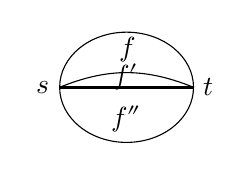
\begin{tikzpicture}[x=1cm,y=1cm,baseline=(current bounding box.center)] \draw (0,0) ellipse (0.85 and 0.70); \draw (-0.85,0) to[bend left=22] (0.85,0); \draw[line width=1.1pt] (-0.85,0)--(0.85,0); \node at (0,0.48) {$f$}; \node at (0,0.13) {$f'$}; \node at (0,-0.40) {$f''$}; \node[left] at (-0.85,0) {$s$}; \node[right] at (0.85,0) {$t$}; \end{tikzpicture}} $f\cap f''=\{s,t\}$} \var{\deleted{the}}{}{deletion}{ps_134-3_010-v0021}\var{\inserted{a}}{\hand{a}}{insertion}{ps_134-3_010-v0022} standard example\hand{.} \hand{\unsure{$\ell$}} \var{\over{o}{O}}{\hand{O}}{writing over}{ps_134-3_010-v0023}f lesser import is the misstatement \var{\inserted{(in section 2)}}{\hand{(in section 2)}}{insertion}{ps_134-3_010-v0024} \var{\deleted{on p.2'}}{}{deletion}{ps_134-3_010-v0025},
stating that the associativity relation for the operation \hand{$*_\ell$} should be
\var{\xout{wherex\allowbreak{}fx\allowbreak{}f"x\allowbreak{}isx\allowbreak{}ax\allowbreak{}two-pointx\allowbreak{}spacex\allowbreak{}$\underline{S}_o$x\allowbreak{}x\allowbreak{}x\allowbreak{}}}{}{typewriter deletion}{ps_134-3_010-v0026} replaced by a homotopy arrow
$(\hand{\lambda}*\hand{\mu})*\hand{\nu} \to \hand{\lambda}*(\hand{\mu}*\hand{\nu})$. This is OK for \hand{$\ell$}=1 (primary composition), but
already for \hand{$\ell$}=2 does not make sense as stated, because the sources and
the targets of the two compositions to be compared are not equal, but
only homotopic. Here the statement should be replaced by one making
sense, with a homotopy ``making commutative'' a certain square, and accor\hand{\unsure{-}}%
dingly for cubes etc for higher order co\var{\xout{mp}}{}{typewriter deletion}{ps_134-3_010-v0027}mpositions \hand{$\lambda *_\ell \mu$}, to give rea-%
sonable meaning to associativity. Anyhow, such painstaking explicita-%
tions of particular coherence properties (rather, coherence homotopies)
is kind of ruled out by the sweeping axiomatic description of the
kind of structure species we want for a ``stack'', at least\hand{,} I guess\hand{,} in

%% END SOURCE ps_134-3_010
\ifnum\EditionMode=1
\psapparatusstart
\psentry{ps_134-3_010-v0001}{1}{writing over}{\over{\unsure{18}}{18}}{\hand{18}}{The superposed handwritten reading replaces the underlying reading.}
\psentry{ps_134-3_010-v0002}{2}{insertion}{\inserted{(section 13)}}{\hand{(section 13)}}{The handwritten insertion is incorporated at its indicated position; insertion brackets leave the running text.}
\psentry{ps_134-3_010-v0003}{3}{deletion}{\deleted{\unsure{p.11'}}}{}{The author cancels this material by hand; it leaves the corrected running text.}
\psentry{ps_134-3_010-v0004}{4}{typewriter deletion}{\xout{thatxix}}{}{The typewriter strikes out this material; it leaves the corrected running text.}
\psentry{ps_134-3_010-v0005}{5}{typed insertion}{\inserted[typed]{(contractible)}}{(contractible)}{The typed insertion is incorporated at its indicated position; insertion brackets leave the running text.}
\psentry{ps_134-3_010-v0006}{6}{typewriter deletion}{\xout{x}}{}{The typewriter strikes out this material; it leaves the corrected running text.}
\psentry{ps_134-3_010-v0007}{7}{writing over}{\over{\unsure{at}}{ich}}{\hand{ich}}{The superposed handwritten reading replaces the underlying reading.}
\psentry{ps_134-3_010-v0008}{8}{typewriter deletion}{\xout{n}}{}{The typewriter strikes out this material; it leaves the corrected running text.}
\psentry{ps_134-3_010-v0009}{9}{typed insertion}{\inserted[typed]{strict}}{strict}{The typed insertion is incorporated at its indicated position; insertion brackets leave the running text.}
\psentry{ps_134-3_010-v0010}{10}{typewriter deletion}{\xout{x}}{}{The typewriter strikes out this material; it leaves the corrected running text.}
\psentry{ps_134-3_010-v0011}{11}{insertion}{\inserted{too}}{\hand{too}}{The handwritten insertion is incorporated at its indicated position; insertion brackets leave the running text.}
\psentry{ps_134-3_010-v0012}{12}{insertion}{\inserted{there}}{\hand{there}}{The handwritten insertion is incorporated at its indicated position; insertion brackets leave the running text.}
\psentry{ps_134-3_010-v0013}{13}{deletion}{\deleted{on p.11'}}{}{The author cancels this material by hand; it leaves the corrected running text.}
\psentry{ps_134-3_010-v0014}{14}{typewriter deletion}{\xout{xxxx}}{}{The typewriter strikes out this material; it leaves the corrected running text.}
\psentry{ps_134-3_010-v0015}{15}{typed insertion}{\inserted[typed]{total}}{total}{The typed insertion is incorporated at its indicated position; insertion brackets leave the running text.}
\psentry{ps_134-3_010-v0016}{16}{typewriter deletion}{\xout{xxxxxx}}{}{The typewriter strikes out this material; it leaves the corrected running text.}
\psentry{ps_134-3_010-v0017}{17}{insertion}{\inserted{(section 7)}}{\hand{(section 7)}}{The handwritten insertion is incorporated at its indicated position; insertion brackets leave the running text.}
\psentry{ps_134-3_010-v0018}{18}{deletion}{\deleted{p.7'}}{}{The author cancels this material by hand; it leaves the corrected running text.}
\psentry{ps_134-3_010-v0019}{19}{writing over}{\over{d}{y}}{\hand{y}}{The superposed handwritten reading replaces the underlying reading.}
\psentry{ps_134-3_010-v0020}{20}{typed insertion}{\inserted[typed]{maximal}}{maximal}{The typed insertion is incorporated at its indicated position; insertion brackets leave the running text.}
\psentry{ps_134-3_010-v0021}{21}{deletion}{\deleted{the}}{}{The author cancels this material by hand; it leaves the corrected running text.}
\psentry{ps_134-3_010-v0022}{22}{insertion}{\inserted{a}}{\hand{a}}{The handwritten insertion is incorporated at its indicated position; insertion brackets leave the running text.}
\psentry{ps_134-3_010-v0023}{23}{writing over}{\over{o}{O}}{\hand{O}}{The superposed handwritten reading replaces the underlying reading.}
\psentry{ps_134-3_010-v0024}{24}{insertion}{\inserted{(in section 2)}}{\hand{(in section 2)}}{The handwritten insertion is incorporated at its indicated position; insertion brackets leave the running text.}
\psentry{ps_134-3_010-v0025}{25}{deletion}{\deleted{on p.2'}}{}{The author cancels this material by hand; it leaves the corrected running text.}
\psentry{ps_134-3_010-v0026}{26}{typewriter deletion}{\xout{wherex\allowbreak{}fx\allowbreak{}f"x\allowbreak{}isx\allowbreak{}ax\allowbreak{}two-pointx\allowbreak{}spacex\allowbreak{}$\underline{S}_o$x\allowbreak{}x\allowbreak{}x\allowbreak{}}}{}{The typewriter strikes out this material; it leaves the corrected running text.}
\psentry{ps_134-3_010-v0027}{27}{typewriter deletion}{\xout{mp}}{}{The typewriter strikes out this material; it leaves the corrected running text.}
\psapparatusend
\fi
\pssource{ps_134-3_011}{134-3/11}{https://grothendieck.umontpellier.fr/web/viewer.html?file=../134-3.pdf\#page=12}
\psnumber{ps_134-3_011-v0001}{1}
\psnumber{ps_134-3_011-v0002}{2}
\psnumber{ps_134-3_011-v0003}{3}
\psnumber{ps_134-3_011-v0004}{4}
\psnumber{ps_134-3_011-v0005}{5}
\psnumber{ps_134-3_011-v0006}{6}
\psnumber{ps_134-3_011-v0007}{7}
\psnumber{ps_134-3_011-v0008}{8}
\psnumber{ps_134-3_011-v0009}{9}
\psnumber{ps_134-3_011-v0010}{10}
\psnumber{ps_134-3_011-v0011}{11}
\psnumber{ps_134-3_011-v0012}{12}
\psnumber{ps_134-3_011-v0013}{13}
\psnumber{ps_134-3_011-v0014}{14}
\psnumber{ps_134-3_011-v0015}{15}
\psnumber{ps_134-3_011-v0016}{16}
\psnumber{ps_134-3_011-v0017}{17}
\psnumber{ps_134-3_011-v0018}{18}
%% BEGIN SOURCE ps_134-3_011
% Pursuing Stacks (cotes 134-2 to 134-8): archive cote 134-3, site page 11 (PDF page 12), typescript page 11.
% typescript. Draft compared: ps2.tex:470-531.
% AI-transcribed by Claude Opus 5.5 (claude-opus-5-5, adaptive thinking, effort high), Message Batches API, batch ps1 (msgbatch_01Rv5hCaNTtUt4JHx1yqoHPL), 2026-11-12; image review recorded in records/CHECK_DECISIONS_134_3_4.tsv.
\scanpage{134-3/11}
\mspage{11}
a large part of the development of the theory of Gr-stacks.  A systematic
study of particular sets of homotopies is closely connected \var{\inserted{of course}}{\hand{of course}}{insertion}{ps_134-3_011-v0001} to an inves-%
\hand{(}tigation into irredundancy conditions which can be figured out for a
\var{\inserted{general}}{\hand{general}}{insertion}{ps_134-3_011-v0002} coherator $\underline{C}$ .  This is indeed an interesting topic,  but I decided not
to get involved in this,  unless I am really forced to!

The basic notion which has been peeling out in the reflection (L)
is of course the notion of a coherator.  Concerning terminology,  it oc-%
cured to me that the dual category $\underline{B}_\infty$ to $\underline{C}_\infty$ is more suggestive in some
cases,  for instance because of the topological interpretation attached
to its objects,  and (more technically)  because of formal analogy of
the role of this category,  for developping homotopical algebra,  with
\margin{(11)} the category of the standar\var{\over{\unsure{t}}{d}}{\hand{d}}{writing over}{ps_134-3_011-v0003} (ordered) simplices\hand{(\textsuperscript{11})}.Both mutually dual
objects $\underline{B}_\infty$ , $\underline{C}_\infty$ seem to me to merit a name,  I suggest to call them
respectively \uline{left} and \uline{right} \uline{coherat ors},  or simply \uline{coherators} of course
when for a while it is understood on which side of the mirror we \var{\over{are}{are}}{\hand{are}}{writing over}{ps_134-3_011-v0004}
playing the game.

O\var{\over{n}{n}}{\hand{n}}{writing over}{ps_134-3_011-v0005}e last comment still before taking off for a heuristic voyage
\var{\over{a}{o}}{\hand{o}}{writing over}{ps_134-3_011-v0006}f discovery of stacks\hand{!} I just had a glance at Benabou\hand{'}s expos\hand{\'e} in 1967
of \var{\over{W}{w}}{\hand{w}}{writing over}{ps_134-3_011-v0007}hat he calls ``bicategories''  (Springer Lecture N\var{\over{o}{o}}{\hand{o}}{writing over}{ps_134-3_011-v0008}tes n\textsuperscript{o} 47 ,  p. 1
- 77).  These are non else,  it appears\hand{,} \var{\deleted{\unsure{than}}}{}{deletion}{ps_134-3_011-v0009} than \var{\deleted{(}}{}{deletion}{ps_134-3_011-v0010}\uline{non associative}
2-categories,  namely 2-stacks  in the terminology I am proposing
(but not 2-Gr-stacks  -  namely at is a particular case of a general
notion of oo-stack which  has still to be developped).  The most interes-%
\hand{-}ting feature of this exposé,  it seems to me,  is the systematic refe-%
rence to topological intuition as \var{\inserted[typed]{a}}{a}{typed insertion}{ps_134-3_011-v0011} support for a comprehension of an
algebraic formalism,  notably \var{\inserted[typed]{of}}{of}{typed insertion}{ps_134-3_011-v0012} the structure of various diagrams. His
terminology,  referring to elements of $F_o,F_1,F_2$ respectively as 0-cells,
1-cells and 2-cells,  is quite suggestive of an idea of \var{\deleted{geometric}}{}{deletion}{ps_134-3_011-v0013} \var{\inserted[typed]{topological}}{topological}{typed insertion}{ps_134-3_011-v0014} reali-%
zation of a 2-stack  -  it is not clear from this exposé whether Benabou
has worked out this idea,  nor whether he has made a connection with
Quillen's ideas on axiomatics of homotopy theory,  which appeared the
same year in the same series\hand{(\textsuperscript{14})}. In any case,  in the last section of his
expos\hand{\'e},  he deals with his bicategories formally as with topological
spaces,  much in the same spirit as \hand{(}\var{\inserted{the one}}{\hand{the one}}{insertion}{ps_134-3_011-v0015} I was contemplating since \var{\xout{1975xxxxx}}{}{typewriter deletion}{ps_134-3_011-v0016}
around 1975,  and which is now motivating the present notes.  While
there is no mention of Benabou\hand{'}s ideas in my letters\var{\unsure{\deleted{t}}}{}{deletion}{ps_134-3_011-v0017} to Larry Breen,
it is quite possible that on the unconscious level,  the little I had
heard of his approach on one or two casual occasions,  had entered into
reaction with my own intuitions\hand{,} coming \var{\inserted[typed]{mainly}}{mainly}{typed insertion}{ps_134-3_011-v0018} from geometry and \unsure{hohomological|cohomological}
algebra,  and finally resulted in the program outlined in those letters.

%% END SOURCE ps_134-3_011
\ifnum\EditionMode=1
\psapparatusstart
\psentry{ps_134-3_011-v0001}{1}{insertion}{\inserted{of course}}{\hand{of course}}{The handwritten insertion is incorporated at its indicated position; insertion brackets leave the running text.}
\psentry{ps_134-3_011-v0002}{2}{insertion}{\inserted{general}}{\hand{general}}{The handwritten insertion is incorporated at its indicated position; insertion brackets leave the running text.}
\psentry{ps_134-3_011-v0003}{3}{writing over}{\over{\unsure{t}}{d}}{\hand{d}}{The superposed handwritten reading replaces the underlying reading.}
\psentry{ps_134-3_011-v0004}{4}{writing over}{\over{are}{are}}{\hand{are}}{The superposed handwritten reading replaces the underlying reading.}
\psentry{ps_134-3_011-v0005}{5}{writing over}{\over{n}{n}}{\hand{n}}{The superposed handwritten reading replaces the underlying reading.}
\psentry{ps_134-3_011-v0006}{6}{writing over}{\over{a}{o}}{\hand{o}}{The superposed handwritten reading replaces the underlying reading.}
\psentry{ps_134-3_011-v0007}{7}{writing over}{\over{W}{w}}{\hand{w}}{The superposed handwritten reading replaces the underlying reading.}
\psentry{ps_134-3_011-v0008}{8}{writing over}{\over{o}{o}}{\hand{o}}{The superposed handwritten reading replaces the underlying reading.}
\psentry{ps_134-3_011-v0009}{9}{deletion}{\deleted{\unsure{than}}}{}{The author cancels this material by hand; it leaves the corrected running text.}
\psentry{ps_134-3_011-v0010}{10}{deletion}{\deleted{(}}{}{The author cancels this material by hand; it leaves the corrected running text.}
\psentry{ps_134-3_011-v0011}{11}{typed insertion}{\inserted[typed]{a}}{a}{The typed insertion is incorporated at its indicated position; insertion brackets leave the running text.}
\psentry{ps_134-3_011-v0012}{12}{typed insertion}{\inserted[typed]{of}}{of}{The typed insertion is incorporated at its indicated position; insertion brackets leave the running text.}
\psentry{ps_134-3_011-v0013}{13}{deletion}{\deleted{geometric}}{}{The author cancels this material by hand; it leaves the corrected running text.}
\psentry{ps_134-3_011-v0014}{14}{typed insertion}{\inserted[typed]{topological}}{topological}{The typed insertion is incorporated at its indicated position; insertion brackets leave the running text.}
\psentry{ps_134-3_011-v0015}{15}{insertion}{\inserted{the one}}{\hand{the one}}{The handwritten insertion is incorporated at its indicated position; insertion brackets leave the running text.}
\psentry{ps_134-3_011-v0016}{16}{typewriter deletion}{\xout{1975xxxxx}}{}{The typewriter strikes out this material; it leaves the corrected running text.}
\psentry{ps_134-3_011-v0017}{17}{deletion}{\unsure{\deleted{t}}}{}{All material inside this wrapper is cancelled. Its original doubt and presentation remain in the diplomatic text and apparatus; no empty doubt mark or page label is inserted into the corrected running text.}
\psentry{ps_134-3_011-v0018}{18}{typed insertion}{\inserted[typed]{mainly}}{mainly}{The typed insertion is incorporated at its indicated position; insertion brackets leave the running text.}
\psapparatusend
\fi
\pssource{ps_134-3_012}{134-3/12}{https://grothendieck.umontpellier.fr/web/viewer.html?file=../134-3.pdf\#page=13}
\psnumber{ps_134-3_012-v0001}{1}
\psnumber{ps_134-3_012-v0002}{2}
\psnumber{ps_134-3_012-v0003}{3}
\psnumber{ps_134-3_012-v0004}{4}
\psnumber{ps_134-3_012-v0005}{5}
\psnumber{ps_134-3_012-v0006}{6}
\psnumber{ps_134-3_012-v0007}{7}
\psnumber{ps_134-3_012-v0008}{8}
\psnumber{ps_134-3_012-v0009}{9}
\psnumber{ps_134-3_012-v0010}{10}
\psnumber{ps_134-3_012-v0011}{11}
\psnumber{ps_134-3_012-v0012}{12}
\psnumber{ps_134-3_012-v0013}{13}
\psnumber{ps_134-3_012-v0014}{14}
\psnumber{ps_134-3_012-v0015}{15}
\psnumber{ps_134-3_012-v0016}{16}
\psnumber{ps_134-3_012-v0017}{17}
%% BEGIN SOURCE ps_134-3_012
% Pursuing Stacks (cotes 134-2 to 134-8): archive cote 134-3, site page 12 (PDF page 13), typescript page 12.
% typescript. Draft compared: ps2.tex:516-584.
% AI-transcribed by Claude Opus 5.5 (claude-opus-5-5, adaptive thinking, effort high), Message Batches API, batch ps1 (msgbatch_01Rv5hCaNTtUt4JHx1yqoHPL), 2026-11-12; image review recorded in records/CHECK_DECISIONS_134_3_4.tsv.
\scanpage{134-3/12}
\mspage{12}

\hand{19.} I would like now to write down a provisional itinerary of the \unsure{voyage}
ahead - namely to make a list of those main features of a theory of
\margin{$\times$} stacks which are in my mind these days. I will write them down in the
order in which they occur to me - which will be no obligation upon me
to follow this order, when coming back on those features separately to
elaborate somewhat on them\var{\over{,}{.}}{\hand{.}}{writing over}{ps_134-3_012-v0001} \var{\inserted{This I expect to do,}}{\hand{This I expect to do,}}{insertion}{ps_134-3_012-v0002} mainly as a way to check wether the main
notions and intuitions introduced are sound indeed, and otherwise, to
see how to correct them.

1\textsuperscript{o}) Definition of the categories $\underline{B}_o$ and its dual $\underline{C}_o$ , and formal defi-%
nition of left and right coherators. This definition \var{\over{\unsure{will}}{will}}{\hand{will}}{writing over}{ps_134-3_012-v0003} still be a
provisional one, and will presumably have to be adjusted somewhat to
\var{\over{allo}{allo}}{\hand{allo}}{writing over}{ps_134-3_012-v0004}w for the various structures we are looking for in the corresponding
category of Gr-stacks.

2\textsuperscript{o}) Relation between the category of Gr-stacks and the category of
topological spaces, via two adjoint functors, the ``topological realiza-%
tion functor'' $F_{\ast} \hand{\mapsto} \hand{|}F_{\ast}\hand{|}$ , and the ``singular stack functor''
$X \hand{\mapsto} \underline{F}_{\ast}(X)$ . The situation should be formally analogous to the corres-%
ponding situation for semi-simplicial sets versus topological spaces,
the role of the category $\underline{S}_{\ast}$ of standar\var{\over{t}{d}}{\hand{d}}{writing over}{ps_134-3_012-v0005} ordered simplices being taken
by the left coherator $\underline{B}$ we are working with. The main technical diffe-%
rence here is that the category of Gr-stacks is not just the category of
presheaves on $\underline{B}$, but the full subcategory defined by the requirement
that the presheaves considered should transform ``standar\var{\over{t}{d}}{\hand{d}}{writing over}{ps_134-3_012-v0006}'' amalgamated
sums into fibered products. As a matter of fact, the topological rea-%
lization functor $F_{\ast} \hand{\mapsto} \hand{|}F_{\ast}\hand{|}$ could be defined in standar\var{\over{t}{d}}{\hand{d}}{writing over}{ps_134-3_012-v0007} way on the
whole of $\hand{\widehat{\phantom{B}}}\underline{B}$ , in terms of any functor \var{\xout{B}}{}{typewriter deletion}{ps_134-3_012-v0008}
\hand{(*)} \[ \underline{B} \hand{\longrightarrow} \text{(Spaces)} \]
(by the requirement that the extension of this functor to $\hand{\widehat{\phantom{B}}}B$ commutes
with arbitrary direct limits). A second difference with the \var{\inserted{similar,}}{\hand{similar,}}{insertion}{ps_134-3_012-v0009} simplicial
\var{\deleted{similar}}{}{deletion}{ps_134-3_012-v0010} situation \var{\xout{is that}}{}{typewriter deletion}{ps_134-3_012-v0011} lies in the fact that the only really compel-%
ling choice for the functor (*) is it's restriction to $\underline{B}_o$ , in terms
of the cells $\underline{D}_n$ and the standart \hand{``}half-hemisphere \var{\xout{morphisms}}{}{typewriter deletion}{ps_134-3_012-v0012} maps\hand{''} between
these (L, \var{\deleted{\illegible{1}}}{}{deletion}{ps_134-3_012-v0013}\var{\inserted{section 6}}{\hand{section 6}}{insertion}{ps_134-3_012-v0014}). The extension of this functor to $\underline{B}$ is always possi\hand{\unsure{b}}%
le, due to the \var{\inserted[typed]{inductive}}{inductive}{typed insertion}{ps_134-3_012-v0015} construction of $\underline{B}$ and to the interpretation of elements
\margin{\diagram{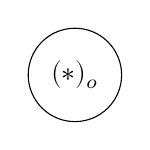
\begin{tikzpicture}[baseline=(n.base)]\node[draw,circle,inner sep=5pt] (n) {$({*})_o$};\end{tikzpicture}}} of $\underline{B}_o$ as \uline{contractible} spaces, via the functor (*)\hand{$_o$}; but it depends on
a bunch of arbitrary choices. To give precise meaning to the intuition
that these choices do\var{\over{nt}{'nt}}{\hand{'nt}}{writing over}{ps_134-3_012-v0016} really make a difference, and that the choic\unsure{e}
\var{\inserted[typed]{of}}{of}{typed insertion}{ps_134-3_012-v0017} coherator we are starting with does'nt make much of a difference either\hand{,}
will need some elaboration on the notion of \uline{equivalences between}

%% END SOURCE ps_134-3_012
\ifnum\EditionMode=1
\psapparatusstart
\psentry{ps_134-3_012-v0001}{1}{writing over}{\over{,}{.}}{\hand{.}}{The superposed handwritten reading replaces the underlying reading.}
\psentry{ps_134-3_012-v0002}{2}{insertion}{\inserted{This I expect to do,}}{\hand{This I expect to do,}}{The handwritten insertion is incorporated at its indicated position; insertion brackets leave the running text.}
\psentry{ps_134-3_012-v0003}{3}{writing over}{\over{\unsure{will}}{will}}{\hand{will}}{The superposed handwritten reading replaces the underlying reading.}
\psentry{ps_134-3_012-v0004}{4}{writing over}{\over{allo}{allo}}{\hand{allo}}{The superposed handwritten reading replaces the underlying reading.}
\psentry{ps_134-3_012-v0005}{5}{writing over}{\over{t}{d}}{\hand{d}}{The superposed handwritten reading replaces the underlying reading.}
\psentry{ps_134-3_012-v0006}{6}{writing over}{\over{t}{d}}{\hand{d}}{The superposed handwritten reading replaces the underlying reading.}
\psentry{ps_134-3_012-v0007}{7}{writing over}{\over{t}{d}}{\hand{d}}{The superposed handwritten reading replaces the underlying reading.}
\psentry{ps_134-3_012-v0008}{8}{typewriter deletion}{\xout{B}}{}{The typewriter strikes out this material; it leaves the corrected running text.}
\psentry{ps_134-3_012-v0009}{9}{insertion}{\inserted{similar,}}{\hand{similar,}}{The handwritten insertion is incorporated at its indicated position; insertion brackets leave the running text.}
\psentry{ps_134-3_012-v0010}{10}{deletion}{\deleted{similar}}{}{The author cancels this material by hand; it leaves the corrected running text.}
\psentry{ps_134-3_012-v0011}{11}{typewriter deletion}{\xout{is that}}{}{The typewriter strikes out this material; it leaves the corrected running text.}
\psentry{ps_134-3_012-v0012}{12}{typewriter deletion}{\xout{morphisms}}{}{The typewriter strikes out this material; it leaves the corrected running text.}
\psentry{ps_134-3_012-v0013}{13}{deletion}{\deleted{\illegible{1}}}{}{The author cancels this material by hand; it leaves the corrected running text.}
\psentry{ps_134-3_012-v0014}{14}{insertion}{\inserted{section 6}}{\hand{section 6}}{The handwritten insertion is incorporated at its indicated position; insertion brackets leave the running text.}
\psentry{ps_134-3_012-v0015}{15}{typed insertion}{\inserted[typed]{inductive}}{inductive}{The typed insertion is incorporated at its indicated position; insertion brackets leave the running text.}
\psentry{ps_134-3_012-v0016}{16}{writing over}{\over{nt}{'nt}}{\hand{'nt}}{The superposed handwritten reading replaces the underlying reading.}
\psentry{ps_134-3_012-v0017}{17}{typed insertion}{\inserted[typed]{of}}{of}{The typed insertion is incorporated at its indicated position; insertion brackets leave the running text.}
\psapparatusend
\fi
\pssource{ps_134-3_013}{134-3/13}{https://grothendieck.umontpellier.fr/web/viewer.html?file=../134-3.pdf\#page=14}
\psnumber{ps_134-3_013-v0001}{1}
\psnumber{ps_134-3_013-v0002}{2}
\psnumber{ps_134-3_013-v0003}{3}
\psnumber{ps_134-3_013-v0004}{4}
\psnumber{ps_134-3_013-v0005}{5}
\psnumber{ps_134-3_013-v0006}{6}
\psnumber{ps_134-3_013-v0007}{7}
\psnumber{ps_134-3_013-v0008}{8}
\psnumber{ps_134-3_013-v0009}{9}
\psnumber{ps_134-3_013-v0010}{10}
\psnumber{ps_134-3_013-v0011}{11}
\psnumber{ps_134-3_013-v0012}{12}
\psnumber{ps_134-3_013-v0013}{13}
\psnumber{ps_134-3_013-v0014}{14}
%% BEGIN SOURCE ps_134-3_013
% Pursuing Stacks (cotes 134-2 to 134-8): archive cote 134-3, site page 13 (PDF page 14), typescript page 13.
% typescript. Draft compared: ps2.tex:569-633.
% AI-transcribed by Claude Opus 5.5 (claude-opus-5-5, adaptive thinking, effort high), Message Batches API, batch ps1 (msgbatch_01Rv5hCaNTtUt4JHx1yqoHPL), 2026-11-12; image review recorded in records/CHECK_DECISIONS_134_3_4.tsv.
\scanpage{134-3/13}
\mspage{13}
Gr-\uline{stacks}, which will have to \var{\xout{tx}}{}{typewriter deletion}{ps_134-3_013-v0001} be developped at a later stage.

The idea just comes to my mind whether the exactness condition
implying standar\var{\over{t}{d}}{\hand{d}}{writing over}{ps_134-3_013-v0002} amalgamated sums, defining the subcategory of stacks
within $\overset{\hand{\wedge}}{\underline{B}}$ , cannot be interpreted in terms of some more or less obvious
topology on $\underline{B}$ turning $\underline{B}$ into a site, as the subcategory of correspon-%
ding \uline{sheaves}. This would mean that the category (Gr-stacks) is in fact
a topos, with the host of eategorical information and topological
intuition that goes with such a situation. In this connection, it is
timely to recall that the related categories (Cat) of ``all'' categories,
and (Groupoids) of ``all'' groupoids, are definitely \uline{not} topoi (if my
recollection is correct - it is\hand{'}nt immediately clear to me why they
are not). This seems to suggest that, granting that (Gr-stacks) is
indeed a topos, that this would be a rather special feature of the
structure species of infinite order we are working with (as \var{\deleted{a}}{}{deletion}{ps_134-3_013-v0003}\var{\inserted[typed]{one}}{one}{typed insertion}{ps_134-3_013-v0004} reward so
to say,among a heap of others, for conceptual sophistication !), in
contrast to the categories (Gr-n-stacks)\var{\inserted[typed]{with finite n}}{with finite n}{typed insertion}{ps_134-3_013-v0005}, which presumably are not topoi
(For a definition of Gr-n-stacks in terms of Gr-stacks namely
Gr-$\infty$-stacks, see below.\hand{)}

A related question is whether the category (Gr-stacks) is a model
category for the usual homotopy category, the pair of adjoint functors
bonsidered before satisfying \var{\inserted{moreover}}{\hand{moreover}}{insertion}{ps_134-3_013-v0006} the conditions of Quillen's comparison
theorem\hand{(\textsuperscript{13})}.The obvious idea that comes to mind here, in order to define
the model structure on (Gr-stacks), is to take as ``weak equivalences''
the maps which are transformed into weak equivalences by the topological
realization functor (which should be readily expressible in \var{\inserted[typed]{algebraic}}{algebraic}{typed insertion}{ps_134-3_013-v0007} terms \var{\xout{as}}{}{typewriter deletion}{ps_134-3_013-v0008} ..\hand{)},
\var{\over{\unsure{as}}{as}}{\hand{as}}{writing over}{ps_134-3_013-v0009} cofibrations the monomorphisms, and defining fibrations by the
Serre-Quillen lifting property with respect to cofibrations which are
weak equivalences (with the expectation that we even get a ``closed mod\hand{el}
category'' in the sense of Quillen). Here it does'nt look too unreasonab
\hand{-}le to expect the same constructions to work in each of the categories
(Gr-n-stacks), n \var{\over{$>$}{$\geqslant$}}{\hand{$\geqslant$}}{writing over}{ps_134-3_013-v0010}1, as well as in the categories (n-stacks) without
Gr , which are still to be defined though.

Coming back upon the question of a suitable topology on $\underline{B}$, the
idea that comes to mind immediately of course is to define\var{\deleted{s}}{}{deletion}{ps_134-3_013-v0011} covering
families of an object K of $\underline{B}$ i.e. of $\underline{B}_o$ , in terms of the components
which occur in the description of K as an \var{\inserted[typed]{iterated}}{iterated}{typed insertion}{ps_134-3_013-v0012} amalgamated sum of\var{\deleted{\unsure{s}}}{}{deletion}{ps_134-3_013-v0013} cells $D_n$.
A quick glance (too quick a glance ?) seems to show this is indeed a
topology, and that the sheaves for this topology are what we expect.
\var{\deleted{This would imply that the \deleted{inclusion} \inserted{composite} functor}}{}{deletion}{ps_134-3_013-v0014}

%% END SOURCE ps_134-3_013
\ifnum\EditionMode=1
\psapparatusstart
\psentry{ps_134-3_013-v0001}{1}{typewriter deletion}{\xout{tx}}{}{The typewriter strikes out this material; it leaves the corrected running text.}
\psentry{ps_134-3_013-v0002}{2}{writing over}{\over{t}{d}}{\hand{d}}{The superposed handwritten reading replaces the underlying reading.}
\psentry{ps_134-3_013-v0003}{3}{deletion}{\deleted{a}}{}{The author cancels this material by hand; it leaves the corrected running text.}
\psentry{ps_134-3_013-v0004}{4}{typed insertion}{\inserted[typed]{one}}{one}{The typed insertion is incorporated at its indicated position; insertion brackets leave the running text.}
\psentry{ps_134-3_013-v0005}{5}{typed insertion}{\inserted[typed]{with finite n}}{with finite n}{The typed insertion is incorporated at its indicated position; insertion brackets leave the running text.}
\psentry{ps_134-3_013-v0006}{6}{insertion}{\inserted{moreover}}{\hand{moreover}}{The handwritten insertion is incorporated at its indicated position; insertion brackets leave the running text.}
\psentry{ps_134-3_013-v0007}{7}{typed insertion}{\inserted[typed]{algebraic}}{algebraic}{The typed insertion is incorporated at its indicated position; insertion brackets leave the running text.}
\psentry{ps_134-3_013-v0008}{8}{typewriter deletion}{\xout{as}}{}{The typewriter strikes out this material; it leaves the corrected running text.}
\psentry{ps_134-3_013-v0009}{9}{writing over}{\over{\unsure{as}}{as}}{\hand{as}}{The superposed handwritten reading replaces the underlying reading.}
\psentry{ps_134-3_013-v0010}{10}{writing over}{\over{$>$}{$\geqslant$}}{\hand{$\geqslant$}}{The superposed handwritten reading replaces the underlying reading.}
\psentry{ps_134-3_013-v0011}{11}{deletion}{\deleted{s}}{}{The author cancels this material by hand; it leaves the corrected running text.}
\psentry{ps_134-3_013-v0012}{12}{typed insertion}{\inserted[typed]{iterated}}{iterated}{The typed insertion is incorporated at its indicated position; insertion brackets leave the running text.}
\psentry{ps_134-3_013-v0013}{13}{deletion}{\deleted{\unsure{s}}}{}{The author cancels this material by hand; it leaves the corrected running text.}
\psentry{ps_134-3_013-v0014}{14}{deletion}{\deleted{This would imply that the \deleted{inclusion} \inserted{composite} functor}}{}{The author cancels this material by hand; it leaves the corrected running text.}
\psapparatusend
\fi
\pssource{ps_134-3_014}{134-3/14}{https://grothendieck.umontpellier.fr/web/viewer.html?file=../134-3.pdf\#page=15}
\psnumber{ps_134-3_014-v0001}{1}
\psnumber{ps_134-3_014-v0002}{2}
\psnumber{ps_134-3_014-v0003}{3}
\psnumber{ps_134-3_014-v0004}{4}
\psnumber{ps_134-3_014-v0005}{5}
\psnumber{ps_134-3_014-v0006}{6}
\psnumber{ps_134-3_014-v0007}{7}
\psnumber{ps_134-3_014-v0008}{8}
\psnumber{ps_134-3_014-v0009}{9}
%% BEGIN SOURCE ps_134-3_014
% Pursuing Stacks (cotes 134-2 to 134-8): archive cote 134-3, site page 14 (PDF page 15), typescript page 14.
% typescript. Draft compared: ps2.tex:616-682.
% AI-transcribed by Claude Opus 5.5 (claude-opus-5-5, adaptive thinking, effort high), Message Batches API, batch ps1 (msgbatch_01Rv5hCaNTtUt4JHx1yqoHPL), 2026-11-12; image review recorded in records/CHECK_DECISIONS_134_3_4.tsv.
\scanpage{134-3/14}
\hand{5}.3. \mspage{\hand{14}}

\hand{20.} I had barely st opped writing last tuesday,  when it became clear \var{\xout{th}}{}{typewriter deletion}{ps_134-3_014-v0001}
that the ``quick glance'' had been too quick indeed. \var{\xout{It would}}{}{typewriter deletion}{ps_134-3_014-v0002} As a matter
of fact,  the ``topology'' I was contemplating on $\underline{B}$ in terms of covering
families does not satisfy the conditions for a ``site'' -  that something
was fishy first occured to me through the heuristic consequence,  that
the functors  ``n-th component''
\[ F_{*} \hand{\longmapsto} F_{n} \]
from \var{\xout{\illegible{1}}}{}{typewriter deletion}{ps_134-3_014-v0003} stacks to sets are fiber functors,  or equivalently, that
direct limits in the category of Gr-stacks can be computed componentwise
-  now this is definitely false,  for much the same reasons why it is
false \unsure{already|alfeady} in the category (Cat) of categories.  However,  it occured
to me that \var{\inserted{in}}{\hand{in}}{insertion}{ps_134-3_014-v0004} the latter category (Cat),  although not a topos (for instan-%
ce because, according to Giraud's paper on descent theory of 1965\hand{, (19)}
the implications for epimorphisms
\diagram{
% Hand-drawn arrows are marked blue; typed objects remain plain.
\begin{tikzcd}[row sep=tiny,column sep=large]
 \& \text{effective} \arrow[dr, Rightarrow, color=blue] \& \\
\text{effective universal} \arrow[ur, Rightarrow, color=blue] \arrow[dr, Rightarrow, color=blue] \& \& \text{just epi} \\
 \& \text{universal} \arrow[ur, Rightarrow, color=blue] \&
\end{tikzcd}
}
are strict),  there \uline{is} a very natural topology,  \var{\xout{namely}}{}{typewriter deletion}{ps_134-3_014-v0005} turning it into
a site,  namely the one where a family of morphisms namely functors
\[ A_{i} \hand{\longrightarrow} A \]
is covering if and only if the corresponding family in (Ss sets)
\[ \mathrm{Nerve}(A_{i}) \hand{\longrightarrow} \mathrm{Nerve}(A) \]
is covering,  i.e. iff every \var{\xout{family}}{}{typewriter deletion}{ps_134-3_014-v0006} sequence of composable arrows in A
\[ a_{0} \hand{\to} a_{1} \hand{\to} a_{2} \hand{\to} a_{3} \hand{\to} \quad \dots \hand{\to} a_{n} \]
can be lifted  to one among the $A_{i}$'s.  As a matter of fact,  this condi-%
\margin{\unsure{5.3. This is definitely false, see \S24 below}}
tion (where it suffices to take n=2,  visibly)  is equivalent (according
to Giraud) to the condition that the family be \hand{``}universally effectively
epimorphic\hand{''},  i.e. covering with respect to the``canonical topology''of
(Cat)\hand{(15)}.This suggests a third way for associating to a \var{\inserted{[small]}}{\hand{[small]}}{insertion}{ps_134-3_014-v0007} category A a
topology-like structure,  namely the topos of all sheaves over
$(\mathrm{Cat})_{/A}$  ,  the site of all categories over A, \var{\inserted[typed]{endowed}}{endowed}{typed insertion}{ps_134-3_014-v0008} with the topology induced
by the canonical topology of (Cat)  (which is indeed the canonical topo\hand{-}%
logy of  $(\mathrm{Cat})_{/A}$ \hand{)}.  It should be an easy exercice in terms of nerves to
check that the homotopy type (a priori,  a prohomotopy type)  associated
to this site is just \hand{``}the\hand{''}homotopy type of A,  defined either as the
homotopy type of Nerve(A),  or as the (pro)homotopy type of the topos
$\overset{\hand{\wedge}}{A}$ of all presheaves over A.  This of course parallels the similar fami-%
liar fact in the category (Ss sets) of all semisimplicial sets,  namely
that for such a ss set\var{\deleted{\unsure{s}}}{}{deletion}{ps_134-3_014-v0009} K,  the homotopy type of K can be viewed also
as the homotopy type of the induce\hand{d} topos  $(\mathrm{Ss\ sets})_{/K}$ of all ss sets
over K.  The difference in the two cases is that  in the second case

%% END SOURCE ps_134-3_014
\ifnum\EditionMode=1
\psapparatusstart
\psentry{ps_134-3_014-v0001}{1}{typewriter deletion}{\xout{th}}{}{The typewriter strikes out this material; it leaves the corrected running text.}
\psentry{ps_134-3_014-v0002}{2}{typewriter deletion}{\xout{It would}}{}{The typewriter strikes out this material; it leaves the corrected running text.}
\psentry{ps_134-3_014-v0003}{3}{typewriter deletion}{\xout{\illegible{1}}}{}{The typewriter strikes out this material; it leaves the corrected running text.}
\psentry{ps_134-3_014-v0004}{4}{insertion}{\inserted{in}}{\hand{in}}{The handwritten insertion is incorporated at its indicated position; insertion brackets leave the running text.}
\psentry{ps_134-3_014-v0005}{5}{typewriter deletion}{\xout{namely}}{}{The typewriter strikes out this material; it leaves the corrected running text.}
\psentry{ps_134-3_014-v0006}{6}{typewriter deletion}{\xout{family}}{}{The typewriter strikes out this material; it leaves the corrected running text.}
\psentry{ps_134-3_014-v0007}{7}{insertion}{\inserted{[small]}}{\hand{[small]}}{The handwritten insertion is incorporated at its indicated position; insertion brackets leave the running text.}
\psentry{ps_134-3_014-v0008}{8}{typed insertion}{\inserted[typed]{endowed}}{endowed}{The typed insertion is incorporated at its indicated position; insertion brackets leave the running text.}
\psentry{ps_134-3_014-v0009}{9}{deletion}{\deleted{\unsure{s}}}{}{The author cancels this material by hand; it leaves the corrected running text.}
\psapparatusend
\fi
\pssource{ps_134-3_015}{134-3/15}{https://grothendieck.umontpellier.fr/web/viewer.html?file=../134-3.pdf\#page=16}
\psnumber{ps_134-3_015-v0001}{1}
\psnumber{ps_134-3_015-v0002}{2}
\psnumber{ps_134-3_015-v0003}{3}
\psnumber{ps_134-3_015-v0004}{4}
\psnumber{ps_134-3_015-v0005}{5}
\psnumber{ps_134-3_015-v0006}{6}
\psnumber{ps_134-3_015-v0007}{7}
\psnumber{ps_134-3_015-v0008}{8}
\psnumber{ps_134-3_015-v0009}{9}
\psnumber{ps_134-3_015-v0010}{10}
\psnumber{ps_134-3_015-v0011}{11}
%% BEGIN SOURCE ps_134-3_015
% Pursuing Stacks (cotes 134-2 to 134-8): archive cote 134-3, site page 15 (PDF page 16), typescript page 15.
% typescript. Draft compared: ps2.tex:669-728.
% AI-transcribed by Claude Opus 5.5 (claude-opus-5-5, adaptive thinking, effort high), Message Batches API, batch ps1 (msgbatch_01Rv5hCaNTtUt4JHx1yqoHPL), 2026-11-12; image review recorded in records/CHECK_DECISIONS_134_3_4.tsv.
\scanpage{134-3/15}
\mspage{15}

the category  (Ss sets) (and hence \var{\over{\unsure{the}}{any}}{\hand{any}}{writing over}{ps_134-3_015-v0001} induced categor\var{\over{\unsure{ies}}{y}}{\hand{y}}{writing over}{ps_134-3_015-v0002}) \var{\over{\unsure{are}}{is}}{\hand{is}}{writing over}{ps_134-3_015-v0003} already
a topos,  namely equivalent to the category of sheaves on the same for
the canonical topology,  whereas in the category (Cat)  this is not so.

These reflections suggest that in most if not all categories of
models encountered for describing usual homotopy types,  there is a \margin{\unsure{5.3. this presumption is false actually}}
natural structure of a site on the model category M (\uline{presumably} the one
corresponding to the canonical topology(\var{\over{*}{15}}{\hand{15}}{writing over}{ps_134-3_015-v0004})), with the property that the
homotopy type of any object X in M is \var{\xout{also}}{}{typewriter deletion}{ps_134-3_015-v0005} canonically isomorphic to the
(pro)homotopy type of the induced site $M_{/X}$ ,  or what amount\hand{s} to the same,
of the corresponding topos
\[ (M_{/X})^{\hand{\sim}} \;=\; M^{\hand{\sim}}_{/X} \;. \]
I would expect definitely this to be the case for each of the categories
(Gr-stacks), (n-Gr-stacks) (although this is not really a model category
in the sense of Quillen,\hand{as} it gives rise only to n-truncated homotopy
types ...),  (stacks)  and (n-stacks),  corresponding to an arbitrary \margin{$\lceil$}
choice of a coherator,  defining the notion of a (Gr-stack),  or of a \margin{$[$}
stack  (for the latter and relations between the two,  see below). \margin{$\lfloor$}

\margin{$|$}\unsure{\var{\over{1}{2}}{\hand{2}}{writing over}{ps_134-3_015-v0006}}1.  I would like to digress a little more,  to emphasize still about
\margin{$\downarrow$}the vast variety of algebraic structures giving rise to model categories
for the usual homotopy category,  or at any rate suitable for expressing
more or less arbitrary homotopy types.  Apart from stacks,  where every
thing is still heuristics for the time being,  we have noticed so far
three examples of such structures,  namely  ss complexes,  cubical com-%
plexes,  and categories.  There are a  few familiar variants of the two
former,  such as the  ``simplicial complexes'' (in contrast to semi-simpli
cial ones) ,  namely \var{\inserted[typed]{presheaves on}}{presheaves on}{typed insertion}{ps_134-3_015-v0007} \var{\xout{functors from}}{}{typewriter deletion}{ps_134-3_015-v0008} the category of non-empty finite sets\hand{,}
which can be interpreted as ss complexes enriched with symmetry operati-%
ons on each component  -  and there is the corresponding variant in the
cubical case.  It would be rather surprising that these were not just
as good model categories,  as the more habitual ones (\var{\over{*}{16}}{\hand{16}}{writing over}{ps_134-3_015-v0009}) - all the more
as the singular complex (simplicial or cubical) is naturally endowed
with this extra structure,  which one generally chooses to forget. More
interesting variants are the  n-multicomplexes (simplicial or cubical,
with or without symmetries),  defined \hand{by} \var{\xout{presheaves}}{}{typewriter deletion}{ps_134-3_015-v0010} contravariant func-%
tors to sets  in n arguments rather than in just one,  where $n\hand{\geqslant}\hand{1}$. The-%
se complexes are familiar mainly,  it seems,  because of their connecti\hand{\unsure{on|ons}}
with product spaces and the Künneth-Eilenberg-Zilber type relations.
It is generally understood that to such a\var{\xout{n}}{}{typewriter deletion}{ps_134-3_015-v0011} multicomplex is associated

%% END SOURCE ps_134-3_015
\ifnum\EditionMode=1
\psapparatusstart
\psentry{ps_134-3_015-v0001}{1}{writing over}{\over{\unsure{the}}{any}}{\hand{any}}{The superposed handwritten reading replaces the underlying reading.}
\psentry{ps_134-3_015-v0002}{2}{writing over}{\over{\unsure{ies}}{y}}{\hand{y}}{The superposed handwritten reading replaces the underlying reading.}
\psentry{ps_134-3_015-v0003}{3}{writing over}{\over{\unsure{are}}{is}}{\hand{is}}{The superposed handwritten reading replaces the underlying reading.}
\psentry{ps_134-3_015-v0004}{4}{writing over}{\over{*}{15}}{\hand{15}}{The superposed handwritten reading replaces the underlying reading.}
\psentry{ps_134-3_015-v0005}{5}{typewriter deletion}{\xout{also}}{}{The typewriter strikes out this material; it leaves the corrected running text.}
\psentry{ps_134-3_015-v0006}{6}{writing over}{\over{1}{2}}{\hand{2}}{The superposed handwritten reading replaces the underlying reading.}
\psentry{ps_134-3_015-v0007}{7}{typed insertion}{\inserted[typed]{presheaves on}}{presheaves on}{The typed insertion is incorporated at its indicated position; insertion brackets leave the running text.}
\psentry{ps_134-3_015-v0008}{8}{typewriter deletion}{\xout{functors from}}{}{The typewriter strikes out this material; it leaves the corrected running text.}
\psentry{ps_134-3_015-v0009}{9}{writing over}{\over{*}{16}}{\hand{16}}{The superposed handwritten reading replaces the underlying reading.}
\psentry{ps_134-3_015-v0010}{10}{typewriter deletion}{\xout{presheaves}}{}{The typewriter strikes out this material; it leaves the corrected running text.}
\psentry{ps_134-3_015-v0011}{11}{typewriter deletion}{\xout{n}}{}{The typewriter strikes out this material; it leaves the corrected running text.}
\psapparatusend
\fi
\pssource{ps_134-3_016}{134-3/16}{https://grothendieck.umontpellier.fr/web/viewer.html?file=../134-3.pdf\#page=17}
\psnumber{ps_134-3_016-v0001}{1}
\psnumber{ps_134-3_016-v0002}{2}
\psnumber{ps_134-3_016-v0003}{3}
\psnumber{ps_134-3_016-v0004}{4}
\psnumber{ps_134-3_016-v0005}{5}
\psnumber{ps_134-3_016-v0006}{6}
\psnumber{ps_134-3_016-v0007}{7}
\psnumber{ps_134-3_016-v0008}{8}
\psnumber{ps_134-3_016-v0009}{9}
\psnumber{ps_134-3_016-v0010}{10}
\psnumber{ps_134-3_016-v0011}{11}
\psnumber{ps_134-3_016-v0012}{12}
\psnumber{ps_134-3_016-v0013}{13}
\psnumber{ps_134-3_016-v0014}{14}
\psnumber{ps_134-3_016-v0015}{15}
\psnumber{ps_134-3_016-v0016}{16}
\psnumber{ps_134-3_016-v0017}{17}
\psnumber{ps_134-3_016-v0018}{18}
\psnumber{ps_134-3_016-v0019}{19}
\psnumber{ps_134-3_016-v0020}{20}
\psnumber{ps_134-3_016-v0021}{21}
\psnumber{ps_134-3_016-v0022}{22}
\psnumber{ps_134-3_016-v0023}{23}
%% BEGIN SOURCE ps_134-3_016
% Pursuing Stacks (cotes 134-2 to 134-8): archive cote 134-3, site page 16 (PDF page 17), typescript page 16.
% typescript. Draft compared: ps2.tex:716-774.
% AI-transcribed by Claude Opus 5.5 (claude-opus-5-5, adaptive thinking, effort high), Message Batches API, batch ps1 (msgbatch_01Rv5hCaNTtUt4JHx1yqoHPL), 2026-11-12; image review recorded in records/CHECK_DECISIONS_134_3_4.tsv.
\scanpage{134-3/16}
\mspage{16}
the corresponding "diagonal" complex,  which is just a usual complex and
adequately describes the "homotopy type" of the multicomplex. So why
bother with relatively messy kind of models,  when just usual complexes
suffice !  Here however the point is not to get the handiest possible
model categories (whatever our cr\var{\over{e}{i}}{\hand{i}}{writing over}{ps_134-3_016-v0001}teria of "handyness"),  but rather to
get an idea of the variety of algebraic structures suitable for defining
homotopy types,  and perhaps to come to a clue of what is common to all
these.  Moreover,  I feel the relation between ordinary comple\var{\over{c}{x}}{\hand{x}}{writing over}{ps_134-3_016-v0002}es,
and n-multicomplexes,  is of much the same nature as the relation bet-%
ween just ordinary categories,  perfectly sufficient for describing homo
-topy types,  and  n-categories  or n-stacks.  This reminds of course of
Quillen's idea of defining n-categories in terms of n-semisimplicial
complexes,  in much the same way as categories can be defined (via the
Nerve functor)  in terms of usual ss complexes.  I hit again upon multi-%
simplices (without symmetry),  when trying to reduce to a \uline{minimum} the
\var{\over{category}{category}}{\hand{category}}{writing over}{ps_134-3_016-v0003} $\underline{B}_o$ of \var{\xout{\unsure{socalled}}}{}{typewriter deletion}{ps_134-3_016-v0004} what should be called "standar\var{\over{t}{d}}{\hand{d}}{writing over}{ps_134-3_016-v0005}"amalgamated
sums of the cells $D_n$ ,  where my tendency initially (L, \var{\deleted{\unsure{p.7}}}{}{deletion}{ps_134-3_016-v0006}\var{\inserted{section 8}}{\hand{section 8}}{insertion}{ps_134-3_016-v0007}) had rather
been to be as generous as possible,  in order to be as stringent as ima-%
ginable  for the completion condition (A)  of (L, \var{\deleted{\unsure{p.8}}}{}{deletion}{ps_134-3_016-v0008}\var{\inserted{section 9}}{\hand{section 9}}{insertion}{ps_134-3_016-v0009}).  Now it turns
out that the coherence relations which seem to have been written down so
far (and \var{\inserted[typed]{the like of}}{the like of}{typed insertion}{ps_134-3_016-v0010} which presumably will suffice to imply full completeness of
coherence relations,  in the sense of (A))  make use only of very restri-%
ted types of such amalgamated sums,  expressible precisely in terms of
multisimplices.  (This I ckecked \var{\inserted[typed]{for instance}}{for instance}{typed insertion}{ps_134-3_016-v0011} on the full list of data and axioms
for Bénabou's "bicategories" namely  2-stacks,  in \hand{his} 1967 Midwest Cate-%
gory Seminar \var{\inserted{exposé}}{\hand{exposé}}{insertion}{ps_134-3_016-v0012} (already referred to.)  I'll have to come back upon this
point with some care,  which gives also a pretty natural way for getting
Quillen's functor from  n-stacks to n-ss complexes.
\margin{\diagram{\begin{tikzpicture}[x=1cm,y=1cm]\draw[->] (0.35,0)--(0,0)--(0,1.1);\end{tikzpicture}}}

\margin{22.\diagram{\begin{tikzpicture}[x=1cm,y=1cm]\draw[->] (0.35,1.1)--(0,1.1)--(0,0);\end{tikzpicture}}} \var{\inserted{All}}{\hand{All}}{insertion}{ps_134-3_016-v0013} \var{\over{Th}{th}}{\hand{th}}{writing over}{ps_134-3_016-v0014}ese examples of possible models for homotopy types can be viewed
as generalizations of usual complexes,  or of usual categories\var{\over{.}{;}}{\hand{;}}{writing over}{ps_134-3_016-v0015}  I would
like to give a few others which go in the opposite direction\var{\deleted{s}}{}{deletion}{ps_134-3_016-v0016}  -  they
may be viewed as  \uline{particular cases} of categories.  One is the (pre)order
structure,  which may be viewed as a category structure when the
map    Fl \hand{$\longrightarrow$} Ob x Ob  defined by the source and target maps is injec-%
tive.  Such category is equivalent \var{\deleted{to}}{}{deletion}{ps_134-3_016-v0017} (and hence homotopic) to the
category associated with the corresponding \uline{ordered} set (when $x\hand{\geqslant} y$ and
$y\hand{\geqslant} x$ imply $x=y$)\var{\over{,}{.}}{\hand{.}}{writing over}{ps_134-3_016-v0018} \var{\deleted{which is}}{}{deletion}{ps_134-3_016-v0019} \var{\inserted{Ordered sets are}}{\hand{Ordered sets are}}{insertion}{ps_134-3_016-v0020} more familiar I guess as \var{\deleted{a}}{}{deletion}{ps_134-3_016-v0021} model object\hand{s} for
describing combinatorially a topological space,  in terms of a "cellular
subdivision"  by \var{\over{\illegible{1}}{compact}}{\hand{compact}}{writing over}{ps_134-3_016-v0022}\var{\inserted{(17)}}{\hand{(17)}}{insertion}{ps_134-3_016-v0023} subsets or "cells" ("strata" would be a more
\margin{$\times$}

%% END SOURCE ps_134-3_016
\ifnum\EditionMode=1
\psapparatusstart
\psentry{ps_134-3_016-v0001}{1}{writing over}{\over{e}{i}}{\hand{i}}{The superposed handwritten reading replaces the underlying reading.}
\psentry{ps_134-3_016-v0002}{2}{writing over}{\over{c}{x}}{\hand{x}}{The superposed handwritten reading replaces the underlying reading.}
\psentry{ps_134-3_016-v0003}{3}{writing over}{\over{category}{category}}{\hand{category}}{The superposed handwritten reading replaces the underlying reading.}
\psentry{ps_134-3_016-v0004}{4}{typewriter deletion}{\xout{\unsure{socalled}}}{}{The typewriter strikes out this material; it leaves the corrected running text.}
\psentry{ps_134-3_016-v0005}{5}{writing over}{\over{t}{d}}{\hand{d}}{The superposed handwritten reading replaces the underlying reading.}
\psentry{ps_134-3_016-v0006}{6}{deletion}{\deleted{\unsure{p.7}}}{}{The author cancels this material by hand; it leaves the corrected running text.}
\psentry{ps_134-3_016-v0007}{7}{insertion}{\inserted{section 8}}{\hand{section 8}}{The handwritten insertion is incorporated at its indicated position; insertion brackets leave the running text.}
\psentry{ps_134-3_016-v0008}{8}{deletion}{\deleted{\unsure{p.8}}}{}{The author cancels this material by hand; it leaves the corrected running text.}
\psentry{ps_134-3_016-v0009}{9}{insertion}{\inserted{section 9}}{\hand{section 9}}{The handwritten insertion is incorporated at its indicated position; insertion brackets leave the running text.}
\psentry{ps_134-3_016-v0010}{10}{typed insertion}{\inserted[typed]{the like of}}{the like of}{The typed insertion is incorporated at its indicated position; insertion brackets leave the running text.}
\psentry{ps_134-3_016-v0011}{11}{typed insertion}{\inserted[typed]{for instance}}{for instance}{The typed insertion is incorporated at its indicated position; insertion brackets leave the running text.}
\psentry{ps_134-3_016-v0012}{12}{insertion}{\inserted{exposé}}{\hand{exposé}}{The handwritten insertion is incorporated at its indicated position; insertion brackets leave the running text.}
\psentry{ps_134-3_016-v0013}{13}{insertion}{\inserted{All}}{\hand{All}}{The handwritten insertion is incorporated at its indicated position; insertion brackets leave the running text.}
\psentry{ps_134-3_016-v0014}{14}{writing over}{\over{Th}{th}}{\hand{th}}{The superposed handwritten reading replaces the underlying reading.}
\psentry{ps_134-3_016-v0015}{15}{writing over}{\over{.}{;}}{\hand{;}}{The superposed handwritten reading replaces the underlying reading.}
\psentry{ps_134-3_016-v0016}{16}{deletion}{\deleted{s}}{}{The author cancels this material by hand; it leaves the corrected running text.}
\psentry{ps_134-3_016-v0017}{17}{deletion}{\deleted{to}}{}{The author cancels this material by hand; it leaves the corrected running text.}
\psentry{ps_134-3_016-v0018}{18}{writing over}{\over{,}{.}}{\hand{.}}{The superposed handwritten reading replaces the underlying reading.}
\psentry{ps_134-3_016-v0019}{19}{deletion}{\deleted{which is}}{}{The author cancels this material by hand; it leaves the corrected running text.}
\psentry{ps_134-3_016-v0020}{20}{insertion}{\inserted{Ordered sets are}}{\hand{Ordered sets are}}{The handwritten insertion is incorporated at its indicated position; insertion brackets leave the running text.}
\psentry{ps_134-3_016-v0021}{21}{deletion}{\deleted{a}}{}{The author cancels this material by hand; it leaves the corrected running text.}
\psentry{ps_134-3_016-v0022}{22}{writing over}{\over{\illegible{1}}{compact}}{\hand{compact}}{The superposed handwritten reading replaces the underlying reading.}
\psentry{ps_134-3_016-v0023}{23}{insertion}{\inserted{(17)}}{\hand{(17)}}{The handwritten insertion is incorporated at its indicated position; insertion brackets leave the running text.}
\psapparatusend
\fi
\pssource{ps_134-3_017}{134-3/17}{https://grothendieck.umontpellier.fr/web/viewer.html?file=../134-3.pdf\#page=18}
\psnumber{ps_134-3_017-v0001}{1}
\psnumber{ps_134-3_017-v0002}{2}
\psnumber{ps_134-3_017-v0003}{3}
\psnumber{ps_134-3_017-v0004}{4}
\psnumber{ps_134-3_017-v0005}{5}
\psnumber{ps_134-3_017-v0006}{6}
\psnumber{ps_134-3_017-v0007}{7}
\psnumber{ps_134-3_017-v0008}{8}
\psnumber{ps_134-3_017-v0009}{9}
\psnumber{ps_134-3_017-v0010}{10}
\psnumber{ps_134-3_017-v0011}{11}
\psnumber{ps_134-3_017-v0012}{12}
\psnumber{ps_134-3_017-v0013}{13}
\psnumber{ps_134-3_017-v0014}{14}
\psnumber{ps_134-3_017-v0015}{15}
\psnumber{ps_134-3_017-v0016}{16}
\psnumber{ps_134-3_017-v0017}{17}
%% BEGIN SOURCE ps_134-3_017
% Pursuing Stacks (cotes 134-2 to 134-8): archive cote 134-3, site page 17 (PDF page 18), typescript page 17.
% typescript. Draft compared: ps2.tex:766-819.
% AI-transcribed by Claude Opus 5.5 (claude-opus-5-5, adaptive thinking, effort high), Message Batches API, batch ps1 (msgbatch_01Rv5hCaNTtUt4JHx1yqoHPL), 2026-11-12; image review recorded in records/CHECK_DECISIONS_134_3_4.tsv.
\scanpage{134-3/17}
\mspage{\hand{17}}

appropriate term\var{\xout{s}}{}{typewriter deletion}{ps_134-3_017-v0001}), which actually need not be topological cells in the
strict sense, but rather conical (and hence contractible) spaces,
each being homeomorphic to the cone \var{\deleted{defined}}{}{deletion}{ps_134-3_017-v0002} over the union of all strict-%
\margin{$\times$} ly smaller strata (this union is \uline{compact}). The ordered set associated
to such a (conically) stratified space X is just the set of \var{\inserted{[closed]}}{\hand{[closed]}}{insertion}{ps_134-3_017-v0003} strata,
with the inclusion relation, and it can be shown that there is a perfect
dictionary between the topological objects (at least in the case of
finite or locally finite stratifications), and the corresponding (finite
or locally finite) ordered sets, via a ``topological \uline{realization functor}''
\[ K \hand{\longrightarrow} \hand{|}K\hand{|} \]
from ordered sets to (conically stratified) topological spaces. As a
\margin{$\times$} matter of fact, when K is finite, \hand{|}K\hand{|} is endowed with a canonical
triangulation (the so-called barycentric subdivision), the combinato-%
rial model of which \var{\inserted{(or ``maquette'')}}{\hand{(or ``maquette'')}}{insertion}{ps_134-3_017-v0004} is as follows: the vertices are in one-to-one corres-%
pondance with the elements of K (they correspond to the vertices of the
corresponding cones), and the combinatorial simplices \var{\over{\unsure{are}}{are}}{\hand{are}}{writing over}{ps_134-3_017-v0005} the \var{\inserted{``flags'', or}}{\hand{``flags'', or}}{insertion}{ps_134-3_017-v0006} subsets
of K which are totally ordered for the induced order. This is still OK
when K is only locally finite (restricting of course to subsets of K
which are finite, when describing simplices), but in any case we can
define (via infinite direct limits\hand{\unsure{§}} in the category (Spaces) of all to-%
pological spaces) the geometric re\var{\over{a}{a}}{\hand{a}}{writing over}{ps_134-3_017-v0007}lization of K, \var{\deleted{and}}{}{deletion}{ps_134-3_017-v0008} together with
an interpretation of K as the ordered set of strata of \hand{|}K\hand{|} . As a mat-%
ter of fact, w\var{\over{\unsure{ea}}{e}}{\hand{e}}{writing over}{ps_134-3_017-v0009} get a canonical isomorphism (nearly tautological)
\[ \hand{|}K\hand{|} \hand{\xrightarrow{\sim}} \hand{|}\text{Nerve } K\hand{|} \hand{,} \]
where in the second member, we have writ\hand{t}en shortly K for the category
define\var{\over{\unsure{e}}{d}}{\hand{d}}{writing over}{ps_134-3_017-v0010} by K. I did not reflect whether it was reasonable to expect
that the categor\var{\over{y}{i}}{\hand{i}}{writing over}{ps_134-3_017-v0011}es (Preord) and (Ord) of preordered and ordered sets
are model categories, or even closed model categories, in Quillen's
precise sense - but it is clear though that using ordered sets we'll
get practi\var{\over{\unsure{u}}{c}}{\hand{c}}{writing over}{ps_134-3_017-v0012}ally any homotopy type, in any case any homotopy type which
can be described in terms of loca\var{\over{\unsure{l}}{ll}}{\hand{ll}}{writing over}{ps_134-3_017-v0013}y finite triangulations. However
it should be noted that the inclusion functors into (Cat) or (Ss sets)
\[ \margin{,}\ \text{\var{\over{\unsure{(Pr}}{(O}}{\hand{(O}}{writing over}{ps_134-3_017-v0014}rd)} \hand{\hookrightarrow} \text{(Pr\hand{e}ord)} \hand{\hookrightarrow} \text{(Cat)} \hand{\hookrightarrow} \text{(Ss sets)}\hand{,} \]
while giving the correct results on homotopy types, do not satisfy \var{\deleted{thex}}{}{deletion}{ps_134-3_017-v0015}
Quillen's general conditions on pairs of adjoint functors between model
categories - namely the adjoint functor say
\[ \text{(Cat)} \hand{\longrightarrow} \text{(Preord)}\hand{,} \]
associating to a category A the set Ob A with the obvious order relati-%
on, does \uline{not} commute to formation of homotopy types, as we see in the
trivial case when \var{\deleted{\unsure{thex}}}{}{deletion}{ps_134-3_017-v0016} Ob A \var{\inserted{[but not Fl(A)]}}{\hand{[but not Fl(A)]}}{insertion}{ps_134-3_017-v0017} is reduced to one point ...

%% END SOURCE ps_134-3_017
\ifnum\EditionMode=1
\psapparatusstart
\psentry{ps_134-3_017-v0001}{1}{typewriter deletion}{\xout{s}}{}{The typewriter strikes out this material; it leaves the corrected running text.}
\psentry{ps_134-3_017-v0002}{2}{deletion}{\deleted{defined}}{}{The author cancels this material by hand; it leaves the corrected running text.}
\psentry{ps_134-3_017-v0003}{3}{insertion}{\inserted{[closed]}}{\hand{[closed]}}{The handwritten insertion is incorporated at its indicated position; insertion brackets leave the running text.}
\psentry{ps_134-3_017-v0004}{4}{insertion}{\inserted{(or ``maquette'')}}{\hand{(or ``maquette'')}}{The handwritten insertion is incorporated at its indicated position; insertion brackets leave the running text.}
\psentry{ps_134-3_017-v0005}{5}{writing over}{\over{\unsure{are}}{are}}{\hand{are}}{The superposed handwritten reading replaces the underlying reading.}
\psentry{ps_134-3_017-v0006}{6}{insertion}{\inserted{``flags'', or}}{\hand{``flags'', or}}{The handwritten insertion is incorporated at its indicated position; insertion brackets leave the running text.}
\psentry{ps_134-3_017-v0007}{7}{writing over}{\over{a}{a}}{\hand{a}}{The superposed handwritten reading replaces the underlying reading.}
\psentry{ps_134-3_017-v0008}{8}{deletion}{\deleted{and}}{}{The author cancels this material by hand; it leaves the corrected running text.}
\psentry{ps_134-3_017-v0009}{9}{writing over}{\over{\unsure{ea}}{e}}{\hand{e}}{The superposed handwritten reading replaces the underlying reading.}
\psentry{ps_134-3_017-v0010}{10}{writing over}{\over{\unsure{e}}{d}}{\hand{d}}{The superposed handwritten reading replaces the underlying reading.}
\psentry{ps_134-3_017-v0011}{11}{writing over}{\over{y}{i}}{\hand{i}}{The superposed handwritten reading replaces the underlying reading.}
\psentry{ps_134-3_017-v0012}{12}{writing over}{\over{\unsure{u}}{c}}{\hand{c}}{The superposed handwritten reading replaces the underlying reading.}
\psentry{ps_134-3_017-v0013}{13}{writing over}{\over{\unsure{l}}{ll}}{\hand{ll}}{The superposed handwritten reading replaces the underlying reading.}
\psentry{ps_134-3_017-v0014}{14}{writing over}{\over{\unsure{(Pr}}{(O}}{\hand{(O}}{The superposed handwritten reading replaces the underlying reading.}
\psentry{ps_134-3_017-v0015}{15}{deletion}{\deleted{thex}}{}{The author cancels this material by hand; it leaves the corrected running text.}
\psentry{ps_134-3_017-v0016}{16}{deletion}{\deleted{\unsure{thex}}}{}{The author cancels this material by hand; it leaves the corrected running text.}
\psentry{ps_134-3_017-v0017}{17}{insertion}{\inserted{[but not Fl(A)]}}{\hand{[but not Fl(A)]}}{The handwritten insertion is incorporated at its indicated position; insertion brackets leave the running text.}
\psapparatusend
\fi
\pssource{ps_134-3_018}{134-3/18}{https://grothendieck.umontpellier.fr/web/viewer.html?file=../134-3.pdf\#page=19}
\psnumber{ps_134-3_018-v0001}{1}
\psnumber{ps_134-3_018-v0002}{2}
\psnumber{ps_134-3_018-v0003}{3}
\psnumber{ps_134-3_018-v0004}{4}
\psnumber{ps_134-3_018-v0005}{5}
\psnumber{ps_134-3_018-v0006}{6}
\psnumber{ps_134-3_018-v0007}{7}
\psnumber{ps_134-3_018-v0008}{8}
\psnumber{ps_134-3_018-v0009}{9}
\psnumber{ps_134-3_018-v0010}{10}
\psnumber{ps_134-3_018-v0011}{11}
\psnumber{ps_134-3_018-v0012}{12}
\psnumber{ps_134-3_018-v0013}{13}
\psnumber{ps_134-3_018-v0014}{14}
\psnumber{ps_134-3_018-v0015}{15}
\psnumber{ps_134-3_018-v0016}{16}
%% BEGIN SOURCE ps_134-3_018
% Pursuing Stacks (cotes 134-2 to 134-8): archive cote 134-3, site page 18 (PDF page 19), typescript page 18.
% typescript. Draft compared: ps2.tex:806-864.
% AI-transcribed by Claude Opus 5.5 (claude-opus-5-5, adaptive thinking, effort high), Message Batches API, batch ps1 (msgbatch_01Rv5hCaNTtUt4JHx1yqoHPL), 2026-11-12; image review recorded in records/CHECK_DECISIONS_134_3_4.tsv.
\scanpage{134-3/18}
\mspage{\hand{18}}

There is another amusing interpretation of the homotopy type associa-%
ted to any preordered set K,  via the topological space whose underlying
\margin{$\times$} set is K itself,  and where the closed sets are the subsets J of K
such that  $x \hand{\in} J$,  $y \hand{\subseteq} x$ implies $y \hand{\in} J$.  This is a highly non-separated
topology \var{\inserted{$\mathcal{T}$}}{\hand{$\mathcal{T}$}}{insertion}{ps_134-3_018-v0001} (except when the preorder relation is the discrete one),  where
an arbitrary union of closed subsets is again closed.  I doubt it's
singular homotopy type to make much sense,  however it's  homotopy type
as a topos does,  and (possibly under mild loc\unsure{\hand{-}}al finiteness restriction\unsure{s}\hand{)}
it should be the same as the homotopy type of K just envisioned.  Thus,
a sheaf on the topological space K  \var{\xout{defines}}{}{typewriter deletion}{ps_134-3_018-v0002} can be interpreted \var{\xout{as being}}{}{typewriter deletion}{ps_134-3_018-v0003}
\var{\over{v}{V}}{\hand{V}}{writing over}{ps_134-3_018-v0004}ia its fibers as being just a \uline{covariant} functor
\[ K \hand{\longrightarrow} (\text{Sets}) \]
(NB  the open sets of K are just the closed sets of $K^{o}$ , namely for the
opposite order relation,  and thus every $x \hand{\in} K$ has a smallest neighbour-%
hood,  namely the set \var{\xout{of all}}{}{typewriter deletion}{ps_134-3_018-v0005} $K_{\hand{\geq} x}$  of all $y \hand{\in} K$ such that $y \hand{\geq} x$),  or wh\hand{at}
amounts to the same,  a sheaf on the topos  $\overset{\hand{\wedge}}{K^{o}}$  defined by the opposite
order.  Hence the derived functors of the ``sections'' functor,  when
working with abelian sheaves \var{\inserted{on $(K,\mathcal{T})$}}{\hand{on $(K,\mathcal{T})$}}{insertion}{ps_134-3_018-v0006} \var{\xout{is just the}}{}{typewriter deletion}{ps_134-3_018-v0007} i.e.  the cohomology of the
topological space \var{\inserted{$(K,\mathcal{T})$}}{\hand{$(K,\mathcal{T})$}}{insertion}{ps_134-3_018-v0008} can be interpreted in terms of the topos associa-%
ted to $K^{o}$ .  This suggests that the definition I gave of the topology
of K was awkward and maybe it is indeed (although it is the more nat\var{\over{\unsure{y}}{u}}{\hand{u}}{writing over}{ps_134-3_018-v0009}ral
one in terms of incidence relations between open strata of $\hand{|}K\hand{|}$ ),\var{\inserted{and}}{\hand{and}}{insertion}{ps_134-3_018-v0010} that
we should have called ``open'' the sets I called ``closed'' and vide-versa,
or equivalently,  replace K by $K^{o}$ in the definition I gave of a topology
on the set K.  But as far as homotopy types are concerned, it does'nt
make a difference,  namely the homotopy types associated to K and $K^{o}$ are
canonically isomorphic.  This can be seen most simply on the topological
realizations,  via a homeomorphism (not only a homotopism)
\[ \hand{|}K\hand{|} \hand{\simeq} \hand{|}K^{o}\hand{|} , \]
coming from the fact that the maquettes (by which I mean the combinatori%
\margin{\diagram{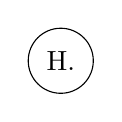
\begin{tikzpicture}[baseline=(n.base)]\node[draw,circle,inner sep=4pt] (n) {H.};\end{tikzpicture}}} al model  for a triangulation,  which \var{\inserted{H.}}{\hand{H.}}{insertion}{ps_134-3_018-v0011} Cartan time ago called ``schéma sim%
plicial'' ...) of the two spaces are canonically isomorphic,  because
the ``flags'' of K and $K^{o}$ are the same.  A similar argument due to Quillen
using the nerves shows that for any category K  (not necessarily ordered\unsure{\hand{)}}
K and $K^{o}$ are homotopic,  although \var{\inserted{$\widehat{K}$ and $\widehat{K^{o}}$ are}}{\hand{$\widehat{K}$ and $\widehat{K^{o}}$ are}}{insertion}{ps_134-3_018-v0012} definitely not equivalent i.e. \var{\inserted{not}}{\hand{not}}{insertion}{ps_134-3_018-v0013}
``homeomorphic'' .

To come back to the decreasing cascade of algebraic structures sui-%
table for describing homotopy types,  we could go down one more step
still,  to the category of  maquettes  (Maq) ,  namely sets \var{\inserted{S}}{\hand{S}}{insertion}{ps_134-3_018-v0014} together
with a family \var{\inserted{K}}{\hand{K}}{insertion}{ps_134-3_018-v0015} of finite subsets (the simplices\hand{\illegible{1}} of \var{\over{t}{t}}{\hand{t}}{writing over}{ps_134-3_018-v0016}he set of vertices

%% END SOURCE ps_134-3_018
\ifnum\EditionMode=1
\psapparatusstart
\psentry{ps_134-3_018-v0001}{1}{insertion}{\inserted{$\mathcal{T}$}}{\hand{$\mathcal{T}$}}{The handwritten insertion is incorporated at its indicated position; insertion brackets leave the running text.}
\psentry{ps_134-3_018-v0002}{2}{typewriter deletion}{\xout{defines}}{}{The typewriter strikes out this material; it leaves the corrected running text.}
\psentry{ps_134-3_018-v0003}{3}{typewriter deletion}{\xout{as being}}{}{The typewriter strikes out this material; it leaves the corrected running text.}
\psentry{ps_134-3_018-v0004}{4}{writing over}{\over{v}{V}}{\hand{V}}{The superposed handwritten reading replaces the underlying reading.}
\psentry{ps_134-3_018-v0005}{5}{typewriter deletion}{\xout{of all}}{}{The typewriter strikes out this material; it leaves the corrected running text.}
\psentry{ps_134-3_018-v0006}{6}{insertion}{\inserted{on $(K,\mathcal{T})$}}{\hand{on $(K,\mathcal{T})$}}{The handwritten insertion is incorporated at its indicated position; insertion brackets leave the running text.}
\psentry{ps_134-3_018-v0007}{7}{typewriter deletion}{\xout{is just the}}{}{The typewriter strikes out this material; it leaves the corrected running text.}
\psentry{ps_134-3_018-v0008}{8}{insertion}{\inserted{$(K,\mathcal{T})$}}{\hand{$(K,\mathcal{T})$}}{The handwritten insertion is incorporated at its indicated position; insertion brackets leave the running text.}
\psentry{ps_134-3_018-v0009}{9}{writing over}{\over{\unsure{y}}{u}}{\hand{u}}{The superposed handwritten reading replaces the underlying reading.}
\psentry{ps_134-3_018-v0010}{10}{insertion}{\inserted{and}}{\hand{and}}{The handwritten insertion is incorporated at its indicated position; insertion brackets leave the running text.}
\psentry{ps_134-3_018-v0011}{11}{insertion}{\inserted{H.}}{\hand{H.}}{The handwritten insertion is incorporated at its indicated position; insertion brackets leave the running text.}
\psentry{ps_134-3_018-v0012}{12}{insertion}{\inserted{$\widehat{K}$ and $\widehat{K^{o}}$ are}}{\hand{$\widehat{K}$ and $\widehat{K^{o}}$ are}}{The handwritten insertion is incorporated at its indicated position; insertion brackets leave the running text.}
\psentry{ps_134-3_018-v0013}{13}{insertion}{\inserted{not}}{\hand{not}}{The handwritten insertion is incorporated at its indicated position; insertion brackets leave the running text.}
\psentry{ps_134-3_018-v0014}{14}{insertion}{\inserted{S}}{\hand{S}}{The handwritten insertion is incorporated at its indicated position; insertion brackets leave the running text.}
\psentry{ps_134-3_018-v0015}{15}{insertion}{\inserted{K}}{\hand{K}}{The handwritten insertion is incorporated at its indicated position; insertion brackets leave the running text.}
\psentry{ps_134-3_018-v0016}{16}{writing over}{\over{t}{t}}{\hand{t}}{The superposed handwritten reading replaces the underlying reading.}
\psapparatusend
\fi
\pssource{ps_134-3_019}{134-3/19}{https://grothendieck.umontpellier.fr/web/viewer.html?file=../134-3.pdf\#page=20}
\psnumber{ps_134-3_019-v0001}{1}
\psnumber{ps_134-3_019-v0002}{2}
\psnumber{ps_134-3_019-v0003}{3}
\psnumber{ps_134-3_019-v0004}{4}
\psnumber{ps_134-3_019-v0005}{5}
\psnumber{ps_134-3_019-v0006}{6}
\psnumber{ps_134-3_019-v0007}{7}
\psnumber{ps_134-3_019-v0008}{8}
\psnumber{ps_134-3_019-v0009}{9}
%% BEGIN SOURCE ps_134-3_019
% Pursuing Stacks (cotes 134-2 to 134-8): archive cote 134-3, site page 19 (PDF page 20), typescript page 19.
% typescript. Draft compared: ps2.tex:851-922.
% AI-transcribed by Claude Opus 5.5 (claude-opus-5-5, adaptive thinking, effort high), Message Batches API, batch ps1 (msgbatch_01Rv5hCaNTtUt4JHx1yqoHPL), 2026-11-12; image review recorded in records/CHECK_DECISIONS_134_3_4.tsv.
\scanpage{134-3/19}
\mspage{\hand{19}}

S),  such that one-point subsets are simplices and a subset of a simplex
is a simplex.  This category,  via the functor   $(S,K)\hand{\mapsto} K$ ,  is equi-%
valent to the full subcategory of (Ord),  whose objects are those ordered
sets $K$,  such that for every $x\hand{\in}K$,  the set $K_{\hand{\leq}x}$  be isomorphic to the
\margin{\diagram{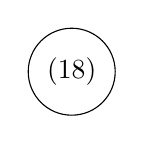
\begin{tikzpicture}[baseline=(n.base)]\node[draw,circle,inner sep=4pt] (n) {(18)};\end{tikzpicture}}}ordered set of \var{\xout{finite}}{}{typewriter deletion}{ps_134-3_019-v0001} non empty subsets of some finite set (or ``simplex'').
Here \var{\xout{again}}{}{typewriter deletion}{ps_134-3_019-v0002} the question \var{\xout{arises}}{}{typewriter deletion}{ps_134-3_019-v0003} whether  this category is a model category
in the technical sense \var{\inserted{[of Quillen]}}{\hand{[of Quillen]}}{insertion}{ps_134-3_019-v0004} does'nt really arise\hand{(18)}\hand{,} because this category
does'nt \var{\inserted{even}}{\hand{even}}{insertion}{ps_134-3_019-v0005} admit finite products -  rien à faire !
\margin{\unsure{\unsure{(17)} 5.3. indeed, the notion of a maquette is \uline{not} an algebraic structure species!}}

\var{\over{23}{23}}{\hand{23}}{writing over}{ps_134-3_019-v0006}.  It may be about time to get back to stacks,  still I can't help go-%
ing on pondering about algebraic structures as models for homotopy types.
If we have any algebraic structure species,  giving \var{\inserted{rise to}}{\hand{rise to}}{insertion}{ps_134-3_019-v0007} a category $M$ of
set-theoretic realizations,  the basic question here does'nt seem so
much whether $M$ is a model category for a suitable choice of the three
sets of arrows (fibrations,  cofibrations,  weak equivalences),  but
rather how to define a natural functor
\[ (*) \qquad M \hand{\longrightarrow} (\mathrm{Hot}) \hand{,} \]
where (Hot) is the category of usual homotopy types,  and see whether
via this functor (Hot) can be interpreted as a category of fractions
\hand{(}or ``localization''\hand{)}of $M$  -  namely,  of course,  by the operation of making
invertible those arrows in $M$ which are transformed into isomorphisms
in (Hot).  In any case,  if we have such a natural functor,  the natural
thing to do is to call those arrows ``weak equivalences''.  If we want $M$
\margin{\hand{(9)}}to be a category of models,  various examples suggest that the natural
thing again is to take as cofibrations the monomorphisms,\hand{(9)}\hand{,} and then
(expecting that the model categories we are going to meet will be closed
model categories) to define fibrations by the Serre-Quillen lifting pro-%
perty with respect to cofibrations (=monomorphisms) which are weak equi-%
valences.  This being done,  it becomes meaningful to ask if indeed $M$
is a category of models.

Now the reflections of the beginning of today's notes \var{\deleted{p.14-15}}{}{deletion}{ps_134-3_019-v0008} \var{\inserted{section 20}}{\hand{section 20}}{insertion}{ps_134-3_019-v0009}
suggest a rather natural way for describing a functor $(*)$,  which makes
\margin{\diagram{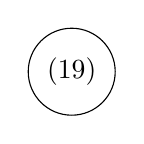
\begin{tikzpicture}[baseline=(n.base)]\node[draw,circle,inner sep=4pt] (n) {(19)};\end{tikzpicture}}}sense in fact,  in principle,  for any category $M$,  namely:  endow $M$ with
it's canonical topology (unless a still more natural one appears at hand\hand{(19)}
\margin{$($}\margin{\unsure{5.3. the canonical topology is \uline{not} always suitable, see \S 24 below}}-  I am not sure there is any better one in the present context),  and
assume that for every  $X\hand{\in}\mathrm{Ob}\,M$ ,  the pro-homotopy type of the induced
site  $M_{/X}$  is essentially constant,  i.e. can be identified with an
object in (Hot) itself.  We then get the functor $(*)$ in an obvious way.
It then becomes meaningful to ask whether this functor is a localization
functor.

When $M$ is defined in terms of an algebraic structure species,  it

%% END SOURCE ps_134-3_019
\ifnum\EditionMode=1
\psapparatusstart
\psentry{ps_134-3_019-v0001}{1}{typewriter deletion}{\xout{finite}}{}{The typewriter strikes out this material; it leaves the corrected running text.}
\psentry{ps_134-3_019-v0002}{2}{typewriter deletion}{\xout{again}}{}{The typewriter strikes out this material; it leaves the corrected running text.}
\psentry{ps_134-3_019-v0003}{3}{typewriter deletion}{\xout{arises}}{}{The typewriter strikes out this material; it leaves the corrected running text.}
\psentry{ps_134-3_019-v0004}{4}{insertion}{\inserted{[of Quillen]}}{\hand{[of Quillen]}}{The handwritten insertion is incorporated at its indicated position; insertion brackets leave the running text.}
\psentry{ps_134-3_019-v0005}{5}{insertion}{\inserted{even}}{\hand{even}}{The handwritten insertion is incorporated at its indicated position; insertion brackets leave the running text.}
\psentry{ps_134-3_019-v0006}{6}{writing over}{\over{23}{23}}{\hand{23}}{The superposed handwritten reading replaces the underlying reading.}
\psentry{ps_134-3_019-v0007}{7}{insertion}{\inserted{rise to}}{\hand{rise to}}{The handwritten insertion is incorporated at its indicated position; insertion brackets leave the running text.}
\psentry{ps_134-3_019-v0008}{8}{deletion}{\deleted{p.14-15}}{}{The author cancels this material by hand; it leaves the corrected running text.}
\psentry{ps_134-3_019-v0009}{9}{insertion}{\inserted{section 20}}{\hand{section 20}}{The handwritten insertion is incorporated at its indicated position; insertion brackets leave the running text.}
\psapparatusend
\fi
\pssource{ps_134-3_020}{134-3/20}{https://grothendieck.umontpellier.fr/web/viewer.html?file=../134-3.pdf\#page=21}
\psnumber{ps_134-3_020-v0001}{1}
\psnumber{ps_134-3_020-v0002}{2}
\psnumber{ps_134-3_020-v0003}{3}
\psnumber{ps_134-3_020-v0004}{4}
\psnumber{ps_134-3_020-v0005}{5}
\psnumber{ps_134-3_020-v0006}{6}
\psnumber{ps_134-3_020-v0007}{7}
\psnumber{ps_134-3_020-v0008}{8}
\psnumber{ps_134-3_020-v0009}{9}
\psnumber{ps_134-3_020-v0010}{10}
\psnumber{ps_134-3_020-v0011}{11}
\psnumber{ps_134-3_020-v0012}{12}
\psnumber{ps_134-3_020-v0013}{13}
%% BEGIN SOURCE ps_134-3_020
% Pursuing Stacks (cotes 134-2 to 134-8): archive cote 134-3, site page 20 (PDF page 21), typescript page 20.
% typescript. Draft compared: ps2.tex:909-968.
% AI-transcribed by Claude Opus 5.5 (claude-opus-5-5, adaptive thinking, effort high), Message Batches API, batch ps1 (msgbatch_01Rv5hCaNTtUt4JHx1yqoHPL), 2026-11-12; image review recorded in records/CHECK_DECISIONS_134_3_4.tsv.
\scanpage{134-3/20}
\mspage{\hand{20}}

admits both types of limits,  without finitesness requirement  -  and
we certainly would expect \var{\inserted[typed]{indeed}}{indeed}{typed insertion}{ps_134-3_020-v0001} at least existence of finite \uline{and} infinite di-%
rect sums in M,  if objects of M were to describe arbitrary homotopy
types.  However,  in view of the special exactness properties of (Hot),
which are by no means autodual,  we will expect moreover direct sums in
M to be ``universal and disjoint'',  in Giraud's sense.  This condition,
which caracterizes to a certain extent categories which at least mildly
resemble or parallel  categories such as (Sets), (Spaces) and similar
categories,whose objects more or less express ``shapes'' -  this condition
at once rules out the majority of the most common algebraic structures,
such as rings,  groups,\var{\xout{and the}}{}{typewriter deletion}{ps_134-3_020-v0002} modules over a ring or anything which
yields for M an abelian category,  etc.  If we describe an algebraic
structure species in terms of its universal realization in a category
stable under finite inverse limits,  then \var{\deleted{a}}{}{deletion}{ps_134-3_020-v0003}\var{\inserted[typed]{such}}{such}{typed insertion}{ps_134-3_020-v0004} structure species can be
viewed as being defined by such a category $\underline{C}$ , and its realizations in
\var{\inserted{any other such $C$ can be interpreted}}{\hand{any other such $C$ can be interpreted}}{insertion}{ps_134-3_020-v0005} \var{\deleted{C}}{}{deletion}{ps_134-3_020-v0006} as the left-exact functors $\underline{C}\hand{\to}C$ (the universal realization of the
structure within $\underline{C}$  corresponding to the identity functor $\underline{C}\hand{\Longrightarrow}\underline{C}$).  In
terms of the dual category $\underline{B}$ ,  associating to every element in
Ob $\underline{B}$  =  Ob $\underline{C}$  the covariant functor $\underline{C}\hand{\to}$(Sets) it represents,  we get
a fully-faithful embedding
\[ \underline{B}\hand{\hookrightarrow} M , \]
by which $\underline{B}$ can be interpreted as the \var{\inserted{category of the}}{\hand{category of the}}{insertion}{ps_134-3_020-v0007} (set-theoretic) realizations of
the given structure  which are of ``finite presentation'' in a suitable
sense (in terms of a given family of generators of $\underline{B}$ namely cogenerators
of $\underline{C}$,  considered as corresponding to the choice of ``base-sets'' for the
given structure species  -  \var{\xout{this}}{}{typewriter deletion}{ps_134-3_020-v0008}\var{\inserted[typed]{such}}{such}{typed insertion}{ps_134-3_020-v0009} choice however being considered as
a convenient way merely to describe the species in concrete terms ...).
\var{\over{I}{I}}{\hand{I}}{writing over}{ps_134-3_020-v0010}f I remember correctly,  M can \var{\over{b}{b}}{\hand{b}}{writing over}{ps_134-3_020-v0011}e deduced from $\underline{B}$,  up to equivalence,
as being merely the category of Ind-objects of $\underline{B}$ ,  i.e. the inclusion
functor above yields an equivalence of categories
\[ \mathrm{Ind}(\underline{B}) \hand{\xrightarrow{\approx}} M , \]
which implies, I guess\var{\xout{\illegible{1}}}{}{typewriter deletion}{ps_134-3_020-v0012},  that the exactness properties of M mainly
reflect those of $\underline{B}$ .  Thus I would expect the condition we want on direct
sums in M to correspond to the same condition for finite direct sums in
$\underline{B}$ ,  not more not less.  Thus the algebraic structure species satisfying
this condition should correspond exactly to small categories $\underline{B}$,  stable
under finite direct limits,  and such that finite sums in $\underline{B}$ are disjoint
and universal.   This condition is presumably necessary,  if we want the
functor (*) from M to Hot  to be defined and to be a localization func-%
tor  -   a condition which it would be nice to understand directly in \var{\xout{te}}{}{typewriter deletion}{ps_134-3_020-v0013}

%% END SOURCE ps_134-3_020
\ifnum\EditionMode=1
\psapparatusstart
\psentry{ps_134-3_020-v0001}{1}{typed insertion}{\inserted[typed]{indeed}}{indeed}{The typed insertion is incorporated at its indicated position; insertion brackets leave the running text.}
\psentry{ps_134-3_020-v0002}{2}{typewriter deletion}{\xout{and the}}{}{The typewriter strikes out this material; it leaves the corrected running text.}
\psentry{ps_134-3_020-v0003}{3}{deletion}{\deleted{a}}{}{The author cancels this material by hand; it leaves the corrected running text.}
\psentry{ps_134-3_020-v0004}{4}{typed insertion}{\inserted[typed]{such}}{such}{The typed insertion is incorporated at its indicated position; insertion brackets leave the running text.}
\psentry{ps_134-3_020-v0005}{5}{insertion}{\inserted{any other such $C$ can be interpreted}}{\hand{any other such $C$ can be interpreted}}{The handwritten insertion is incorporated at its indicated position; insertion brackets leave the running text.}
\psentry{ps_134-3_020-v0006}{6}{deletion}{\deleted{C}}{}{The author cancels this material by hand; it leaves the corrected running text.}
\psentry{ps_134-3_020-v0007}{7}{insertion}{\inserted{category of the}}{\hand{category of the}}{The handwritten insertion is incorporated at its indicated position; insertion brackets leave the running text.}
\psentry{ps_134-3_020-v0008}{8}{typewriter deletion}{\xout{this}}{}{The typewriter strikes out this material; it leaves the corrected running text.}
\psentry{ps_134-3_020-v0009}{9}{typed insertion}{\inserted[typed]{such}}{such}{The typed insertion is incorporated at its indicated position; insertion brackets leave the running text.}
\psentry{ps_134-3_020-v0010}{10}{writing over}{\over{I}{I}}{\hand{I}}{The superposed handwritten reading replaces the underlying reading.}
\psentry{ps_134-3_020-v0011}{11}{writing over}{\over{b}{b}}{\hand{b}}{The superposed handwritten reading replaces the underlying reading.}
\psentry{ps_134-3_020-v0012}{12}{typewriter deletion}{\xout{\illegible{1}}}{}{The typewriter strikes out this material; it leaves the corrected running text.}
\psentry{ps_134-3_020-v0013}{13}{typewriter deletion}{\xout{te}}{}{The typewriter strikes out this material; it leaves the corrected running text.}
\psapparatusend
\fi
\pssource{ps_134-3_021}{134-3/21}{https://grothendieck.umontpellier.fr/web/viewer.html?file=../134-3.pdf\#page=22}
\psnumber{ps_134-3_021-v0001}{1}
\psnumber{ps_134-3_021-v0002}{2}
\psnumber{ps_134-3_021-v0003}{3}
\psnumber{ps_134-3_021-v0004}{4}
\psnumber{ps_134-3_021-v0005}{5}
\psnumber{ps_134-3_021-v0006}{6}
\psnumber{ps_134-3_021-v0007}{7}
\psnumber{ps_134-3_021-v0008}{8}
\psnumber{ps_134-3_021-v0009}{9}
\psnumber{ps_134-3_021-v0010}{10}
\psnumber{ps_134-3_021-v0011}{11}
\psnumber{ps_134-3_021-v0012}{12}
\psnumber{ps_134-3_021-v0013}{13}
\psnumber{ps_134-3_021-v0014}{14}
\psnumber{ps_134-3_021-v0015}{15}
\psnumber{ps_134-3_021-v0016}{16}
\psnumber{ps_134-3_021-v0017}{17}
\psnumber{ps_134-3_021-v0018}{18}
\psnumber{ps_134-3_021-v0019}{19}
\psnumber{ps_134-3_021-v0020}{20}
\psnumber{ps_134-3_021-v0021}{21}
\psnumber{ps_134-3_021-v0022}{22}
\psnumber{ps_134-3_021-v0023}{23}
\psnumber{ps_134-3_021-v0024}{24}
\psnumber{ps_134-3_021-v0025}{25}
\psnumber{ps_134-3_021-v0026}{26}
%% BEGIN SOURCE ps_134-3_021
% Pursuing Stacks (cotes 134-2 to 134-8): archive cote 134-3, site page 21 (PDF page 22), typescript page 21.
% typescript. Draft compared: ps2.tex:955-1024.
% AI-transcribed by Claude Opus 5.5 (claude-opus-5-5, adaptive thinking, effort high), Message Batches API, batch ps1 (msgbatch_01Rv5hCaNTtUt4JHx1yqoHPL), 2026-11-12; image review recorded in records/CHECK_DECISIONS_134_3_4.tsv.
\scanpage{134-3/21}
\mspage{\hand{21}}

terms of $\underline{B}$ , and (presumably) in terms of the canonical topology\var{\inserted{(19)}}{\hand{(19)}}{insertion}{ps_134-3_021-v0001} of $\underline{B}$ ,
which should give rise to a\var{\xout{\unsure{xxxqui}}}{}{typewriter deletion}{ps_134-3_021-v0002} localization functor
\[ \underline{B} \hand{\longrightarrow} (\mathrm{Hot})_{\mathrm{f.t.}} \quad , \]
where the subscript f.t. means ``finite type'' - granting that the notion
of homotopy types of finite type (presumably the same as homotopy types
of finite triangulations,\var{\inserted{or}}{\hand{or}}{insertion}{ps_134-3_021-v0003} of \var{\inserted{``finite''}}{\hand{``finite''}}{insertion}{ps_134-3_021-v0004} C.W. spaces) is a well defined notion\var{\inserted{(20)}}{\hand{(20)}}{insertion}{ps_134-3_021-v0005}.
As usual, it is in $\underline{B}$ , not in $\underline{C}$ , that geometrical constructions
take place which make sense for topological intuition. More specifical-%
ly, it seems that in the cases met \var{\inserted{with}}{\hand{with}}{insertion}{ps_134-3_021-v0006} so far, there \uline{are} indeed privileged
base-sets for the structure species considered (such as the``components''
of a semi\var{\xout{s}}{}{typewriter deletion}{ps_134-3_021-v0007}simplicial of cubical complex, or of a stack, etc ), indexed
by the \var{\inserted[typed]{natural}}{natural}{typed insertion}{ps_134-3_021-v0008} integers or n-tupels of such integers, and which``correspond'' to
topological cells of various dimensions, \var{\deleted{the}}{}{deletion}{ps_134-3_021-v0009}\var{\inserted{Moreover,}}{\hand{Moreover,}}{insertion}{ps_134-3_021-v0010} some of the basic structu-%
ral \var{\inserted{monomorphic}}{\hand{monomorphic}}{insertion}{ps_134-3_021-v0011} maps between these \var{\inserted{objects of $\underline{B}$}}{\hand{objects of $\underline{B}$}}{insertion}{ps_134-3_021-v0012} defin\var{\over{ing}{e}}{\hand{e}}{writing over}{ps_134-3_021-v0013} cellular decompositions of the \var{\inserted[typed]{topological}}{topological}{typed insertion}{ps_134-3_021-v0014} spheres
bounding these topological cells. These objects and ``boundary\hand{*} maps''
between them \var{\deleted{\xout{form}}}{}{deletion}{ps_134-3_021-v0015}\var{\inserted[typed]{define}}{define}{typed insertion}{ps_134-3_021-v0016} a (non full, in general) subcategory of $\underline{B}$ , say $\underline{B}_{\mathrm{oo}}$ ,
which looks like the core of the category $\underline{B}$, from which the topological
significance of $\underline{B}$ is springing. It is in terms of $\underline{B}_{\mathrm{oo}}$ that the ``corres-%
pondance '' \hand{(}vaguely referred to above\hand{)} with topological cells \var{\inserted[typed]{and spheres}}{and spheres}{typed insertion}{ps_134-3_021-v0017} takes a
precise meaning. Namely, associating to any object of $\underline{B}_{\mathrm{oo}}$ the ordered
set of its subobjects (within $\underline{B}_{\mathrm{oo}}$ of course, not $\underline{B}$ ), the \var{\xout{conicalx}}{}{typewriter deletion}{ps_134-3_021-v0018}
(stratified) topological realization of this ordered set is a cell, and
the \var{\xout{union}}{}{typewriter deletion}{ps_134-3_021-v0019}\var{\inserted[typed]{family}}{family}{typed insertion}{ps_134-3_021-v0020} of \var{\deleted{\xout{the}}}{}{deletion}{ps_134-3_021-v0021} subcells of smaller dimension (namely different from
the given one) is a cellular subdivision of the \var{\inserted[typed]{sphere}}{sphere}{typed insertion}{ps_134-3_021-v0022} bounding th\var{\over{e}{is}}{\hand{is}}{writing over}{ps_134-3_021-v0023} cell\var{\inserted{(21)}}{\hand{(21)}}{insertion}{ps_134-3_021-v0024}.

\var{\over{\unsure{4}}{7}}{\hand{7}}{writing over}{ps_134-3_021-v0025}.3.
\var{\over{21}{24}}{\hand{24}}{writing over}{ps_134-3_021-v0026}. Yesterday there occured to me a big``étourderie'' again of the day
before, in connection with a reflection on a suitable ``natural'' site
structure on the category (Cat) - namely when asserting that for a
family of morphisms i.e. functors in (Cat)
\[ (*) \qquad A_i \hand{\longrightarrow} A \ , \]
in order for the corresponding family to be ``covering'' namely epimorphic
in the category (a topos, as a matter of fact) (Ss sets), namely for
the corresponding families of mappings of sets
\[ (**) \qquad \mathrm{Fl}_n(A_i) \hand{\longrightarrow} \mathrm{Fl}_n(A) \]
to be epimorphic, it was sufficient that this condition be satisfied
for n=2 (which, according to Giraud, just means that the family (*)
is covering for the canonical topology of (Cat)). This is obviously
false - morally, it would mean that an n-simplex is ``covered'' in a
reasonable sense by it's sub-2-simplices, which is pretty absurd. To

%% END SOURCE ps_134-3_021
\ifnum\EditionMode=1
\psapparatusstart
\psentry{ps_134-3_021-v0001}{1}{insertion}{\inserted{(19)}}{\hand{(19)}}{The handwritten insertion is incorporated at its indicated position; insertion brackets leave the running text.}
\psentry{ps_134-3_021-v0002}{2}{typewriter deletion}{\xout{\unsure{xxxqui}}}{}{The typewriter strikes out this material; it leaves the corrected running text.}
\psentry{ps_134-3_021-v0003}{3}{insertion}{\inserted{or}}{\hand{or}}{The handwritten insertion is incorporated at its indicated position; insertion brackets leave the running text.}
\psentry{ps_134-3_021-v0004}{4}{insertion}{\inserted{``finite''}}{\hand{``finite''}}{The handwritten insertion is incorporated at its indicated position; insertion brackets leave the running text.}
\psentry{ps_134-3_021-v0005}{5}{insertion}{\inserted{(20)}}{\hand{(20)}}{The handwritten insertion is incorporated at its indicated position; insertion brackets leave the running text.}
\psentry{ps_134-3_021-v0006}{6}{insertion}{\inserted{with}}{\hand{with}}{The handwritten insertion is incorporated at its indicated position; insertion brackets leave the running text.}
\psentry{ps_134-3_021-v0007}{7}{typewriter deletion}{\xout{s}}{}{The typewriter strikes out this material; it leaves the corrected running text.}
\psentry{ps_134-3_021-v0008}{8}{typed insertion}{\inserted[typed]{natural}}{natural}{The typed insertion is incorporated at its indicated position; insertion brackets leave the running text.}
\psentry{ps_134-3_021-v0009}{9}{deletion}{\deleted{the}}{}{The author cancels this material by hand; it leaves the corrected running text.}
\psentry{ps_134-3_021-v0010}{10}{insertion}{\inserted{Moreover,}}{\hand{Moreover,}}{The handwritten insertion is incorporated at its indicated position; insertion brackets leave the running text.}
\psentry{ps_134-3_021-v0011}{11}{insertion}{\inserted{monomorphic}}{\hand{monomorphic}}{The handwritten insertion is incorporated at its indicated position; insertion brackets leave the running text.}
\psentry{ps_134-3_021-v0012}{12}{insertion}{\inserted{objects of $\underline{B}$}}{\hand{objects of $\underline{B}$}}{The handwritten insertion is incorporated at its indicated position; insertion brackets leave the running text.}
\psentry{ps_134-3_021-v0013}{13}{writing over}{\over{ing}{e}}{\hand{e}}{The superposed handwritten reading replaces the underlying reading.}
\psentry{ps_134-3_021-v0014}{14}{typed insertion}{\inserted[typed]{topological}}{topological}{The typed insertion is incorporated at its indicated position; insertion brackets leave the running text.}
\psentry{ps_134-3_021-v0015}{15}{deletion}{\deleted{\xout{form}}}{}{The author cancels this material by hand; it leaves the corrected running text.}
\psentry{ps_134-3_021-v0016}{16}{typed insertion}{\inserted[typed]{define}}{define}{The typed insertion is incorporated at its indicated position; insertion brackets leave the running text.}
\psentry{ps_134-3_021-v0017}{17}{typed insertion}{\inserted[typed]{and spheres}}{and spheres}{The typed insertion is incorporated at its indicated position; insertion brackets leave the running text.}
\psentry{ps_134-3_021-v0018}{18}{typewriter deletion}{\xout{conicalx}}{}{The typewriter strikes out this material; it leaves the corrected running text.}
\psentry{ps_134-3_021-v0019}{19}{typewriter deletion}{\xout{union}}{}{The typewriter strikes out this material; it leaves the corrected running text.}
\psentry{ps_134-3_021-v0020}{20}{typed insertion}{\inserted[typed]{family}}{family}{The typed insertion is incorporated at its indicated position; insertion brackets leave the running text.}
\psentry{ps_134-3_021-v0021}{21}{deletion}{\deleted{\xout{the}}}{}{The author cancels this material by hand; it leaves the corrected running text.}
\psentry{ps_134-3_021-v0022}{22}{typed insertion}{\inserted[typed]{sphere}}{sphere}{The typed insertion is incorporated at its indicated position; insertion brackets leave the running text.}
\psentry{ps_134-3_021-v0023}{23}{writing over}{\over{e}{is}}{\hand{is}}{The superposed handwritten reading replaces the underlying reading.}
\psentry{ps_134-3_021-v0024}{24}{insertion}{\inserted{(21)}}{\hand{(21)}}{The handwritten insertion is incorporated at its indicated position; insertion brackets leave the running text.}
\psentry{ps_134-3_021-v0025}{25}{writing over}{\over{\unsure{4}}{7}}{\hand{7}}{The superposed handwritten reading replaces the underlying reading.}
\psentry{ps_134-3_021-v0026}{26}{writing over}{\over{21}{24}}{\hand{24}}{The superposed handwritten reading replaces the underlying reading.}
\psapparatusend
\fi
\pssource{ps_134-3_022}{134-3/22}{https://grothendieck.umontpellier.fr/web/viewer.html?file=../134-3.pdf\#page=23}
\psnumber{ps_134-3_022-v0001}{1}
\psnumber{ps_134-3_022-v0002}{2}
\psnumber{ps_134-3_022-v0003}{3}
\psnumber{ps_134-3_022-v0004}{4}
\psnumber{ps_134-3_022-v0005}{5}
\psnumber{ps_134-3_022-v0006}{6}
\psnumber{ps_134-3_022-v0007}{7}
\psnumber{ps_134-3_022-v0008}{8}
\psnumber{ps_134-3_022-v0009}{9}
\psnumber{ps_134-3_022-v0010}{10}
\psnumber{ps_134-3_022-v0011}{11}
%% BEGIN SOURCE ps_134-3_022
% Pursuing Stacks (cotes 134-2 to 134-8): archive cote 134-3, site page 22 (PDF page 23), typescript page 22.
% typescript. Draft compared: ps2.tex:1010-1069.
% AI-transcribed by Claude Opus 5.5 (claude-opus-5-5, adaptive thinking, effort high), Message Batches API, batch ps1 (msgbatch_01Rv5hCaNTtUt4JHx1yqoHPL), 2026-11-12; image review recorded in records/CHECK_DECISIONS_134_3_4.tsv.
\scanpage{134-3/22}
\mspage{\hand{22}}
give specific positive statements along these lines, let's \var{\inserted[typed]{for any $N\hand{\in}\underline{N}$,}}{for any $N\hand{\in}\underline{N}$,}{typed insertion}{ps_134-3_022-v0001} denote
by $T_N$ the topology on (Cat) for which a family (*) is covering i\var{\over{s}{ff}}{\hand{ff}}{writing over}{ps_134-3_022-v0002}
the families (**) are for $n\hand{\leqslant} N$ - which means also that the correspon-%
ding family of N-truncated nerves
\[ \mathrm{Nerve}(A_i)\hand{[}N\hand{]} \hand{\longrightarrow} \mathrm{Nerve}(A)\hand{[}N\hand{]} \]
is epimorphic. For N=1, this means that the family is \hand{``}universally
epimorphic\hand{''}, for N=2, that it is \var{\deleted{\unsure{it is|it as}}}{}{deletion}{ps_134-3_022-v0003}\hand{``}universally effectively epimor-%
phic\hand{''}i.e. covering for the canonical topology of (Cat) (Giraud, loc.
cit. page 28). It turns out that this decreasing sequence of topologies
on (Cat) is strictly decreasing - as a matter of fact, denoting by
$\hand{\Delta[}N\hand{]}$ the category of \var{\inserted[typed]{standart ordered}}{standart ordered}{typed insertion}{ps_134-3_022-v0004}\var{\xout{\illegible{1}}}{}{typewriter deletion}{ps_134-3_022-v0005}simplices of dimension $\hand{\leqslant} N$, and using the
inclusions
\[ \hand{\Delta[}N\hand{]\hookrightarrow}(\mathrm{Cat})\hand{\hookrightarrow\Delta}(N)\hand{^{\wedge}} \]
(for $N\hand{\geqslant}2$ say), an immediate application of the ``comparison lemma'' for
sites shows that we have an equivalence
\[ ((\mathrm{Cat}),T_N)\hand{^{\sim}\simeq\Delta[}N\hand{]^{\wedge}}, \]
and hence, for any object A in (Cat) namely any category A , we get
an equivalence
\[ ((\mathrm{Cat}),T_N)_{/A}\hand{)^{\sim}\simeq}(\hand{\Delta}(N)_{/A})\hand{^{\wedge}} \quad , \]
and hence the homotopy type of the first hand member is \var{\inserted{\uline{not}}}{\hand{\uline{not}}}{insertion}{ps_134-3_022-v0006} described by and
equivalent to the homotopy type of the whole Nerve(A) object, but
rather by its N-skeleton, which has the same homotopy and cohomology
invariants in \var{\inserted[typed]{dimension}}{dimension}{typed insertion}{ps_134-3_022-v0007} \var{\xout{degrees}}{}{typewriter deletion}{ps_134-3_022-v0008} $\hand{\leqslant} N$, but by no means for higher dimensions. This
shows that among the topologies $T_N$ , none is suitable for recovering
the homotopy type of objects of (Cat) in the way contemplated two days
ago (page 15); \var{\deleted{but}}{}{deletion}{ps_134-3_022-v0009} the one topology which \uline{is} suitable is the one which
may be denoted by $T_{\infty}$ , and which \var{\xout{wa}}{}{typewriter deletion}{ps_134-3_022-v0010}is the one indeed which I first con-%
templated (page 14), before the mistaken idea occured to me that it was
the same as the canonical topology.

A very similar mistake occured earlier, when I surmised that the \var{\inserted[typed]{left}}{left}{typed insertion}{ps_134-3_022-v0011}
adjoint functor N' to the inclusion or Nerve functor N from (Cat)
to (Ss sets) $=\hand{\Delta^{\wedge}}$ had the property that for any object K in (Ss sets),
K and N'(K) had same homotopy type. Looking up yesterday the descripti-%
on in Gabriel-Zisman of this functor, this recalled to my mind that
it factors (via the natural restriction functor) through the category
$(\hand{\Delta}[2])^{\wedge}$ , hence any morphism $K\hand{\longrightarrow}K'$ inducing an isomorphism on the
2-skeletons (which by no means implies that it is a homotopy equivalen-%
ce) induces an isomorphism $N'(K)\hand{\xrightarrow{\sim}}N'(K')$, and a fortiori a homotopy
equivalence. This shows that, even if it should be true that (Cat) is

%% END SOURCE ps_134-3_022
\ifnum\EditionMode=1
\psapparatusstart
\psentry{ps_134-3_022-v0001}{1}{typed insertion}{\inserted[typed]{for any $N\hand{\in}\underline{N}$,}}{for any $N\hand{\in}\underline{N}$,}{The typed insertion is incorporated at its indicated position; insertion brackets leave the running text.}
\psentry{ps_134-3_022-v0002}{2}{writing over}{\over{s}{ff}}{\hand{ff}}{The superposed handwritten reading replaces the underlying reading.}
\psentry{ps_134-3_022-v0003}{3}{deletion}{\deleted{\unsure{it is|it as}}}{}{The author cancels this material by hand; it leaves the corrected running text.}
\psentry{ps_134-3_022-v0004}{4}{typed insertion}{\inserted[typed]{standart ordered}}{standart ordered}{The typed insertion is incorporated at its indicated position; insertion brackets leave the running text.}
\psentry{ps_134-3_022-v0005}{5}{typewriter deletion}{\xout{\illegible{1}}}{}{The typewriter strikes out this material; it leaves the corrected running text.}
\psentry{ps_134-3_022-v0006}{6}{insertion}{\inserted{\uline{not}}}{\hand{\uline{not}}}{The handwritten insertion is incorporated at its indicated position; insertion brackets leave the running text.}
\psentry{ps_134-3_022-v0007}{7}{typed insertion}{\inserted[typed]{dimension}}{dimension}{The typed insertion is incorporated at its indicated position; insertion brackets leave the running text.}
\psentry{ps_134-3_022-v0008}{8}{typewriter deletion}{\xout{degrees}}{}{The typewriter strikes out this material; it leaves the corrected running text.}
\psentry{ps_134-3_022-v0009}{9}{deletion}{\deleted{but}}{}{The author cancels this material by hand; it leaves the corrected running text.}
\psentry{ps_134-3_022-v0010}{10}{typewriter deletion}{\xout{wa}}{}{The typewriter strikes out this material; it leaves the corrected running text.}
\psentry{ps_134-3_022-v0011}{11}{typed insertion}{\inserted[typed]{left}}{left}{The typed insertion is incorporated at its indicated position; insertion brackets leave the running text.}
\psapparatusend
\fi
\pssource{ps_134-3_023}{134-3/23}{https://grothendieck.umontpellier.fr/web/viewer.html?file=../134-3.pdf\#page=24}
\psnumber{ps_134-3_023-v0001}{1}
\psnumber{ps_134-3_023-v0002}{2}
\psnumber{ps_134-3_023-v0003}{3}
\psnumber{ps_134-3_023-v0004}{4}
\psnumber{ps_134-3_023-v0005}{5}
\psnumber{ps_134-3_023-v0006}{6}
\psnumber{ps_134-3_023-v0007}{7}
\psnumber{ps_134-3_023-v0008}{8}
\psnumber{ps_134-3_023-v0009}{9}
\psnumber{ps_134-3_023-v0010}{10}
\psnumber{ps_134-3_023-v0011}{11}
\psnumber{ps_134-3_023-v0012}{12}
\psnumber{ps_134-3_023-v0013}{13}
\psnumber{ps_134-3_023-v0014}{14}
\psnumber{ps_134-3_023-v0015}{15}
%% BEGIN SOURCE ps_134-3_023
% Pursuing Stacks (cotes 134-2 to 134-8): archive cote 134-3, site page 23 (PDF page 24), typescript page 23.
% typescript. Draft compared: ps2.tex:1055-1122.
% AI-transcribed by Claude Opus 5.5 (claude-opus-5-5, adaptive thinking, effort high), Message Batches API, batch ps1 (msgbatch_01Rv5hCaNTtUt4JHx1yqoHPL), 2026-11-12; image review recorded in records/CHECK_DECISIONS_134_3_4.tsv.
\scanpage{134-3/23}
\mspage{\hand{23}}
a model category in Quillen's sense,  the situation with the inclusion
functor
\[ N:(Cat)\hand{\longrightarrow} (Ss sets) \]
and the left adjoint functor N'  is by no means the one of Quillen\hand{'}s
comparison theorem,  where the two functors play\var{\xout{ed}}{}{typewriter deletion}{ps_134-3_023-v0001} mutually dual roles
and both induce equivalences on the corresponding localized homotopical
categories.  Here \uline{only} N,  \uline{not} N',  \uline{induces such equivalence}.  This is
analoguous to the situation,  already note\var{\over{\unsure{s}}{d}}{\hand{d}}{writing over}{ps_134-3_023-v0002} before,  of the inclusion
functors
\[ (Preord)\hand{\hookrightarrow} (Cat) \qquad or \qquad (Ord)\hand{\hookrightarrow} (Cat) \quad , \]
which \var{\inserted{[presumably]}}{\hand{[presumably]}}{insertion}{ps_134-3_023-v0003} by localization induce equivalences on the associated homotopy
categories,  but the left adjoint functors do not share this property.

The topology $T_\infty$  just considered on (Cat) as a ``suitable'' topology
for describing homotopy types of objects of (Cat),  was\hand{|}of course direct-%
ly inspired by the semi-simplicial approach to homotopy types,  via
simplicial complexes  namely via the two associated inclusion functors
\[ \hand{\Delta} \hand{\hookrightarrow} (Cat)\hand{\hookrightarrow} \hand{\Delta^{\wedge}} , \]
the second functor associating to every category A the ``complex'' of it's
``simplicial diagrams''  $a_o\hand{\longrightarrow} a_1\hand{\longrightarrow} \;\ldots\hand{\longrightarrow} a_n$ .  If we had been working
\var{\xout{rather}}{}{typewriter deletion}{ps_134-3_023-v0004} with  cubical complexes rather than ss ones for describing homoto
-py types,  this would give rise similarly to two functors
\[ \hand{\square} \hand{\hookrightarrow} (Cat)\hand{\hookrightarrow} \hand{\square^{\wedge}} , \]
where $\hand{\square}$ is the category of``standar\var{\over{t}{d}}{\hand{d}}{writing over}{ps_134-3_023-v0005} cubes'' and face and degeneracy
maps between them,  and where the second\hand{|}inclusion associates to every
category A the cubical complex of it's  ``cubical diagrams'',  namely \var{\inserted[typed]{commutative}}{commutative}{typed insertion}{ps_134-3_023-v0006}
diagrams in A modelled after the diagram types $\hand{\square}_n\hand{[}1\hand{]}$ ,  the 1-skeleton
of the standart n-cubes $\hand{\square}_n$ , with suitable orientations on it's edges
(indicative of the direction of corresponding arrows in A).  The natural
idea \var{\over{\xout{here}}{now}}{\hand{now}}{writing over}{ps_134-3_023-v0007} would be to endow (Cat) with the \var{\over{category}{topology}}{\hand{topology}}{writing over}{ps_134-3_023-v0008}, $T'_\infty$ say,  induced
by $\hand{\square^{\wedge}}$,  namely call a family (*)  covering iff for every $n\hand{\in} \underline{N}$,  the
corresponding family  of \var{\xout{set}}{}{typewriter deletion}{ps_134-3_023-v0009} maps of sets
\[ Cub_n(A_i)\hand{\longrightarrow} \hand{C}ub_n(A) \]
is epimorphic.   This \var{\xout{category}}{}{typewriter deletion}{ps_134-3_023-v0010} topology appears to be \var{\xout{finer}}{}{typewriter deletion}{ps_134-3_023-v0011}\var{\inserted[typed]{coarser}}{coarser}{typed insertion}{ps_134-3_023-v0012} than $T_\infty$ \var{\xout{,}}{}{typewriter deletion}{ps_134-3_023-v0013}
\var{\inserted[typed]{(i.e. there are less covering families),}}{(i.e. there are less covering families),}{typed insertion}{ps_134-3_023-v0014}
and the comparison lemma gives now the equivalence
\[ ((Cat),T'_\infty)\hand{^{\sim}} \hand{\simeq} \hand{\square^{\wedge}} , \]
which shows that definitely the topology is \uline{strictly} coarser than $T_\infty$ ,
as it gives rise to a non-equivalent topos,  $\hand{\square^{\wedge}}$ instead of $\hand{\Delta^{\wedge}}$.

T\var{\over{h}{h}}{\hand{h}}{writing over}{ps_134-3_023-v0015}ese reflections convince me  1)  there are indeed topologies
on (Cat),  suit\unsure{able for} describing the natural homotopy types of ob-%
jects of (Cat) namely of categories,  and  2)  that there is definitely

%% END SOURCE ps_134-3_023
\ifnum\EditionMode=1
\psapparatusstart
\psentry{ps_134-3_023-v0001}{1}{typewriter deletion}{\xout{ed}}{}{The typewriter strikes out this material; it leaves the corrected running text.}
\psentry{ps_134-3_023-v0002}{2}{writing over}{\over{\unsure{s}}{d}}{\hand{d}}{The superposed handwritten reading replaces the underlying reading.}
\psentry{ps_134-3_023-v0003}{3}{insertion}{\inserted{[presumably]}}{\hand{[presumably]}}{The handwritten insertion is incorporated at its indicated position; insertion brackets leave the running text.}
\psentry{ps_134-3_023-v0004}{4}{typewriter deletion}{\xout{rather}}{}{The typewriter strikes out this material; it leaves the corrected running text.}
\psentry{ps_134-3_023-v0005}{5}{writing over}{\over{t}{d}}{\hand{d}}{The superposed handwritten reading replaces the underlying reading.}
\psentry{ps_134-3_023-v0006}{6}{typed insertion}{\inserted[typed]{commutative}}{commutative}{The typed insertion is incorporated at its indicated position; insertion brackets leave the running text.}
\psentry{ps_134-3_023-v0007}{7}{writing over}{\over{\xout{here}}{now}}{\hand{now}}{The superposed handwritten reading replaces the underlying reading.}
\psentry{ps_134-3_023-v0008}{8}{writing over}{\over{category}{topology}}{\hand{topology}}{The superposed handwritten reading replaces the underlying reading.}
\psentry{ps_134-3_023-v0009}{9}{typewriter deletion}{\xout{set}}{}{The typewriter strikes out this material; it leaves the corrected running text.}
\psentry{ps_134-3_023-v0010}{10}{typewriter deletion}{\xout{category}}{}{The typewriter strikes out this material; it leaves the corrected running text.}
\psentry{ps_134-3_023-v0011}{11}{typewriter deletion}{\xout{finer}}{}{The typewriter strikes out this material; it leaves the corrected running text.}
\psentry{ps_134-3_023-v0012}{12}{typed insertion}{\inserted[typed]{coarser}}{coarser}{The typed insertion is incorporated at its indicated position; insertion brackets leave the running text.}
\psentry{ps_134-3_023-v0013}{13}{typewriter deletion}{\xout{,}}{}{The typewriter strikes out this material; it leaves the corrected running text.}
\psentry{ps_134-3_023-v0014}{14}{typed insertion}{\inserted[typed]{(i.e. there are less covering families),}}{(i.e. there are less covering families),}{The typed insertion is incorporated at its indicated position; insertion brackets leave the running text.}
\psentry{ps_134-3_023-v0015}{15}{writing over}{\over{h}{h}}{\hand{h}}{The superposed handwritten reading replaces the underlying reading.}
\psapparatusend
\fi
\pssource{ps_134-3_024}{134-3/24}{https://grothendieck.umontpellier.fr/web/viewer.html?file=../134-3.pdf\#page=25}
\psnumber{ps_134-3_024-v0001}{1}
\psnumber{ps_134-3_024-v0002}{2}
\psnumber{ps_134-3_024-v0003}{3}
\psnumber{ps_134-3_024-v0004}{4}
\psnumber{ps_134-3_024-v0005}{5}
\psnumber{ps_134-3_024-v0006}{6}
\psnumber{ps_134-3_024-v0007}{7}
\psnumber{ps_134-3_024-v0008}{8}
\psnumber{ps_134-3_024-v0009}{9}
\psnumber{ps_134-3_024-v0010}{10}
\psnumber{ps_134-3_024-v0011}{11}
\psnumber{ps_134-3_024-v0012}{12}
\psnumber{ps_134-3_024-v0013}{13}
\psnumber{ps_134-3_024-v0014}{14}
\psnumber{ps_134-3_024-v0015}{15}
\psnumber{ps_134-3_024-v0016}{16}
\psnumber{ps_134-3_024-v0017}{17}
\psnumber{ps_134-3_024-v0018}{18}
\psnumber{ps_134-3_024-v0019}{19}
\psnumber{ps_134-3_024-v0020}{20}
\psnumber{ps_134-3_024-v0021}{21}
\psnumber{ps_134-3_024-v0022}{22}
\psnumber{ps_134-3_024-v0023}{23}
\psnumber{ps_134-3_024-v0024}{24}
\psnumber{ps_134-3_024-v0025}{25}
%% BEGIN SOURCE ps_134-3_024
% Pursuing Stacks (cotes 134-2 to 134-8): archive cote 134-3, site page 24 (PDF page 25), typescript page 24.
% typescript. Draft compared: ps2.tex:1106-1172.
% AI-transcribed by Claude Opus 5.5 (claude-opus-5-5, adaptive thinking, effort high), Message Batches API, batch pilot (msgbatch_0189Nhf1xB615YWnztubtLfc), 2026-11-12; image review recorded in records/CHECK_DECISIONS_134_3_4.tsv.
\scanpage{134-3/24}
\mspage{24}
no privileged choice for such topology.  We just described two such,
but using \var{\xout{xx}}{}{typewriter deletion}{ps_134-3_024-v0001} multicomplexes (cubical or semisimplicial) rather than
\margin{\diagram{\begin{tikzpicture}[x=1cm,y=1cm]\draw[->] (0.35,0)--(0,0)--(0,0.8);\end{tikzpicture}}}simple complexes should give us infinitely \var{\inserted[typed]{many}}{many}{typed insertion}{ps_134-3_024-v0002} others  just as suitable,
and I suspect \var{\xout{that}}{}{typewriter deletion}{ps_134-3_024-v0003} now that there must be a big lot more of them still !

\margin{\diagram{\begin{tikzpicture}[x=1cm,y=1cm]\draw[->] (0.35,0.8)--(0,0.8)--(0,0);\end{tikzpicture}}}\var{\over{\illegible{1}}{25}}{\hand{25}}{writing over}{ps_134-3_024-v0004}.  A fortiori,  coming back to the intriguing question of \var{\xout{which}}{}{typewriter deletion}{ps_134-3_024-v0005} carac-%
terizing the algebraic structure species suitable for describing homoto-%
py types in the usual homotopy category (Hot),  \var{\xout{if M is the}}{}{typewriter deletion}{ps_134-3_024-v0006} and for
recovering (Hot) as a category of fractions of the category M of all
set-theoretic re\var{\xout{a}}{}{typewriter deletion}{ps_134-3_024-v0007}alizations of this species,  it becomes clear now that
we cannot hope reasonably for a ``natural'' topology on M,  distinguished
among all others,  giving rise to the wished-for functor
\[ (*) \qquad M \hand{\to} (\mathrm{Hot}) \]
in the way contemplated earlier (\var{\deleted{page 19 ff}}{}{deletion}{ps_134-3_024-v0008}\var{\inserted{section 23}}{\hand{section 23}}{insertion}{ps_134-3_024-v0009}).  Here it occu\var{\over{s}{r}}{\hand{r}}{writing over}{ps_134-3_024-v0010}s to me
that anyhow,  if concerned mainly with defining the functor (*),  we
should consider that two topologies T,T' on M such that $T \hand{\geqslant} T'$  and
hence giving rise to a morphism of topoi
\[ (**) \qquad M_T^{\hand{\sim}} \hand{\to} M_{T'}^{\hand{\sim}} \]
(the \var{\deleted{inverse}}{}{deletion}{ps_134-3_024-v0011}\var{\inserted{direct}}{\hand{direct}}{insertion}{ps_134-3_024-v0012} image functor associated to this morphism being the natural
inclusion functor\var{\xout{s}}{}{typewriter deletion}{ps_134-3_024-v0013}\hand{,} when considering T\var{\deleted{'}}{}{deletion}{ps_134-3_024-v0014}-sheaves as particular cases of
T\hand{'}-sheaves) are ``\uline{equivalent}''  -  maybe we should rather say ``\uline{Hot-equiva-}%
\uline{lent}'' -  if for any  object A in M,  the induced morphism
\var{\margin{\deleted{\illegible{1}}}}{}{marginal note revised}{ps_134-3_024-v0015}
\[ (M_T^{\hand{\sim}})_{/A} \hand{\to} (M_{T'}^{\hand{\sim}})_{/A} \]
\var{\margin{\deleted{\illegible{1}}}}{}{marginal note revised}{ps_134-3_024-v0016}
is a homotopy equivalence.  This can be viewed as an intrinsic property
of the morphism of topoi (**), of a type rather familiar I guess to
people used to the dial\var{\deleted{\unsure{l}}}{}{deletion}{ps_134-3_024-v0017}ectics of \hand{\'{}}etale cohomology,  where a very simi-%
lar notion was met and given the name of a ``globally acyclic morphism''.
The suitable name here would be ``globally\var{\xout{ acyclic}}{}{typewriter deletion}{ps_134-3_024-v0018} aspheric morphism''
which is a reinforcement of the former,  in the sense of being expressib%
le in terms of isomorphism\var{\xout{s}}{}{typewriter deletion}{ps_134-3_024-v0019} relations in cohomology with \var{\inserted{arbitrary}}{\hand{arbitrary}}{insertion}{ps_134-3_024-v0020} coefficient\var{\xout{s}}{}{typewriter deletion}{ps_134-3_024-v0021} \var{\inserted{sheaves}}{\hand{sheaves}}{insertion}{ps_134-3_024-v0022}
on the base,  \uline{including} \uline{non-commutative} coefficient sheaves\hand{(*\textsuperscript{22})}.The rela-%
tion just introduced between two topologies T,T' on a category M makes
sense for any M  (irresp\var{\xout{p}}{}{typewriter deletion}{ps_134-3_024-v0023}ective of the particular way M was introduced
here),  it is not yet an equivalence relation though  -  so why not
introduce the equivalence relation it generates,  and call this ``Hot-%
equivalence'' -  unless we find a still coarser,  and cleverer notion
of equivalence,  deserving this name.  The point which,  one feels now,
should be developped,  is that this notion of equivalence should be
the coarsest we can find out,  and which still implies that to any \var{\inserted[typed]{Hot-}}{Hot-}{typed insertion}{ps_134-3_024-v0024}equi-%
valence class of topologies on M there should be canonically associated
a functor  (*) ,  which should essentially he ``the'' common value of
all the similar functors,  associated to the topologies T within \var{\deleted{this}}{}{deletion}{ps_134-3_024-v0025}
\margin{\unsure{\diagram{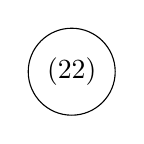
\begin{tikzpicture}[baseline=(n.base)]\node[draw,circle,inner sep=4pt] (n) {(22)};\end{tikzpicture}} * For a proper map of paracompact spaces, this condition just means that the fibers are ``aspheric'' namely ``contractible'' (in the Čech sense)}}

%% END SOURCE ps_134-3_024
\ifnum\EditionMode=1
\psapparatusstart
\psentry{ps_134-3_024-v0001}{1}{typewriter deletion}{\xout{xx}}{}{The typewriter strikes out this material; it leaves the corrected running text.}
\psentry{ps_134-3_024-v0002}{2}{typed insertion}{\inserted[typed]{many}}{many}{The typed insertion is incorporated at its indicated position; insertion brackets leave the running text.}
\psentry{ps_134-3_024-v0003}{3}{typewriter deletion}{\xout{that}}{}{The typewriter strikes out this material; it leaves the corrected running text.}
\psentry{ps_134-3_024-v0004}{4}{writing over}{\over{\illegible{1}}{25}}{\hand{25}}{The superposed handwritten reading replaces the underlying reading.}
\psentry{ps_134-3_024-v0005}{5}{typewriter deletion}{\xout{which}}{}{The typewriter strikes out this material; it leaves the corrected running text.}
\psentry{ps_134-3_024-v0006}{6}{typewriter deletion}{\xout{if M is the}}{}{The typewriter strikes out this material; it leaves the corrected running text.}
\psentry{ps_134-3_024-v0007}{7}{typewriter deletion}{\xout{a}}{}{The typewriter strikes out this material; it leaves the corrected running text.}
\psentry{ps_134-3_024-v0008}{8}{deletion}{\deleted{page 19 ff}}{}{The author cancels this material by hand; it leaves the corrected running text.}
\psentry{ps_134-3_024-v0009}{9}{insertion}{\inserted{section 23}}{\hand{section 23}}{The handwritten insertion is incorporated at its indicated position; insertion brackets leave the running text.}
\psentry{ps_134-3_024-v0010}{10}{writing over}{\over{s}{r}}{\hand{r}}{The superposed handwritten reading replaces the underlying reading.}
\psentry{ps_134-3_024-v0011}{11}{deletion}{\deleted{inverse}}{}{The author cancels this material by hand; it leaves the corrected running text.}
\psentry{ps_134-3_024-v0012}{12}{insertion}{\inserted{direct}}{\hand{direct}}{The handwritten insertion is incorporated at its indicated position; insertion brackets leave the running text.}
\psentry{ps_134-3_024-v0013}{13}{typewriter deletion}{\xout{s}}{}{The typewriter strikes out this material; it leaves the corrected running text.}
\psentry{ps_134-3_024-v0014}{14}{deletion}{\deleted{'}}{}{The author cancels this material by hand; it leaves the corrected running text.}
\psentry{ps_134-3_024-v0015}{15}{marginal note revised}{\margin{\deleted{\illegible{1}}}}{}{The author's internal cancellations and replacements in this marginal note are applied at its source-line call.}
\psentry{ps_134-3_024-v0016}{16}{marginal note revised}{\margin{\deleted{\illegible{1}}}}{}{The author's internal cancellations and replacements in this marginal note are applied at its source-line call.}
\psentry{ps_134-3_024-v0017}{17}{deletion}{\deleted{\unsure{l}}}{}{The author cancels this material by hand; it leaves the corrected running text.}
\psentry{ps_134-3_024-v0018}{18}{typewriter deletion}{\xout{ acyclic}}{}{The typewriter strikes out this material; it leaves the corrected running text.}
\psentry{ps_134-3_024-v0019}{19}{typewriter deletion}{\xout{s}}{}{The typewriter strikes out this material; it leaves the corrected running text.}
\psentry{ps_134-3_024-v0020}{20}{insertion}{\inserted{arbitrary}}{\hand{arbitrary}}{The handwritten insertion is incorporated at its indicated position; insertion brackets leave the running text.}
\psentry{ps_134-3_024-v0021}{21}{typewriter deletion}{\xout{s}}{}{The typewriter strikes out this material; it leaves the corrected running text.}
\psentry{ps_134-3_024-v0022}{22}{insertion}{\inserted{sheaves}}{\hand{sheaves}}{The handwritten insertion is incorporated at its indicated position; insertion brackets leave the running text.}
\psentry{ps_134-3_024-v0023}{23}{typewriter deletion}{\xout{p}}{}{The typewriter strikes out this material; it leaves the corrected running text.}
\psentry{ps_134-3_024-v0024}{24}{typed insertion}{\inserted[typed]{Hot-}}{Hot-}{The typed insertion is incorporated at its indicated position; insertion brackets leave the running text.}
\psentry{ps_134-3_024-v0025}{25}{deletion}{\deleted{this}}{}{The author cancels this material by hand; it leaves the corrected running text.}
\psapparatusend
\fi
\pssource{ps_134-3_025}{134-3/25}{https://grothendieck.umontpellier.fr/web/viewer.html?file=../134-3.pdf\#page=26}
\psnumber{ps_134-3_025-v0001}{1}
\psnumber{ps_134-3_025-v0002}{2}
\psnumber{ps_134-3_025-v0003}{3}
\psnumber{ps_134-3_025-v0004}{4}
\psnumber{ps_134-3_025-v0005}{5}
\psnumber{ps_134-3_025-v0006}{6}
\psnumber{ps_134-3_025-v0007}{7}
\psnumber{ps_134-3_025-v0008}{8}
\psnumber{ps_134-3_025-v0009}{9}
\psnumber{ps_134-3_025-v0010}{10}
\psnumber{ps_134-3_025-v0011}{11}
\psnumber{ps_134-3_025-v0012}{12}
\psnumber{ps_134-3_025-v0013}{13}
\psnumber{ps_134-3_025-v0014}{14}
\psnumber{ps_134-3_025-v0015}{15}
%% BEGIN SOURCE ps_134-3_025
% Pursuing Stacks (cotes 134-2 to 134-8): archive cote 134-3, site page 25 (PDF page 26), typescript page 25.
% typescript. Draft compared: ps2.tex:1160-1224.
% AI-transcribed by Claude Opus 5.5 (claude-opus-5-5, adaptive thinking, effort high), Message Batches API, batch ps1 (msgbatch_01Rv5hCaNTtUt4JHx1yqoHPL), 2026-11-12; image review recorded in records/CHECK_DECISIONS_134_3_4.tsv.
\scanpage{134-3/25}
\var{\xout{25}}{}{typewriter deletion}{ps_134-3_025-v0001}
\mspage{25}

this class.  Maybe even it could be shown that this equivalence class
can be recovered in terms of the corresponding functor (*),  in the same
way as (according to Giraud) a ``topology'' on M can be recovered from
the associated subtopos of $M^{\hand{\wedge}}$\hand{,}namely the associated category of sheaves
on M (in such a way that the set of \var{\xout{subcategor}}{}{typewriter deletion}{ps_134-3_025-v0002}``topologies''on M can be
identified with the set of \var{\xout{\unsure{subt}}}{}{typewriter deletion}{ps_134-3_025-v0003}``closed subtopoi'' of $M^{\hand{\wedge}}$).  The very best
one could possibly hope for along these lines would be a one-to-one
correspondance between isomorphism classes of functors (*)(satisfying
certain properties ?),  and the so-called ``Hot-equivalence classes'' of
topologies on M.

Whether or not this tentative hope is excessive, when it comes to
the (still somewhat vague) question of understanding ``which algebraic
structure species are suitable for expressing homotopy types'',  it
might not be excessive though to expect that in all \var{\inserted[typed]{such}}{such}{typed insertion}{ps_134-3_025-v0004} cases,  M should
be equipped with just \uline{one} ``natural'' Hot-equivalence class of topologies
\margin{\illegible{1}}on M\var{\deleted{\illegible{1}}}{}{deletion}{ps_134-3_025-v0005}\hand{,}which moreover (one hopes,  or wonders) should be expressible
directly in terms of the \var{\inserted[typed]{intrinsic}}{intrinsic}{typed insertion}{ps_134-3_025-v0006} structure of M,  or,  what amounts to the same,
in terms of the \var{\inserted[typed]{full}}{full}{typed insertion}{ps_134-3_025-v0007} subcategory $\underline{B}$ of objects of ``finite presentation'',  \var{\xout{\unsure{givi}}}{}{typewriter deletion}{ps_134-3_025-v0008}
giving rise to M via the equivalence
\[ M \hand{\simeq} \mathrm{Ind}(\underline{B}) . \]
As we just saw in the case  M = (Cat),  the so-called ``canonical topolo-%
gy'' on M need not be within the natural Hot-equivalence class  -  and I
am at a loss for the moment to give a plausible intrinsic caracterizati-%
on of the latter,  in terms of the category M = (Cat). \hand{(${}^{22'}$).}

\var{\over{\unsure{25}}{26}}{\hand{26}}{writing over}{ps_134-3_025-v0009}.  What comes to mind though is that the categories such as \hand{$\Delta$} , \hand{$\square$}
and their analogons (corresponding to multicomplexes rather than mono-%
complexes, for instance\var{\over{\unsure{,}}{)}}{\hand{)}}{writing over}{ps_134-3_025-v0010}  can be viewed as (generally not full) subcate-%
gories of M  (in fact,  even of the smaller category (Ord) of all orde\unsure{\hand{red}}
sets).  The topologies we found on M were in fact associated in an evi-%
dent way to the choice of such subcategories.  As was already felt by
the end of the reflection two days ago (p.21),  these subcategories
(denoted there by $\underline{B}_{oo}$  ) have rather special features  -  they are
associated to \var{\inserted[typed]{simultaneous}}{simultaneous}{typed insertion}{ps_134-3_025-v0011} cellular decompositions of spheres of all dimensions  -
and it is this feature,  presumably,  that makes the associated ``trivial''
algebraic structure \var{\inserted{species}}{\hand{species}}{insertion}{ps_134-3_025-v0012}, giving rise to the category of set-theoretic
realizations  $\underline{B}_{oo}{}^{\hand{\wedge}}$ ,  eligible for ``describing homotopy types''.  In the
typical example M = (Cat) though,  contrarily to what was suggested \hand{by}
\margin{\diagram{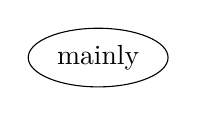
\begin{tikzpicture}[baseline=(n.base)]\node[draw,ellipse,inner sep=3pt] (n) {mainly};\end{tikzpicture}}}\var{\deleted{on page 21}}{}{deletion}{ps_134-3_025-v0013} \var{\inserted{the end of section 23}}{\hand{the end of section 23}}{insertion}{ps_134-3_025-v0014} (when thinking \var{\inserted{mainly}}{\hand{mainly}}{insertion}{ps_134-3_025-v0015} of the rather special although important cases
when M is expressible  as a category  $B^{\hand{\wedge}}$\hand{,} for some category B such as

%% END SOURCE ps_134-3_025
\ifnum\EditionMode=1
\psapparatusstart
\psentry{ps_134-3_025-v0001}{1}{typewriter deletion}{\xout{25}}{}{The typewriter strikes out this material; it leaves the corrected running text.}
\psentry{ps_134-3_025-v0002}{2}{typewriter deletion}{\xout{subcategor}}{}{The typewriter strikes out this material; it leaves the corrected running text.}
\psentry{ps_134-3_025-v0003}{3}{typewriter deletion}{\xout{\unsure{subt}}}{}{The typewriter strikes out this material; it leaves the corrected running text.}
\psentry{ps_134-3_025-v0004}{4}{typed insertion}{\inserted[typed]{such}}{such}{The typed insertion is incorporated at its indicated position; insertion brackets leave the running text.}
\psentry{ps_134-3_025-v0005}{5}{deletion}{\deleted{\illegible{1}}}{}{The author cancels this material by hand; it leaves the corrected running text.}
\psentry{ps_134-3_025-v0006}{6}{typed insertion}{\inserted[typed]{intrinsic}}{intrinsic}{The typed insertion is incorporated at its indicated position; insertion brackets leave the running text.}
\psentry{ps_134-3_025-v0007}{7}{typed insertion}{\inserted[typed]{full}}{full}{The typed insertion is incorporated at its indicated position; insertion brackets leave the running text.}
\psentry{ps_134-3_025-v0008}{8}{typewriter deletion}{\xout{\unsure{givi}}}{}{The typewriter strikes out this material; it leaves the corrected running text.}
\psentry{ps_134-3_025-v0009}{9}{writing over}{\over{\unsure{25}}{26}}{\hand{26}}{The superposed handwritten reading replaces the underlying reading.}
\psentry{ps_134-3_025-v0010}{10}{writing over}{\over{\unsure{,}}{)}}{\hand{)}}{The superposed handwritten reading replaces the underlying reading.}
\psentry{ps_134-3_025-v0011}{11}{typed insertion}{\inserted[typed]{simultaneous}}{simultaneous}{The typed insertion is incorporated at its indicated position; insertion brackets leave the running text.}
\psentry{ps_134-3_025-v0012}{12}{insertion}{\inserted{species}}{\hand{species}}{The handwritten insertion is incorporated at its indicated position; insertion brackets leave the running text.}
\psentry{ps_134-3_025-v0013}{13}{deletion}{\deleted{on page 21}}{}{The author cancels this material by hand; it leaves the corrected running text.}
\psentry{ps_134-3_025-v0014}{14}{insertion}{\inserted{the end of section 23}}{\hand{the end of section 23}}{The handwritten insertion is incorporated at its indicated position; insertion brackets leave the running text.}
\psentry{ps_134-3_025-v0015}{15}{insertion}{\inserted{mainly}}{\hand{mainly}}{The handwritten insertion is incorporated at its indicated position; insertion brackets leave the running text.}
\psapparatusend
\fi
\pssource{ps_134-3_026}{134-3/26}{https://grothendieck.umontpellier.fr/web/viewer.html?file=../134-3.pdf\#page=27}
\psnumber{ps_134-3_026-v0001}{1}
\psnumber{ps_134-3_026-v0002}{2}
\psnumber{ps_134-3_026-v0003}{3}
\psnumber{ps_134-3_026-v0004}{4}
\psnumber{ps_134-3_026-v0005}{5}
%% BEGIN SOURCE ps_134-3_026
% Pursuing Stacks (cotes 134-2 to 134-8): archive cote 134-3, site page 26 (PDF page 27), typescript page 26.
% typescript. Draft compared: ps2.tex:1210-1267.
% AI-transcribed by Claude Opus 5.5 (claude-opus-5-5, adaptive thinking, effort high), Message Batches API, batch ps1 (msgbatch_01Rv5hCaNTtUt4JHx1yqoHPL), 2026-11-12; image review recorded in records/CHECK_DECISIONS_134_3_4.tsv.
\scanpage{134-3/26}
\mspage{26}

\hand{$\Delta$} ,\hand{$\square$} etc), there is no really privileged choice of such subcategory
$\underline{B}_{oo}$ - we found indeed a big bunch of such, the ones just as good as
the others. The point of course is that the corresponding topologies
on M, namely induced from the canonical topology on $\underline{B}_{oo}\hand{\hat{}}$ by the canoni-%
cal functor
\[ M \hand{\longrightarrow} \underline{B}_{oo}\hand{\hat{}} \quad , \]
are Hot-equivalent for some reason or other, which should be understood.
The plausible fact that emerges here, is that the ``natural'' Hot-equi-%
valence class of topologies on M is associated, in the way just descri-%
bed, to a \uline{class} (presumably an equivalence class in a suitable set for
suitable equivalence relation ...) \uline{of subcategories} $\underline{B}_{oo}$ \uline{in} M. The ques-%
tion of giving an intrinsic description of the former, is apparently
reduced to the (possibly more concrete) one, of giving an intrinsic
\unsure{descripttion|description} of a bunch of subcategories \var{\inserted[typed]{$B =$}}{$B =$}{typed insertion}{ps_134-3_026-v0001}$\underline{B}_{oo}$ of M. This description,
one feels, should both a) insist on intrinsic properties of B, inde-%
pendant of M namely of the structure species one is working with, and
b) be concerned with the particular way in which B is embedded in M,
which should by no means be an arbitrary one.

The properties a) should be, I guess, no more no less than those
which express that the ``trivial'' algebraic structure species defined by
B, giving a category of set-theoretic realizations $M_B = B\hand{\hat{}}$, should be
``suitable for describing homotopy types''. The examples at hand so
far suggest that in this case, the canonical topology on the topos $M_B$
is within the natural Hot-equivalence class, which gives a meaning to
the functor
\[ M_B = B\hand{\hat{}} \hand{\longrightarrow} (Hot) \quad , \]
indeed it associates to any a \hand{$\in$} Ob $\overset{\hand{\wedge}}{B}$ the homotopy type of the induced
\var{\margin{\deleted{because $\unsure{\widehat{B}_{/a} \simeq \widehat{B_{/a}}}$}}}{}{marginal note revised}{ps_134-3_026-v0002}category $B_{/a}$ of all objects of B ``over a''\var{\inserted{(23)}}{\hand{(23)}}{insertion}{ps_134-3_026-v0003}. Thus a first condition on
B is that \uline{this functor should be a ``localization functor''}, identifying
(Hot) to a category of fractions of $M_B = B$\hand{$\hat{}$} . This does look indeed as
an \var{\inserted[typed]{extremely}}{extremely}{typed insertion}{ps_134-3_026-v0004} stringent dondition on B, and I wonder if the features we noticed in
the special cases dealt with so far, connected with cellular decomposi-%
tions of spheres, have any more compulsive significance than just
giving some handy \uline{sufficient} conditions (which deserve to be made expli-%
cit sooner or later \hand{!}) for ``eligibility'' of B for recovering (Hot). Be-%
yond this, one would \var{\inserted{of course}}{\hand{of course}}{insertion}{ps_134-3_026-v0005} like to have a better understanding of what it
\uline{really} means, in terms of the internal structure of B, that the
functor above from B\hand{$\hat{}$}\hand{/}to (Hot) is a localization functor.

%% END SOURCE ps_134-3_026
\ifnum\EditionMode=1
\psapparatusstart
\psentry{ps_134-3_026-v0001}{1}{typed insertion}{\inserted[typed]{$B =$}}{$B =$}{The typed insertion is incorporated at its indicated position; insertion brackets leave the running text.}
\psentry{ps_134-3_026-v0002}{2}{marginal note revised}{\margin{\deleted{because $\unsure{\widehat{B}_{/a} \simeq \widehat{B_{/a}}}$}}}{}{The author's internal cancellations and replacements in this marginal note are applied at its source-line call.}
\psentry{ps_134-3_026-v0003}{3}{insertion}{\inserted{(23)}}{\hand{(23)}}{The handwritten insertion is incorporated at its indicated position; insertion brackets leave the running text.}
\psentry{ps_134-3_026-v0004}{4}{typed insertion}{\inserted[typed]{extremely}}{extremely}{The typed insertion is incorporated at its indicated position; insertion brackets leave the running text.}
\psentry{ps_134-3_026-v0005}{5}{insertion}{\inserted{of course}}{\hand{of course}}{The handwritten insertion is incorporated at its indicated position; insertion brackets leave the running text.}
\psapparatusend
\fi
\pssource{ps_134-3_027}{134-3/27}{https://grothendieck.umontpellier.fr/web/viewer.html?file=../134-3.pdf\#page=28}
\psnumber{ps_134-3_027-v0001}{1}
\psnumber{ps_134-3_027-v0002}{2}
\psnumber{ps_134-3_027-v0003}{3}
\psnumber{ps_134-3_027-v0004}{4}
\psnumber{ps_134-3_027-v0005}{5}
\psnumber{ps_134-3_027-v0006}{6}
\psnumber{ps_134-3_027-v0007}{7}
\psnumber{ps_134-3_027-v0008}{8}
\psnumber{ps_134-3_027-v0009}{9}
\psnumber{ps_134-3_027-v0010}{10}
\psnumber{ps_134-3_027-v0011}{11}
\psnumber{ps_134-3_027-v0012}{12}
\psnumber{ps_134-3_027-v0013}{13}
\psnumber{ps_134-3_027-v0014}{14}
\psnumber{ps_134-3_027-v0015}{15}
\psnumber{ps_134-3_027-v0016}{16}
\psnumber{ps_134-3_027-v0017}{17}
\psnumber{ps_134-3_027-v0018}{18}
%% BEGIN SOURCE ps_134-3_027
% Pursuing Stacks (cotes 134-2 to 134-8): archive cote 134-3, site page 27 (PDF page 28), typescript page 27.
% typescript. Draft compared: ps2.tex:1256-1314.
% AI-transcribed by Claude Opus 5.5 (claude-opus-5-5, adaptive thinking, effort high), Message Batches API, batch ps1 (msgbatch_01Rv5hCaNTtUt4JHx1yqoHPL), 2026-11-12; image review recorded in records/CHECK_DECISIONS_134_3_4.tsv.
\scanpage{134-3/27}
\mspage{\hand{27}}

Once this internal condition on B is understood,  step b) then would
amount to describing,  in terms of an arbitrary ``eligible'' algebraic
structure species \var{\xout{xxxxx}}{}{typewriter deletion}{ps_134-3_027-v0001} expressed by the category M,  of what we should
mean by ``eligible functors'' \var{\xout{BxxxMxxx}}{}{typewriter deletion}{ps_134-3_027-v0002} \hand{$(^{29})$}\margin{\unsure{we will rather say ``test functors'', see below\dots}}
\[ B \hand{\longrightarrow} M \ , \]
giving rise in the usual way to a functor
\[ M \hand{\rightarrow} B^{\hand{\wedge}} \ . \]
In any case,  the latter functor defines upon M an induced \unsure{topology},
T say,  and the comparison \var{\inserted[typed]{lemma}}{lemma}{typed insertion}{ps_134-3_027-v0003} tells us that if either $B \hand{\rightarrow} M$ \var{\inserted[typed]{or $M \hand{\rightarrow} B^{\hand{\wedge}}$}}{or $M \hand{\rightarrow} B^{\hand{\wedge}}$}{typed insertion}{ps_134-3_027-v0004} is fully
faithful ,  then the topos associated to M is canonically equivalent\var{\xout{x}}{}{typewriter deletion}{ps_134-3_027-v0005}
to $B^{\hand{\wedge}}$  (using this comparison lemma for the functor which happens to be
fully faithful).  \var{\xout{Onxthexotherxhandx}}{}{typewriter deletion}{ps_134-3_027-v0006} From this follows that the functor
(*)  $M^{\hand{\sim}} \hand{\rightarrow}$ (Hot)  defined by T \var{\inserted{(cf. section 25)}}{\hand{(cf. section 25)}}{insertion}{ps_134-3_027-v0007} is nothing but the compositum
\[ M^{\hand{\sim}} \hand{\xrightarrow{\approx}} B^{\hand{\wedge}} \hand{\longrightarrow} (Hot) \quad , \]
and hence a localization functor.  In other words,  when B is a category
satisfying the condition seen above\hand{$(^{29})$}, then \uline{any} functor $B \hand{\rightarrow} M$ satisfying\margin{\unsure{a ``test category'', as we will say}}
one of the two fullness conditions above \var{\xout{xxx}}{}{typewriter deletion}{ps_134-3_027-v0008} yields a corresponding des-%
cription of (Hot) as a localization of $M^{\hand{\sim}}$.  What is still lacking though
is a grasp on when two such functors  $B \hand{\rightarrow} M$,  $B' \hand{\rightarrow} M$  define essentially
``the same'' functor  $M \hand{\rightarrow}$ (Hot),  or (more or less equivalently)  two
(Hot)-equivalent topologies T,T' on M;  \uline{is it enough,}  \uline{for instance,}
\uline{that they give rise to the same notion of} \uline{``weak equivalences''}  (namely\margin{\unsure{same question arises for Hot-equivalence of topologies on M\dots}} \hand{\illegible{1}}
morphisms in M which are tranformed into an isomorphism of (Hot)) ?
And moreover,  \var{\xout{this}}{}{typewriter deletion}{ps_134-3_027-v0009} granting that this equivalence relation between
\var{\inserted[typed]{certain}}{certain}{typed insertion}{ps_134-3_027-v0010} full subcategories \var{\inserted{(say)}}{\hand{(say)}}{insertion}{ps_134-3_027-v0011} B of M is understood,  how define,in terms of M ,
a ``natural'' equivalence class of such full subcategories,  giving rise
to a \uline{canonical} functor  $M \hand{\rightarrow}$ (Hot) \var{\deleted{\hand{$(^{25})$}}}{}{deletion}{ps_134-3_027-v0012} \hand{?} \hand{$(^{25})$}

Recalling that the algebraic structure considered can be described
in terms of an arbitrary small category $\underline{B}$ where arbitrary finite direct
limits exist  (namely $\underline{B}$ is the full subcategory of M of objects of
finite presentation),  it seems reasonable to assume that indeed
\[ B \hand{\hookrightarrow} \underline{B} \quad \text{(a full embedding)} \ , \]
and the question transforms into describing a\var{\deleted{n}}{}{deletion}{ps_134-3_027-v0013} \var{\inserted[typed]{natural}}{natural}{typed insertion}{ps_134-3_027-v0014} equivalence class \var{\xout{xxxxx}}{}{typewriter deletion}{ps_134-3_027-v0015}
of such full subcategories,  in \var{\inserted[typed]{(more or less)}}{(more or less)}{typed insertion}{ps_134-3_027-v0016} any small category $\underline{B}$  where finite
direct limits exist,  and where moreover there exist such full subcate-%
gories B.  Also,  we may \var{\deleted{to}}{}{deletion}{ps_134-3_027-v0017} have to throw in some extra\var{\deleted{s}}{}{deletion}{ps_134-3_027-v0018} conditions on
$\underline{B}$ ,  such as the condition that direct sums be ``disjoint'' and ``universa\unsure{l}'' \hand{\unsure{$(^{*})$}}
already contemplated before.

%% END SOURCE ps_134-3_027
\ifnum\EditionMode=1
\psapparatusstart
\psentry{ps_134-3_027-v0001}{1}{typewriter deletion}{\xout{xxxxx}}{}{The typewriter strikes out this material; it leaves the corrected running text.}
\psentry{ps_134-3_027-v0002}{2}{typewriter deletion}{\xout{BxxxMxxx}}{}{The typewriter strikes out this material; it leaves the corrected running text.}
\psentry{ps_134-3_027-v0003}{3}{typed insertion}{\inserted[typed]{lemma}}{lemma}{The typed insertion is incorporated at its indicated position; insertion brackets leave the running text.}
\psentry{ps_134-3_027-v0004}{4}{typed insertion}{\inserted[typed]{or $M \hand{\rightarrow} B^{\hand{\wedge}}$}}{or $M \hand{\rightarrow} B^{\hand{\wedge}}$}{The typed insertion is incorporated at its indicated position; insertion brackets leave the running text.}
\psentry{ps_134-3_027-v0005}{5}{typewriter deletion}{\xout{x}}{}{The typewriter strikes out this material; it leaves the corrected running text.}
\psentry{ps_134-3_027-v0006}{6}{typewriter deletion}{\xout{Onxthexotherxhandx}}{}{The typewriter strikes out this material; it leaves the corrected running text.}
\psentry{ps_134-3_027-v0007}{7}{insertion}{\inserted{(cf. section 25)}}{\hand{(cf. section 25)}}{The handwritten insertion is incorporated at its indicated position; insertion brackets leave the running text.}
\psentry{ps_134-3_027-v0008}{8}{typewriter deletion}{\xout{xxx}}{}{The typewriter strikes out this material; it leaves the corrected running text.}
\psentry{ps_134-3_027-v0009}{9}{typewriter deletion}{\xout{this}}{}{The typewriter strikes out this material; it leaves the corrected running text.}
\psentry{ps_134-3_027-v0010}{10}{typed insertion}{\inserted[typed]{certain}}{certain}{The typed insertion is incorporated at its indicated position; insertion brackets leave the running text.}
\psentry{ps_134-3_027-v0011}{11}{insertion}{\inserted{(say)}}{\hand{(say)}}{The handwritten insertion is incorporated at its indicated position; insertion brackets leave the running text.}
\psentry{ps_134-3_027-v0012}{12}{deletion}{\deleted{\hand{$(^{25})$}}}{}{The author cancels this material by hand; it leaves the corrected running text.}
\psentry{ps_134-3_027-v0013}{13}{deletion}{\deleted{n}}{}{The author cancels this material by hand; it leaves the corrected running text.}
\psentry{ps_134-3_027-v0014}{14}{typed insertion}{\inserted[typed]{natural}}{natural}{The typed insertion is incorporated at its indicated position; insertion brackets leave the running text.}
\psentry{ps_134-3_027-v0015}{15}{typewriter deletion}{\xout{xxxxx}}{}{The typewriter strikes out this material; it leaves the corrected running text.}
\psentry{ps_134-3_027-v0016}{16}{typed insertion}{\inserted[typed]{(more or less)}}{(more or less)}{The typed insertion is incorporated at its indicated position; insertion brackets leave the running text.}
\psentry{ps_134-3_027-v0017}{17}{deletion}{\deleted{to}}{}{The author cancels this material by hand; it leaves the corrected running text.}
\psentry{ps_134-3_027-v0018}{18}{deletion}{\deleted{s}}{}{The author cancels this material by hand; it leaves the corrected running text.}
\psapparatusend
\fi
\pssource{ps_134-3_028}{134-3/28}{https://grothendieck.umontpellier.fr/web/viewer.html?file=../134-3.pdf\#page=29}
\psnumber{ps_134-3_028-v0001}{1}
\psnumber{ps_134-3_028-v0002}{2}
\psnumber{ps_134-3_028-v0003}{3}
\psnumber{ps_134-3_028-v0004}{4}
\psnumber{ps_134-3_028-v0005}{5}
\psnumber{ps_134-3_028-v0006}{6}
%% BEGIN SOURCE ps_134-3_028
% Pursuing Stacks (cotes 134-2 to 134-8): archive cote 134-3, site page 28 (PDF page 29), typescript page 28.
% typescript. Draft compared: ps2.tex:1300-1362.
% AI-transcribed by Claude Opus 5.5 (claude-opus-5-5, adaptive thinking, effort high), Message Batches API, batch ps1 (msgbatch_01Rv5hCaNTtUt4JHx1yqoHPL), 2026-11-12; image review recorded in records/CHECK_DECISIONS_134_3_4.tsv.
\scanpage{134-3/28}
\mspage{\hand{28}}

Maybe I was a little overenthousiastic, when observing that for
any full embedding of a category B into M (let's call the categories B
giving rise to a localization functor $B^{\hand{\wedge}} \hand{\to} (\mathrm{Hot})$ \uline{homotopy-test} catego-%
ries\var{\deleted{x}}{}{deletion}{ps_134-3_028-v0001}, or simply \uline{test} categories) we get a localization functor
\[ M^{\hand{\sim}} = (M^{\hand{\unsure{\sim}}},T_B)^{\hand{\sim}} \hand{\to} (\mathrm{Hot}) \quad , \]
where $T_B$ is the topology on M corresponding to the full subcategory B.
After all, there is a long way in between M itself and the category of
sheaves $M^{\hand{\sim}}$ - and what we want is to get (Hot) as a localization of M
itself, not of $M^{\hand{\sim}}$. Tt is not even clear, without some extra assumpti-%
on, that the natural functor from M to $M^{\hand{\sim}}$ is fully faithful, namely
that M can be identified with a full subcategory of the category $M^{\hand{\sim}}$
we've got to localize to get (Hot). We definitely would like this to
be true, or what amounts to the same, that the functor $M \hand{\to} B^{\hand{\wedge}}$
defined by $B \hand{\to} M$ should be fully faithful ---which means also that
the full subcategory B of M is ``generating by strict epimorphisms''\hand{(26),}
namely that for every K in M , there exists a strictly epimorphic
family of morphisms $b_i \hand{\to} K$ , with sources $b_i$ in B. This interpretati-%
on of full faithfulness of $M \hand{\to} B^{\hand{\wedge}}$is OK when $B \hand{\to} M$ is fully faithful ,
a condition which I \var{\inserted{gradually}}{\hand{gradually}}{insertion}{ps_134-3_028-v0002} put into the fore without really compelling reason,
except that in those examples I have in mind and which are \uline{not} connected
with the theory of stacks of various kinds, this condition is satisfied
\margin{$\lrcorner\!\ulcorner$}\uline{indeed.}\hand{$\rfloor\!\lceil$} Apparently, with this endless digression on algebraic models
for homotopy types, \var{\deleted{the}}{}{deletion}{ps_134-3_028-v0003} stacks (which I am supposed to be after, after
all) are kind of fading into the background ! Maybe we should after
all forget about fully faithfullness condition on either $B \hand{\to} M$ or
$M \hand{\to} B^{\hand{\wedge}}$, and just insist that the compositum
\[ M \hand{\to} M^{\hand{\sim}} \hand{\to} B^{\hand{\wedge}} \hand{\to} (\mathrm{Hot}) \]
(which can be described \var{\inserted[typed]{directly}}{directly}{typed insertion}{ps_134-3_028-v0004} in terms of the topology $T_B$ on M associated to
\margin{(27)}the functor $B \hand{\to} M$\hand{/}) should be a localization functor. I guess that for
a given M or $\underline{B}$ ,\hand{$\wedge$} the mere fact that there should exist a \hand{``}test category\hand{''}
B and a functor $B \hand{\to} M$, or $B \hand{\to} \underline{B}$ , having this property, is already a
very strong condition on the structure species considered, namely on
the category $\underline{B}$ whi\hand{?}ch embodies this structure. It \var{\xout{probably}}{}{typewriter deletion}{ps_134-3_028-v0005}\var{\inserted[typed]{possibly}}{possibly}{typed insertion}{ps_134-3_028-v0006} means that
the corresponding functor
\[ \underline{B} \hand{\to} (\mathrm{Hot}) \]
factors through a functor
\[ \underline{B} \hand{\to} (\mathrm{Hot})_{\mathrm{f.t.}} \qquad \text{(f.t. means ``finite type'')} \]
which is itself a localization functor. It is not wholly impossible,
after all, that this condition on a functor $B \hand{\to} \underline{B}$ (B a test category)
is so stringent, that all such functors (for variable B) must be

%% END SOURCE ps_134-3_028
\ifnum\EditionMode=1
\psapparatusstart
\psentry{ps_134-3_028-v0001}{1}{deletion}{\deleted{x}}{}{The author cancels this material by hand; it leaves the corrected running text.}
\psentry{ps_134-3_028-v0002}{2}{insertion}{\inserted{gradually}}{\hand{gradually}}{The handwritten insertion is incorporated at its indicated position; insertion brackets leave the running text.}
\psentry{ps_134-3_028-v0003}{3}{deletion}{\deleted{the}}{}{The author cancels this material by hand; it leaves the corrected running text.}
\psentry{ps_134-3_028-v0004}{4}{typed insertion}{\inserted[typed]{directly}}{directly}{The typed insertion is incorporated at its indicated position; insertion brackets leave the running text.}
\psentry{ps_134-3_028-v0005}{5}{typewriter deletion}{\xout{probably}}{}{The typewriter strikes out this material; it leaves the corrected running text.}
\psentry{ps_134-3_028-v0006}{6}{typed insertion}{\inserted[typed]{possibly}}{possibly}{The typed insertion is incorporated at its indicated position; insertion brackets leave the running text.}
\psapparatusend
\fi
\pssource{ps_134-3_029}{134-3/29}{https://grothendieck.umontpellier.fr/web/viewer.html?file=../134-3.pdf\#page=30}
\psnumber{ps_134-3_029-v0001}{1}
\psnumber{ps_134-3_029-v0002}{2}
\psnumber{ps_134-3_029-v0003}{3}
\psnumber{ps_134-3_029-v0004}{4}
\psnumber{ps_134-3_029-v0005}{5}
\psnumber{ps_134-3_029-v0006}{6}
\psnumber{ps_134-3_029-v0007}{7}
\psnumber{ps_134-3_029-v0008}{8}
\psnumber{ps_134-3_029-v0009}{9}
\psnumber{ps_134-3_029-v0010}{10}
\psnumber{ps_134-3_029-v0011}{11}
\psnumber{ps_134-3_029-v0012}{12}
\psnumber{ps_134-3_029-v0013}{13}
\psnumber{ps_134-3_029-v0014}{14}
\psnumber{ps_134-3_029-v0015}{15}
\psnumber{ps_134-3_029-v0016}{16}
\psnumber{ps_134-3_029-v0017}{17}
\psnumber{ps_134-3_029-v0018}{18}
\psnumber{ps_134-3_029-v0019}{19}
\psnumber{ps_134-3_029-v0020}{20}
\psnumber{ps_134-3_029-v0021}{21}
%% BEGIN SOURCE ps_134-3_029
% Pursuing Stacks (cotes 134-2 to 134-8): archive cote 134-3, site page 29 (PDF page 30), typescript page 29.
% typescript. Draft compared: ps2.tex:1345-1417.
% AI-transcribed by Claude Opus 5.5 (claude-opus-5-5, adaptive thinking, effort high), Message Batches API, batch ps1 (msgbatch_01Rv5hCaNTtUt4JHx1yqoHPL), 2026-11-12; image review recorded in records/CHECK_DECISIONS_134_3_4.tsv.
\scanpage{134-3/29}
\mspage{\hand{29}}
already ``equivalent'', namely define Hot-equivalent topologies on $\underline{B}$ (or \margin{\unsure{or|on}}
$\underline{M}$ , equivalently), and hence define ``the same'' functor $M \hand{\to} (\mathrm{Hot})$ or
$\underline{B} \hand{\to} (\mathrm{Hot})_{\mathrm{f.t.}}$ .

\hand{2}\var{\over{\unsure{4}}{7}}{\hand{7}}{writing over}{ps_134-3_029-v0001}. \var{\xout{All this}}{}{typewriter deletion}{ps_134-3_029-v0002} All this is pretty much ``thin air conjecturing'' for the time being
- quite possibly the notion of a ``test category'' itself has to be con-%
siderably adjusted, namely \unsure{strenghhened|strengthened}, as well as the notion of \hand{a}
``test functor'' $B \hand{\to} \underline{B}$ or $B \hand{\to} M$ - \var{\deleted{that}}{}{deletion}{ps_134-3_029-v0003} some important features \var{\inserted{may}}{\hand{may}}{insertion}{ps_134-3_029-v0004} have
entirely escaped my attention. The one idea though which may prove per-%
haps a valid one, is that \var{\inserted[typed]{a}}{a}{typed insertion}{ps_134-3_029-v0005} suitable \var{\inserted[typed]{localization}}{localization}{typed insertion}{ps_134-3_029-v0006} functor\var{\xout{s}}{}{typewriter deletion}{ps_134-3_029-v0007}
(*) \qquad $M \hand{\to} (\mathrm{Hot})$
may be defined, using either various topologies on M (related by a
suitable ``Hot-equivalence'' relation), or various functors $B \hand{\to} M$ or
$B \hand{\to} \underline{B}$ of suitable ``test categories'' B, and how the two are related.
I do not wish to pursue much longer along these lines though, but
rather put \var{\inserted{now}}{\hand{now}}{insertion}{ps_134-3_029-v0008} into the picture a third way still for getting a functor
(*), namely through some more or less natural functor
(**) \qquad $M \hand{\to} (\mathrm{Spaces})$ \hand{,} \qquad $K \hand{\mapsto} \hand{|}K\hand{|}$ ,
called a ``geometric \var{\inserted[typed]{(or topologic)}}{(or topologic)}{typed insertion}{ps_134-3_029-v0009} realization functor''\hand{$^{(28)}$}. There \var{\xout{are}}{}{typewriter deletion}{ps_134-3_029-v0010}\var{\inserted[typed]{is a}}{is a}{typed insertion}{ps_134-3_029-v0011} pretty compelling
choice\var{\xout{s}}{}{typewriter deletion}{ps_134-3_029-v0012} for such a functor, in the case of (semisimplicial or cubical)
complexes or multicomplexes of various kinds, and accordingly for
the subcategories (Cat),(Preord),(Ord) of \var{\xout{(Cat}}{}{typewriter deletion}{ps_134-3_029-v0013} (Ss sets), using geome-%
tric realization of semisimplicial complexes. In the case of the consi-%
derably more sophisticated structure of Gr-stacks though (or the related
structure of stacks, which will be dealt with in much the same way
below), although there is a pretty natural choice for geometric
realization on the subcategory $\underline{B}_{\mathrm{oo}}$ \var{\xout{\illegible{1}}}{}{typewriter deletion}{ps_134-3_029-v0014} of M embodying the ``primitive\var{\xout{''}}{}{typewriter deletion}{ps_134-3_029-v0015}
structure'' (namely the structure of an $\mathrm{oo}$-graph, see below also)\var{\over{,}{;}}{\hand{;}}{writing over}{ps_134-3_029-v0016} it
has been seen that the extension of this to a functor on the whole of
M (via it's extension to the \var{\inserted[typed]{left}}{left}{typed insertion}{ps_134-3_029-v0017} coherator defining the structure species,
which we denoted by $\underline{B}$ at the beginning of these notes, but which is
not quite the $\underline{B}$ envisioned here) is by no means unique, that it depends
on a pretty big bunch of rather arbitrary choices. This indeterminacy
now appears as quite in keeping with the general aspect of a (still
somewhat hypothetical) theory of algebraic homotopy models, gradually
emerging from darkness. It parallels the corresponding indeterminacy
in the choice of an ``eligible'' topology on M (call these topologies
the \hand{``}\uline{test topologies}\hand{''}), or \var{\over{\illegible{1}}{of}}{\hand{of}}{writing over}{ps_134-3_029-v0018} \var{\xout{th}}{}{typewriter deletion}{ps_134-3_029-v0019} a test functor $B \hand{\to} M$. What I would
like now to do, before coming back to stacks, is to reflec\hand{t} a little
still about the relations \var{\deleted{of}}{}{deletion}{ps_134-3_029-v0020} \var{\inserted[typed]{between}}{between}{typed insertion}{ps_134-3_029-v0021} such choice of a ``geometric realization
functor'', and test topologies or test functors relative to M .

%% END SOURCE ps_134-3_029
\ifnum\EditionMode=1
\psapparatusstart
\psentry{ps_134-3_029-v0001}{1}{writing over}{\over{\unsure{4}}{7}}{\hand{7}}{The superposed handwritten reading replaces the underlying reading.}
\psentry{ps_134-3_029-v0002}{2}{typewriter deletion}{\xout{All this}}{}{The typewriter strikes out this material; it leaves the corrected running text.}
\psentry{ps_134-3_029-v0003}{3}{deletion}{\deleted{that}}{}{The author cancels this material by hand; it leaves the corrected running text.}
\psentry{ps_134-3_029-v0004}{4}{insertion}{\inserted{may}}{\hand{may}}{The handwritten insertion is incorporated at its indicated position; insertion brackets leave the running text.}
\psentry{ps_134-3_029-v0005}{5}{typed insertion}{\inserted[typed]{a}}{a}{The typed insertion is incorporated at its indicated position; insertion brackets leave the running text.}
\psentry{ps_134-3_029-v0006}{6}{typed insertion}{\inserted[typed]{localization}}{localization}{The typed insertion is incorporated at its indicated position; insertion brackets leave the running text.}
\psentry{ps_134-3_029-v0007}{7}{typewriter deletion}{\xout{s}}{}{The typewriter strikes out this material; it leaves the corrected running text.}
\psentry{ps_134-3_029-v0008}{8}{insertion}{\inserted{now}}{\hand{now}}{The handwritten insertion is incorporated at its indicated position; insertion brackets leave the running text.}
\psentry{ps_134-3_029-v0009}{9}{typed insertion}{\inserted[typed]{(or topologic)}}{(or topologic)}{The typed insertion is incorporated at its indicated position; insertion brackets leave the running text.}
\psentry{ps_134-3_029-v0010}{10}{typewriter deletion}{\xout{are}}{}{The typewriter strikes out this material; it leaves the corrected running text.}
\psentry{ps_134-3_029-v0011}{11}{typed insertion}{\inserted[typed]{is a}}{is a}{The typed insertion is incorporated at its indicated position; insertion brackets leave the running text.}
\psentry{ps_134-3_029-v0012}{12}{typewriter deletion}{\xout{s}}{}{The typewriter strikes out this material; it leaves the corrected running text.}
\psentry{ps_134-3_029-v0013}{13}{typewriter deletion}{\xout{(Cat}}{}{The typewriter strikes out this material; it leaves the corrected running text.}
\psentry{ps_134-3_029-v0014}{14}{typewriter deletion}{\xout{\illegible{1}}}{}{The typewriter strikes out this material; it leaves the corrected running text.}
\psentry{ps_134-3_029-v0015}{15}{typewriter deletion}{\xout{''}}{}{The typewriter strikes out this material; it leaves the corrected running text.}
\psentry{ps_134-3_029-v0016}{16}{writing over}{\over{,}{;}}{\hand{;}}{The superposed handwritten reading replaces the underlying reading.}
\psentry{ps_134-3_029-v0017}{17}{typed insertion}{\inserted[typed]{left}}{left}{The typed insertion is incorporated at its indicated position; insertion brackets leave the running text.}
\psentry{ps_134-3_029-v0018}{18}{writing over}{\over{\illegible{1}}{of}}{\hand{of}}{The superposed handwritten reading replaces the underlying reading.}
\psentry{ps_134-3_029-v0019}{19}{typewriter deletion}{\xout{th}}{}{The typewriter strikes out this material; it leaves the corrected running text.}
\psentry{ps_134-3_029-v0020}{20}{deletion}{\deleted{of}}{}{The author cancels this material by hand; it leaves the corrected running text.}
\psentry{ps_134-3_029-v0021}{21}{typed insertion}{\inserted[typed]{between}}{between}{The typed insertion is incorporated at its indicated position; insertion brackets leave the running text.}
\psapparatusend
\fi
\pssource{ps_134-3_030}{134-3/30}{https://grothendieck.umontpellier.fr/web/viewer.html?file=../134-3.pdf\#page=31}
\psnumber{ps_134-3_030-v0001}{1}
\psnumber{ps_134-3_030-v0002}{2}
\psnumber{ps_134-3_030-v0003}{3}
\psnumber{ps_134-3_030-v0004}{4}
\psnumber{ps_134-3_030-v0005}{5}
\psnumber{ps_134-3_030-v0006}{6}
\psnumber{ps_134-3_030-v0007}{7}
\psnumber{ps_134-3_030-v0008}{8}
\psnumber{ps_134-3_030-v0009}{9}
%% BEGIN SOURCE ps_134-3_030
% Pursuing Stacks (cotes 134-2 to 134-8): archive cote 134-3, site page 30 (PDF page 31), typescript page 30.
% typescript. Draft compared: ps2.tex:1400-1472.
% AI-transcribed by Claude Opus 5.5 (claude-opus-5-5, adaptive thinking, effort high), Message Batches API, batch ps1 (msgbatch_01Rv5hCaNTtUt4JHx1yqoHPL), 2026-11-12; image review recorded in records/CHECK_DECISIONS_134_3_4.tsv.
\scanpage{134-3/30}
\mspage{30}

8.3.

\margin{28.} While writing down the notes yesterday\hand{,}and this morning still while
pondering a little more, there has been the ever increasing feeling that
I ``was burning'', namely turning around something very close, very simple-%
minded too surely, without quite getting hold of it yet. In such a situa-%
tion, it is next to impossible just to leave it at that and come to the
``ordre du jour'' (namely stacks) - and even the \var{\inserted[typed]{``little}}{``little}{typed insertion}{ps_134-3_030-v0001} reflection'' I was about
to write down last night (but it was really too late then to go on) will
have to wait I guess, about the ``geometric realization functors'', as I
feel it is getting me off rather, maybe just a little, from where it is
``burning'' !

There was one question f\var{\over{la}{la}}{\hand{la}}{writing over}{ps_134-3_030-v0002}rring up yesterday \var{\deleted{(p.27)}}{}{deletion}{ps_134-3_030-v0003}\var{\inserted{(section 26)}}{\hand{(section 26)}}{insertion}{ps_134-3_030-v0004} which I nearly
dismissed as kind of silly, namely whether two localization functors
\[ (*) \qquad M \hand{\to} (\mathrm{Hot}) \]
obtained in such and such a way were isomorphic (maybe even canonically
so ??) provided they defined the same notion of ``weak equivalences'', name-%
ly arrows transformed into isomorphisms by the localization functors. Now
this maybe isnt so silly after all, in view of the following
\uline{Assumption}: The category of equivalences of (Hot) with itself, and \var{\inserted{of}}{\hand{of}}{insertion}{ps_134-3_030-v0005} natu-%
ral isomorphisms (possibly even any morphisms) between such, is equivalent
to the one point category.

This means 1) any equivalence $(\mathrm{Hot})\hand{\xrightarrow{\approx}}(\mathrm{Hot})$ is isomorphic to the
identity functor, and 2) any automorphism of the identity functor (pos-%
sibly even any endomorphism ?) is the identity.

Maybe these are facts well-known to the experts, maybe not - it is
not my business here anyhow to set out to prove such kind of things. It
looks pretty plausible, because if there was any non trivial autoequiva -
lence of (Hot), or automorphism of its identity functor, I guess I would
have heard about it\hand{,} or something of the sort would flip to my mind. It
would not be so if we abelianized (Hot) some way or other, as there would
be the loop and suspension functors, and homotheties by -1\unsure{.} \var{\deleted{\hand{of $\mathrm{id}_{(\mathrm{Hot})}$}}}{}{deletion}{ps_134-3_030-v0006} \var{\inserted{as
automorphisms of the identity functor.}}{\hand{as
automorphisms of the identity functor.}}{insertion}{ps_134-3_030-v0007}

This assumption now can be rephrased, by stating that \uline{a localization}
\uline{functor} \var{\xout{(*)}}{}{typewriter deletion}{ps_134-3_030-v0008} (*) \uline{from any category M into} (Hot) \uline{is well determined}, \uline{up to}
\uline{a unique isomorphism}, \uline{when the corresponding class} $W \hand{\subset} \mathrm{F}\var{\over{l}{l}}{\hand{l}}{writing over}{ps_134-3_030-v0009}(M)$ \uline{of weak equi-}%
\uline{valences is known}, in positive response to yesterday's silly question!

Such situation (*) seems to me to merit a name. As the word ``model
category'' has already been used in a somewhat different and more sophisti-%
cated sense by Quillen, in the context of homotopy, I rather use another

%% END SOURCE ps_134-3_030
\ifnum\EditionMode=1
\psapparatusstart
\psentry{ps_134-3_030-v0001}{1}{typed insertion}{\inserted[typed]{``little}}{``little}{The typed insertion is incorporated at its indicated position; insertion brackets leave the running text.}
\psentry{ps_134-3_030-v0002}{2}{writing over}{\over{la}{la}}{\hand{la}}{The superposed handwritten reading replaces the underlying reading.}
\psentry{ps_134-3_030-v0003}{3}{deletion}{\deleted{(p.27)}}{}{The author cancels this material by hand; it leaves the corrected running text.}
\psentry{ps_134-3_030-v0004}{4}{insertion}{\inserted{(section 26)}}{\hand{(section 26)}}{The handwritten insertion is incorporated at its indicated position; insertion brackets leave the running text.}
\psentry{ps_134-3_030-v0005}{5}{insertion}{\inserted{of}}{\hand{of}}{The handwritten insertion is incorporated at its indicated position; insertion brackets leave the running text.}
\psentry{ps_134-3_030-v0006}{6}{deletion}{\deleted{\hand{of $\mathrm{id}_{(\mathrm{Hot})}$}}}{}{The author cancels this material by hand; it leaves the corrected running text.}
\psentry{ps_134-3_030-v0007}{7}{insertion}{\inserted{as
automorphisms of the identity functor.}}{\hand{as
automorphisms of the identity functor.}}{The handwritten insertion is incorporated at its indicated position; insertion brackets leave the running text.}
\psentry{ps_134-3_030-v0008}{8}{typewriter deletion}{\xout{(*)}}{}{The typewriter strikes out this material; it leaves the corrected running text.}
\psentry{ps_134-3_030-v0009}{9}{writing over}{$\over{l}{l}$}{$\hand{l}$}{The superposed handwritten reading replaces the underlying reading.}
\psapparatusend
\fi
\pssource{ps_134-3_031}{134-3/31}{https://grothendieck.umontpellier.fr/web/viewer.html?file=../134-3.pdf\#page=32}
\psnumber{ps_134-3_031-v0001}{1}
\psnumber{ps_134-3_031-v0002}{2}
\psnumber{ps_134-3_031-v0003}{3}
\psnumber{ps_134-3_031-v0004}{4}
\psnumber{ps_134-3_031-v0005}{5}
%% BEGIN SOURCE ps_134-3_031
% Pursuing Stacks (cotes 134-2 to 134-8): archive cote 134-3, site page 31 (PDF page 32), typescript page 31.
% typescript. Draft compared: ps2.tex:1456-1532.
% AI-transcribed by Claude Opus 5.5 (claude-opus-5-5, adaptive thinking, effort high), Message Batches API, batch ps1 (msgbatch_01Rv5hCaNTtUt4JHx1yqoHPL), 2026-11-12; image review recorded in records/CHECK_DECISIONS_134_3_4.tsv.
\scanpage{134-3/31}
\mspage{31}
one in the situation here. Let's call a ``modelizing category'', or sinply
a ``\uline{modelizer}'' ( ``modélisatrice'' in French), any category $M$, endowed with
a set $W\hand{\subset} \mathrm{Fl}(M)$ (the weak equivalences), satisfying the obvious condition:

(M\unsure{\hand{o}}d) a) $W$ is the set of arrows made invertible by the localization
functor $M\hand{\to} W^{-1}M$ \hand{(28')}, and
b) $W^{-1}M$ is equivalent to (Hot) ,
or equivalently, there exists a localization functor (*) (necessarily
unique up to unique isomorphism) such that $W$ be the set of arrows made
invertible by this functor.

Let $(M,W)$, $(M',W')$ be two modelizers, a functor \var{\inserted[typed]{$F$:}}{$F$:}{typed insertion}{ps_134-3_031-v0001} $M\hand{\to} M'$ is called
\uline{model-preserving}, or a \uline{morphism} between the modelizers, if it satisfies
either of the two following equivalent conditions:
(i) $F(W)\hand{\subset} W'$\hand{,} hence a functor $F_{W,W'} : W^{-1}M\hand{\to} W'^{-1}M'$, and the latter
is an equivalence.
(ii) The diagram
% Hand-drawn arrows are marked blue; typed objects remain plain.
\diagram{\begin{tikzcd}[column sep=small]
M \arrow[color=blue, rr, "F"] \arrow[color=blue, dr] \& \& M' \arrow[color=blue, dl] \\
\& \text{(Hot)} \&
\end{tikzcd}}
is commutative up to isomorphism (where the vertical arrows
are the \var{\xout{``model}}{}{typewriter deletion}{ps_134-3_031-v0002} ``type functors'' associated to $M$, $M'$ respectively\hand{)}

When dealing with a modelizer $(M,W)$, $W$ will be generally understood
so that we write simply \hand{$M$}. When $M$ is defined in terms of an algebraic
structure species, the task arises to find out whether (if any) there
exists a \uline{unique} $W\hand{\subset} \mathrm{Fl}(M)$ turning $M$ into a modelizer, and if not so, if
we can however pinpoint one which is a more natural one, and which we
would call ``canonical''.

Here is a diagram including most of the modelizers and model-preserving
functors between these which we met so far\hand{,}\hand{(29)} \var{\deleted{\xout{with the}}}{}{deletion}{ps_134-3_031-v0003} \hand{(}not included however
those connected with the theory of ``higher'' stacks and Gr-stacks, wh ich we
will have to elaborate upon later on\hand{)}:
\margin{\diagram{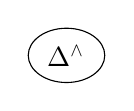
\begin{tikzpicture}[baseline=(n.base)]\node[draw,ellipse,inner sep=3pt] (n) {$\Delta^\wedge$};\end{tikzpicture}}}
\margin{\diagram{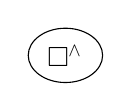
\begin{tikzpicture}[baseline=(n.base)]\node[draw,ellipse,inner sep=3pt] (n) {$\square^\wedge$};\end{tikzpicture}}}
% Hand-drawn arrows are marked blue; typed objects remain plain.
\diagram{\begin{tikzcd}[row sep=small, column sep=small]
\& \& \& \hand{\hat{\Delta}}=\text{(ss. sets)} \arrow[color=blue, dr, "\hand{\xi}"] \& \\
\text{(Ord)} \arrow[color=blue, r, hook] \& \text{(Preord)} \arrow[color=blue, r, hook] \& \text{(Cat)} \arrow[color=blue, ur, "\hand{\alpha}"] \arrow[color=blue, dr, "\hand{\beta}"'] \& \& \text{(Cat)} \\
\& \& \& \hand{\square}=\text{(cub. sets)} \arrow[color=blue, ur, "\hand{\eta}"'] \&
\end{tikzcd}}
where the two last functors, with values in (Cat), are the two obvious
functors, obtained from
\hand{(**)} \hand{$i_A$}: $A^{\hand{\wedge}}\hand{\to}$ (Cat) , \var{\over{a}{$F$}}{\hand{$F$}}{writing over}{ps_134-3_031-v0004} $\hand{\mapsto} A_{/\var{\over{a}{F}}{\hand{F}}{writing over}{ps_134-3_031-v0005}}$
by particularizing to $A=$\hand{$\Delta$} or \hand{$\square$}. As we noticed before, the four first
among these six functors admit left adjoints, but except for the first,
these adjoints are \uline{not} model preserving. The two last functors, and more

%% END SOURCE ps_134-3_031
\ifnum\EditionMode=1
\psapparatusstart
\psentry{ps_134-3_031-v0001}{1}{typed insertion}{\inserted[typed]{$F$:}}{$F$:}{The typed insertion is incorporated at its indicated position; insertion brackets leave the running text.}
\psentry{ps_134-3_031-v0002}{2}{typewriter deletion}{\xout{``model}}{}{The typewriter strikes out this material; it leaves the corrected running text.}
\psentry{ps_134-3_031-v0003}{3}{deletion}{\deleted{\xout{with the}}}{}{The author cancels this material by hand; it leaves the corrected running text.}
\psentry{ps_134-3_031-v0004}{4}{writing over}{\over{a}{$F$}}{\hand{$F$}}{The superposed handwritten reading replaces the underlying reading.}
\psentry{ps_134-3_031-v0005}{5}{writing over}{$\over{a}{F}$}{$\hand{F}$}{The superposed handwritten reading replaces the underlying reading.}
\psapparatusend
\fi
\pssource{ps_134-3_032}{134-3/32}{https://grothendieck.umontpellier.fr/web/viewer.html?file=../134-3.pdf\#page=33}
\psnumber{ps_134-3_032-v0001}{1}
\psnumber{ps_134-3_032-v0002}{2}
\psnumber{ps_134-3_032-v0003}{3}
\psnumber{ps_134-3_032-v0004}{4}
\psnumber{ps_134-3_032-v0005}{5}
\psnumber{ps_134-3_032-v0006}{6}
\psnumber{ps_134-3_032-v0007}{7}
\psnumber{ps_134-3_032-v0008}{8}
\psnumber{ps_134-3_032-v0009}{9}
\psnumber{ps_134-3_032-v0010}{10}
\psnumber{ps_134-3_032-v0011}{11}
%% BEGIN SOURCE ps_134-3_032
% Pursuing Stacks (cotes 134-2 to 134-8): archive cote 134-3, site page 32 (PDF page 33), typescript page 32.
% typescript. Draft compared: ps2.tex:1514-1585.
% AI-transcribed by Claude Opus 5.5 (claude-opus-5-5, adaptive thinking, effort high), Message Batches API, batch ps1 (msgbatch_01Rv5hCaNTtUt4JHx1yqoHPL), 2026-11-12; image review recorded in records/CHECK_DECISIONS_134_3_4.tsv.
\scanpage{134-3/32}
\mspage{32}

generally the functor (**), admit right adjoints, namely the functor

\var{\xout{(Cat)x\allowbreak{}x\allowbreak{}x\allowbreak{}x\allowbreak{}$\hat{A}$x\allowbreak{}x\allowbreak{}x\allowbreak{}x\allowbreak{}x\allowbreak{}x\allowbreak{}ax\allowbreak{}x\allowbreak{}x\allowbreak{}x\allowbreak{}Homx\allowbreak{}}}{}{typewriter deletion}{ps_134-3_032-v0001}

$j_A$: \quad (Cat) $\hand{\longrightarrow} A^{\hand{\wedge}}$ \quad , \quad where \quad $j_A(B) = (\ a \hand{\mapsto} \mathrm{Hom}(A_{/a},B))$ \quad (B $\hand{\in}$ Ob(Cat)
% NOTE: the right edge of the page cuts the end of this line; a handwritten mark (bracket?) stands there
It should be noted that the functors \quad $j_{\hand{\Delta}}$ , $j_{\hand{\square}}$ are \uline{not} the two functors \hand{$\alpha,\beta$}
% Hand-drawn arrows are marked blue; typed objects remain plain.
\diagram{\begin{tikzcd}[row sep=tiny] \& \hand{\Delta}^{\hand{\wedge}} \\ \text{(Cat)} \ar[color=blue, ur] \ar[color=blue, dr] \& \\ \& \hand{\square}^{\hand{\wedge}} \end{tikzcd}} which appear in the diagram above, \quad the latter are associated
to the familiar functors

% Hand-drawn arrows are marked blue; typed objects remain plain.
\margin{(***)} \diagram{\begin{tikzcd}[row sep=tiny] \hand{\Delta} \ar[color=blue, dr] \& \\ \& \text{(Cat)} \\ \hand{\square} \ar[color=blue, ur] \& \end{tikzcd}}

(factoring in fact through (Ord)), associating to every ordered simplex,
or to every multioriented cube, \quad the corresponding 1-skeleton with suitable
orientations on the edges, turning \var{\inserted[typed]{the vertices of}}{the vertices of}{typed insertion}{ps_134-3_032-v0002} this graph into an ordered set; \quad while
the two former are associated to the functors deduced from (**) by restric-%
ting to $A \hand{\subset} A^{\hand{\wedge}}$ , \quad namely
\[ n \hand{\mapsto} \hand{\Delta}\hand{/}\hand{\Delta}_n \]
in the case of \hand{$\Delta$}, \quad and accordingly for \hand{$\square$}. \quad The values of these functors,
contrarily to the two preceding ones, \quad are \uline{infinite} categories, \quad and they
cannot be described by \var{\inserted{(i.e. ``are'' not)}}{\hand{(i.e. ``are'' not)}}{insertion}{ps_134-3_032-v0003} (pre)ordered sets. \quad If however we had defined
the categories \hand{$\Delta$} , \hand{$\square$} \quad in terms of iterated boundary operations only, \quad exclu%
% NOTE: the right edge of the page cuts the end of the line after "exclu"
ding the degeneracy operations (which, \quad I feel, \quad are not really needed for
turning \hand{$\Delta^\wedge$} and \hand{$\square^\wedge$} into model\var{\over{ato}{ize}}{\hand{ize}}{writing over}{ps_134-3_032-v0004}rs), \quad we would get indeed \uline{finite} ordered
sets, \quad namely the full combinatorial simplices or cubes, \var{\inserted[typed]{each one}}{each one}{typed insertion}{ps_134-3_032-v0005} embodied by the
ordered set of all it's facettes of all possible dimensions.

Contrarily to what happens with the functors \hand{$\alpha$, $\beta$}, \quad I feel that for
the two functors \hand{$\xi,\eta$} in opposite direction, \quad not only are they model pre-%
serving, \quad but the \var{\inserted[typed]{right}}{right}{typed insertion}{ps_134-3_032-v0006} adjoint functors \quad $j_{\hand{\Delta}}$ , $j_{\hand{\square}}$ must be model preserving too,
and we will have to come back upon this in a more general context.

We could amplify and unify somewhat the previous diagram of modelizers,
by introducing multicomplexes, \quad which after all can be as well ``mixed''
namely partly semisimplicial, \quad partly cubical. \quad Namely, \quad we may introduce
the would-be \var{\inserted{``}}{\hand{``}}{insertion}{ps_134-3_032-v0007}test categories'' \hand{(30)}
\[ (\hand{\Delta})^p \hand{\times} (\hand{\Delta})^q = T_{p,q} \qquad (p,q \hand{\in} \underline{N} \ , \quad p+q \var{\over{>}{\geq}}{\hand{\geq}}{writing over}{ps_134-3_032-v0008} 1) \]
giving rise to the category \quad $T^{\hand{\wedge}}_{p,q}$ \var{\deleted{\unsure{x}}}{}{deletion}{ps_134-3_032-v0009} \quad of (p,q)-multicomplexes (p times
simplicial, q times cubical). \quad \var{\xout{The}}{}{typewriter deletion}{ps_134-3_032-v0010} We have a natural functor (generalizing
the functors (xxx))
\[ T_{p,q} \hand{\longrightarrow} \text{(Ord)} \hand{(} \hand{\hookrightarrow} \text{(Cat)} \hand{)} \ , \]
associating to a system of p standart simplices and q standart cubes
(of variable dimensions), \quad the \uline{product} of the p+q associated ordered sets.
We get this way a functor
\[ \hand{\alpha_{p,q}} \ \var{\deleted{\hand{\illegible{1}_{p,q}}}}{}{deletion}{ps_134-3_032-v0011} : \text{(Cat)} \hand{\longrightarrow} T^{\hand{\wedge}}_{p,q} \]

%% END SOURCE ps_134-3_032
\ifnum\EditionMode=1
\psapparatusstart
\psentry{ps_134-3_032-v0001}{1}{typewriter deletion}{\xout{(Cat)x\allowbreak{}x\allowbreak{}x\allowbreak{}x\allowbreak{}$\hat{A}$x\allowbreak{}x\allowbreak{}x\allowbreak{}x\allowbreak{}x\allowbreak{}x\allowbreak{}ax\allowbreak{}x\allowbreak{}x\allowbreak{}x\allowbreak{}Homx\allowbreak{}}}{}{The typewriter strikes out this material; it leaves the corrected running text.}
\psentry{ps_134-3_032-v0002}{2}{typed insertion}{\inserted[typed]{the vertices of}}{the vertices of}{The typed insertion is incorporated at its indicated position; insertion brackets leave the running text.}
\psentry{ps_134-3_032-v0003}{3}{insertion}{\inserted{(i.e. ``are'' not)}}{\hand{(i.e. ``are'' not)}}{The handwritten insertion is incorporated at its indicated position; insertion brackets leave the running text.}
\psentry{ps_134-3_032-v0004}{4}{writing over}{\over{ato}{ize}}{\hand{ize}}{The superposed handwritten reading replaces the underlying reading.}
\psentry{ps_134-3_032-v0005}{5}{typed insertion}{\inserted[typed]{each one}}{each one}{The typed insertion is incorporated at its indicated position; insertion brackets leave the running text.}
\psentry{ps_134-3_032-v0006}{6}{typed insertion}{\inserted[typed]{right}}{right}{The typed insertion is incorporated at its indicated position; insertion brackets leave the running text.}
\psentry{ps_134-3_032-v0007}{7}{insertion}{\inserted{``}}{\hand{``}}{The handwritten insertion is incorporated at its indicated position; insertion brackets leave the running text.}
\psentry{ps_134-3_032-v0008}{8}{writing over}{$\over{>}{\geq}$}{$\hand{\geq}$}{The superposed handwritten reading replaces the underlying reading.}
\psentry{ps_134-3_032-v0009}{9}{deletion}{\deleted{\unsure{x}}}{}{The author cancels this material by hand; it leaves the corrected running text.}
\psentry{ps_134-3_032-v0010}{10}{typewriter deletion}{\xout{The}}{}{The typewriter strikes out this material; it leaves the corrected running text.}
\psentry{ps_134-3_032-v0011}{11}{deletion}{$\deleted{\hand{\illegible{1}_{p,q}}}$}{}{The author cancels this material by hand; it leaves the corrected running text.}
\psapparatusend
\fi
\pssource{ps_134-3_033}{134-3/33}{https://grothendieck.umontpellier.fr/web/viewer.html?file=../134-3.pdf\#page=34}
\psnumber{ps_134-3_033-v0001}{1}
\psnumber{ps_134-3_033-v0002}{2}
\psnumber{ps_134-3_033-v0003}{3}
\psnumber{ps_134-3_033-v0004}{4}
\psnumber{ps_134-3_033-v0005}{5}
\psnumber{ps_134-3_033-v0006}{6}
\psnumber{ps_134-3_033-v0007}{7}
\psnumber{ps_134-3_033-v0008}{8}
\psnumber{ps_134-3_033-v0009}{9}
%% BEGIN SOURCE ps_134-3_033
% Pursuing Stacks (cotes 134-2 to 134-8): archive cote 134-3, site page 33 (PDF page 34), typescript page 33.
% typescript. Draft compared: ps2.tex:1567-1638.
% AI-transcribed by Claude Opus 5.5 (claude-opus-5-5, adaptive thinking, effort high), Message Batches API, batch ps1 (msgbatch_01Rv5hCaNTtUt4JHx1yqoHPL), 2026-11-12; image review recorded in records/CHECK_DECISIONS_134_3_4.tsv.
\scanpage{134-3/33}
\mspage{\hand{33}}
which presumably (as I already felt yesterday, cf first lines p.24) is not
any less model-preserving than the functors $\hand{\alpha},\hand{\beta}$ it generalizes.  Of course,
taking A = $T_{p,q}$ above,  we equally get a natural functor
\[ \hand{i_{p,q}} : T^{\hand{\wedge}}_{p,q} \hand{\longrightarrow} (\mathrm{Cat}) \]
\margin{\diagram{\begin{tikzpicture}[x=1em,y=1em]\draw[->] (1.7,0)--(.2,0) .. controls (0,0) and (0,.2) .. (0,.5)--(0,2.1);\end{tikzpicture}}} admitting a right adjoint \var{\inserted{$j_{p,q}$}}{\hand{$j_{p,q}$}}{insertion}{ps_134-3_033-v0001}, and both functors I feel must be model preser-%
ving.

\var{\over{\unsure{26}}{29}}{\hand{29}}{writing over}{ps_134-3_033-v0002}.  It is time now to elaborate a little upon the notion of a test catego-%
ry,  within the context of modelizers.  Let A be a small category,  and
consider  the functor (**)
\margin{\diagram{\begin{tikzpicture}[x=1em,y=1em]\draw[->] (1.7,0)--(.2,0) .. controls (0,0) and (0,-.2) .. (0,-.5)--(0,-2.8);\end{tikzpicture}}} (**) \[ \hand{i}_{A} : A^{\hand{\wedge}} \hand{\longrightarrow} (\mathrm{Cat}) \quad , \quad F \hand{\mapsto} A_{/F} \quad , \]
Whenever we have a functor \var{\inserted[typed]{i:}}{i:}{typed insertion}{ps_134-3_033-v0003} $M \hand{\to} M'$,  when $M'$ is equipped with a $W'$ turning
it into a modelizer,  there is (if any) \var{\xout{xx}}{}{typewriter deletion}{ps_134-3_033-v0004} just one $W \hand{\subset} \mathrm{F}\var{\over{l}{l}}{\hand{l}}{writing over}{ps_134-3_033-v0005}(M)$ turning M into
a modelizer and i into a morphism of such,  namely $W = i_{\mathrm{F}\var{\over{l}{l}}{\hand{l}}{writing over}{ps_134-3_033-v0006}}^{-1}(W')$.  In any
case,  we may define W (``weak equivalences'') by this formula,  and get a
functor
\[ W^{-1}M \hand{\longrightarrow} W'^{-1}M' \quad , \]
which is an equivalence iff (M,W) is indeed a modelizer and i model\var{\xout{\unsure{s}}}{}{typewriter deletion}{ps_134-3_033-v0007}preser-%
ving.  We may say shortly that i: $M \hand{\to} M'$ is model preserving,  even without
any W given beforehand.  Now coming back to the situation  (**),  the under-%
standing yesterday was to call A a \uline{test} \uline{category} ,  to express that the
canonical functor (**) is model preserving. \hand{(}In any case,  unless otherwise
specified by the context, we will refer to arrows in $A\hand{^{\wedge}}$ which are transfor-%
med into weak equivalences of (Cat)  as ``\uline{weak equivalences}''.\hand{)} It may well
turn out,  by the way,  that we will have to restrict somewhat still the
notion of a test category.

\margin{\diagram{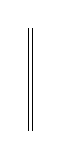
\begin{tikzpicture}[x=1em,y=1em]\draw (0,0)--(0,-3.7);\draw (.17,0)--(.17,-3.7);\end{tikzpicture}}} In any case,  \uline{the basic modelizer,}  \uline{in this whole approach to homotopy}
\uline{models,}  \uline{is by no means the category} (Ss sets)  (however handy)  \uline{or the}
\uline{category} (Spaces)  (howeve\var{\xout{\unsure{t}}}{}{typewriter deletion}{ps_134-3_033-v0008}r appealing to topological intuition),  \uline{but the}
\uline{category} (Cat) \uline{of} \uline{``all''} (small) \uline{categories.}  In this set-up,  the category
(Hot) is most suitably defined as the category of fractions of (Cat) with
respect to ``weak equivalences''.  These in turn are most suitably defined
in cohomological terms,  via the corresponding notion for topoi  -  namely
a morphism of topoi
\[ f:\ X \hand{\longrightarrow} X' \]
is a ``weak equivalence'' or homotopy equivalence,  iff for every locally
constant sheaf $F'$ on $X'$, the maps
\[ H^{i}(X',F') \hand{\to} H^{i}(X,f^{-1}(F')) \]
are isomorphisms whenever defined  -  namely for i=0,  for i=1 if moreover
$F'$ is endowed with a group structure,  and for any i if $F'$ is moreover
commutative\var{\xout{t}}{}{typewriter deletion}{ps_134-3_033-v0009} (\uline{Criterion} \uline{of} \uline{Artin-Mazur}).  Accordingly,  a functor

%% END SOURCE ps_134-3_033
\ifnum\EditionMode=1
\psapparatusstart
\psentry{ps_134-3_033-v0001}{1}{insertion}{\inserted{$j_{p,q}$}}{\hand{$j_{p,q}$}}{The handwritten insertion is incorporated at its indicated position; insertion brackets leave the running text.}
\psentry{ps_134-3_033-v0002}{2}{writing over}{\over{\unsure{26}}{29}}{\hand{29}}{The superposed handwritten reading replaces the underlying reading.}
\psentry{ps_134-3_033-v0003}{3}{typed insertion}{\inserted[typed]{i:}}{i:}{The typed insertion is incorporated at its indicated position; insertion brackets leave the running text.}
\psentry{ps_134-3_033-v0004}{4}{typewriter deletion}{\xout{xx}}{}{The typewriter strikes out this material; it leaves the corrected running text.}
\psentry{ps_134-3_033-v0005}{5}{writing over}{$\over{l}{l}$}{$\hand{l}$}{The superposed handwritten reading replaces the underlying reading.}
\psentry{ps_134-3_033-v0006}{6}{writing over}{$\over{l}{l}$}{$\hand{l}$}{The superposed handwritten reading replaces the underlying reading.}
\psentry{ps_134-3_033-v0007}{7}{typewriter deletion}{\xout{\unsure{s}}}{}{The typewriter strikes out this material; it leaves the corrected running text.}
\psentry{ps_134-3_033-v0008}{8}{typewriter deletion}{\xout{\unsure{t}}}{}{The typewriter strikes out this material; it leaves the corrected running text.}
\psentry{ps_134-3_033-v0009}{9}{typewriter deletion}{\xout{t}}{}{The typewriter strikes out this material; it leaves the corrected running text.}
\psapparatusend
\fi
\pssource{ps_134-3_034}{134-3/34}{https://grothendieck.umontpellier.fr/web/viewer.html?file=../134-3.pdf\#page=35}
\psnumber{ps_134-3_034-v0001}{1}
\psnumber{ps_134-3_034-v0002}{2}
\psnumber{ps_134-3_034-v0003}{3}
\psnumber{ps_134-3_034-v0004}{4}
\psnumber{ps_134-3_034-v0005}{5}
\psnumber{ps_134-3_034-v0006}{6}
\psnumber{ps_134-3_034-v0007}{7}
\psnumber{ps_134-3_034-v0008}{8}
\psnumber{ps_134-3_034-v0009}{9}
\psnumber{ps_134-3_034-v0010}{10}
\psnumber{ps_134-3_034-v0011}{11}
\psnumber{ps_134-3_034-v0012}{12}
\psnumber{ps_134-3_034-v0013}{13}
\psnumber{ps_134-3_034-v0014}{14}
\psnumber{ps_134-3_034-v0015}{15}
\psnumber{ps_134-3_034-v0016}{16}
\psnumber{ps_134-3_034-v0017}{17}
\psnumber{ps_134-3_034-v0018}{18}
\psnumber{ps_134-3_034-v0019}{19}
\psnumber{ps_134-3_034-v0020}{20}
\psnumber{ps_134-3_034-v0021}{21}
\psnumber{ps_134-3_034-v0022}{22}
\psnumber{ps_134-3_034-v0023}{23}
\psnumber{ps_134-3_034-v0024}{24}
\psnumber{ps_134-3_034-v0025}{25}
\psnumber{ps_134-3_034-v0026}{26}
\psnumber{ps_134-3_034-v0027}{27}
\psnumber{ps_134-3_034-v0028}{28}
\psnumber{ps_134-3_034-v0029}{29}
\psnumber{ps_134-3_034-v0030}{30}
\psnumber{ps_134-3_034-v0031}{31}
%% BEGIN SOURCE ps_134-3_034
% Pursuing Stacks (cotes 134-2 to 134-8): archive cote 134-3, site page 34 (PDF page 35), typescript page 34.
% typescript. Draft compared: ps2.tex:1621-1693.
% AI-transcribed by Claude Opus 5.5 (claude-opus-5-5, adaptive thinking, effort high), Message Batches API, batch ps1 (msgbatch_01Rv5hCaNTtUt4JHx1yqoHPL), 2026-11-12; image review recorded in records/CHECK_DECISIONS_134_3_4.tsv.
\scanpage{134-3/34}
\mspage{\hand{34}}
\[ f\colon A \hand{\longrightarrow} A' \]
between small categories (or categories which are essentially small, name-%
ly equivalent to small categories) is called a weak equivalence, iff the
corresponding morphism of topoi
\[ f\hand{\hat{}}\colon \var{\deleted{\illegible{1}}}{}{deletion}{ps_134-3_034-v0001}\ A\hand{\hat{}} \hand{\to} A'\hand{\hat{}} \]
is a weak equivalence.

Coming back to test categories A, which allow to construct the cor-%
responding modelizers $A\hand{\hat{}}$, our point of view here is rather that \uline{the test
categories are each just as good \var{\inserted{one}}{\hand{one}}{insertion}{ps_134-3_034-v0002} as the other\var{\deleted{s}}{}{deletion}{ps_134-3_034-v0003}}, and \hand{$\Delta$} just as good as
\hand{$\Box$} or any of the $T_{p,q}$ and not any better ! Maybe it's the one though which
turns out the most economical for computational use, the nerve functor
(Cat)$\hand{\to}$ \hand{$\Delta$}$\hand{\hat{}}$ being still the neatest known of all \var{\inserted[typed]{model preserving}}{model preserving}{typed insertion}{ps_134-3_034-v0004} embeddings of (Cat) into
categories $A\hand{\hat{}}$ defined by modelizers.\hand{$^{(31)}$.} Another \var{\inserted[typed]{point}}{point}{typed insertion}{ps_134-3_034-v0005}, still more important \var{\deleted{\xout{point}}}{}{deletion}{ps_134-3_034-v0006}
it seems to me, is that the natural functor
\[ \text{(Topoi)} \hand{\longrightarrow} \text{Pro(Hot)} \]
defined by the \hand{\v{}}Cech-Cartier-Verdier process, and which allows for another
description of weak equivalences of topoi\hand{,} \var{\inserted{namely}}{\hand{namely}}{insertion}{ps_134-3_034-v0007} as those made invertible by this
functor, are directly defined via semi-simplicial structures or simplicial
structures (of the type ``nerve of a covering'')\hand{$^{(32)}$.}

Modelizers of the type $A\hand{\hat{}}$, with A a test category, surely deserve
a name - lets call them \uline{elementary} \uline{modelizers}, as they correspond to \var{\xout{xx}}{}{typewriter deletion}{ps_134-3_034-v0008}
the case of an ``elementary'' or ``trivial'' algebraic structure species,
whose set-theoretical realizations can be expressed as just \uline{any} functors
\[ A^{o} \hand{\longrightarrow} \text{(Sets)} , \]
without any exactness condition of any kind\var{\over{,}{;}}{\hand{;}}{writing over}{ps_134-3_034-v0009} in other words they can
be viewed as just diagrams of sets of a specified type, with specified
commutativity relations. A somewhat ambitious question maybe is whether
on such a category \var{\inserted[typed]{$M=$}}{$M=$}{typed insertion}{ps_134-3_034-v0010} $A\hand{\hat{}}$, namely an elementary modelizer, there \var{\inserted[typed]{cannot}}{cannot}{typed insertion}{ps_134-3_034-v0011} \var{\xout{xxx}}{}{typewriter deletion}{ps_134-3_034-v0012} exist
\var{\inserted[typed]{any}}{any}{typed insertion}{ps_134-3_034-v0013} \var{\xout{xx}}{}{typewriter deletion}{ps_134-3_034-v0014}other modelizing structure. In any case, the one we got is intrinsicly
determined in terms of M, which is a topos, by the prescription that
an arrow $f\colon a \hand{\to} b$ within M is a weak equivalence if and only if the
corresponding morphism \var{\inserted[typed]{for}}{for}{typed insertion}{ps_134-3_034-v0015} \var{\xout{xx}}{}{typewriter deletion}{ps_134-3_034-v0016} the induced topoi $M_{/a}$ and $M/_{b}$ is a weak equiva-%
lence (in terms of the Artin-Mazur criterion \var{\deleted{\unsure{above section}}}{}{deletion}{ps_134-3_034-v0017} \var{\inserted{of section 17}}{\hand{of section 17}}{insertion}{ps_134-3_034-v0018}\hand{)}.

\var{\xout{Let}}{}{typewriter deletion}{ps_134-3_034-v0019} A more crucial question I feel is whether the \var{\inserted[typed]{right}}{right}{typed insertion}{ps_134-3_034-v0020} adjoint functor
$j_{A}$ to $i_{A}$ in (**) (cf. \var{\deleted{\illegible{1}}}{}{deletion}{ps_134-3_034-v0021} \var{\inserted{section 28)}}{\hand{section 28)}}{insertion}{ps_134-3_034-v0022} is equally model preserving, whenever A is a
test category. This, as we have seen, is \uline{not} automatic\unsure{,} whenever we
have a model preserving functor between modelizers, \var{\inserted{whenever}}{\hand{whenever}}{insertion}{ps_134-3_034-v0023} this functor admit\var{\over{ting}{s}}{\hand{s}}{writing over}{ps_134-3_034-v0024}
an adjoint functor. In \var{\inserted[typed]{more}}{more}{typed insertion}{ps_134-3_034-v0025} \var{\inserted{general}}{\hand{general}}{insertion}{ps_134-3_034-v0026} \var{\xout{xxxxxxx}}{}{typewriter deletion}{ps_134-3_034-v0027} terms \var{\xout{and more}}{}{typewriter deletion}{ps_134-3_034-v0028} still, let
% Hand-drawn arrows are marked blue; typed objects remain plain.
\diagram{\begin{tikzcd} M \ar[color=blue, r, shift left, "\hand{i}"] \& M' \ar[color=blue, l, shift left, "\hand{j}"] \end{tikzcd}}
\margin{\diagram{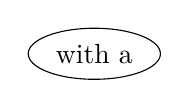
\begin{tikzpicture}[baseline=(n.base)]\node[draw,ellipse,inner sep=3pt] (n) {with a};\end{tikzpicture}}}
be a pair of adjoint functors, with M,M' endowed \var{\deleted{with two}}{}{deletion}{ps_134-3_034-v0029} \var{\inserted{with a}}{\hand{with a}}{insertion}{ps_134-3_034-v0030} \uline{``saturated''} \var{\deleted{sets}}{}{deletion}{ps_134-3_034-v0031}

%% END SOURCE ps_134-3_034
\ifnum\EditionMode=1
\psapparatusstart
\psentry{ps_134-3_034-v0001}{1}{deletion}{$\deleted{\illegible{1}}$}{}{The author cancels this material by hand; it leaves the corrected running text.}
\psentry{ps_134-3_034-v0002}{2}{insertion}{\inserted{one}}{\hand{one}}{The handwritten insertion is incorporated at its indicated position; insertion brackets leave the running text.}
\psentry{ps_134-3_034-v0003}{3}{deletion}{\deleted{s}}{}{The author cancels this material by hand; it leaves the corrected running text.}
\psentry{ps_134-3_034-v0004}{4}{typed insertion}{\inserted[typed]{model preserving}}{model preserving}{The typed insertion is incorporated at its indicated position; insertion brackets leave the running text.}
\psentry{ps_134-3_034-v0005}{5}{typed insertion}{\inserted[typed]{point}}{point}{The typed insertion is incorporated at its indicated position; insertion brackets leave the running text.}
\psentry{ps_134-3_034-v0006}{6}{deletion}{\deleted{\xout{point}}}{}{The author cancels this material by hand; it leaves the corrected running text.}
\psentry{ps_134-3_034-v0007}{7}{insertion}{\inserted{namely}}{\hand{namely}}{The handwritten insertion is incorporated at its indicated position; insertion brackets leave the running text.}
\psentry{ps_134-3_034-v0008}{8}{typewriter deletion}{\xout{xx}}{}{The typewriter strikes out this material; it leaves the corrected running text.}
\psentry{ps_134-3_034-v0009}{9}{writing over}{\over{,}{;}}{\hand{;}}{The superposed handwritten reading replaces the underlying reading.}
\psentry{ps_134-3_034-v0010}{10}{typed insertion}{\inserted[typed]{$M=$}}{$M=$}{The typed insertion is incorporated at its indicated position; insertion brackets leave the running text.}
\psentry{ps_134-3_034-v0011}{11}{typed insertion}{\inserted[typed]{cannot}}{cannot}{The typed insertion is incorporated at its indicated position; insertion brackets leave the running text.}
\psentry{ps_134-3_034-v0012}{12}{typewriter deletion}{\xout{xxx}}{}{The typewriter strikes out this material; it leaves the corrected running text.}
\psentry{ps_134-3_034-v0013}{13}{typed insertion}{\inserted[typed]{any}}{any}{The typed insertion is incorporated at its indicated position; insertion brackets leave the running text.}
\psentry{ps_134-3_034-v0014}{14}{typewriter deletion}{\xout{xx}}{}{The typewriter strikes out this material; it leaves the corrected running text.}
\psentry{ps_134-3_034-v0015}{15}{typed insertion}{\inserted[typed]{for}}{for}{The typed insertion is incorporated at its indicated position; insertion brackets leave the running text.}
\psentry{ps_134-3_034-v0016}{16}{typewriter deletion}{\xout{xx}}{}{The typewriter strikes out this material; it leaves the corrected running text.}
\psentry{ps_134-3_034-v0017}{17}{deletion}{\deleted{\unsure{above section}}}{}{The author cancels this material by hand; it leaves the corrected running text.}
\psentry{ps_134-3_034-v0018}{18}{insertion}{\inserted{of section 17}}{\hand{of section 17}}{The handwritten insertion is incorporated at its indicated position; insertion brackets leave the running text.}
\psentry{ps_134-3_034-v0019}{19}{typewriter deletion}{\xout{Let}}{}{The typewriter strikes out this material; it leaves the corrected running text.}
\psentry{ps_134-3_034-v0020}{20}{typed insertion}{\inserted[typed]{right}}{right}{The typed insertion is incorporated at its indicated position; insertion brackets leave the running text.}
\psentry{ps_134-3_034-v0021}{21}{deletion}{\deleted{\illegible{1}}}{}{The author cancels this material by hand; it leaves the corrected running text.}
\psentry{ps_134-3_034-v0022}{22}{insertion}{\inserted{section 28)}}{\hand{section 28)}}{The handwritten insertion is incorporated at its indicated position; insertion brackets leave the running text.}
\psentry{ps_134-3_034-v0023}{23}{insertion}{\inserted{whenever}}{\hand{whenever}}{The handwritten insertion is incorporated at its indicated position; insertion brackets leave the running text.}
\psentry{ps_134-3_034-v0024}{24}{writing over}{\over{ting}{s}}{\hand{s}}{The superposed handwritten reading replaces the underlying reading.}
\psentry{ps_134-3_034-v0025}{25}{typed insertion}{\inserted[typed]{more}}{more}{The typed insertion is incorporated at its indicated position; insertion brackets leave the running text.}
\psentry{ps_134-3_034-v0026}{26}{insertion}{\inserted{general}}{\hand{general}}{The handwritten insertion is incorporated at its indicated position; insertion brackets leave the running text.}
\psentry{ps_134-3_034-v0027}{27}{typewriter deletion}{\xout{xxxxxxx}}{}{The typewriter strikes out this material; it leaves the corrected running text.}
\psentry{ps_134-3_034-v0028}{28}{typewriter deletion}{\xout{and more}}{}{The typewriter strikes out this material; it leaves the corrected running text.}
\psentry{ps_134-3_034-v0029}{29}{deletion}{\deleted{with two}}{}{The author cancels this material by hand; it leaves the corrected running text.}
\psentry{ps_134-3_034-v0030}{30}{insertion}{\inserted{with a}}{\hand{with a}}{The handwritten insertion is incorporated at its indicated position; insertion brackets leave the running text.}
\psentry{ps_134-3_034-v0031}{31}{deletion}{\deleted{sets}}{}{The author cancels this material by hand; it leaves the corrected running text.}
\psapparatusend
\fi
\pssource{ps_134-3_035}{134-3/35}{https://grothendieck.umontpellier.fr/web/viewer.html?file=../134-3.pdf\#page=36}
\psnumber{ps_134-3_035-v0001}{1}
\psnumber{ps_134-3_035-v0002}{2}
\psnumber{ps_134-3_035-v0003}{3}
\psnumber{ps_134-3_035-v0004}{4}
\psnumber{ps_134-3_035-v0005}{5}
\psnumber{ps_134-3_035-v0006}{6}
\psnumber{ps_134-3_035-v0007}{7}
\psnumber{ps_134-3_035-v0008}{8}
\psnumber{ps_134-3_035-v0009}{9}
\psnumber{ps_134-3_035-v0010}{10}
\psnumber{ps_134-3_035-v0011}{11}
\psnumber{ps_134-3_035-v0012}{12}
\psnumber{ps_134-3_035-v0013}{13}
\psnumber{ps_134-3_035-v0014}{14}
\psnumber{ps_134-3_035-v0015}{15}
\psnumber{ps_134-3_035-v0016}{16}
\psnumber{ps_134-3_035-v0017}{17}
\psnumber{ps_134-3_035-v0018}{18}
\psnumber{ps_134-3_035-v0019}{19}
\psnumber{ps_134-3_035-v0020}{20}
\psnumber{ps_134-3_035-v0021}{21}
%% BEGIN SOURCE ps_134-3_035
% Pursuing Stacks (cotes 134-2 to 134-8): archive cote 134-3, site page 35 (PDF page 36), typescript page 35.
% typescript. Draft compared: ps2.tex:1674-1745.
% AI-transcribed by Claude Opus 5.5 (claude-opus-5-5, adaptive thinking, effort high), Message Batches API, batch ps1 (msgbatch_01Rv5hCaNTtUt4JHx1yqoHPL), 2026-11-12; image review recorded in records/CHECK_DECISIONS_134_3_4.tsv.
\scanpage{134-3/35}
\mspage{35}
set of arrows W,W'. Then the following are equivalent:

a) $i(W)\hand{\subset} W'$, $j(W')\hand{\subset} W$, and the two corresponding functors
\[ W^{-1}M \hand{\rightleftarrows} W'^{-1}M' \]
are quasi-inverse of each other, the adjunction morphisms between
them being deduced from the corresponding adjunction morphisms
for the pair (i,j).

b) $W=i^{-1}(W')$, and for every $a'\hand{\in} M'$, the adjunction morphism
\[ \var{\xout{ax}}{}{typewriter deletion}{ps_134-3_035-v0001} \quad i\var{\over{j}{j}}{\hand{j}}{writing over}{ps_134-3_035-v0002}(a')\hand{\to} a' \]
is in W'.

b') dual to b), with roles of M and M' reversed.

In the situation we are interested in here, $M = A\hand{\hat{}}$\hand{/}and $M' = $ (Cat),
we know already $W=i^{-1}(W')$ by definition, and hence all we have to see is
w\hand{h}ether for any \var{\inserted{[small]}}{\hand{[small]}}{insertion}{ps_134-3_035-v0003} category B, the functor
\[ \text{(T)} \qquad \var{\xout{B}}{}{typewriter deletion}{ps_134-3_035-v0004} \quad \var{\over{i}{i}}{\hand{i}}{writing over}{ps_134-3_035-v0005}_A \var{\over{j}{j}}{\hand{j}}{writing over}{ps_134-3_035-v0006}_A(B) \hand{\longrightarrow} B \]
is a \var{\xout{quasi}}{}{typewriter deletion}{ps_134-3_035-v0007} \var{\inserted[typed]{weak}}{weak}{typed insertion}{ps_134-3_035-v0008} equivalence. This alone will imply that not only $i_{W,W'}$ , but
equally $j_{W',W}$ is an equivalence, and that the two are quasi-inverse of
each other. (NB even without assuming beforehand that W \var{\xout{is}}{}{typewriter deletion}{ps_134-3_035-v0009}\var{\inserted[typed]{W' are}}{W' are}{typed insertion}{ps_134-3_035-v0010} saturated ,
b) (say) implies b') and a), \var{\xout{and}}{}{typewriter deletion}{ps_134-3_035-v0011} provided we assume on W' the very mild
saturation condition that for composable arrows $u',v'$, if two among $u',v'$,
$v'u'$ are in W', so is the third; \var{\xout{moreover,}}{}{typewriter deletion}{ps_134-3_035-v0012} if we suppose moreover that
M' is actually saturated namely made up with all arrows made invertible by
$M'\hand{\to} W'^{-1}M'$, then condition b) implies that M is saturated too - which
insures that if (M',W') is modelizing, so is (M,W).\hand{)}

It is not clear to me whether for every test category A, the stronger
condition (T) above is necessarily satisfied. \var{\xout{It}}{}{typewriter deletion}{ps_134-3_035-v0013} \var{\inserted[typed]{This condition essentially}}{This condition essentially}{typed insertion}{ps_134-3_035-v0014} means that for any homo-%
topy type, defined in terms of an arbitrary element B in (Cat) namely
a category B, we get a description of this homotopy type \var{\over{by}{by}}{\hand{by}}{writing over}{ps_134-3_035-v0015} an object of
the elementary modelizer $A\hand{\hat{}}$,\hand{|}by merely taking $j_A(B)$. This condition seems
sufficiently appealing to me, for reinforcing adcordingly the notion of
atest-category A, and of an elementary normalizer $A\hand{\hat{}}$, in case it should
turn out to be actually stronger\hand{(${}^{33}$)}. Of course, any category equivalent to
an elementary modelizer $A\hand{\hat{}}$\hand{/}will be equally called by the same name. It \var{\xout{should}}{}{typewriter deletion}{ps_134-3_035-v0016}
should appear in \var{\xout{the}}{}{typewriter deletion}{ps_134-3_035-v0017} due course whether this is indeed the better suited
notion. One point in it\hand{'}s favor \var{\xout{though}}{}{typewriter deletion}{ps_134-3_035-v0018}\var{\inserted[typed]{already}}{already}{typed insertion}{ps_134-3_035-v0019} is that it \var{\over{app}{app}}{\hand{app}}{writing over}{ps_134-3_035-v0020}ears a lot more
concrete.

Another natural question, suggested by the use of simplicial or cubi-%
cal multicomplexes, is whether the product of two test categories is again
a test category - which might furnish us with a way to compare \var{\xout{the}}{}{typewriter deletion}{ps_134-3_035-v0021} direct-%
ly the description of (Hot) by the associated elementary modelizers, with\hand{out}

%% END SOURCE ps_134-3_035
\ifnum\EditionMode=1
\psapparatusstart
\psentry{ps_134-3_035-v0001}{1}{typewriter deletion}{$\xout{ax}$}{}{The typewriter strikes out this material; it leaves the corrected running text.}
\psentry{ps_134-3_035-v0002}{2}{writing over}{$\over{j}{j}$}{$\hand{j}$}{The superposed handwritten reading replaces the underlying reading.}
\psentry{ps_134-3_035-v0003}{3}{insertion}{\inserted{[small]}}{\hand{[small]}}{The handwritten insertion is incorporated at its indicated position; insertion brackets leave the running text.}
\psentry{ps_134-3_035-v0004}{4}{typewriter deletion}{$\xout{B}$}{}{The typewriter strikes out this material; it leaves the corrected running text.}
\psentry{ps_134-3_035-v0005}{5}{writing over}{$\over{i}{i}$}{$\hand{i}$}{The superposed handwritten reading replaces the underlying reading.}
\psentry{ps_134-3_035-v0006}{6}{writing over}{$\over{j}{j}$}{$\hand{j}$}{The superposed handwritten reading replaces the underlying reading.}
\psentry{ps_134-3_035-v0007}{7}{typewriter deletion}{\xout{quasi}}{}{The typewriter strikes out this material; it leaves the corrected running text.}
\psentry{ps_134-3_035-v0008}{8}{typed insertion}{\inserted[typed]{weak}}{weak}{The typed insertion is incorporated at its indicated position; insertion brackets leave the running text.}
\psentry{ps_134-3_035-v0009}{9}{typewriter deletion}{\xout{is}}{}{The typewriter strikes out this material; it leaves the corrected running text.}
\psentry{ps_134-3_035-v0010}{10}{typed insertion}{\inserted[typed]{W' are}}{W' are}{The typed insertion is incorporated at its indicated position; insertion brackets leave the running text.}
\psentry{ps_134-3_035-v0011}{11}{typewriter deletion}{\xout{and}}{}{The typewriter strikes out this material; it leaves the corrected running text.}
\psentry{ps_134-3_035-v0012}{12}{typewriter deletion}{\xout{moreover,}}{}{The typewriter strikes out this material; it leaves the corrected running text.}
\psentry{ps_134-3_035-v0013}{13}{typewriter deletion}{\xout{It}}{}{The typewriter strikes out this material; it leaves the corrected running text.}
\psentry{ps_134-3_035-v0014}{14}{typed insertion}{\inserted[typed]{This condition essentially}}{This condition essentially}{The typed insertion is incorporated at its indicated position; insertion brackets leave the running text.}
\psentry{ps_134-3_035-v0015}{15}{writing over}{\over{by}{by}}{\hand{by}}{The superposed handwritten reading replaces the underlying reading.}
\psentry{ps_134-3_035-v0016}{16}{typewriter deletion}{\xout{should}}{}{The typewriter strikes out this material; it leaves the corrected running text.}
\psentry{ps_134-3_035-v0017}{17}{typewriter deletion}{\xout{the}}{}{The typewriter strikes out this material; it leaves the corrected running text.}
\psentry{ps_134-3_035-v0018}{18}{typewriter deletion}{\xout{though}}{}{The typewriter strikes out this material; it leaves the corrected running text.}
\psentry{ps_134-3_035-v0019}{19}{typed insertion}{\inserted[typed]{already}}{already}{The typed insertion is incorporated at its indicated position; insertion brackets leave the running text.}
\psentry{ps_134-3_035-v0020}{20}{writing over}{\over{app}{app}}{\hand{app}}{The superposed handwritten reading replaces the underlying reading.}
\psentry{ps_134-3_035-v0021}{21}{typewriter deletion}{\xout{the}}{}{The typewriter strikes out this material; it leaves the corrected running text.}
\psapparatusend
\fi
\pssource{ps_134-3_036}{134-3/36}{https://grothendieck.umontpellier.fr/web/viewer.html?file=../134-3.pdf\#page=37}
\psnumber{ps_134-3_036-v0001}{1}
\psnumber{ps_134-3_036-v0002}{2}
\psnumber{ps_134-3_036-v0003}{3}
\psnumber{ps_134-3_036-v0004}{4}
\psnumber{ps_134-3_036-v0005}{5}
\psnumber{ps_134-3_036-v0006}{6}
\psnumber{ps_134-3_036-v0007}{7}
\psnumber{ps_134-3_036-v0008}{8}
\psnumber{ps_134-3_036-v0009}{9}
\psnumber{ps_134-3_036-v0010}{10}
\psnumber{ps_134-3_036-v0011}{11}
%% BEGIN SOURCE ps_134-3_036
% Pursuing Stacks (cotes 134-2 to 134-8): archive cote 134-3, site page 36 (PDF page 37), typescript page 36.
% typescript. Draft compared: ps2.tex:1730-1799.
% AI-transcribed by Claude Opus 5.5 (claude-opus-5-5, adaptive thinking, effort high), Message Batches API, batch ps1 (msgbatch_01Rv5hCaNTtUt4JHx1yqoHPL), 2026-11-12; image review recorded in records/CHECK_DECISIONS_134_3_4.tsv.
\scanpage{134-3/36}
\mspage{36}
having to make a détour by the"basic"modelizer (Cat)\var{\inserted{we started with}}{\hand{we started with}}{insertion}{ps_134-3_036-v0001}. But here it becomes
about time to try and leave the thin air conjecturing, and find some simple
\margin{\diagram{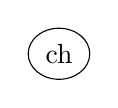
\begin{tikzpicture}[baseline=(n.base)]\node[draw,ellipse,inner sep=3pt] (n) {ch};\end{tikzpicture}}} and concrete \var{\over{c}{ch}}{\hand{ch}}{writing over}{ps_134-3_036-v0002}aracterization of test categories, \var{\xout{which}}{}{typewriter deletion}{ps_134-3_036-v0003} or possibly some
reinforcement still of that notion, which will imply stability under the
product operation.

Here it is tempting to use semi-simplicial techniques though, by lack
of independant foundations of homotopy theory in terms of the modelizer
(Cat). Thus we may want to take the map of semi-simplicial sets correspon-%
ding to (T) when passing to nerves, and express that a) this is a fibration
and b) the fibers of this fibration are "contractible"\var{\inserted[typed]{(or "aspheric")}}{(or "aspheric")}{typed insertion}{ps_134-3_036-v0004}, which together
will imply that we have a weak equivalence in (Ss sets). Or we may follow
the suggestion of Quillen's set-up, working heuristically in (Cat) as though
we actually knew it is a model category, and expressing that the adjunction
morphism in (T), which is a functor between categories, is actually a
"fibration", and that it\hand{'}s fibers are "contractible" namely weakly equivalent
to a one-point category. I\var{\over{n}{n}}{\hand{n}}{writing over}{ps_134-3_036-v0005} any case, a minimum amount of technique seems
needed here, to give the necessary clues for pursuing.

14.3.

30. Since Last week when I stopped with my notes, I got involved a bit
with recalling to mind the "Lego-Teichmüller construction game" for descri-%
bing in a conrete, "visual" way the Teichmüller groups of all possible
types and the main relationships between them, which I had first met with
last year. This and other non mathematical occupations left little time
only for my reflections on homotopy theory, \var{\inserted{which I took up}}{\hand{which I took up}}{insertion}{ps_134-3_036-v0006} mainly last night and today.
T\var{\over{h}{h}}{\hand{h}}{writing over}{ps_134-3_036-v0007}e focus of attention was the "technical point" of getting a handy carac-%
terization of test categories. The situation I feel is beginning to clari-%
fy somewhat. Last thing I did\hand{,} before reading last weeks' notes and getting
back to the typewriter\hand{,} was to get rid of a delusion which I was dragging
along more or less from the beginning of these notes, namely that our
basic modelizer (Cat), which we were using \var{\xout{for our}}{}{typewriter deletion}{ps_134-3_036-v0008} as \var{\over{p}{g}}{\hand{g}}{writing over}{ps_134-3_036-v0009}iving the most
natural definition of (Hot) in our setting, was a "model category" in the
sense of Quillen, more specifically a "closed model category", where
the "weak equivalences" are the homotopy equivalences of course, and where
cofibrations are just monomorphisms (namely functors injective on objects
and on arrows) - fibrations being defined in terms of these by the
\margin{\diagram{\begin{tikzpicture}[x=1em,y=1em]\draw (0,0)--(0,-3.6);\end{tikzpicture}}} Serre-Quillen lifting property. Without \var{\inserted[typed]{even}}{even}{typed insertion}{ps_134-3_036-v0010} being so demanding, it turns out
still that there is no reasonable structure of a model catégory on (Cat),
having the correct weak equivalences, and such that the standart \var{\inserted{"Kan}}{\hand{"Kan}}{insertion}{ps_134-3_036-v0011} inclusi-%
ons\hand{"} of the following two ordered sets

%% END SOURCE ps_134-3_036
\ifnum\EditionMode=1
\psapparatusstart
\psentry{ps_134-3_036-v0001}{1}{insertion}{\inserted{we started with}}{\hand{we started with}}{The handwritten insertion is incorporated at its indicated position; insertion brackets leave the running text.}
\psentry{ps_134-3_036-v0002}{2}{writing over}{\over{c}{ch}}{\hand{ch}}{The superposed handwritten reading replaces the underlying reading.}
\psentry{ps_134-3_036-v0003}{3}{typewriter deletion}{\xout{which}}{}{The typewriter strikes out this material; it leaves the corrected running text.}
\psentry{ps_134-3_036-v0004}{4}{typed insertion}{\inserted[typed]{(or "aspheric")}}{(or "aspheric")}{The typed insertion is incorporated at its indicated position; insertion brackets leave the running text.}
\psentry{ps_134-3_036-v0005}{5}{writing over}{\over{n}{n}}{\hand{n}}{The superposed handwritten reading replaces the underlying reading.}
\psentry{ps_134-3_036-v0006}{6}{insertion}{\inserted{which I took up}}{\hand{which I took up}}{The handwritten insertion is incorporated at its indicated position; insertion brackets leave the running text.}
\psentry{ps_134-3_036-v0007}{7}{writing over}{\over{h}{h}}{\hand{h}}{The superposed handwritten reading replaces the underlying reading.}
\psentry{ps_134-3_036-v0008}{8}{typewriter deletion}{\xout{for our}}{}{The typewriter strikes out this material; it leaves the corrected running text.}
\psentry{ps_134-3_036-v0009}{9}{writing over}{\over{p}{g}}{\hand{g}}{The superposed handwritten reading replaces the underlying reading.}
\psentry{ps_134-3_036-v0010}{10}{typed insertion}{\inserted[typed]{even}}{even}{The typed insertion is incorporated at its indicated position; insertion brackets leave the running text.}
\psentry{ps_134-3_036-v0011}{11}{insertion}{\inserted{"Kan}}{\hand{"Kan}}{The handwritten insertion is incorporated at its indicated position; insertion brackets leave the running text.}
\psapparatusend
\fi
\pssource{ps_134-3_037}{134-3/37}{https://grothendieck.umontpellier.fr/web/viewer.html?file=../134-3.pdf\#page=38}
\psnumber{ps_134-3_037-v0001}{1}
\psnumber{ps_134-3_037-v0002}{2}
\psnumber{ps_134-3_037-v0003}{3}
\psnumber{ps_134-3_037-v0004}{4}
\psnumber{ps_134-3_037-v0005}{5}
\psnumber{ps_134-3_037-v0006}{6}
\psnumber{ps_134-3_037-v0007}{7}
\psnumber{ps_134-3_037-v0008}{8}
\psnumber{ps_134-3_037-v0009}{9}
\psnumber{ps_134-3_037-v0010}{10}
\psnumber{ps_134-3_037-v0011}{11}
%% BEGIN SOURCE ps_134-3_037
% Pursuing Stacks (cotes 134-2 to 134-8): archive cote 134-3, site page 37 (PDF page 38), typescript page 37.
% typescript. Draft compared: ps2.tex:1781-1845.
% AI-transcribed by Claude Opus 5.5 (claude-opus-5-5, adaptive thinking, effort high), Message Batches API, batch ps1 (msgbatch_01Rv5hCaNTtUt4JHx1yqoHPL), 2026-11-12; image review recorded in records/CHECK_DECISIONS_134_3_4.tsv.
\scanpage{134-3/37}
\mspage{\hand{37}}
\hand{\diagram{\begin{tikzcd}[row sep=small,column sep=small] \& b \\ a \ar[ur]\ar[r] \& c \end{tikzcd}}} \quad and \quad \hand{\diagram{\begin{tikzcd}[row sep=small,column sep=small] a \ar[r] \& c \\ b \ar[ur] \& \end{tikzcd}}}
into
\[ \hand{\Delta}_2 = \hand{a\longrightarrow b\longrightarrow c} \]
be cofibering. Namely, for a category C, to say that it is``fibering''
(over the final category e) with respect to one or the other monomorphism,
means respectively that every arrow in $\underline{C}$ has a left respectively a right
inverse - the two together mean that $\underline{C}$ is a groupoid. But groupoids are
definitely \uline{not} sufficient for describing arbitrary homotopy types, they
give rise only to sums of K(\hand{$\pi$},1) spaces \var{\xout{\unsure{(}}}{}{typewriter deletion}{ps_134-3_037-v0001} - thus contradicting Quillen's
statement that homotopy types can be described by ``models'' which are both
fibering and cofibering\hand{!}

The feeling however remains that any elementary modelizer, namely one
defined (up to equivalence) by a test category, should be a \var{\inserted[typed]{closed}}{closed}{typed insertion}{ps_134-3_037-v0002} model catego\unsure{ry}
% NOTE: the end of this line is cut by the right edge of the scan
in Quillen's sense - \var{\over{If}{I}}{\hand{I}}{writing over}{ps_134-3_037-v0003} find it hard to believe that this should be a spe%
% NOTE: the end of this line (hyphen?) is cut by the right edge of the scan
cial feature just of semi-simplicial complexes !

While trying to understand test categories, the notion of \uline{asphericity}
for a morphism of topoi
\[ f\colon X \hand{\longrightarrow} Y \]
came in naturally - this is a natural \var{\xout{g\unsure{ene}}}{}{typewriter deletion}{ps_134-3_037-v0004} variant of the notion of
n-acyclicity (concerned with commutative cohomology) which has been deve-%
lopped in the context of étale topology of schemes in SGA 4. It can be
expressed by ``localizing\var{\xout{\illegible{1}}}{}{typewriter deletion}{ps_134-3_037-v0005} upon Y '' the Artin-Mazur condition that f be
a weak equivalence, by demanding that the same remain true for the induced
morphisms of topoi
\[ X\mathrm{x}_{Y}Y' \hand{\longrightarrow} Y' \]
for any ``localization morphism'' Y'\hand{$\longrightarrow$} Y. In terms of the categories of
sheaves \var{\xout{\illegible{1}}}{}{typewriter deletion}{ps_134-3_037-v0006} E, F on X,Y , Y' can be defined by an object (equally called
Y') of F, the category of sheaves on Y' being F$_{/Y'}$ , and the fiber-pro-%
duct X' can be defined likewise by an object \var{\deleted{\unsure{X'}}}{}{deletion}{ps_134-3_037-v0007} of E, namely \var{\inserted{by (X'=}}{\hand{by (X'=}}{insertion}{ps_134-3_037-v0008} f$^{*}$(Y'),
hence the corresponding category of sheaves is E$_{/f^{*}(Y')}$ . In case the
functor f$^{*}$ associated to f admits a left adjoint f$_{\hand{!}}$ (namely if it commutes
to arbitrary inverse limits, not only to finite one's), the category
E$_{/f^{*}(Y')}$ can be interpreted conveniently as \var{\xout{E$_{/Y'}$}}{}{typewriter deletion}{ps_134-3_037-v0009} E$_{f_{\hand{!}}/Y'}$ (or simply E$_{/Y'}$
if f$_{\hand{!}}$ is implicit), whose objects are pairs
\[ (U,\emptyset) \quad , \quad U \hand{\in} \mathrm{Ob}\ E \ , \ \emptyset : f_{\hand{!}}(U) \hand{\longrightarrow} Y' \quad , \]
with obvious ``maps'' between such objects. For the time being I am mainly
interested in the case of a morphism of topoi defined by a functor \var{\over{\unsure{(}}{b}}{\hand{b}}{writing over}{ps_134-3_037-v0010}etween
categories, which I will denote by the same symbol f :
\[ f\colon C' \hand{\longrightarrow} C \quad \text{defines f or } \hand{\hat{\ }}f : \hand{\hat{\ }}C\hand{'} \hand{\to} \hand{\hat{\ }}C\var{\xout{\unsure{'}}}{}{typewriter deletion}{ps_134-3_037-v0011} \quad . \]

%% END SOURCE ps_134-3_037
\ifnum\EditionMode=1
\psapparatusstart
\psentry{ps_134-3_037-v0001}{1}{typewriter deletion}{\xout{\unsure{(}}}{}{The typewriter strikes out this material; it leaves the corrected running text.}
\psentry{ps_134-3_037-v0002}{2}{typed insertion}{\inserted[typed]{closed}}{closed}{The typed insertion is incorporated at its indicated position; insertion brackets leave the running text.}
\psentry{ps_134-3_037-v0003}{3}{writing over}{\over{If}{I}}{\hand{I}}{The superposed handwritten reading replaces the underlying reading.}
\psentry{ps_134-3_037-v0004}{4}{typewriter deletion}{\xout{g\unsure{ene}}}{}{The typewriter strikes out this material; it leaves the corrected running text.}
\psentry{ps_134-3_037-v0005}{5}{typewriter deletion}{\xout{\illegible{1}}}{}{The typewriter strikes out this material; it leaves the corrected running text.}
\psentry{ps_134-3_037-v0006}{6}{typewriter deletion}{\xout{\illegible{1}}}{}{The typewriter strikes out this material; it leaves the corrected running text.}
\psentry{ps_134-3_037-v0007}{7}{deletion}{\deleted{\unsure{X'}}}{}{The author cancels this material by hand; it leaves the corrected running text.}
\psentry{ps_134-3_037-v0008}{8}{insertion}{\inserted{by (X'=}}{\hand{by (X'=}}{The handwritten insertion is incorporated at its indicated position; insertion brackets leave the running text.}
\psentry{ps_134-3_037-v0009}{9}{typewriter deletion}{\xout{E$_{/Y'}$}}{}{The typewriter strikes out this material; it leaves the corrected running text.}
\psentry{ps_134-3_037-v0010}{10}{writing over}{\over{\unsure{(}}{b}}{\hand{b}}{The superposed handwritten reading replaces the underlying reading.}
\psentry{ps_134-3_037-v0011}{11}{typewriter deletion}{$\xout{\unsure{'}}$}{}{The typewriter strikes out this material; it leaves the corrected running text.}
\psapparatusend
\fi
\pssource{ps_134-3_038}{134-3/38}{https://grothendieck.umontpellier.fr/web/viewer.html?file=../134-3.pdf\#page=39}
\psnumber{ps_134-3_038-v0001}{1}
\psnumber{ps_134-3_038-v0002}{2}
\psnumber{ps_134-3_038-v0003}{3}
\psnumber{ps_134-3_038-v0004}{4}
\psnumber{ps_134-3_038-v0005}{5}
\psnumber{ps_134-3_038-v0006}{6}
\psnumber{ps_134-3_038-v0007}{7}
\psnumber{ps_134-3_038-v0008}{8}
\psnumber{ps_134-3_038-v0009}{9}
\psnumber{ps_134-3_038-v0010}{10}
\psnumber{ps_134-3_038-v0011}{11}
\psnumber{ps_134-3_038-v0012}{12}
\psnumber{ps_134-3_038-v0013}{13}
\psnumber{ps_134-3_038-v0014}{14}
\psnumber{ps_134-3_038-v0015}{15}
\psnumber{ps_134-3_038-v0016}{16}
\psnumber{ps_134-3_038-v0017}{17}
\psnumber{ps_134-3_038-v0018}{18}
\psnumber{ps_134-3_038-v0019}{19}
\psnumber{ps_134-3_038-v0020}{20}
\psnumber{ps_134-3_038-v0021}{21}
%% BEGIN SOURCE ps_134-3_038
% Pursuing Stacks (cotes 134-2 to 134-8): archive cote 134-3, site page 38 (PDF page 39), typescript page 38.
% typescript. Draft compared: ps2.tex:1831-1909.
% AI-transcribed by Claude Opus 5.5 (claude-opus-5-5, adaptive thinking, effort high), Message Batches API, batch ps1 (msgbatch_01Rv5hCaNTtUt4JHx1yqoHPL), 2026-11-12; image review recorded in records/CHECK_DECISIONS_134_3_4.tsv.
\scanpage{134-3/38}
\mspage{\hand{38}}
Using the fact that in the \var{\xout{description of}}{}{typewriter deletion}{ps_134-3_038-v0001} general definition of asphericity
it is enough to take Y' in a family of generators of the topos Y,  and \var{\xout{usin}}{}{typewriter deletion}{ps_134-3_038-v0002}
using here the generating subcategory C of $\overset{\hand{\wedge}}{C}$ ,  we get the following crite\var{\xout{r}}{}{typewriter deletion}{ps_134-3_038-v0003}
\unsure{t}ion for asphericity of $\overset{\hand{\wedge}}{f}$ :  if is nec. and sufficient that for every
\hand{$a\in$}Ob C ,  the induced morphism of topoi
\[ \overset{\hand{\wedge}}{C'}_{/a} \hand{\cong} (C'_{/a})^{\hand{\wedge}} \hand{\to} \overset{\hand{\wedge}}{C}_{/a} \hand{\simeq} (C_{/a})^{\hand{\wedge}} \]
be a weak equivalence,  i.e. that the natural functor  $C'_{/a}\hand{\to} C_{/a}$ be a weak
equivalence.  But it is immediate that $C_{/a}$ is ``contractible'' \var{\xout{i.e.}}{}{typewriter deletion}{ps_134-3_038-v0004} \hand{i.e.} ``asphe
ric'',  namely the ``map'' from $C_{/a}$ to the final category is a weak equivalen\var{\xout{c}}{}{typewriter deletion}{ps_134-3_038-v0005}
ce (this is true for any category having a final object). Therefore we get
the following
\margin{\diagram{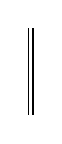
\begin{tikzpicture}\draw (0,0)--(0,1.1);\draw (.06,0)--(.06,1.1);\end{tikzpicture}}}\uline{Criterion of asphericity for a functor} f: C'$\hand{\to}$ C  between categories:
namely it is n. and s. that for any a $\hand{\in}$ Ob C,   $C'_{/a}$  be aspheric.

Let's come back to a \var{\xout{would}}{}{typewriter deletion}{ps_134-3_038-v0006} category A,  for which we want to express
that it is a test-category,  namely for any \var{\inserted{[small]}}{\hand{[small]}}{insertion}{ps_134-3_038-v0007} category B,  the natural
functor
\[ \hand{(*)} \qquad i_Aj_A(B) \hand{\longrightarrow} B \]
is a weak equivalence.  O\var{\over{n}{n}}{\hand{n}}{writing over}{ps_134-3_038-v0008}e immediately checks that for any b$\hand{\in}$ Ob B,
the category  $i_Aj_A(B)_{/b}$ \var{\xout{over}}{}{typewriter deletion}{ps_134-3_038-v0009} over $B_{/b}$  is isomorphic to $i_Aj_A(B_{/b})$ . Hence
we get the following
\uline{Proposition}  For a \var{\inserted{[small]}}{\hand{[small]}}{insertion}{ps_134-3_038-v0010} category A,  the following are equivalent:
(i)  A is a test category,  namely (*) is a\var{\deleted{n}}{}{deletion}{ps_134-3_038-v0011} \var{\inserted{weak}}{\hand{weak}}{insertion}{ps_134-3_038-v0012} equivalence for any \var{\inserted{[small]}}{\hand{[small]}}{insertion}{ps_134-3_038-v0013}
category B.
(ii)  (*) is aspheric for any \var{\inserted{[small]}}{\hand{[small]}}{insertion}{ps_134-3_038-v0014} category B.
(iii)  $i_Aj_A(B)$ is aspheric for any category B with final element.

This latter condition,  which is the most ``concrete'' one so far,
means also that the element
\[ F = j_A(B) = (\ a \hand{\mapsto} \mathrm{Hom}(\underset{\hand{\wedge}}{A}_{/a},B)) \hand{\in} \overset{\hand{\wedge}}{A} \]
is \var{\deleted{an}}{}{deletion}{ps_134-3_038-v0015} \var{\inserted[typed]{aspheric}}{aspheric}{typed insertion}{ps_134-3_038-v0016} \var{\deleted{\xout{aspheric}}}{}{deletion}{ps_134-3_038-v0017} element of the topos $\overset{\hand{\wedge}}{A}$ ,  namely  the induced topos $\overset{\hand{\wedge}}{A}_{/F}$ is
aspheric (i.e. the category $A_{/F}$  is aspheric),  \uline{whenever} B has a final
element.

\hand{31.}  For the notion of a test category to make at all a sense,  we should
make sure in the long last that \hand{$\Delta$} itself,  the category of standar\var{\over{t}{d}}{\hand{d}}{writing over}{ps_134-3_038-v0018} simpli-%
ces,  is indeed a test category.  So I finally set out to prove at least
\margin{$\times$} that much,  using the few reflexes I ha\var{\over{d}{v}}{\hand{v}}{writing over}{ps_134-3_038-v0019}e in semi-simplicial homotopy theo\var{\xout{r}}{}{typewriter deletion}{ps_134-3_038-v0020}-%
ry.  A proof finally peeled out it seems,  giving clues for handy conditi-%
ons in the general case,  which should be \uline{sufficient} \var{\over{\unsure{in the base}}{at least}}{\hand{at least}}{writing over}{ps_134-3_038-v0021} to insure
that B is a test category,  but maybe not quite necessary.  I'll try now
to get it down explicitly.

%% END SOURCE ps_134-3_038
\ifnum\EditionMode=1
\psapparatusstart
\psentry{ps_134-3_038-v0001}{1}{typewriter deletion}{\xout{description of}}{}{The typewriter strikes out this material; it leaves the corrected running text.}
\psentry{ps_134-3_038-v0002}{2}{typewriter deletion}{\xout{usin}}{}{The typewriter strikes out this material; it leaves the corrected running text.}
\psentry{ps_134-3_038-v0003}{3}{typewriter deletion}{\xout{r}}{}{The typewriter strikes out this material; it leaves the corrected running text.}
\psentry{ps_134-3_038-v0004}{4}{typewriter deletion}{\xout{i.e.}}{}{The typewriter strikes out this material; it leaves the corrected running text.}
\psentry{ps_134-3_038-v0005}{5}{typewriter deletion}{\xout{c}}{}{The typewriter strikes out this material; it leaves the corrected running text.}
\psentry{ps_134-3_038-v0006}{6}{typewriter deletion}{\xout{would}}{}{The typewriter strikes out this material; it leaves the corrected running text.}
\psentry{ps_134-3_038-v0007}{7}{insertion}{\inserted{[small]}}{\hand{[small]}}{The handwritten insertion is incorporated at its indicated position; insertion brackets leave the running text.}
\psentry{ps_134-3_038-v0008}{8}{writing over}{\over{n}{n}}{\hand{n}}{The superposed handwritten reading replaces the underlying reading.}
\psentry{ps_134-3_038-v0009}{9}{typewriter deletion}{\xout{over}}{}{The typewriter strikes out this material; it leaves the corrected running text.}
\psentry{ps_134-3_038-v0010}{10}{insertion}{\inserted{[small]}}{\hand{[small]}}{The handwritten insertion is incorporated at its indicated position; insertion brackets leave the running text.}
\psentry{ps_134-3_038-v0011}{11}{deletion}{\deleted{n}}{}{The author cancels this material by hand; it leaves the corrected running text.}
\psentry{ps_134-3_038-v0012}{12}{insertion}{\inserted{weak}}{\hand{weak}}{The handwritten insertion is incorporated at its indicated position; insertion brackets leave the running text.}
\psentry{ps_134-3_038-v0013}{13}{insertion}{\inserted{[small]}}{\hand{[small]}}{The handwritten insertion is incorporated at its indicated position; insertion brackets leave the running text.}
\psentry{ps_134-3_038-v0014}{14}{insertion}{\inserted{[small]}}{\hand{[small]}}{The handwritten insertion is incorporated at its indicated position; insertion brackets leave the running text.}
\psentry{ps_134-3_038-v0015}{15}{deletion}{\deleted{an}}{}{The author cancels this material by hand; it leaves the corrected running text.}
\psentry{ps_134-3_038-v0016}{16}{typed insertion}{\inserted[typed]{aspheric}}{aspheric}{The typed insertion is incorporated at its indicated position; insertion brackets leave the running text.}
\psentry{ps_134-3_038-v0017}{17}{deletion}{\deleted{\xout{aspheric}}}{}{The author cancels this material by hand; it leaves the corrected running text.}
\psentry{ps_134-3_038-v0018}{18}{writing over}{\over{t}{d}}{\hand{d}}{The superposed handwritten reading replaces the underlying reading.}
\psentry{ps_134-3_038-v0019}{19}{writing over}{\over{d}{v}}{\hand{v}}{The superposed handwritten reading replaces the underlying reading.}
\psentry{ps_134-3_038-v0020}{20}{typewriter deletion}{\xout{r}}{}{The typewriter strikes out this material; it leaves the corrected running text.}
\psentry{ps_134-3_038-v0021}{21}{writing over}{\over{\unsure{in the base}}{at least}}{\hand{at least}}{The superposed handwritten reading replaces the underlying reading.}
\psapparatusend
\fi
\pssource{ps_134-3_039}{134-3/39}{https://grothendieck.umontpellier.fr/web/viewer.html?file=../134-3.pdf\#page=40}
\psnumber{ps_134-3_039-v0001}{1}
\psnumber{ps_134-3_039-v0002}{2}
\psnumber{ps_134-3_039-v0003}{3}
\psnumber{ps_134-3_039-v0004}{4}
\psnumber{ps_134-3_039-v0005}{5}
\psnumber{ps_134-3_039-v0006}{6}
\psnumber{ps_134-3_039-v0007}{7}
\psnumber{ps_134-3_039-v0008}{8}
\psnumber{ps_134-3_039-v0009}{9}
\psnumber{ps_134-3_039-v0010}{10}
\psnumber{ps_134-3_039-v0011}{11}
\psnumber{ps_134-3_039-v0012}{12}
%% BEGIN SOURCE ps_134-3_039
% Pursuing Stacks (cotes 134-2 to 134-8): archive cote 134-3, site page 39 (PDF page 40), typescript page 39.
% typescript. Draft compared: ps2.tex:1894-1966.
% AI-transcribed by Claude Opus 5.5 (claude-opus-5-5, adaptive thinking, effort high), Message Batches API, batch ps1 (msgbatch_01Rv5hCaNTtUt4JHx1yqoHPL), 2026-11-12; image review recorded in records/CHECK_DECISIONS_134_3_4.tsv.
\scanpage{134-3/39}
\margin{cf théorème p 46}
\mspage{\hand{39}} \margin{\unsure{K}}

Here are the conditions I got:
(T 1) A is aspheric .
(T 2\var{\over{)}{)}}{\hand{)}}{writing over}{ps_134-3_039-v0001} For $a,b \hand{\in}$ Ob A, $A_{/axb}$ is aspheric \var{\inserted{i.e. for any $a \in \mathrm{Ob}\, A$, $A_{/a} \to A$ is aspheric}}{\hand{i.e. for any $a \in \mathrm{Ob}\, A$, $A_{/a} \to A$ is aspheric}}{insertion}{ps_134-3_039-v0002} (NB axb need not exist in A
but it is in any case well defined as an element of $\overset{\hand{\wedge}}{A}$ ).
(T 3) There exists an \uline{aspheric} element I of $\overset{\hand{\wedge}}{A}$ , and two subobjects
\margin{NB In view of \unsure{T1 et T2}, I aspheric $\Leftrightarrow$ $I \to e$ is aspheric}
$e_o$ and $e_1$ of I which are final elements of $\overset{\hand{\wedge}}{A}$ , such that
$e_o \hand{\cap} e_1$ $(\overset{def}{=} e_o \hand{\times}_I e_1) = \emptyset_{A^{\hand{\wedge}}}$ , the initial or ``empty'' element of $A\hand{\hat{}}$ .

In case when A = $\hand{\Delta}$ (as we\hand{l}l as in the cubical analogon $\hand{\Box}$ ), I took
I = $\hand{\Delta}_1$ which is an element of A itself, and \var{\deleted{the}}{}{deletion}{ps_134-3_039-v0003} moreover A has a final
element (which is a final element of $A^{\hand{\wedge}}$\hand{/}therefore) e , thus $e_o$ and $e_1$ are
defined by well defined arrows in A itself, namely $\hand{\delta}_o$ and $\hand{\delta}_1$ . But it
does not seem that these special features are really relevant. In any case
\uline{intuitively I stands for the unit interval}, \uline{with endpoints} $e_o$ , $e_1$ . If
F is any element in $A^{\hand{\wedge}}$, the standard way for trying to prove it is asphe-%
ric would be to prove that we can find a ``constant map'' F $\hand{\to}$ F, namely one
\var{\inserted[typed]{which}}{which}{typed insertion}{ps_134-3_039-v0004} factors into
\margin{\unsure{$\mathcal{A}$}}
\[ F \hand{\longrightarrow} e \overset{c}{\hand{\longrightarrow}} F \qquad \text{(e the final element of \var{\deleted{\illegible{1}}}{}{deletion}{ps_134-3_039-v0005} \hand{$A^{\hand{\wedge}} = \overset{\hand{\wedge}}{A}$)}} \]
for suitable \hand{c} : e $\hand{\to}$ F or ``section'' of F, which be ``homotopic'' to the
identity map F$\hand{\to}$F. When trying to make explicit the notion of a ``homotopy''
\var{\inserted[typed]{h}}{h}{typed insertion}{ps_134-3_039-v0006} between two such maps, more generally between two \var{\inserted{$f_o, f_1$ :}}{\hand{$f_o, f_1$ :}}{insertion}{ps_134-3_039-v0007} maps F $\hand{\rightrightarrows}$ G , we
hit of course upon the arrow h in the following diagram, which should
make it commutative

\hand{(D)}
\diagram{
% Hand-drawn arrows are marked blue; typed objects remain plain.
\begin{tikzcd}
 \& F \mathrm{x} I \ar[dd, dashed, color=blue, "\hand{h}"'] \& \\
F \hand{\simeq} F \mathrm{x} e_o \ar[ur, hook, color=blue] \ar[dr, color=blue, "f_o"'] \& \& F \hand{\simeq} F \mathrm{x} e_1 \ar[ul, hook, color=blue] \ar[dl, color=blue, "f_1"] \\
 \& G \&
\end{tikzcd}
}
.

This notion of a homotopy is defined in any category \var{\inserted{$\mathcal{A}$}}{\hand{$\mathcal{A}$}}{insertion}{ps_134-3_039-v0008} where we got an
element I and two subobjects $e_o$ , $e_1$ which are final objects. Suppose we
\var{\inserted[typed]{got such h, and we}}{got such h, and we}{typed insertion}{ps_134-3_039-v0009} know moreover \var{\xout{that}}{}{typewriter deletion}{ps_134-3_039-v0010} (for given F,G,$f_o$,$f_1$,h) that the two inclusions of
$Fxe_o$ and $Fxe_1$ into FxI are weak equivalences, and that $f_o$ is a weak equi-%
valence (for a given set of arrows called ``weak equivalences'', for instan-%
ce defined in terms of a``topology'' on \hand{$\mathcal{A}$} , in the present case the canoni-%
cal topology of the topos $A\hand{\hat{}}$ ) ; then it follows (with the usual ``mild
saturation\var{\unsure{\xout{''}}}{}{typewriter deletion}{ps_134-3_039-v0011} condition'' on the notion of weak equivalence) that h, and hence
$f_1$ are weak equivalences. Coming back to the case F=G, $f_o$ = $id_F$ , $f_1$ =
``constant map'' defined by a c: e $\hand{\to}$ F , we get that this constant map
$f_1$ is a weak equivalence. Does this imply that F $\hand{\to}$ e is equally a weak
equivalence ? This is not quite formal for general (\hand{$\mathcal{A}$}, W), but it is \var{\xout{so}}{}{typewriter deletion}{ps_134-3_039-v0012}
true though in the case \hand{$\mathcal{A}$} = $A^{\hand{\wedge}}$ and with the usual meaning of ``weak equiva-%

%% END SOURCE ps_134-3_039
\ifnum\EditionMode=1
\psapparatusstart
\psentry{ps_134-3_039-v0001}{1}{writing over}{\over{)}{)}}{\hand{)}}{The superposed handwritten reading replaces the underlying reading.}
\psentry{ps_134-3_039-v0002}{2}{insertion}{\inserted{i.e. for any $a \in \mathrm{Ob}\, A$, $A_{/a} \to A$ is aspheric}}{\hand{i.e. for any $a \in \mathrm{Ob}\, A$, $A_{/a} \to A$ is aspheric}}{The handwritten insertion is incorporated at its indicated position; insertion brackets leave the running text.}
\psentry{ps_134-3_039-v0003}{3}{deletion}{\deleted{the}}{}{The author cancels this material by hand; it leaves the corrected running text.}
\psentry{ps_134-3_039-v0004}{4}{typed insertion}{\inserted[typed]{which}}{which}{The typed insertion is incorporated at its indicated position; insertion brackets leave the running text.}
\psentry{ps_134-3_039-v0005}{5}{deletion}{\deleted{\illegible{1}}}{}{The author cancels this material by hand; it leaves the corrected running text.}
\psentry{ps_134-3_039-v0006}{6}{typed insertion}{\inserted[typed]{h}}{h}{The typed insertion is incorporated at its indicated position; insertion brackets leave the running text.}
\psentry{ps_134-3_039-v0007}{7}{insertion}{\inserted{$f_o, f_1$ :}}{\hand{$f_o, f_1$ :}}{The handwritten insertion is incorporated at its indicated position; insertion brackets leave the running text.}
\psentry{ps_134-3_039-v0008}{8}{insertion}{\inserted{$\mathcal{A}$}}{\hand{$\mathcal{A}$}}{The handwritten insertion is incorporated at its indicated position; insertion brackets leave the running text.}
\psentry{ps_134-3_039-v0009}{9}{typed insertion}{\inserted[typed]{got such h, and we}}{got such h, and we}{The typed insertion is incorporated at its indicated position; insertion brackets leave the running text.}
\psentry{ps_134-3_039-v0010}{10}{typewriter deletion}{\xout{that}}{}{The typewriter strikes out this material; it leaves the corrected running text.}
\psentry{ps_134-3_039-v0011}{11}{typewriter deletion}{\unsure{\xout{''}}}{}{All material inside this wrapper is cancelled. Its original doubt and presentation remain in the diplomatic text and apparatus; no empty doubt mark or page label is inserted into the corrected running text.}
\psentry{ps_134-3_039-v0012}{12}{typewriter deletion}{\xout{so}}{}{The typewriter strikes out this material; it leaves the corrected running text.}
\psapparatusend
\fi
\pssource{ps_134-3_040}{134-3/40}{https://grothendieck.umontpellier.fr/web/viewer.html?file=../134-3.pdf\#page=41}
\psnumber{ps_134-3_040-v0001}{1}
\psnumber{ps_134-3_040-v0002}{2}
\psnumber{ps_134-3_040-v0003}{3}
\psnumber{ps_134-3_040-v0004}{4}
\psnumber{ps_134-3_040-v0005}{5}
\psnumber{ps_134-3_040-v0006}{6}
\psnumber{ps_134-3_040-v0007}{7}
\psnumber{ps_134-3_040-v0008}{8}
\psnumber{ps_134-3_040-v0009}{9}
\psnumber{ps_134-3_040-v0010}{10}
\psnumber{ps_134-3_040-v0011}{11}
\psnumber{ps_134-3_040-v0012}{12}
\psnumber{ps_134-3_040-v0013}{13}
\psnumber{ps_134-3_040-v0014}{14}
%% BEGIN SOURCE ps_134-3_040
% Pursuing Stacks (cotes 134-2 to 134-8): archive cote 134-3, site page 40 (PDF page 41), typescript page 40.
% typescript. Draft compared: ps2.tex:1954-2026.
% AI-transcribed by Claude Opus 5.5 (claude-opus-5-5, adaptive thinking, effort high), Message Batches API, batch ps1 (msgbatch_01Rv5hCaNTtUt4JHx1yqoHPL), 2026-11-12; image review recorded in records/CHECK_DECISIONS_134_3_4.tsv.
\scanpage{134-3/40}
\mspage{\hand{4\unsure{0}.}}

lence",  in this case it is true indeed that if we have a situation of
inclusion with re\var{\xout{x}}{}{typewriter deletion}{ps_134-3_040-v0001}traction  $E\hand{\to} F$ and $F\hand{\to} E$  ($E$ need not be a final ele-%
ment of \hand{$\mathcal{A}$} ),  such that the comp\var{\xout{p}}{}{typewriter deletion}{ps_134-3_040-v0002}ositum  $p$: $F\hand{\to} E\hand{\to} F$  (a projector in
$F$) is a weak equivalence,  then so are $E\hand{\to} F$ and $F\hand{\to} E$.  To check this,
we are reduced to check the corresponding statement in (Cat),  in fact we
can check it in the more general situation with two topoi $E$ and $F$,  using
the Artin-Mazur criterion.  (We get first that $E\hand{\to} F$ is a weak equivalence,
and hence by saturation that $F\hand{\to} E$ is too.)

Thus the assumptions\hand{/}made on $F\hand{\in} \mathrm{Ob}\,A^{\hand{\wedge}}$ impl\var{\over{ies}{y}}{\hand{y}}{writing over}{ps_134-3_040-v0003} that  $F\hand{\to} e$ is a weak
equivalence i.e.  $A_{/F}\hand{\to} A$ is a weak equivalence,  and if we assume now
that $A$ satisfies (T 1) namely $A$ is aspheric,  so is $F$.

We apply this to the case  $F = j_A(B) = (\ a\hand{\mapsto} \mathrm{Hom}(A_{/a},B))$,  where $B$
is a \var{\inserted{[small]}}{\hand{[small]}}{insertion}{ps_134-3_040-v0004} category with final element.  We have to check (using T 1 to T 3):

a) the inclusions \var{\inserted[typed]{of}}{of}{typed insertion}{ps_134-3_040-v0005} $F\mathrm{x}e_o$ , $F\mathrm{x}e_1$ into $F$\hand{x}$I$ are weak equivalences (this will
be true in\hand{/}fact for any $F\hand{\in}\mathrm{Ob}\,A$\hand{$\hat{}$}),

b) there exists a "homotopy" h making commutative the previous diagram \var{\inserted{(D)}}{\hand{(D)}}{insertion}{ps_134-3_040-v0006},
where \var{\inserted{$G=F$, $f_0=\mathrm{id}_F$, and}}{\hand{$G=F$, $f_0=\mathrm{id}_F$, and}}{insertion}{ps_134-3_040-v0007} $f_1$:  $F\hand{\to} F$ is the "constant map" defined by the section
$c : e\hand{\to} F$ of $F$,  associating to every $a\hand{\in} A$ the \uline{constant} functor
$e_{a,B}$: $A_{/a}\hand{\to} B$  with value $e_B$ (a fixed final element of $B$),  thus
$e_{a,B}\hand{\in} F(a) = \mathrm{Hom}(A_{/a},B)$  (and it is clear that this is "functorial
in a").

Then  a) and b) will imply that $F$ is aspheric - hence $A$ is a test-category
by the criterion (iii) of the proposition above.

To check b) we do not make use of \var{\inserted{(T1) nor}}{\hand{(T1) nor}}{insertion}{ps_134-3_040-v0008} (T 2),  nor of the asphericity of
$I$.  We have to define a "map"
\[ h\colon F\mathrm{x}I\hand{\to} F\ , \]
i.e. for every $a\hand{\in}\mathrm{Ob}\,A$,  a map (functorial for variable a)
\[ h(a)\colon\ \mathrm{Hom}(A_{/a},\ B)\ \mathrm{x}\ \mathrm{Hom}(a,I)\hand{\longrightarrow} \mathrm{Hom}(A_{/a},B) \]
(two of the Hom's are in (Cat), the other is in $A^{\hand{\wedge}}$).  Thus,  let
\[ f\colon A_{/a}\hand{\to} B\ ,\quad u\colon a\hand{\longrightarrow} I\ \ , \]
we must define
\[ \var{\over{h(a)}{h(a)}}{\hand{h(a)}}{writing over}{ps_134-3_040-v0009}(f,u)\ :\ A_{/a}\hand{\to} B\ ,\ \var{\xout{(a functor from A_{/a} to B)}}{}{typewriter deletion}{ps_134-3_040-v0010} \]
a functor from $A_{/a}$ to $B$,  depending on the choice of $f$ and $u$.  Now let ,
for any  $u\hand{\in}\mathrm{Hom}(a,I)$, \var{\xout{x}}{}{typewriter deletion}{ps_134-3_040-v0011} $u$: $a\hand{\to} I$,  $a_u$ be defined in $A^{\hand{\wedge}}$\hand{/}as
\[ a_u = u^{-1}(e_o) = (a,u)\mathrm{x}_I e_o\qquad , \]
viewed as a subobject of a,  and hence \var{\inserted{$C_u=$}}{\hand{$C_u=$}}{insertion}{ps_134-3_040-v0012}$A_{/a_u}$  can be viewed as a subcategory
of \var{\inserted{$C=$}}{\hand{$C=$}}{insertion}{ps_134-3_040-v0013}$A_{/a}$ ,  namely the  full subcategory of those \var{\xout{arrx}}{}{typewriter deletion}{ps_134-3_040-v0014} objects \hand{$x$} over a
i.e. arrows \hand{$x$}$\hand{\to} a$ in $A$,  which factor through $a_u$ namely such that the
compositum  \hand{$x$}$\hand{\to} a\hand{\to} I$  factors through $e_o$ .  This subcategory is clearly

%% END SOURCE ps_134-3_040
\ifnum\EditionMode=1
\psapparatusstart
\psentry{ps_134-3_040-v0001}{1}{typewriter deletion}{\xout{x}}{}{The typewriter strikes out this material; it leaves the corrected running text.}
\psentry{ps_134-3_040-v0002}{2}{typewriter deletion}{\xout{p}}{}{The typewriter strikes out this material; it leaves the corrected running text.}
\psentry{ps_134-3_040-v0003}{3}{writing over}{\over{ies}{y}}{\hand{y}}{The superposed handwritten reading replaces the underlying reading.}
\psentry{ps_134-3_040-v0004}{4}{insertion}{\inserted{[small]}}{\hand{[small]}}{The handwritten insertion is incorporated at its indicated position; insertion brackets leave the running text.}
\psentry{ps_134-3_040-v0005}{5}{typed insertion}{\inserted[typed]{of}}{of}{The typed insertion is incorporated at its indicated position; insertion brackets leave the running text.}
\psentry{ps_134-3_040-v0006}{6}{insertion}{\inserted{(D)}}{\hand{(D)}}{The handwritten insertion is incorporated at its indicated position; insertion brackets leave the running text.}
\psentry{ps_134-3_040-v0007}{7}{insertion}{\inserted{$G=F$, $f_0=\mathrm{id}_F$, and}}{\hand{$G=F$, $f_0=\mathrm{id}_F$, and}}{The handwritten insertion is incorporated at its indicated position; insertion brackets leave the running text.}
\psentry{ps_134-3_040-v0008}{8}{insertion}{\inserted{(T1) nor}}{\hand{(T1) nor}}{The handwritten insertion is incorporated at its indicated position; insertion brackets leave the running text.}
\psentry{ps_134-3_040-v0009}{9}{writing over}{$\over{h(a)}{h(a)}$}{$\hand{h(a)}$}{The superposed handwritten reading replaces the underlying reading.}
\psentry{ps_134-3_040-v0010}{10}{typewriter deletion}{$\xout{(a functor from A_{/a} to B)}$}{}{The typewriter strikes out this material; it leaves the corrected running text.}
\psentry{ps_134-3_040-v0011}{11}{typewriter deletion}{\xout{x}}{}{The typewriter strikes out this material; it leaves the corrected running text.}
\psentry{ps_134-3_040-v0012}{12}{insertion}{\inserted{$C_u=$}}{\hand{$C_u=$}}{The handwritten insertion is incorporated at its indicated position; insertion brackets leave the running text.}
\psentry{ps_134-3_040-v0013}{13}{insertion}{\inserted{$C=$}}{\hand{$C=$}}{The handwritten insertion is incorporated at its indicated position; insertion brackets leave the running text.}
\psentry{ps_134-3_040-v0014}{14}{typewriter deletion}{\xout{arrx}}{}{The typewriter strikes out this material; it leaves the corrected running text.}
\psapparatusend
\fi
\pssource{ps_134-3_041}{134-3/41}{https://grothendieck.umontpellier.fr/web/viewer.html?file=../134-3.pdf\#page=42}
\psnumber{ps_134-3_041-v0001}{1}
\psnumber{ps_134-3_041-v0002}{2}
\psnumber{ps_134-3_041-v0003}{3}
\psnumber{ps_134-3_041-v0004}{4}
\psnumber{ps_134-3_041-v0005}{5}
\psnumber{ps_134-3_041-v0006}{6}
\psnumber{ps_134-3_041-v0007}{7}
\psnumber{ps_134-3_041-v0008}{8}
\psnumber{ps_134-3_041-v0009}{9}
\psnumber{ps_134-3_041-v0010}{10}
\psnumber{ps_134-3_041-v0011}{11}
\psnumber{ps_134-3_041-v0012}{12}
\psnumber{ps_134-3_041-v0013}{13}
\psnumber{ps_134-3_041-v0014}{14}
\psnumber{ps_134-3_041-v0015}{15}
\psnumber{ps_134-3_041-v0016}{16}
\psnumber{ps_134-3_041-v0017}{17}
\psnumber{ps_134-3_041-v0018}{18}
\psnumber{ps_134-3_041-v0019}{19}
\psnumber{ps_134-3_041-v0020}{20}
\psnumber{ps_134-3_041-v0021}{21}
\psnumber{ps_134-3_041-v0022}{22}
%% BEGIN SOURCE ps_134-3_041
% Pursuing Stacks (cotes 134-2 to 134-8): archive cote 134-3, site page 41 (PDF page 42), typescript page 41.
% typescript. Draft compared: ps2.tex:2009-2075.
% AI-transcribed by Claude Opus 5.5 (claude-opus-5-5, adaptive thinking, effort high), Message Batches API, batch ps1 (msgbatch_01Rv5hCaNTtUt4JHx1yqoHPL), 2026-11-12; image review recorded in records/CHECK_DECISIONS_134_3_4.tsv.
\scanpage{134-3/41}
\mspage{\hand{41}}

a "crible"\var{\inserted{[or ``sieve'']}}{\hand{[or ``sieve'']}}{insertion}{ps_134-3_041-v0001} in $A_{/a}$ , namely for an arrow $y\hand{\to} x$ in $A_{/a}$ , if the target x is
in the subcategory, so is the source y. This being so, we define \var{\over{a}{t}}{\hand{t}}{writing over}{ps_134-3_041-v0002}he
functor
\[ f' = h(f,u) \ : \ A_{/a}=C \hand{\to} B \]
by the conditions that
\[ f'\hand{\big|}(A_{/a_u} = C_u) \ = f\hand{\big|}C_u \]
\[ f'\hand{\big|}(C\hand{\setminus} C_u) \ = \text{constant functor with value } e_B\hand{\unsure{;}} \]
(where $C\hand{\setminus} C_u$ denotes the obvious \uline{full} subcategory of C , complementary to
$C_u$ )\hand{.} \var{\over{t}{T}}{\hand{T}}{writing over}{ps_134-3_041-v0003}his defines f' uniquely, \var{\xout{the}}{}{typewriter deletion}{ps_134-3_041-v0004} on the objects first, and on the
arrows too because the only arrows left \var{\xout{where}}{}{typewriter deletion}{ps_134-3_041-v0005} in C where we got still to
define f' are arrows $x \hand{\to} y$ with x \var{\over{\unsure{o}}{i}}{\hand{i}}{writing over}{ps_134-3_041-v0006}n $C_u$ and y in $C\hand{\setminus} C_u$ (because $C_u$ is a
crible), but then $f'(y) = e_B$ and we have no choice for $f'(x)\hand{\to} f'(y)$\hand{!}
It\hand{'}s trivial checking that this way we get indeed a \uline{functor}\var{\inserted{$f'$:}}{\hand{$f'$:}}{insertion}{ps_134-3_041-v0007} $C\hand{\to} B$, thus
the map h(a) is defined - and that this map is functorial with respect to
a, i.e. comes from a map h: $F\mathrm{x} I \hand{\to} F$ as we wanted. T\var{\over{\unsure{n}}{h}}{\hand{h}}{writing over}{ps_134-3_041-v0008}e commutativity
of (D) is easily checked\var{\over{\unsure{,}}{:}}{\hand{:}}{writing over}{ps_134-3_041-v0009} for the left triangle i.e. that the compositum
$F \hand{\simeq} F\mathrm{x} e_o \hand{\to} F\mathrm{x} I \overset{h}{\hand{\longrightarrow}} F$ is the identity, it comes from the fact that if u
factors through $e_o$ then $C_u = C$ hence $f' = f$ ; for the right triangle, it
comes from the fact that if u factors through $e_l$ th\var{\over{a}{e}}{\hand{e}}{writing over}{ps_134-3_041-v0010}n $C_u = \emptyset$ (here we use
the assumption $e_o\hand{\cap}e_l = \emptyset_{A\hand{^\wedge}}$), and hence f' is the constant functor $C\hand{\to} B$
with value $e_B$ . This settles b).

We have still to check a), namely that for any $F\hand{\in} \mathrm{Ob}\, A^{\hand{\wedge}}$, the inclusi-%
on\var{\deleted{s}}{}{deletion}{ps_134-3_041-v0011} of \var{\inserted{the objects}}{\hand{the objects}}{insertion}{ps_134-3_041-v0012} $F\mathrm{x} e_i$\hand{\unsure{,}} into $F\mathrm{x} I$ are weak equivalences, or what amounts to the same,
that the projection
\[ F\mathrm{x} I \hand{\longrightarrow} F \]
is a weak equivalence - this will be true in fact for any object I of $A^{\hand{\wedge}}$
which is aspheric. I\var{\over{n}{n}}{\hand{n}}{writing over}{ps_134-3_041-v0013}deed, we will prove the stronger result that
$F\mathrm{x} I \hand{\to} F$ is \uline{aspheric}, i.e. that the functor
\[ A_{/F\mathrm{x} I} \hand{\to} A_{/F} \]
is aspheric\hand{\unsure{.}} \var{\over{w}{W}}{\hand{W}}{writing over}{ps_134-3_041-v0014}e use for this the criterion of p. 38 , which here transla-%
tes into the condition that for any a \var{\inserted[typed]{in A}}{in A}{typed insertion}{ps_134-3_041-v0015} (such that we got an $a\hand{\to} F$ i.e. \var{\over{\unsure{f}}{s}}{\hand{s}}{writing over}{ps_134-3_041-v0016}uch
that $F(a) \hand{\neq} \emptyset$ , but never mind), the category $A_{/a\mathrm{x} I}$ is aspheric, i.e.
the element $a\mathrm{x} I$ of A\hand{$^\wedge$}is asperic. Again, \uline{as} \var{\over{a}{I}}{\hand{I}}{writing over}{ps_134-3_041-v0017} \uline{is aspheric}, we are redu-%
ce\var{\over{a}{d}}{\hand{d}}{writing over}{ps_134-3_041-v0018} to ch\var{\over{\unsure{a}}{e}}{\hand{e}}{writing over}{ps_134-3_041-v0019}cking that $a\mathrm{x} I \hand{\to} I$ is aspheric , which by the same argument
(with F,I replaced by I , a) boils down to the condition that $\var{\over{\unsure{a}}{A}}{\hand{A}}{writing over}{ps_134-3_041-v0020}_{/a\mathrm{x} b}$ is
aspheric for any b in \var{\over{a}{A}}{\hand{A}}{writing over}{ps_134-3_041-v0021}. Now this is just condition (T \var{\over{\unsure{1}}{2}}{\hand{2}}{writing over}{ps_134-3_041-v0022}), we are through\hand{!}

%% END SOURCE ps_134-3_041
\ifnum\EditionMode=1
\psapparatusstart
\psentry{ps_134-3_041-v0001}{1}{insertion}{\inserted{[or ``sieve'']}}{\hand{[or ``sieve'']}}{The handwritten insertion is incorporated at its indicated position; insertion brackets leave the running text.}
\psentry{ps_134-3_041-v0002}{2}{writing over}{\over{a}{t}}{\hand{t}}{The superposed handwritten reading replaces the underlying reading.}
\psentry{ps_134-3_041-v0003}{3}{writing over}{\over{t}{T}}{\hand{T}}{The superposed handwritten reading replaces the underlying reading.}
\psentry{ps_134-3_041-v0004}{4}{typewriter deletion}{\xout{the}}{}{The typewriter strikes out this material; it leaves the corrected running text.}
\psentry{ps_134-3_041-v0005}{5}{typewriter deletion}{\xout{where}}{}{The typewriter strikes out this material; it leaves the corrected running text.}
\psentry{ps_134-3_041-v0006}{6}{writing over}{\over{\unsure{o}}{i}}{\hand{i}}{The superposed handwritten reading replaces the underlying reading.}
\psentry{ps_134-3_041-v0007}{7}{insertion}{\inserted{$f'$:}}{\hand{$f'$:}}{The handwritten insertion is incorporated at its indicated position; insertion brackets leave the running text.}
\psentry{ps_134-3_041-v0008}{8}{writing over}{\over{\unsure{n}}{h}}{\hand{h}}{The superposed handwritten reading replaces the underlying reading.}
\psentry{ps_134-3_041-v0009}{9}{writing over}{\over{\unsure{,}}{:}}{\hand{:}}{The superposed handwritten reading replaces the underlying reading.}
\psentry{ps_134-3_041-v0010}{10}{writing over}{\over{a}{e}}{\hand{e}}{The superposed handwritten reading replaces the underlying reading.}
\psentry{ps_134-3_041-v0011}{11}{deletion}{\deleted{s}}{}{The author cancels this material by hand; it leaves the corrected running text.}
\psentry{ps_134-3_041-v0012}{12}{insertion}{\inserted{the objects}}{\hand{the objects}}{The handwritten insertion is incorporated at its indicated position; insertion brackets leave the running text.}
\psentry{ps_134-3_041-v0013}{13}{writing over}{\over{n}{n}}{\hand{n}}{The superposed handwritten reading replaces the underlying reading.}
\psentry{ps_134-3_041-v0014}{14}{writing over}{\over{w}{W}}{\hand{W}}{The superposed handwritten reading replaces the underlying reading.}
\psentry{ps_134-3_041-v0015}{15}{typed insertion}{\inserted[typed]{in A}}{in A}{The typed insertion is incorporated at its indicated position; insertion brackets leave the running text.}
\psentry{ps_134-3_041-v0016}{16}{writing over}{\over{\unsure{f}}{s}}{\hand{s}}{The superposed handwritten reading replaces the underlying reading.}
\psentry{ps_134-3_041-v0017}{17}{writing over}{\over{a}{I}}{\hand{I}}{The superposed handwritten reading replaces the underlying reading.}
\psentry{ps_134-3_041-v0018}{18}{writing over}{\over{a}{d}}{\hand{d}}{The superposed handwritten reading replaces the underlying reading.}
\psentry{ps_134-3_041-v0019}{19}{writing over}{\over{\unsure{a}}{e}}{\hand{e}}{The superposed handwritten reading replaces the underlying reading.}
\psentry{ps_134-3_041-v0020}{20}{writing over}{$\over{\unsure{a}}{A}$}{$\hand{A}$}{The superposed handwritten reading replaces the underlying reading.}
\psentry{ps_134-3_041-v0021}{21}{writing over}{\over{a}{A}}{\hand{A}}{The superposed handwritten reading replaces the underlying reading.}
\psentry{ps_134-3_041-v0022}{22}{writing over}{\over{\unsure{1}}{2}}{\hand{2}}{The superposed handwritten reading replaces the underlying reading.}
\psapparatusend
\fi
\pssource{ps_134-3_042}{134-3/42}{https://grothendieck.umontpellier.fr/web/viewer.html?file=../134-3.pdf\#page=43}
\psnumber{ps_134-3_042-v0001}{1}
\psnumber{ps_134-3_042-v0002}{2}
\psnumber{ps_134-3_042-v0003}{3}
\psnumber{ps_134-3_042-v0004}{4}
\psnumber{ps_134-3_042-v0005}{5}
\psnumber{ps_134-3_042-v0006}{6}
\psnumber{ps_134-3_042-v0007}{7}
\psnumber{ps_134-3_042-v0008}{8}
\psnumber{ps_134-3_042-v0009}{9}
\psnumber{ps_134-3_042-v0010}{10}
\psnumber{ps_134-3_042-v0011}{11}
\psnumber{ps_134-3_042-v0012}{12}
\psnumber{ps_134-3_042-v0013}{13}
\psnumber{ps_134-3_042-v0014}{14}
\psnumber{ps_134-3_042-v0015}{15}
\psnumber{ps_134-3_042-v0016}{16}
\psnumber{ps_134-3_042-v0017}{17}
\psnumber{ps_134-3_042-v0018}{18}
\psnumber{ps_134-3_042-v0019}{19}
%% BEGIN SOURCE ps_134-3_042
% Pursuing Stacks (cotes 134-2 to 134-8): archive cote 134-3, site page 42 (PDF page 43), typescript page 42.
% typescript. Draft compared: ps2.tex:2058-2133.
% AI-transcribed by Claude Opus 5.5 (claude-opus-5-5, adaptive thinking, effort high), Message Batches API, batch ps1 (msgbatch_01Rv5hCaNTtUt4JHx1yqoHPL), 2026-11-12; image review recorded in records/CHECK_DECISIONS_134_3_4.tsv.
\scanpage{134-3/42}
\mspage{42}

15.3.

32.   I definitely have the feeling to be out of the thin air  -  the con-%
ditions  (T 1) to (T 3) look to me so elegant and convincing,  that I have
no doubts left they are ``the right ones'' !  A lot of things comes to mind
what to do next,  I'll have to look at them one by one though. Let me make
a quick provisional planning:

1)  Have a closer look at the conditions  T 1) to  T 3),  to see how fa
% NOTE: the right edge of the scan cuts off the end of this line and of the next
they are necessary for \var{\xout{the}}{}{typewriter deletion}{ps_134-3_042-v0001} $A$ to be a test category in the (admittedly provi-%
sional)sense\var{\xout{\unsure{;}}}{}{typewriter deletion}{ps_134-3_042-v0002} I \var{\xout{used this word}}{}{typewriter deletion}{ps_134-3_042-v0003}\var{\inserted[typed]{gave to this notion}}{gave to this notion}{typed insertion}{ps_134-3_042-v0004} last week and yesterday,  and to pin down
the feeling of these being just the right ones.

2)  Use these conditions for constructing lots of test categories,
including all the simplicial and cubical types which have been used so far,

3)  Check that these conditions are stable under taking the product of
two or more test categories,  and possibly use this fact for comparing
the homotopy theories defined by any two such categories.

4)  Look up \var{\xout{if}}{}{typewriter deletion}{ps_134-3_042-v0005} (using T 1 to T 3) if an elementary \var{\deleted{\xout{topos}}}{}{deletion}{ps_134-3_042-v0006} modelizer $A^{\hand{\wedge}}$
is indeed a ``closed model category'' in Quillen's sense,  and maybe too get
a better feeling of how far apart (Cat) is from being a closed model cate-%
gory\hand{(9)}. Visibly there \uline{are} some natural constructions in homotopy theory whi\unsure{\hand{ch}}
do make sense in (Cat).

5)  Using the understanding of test categories obtained,  come back to
the question of which categories M associated to \var{\xout{an}}{}{typewriter deletion}{ps_134-3_042-v0007} algebraic structure
species can be viewed as modelizers,  and to the question of unicity or ca-%
nonicity of the modelizing structure $W\hand{\subset}F\var{\over{l}{l}}{\hand{l}}{writing over}{ps_134-3_042-v0008}(M)$.

T\var{\over{\unsure{n}}{h}}{\hand{h}}{writing over}{ps_134-3_042-v0009}at makes a lot of questions to look at,  and the theory of stacks I
set out to sketch seems to be fading ever more into the background\var{\over{.}{!}}{\hand{!}}{writing over}{ps_134-3_042-v0010}  It is
likely though that a better \var{\inserted[typed]{general}}{general}{typed insertion}{ps_134-3_042-v0011} understanding of the manifold \var{\inserted{ways of}}{\hand{ways of}}{insertion}{ps_134-3_042-v0012} constructi\var{\over{ons}{ng}}{\hand{ng}}{writing over}{ps_134-3_042-v0013} \var{\deleted{\unsure{of}}}{}{deletion}{ps_134-3_042-v0014}
the category (Hot) of homotopy types will not be quite useless,  when get-%
ting back to the initial program,  namely stacks.  Quite possibly too,  on
my way I will have to remind myself \var{\inserted{of}}{\hand{of}}{insertion}{ps_134-3_042-v0015} and look up,  in the present setting,
\var{\deleted{of}}{}{deletion}{ps_134-3_042-v0016} the main structural properties of (Hot),  including exactness properties\hand{,}
and generators and cogenerators.  This also reminds me of an \var{\xout{old}}{}{typewriter deletion}{ps_134-3_042-v0017} intriguing
foundational question since the introduction of derived categories and their
non commutative analogs,  which I believe has never been settled yet,  namel%
\hand{-}ly the following:

6)  In an attempt to grasp the main natural structures associated to
derived categories,  and Quillen's \var{\xout{n}}{}{typewriter deletion}{ps_134-3_042-v0018}non commutative analogons including
(Hot),  try to develop  a comprehensive notion of a ``triangulated category''\hand{,}
without the known drawbacks of \var{\deleted{\xout{the notion}}}{}{deletion}{ps_134-3_042-v0019} Verdier's provisional notion.

%% END SOURCE ps_134-3_042
\ifnum\EditionMode=1
\psapparatusstart
\psentry{ps_134-3_042-v0001}{1}{typewriter deletion}{\xout{the}}{}{The typewriter strikes out this material; it leaves the corrected running text.}
\psentry{ps_134-3_042-v0002}{2}{typewriter deletion}{\xout{\unsure{;}}}{}{The typewriter strikes out this material; it leaves the corrected running text.}
\psentry{ps_134-3_042-v0003}{3}{typewriter deletion}{\xout{used this word}}{}{The typewriter strikes out this material; it leaves the corrected running text.}
\psentry{ps_134-3_042-v0004}{4}{typed insertion}{\inserted[typed]{gave to this notion}}{gave to this notion}{The typed insertion is incorporated at its indicated position; insertion brackets leave the running text.}
\psentry{ps_134-3_042-v0005}{5}{typewriter deletion}{\xout{if}}{}{The typewriter strikes out this material; it leaves the corrected running text.}
\psentry{ps_134-3_042-v0006}{6}{deletion}{\deleted{\xout{topos}}}{}{The author cancels this material by hand; it leaves the corrected running text.}
\psentry{ps_134-3_042-v0007}{7}{typewriter deletion}{\xout{an}}{}{The typewriter strikes out this material; it leaves the corrected running text.}
\psentry{ps_134-3_042-v0008}{8}{writing over}{$\over{l}{l}$}{$\hand{l}$}{The superposed handwritten reading replaces the underlying reading.}
\psentry{ps_134-3_042-v0009}{9}{writing over}{\over{\unsure{n}}{h}}{\hand{h}}{The superposed handwritten reading replaces the underlying reading.}
\psentry{ps_134-3_042-v0010}{10}{writing over}{\over{.}{!}}{\hand{!}}{The superposed handwritten reading replaces the underlying reading.}
\psentry{ps_134-3_042-v0011}{11}{typed insertion}{\inserted[typed]{general}}{general}{The typed insertion is incorporated at its indicated position; insertion brackets leave the running text.}
\psentry{ps_134-3_042-v0012}{12}{insertion}{\inserted{ways of}}{\hand{ways of}}{The handwritten insertion is incorporated at its indicated position; insertion brackets leave the running text.}
\psentry{ps_134-3_042-v0013}{13}{writing over}{\over{ons}{ng}}{\hand{ng}}{The superposed handwritten reading replaces the underlying reading.}
\psentry{ps_134-3_042-v0014}{14}{deletion}{\deleted{\unsure{of}}}{}{The author cancels this material by hand; it leaves the corrected running text.}
\psentry{ps_134-3_042-v0015}{15}{insertion}{\inserted{of}}{\hand{of}}{The handwritten insertion is incorporated at its indicated position; insertion brackets leave the running text.}
\psentry{ps_134-3_042-v0016}{16}{deletion}{\deleted{of}}{}{The author cancels this material by hand; it leaves the corrected running text.}
\psentry{ps_134-3_042-v0017}{17}{typewriter deletion}{\xout{old}}{}{The typewriter strikes out this material; it leaves the corrected running text.}
\psentry{ps_134-3_042-v0018}{18}{typewriter deletion}{\xout{n}}{}{The typewriter strikes out this material; it leaves the corrected running text.}
\psentry{ps_134-3_042-v0019}{19}{deletion}{\deleted{\xout{the notion}}}{}{The author cancels this material by hand; it leaves the corrected running text.}
\psapparatusend
\fi
\pssource{ps_134-3_043}{134-3/43}{https://grothendieck.umontpellier.fr/web/viewer.html?file=../134-3.pdf\#page=44}
\psnumber{ps_134-3_043-v0001}{1}
\psnumber{ps_134-3_043-v0002}{2}
\psnumber{ps_134-3_043-v0003}{3}
\psnumber{ps_134-3_043-v0004}{4}
\psnumber{ps_134-3_043-v0005}{5}
\psnumber{ps_134-3_043-v0006}{6}
\psnumber{ps_134-3_043-v0007}{7}
\psnumber{ps_134-3_043-v0008}{8}
\psnumber{ps_134-3_043-v0009}{9}
\psnumber{ps_134-3_043-v0010}{10}
\psnumber{ps_134-3_043-v0011}{11}
%% BEGIN SOURCE ps_134-3_043
% Pursuing Stacks (cotes 134-2 to 134-8): archive cote 134-3, site page 43 (PDF page 44), typescript page 43.
% typescript. Draft compared: ps2.tex:2116-2192.
% AI-transcribed by Claude Opus 5.5 (claude-opus-5-5, adaptive thinking, effort high), Message Batches API, batch ps1 (msgbatch_01Rv5hCaNTtUt4JHx1yqoHPL), 2026-11-12; image review recorded in records/CHECK_DECISIONS_134_3_4.tsv.
\scanpage{134-3/43}
\mspage{43}
33.   For the time being,  I'll use the word ``test category'' with the mea-%
ning of last week,  and refer to categories satisfying the conditions
T 1 to  T 3  as \uline{strict}  test categories. (NB A is supposed to be essential\var{\inserted[typed]{ly small in any case.)}}{ly small in any case.)}{typed insertion}{ps_134-3_043-v0001}

First of all,  the conditions T 1) and T 3) are \uline{necessary} for A to be
a test category.  For  T 1)  this is just the ``concrete'' criterion (iii)
of yesterday (page 38),  when B is the final element of (Cat).  For T \var{\over{\illegible{1}}{3}}{\hand{3}}{writing over}{ps_134-3_043-v0002}),
we get even a \uline{canonical} \uline{choice} for $I,e_o,e_1$ ,  namely starting with the
\var{\xout{x}}{}{typewriter deletion}{ps_134-3_043-v0003} ``universal'' choice in (Cat) :
\[ \underline{I} = \hand{\Delta}_1 \ , \quad \underline{e}_o \text{ and } \underline{e}_1 \text{ the two subobjects of } \hand{\Delta}_1 \text{ in} \]
(Cat) (or in (Ord)) corresponding to the
two unique sections of $\underline{I}$ over the final
element $\underline{e}$ of (Cat)\hand{,}
i.e. in terms of $\underline{I}$ as an ordered set $\hand{\{}0\hand{\}} \hand{\longrightarrow} \hand{\{}1\hand{\}}$ ,  $\underline{e}_o$ and $\underline{e}_1$ are just the
two subobjects defined by the two vertices $\hand{\{}0\hand{\}}$ and $\hand{\{}1\hand{\}}$ (viewed as defining
two one-point ordered subsets of $\underline{I} = \hand{\Delta}_1$).  We now apply $j_A$ to get
\[ I = j_A(\underline{I}) = j_A(\hand{\Delta}_1) \ , \quad e_i = j_A(\underline{e}_i) \quad \text{for } i = 0,1 \ . \]
As  $\underline{I} \hand{\to} \underline{e}$  is a weak equivalence so is $I \hand{\to} e_{A^{\hand{\wedge}}} = j_A(\underline{e})$ ,  and hence (as $e_{A^{\hand{\wedge}}}$
is asphéric by T 1) I is aspheric.  As $\underline{e}_o \hand{\cap} \underline{e}_1 = \emptyset_{(\mathrm{Cat})}$  and $j_A$ commutes
with inverse limits,  and with sums (and in particular  transforms the
\margin{\diagram{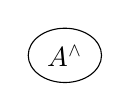
\begin{tikzpicture}[baseline=(n.base)]\node[draw,ellipse,inner sep=3pt] (n) {$A^{\wedge}$};\end{tikzpicture}}}
initial element \var{\xout{of}}{}{typewriter deletion}{ps_134-3_043-v0004} $\emptyset$ of (Cat) in the initial element $\emptyset$ of $A^{\hand{\wedge}}$ ), it follows
$e_o \hand{\cap} e_1 = \emptyset$ .

It's worth while having a look at what this \var{\deleted{\illegible{1}}}{}{deletion}{ps_134-3_043-v0005}\var{\inserted{object}}{\hand{object}}{insertion}{ps_134-3_043-v0006} just constructed is
like.  For this end,  let's note first that for any category \var{\inserted[typed]{C}}{C}{typed insertion}{ps_134-3_043-v0007}\hand{,} we have
a canonical bijection,  fonctorial in C
\[ \mathrm{Hom}(C, \hand{\Delta}_1) \hand{\xrightarrow{\sim}} \mathrm{Crib}(C) \hand{\simeq} \text{set of all subobjects of } e_{C^{\hand{\wedge}}} \ , \]
by associating to any functor $f\colon\ C \hand{\to} \hand{\Delta}_1$  the full subcategory $f^{-1}(\underline{e}_o)$ of
\margin{\diagram{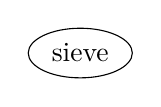
\begin{tikzpicture}[baseline=(n.base)]\node[draw,ellipse,inner sep=3pt] (n) {sieve};\end{tikzpicture}}}
C,  which clearly is a ``crible''\var{\inserted{[=sieve]}}{\hand{[=sieve]}}{insertion}{ps_134-3_043-v0008} in C.  Thus we get,  for a $\hand{\in}$ Ob A
\[ I(a) \hand{\simeq} \mathrm{Crib}(A_{/a}) \quad \hand{(}\text{subobjects of a in } A^{\hand{\wedge}}\hand{)}. \]
M\var{\over{\unsure{Q}}{o}}{\hand{o}}{writing over}{ps_134-3_043-v0009}re generally,  we deduce from this,  for any F $\hand{\in}$ Ob $A^{\hand{\wedge}}$:
\[ \mathrm{Hom}(F,I) = \hand{\Gamma}(I_F = I\mathrm{x}F \ / \ F) = \text{ set of all subobjects of } F\hand{,} \]
in other words, the object I is defined intrinsically in the topos $A^{\hand{\wedge}}$\hand{/}(up
to unique isomorphism)  as the ``\uline{Lawvere element}''  representing the functor
$F \hand{\mapsto}$ set of subobjects of F ,  generalizing the functor  $F \hand{\mapsto \mathfrak{P}}(F)$ in the
category of sets (namely sheaves over the one-point topos)\hand{,} \var{\inserted{(represented by the two-point set $\{0,1\}$.)}}{\hand{(represented by the two-point set $\{0,1\}$.)}}{insertion}{ps_134-3_043-v0010} The  condition
$e_o \hand{\cap} e_1 = \emptyset_{\hand{\mathcal{A}}}$  is automatic in any topos $\hand{\mathcal{A}}$, provided $\hand{\mathcal{A}}$ is not the ``empty
topos''  namely corresponding to a category of sheaves equivalent to a one-%
point category. \var{\deleted{Thus The condition  T 3' )  deduced from  T 3) by being
specific about the present choice of $(I,e_o,e_1)$ ,  is equivalent to T 3)
when T 1) and T 2) are satisfied,  and \xout{has the advantage} means simply that}}{}{deletion}{ps_134-3_043-v0011}

%% END SOURCE ps_134-3_043
\ifnum\EditionMode=1
\psapparatusstart
\psentry{ps_134-3_043-v0001}{1}{typed insertion}{\inserted[typed]{ly small in any case.)}}{ly small in any case.)}{The typed insertion is incorporated at its indicated position; insertion brackets leave the running text.}
\psentry{ps_134-3_043-v0002}{2}{writing over}{\over{\illegible{1}}{3}}{\hand{3}}{The superposed handwritten reading replaces the underlying reading.}
\psentry{ps_134-3_043-v0003}{3}{typewriter deletion}{\xout{x}}{}{The typewriter strikes out this material; it leaves the corrected running text.}
\psentry{ps_134-3_043-v0004}{4}{typewriter deletion}{\xout{of}}{}{The typewriter strikes out this material; it leaves the corrected running text.}
\psentry{ps_134-3_043-v0005}{5}{deletion}{\deleted{\illegible{1}}}{}{The author cancels this material by hand; it leaves the corrected running text.}
\psentry{ps_134-3_043-v0006}{6}{insertion}{\inserted{object}}{\hand{object}}{The handwritten insertion is incorporated at its indicated position; insertion brackets leave the running text.}
\psentry{ps_134-3_043-v0007}{7}{typed insertion}{\inserted[typed]{C}}{C}{The typed insertion is incorporated at its indicated position; insertion brackets leave the running text.}
\psentry{ps_134-3_043-v0008}{8}{insertion}{\inserted{[=sieve]}}{\hand{[=sieve]}}{The handwritten insertion is incorporated at its indicated position; insertion brackets leave the running text.}
\psentry{ps_134-3_043-v0009}{9}{writing over}{\over{\unsure{Q}}{o}}{\hand{o}}{The superposed handwritten reading replaces the underlying reading.}
\psentry{ps_134-3_043-v0010}{10}{insertion}{\inserted{(represented by the two-point set $\{0,1\}$.)}}{\hand{(represented by the two-point set $\{0,1\}$.)}}{The handwritten insertion is incorporated at its indicated position; insertion brackets leave the running text.}
\psentry{ps_134-3_043-v0011}{11}{deletion}{\deleted{Thus The condition  T 3' )  deduced from  T 3) by being
specific about the present choice of $(I,e_o,e_1)$ ,  is equivalent to T 3)
when T 1) and T 2) are satisfied,  and \xout{has the advantage} means simply that}}{}{The author cancels this material by hand; it leaves the corrected running text.}
\psapparatusend
\fi
\pssource{ps_134-3_044}{134-3/44}{https://grothendieck.umontpellier.fr/web/viewer.html?file=../134-3.pdf\#page=45}
\psnumber{ps_134-3_044-v0001}{1}
\psnumber{ps_134-3_044-v0002}{2}
\psnumber{ps_134-3_044-v0003}{3}
\psnumber{ps_134-3_044-v0004}{4}
\psnumber{ps_134-3_044-v0005}{5}
\psnumber{ps_134-3_044-v0006}{6}
\psnumber{ps_134-3_044-v0007}{7}
\psnumber{ps_134-3_044-v0008}{8}
\psnumber{ps_134-3_044-v0009}{9}
\psnumber{ps_134-3_044-v0010}{10}
\psnumber{ps_134-3_044-v0011}{11}
\psnumber{ps_134-3_044-v0012}{12}
\psnumber{ps_134-3_044-v0013}{13}
\psnumber{ps_134-3_044-v0014}{14}
\psnumber{ps_134-3_044-v0015}{15}
\psnumber{ps_134-3_044-v0016}{16}
\psnumber{ps_134-3_044-v0017}{17}
\psnumber{ps_134-3_044-v0018}{18}
%% BEGIN SOURCE ps_134-3_044
% Pursuing Stacks (cotes 134-2 to 134-8): archive cote 134-3, site page 44 (PDF page 45), typescript page 44.
% typescript. Draft compared: ps2.tex:2178-2237.
% AI-transcribed by Claude Opus 5.5 (claude-opus-5-5, adaptive thinking, effort high), Message Batches API, batch ps1 (msgbatch_01Rv5hCaNTtUt4JHx1yqoHPL), 2026-11-12; image review recorded in records/CHECK_DECISIONS_134_3_4.tsv.
\scanpage{134-3/44}
\mspage{44}
\var{\xout{For any topos.}}{}{typewriter deletion}{ps_134-3_044-v0001}
There is a strong temptation now to diverge from test categories,\hand{\textbackslash}to
\margin{\unsure{--}}expanding on intrinsic versions of conditions  T 1) to T 3) for any topos,
and extract a notion of a (strictly) modelizing topos,  generalizing the
``elementary \var{\xout{\unsure{topos}}}{}{typewriter deletion}{ps_134-3_044-v0002}\var{\inserted[typed]{modelizers''}}{modelizers''}{typed insertion}{ps_134-3_044-v0003} $A^{\hand{\wedge}}$ defined by strict test categories A.  But it seems
more to the point for the time being looking more closely to the one condi-%
tion,  namely T 2),  which does not appear so far as necessary for A being
a test category  -  and I suspect it is \uline{not} necessary indeed,  as no idea
occured to me how to deduce it\hand{(}\var{\inserted{34}}{\hand{34}}{insertion}{ps_134-3_044-v0004}\var{\xout{\illegible{1}}}{}{typewriter deletion}{ps_134-3_044-v0005}\hand{)}. ( I have no idea of how to make a coun-%
terexample though,  as I don't see any other way to check a category A is
a test category,  except precisely using \var{\xout{the}}{}{typewriter deletion}{ps_134-3_044-v0006}\var{\inserted[typed]{yesterday's}}{yesterday's}{typed insertion}{ps_134-3_044-v0007} criterion via T 1\hand{)}to T 3\hand{)}.\hand{)}
Still I want to emphasize about the fact that T 2) \uline{is indeed a very natural}
\uline{condition}.  In this connection,  it is timely to remember that in the cate-%
\margin{\diagram{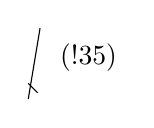
\begin{tikzpicture}[baseline=(n.base)]\draw (0,-.35)--(.15,.55);\draw (0,-.15)--(.12,-.27);\node[anchor=west] (n) at (.28,.18) {(!35)};\end{tikzpicture}}}gory (Hot),  finite direct and inverse limits exist\var{\deleted{\illegible{1}}}{}{deletion}{ps_134-3_044-v0008}(and even infinite one
I guess,  but I feel I'll have to be a little careful about these ...).
T\hand{h}e existence of such limits,  in terms of the description of (Hot) as a
category of fractions of (Cat),  does'nt seem at all a trivial fact,  for
the time being I'll admit it as \var{\xout{a}}{}{typewriter deletion}{ps_134-3_044-v0009} ``well known'' (\var{\xout{in}}{}{typewriter deletion}{ps_134-3_044-v0010}\var{\inserted[typed]{from}}{from}{typed insertion}{ps_134-3_044-v0011} the semisimplicial set-%
up,  say),  and probably come back upon this with some care later.  Now if
\var{\xout{a}}{}{typewriter deletion}{ps_134-3_044-v0012} (M,W) is any modelizer,  hence endowed with a localization functor
\[ M \hand{\longrightarrow} (\mathrm{Hot}) \ , \]
it is surely not irrelevant to ask about which limits this functor commu-%
tes with,  and study the case with care.  Thus in no \var{\inserted[typed]{practical}}{practical}{typed insertion}{ps_134-3_044-v0013} example I know of
does this functor commute with binary amalgamated sums o\var{\over{f}{r}}{\hand{r}}{writing over}{ps_134-3_044-v0014} \var{\inserted{with}}{\hand{with}}{insertion}{ps_134-3_044-v0015} fibere\var{\over{a}{d}}{\hand{d}}{writing over}{ps_134-3_044-v0016} products,
without an extra condition on at least one of the two arrows involved in
M  -  a condition of the type that one of these is a mo\var{\over{i}{n}}{\hand{n}}{writing over}{ps_134-3_044-v0017}omorphism or a
c\var{\over{\unsure{o}}{o}}{\hand{o}}{writing over}{ps_134-3_044-v0018}fibration (for co-products),  or a fibration (for products).  However,
in all cases known,  it seems that the functor commutes to (finite,  say)
sums and products.  For sums,  it really seems hard to make a sense out of
a localizing functor  M\hand{$\longrightarrow$}(Hot),  namely playing a ``model'' game,  without
the functor commuting at the very least to these !  In this respect,  it
is reassuring to notice that for any category A ,  the associated functors
$i_A$, $j_A$ between  $A^{\hand{\wedge}}$ and (Cat) do indeed both commute with (arbitrary) sums
-  which of course is trivial anyhow for $i_A$ (commuting to arbitrary direct
limits),  and easily checked for $j_A$ (who apparently does not commute to any
other type of direct limits,  but of course commutes with arbitrary inverse
limits).  Now for products too,  it is current use to look at products of
``models'' for homotopy types,  as models for the product type  -  so much so
that this fact is surely tacitly used everywhere\hand{,} without any feeling of
a need to comment.  It seems too that any categories M which one has looked
at so far for possible use as a category of ``models'' in one sense or other

%% END SOURCE ps_134-3_044
\ifnum\EditionMode=1
\psapparatusstart
\psentry{ps_134-3_044-v0001}{1}{typewriter deletion}{\xout{For any topos.}}{}{The typewriter strikes out this material; it leaves the corrected running text.}
\psentry{ps_134-3_044-v0002}{2}{typewriter deletion}{\xout{\unsure{topos}}}{}{The typewriter strikes out this material; it leaves the corrected running text.}
\psentry{ps_134-3_044-v0003}{3}{typed insertion}{\inserted[typed]{modelizers''}}{modelizers''}{The typed insertion is incorporated at its indicated position; insertion brackets leave the running text.}
\psentry{ps_134-3_044-v0004}{4}{insertion}{\inserted{34}}{\hand{34}}{The handwritten insertion is incorporated at its indicated position; insertion brackets leave the running text.}
\psentry{ps_134-3_044-v0005}{5}{typewriter deletion}{\xout{\illegible{1}}}{}{The typewriter strikes out this material; it leaves the corrected running text.}
\psentry{ps_134-3_044-v0006}{6}{typewriter deletion}{\xout{the}}{}{The typewriter strikes out this material; it leaves the corrected running text.}
\psentry{ps_134-3_044-v0007}{7}{typed insertion}{\inserted[typed]{yesterday's}}{yesterday's}{The typed insertion is incorporated at its indicated position; insertion brackets leave the running text.}
\psentry{ps_134-3_044-v0008}{8}{deletion}{\deleted{\illegible{1}}}{}{The author cancels this material by hand; it leaves the corrected running text.}
\psentry{ps_134-3_044-v0009}{9}{typewriter deletion}{\xout{a}}{}{The typewriter strikes out this material; it leaves the corrected running text.}
\psentry{ps_134-3_044-v0010}{10}{typewriter deletion}{\xout{in}}{}{The typewriter strikes out this material; it leaves the corrected running text.}
\psentry{ps_134-3_044-v0011}{11}{typed insertion}{\inserted[typed]{from}}{from}{The typed insertion is incorporated at its indicated position; insertion brackets leave the running text.}
\psentry{ps_134-3_044-v0012}{12}{typewriter deletion}{\xout{a}}{}{The typewriter strikes out this material; it leaves the corrected running text.}
\psentry{ps_134-3_044-v0013}{13}{typed insertion}{\inserted[typed]{practical}}{practical}{The typed insertion is incorporated at its indicated position; insertion brackets leave the running text.}
\psentry{ps_134-3_044-v0014}{14}{writing over}{\over{f}{r}}{\hand{r}}{The superposed handwritten reading replaces the underlying reading.}
\psentry{ps_134-3_044-v0015}{15}{insertion}{\inserted{with}}{\hand{with}}{The handwritten insertion is incorporated at its indicated position; insertion brackets leave the running text.}
\psentry{ps_134-3_044-v0016}{16}{writing over}{\over{a}{d}}{\hand{d}}{The superposed handwritten reading replaces the underlying reading.}
\psentry{ps_134-3_044-v0017}{17}{writing over}{\over{i}{n}}{\hand{n}}{The superposed handwritten reading replaces the underlying reading.}
\psentry{ps_134-3_044-v0018}{18}{writing over}{\over{\unsure{o}}{o}}{\hand{o}}{The superposed handwritten reading replaces the underlying reading.}
\psapparatusend
\fi
\pssource{ps_134-3_045}{134-3/45}{https://grothendieck.umontpellier.fr/web/viewer.html?file=../134-3.pdf\#page=46}
\psnumber{ps_134-3_045-v0001}{1}
\psnumber{ps_134-3_045-v0002}{2}
\psnumber{ps_134-3_045-v0003}{3}
\psnumber{ps_134-3_045-v0004}{4}
\psnumber{ps_134-3_045-v0005}{5}
\psnumber{ps_134-3_045-v0006}{6}
\psnumber{ps_134-3_045-v0007}{7}
\psnumber{ps_134-3_045-v0008}{8}
\psnumber{ps_134-3_045-v0009}{9}
\psnumber{ps_134-3_045-v0010}{10}
\psnumber{ps_134-3_045-v0011}{11}
\psnumber{ps_134-3_045-v0012}{12}
\psnumber{ps_134-3_045-v0013}{13}
\psnumber{ps_134-3_045-v0014}{14}
\psnumber{ps_134-3_045-v0015}{15}
\psnumber{ps_134-3_045-v0016}{16}
%% BEGIN SOURCE ps_134-3_045
% Pursuing Stacks (cotes 134-2 to 134-8): archive cote 134-3, site page 45 (PDF page 46), typescript page 45.
% typescript. Draft compared: ps2.tex:2225-2293.
% AI-transcribed by Claude Opus 5.5 (claude-opus-5-5, adaptive thinking, effort high), Message Batches API, batch ps1 (msgbatch_01Rv5hCaNTtUt4JHx1yqoHPL), 2026-11-12; image review recorded in records/CHECK_DECISIONS_134_3_4.tsv.
\scanpage{134-3/45}
\mspage{45}
for homotopy types,  for  instance set-theoretic realisations of some speci-%
fied algebraic structure species, or topological spaces,  and the like,
do admit arbitrary direct and inverse limits,  and surely \var{\xout{finite}}{}{typewriter deletion}{ps_134-3_045-v0001} sums and
products therefore,  so that the question of commutation of the localizati-%
on functor \var{\inserted{to these}}{\hand{to these}}{insertion}{ps_134-3_045-v0002} arises indeed and is felt to be important.  Possibly so impor-%
tant even,  that the notion I introduced of a ``modelizer'' should take this
into account,  and be strengthened to the effect that the canonical functor
$M\hand{\longrightarrow}$(Hot)  should commute at least to finite sums and products,  and possib-%
ly even to infinite ones (\var{\xout{this}}{}{typewriter deletion}{ps_134-3_045-v0003} \var{\inserted[typed]{whether}}{whether}{typed insertion}{ps_134-3_045-v0004} \var{\inserted{the latter}}{\hand{the latter}}{insertion}{ps_134-3_045-v0005} will have to be looked up with care).  I'll
admit \var{\inserted{provisionally}}{\hand{provisionally}}{insertion}{ps_134-3_045-v0006} that in (Hot),  finite sums and products can be described in terms of
the corresponding operations in (Cat),  namely that the canonical functor
(going with our very definition of (Hot) as a localization of (Cat))
\[ (\mathrm{Cat}) \hand{\longrightarrow} (\mathrm{Hot}) \]
commutes with finite (presumably even infinite) sums and products.\hand{(\unsure{35})} This is
indeed reasonable,  in view of the fact that the Nerve functor
\[ (\mathrm{Cat}) \hand{\longrightarrow} \hand{\Delta}^{\hand{\wedge}} = (\mathrm{Ss\ sets}) \]
does commute to sums and products.

In the case of a test category\var{\xout{,}}{}{typewriter deletion}{ps_134-3_045-v0007} A and the corresponding elementary mode-%
lizer $A^{\hand{\wedge}}$,  the corresponding localizing functor is the compositum
\[ A^{\hand{\wedge}} \overset{i_A}{\hand{\longrightarrow}} (\mathrm{Cat}) \hand{\longrightarrow} (\mathrm{Hot}) \ , \]
which therefore commutes with finite (presumably even infinite) sums automa-%
tically,  because $\hand{i}_A$ does.  Commutation with finite \uline{products} though does
not look automatic.  The \var{\xout{fact that}}{}{typewriter deletion}{ps_134-3_045-v0008} property of commutation with final
elements is OK and is nothing but condition T 1),  which we saw is necessa-%
ry for A to be a test category.  Thus remains the question of commutation
with binary products,  which boils down to the following condition,  for
any two elements  F and G in $A^{\hand{\wedge}}$:
\[ i_A(F\mathrm{x}G) \hand{\longrightarrow} i_A(F)\mathrm{x}i_A(G) \quad \text{should be a weak equivalence} \]
i.e.
\[ (*) \qquad A_{/F\mathrm{x}G} \hand{\longrightarrow} A_{/F}\ \mathrm{x}\ A_{/G} \quad \text{a weak equivalence .} \]
\var{\xout{a weak equivalence}}{}{typewriter deletion}{ps_134-3_045-v0009} This now implies condition T 2),  as we see taking
$F = a$ , $G = b$ ,  \var{\xout{and}}{}{typewriter deletion}{ps_134-3_045-v0010} in which case the condition \var{\xout{boils down to}}{}{typewriter deletion}{ps_134-3_045-v0011} \var{\inserted[typed]{(*) just means}}{(*) just means}{typed insertion}{ps_134-3_045-v0012} asphericity
of  $a\mathrm{x}b$ in $A^{\hand{\wedge}}$ namely  T 2 .  To be happy,  we have still to show that
conversely,  (T 2) implies (*)  for any F,G.  As usual,  it implies even the
stronger condition that the functor in question is aspheric,  which by the
standar\var{\over{t}{d}}{\hand{d}}{writing over}{ps_134-3_045-v0013} criterion  (page 38)  just means that the categories $A_{/a\mathrm{x}b}$
(for a,b in A, \var{\inserted{and}}{\hand{and}}{insertion}{ps_134-3_045-v0014} such \var{\inserted{moreover}}{\hand{moreover}}{insertion}{ps_134-3_045-v0015} that F(a) and G(b) non empty, \var{\inserted{but}}{\hand{but}}{insertion}{ps_134-3_045-v0016} never mind) are aspheric.

Everything turns out just perfect  -  it seems worthwhile to summarize
it in one theorem:

%% END SOURCE ps_134-3_045
\ifnum\EditionMode=1
\psapparatusstart
\psentry{ps_134-3_045-v0001}{1}{typewriter deletion}{\xout{finite}}{}{The typewriter strikes out this material; it leaves the corrected running text.}
\psentry{ps_134-3_045-v0002}{2}{insertion}{\inserted{to these}}{\hand{to these}}{The handwritten insertion is incorporated at its indicated position; insertion brackets leave the running text.}
\psentry{ps_134-3_045-v0003}{3}{typewriter deletion}{\xout{this}}{}{The typewriter strikes out this material; it leaves the corrected running text.}
\psentry{ps_134-3_045-v0004}{4}{typed insertion}{\inserted[typed]{whether}}{whether}{The typed insertion is incorporated at its indicated position; insertion brackets leave the running text.}
\psentry{ps_134-3_045-v0005}{5}{insertion}{\inserted{the latter}}{\hand{the latter}}{The handwritten insertion is incorporated at its indicated position; insertion brackets leave the running text.}
\psentry{ps_134-3_045-v0006}{6}{insertion}{\inserted{provisionally}}{\hand{provisionally}}{The handwritten insertion is incorporated at its indicated position; insertion brackets leave the running text.}
\psentry{ps_134-3_045-v0007}{7}{typewriter deletion}{\xout{,}}{}{The typewriter strikes out this material; it leaves the corrected running text.}
\psentry{ps_134-3_045-v0008}{8}{typewriter deletion}{\xout{fact that}}{}{The typewriter strikes out this material; it leaves the corrected running text.}
\psentry{ps_134-3_045-v0009}{9}{typewriter deletion}{\xout{a weak equivalence}}{}{The typewriter strikes out this material; it leaves the corrected running text.}
\psentry{ps_134-3_045-v0010}{10}{typewriter deletion}{\xout{and}}{}{The typewriter strikes out this material; it leaves the corrected running text.}
\psentry{ps_134-3_045-v0011}{11}{typewriter deletion}{\xout{boils down to}}{}{The typewriter strikes out this material; it leaves the corrected running text.}
\psentry{ps_134-3_045-v0012}{12}{typed insertion}{\inserted[typed]{(*) just means}}{(*) just means}{The typed insertion is incorporated at its indicated position; insertion brackets leave the running text.}
\psentry{ps_134-3_045-v0013}{13}{writing over}{\over{t}{d}}{\hand{d}}{The superposed handwritten reading replaces the underlying reading.}
\psentry{ps_134-3_045-v0014}{14}{insertion}{\inserted{and}}{\hand{and}}{The handwritten insertion is incorporated at its indicated position; insertion brackets leave the running text.}
\psentry{ps_134-3_045-v0015}{15}{insertion}{\inserted{moreover}}{\hand{moreover}}{The handwritten insertion is incorporated at its indicated position; insertion brackets leave the running text.}
\psentry{ps_134-3_045-v0016}{16}{insertion}{\inserted{but}}{\hand{but}}{The handwritten insertion is incorporated at its indicated position; insertion brackets leave the running text.}
\psapparatusend
\fi
\pssource{ps_134-3_046}{134-3/46}{https://grothendieck.umontpellier.fr/web/viewer.html?file=../134-3.pdf\#page=47}
\psnumber{ps_134-3_046-v0001}{1}
\psnumber{ps_134-3_046-v0002}{2}
\psnumber{ps_134-3_046-v0003}{3}
\psnumber{ps_134-3_046-v0004}{4}
\psnumber{ps_134-3_046-v0005}{5}
\psnumber{ps_134-3_046-v0006}{6}
\psnumber{ps_134-3_046-v0007}{7}
\psnumber{ps_134-3_046-v0008}{8}
\psnumber{ps_134-3_046-v0009}{9}
\psnumber{ps_134-3_046-v0010}{10}
\psnumber{ps_134-3_046-v0011}{11}
\psnumber{ps_134-3_046-v0012}{12}
\psnumber{ps_134-3_046-v0013}{13}
%% BEGIN SOURCE ps_134-3_046
% Pursuing Stacks (cotes 134-2 to 134-8): archive cote 134-3, site page 46 (PDF page 47), typescript page 46.
% typescript. Draft compared: ps2.tex:2276-2337.
% AI-transcribed by Claude Opus 5.5 (claude-opus-5-5, adaptive thinking, effort high), Message Batches API, batch ps1 (msgbatch_01Rv5hCaNTtUt4JHx1yqoHPL), 2026-11-12; image review recorded in records/CHECK_DECISIONS_134_3_4.tsv.
\scanpage{134-3/46}
\mspage{46}

\uline{Theorem}: Let A be an essentially small category, and consider the compo\var{\xout{si}}{}{typewriter deletion}{ps_134-3_046-v0001}\var{\inserted[typed]{sed}}{sed}{typed insertion}{ps_134-3_046-v0002}
\var{\xout{tion}}{}{typewriter deletion}{ps_134-3_046-v0003} functor
\[ m_A : A^{\hand{\wedge}} \overset{i_A}{\hand{\longrightarrow}} (Cat)\hand{\longrightarrow}(Hot) , \]
where $i_A(F) = A_{/F}$ for any $F \hand{\in} \mathrm{Ob}\, A^{\hand{\wedge}}$, and where (Cat)\hand{$\longrightarrow$}(Hot) is the
canonical functor from (Cat) into the localized category with respect to
weak equivalences. The following conditions are equivalent:
\margin{\unsure{9.4. Presumably}}(i) The functor $m_A$ commutes with finite products, and is a localiza-
tion functor, i.e. induces an equivalence $W_A^{-1}A^{\hand{\wedge}} \hand{\xrightarrow{\approx}}$(Hot), where
$W_A$ is the set of weak equivalences in $A^{\hand{\wedge}}$, namely arrows transfor-
med into weak equivalences by $i_A$ \hand{(*37)}. \margin{cf remark 3 p.174 -- is not strong enough}
\margin{\unsure{we'll have to add that $j_A = i_A^*$ is model preserving, cf remark 3 on p. 174}}
(ii) The functor $i_A$ and it's right adjoint $j_A$ \var{\deleted{\xout{def}}}{}{deletion}{ps_134-3_046-v0004} define functors bet-
ween $W_A^{-1}A^{\hand{\wedge}}$ and (Hot) = $W^{-1}$(Cat) (\var{\inserted{thus,}}{\hand{thus,}}{insertion}{ps_134-3_046-v0005} $j_A$ \var{\inserted{should}}{\hand{should}}{insertion}{ps_134-3_046-v0006} transform\var{\deleted{ing}}{}{deletion}{ps_134-3_046-v0007} weak equiva-
lences of (Cat) into weak equivalences of $A^{\hand{\wedge}}$) which are \uline{quasi-in-}%
\uline{verse} to each other, the adjunction morphisms for this pair being
deduced from the adjunction morphisms for the pair $i_A, j_A$ . Moreover
\var{\inserted[typed]{the functor $m_A$ commutes with finite products.}}{the functor $m_A$ commutes with finite products.}{typed insertion}{ps_134-3_046-v0008}
(iii) The category A satisfies the \var{\xout{following}}{}{typewriter deletion}{ps_134-3_046-v0009} conditions T 1 to T 3
(page 39).

I could go on with two or three more equivalent conditions, which
could be expressed intrinsically in terms of the topos $A^{\hand{\wedge}}$ and make sense
(and are equivalent) for any topos, along the lines of the reflections of
p. 43 and of yesterday\var{\xout{s}}{}{typewriter deletion}{ps_134-3_046-v0010} . But I'll still refrain for the time being\hand{!}

In the proof of the theorem above, I did not make use of semi-simpli\var{\xout{\illegible{1}}}{}{typewriter deletion}{ps_134-3_046-v0011}%
cial techniques nor of any known results about (Hot), with the only excep-%
tion of the assumption (a fact, I daresay, but not proved for the time be-%
ing in the present framework, without reference to semi-simplicial theory
say) that the canonical functor (Cat)\hand{$\longrightarrow$}(Hot) commutes with binary pro-%
ducts. We could have avoided this assumption, by slightly changing the
statement of the theorem, the condition that $m_A$ commute with finite pro\var{\deleted{\xout{du}}}{}{deletion}{ps_134-3_046-v0012}\hand{-}%
ducts \var{\inserted[typed]{in (i) and (ii)}}{in (i) and (ii)}{typed insertion}{ps_134-3_046-v0013} being replaced by the assumption that $i_A$ commute with finite products
``up to weak equivalence'', as made explicit in (*) above for the case of
binary products (which are enough of course).

I suspect that the notion of a test category in the initial, wider
sense will be of no use any longer, and therefore I will reserve this na-%

%% END SOURCE ps_134-3_046
\ifnum\EditionMode=1
\psapparatusstart
\psentry{ps_134-3_046-v0001}{1}{typewriter deletion}{\xout{si}}{}{The typewriter strikes out this material; it leaves the corrected running text.}
\psentry{ps_134-3_046-v0002}{2}{typed insertion}{\inserted[typed]{sed}}{sed}{The typed insertion is incorporated at its indicated position; insertion brackets leave the running text.}
\psentry{ps_134-3_046-v0003}{3}{typewriter deletion}{\xout{tion}}{}{The typewriter strikes out this material; it leaves the corrected running text.}
\psentry{ps_134-3_046-v0004}{4}{deletion}{\deleted{\xout{def}}}{}{The author cancels this material by hand; it leaves the corrected running text.}
\psentry{ps_134-3_046-v0005}{5}{insertion}{\inserted{thus,}}{\hand{thus,}}{The handwritten insertion is incorporated at its indicated position; insertion brackets leave the running text.}
\psentry{ps_134-3_046-v0006}{6}{insertion}{\inserted{should}}{\hand{should}}{The handwritten insertion is incorporated at its indicated position; insertion brackets leave the running text.}
\psentry{ps_134-3_046-v0007}{7}{deletion}{\deleted{ing}}{}{The author cancels this material by hand; it leaves the corrected running text.}
\psentry{ps_134-3_046-v0008}{8}{typed insertion}{\inserted[typed]{the functor $m_A$ commutes with finite products.}}{the functor $m_A$ commutes with finite products.}{The typed insertion is incorporated at its indicated position; insertion brackets leave the running text.}
\psentry{ps_134-3_046-v0009}{9}{typewriter deletion}{\xout{following}}{}{The typewriter strikes out this material; it leaves the corrected running text.}
\psentry{ps_134-3_046-v0010}{10}{typewriter deletion}{\xout{s}}{}{The typewriter strikes out this material; it leaves the corrected running text.}
\psentry{ps_134-3_046-v0011}{11}{typewriter deletion}{\xout{\illegible{1}}}{}{The typewriter strikes out this material; it leaves the corrected running text.}
\psentry{ps_134-3_046-v0012}{12}{deletion}{\deleted{\xout{du}}}{}{The author cancels this material by hand; it leaves the corrected running text.}
\psentry{ps_134-3_046-v0013}{13}{typed insertion}{\inserted[typed]{in (i) and (ii)}}{in (i) and (ii)}{The typed insertion is incorporated at its indicated position; insertion brackets leave the running text.}
\psapparatusend
\fi
\pssource{ps_134-3_047}{134-3/47}{https://grothendieck.umontpellier.fr/web/viewer.html?file=../134-3.pdf\#page=48}
\psnumber{ps_134-3_047-v0001}{1}
\psnumber{ps_134-3_047-v0002}{2}
\psnumber{ps_134-3_047-v0003}{3}
\psnumber{ps_134-3_047-v0004}{4}
\psnumber{ps_134-3_047-v0005}{5}
\psnumber{ps_134-3_047-v0006}{6}
\psnumber{ps_134-3_047-v0007}{7}
\psnumber{ps_134-3_047-v0008}{8}
\psnumber{ps_134-3_047-v0009}{9}
\psnumber{ps_134-3_047-v0010}{10}
\psnumber{ps_134-3_047-v0011}{11}
%% BEGIN SOURCE ps_134-3_047
% Pursuing Stacks (cotes 134-2 to 134-8): archive cote 134-3, site page 47 (PDF page 48), typescript page 47.
% typescript. Draft compared: ps2.tex:2327-2401.
% AI-transcribed by Claude Opus 5.5 (claude-opus-5-5, adaptive thinking, effort high), Message Batches API, batch ps1 (msgbatch_01Rv5hCaNTtUt4JHx1yqoHPL), 2026-11-12; image review recorded in records/CHECK_DECISIONS_134_3_4.tsv.
\scanpage{134-3/47}
\mspage{47}
me to the \uline{strict} case henceforth,  namely to the case of categories satis-%
fying the equivalent conditions of the theorem above\hand{(38)}. Accordingly, I'll
call \uline{``elementary modelizer''} any category \var{\inserted{$\mathcal{A}$}}{\hand{$\mathcal{A}$}}{insertion}{ps_134-3_047-v0001} equivalent to a category $A^{\hand{\wedge}}$,
with A a test category.  Such a category will be always considered as a mo-%
delizer, of course,  with the usual notion of weak equivalence W\hand{$\subset$}F\var{\over{l}{l}}{\hand{l}}{writing over}{ps_134-3_047-v0002}(\hand{$\mathcal{A}$}),
namely \var{\inserted[typed]{of}}{of}{typed insertion}{ps_134-3_047-v0003} a ``map''  F\hand{$\to$}G in \hand{$\mathcal{A}$} such that the corresponding morphism for the
induced topoi is a weak equivalence.  The \var{\xout{topos}}{}{typewriter deletion}{ps_134-3_047-v0004} category \hand{$\mathcal{A}$} is an elementa-%
ry modelizer,  therefore,  iff it satisfies the following conditions:

a) \hand{$\mathcal{A}$} is equivalent to a category $A^{\hand{\wedge}}$ with a small \hand{$A$,} which amounts to
saying that \hand{$\mathcal{A}$} is a topos,  and has sufficiently many ``essential points''
namely ``points'' such that the corresponding fiber-functor \hand{$\mathcal{A}\to$} (Ens) commu-%
tes with arbitrary products  -  i.e. there exists a conservative family
of functors  \hand{$\mathcal{A}\to$} (Ens)  which commute to arbitrary direct and inverse
limits\hand{\unsure{.}} (Cf SGA 4 IV 7.5.).

b)  The pair (\hand{$\mathcal{A}$} ,W) is modelizing (where W \hand{$\subset$} F\var{\over{l}{l}}{\hand{l}}{writing over}{ps_134-3_047-v0005}(\hand{$\mathcal{A}$}) is the set of weak
equivalences),  i.e. the category  $W^{-1}$\hand{$\mathcal{A}$}  is equivalent to (Hot).

c)  The canonical functor  \hand{$\mathcal{A}\to$}(Hot)  (or, equivalently, \hand{$\mathcal{A}\to$} $W^{-1}$\hand{$\mathcal{A}$})
commutes with finite products (or, equivalently,  with binary products -
that it commutes with final elements follows already from a),b)).

As I felt insistently since yesterday,  there is a very pretty notion
of a ``modelizing topos'' generalizing the notion of an elementary modelizer,
where \hand{$\mathcal{A}$} is a topos but not necessarily equivalent to one of the type $A^{\hand{\wedge}}$
-  but \var{\xout{admitting}}{}{typewriter deletion}{ps_134-3_047-v0006} where \var{\inserted{however}}{\hand{however}}{insertion}{ps_134-3_047-v0007} the aspheric (= ``contractible'' ) objects form a
generating family (which generalizes the condition \hand{$\mathcal{A}\simeq$}$A^{\hand{\wedge}}$\var{\unsure{\xout{x}}}{}{typewriter deletion}{ps_134-3_047-v0008} ,which means
\margin{\diagram{\begin{tikzpicture}\draw[->] (.7,0)--(.2,0) .. controls (0,0) and (0,.2) .. (0,.4)--(0,1.2);\end{tikzpicture}}}that the O-connected projective elements of \hand{$\mathcal{A}$} form a generating family).
I'll come back upon this notion later I guess -  it is not the most urgent
thing for the time being ...

\margin{\diagram{\begin{tikzpicture}\draw[->] (.8,1.2)--(.2,1.2) .. controls (0,1.2) and (0,1.1) .. (0,.9)--(0,0);\end{tikzpicture}}}34.    I will now exploit the handy criterion  T 1) to T 3) for test catego%
ries, for constructing lots of such.  In all cases I have in mind at pre-%
sent,  the verification of  T 1) and T 3) is obvious,  they are consequenc\unsure{es}
indeed of the following stronger conditions:
T 1')  A has a final element e$_{A}$\var{\deleted{\illegible{1}}}{}{deletion}{ps_134-3_047-v0009}.
T 3')  There exists an element \var{\inserted[typed]{I=}}{I=}{typed insertion}{ps_134-3_047-v0010}I$_{A}$ in A, and two sections \hand{$e_0,e_1$} of I over
e = e$_{A}$
\[ \hand{\delta_0,\delta_1} :\ e \hand{\to} I \ , \]
such that the corresponding subobjects e$_0$,e$_1$ of I satisfy \var{\xout{x}}{}{typewriter deletion}{ps_134-3_047-v0011}
\[ e_0\hand{\cap}e_1 = \emptyset_{A^{\hand{\wedge}}} \ , \]
namely that for any a \hand{$\in$}Ob A , if p$_{a}$ : a \hand{$\to$}e is the projection, we
have
\[ \hand{\delta_0 p_a \neq \delta_1 p_a} . \]

%% END SOURCE ps_134-3_047
\ifnum\EditionMode=1
\psapparatusstart
\psentry{ps_134-3_047-v0001}{1}{insertion}{\inserted{$\mathcal{A}$}}{\hand{$\mathcal{A}$}}{The handwritten insertion is incorporated at its indicated position; insertion brackets leave the running text.}
\psentry{ps_134-3_047-v0002}{2}{writing over}{\over{l}{l}}{\hand{l}}{The superposed handwritten reading replaces the underlying reading.}
\psentry{ps_134-3_047-v0003}{3}{typed insertion}{\inserted[typed]{of}}{of}{The typed insertion is incorporated at its indicated position; insertion brackets leave the running text.}
\psentry{ps_134-3_047-v0004}{4}{typewriter deletion}{\xout{topos}}{}{The typewriter strikes out this material; it leaves the corrected running text.}
\psentry{ps_134-3_047-v0005}{5}{writing over}{\over{l}{l}}{\hand{l}}{The superposed handwritten reading replaces the underlying reading.}
\psentry{ps_134-3_047-v0006}{6}{typewriter deletion}{\xout{admitting}}{}{The typewriter strikes out this material; it leaves the corrected running text.}
\psentry{ps_134-3_047-v0007}{7}{insertion}{\inserted{however}}{\hand{however}}{The handwritten insertion is incorporated at its indicated position; insertion brackets leave the running text.}
\psentry{ps_134-3_047-v0008}{8}{typewriter deletion}{\unsure{\xout{x}}}{}{All material inside this wrapper is cancelled. Its original doubt and presentation remain in the diplomatic text and apparatus; no empty doubt mark or page label is inserted into the corrected running text.}
\psentry{ps_134-3_047-v0009}{9}{deletion}{\deleted{\illegible{1}}}{}{The author cancels this material by hand; it leaves the corrected running text.}
\psentry{ps_134-3_047-v0010}{10}{typed insertion}{\inserted[typed]{I=}}{I=}{The typed insertion is incorporated at its indicated position; insertion brackets leave the running text.}
\psentry{ps_134-3_047-v0011}{11}{typewriter deletion}{\xout{x}}{}{The typewriter strikes out this material; it leaves the corrected running text.}
\psapparatusend
\fi
\pssource{ps_134-3_048}{134-3/48}{https://grothendieck.umontpellier.fr/web/viewer.html?file=../134-3.pdf\#page=49}
\psnumber{ps_134-3_048-v0001}{1}
\psnumber{ps_134-3_048-v0002}{2}
\psnumber{ps_134-3_048-v0003}{3}
\psnumber{ps_134-3_048-v0004}{4}
\psnumber{ps_134-3_048-v0005}{5}
\psnumber{ps_134-3_048-v0006}{6}
\psnumber{ps_134-3_048-v0007}{7}
\psnumber{ps_134-3_048-v0008}{8}
\psnumber{ps_134-3_048-v0009}{9}
\psnumber{ps_134-3_048-v0010}{10}
\psnumber{ps_134-3_048-v0011}{11}
\psnumber{ps_134-3_048-v0012}{12}
\psnumber{ps_134-3_048-v0013}{13}
\psnumber{ps_134-3_048-v0014}{14}
\psnumber{ps_134-3_048-v0015}{15}
\psnumber{ps_134-3_048-v0016}{16}
\psnumber{ps_134-3_048-v0017}{17}
\psnumber{ps_134-3_048-v0018}{18}
\psnumber{ps_134-3_048-v0019}{19}
\psnumber{ps_134-3_048-v0020}{20}
\psnumber{ps_134-3_048-v0021}{21}
\psnumber{ps_134-3_048-v0022}{22}
%% BEGIN SOURCE ps_134-3_048
% Pursuing Stacks (cotes 134-2 to 134-8): archive cote 134-3, site page 48 (PDF page 49), typescript page 48.
% typescript. Draft compared: ps2.tex:2385-2457.
% AI-transcribed by Claude Opus 5.5 (claude-opus-5-5, adaptive thinking, effort high), Message Batches API, batch ps1 (msgbatch_01Rv5hCaNTtUt4JHx1yqoHPL), 2026-11-12; image review recorded in records/CHECK_DECISIONS_134_3_4.tsv.
\scanpage{134-3/48}
\mspage{\hand{48}}

Of course,  the element I  (playing the role of unit interval with
endpoints $e_o$,$e_1$) is by no means unique,  for instance it can be replaced
by any cartesian power $I^n$ $(n\hand{\geqslant} 1)$,  provided it is in \var{\over{A}{$A$}}{\hand{$A$}}{writing over}{ps_134-3_048-v0001}  -  or in the case
of A = \hand{$\Delta$}  we can take for I any \hand{$\Delta$}$_n$ $(n\hand{\geqslant} 1)$ and for \hand{$\delta$}$_o$ ,\hand{$\delta$}$_1$ any two \uline{distinct}
maps from e=\hand{$\Delta$}$_o$ to \hand{$\Delta$}$_n$ , instead of the usual choice \var{\xout{for}}{}{typewriter deletion}{ps_134-3_048-v0002} \hand{$\Delta$}$_1$ for I, and
corresponding \hand{$\delta$}$_o$ and \hand{$\delta$}$_1$ .  This high degree of arbitrar\var{\over{y}{i}}{\hand{i}}{writing over}{ps_134-3_048-v0003}ness in the choice
of I should be no surprise,  this was already one striking feature in Quil-%
len's theory of model categories.

There remains the asphericity condition (T 2)  for the categories
$A_{/axb}$ ,  with  a,b \hand{$\in$} Ob A ,  which is somewhat subtler.  There is one very
evident way though to insure this, namely assuming

T 2')  If a,b are in A,  so is axb  i.e. A is stable under binary products.

In other words,  putting together  T 1' and T 2',  \var{\xout{taking any categ}}{}{typewriter deletion}{ps_134-3_048-v0004} we
may \var{\xout{restrict}}{}{typewriter deletion}{ps_134-3_048-v0005} take categories (essential small) \uline{stable under finite products}
When such a category satisfies the mild extra condition T 3') above,  it
is a test category!  This is already an impressive bunch of test categories
For instance take any category \var{\inserted[typed]{C}}{C}{typed insertion}{ps_134-3_048-v0006}\var{\inserted[typed]{with}}{with}{typed insertion}{ps_134-3_048-v0007} \var{\xout{stable under}}{}{typewriter deletion}{ps_134-3_048-v0008} finite products and \var{\xout{for which}}{}{typewriter deletion}{ps_134-3_048-v0009}
for which there exist I,$e_o$,$e_1$ as in T 3'  -  never mind whether \hand{C} is essen-%
tially small,  for instance any "non empty" topos will do (taking for I
the Lawvere element for instance,  if no simpler choice comes to \var{\over{\illegible{1}}{m}}{\hand{m}}{writing over}{ps_134-3_048-v0010}ind).
Ta\var{\over{\unsure{k}}{k}}{\hand{k}}{writing over}{ps_134-3_048-v0011}e any subcategory \var{\inserted[typed]{A}}{A}{typed insertion}{ps_134-3_048-v0012} (full or not) stable \var{\xout{by}}{}{typewriter deletion}{ps_134-3_048-v0013}\var{\inserted[typed]{under}}{under}{typed insertion}{ps_134-3_048-v0014} finite products and containing
I and \hand{$\Delta$}$_o$ ,\hand{$\Delta$}$_1$ and where the  C-products are also A-products  -  for instan\var{\xout{c}}{}{typewriter deletion}{ps_134-3_048-v0015}
ce this is OK if A is full.  \var{Then A is a test category. \margin{\diagram{\begin{tikzpicture}\draw (0,0)--(.55,0)--(.66,.42)--(1.15,.42);\end{tikzpicture}}} The simplest choi-}{Then A is a test category.

The simplest choi-}{author paragraph break}{ps_134-3_048-v0016}%
ce her\var{\over{e}{e}}{\hand{e}}{writing over}{ps_134-3_048-v0017},  the smallest in any case,  is to take the subcategory made up
with all cartesian powers $I^n$ $(n\hand{\geqslant} 0)$.  We may take the full subcategory
made up with these elements,  but instead we may take,\var{\xout{as only arrows}}{}{typewriter deletion}{ps_134-3_048-v0018} still
more economically,  only the arrows
\[ I^n \hand{\rightarrow} I^m \]
whose \var{\inserted[typed]{m}}{m}{typed insertion}{ps_134-3_048-v0019} components  $I^n \hand{\rightarrow} I$ are each,  either a projection $pr_i$ $(1\hand{\leqslant} i\hand{\leqslant} n)$ or
of the form \hand{$\delta$}$_i$\hand{$($}$p_{I^n}$\hand{$)$} $(i$\hand{$\in\{$}$0,1$\hand{$\}$}$)$.  The\var{\xout{s}}{}{typewriter deletion}{ps_134-3_048-v0020} category thus obtained,  up to unique
isomorphism,  does not depend on the choice of (C,I,$e_o$,$e_1$),  visibly -
it is,  in a sense,  \uline{the} smallest test category satisfying the stronger
conditions T 1' to T 3'.  \var{\xout{One}}{}{typewriter deletion}{ps_134-3_048-v0021} It's elements can be visualized as "standar\hand{d}
cubes"\var{\over{\unsure{.}}{\unsure{:}}}{\hand{\unsure{:}}}{writing over}{ps_134-3_048-v0022} One convenient way to do so is to take C = (Ord) (category of
all ordered sets), I = \hand{$\Delta$}$_1$ = ( \hand{$\{$}0\hand{$\}$} \hand{$\rightarrow$} \hand{$\{$}1\hand{$\}$} ) ,  $e_o$ and $e_1$ as usual,  thus
A can be interpreted as a subcategory of (Ord),  but this embedding is not
full (there are maps of $I^2$ to I in (Ord)  which are not in A,  \unsure{i.e,|i.e;} do not
"respect the cubical structure").  We may also take  C = (Spaces),  I =
unit interval \hand{$\subset$} $\underline{R}$ ,  $e_o$ and $e_1$ defined by the endpoints  O and  1 ,

%% END SOURCE ps_134-3_048
\ifnum\EditionMode=1
\psapparatusstart
\psentry{ps_134-3_048-v0001}{1}{writing over}{\over{A}{$A$}}{\hand{$A$}}{The superposed handwritten reading replaces the underlying reading.}
\psentry{ps_134-3_048-v0002}{2}{typewriter deletion}{\xout{for}}{}{The typewriter strikes out this material; it leaves the corrected running text.}
\psentry{ps_134-3_048-v0003}{3}{writing over}{\over{y}{i}}{\hand{i}}{The superposed handwritten reading replaces the underlying reading.}
\psentry{ps_134-3_048-v0004}{4}{typewriter deletion}{\xout{taking any categ}}{}{The typewriter strikes out this material; it leaves the corrected running text.}
\psentry{ps_134-3_048-v0005}{5}{typewriter deletion}{\xout{restrict}}{}{The typewriter strikes out this material; it leaves the corrected running text.}
\psentry{ps_134-3_048-v0006}{6}{typed insertion}{\inserted[typed]{C}}{C}{The typed insertion is incorporated at its indicated position; insertion brackets leave the running text.}
\psentry{ps_134-3_048-v0007}{7}{typed insertion}{\inserted[typed]{with}}{with}{The typed insertion is incorporated at its indicated position; insertion brackets leave the running text.}
\psentry{ps_134-3_048-v0008}{8}{typewriter deletion}{\xout{stable under}}{}{The typewriter strikes out this material; it leaves the corrected running text.}
\psentry{ps_134-3_048-v0009}{9}{typewriter deletion}{\xout{for which}}{}{The typewriter strikes out this material; it leaves the corrected running text.}
\psentry{ps_134-3_048-v0010}{10}{writing over}{\over{\illegible{1}}{m}}{\hand{m}}{The superposed handwritten reading replaces the underlying reading.}
\psentry{ps_134-3_048-v0011}{11}{writing over}{\over{\unsure{k}}{k}}{\hand{k}}{The superposed handwritten reading replaces the underlying reading.}
\psentry{ps_134-3_048-v0012}{12}{typed insertion}{\inserted[typed]{A}}{A}{The typed insertion is incorporated at its indicated position; insertion brackets leave the running text.}
\psentry{ps_134-3_048-v0013}{13}{typewriter deletion}{\xout{by}}{}{The typewriter strikes out this material; it leaves the corrected running text.}
\psentry{ps_134-3_048-v0014}{14}{typed insertion}{\inserted[typed]{under}}{under}{The typed insertion is incorporated at its indicated position; insertion brackets leave the running text.}
\psentry{ps_134-3_048-v0015}{15}{typewriter deletion}{\xout{c}}{}{The typewriter strikes out this material; it leaves the corrected running text.}
\psentry{ps_134-3_048-v0016}{16}{author paragraph break}{Then A is a test category. \margin{\diagram{\begin{tikzpicture}\draw (0,0)--(.55,0)--(.66,.42)--(1.15,.42);\end{tikzpicture}}} The simplest choi-}{Then A is a test category.

The simplest choi-}{The stepped hand mark at this boundary instructs a new paragraph; the diplomatic page retains its graphic and typed order.}
\psentry{ps_134-3_048-v0017}{17}{writing over}{\over{e}{e}}{\hand{e}}{The superposed handwritten reading replaces the underlying reading.}
\psentry{ps_134-3_048-v0018}{18}{typewriter deletion}{\xout{as only arrows}}{}{The typewriter strikes out this material; it leaves the corrected running text.}
\psentry{ps_134-3_048-v0019}{19}{typed insertion}{\inserted[typed]{m}}{m}{The typed insertion is incorporated at its indicated position; insertion brackets leave the running text.}
\psentry{ps_134-3_048-v0020}{20}{typewriter deletion}{\xout{s}}{}{The typewriter strikes out this material; it leaves the corrected running text.}
\psentry{ps_134-3_048-v0021}{21}{typewriter deletion}{\xout{One}}{}{The typewriter strikes out this material; it leaves the corrected running text.}
\psentry{ps_134-3_048-v0022}{22}{writing over}{\over{\unsure{.}}{\unsure{:}}}{\hand{\unsure{:}}}{The superposed handwritten reading replaces the underlying reading.}
\psapparatusend
\fi
\pssource{ps_134-3_049}{134-3/49}{https://grothendieck.umontpellier.fr/web/viewer.html?file=../134-3.pdf\#page=50}
\psnumber{ps_134-3_049-v0001}{1}
\psnumber{ps_134-3_049-v0002}{2}
\psnumber{ps_134-3_049-v0003}{3}
\psnumber{ps_134-3_049-v0004}{4}
\psnumber{ps_134-3_049-v0005}{5}
\psnumber{ps_134-3_049-v0006}{6}
\psnumber{ps_134-3_049-v0007}{7}
\psnumber{ps_134-3_049-v0008}{8}
\psnumber{ps_134-3_049-v0009}{9}
\psnumber{ps_134-3_049-v0010}{10}
\psnumber{ps_134-3_049-v0011}{11}
\psnumber{ps_134-3_049-v0012}{12}
\psnumber{ps_134-3_049-v0013}{13}
%% BEGIN SOURCE ps_134-3_049
% Pursuing Stacks (cotes 134-2 to 134-8): archive cote 134-3, site page 49 (PDF page 50), typescript page 49.
% typescript. Draft compared: ps2.tex:2445-2502.
% AI-transcribed by Claude Opus 5.5 (claude-opus-5-5, adaptive thinking, effort high), Message Batches API, batch ps1 (msgbatch_01Rv5hCaNTtUt4JHx1yqoHPL), 2026-11-12; image review recorded in records/CHECK_DECISIONS_134_3_4.tsv.
\scanpage{134-3/49}
\mspage{49}
thus the elements of A are interpreted as the standard cubes $I^n$ in the $\underline{R}^{n}$'s
the allowable maps between them $I^n \hand{\to} I^m$ are those whose components $I^n \hand{\to} I$
are either constant with value $\hand{\in}$\hand{\{}0,1\hand{\}}, or one of the projections $pr_i$ \var{\xout{(}}{}{typewriter deletion}{ps_134-3_049-v0001}
$(1 \hand{\leq} i \hand{\leq} n)$. We may denote this category of standart cubes by \hand{$\square$} , but
recall that \var{\xout{it is}}{}{typewriter deletion}{ps_134-3_049-v0002} the cubes here have symmetry operations, they give
rise to \var{\inserted[typed]{the notion of}}{the notion of}{typed insertion}{ps_134-3_049-v0003} "(fully) cubical complexes" $(\var{\inserted[typed]{K}}{K}{typed insertion}{ps_134-3_049-v0004}_{\var{\xout{\illegible{1}}}{}{typewriter deletion}{ps_134-3_049-v0005}n})_{n \hand{\geq} 0}$ , in contrast with what
might be called "semicubical complexes" without symmetry operations on the
$K_n$'s, in analogy with the case of simplicial complexes, where there are
likewise variants "full" and "semi". To make the distinction, we better
call the corresponding test category (with symmetry operations, hence
with more arrows) \hand{$\tilde{\square}$} rather than \hand{$\square$} , and accordingly for \hand{$\tilde{\Delta}$}, \hand{$\Delta$} . On clo-%
ser inspection, it seems to me that even apart the symmetry operations,
the maps between standart cubes allowed here are rather plethoric - thus
we admit diagonal maps such as $I \hand{\to} IxI$ , which is I guess highly unusual
in the cubical game. It is forced upon us though if we insist on a test
category stable under finite products, for easier checking of condition
T 2).

A less plethoric looking choice really is
\[ A = \text{ \uline{non empty} finite sets , with arbitrary maps} \]
or, equivalently, the full subcategory \var{\inserted{$\tilde{\Delta}$}}{\hand{$\tilde{\Delta}$}}{insertion}{ps_134-3_049-v0006} formed by the standart finite sets
$\underline{N}\hand{\cap}\hand{[}0,n\hand{]}$ , which we may call \hand{$\tilde{\Delta}$}$_n$ in contrast to the \var{\xout{fat}}{}{typewriter deletion}{ps_134-3_049-v0007} \hand{$\Delta$}$_n$'s (viewed as
being endowed with their natural total order, and with corresponding\var{\inserted[typed]{ly}}{ly}{typed insertion}{ps_134-3_049-v0008} more
restricted maps). This gives rise to the category \hand{$\tilde{\Delta}^{\wedge}$}\var{\xout{of}}{}{typewriter deletion}{ps_134-3_049-v0009} of "(fully) simpli%
% NOTE: the right edge of the scan cuts the end of this line after "simpli"; a hyphen, if any, is not visible
cial complexes (or sets)" . The elements of A , or of \hand{$\tilde{\Delta}$} , can be inter-%
preted in the well known way as \uline{affine} \uline{simplices}, and simplicial maps bet-%
ween these.

It is about time now to come to the categories \hand{$\Delta$} and \hand{$\square$} and check
they are test categories, although they definitely do not satisfy T 2'),
thus we are left with checking the somewhat delicate condition T 2). It
is tempting to dismiss the question by saying that it is "well known" that
the categories
\[ \hand{\Delta} / \hand{\Delta}_n x \hand{\Delta}_m \qquad (n,m \hand{\in} \underline{N} ) \]
are aspheric - but this I feel would be kind of cheating. Maybe the
very intuitive homotopy argument already used yesterday (\var{\deleted{pages 39-40}}{}{deletion}{ps_134-3_049-v0010}\var{\inserted{section 31}}{\hand{section 31}}{insertion}{ps_134-3_049-v0011})
will do. In general terms, under the assumptions T 1), T 3), we found
a sufficient criterion of asphericity for an element F of $A^{\hand{\wedge}}$, which we
may want to apply to the case F = axb , with a and b in A . \var{\deleted{The condition}}{}{deletion}{ps_134-3_049-v0012}
\var{\deleted{(which we may want to call the homotopy condition) is the following:}}{}{deletion}{ps_134-3_049-v0013}

%% END SOURCE ps_134-3_049
\ifnum\EditionMode=1
\psapparatusstart
\psentry{ps_134-3_049-v0001}{1}{typewriter deletion}{\xout{(}}{}{The typewriter strikes out this material; it leaves the corrected running text.}
\psentry{ps_134-3_049-v0002}{2}{typewriter deletion}{\xout{it is}}{}{The typewriter strikes out this material; it leaves the corrected running text.}
\psentry{ps_134-3_049-v0003}{3}{typed insertion}{\inserted[typed]{the notion of}}{the notion of}{The typed insertion is incorporated at its indicated position; insertion brackets leave the running text.}
\psentry{ps_134-3_049-v0004}{4}{typed insertion}{$\inserted[typed]{K}$}{$K$}{The typed insertion is incorporated at its indicated position; insertion brackets leave the running text.}
\psentry{ps_134-3_049-v0005}{5}{typewriter deletion}{$\xout{\illegible{1}}$}{}{The typewriter strikes out this material; it leaves the corrected running text.}
\psentry{ps_134-3_049-v0006}{6}{insertion}{\inserted{$\tilde{\Delta}$}}{\hand{$\tilde{\Delta}$}}{The handwritten insertion is incorporated at its indicated position; insertion brackets leave the running text.}
\psentry{ps_134-3_049-v0007}{7}{typewriter deletion}{\xout{fat}}{}{The typewriter strikes out this material; it leaves the corrected running text.}
\psentry{ps_134-3_049-v0008}{8}{typed insertion}{\inserted[typed]{ly}}{ly}{The typed insertion is incorporated at its indicated position; insertion brackets leave the running text.}
\psentry{ps_134-3_049-v0009}{9}{typewriter deletion}{\xout{of}}{}{The typewriter strikes out this material; it leaves the corrected running text.}
\psentry{ps_134-3_049-v0010}{10}{deletion}{\deleted{pages 39-40}}{}{The author cancels this material by hand; it leaves the corrected running text.}
\psentry{ps_134-3_049-v0011}{11}{insertion}{\inserted{section 31}}{\hand{section 31}}{The handwritten insertion is incorporated at its indicated position; insertion brackets leave the running text.}
\psentry{ps_134-3_049-v0012}{12}{deletion}{\deleted{The condition}}{}{The author cancels this material by hand; it leaves the corrected running text.}
\psentry{ps_134-3_049-v0013}{13}{deletion}{\deleted{(which we may want to call the homotopy condition) is the following:}}{}{The author cancels this material by hand; it leaves the corrected running text.}
\psapparatusend
\fi
\pssource{ps_134-3_050}{134-3/50}{https://grothendieck.umontpellier.fr/web/viewer.html?file=../134-3.pdf\#page=51}
\psnumber{ps_134-3_050-v0001}{1}
\psnumber{ps_134-3_050-v0002}{2}
\psnumber{ps_134-3_050-v0003}{3}
\psnumber{ps_134-3_050-v0004}{4}
\psnumber{ps_134-3_050-v0005}{5}
\psnumber{ps_134-3_050-v0006}{6}
\psnumber{ps_134-3_050-v0007}{7}
\psnumber{ps_134-3_050-v0008}{8}
\psnumber{ps_134-3_050-v0009}{9}
\psnumber{ps_134-3_050-v0010}{10}
\psnumber{ps_134-3_050-v0011}{11}
\psnumber{ps_134-3_050-v0012}{12}
\psnumber{ps_134-3_050-v0013}{13}
\psnumber{ps_134-3_050-v0014}{14}
\psnumber{ps_134-3_050-v0015}{15}
\psnumber{ps_134-3_050-v0016}{16}
\psnumber{ps_134-3_050-v0017}{17}
\psnumber{ps_134-3_050-v0018}{18}
\psnumber{ps_134-3_050-v0019}{19}
\psnumber{ps_134-3_050-v0020}{20}
\psnumber{ps_134-3_050-v0021}{21}
\psnumber{ps_134-3_050-v0022}{22}
\psnumber{ps_134-3_050-v0023}{23}
\psnumber{ps_134-3_050-v0024}{24}
\psnumber{ps_134-3_050-v0025}{25}
\psnumber{ps_134-3_050-v0026}{26}
\psnumber{ps_134-3_050-v0027}{27}
%% BEGIN SOURCE ps_134-3_050
% Pursuing Stacks (cotes 134-2 to 134-8): archive cote 134-3, site page 50 (PDF page 51), typescript page 50.
% typescript. Draft compared: ps2.tex:2488-2564.
% AI-transcribed by Claude Opus 5.5 (claude-opus-5-5, adaptive thinking, effort high), Message Batches API, batch ps1 (msgbatch_01Rv5hCaNTtUt4JHx1yqoHPL), 2026-11-12; image review recorded in records/CHECK_DECISIONS_134_3_4.tsv.
\scanpage{134-3/50}
\mspage{50}

Now let's say that $e_{A^{\hand{\wedge}}}$ is a \var{\xout{homotx}}{}{typewriter deletion}{ps_134-3_050-v0001} \uline{deformation retract of} F (F any ele-%
ment in $A^{\hand{\wedge}}$) if the identity map of F is homotopic (with respect to I) to
a``constant''map of F into itself.  It is purely formal,  using the diagonal
map $I\hand{\to} I\mathrm{x}I$ in $A^{\hand{\wedge}}$,  that if (more generally) $F_o$ is a deformation re\var{\xout{x}}{}{typewriter deletion}{ps_134-3_050-v0002}tract
of F,  and $G_o$ a deformation retract of G ,  then $F_o\mathrm{x}G_o$ is a deformation
retract of FxG. Thus, a \uline{sufficient} condition for T 2) to hold is the fol-%
lowing ``homotopy\var{\inserted[typed]{\hand{-}test}}{\hand{-}test}{typed insertion}{ps_134-3_050-v0003} axiom'' :

\uline{Condition} \var{\xout{H}}{}{typewriter deletion}{ps_134-3_050-v0004} T H :  For any  a in A,  \var{\xout{the}}{}{typewriter deletion}{ps_134-3_050-v0005}\var{\inserted{e=}}{\hand{e=}}{insertion}{ps_134-3_050-v0006} $e_{A^{\hand{\wedge}}}$ is a deformation retract of
a with respect to $(I,e_o,e_1)$,  namely there axists a
(1)  section  $c_a : e\hand{\to} a$  (hence a constant map $u_a = p_a c_a$\var{\inserted{$: a\to a$}}{\hand{$: a\to a$}}{insertion}{ps_134-3_050-v0007})
and a homotopy  $h_a : a\ \mathrm{x}\ I\hand{\to} a$ from $\mathrm{id}_a$  to $u_a$ ,  i.e.
a map $h_a$ such that
\[ h_a\ (\mathrm{id}_a\,\mathrm{x}\hand{\delta}_o) = \mathrm{id}_a\ ,\ h_a\ (\mathrm{id}\var{\xout{e}}{}{typewriter deletion}{ps_134-3_050-v0008}_a\,\mathrm{x}\hand{\delta}_1) = u_a\ . \]

We have to be cautious though,  it oddurs to me now,  not to make a
``vicious circle'',  as the \var{\inserted[typed]{homotopy}}{homotopy}{typed insertion}{ps_134-3_050-v0009} argument used yesterday \var{\inserted{for proving asphericity of F}}{\hand{for proving asphericity of F}}{insertion}{ps_134-3_050-v0010} makes use of the fact
that \var{\xout{\unsure{Fxe}$_I$}}{}{typewriter deletion}{ps_134-3_050-v0011}  $F\mathrm{x}I\hand{\to} F$ \var{\xout{are}}{}{typewriter deletion}{ps_134-3_050-v0012} is a weak equivalence\var{\over{,}{.}}{\hand{.}}{writing over}{ps_134-3_050-v0013} \var{\deleted{in order to deduce asphe-%
ricity of F.}}{}{deletion}{ps_134-3_050-v0014} To check that $F\mathrm{x}I\hand{\to} F$ is a weak equivalence,  and even asphe-%
ric,  we have seen though that it amounts to the same to prove $a\mathrm{x}I\hand{\to} a$ is a
weak equivalence for any a in A,  i.e. axI is aspheric for any a in A?
\var{\over{x}{(}}{\hand{(}}{writing over}{ps_134-3_050-v0015}This,  then,  was seen to be a consequance of the assumption that all ele-%
ments axb are aspheric (for a,b in A)  -  but this \var{\inserted[typed]{latter fact}}{latter fact}{typed insertion}{ps_134-3_050-v0016} is now what we want to
prove!  Thus it can't be helped,  we have to complement the condition
(T H ) above  (which I will call  (T H 1) ,  by the extra condition
\[ (2)\qquad \text{For any a in A,  axI is aspheric}\quad , \]
which,  in case I itself is in A,  appears as just a particular case of
(T 2) ,  which,\var{\inserted{now}}{\hand{now}}{insertion}{ps_134-3_050-v0017} it seems,  we have to check directly some way or other.

19.3.

35.  I really feel I should not wait any longer with the digression on
modelizing topoi that keeps creeping in\var{\inserted{to}}{\hand{to}}{insertion}{ps_134-3_050-v0018} my mind,  and which I keep trying
to dismiss as not to the point or not urgent or what not !  At least this
will fix some terminology,  and put the notion of an elemen\var{\xout{x}}{}{typewriter deletion}{ps_134-3_050-v0019}tary modelizer
into perspective,  in terms of a \var{\deleted{particular}}{}{deletion}{ps_134-3_050-v0020}\var{\inserted{wider}}{\hand{wider}}{insertion}{ps_134-3_050-v0021} class of topoi.

A topos \var{\inserted[typed]{X}}{X}{typed insertion}{ps_134-3_050-v0022} is called \uline{aspheric} if the canonical ``map'' from X to the ``final
topos'' (corresponding to a one-point space,  and \var{\xout{\illegible{1}}}{}{typewriter deletion}{ps_134-3_050-v0023}\var{\inserted[typed]{whose}}{whose}{typed insertion}{ps_134-3_050-v0024} category of sheaves
is the category (Sets)) is aspheric.  It is equivalent to say that X is
O-connected (namely non empty\var{\inserted{,}}{\hand{,}}{insertion}{ps_134-3_050-v0025} and not decomposable non trivial\var{\inserted[typed]{ly}}{ly}{typed insertion}{ps_134-3_050-v0026} into a
direct sum of two topo\"{\i}),  and that fo\var{\over{o}{r}}{\hand{r}}{writing over}{ps_134-3_050-v0027} any constant sheaf of groups G on

%% END SOURCE ps_134-3_050
\ifnum\EditionMode=1
\psapparatusstart
\psentry{ps_134-3_050-v0001}{1}{typewriter deletion}{\xout{homotx}}{}{The typewriter strikes out this material; it leaves the corrected running text.}
\psentry{ps_134-3_050-v0002}{2}{typewriter deletion}{\xout{x}}{}{The typewriter strikes out this material; it leaves the corrected running text.}
\psentry{ps_134-3_050-v0003}{3}{typed insertion}{\inserted[typed]{\hand{-}test}}{\hand{-}test}{The typed insertion is incorporated at its indicated position; insertion brackets leave the running text.}
\psentry{ps_134-3_050-v0004}{4}{typewriter deletion}{\xout{H}}{}{The typewriter strikes out this material; it leaves the corrected running text.}
\psentry{ps_134-3_050-v0005}{5}{typewriter deletion}{\xout{the}}{}{The typewriter strikes out this material; it leaves the corrected running text.}
\psentry{ps_134-3_050-v0006}{6}{insertion}{\inserted{e=}}{\hand{e=}}{The handwritten insertion is incorporated at its indicated position; insertion brackets leave the running text.}
\psentry{ps_134-3_050-v0007}{7}{insertion}{\inserted{$: a\to a$}}{\hand{$: a\to a$}}{The handwritten insertion is incorporated at its indicated position; insertion brackets leave the running text.}
\psentry{ps_134-3_050-v0008}{8}{typewriter deletion}{$\xout{e}$}{}{The typewriter strikes out this material; it leaves the corrected running text.}
\psentry{ps_134-3_050-v0009}{9}{typed insertion}{\inserted[typed]{homotopy}}{homotopy}{The typed insertion is incorporated at its indicated position; insertion brackets leave the running text.}
\psentry{ps_134-3_050-v0010}{10}{insertion}{\inserted{for proving asphericity of F}}{\hand{for proving asphericity of F}}{The handwritten insertion is incorporated at its indicated position; insertion brackets leave the running text.}
\psentry{ps_134-3_050-v0011}{11}{typewriter deletion}{\xout{\unsure{Fxe}$_I$}}{}{The typewriter strikes out this material; it leaves the corrected running text.}
\psentry{ps_134-3_050-v0012}{12}{typewriter deletion}{\xout{are}}{}{The typewriter strikes out this material; it leaves the corrected running text.}
\psentry{ps_134-3_050-v0013}{13}{writing over}{\over{,}{.}}{\hand{.}}{The superposed handwritten reading replaces the underlying reading.}
\psentry{ps_134-3_050-v0014}{14}{deletion}{\deleted{in order to deduce asphe-%
ricity of F.}}{}{The author cancels this material by hand; it leaves the corrected running text.}
\psentry{ps_134-3_050-v0015}{15}{writing over}{\over{x}{(}}{\hand{(}}{The superposed handwritten reading replaces the underlying reading.}
\psentry{ps_134-3_050-v0016}{16}{typed insertion}{\inserted[typed]{latter fact}}{latter fact}{The typed insertion is incorporated at its indicated position; insertion brackets leave the running text.}
\psentry{ps_134-3_050-v0017}{17}{insertion}{\inserted{now}}{\hand{now}}{The handwritten insertion is incorporated at its indicated position; insertion brackets leave the running text.}
\psentry{ps_134-3_050-v0018}{18}{insertion}{\inserted{to}}{\hand{to}}{The handwritten insertion is incorporated at its indicated position; insertion brackets leave the running text.}
\psentry{ps_134-3_050-v0019}{19}{typewriter deletion}{\xout{x}}{}{The typewriter strikes out this material; it leaves the corrected running text.}
\psentry{ps_134-3_050-v0020}{20}{deletion}{\deleted{particular}}{}{The author cancels this material by hand; it leaves the corrected running text.}
\psentry{ps_134-3_050-v0021}{21}{insertion}{\inserted{wider}}{\hand{wider}}{The handwritten insertion is incorporated at its indicated position; insertion brackets leave the running text.}
\psentry{ps_134-3_050-v0022}{22}{typed insertion}{\inserted[typed]{X}}{X}{The typed insertion is incorporated at its indicated position; insertion brackets leave the running text.}
\psentry{ps_134-3_050-v0023}{23}{typewriter deletion}{\xout{\illegible{1}}}{}{The typewriter strikes out this material; it leaves the corrected running text.}
\psentry{ps_134-3_050-v0024}{24}{typed insertion}{\inserted[typed]{whose}}{whose}{The typed insertion is incorporated at its indicated position; insertion brackets leave the running text.}
\psentry{ps_134-3_050-v0025}{25}{insertion}{\inserted{,}}{\hand{,}}{The handwritten insertion is incorporated at its indicated position; insertion brackets leave the running text.}
\psentry{ps_134-3_050-v0026}{26}{typed insertion}{\inserted[typed]{ly}}{ly}{The typed insertion is incorporated at its indicated position; insertion brackets leave the running text.}
\psentry{ps_134-3_050-v0027}{27}{writing over}{\over{o}{r}}{\hand{r}}{The superposed handwritten reading replaces the underlying reading.}
\psapparatusend
\fi
\pssource{ps_134-3_051}{134-3/51}{https://grothendieck.umontpellier.fr/web/viewer.html?file=../134-3.pdf\#page=52}
\psnumber{ps_134-3_051-v0001}{1}
\psnumber{ps_134-3_051-v0002}{2}
\psnumber{ps_134-3_051-v0003}{3}
\psnumber{ps_134-3_051-v0004}{4}
\psnumber{ps_134-3_051-v0005}{5}
\psnumber{ps_134-3_051-v0006}{6}
\psnumber{ps_134-3_051-v0007}{7}
\psnumber{ps_134-3_051-v0008}{8}
\psnumber{ps_134-3_051-v0009}{9}
\psnumber{ps_134-3_051-v0010}{10}
\psnumber{ps_134-3_051-v0011}{11}
\psnumber{ps_134-3_051-v0012}{12}
\psnumber{ps_134-3_051-v0013}{13}
\psnumber{ps_134-3_051-v0014}{14}
\psnumber{ps_134-3_051-v0015}{15}
\psnumber{ps_134-3_051-v0016}{16}
\psnumber{ps_134-3_051-v0017}{17}
\psnumber{ps_134-3_051-v0018}{18}
\psnumber{ps_134-3_051-v0019}{19}
\psnumber{ps_134-3_051-v0020}{20}
\psnumber{ps_134-3_051-v0021}{21}
%% BEGIN SOURCE ps_134-3_051
% Pursuing Stacks (cotes 134-2 to 134-8): archive cote 134-3, site page 51 (PDF page 52), typescript page 51.
% typescript. Draft compared: ps2.tex:2550-2624.
% AI-transcribed by Claude Opus 5.5 (claude-opus-5-5, adaptive thinking, effort high), Message Batches API, batch ps1 (msgbatch_01Rv5hCaNTtUt4JHx1yqoHPL), 2026-11-12; image review recorded in records/CHECK_DECISIONS_134_3_4.tsv.
\scanpage{134-3/51}
\mspage{51}
X, the cohomology \var{\xout{groups}}{}{typewriter deletion}{ps_134-3_051-v0001} $H^i(X,G)$ \var{\inserted[typed]{$(i\hand{\geq}1)$}}{$(i\hand{\geq}1)$}{typed insertion}{ps_134-3_051-v0002} is trivial whenever defined, namely \var{\inserted{for}}{\hand{for}}{insertion}{ps_134-3_051-v0003} any
$i\hand{\geq}1$ if G commutative, and $i=1$ if G is not supposed commut\var{\xout{t}}{}{typewriter deletion}{ps_134-3_051-v0004}ative. The
0-connexity is readily translated into a corresponding property of the fi-%
nal element in the category of sheaves $Sh(X)=\hand{\mathcal{A}}$ on X. An element \var{\xout{of}}{}{typewriter deletion}{ps_134-3_051-v0005} U of $\hand{\mathcal{A}}$
is called \uline{aspheric} if the induced topos X/U or $\hand{\mathcal{A}}_{/U}$ is aspheric. An arrow
$f\colon U'\hand{\to} U$ in $\hand{\mathcal{A}}$ is called a \uline{weak equivalence} resp. \uline{aspheric}, if the cor-%
responding ``map'' or morphism of the induced topoï
\[ X/U'\hand{\longrightarrow} X/U \quad\text{or}\quad \hand{\mathcal{A}}_{/U'}\hand{\longrightarrow}\hand{\mathcal{A}}_{/U} \]
has the corresponding property. Of course, in the notations it is often
convenient simply to identify objects \var{\inserted[typed]{U}}{U}{typed insertion}{ps_134-3_051-v0006} of $\hand{\mathcal{A}}$ with the induced topos, and
accordingly for arrows. \var{\xout{The notion o}}{}{typewriter deletion}{ps_134-3_051-v0007} Clearly if f is aspheric it is a
weak equivalence, more specifically, f is \var{\xout{a weak equivalence}}{}{typewriter deletion}{ps_134-3_051-v0008}\var{\inserted[typed]{aspheric}}{aspheric}{typed insertion}{ps_134-3_051-v0009} iff it is
``universally a weak equivalence'', namely iff for any base change $V\hand{\to}U$ in
$\hand{\mathcal{A}}$, the corresponding map $g\colon V'=V\mathrm{x}_U U'\hand{\to}V$ is a weak equivalence. M\var{\over{e}{o}}{\hand{o}}{writing over}{ps_134-3_051-v0010}re-%
over, it is sufficient to check this property when V is a member of a
given generating family of $\hand{\mathcal{A}}$.

An interesting special case is the one when $\hand{\mathcal{A}}$ admits a family of
aspheric generators, or equivalently a \var{\inserted[typed]{generating}}{generating}{typed insertion}{ps_134-3_051-v0011} full subcategory A whose objects
are aspheric in $\hand{\mathcal{A}}$ ; we will say in this case that the topos X (or $\hand{\mathcal{A}}$) is
\hand{*}\uline{locally aspheric} . This condition is satisfied for the most common topo-%
logical spaces (it suffices that each point admit a fundamental system of
contractible neighbourhoods), as well as for the topoi \var{\inserted[typed]{$A^{\hand{\wedge}}$}}{$A^{\hand{\wedge}}$}{typed insertion}{ps_134-3_051-v0012} associated to
(essentially small) categories A (for such a topos, A itself is such a
\var{\inserted[typed]{generating}}{generating}{typed insertion}{ps_134-3_051-v0013} full category made up with aspheric elements of $\hand{\mathcal{A}}$). In the\var{\xout{ir}}{}{typewriter deletion}{ps_134-3_051-v0014} case\var{\xout{s}}{}{typewriter deletion}{ps_134-3_051-v0015} of a
locally aspheric topos endowed with a generating full subcategory A as
above, a map $f\colon U'\hand{\longrightarrow} U$ is aspheric iff for any $a \hand{\in} \mathrm{Ob}\,A$ and map $a\hand{\longrightarrow} U$,
the object $U'\mathrm{x}_U a$ is aspheric (because for a map $\var{\over{f}{g}}{\hand{g}}{writing over}{ps_134-3_051-v0016}\colon V'\hand{\to} V$ with V asphe-%
ric, g is a weak equivalence iff V' is aspheric\var{\deleted{\illegible{1}}}{}{deletion}{ps_134-3_051-v0017} , which is a particular
case of the correponding statement valid for any map of topo\var{\over{\unsure{s}}{i}}{\hand{i}}{writing over}{ps_134-3_051-v0018}).

Using this criterion, we get readily the following :
\uline{Proposition \hand{1}} Let $\hand{\mathcal{A}}$ be a locally aspheric topos, A a generating full sub-%
category made up with aspheric elements. The following conditions on $\hand{\mathcal{A}}$ are \margin{* loc. modelizing (cf § 39)}
equivalent\hand{:} \var{\deleted{\illegible{1}}}{}{deletion}{ps_134-3_051-v0019}
a) Any aspheric element of $\hand{\mathcal{A}}$ is aspheric over e (the final object).
b) The product of any two aspheric elements of $\hand{\mathcal{A}}$ is again aspheric.
a'), b') as a), b) but with elements restricted to be in Ob A .

These conditions, in case $\hand{\mathcal{A}} = A^{\hand{\wedge}}\var{\deleted{\illegible{1}}}{}{deletion}{ps_134-3_051-v0020}$ are nothing but T 2) for A. \uline{It
turns out they imply already} T 1). M\var{\over{e}{o}}{\hand{o}}{writing over}{ps_134-3_051-v0021}re generally, let's call a topos

%% END SOURCE ps_134-3_051
\ifnum\EditionMode=1
\psapparatusstart
\psentry{ps_134-3_051-v0001}{1}{typewriter deletion}{\xout{groups}}{}{The typewriter strikes out this material; it leaves the corrected running text.}
\psentry{ps_134-3_051-v0002}{2}{typed insertion}{\inserted[typed]{$(i\hand{\geq}1)$}}{$(i\hand{\geq}1)$}{The typed insertion is incorporated at its indicated position; insertion brackets leave the running text.}
\psentry{ps_134-3_051-v0003}{3}{insertion}{\inserted{for}}{\hand{for}}{The handwritten insertion is incorporated at its indicated position; insertion brackets leave the running text.}
\psentry{ps_134-3_051-v0004}{4}{typewriter deletion}{\xout{t}}{}{The typewriter strikes out this material; it leaves the corrected running text.}
\psentry{ps_134-3_051-v0005}{5}{typewriter deletion}{\xout{of}}{}{The typewriter strikes out this material; it leaves the corrected running text.}
\psentry{ps_134-3_051-v0006}{6}{typed insertion}{\inserted[typed]{U}}{U}{The typed insertion is incorporated at its indicated position; insertion brackets leave the running text.}
\psentry{ps_134-3_051-v0007}{7}{typewriter deletion}{\xout{The notion o}}{}{The typewriter strikes out this material; it leaves the corrected running text.}
\psentry{ps_134-3_051-v0008}{8}{typewriter deletion}{\xout{a weak equivalence}}{}{The typewriter strikes out this material; it leaves the corrected running text.}
\psentry{ps_134-3_051-v0009}{9}{typed insertion}{\inserted[typed]{aspheric}}{aspheric}{The typed insertion is incorporated at its indicated position; insertion brackets leave the running text.}
\psentry{ps_134-3_051-v0010}{10}{writing over}{\over{e}{o}}{\hand{o}}{The superposed handwritten reading replaces the underlying reading.}
\psentry{ps_134-3_051-v0011}{11}{typed insertion}{\inserted[typed]{generating}}{generating}{The typed insertion is incorporated at its indicated position; insertion brackets leave the running text.}
\psentry{ps_134-3_051-v0012}{12}{typed insertion}{\inserted[typed]{$A^{\hand{\wedge}}$}}{$A^{\hand{\wedge}}$}{The typed insertion is incorporated at its indicated position; insertion brackets leave the running text.}
\psentry{ps_134-3_051-v0013}{13}{typed insertion}{\inserted[typed]{generating}}{generating}{The typed insertion is incorporated at its indicated position; insertion brackets leave the running text.}
\psentry{ps_134-3_051-v0014}{14}{typewriter deletion}{\xout{ir}}{}{The typewriter strikes out this material; it leaves the corrected running text.}
\psentry{ps_134-3_051-v0015}{15}{typewriter deletion}{\xout{s}}{}{The typewriter strikes out this material; it leaves the corrected running text.}
\psentry{ps_134-3_051-v0016}{16}{writing over}{$\over{f}{g}$}{$\hand{g}$}{The superposed handwritten reading replaces the underlying reading.}
\psentry{ps_134-3_051-v0017}{17}{deletion}{\deleted{\illegible{1}}}{}{The author cancels this material by hand; it leaves the corrected running text.}
\psentry{ps_134-3_051-v0018}{18}{writing over}{\over{\unsure{s}}{i}}{\hand{i}}{The superposed handwritten reading replaces the underlying reading.}
\psentry{ps_134-3_051-v0019}{19}{deletion}{\deleted{\illegible{1}}}{}{The author cancels this material by hand; it leaves the corrected running text.}
\psentry{ps_134-3_051-v0020}{20}{deletion}{$\deleted{\illegible{1}}$}{}{The author cancels this material by hand; it leaves the corrected running text.}
\psentry{ps_134-3_051-v0021}{21}{writing over}{\over{e}{o}}{\hand{o}}{The superposed handwritten reading replaces the underlying reading.}
\psapparatusend
\fi
\pssource{ps_134-3_052}{134-3/52}{https://grothendieck.umontpellier.fr/web/viewer.html?file=../134-3.pdf\#page=53}
\psnumber{ps_134-3_052-v0001}{1}
\psnumber{ps_134-3_052-v0002}{2}
\psnumber{ps_134-3_052-v0003}{3}
\psnumber{ps_134-3_052-v0004}{4}
\psnumber{ps_134-3_052-v0005}{5}
\psnumber{ps_134-3_052-v0006}{6}
\psnumber{ps_134-3_052-v0007}{7}
\psnumber{ps_134-3_052-v0008}{8}
\psnumber{ps_134-3_052-v0009}{9}
\psnumber{ps_134-3_052-v0010}{10}
\psnumber{ps_134-3_052-v0011}{11}
\psnumber{ps_134-3_052-v0012}{12}
\psnumber{ps_134-3_052-v0013}{13}
\psnumber{ps_134-3_052-v0014}{14}
\psnumber{ps_134-3_052-v0015}{15}
\psnumber{ps_134-3_052-v0016}{16}
\psnumber{ps_134-3_052-v0017}{17}
\psnumber{ps_134-3_052-v0018}{18}
\psnumber{ps_134-3_052-v0019}{19}
\psnumber{ps_134-3_052-v0020}{20}
\psnumber{ps_134-3_052-v0021}{21}
\psnumber{ps_134-3_052-v0022}{22}
\psnumber{ps_134-3_052-v0023}{23}
\psnumber{ps_134-3_052-v0024}{24}
\psnumber{ps_134-3_052-v0025}{25}
\psnumber{ps_134-3_052-v0026}{26}
\psnumber{ps_134-3_052-v0027}{27}
%% BEGIN SOURCE ps_134-3_052
% Pursuing Stacks (cotes 134-2 to 134-8): archive cote 134-3, site page 52 (PDF page 53), typescript page 52.
% typescript. Draft compared: ps2.tex:2606-2681.
% AI-transcribed by Claude Opus 5.5 (claude-opus-5-5, adaptive thinking, effort high), Message Batches API, batch ps1 (msgbatch_01Rv5hCaNTtUt4JHx1yqoHPL), 2026-11-12; image review recorded in records/CHECK_DECISIONS_134_3_4.tsv.
\scanpage{134-3/52}
\mspage{\hand{52}}
\margin{\unsure{Anal. p.\ 351, Cor.\ 1} \unsure{hay mon Rep?}}
\uline{totally} \uline{aspheric} if it \var{\xout{satisfiesxthe}}{}{typewriter deletion}{ps_134-3_052-v0001} is \var{\inserted{[``non empty'',]}}{\hand{[``non empty'',]}}{insertion}{ps_134-3_052-v0002} locally aspheric, and satisfies
moreover the equivalent conditions above. It then turns out:
\uline{Corollary}: Any totally aspheric topos is aspheric.

This follows readily from the definition of asphericity, and the
\hand{\v{}}Cech computation of cohomology of X in terms of a \var{\xout{general}}{}{typewriter deletion}{ps_134-3_052-v0003} family $(a_i)_{i\hand{\in}I}$
covering e , with the $a_i$ in A. As the mutual products and multiple
products of the $a_i$'s are all aspheric (a fortiori acyclic for any \var{\xout{\unsure{coeffi}}}{}{typewriter deletion}{ps_134-3_052-v0004}
constant coefficients), the \hand{\v{}}Cech calculation is valid (including of course
in the case of non commutative $H^1$) and yields the desired result.

The condition \var{\xout{o}}{}{typewriter deletion}{ps_134-3_052-v0005}for a topos to be totally aspheric, in contrast to
\uline{local} asphericity, is an exceedingly strong one. If for instance the
topos is defined by a topological space, which I'll denote by X, then it
is seen immediately that any \var{\inserted{two}}{\hand{two}}{insertion}{ps_134-3_052-v0006} non-empty open subsets of X have a non-empty
intersection, in other words X is an \uline{irreducible space} (i.e. \var{\inserted[typed]{not empty and}}{not empty and}{typed insertion}{ps_134-3_052-v0007} not the union
of two closed subsets distinct from X). It is well known on the other hand
that any irreducible space is aspheric, and \var{\inserted[typed]{clearly}}{clearly}{typed insertion}{ps_134-3_052-v0008} \var{\xout{that}}{}{typewriter deletion}{ps_134-3_052-v0009} any non-empty open subset
of an irreducible space is again irreducible. Therefore:

\uline{Corollary} 2: A topological\var{\xout{\unsure{l}}}{}{typewriter deletion}{ps_134-3_052-v0010} space is totally aspheric (i.e. the correspon-%
ding topos is t.a.) iff it is irreducible. In case X is Hausdorf, this
means also that X is a one-point space.

Let's now translate T 3) in the context of general topoi. We get:
\uline{Proposition} 2 Let X be a \var{\xout{totally aspheric}}{}{typewriter deletion}{ps_134-3_052-v0011} topos. Then the following two
conditions are equivalent:
a) The ``Lawvere element'' $L_X$ of $\hand{\mathcal{A}}$ = Sh(X) is aspheric \var{\xout{(or, what}}{}{typewriter deletion}{ps_134-3_052-v0012}
\var{\xout{amounts to the same, aspheric}}{}{typewriter deletion}{ps_134-3_052-v0013} over the final object\var{\xout{\illegible{1}}}{}{typewriter deletion}{ps_134-3_052-v0014} $e_X = e$.
b) There exists an object I in $\hand{\mathcal{A}}$ which is aspheric \var{\xout{(or, equivalently,}}{}{typewriter deletion}{ps_134-3_052-v0015}
\var{\xout{aspheric}}{}{typewriter deletion}{ps_134-3_052-v0016} over e \var{\deleted{)}}{}{deletion}{ps_134-3_052-v0017}, and two sections \var{\inserted{$\delta_0,\delta_1$}}{\hand{$\delta_0,\delta_1$}}{insertion}{ps_134-3_052-v0018} of I (over e), \var{\xout{defining}}{}{typewriter deletion}{ps_134-3_052-v0019}
such that Ker($\hand{\delta}_0,\hand{\delta}_1$)= $\hand{\emptyset}$ , i.e. such that $e_0\hand{\cap}e_1 = \hand{\emptyset}$ , where
$e_0,e_1$ are the subobjects of I defined by $\hand{\delta}_0,\hand{\delta}_1$ .

I recall that the Lawvere element is the one which represents the
functor
\[ F \hand{\longmapsto} \text{set of all subobjects of } F \]
on $\hand{\mathcal{A}}$, it is endowed with two sections over e , corresponding to the
two ``trivial'' subobjects $\hand{\emptyset}$ , e of e , and the kernel of this pair of
sections is clearly $\hand{\emptyset}$ , thus a) $\hand{\Longrightarrow}$ b), \var{\inserted{Conversely,}}{\hand{Conversely,}}{insertion}{ps_134-3_052-v0020} \var{\xout{which is valid for any ``non}}{}{typewriter deletion}{ps_134-3_052-v0021}
\var{\xout{empty'' topos (it needs not be totally aspheric)x}}{}{typewriter deletion}{ps_134-3_052-v0022} \var{\over{B}{b}}{\hand{b}}{writing over}{ps_134-3_052-v0023}y the homotopy argument
already used (\var{\inserted{section 31}}{\hand{section 31}}{insertion}{ps_134-3_052-v0024} \var{\deleted{p. 39-40}}{}{deletion}{ps_134-3_052-v0025}), we readily get that b) implies that \var{\deleted{the constant}}{}{deletion}{ps_134-3_052-v0026}
\var{\deleted{map from L to L, factoring into}}{}{deletion}{ps_134-3_052-v0027}

%% END SOURCE ps_134-3_052
\ifnum\EditionMode=1
\psapparatusstart
\psentry{ps_134-3_052-v0001}{1}{typewriter deletion}{\xout{satisfiesxthe}}{}{The typewriter strikes out this material; it leaves the corrected running text.}
\psentry{ps_134-3_052-v0002}{2}{insertion}{\inserted{[``non empty'',]}}{\hand{[``non empty'',]}}{The handwritten insertion is incorporated at its indicated position; insertion brackets leave the running text.}
\psentry{ps_134-3_052-v0003}{3}{typewriter deletion}{\xout{general}}{}{The typewriter strikes out this material; it leaves the corrected running text.}
\psentry{ps_134-3_052-v0004}{4}{typewriter deletion}{\xout{\unsure{coeffi}}}{}{The typewriter strikes out this material; it leaves the corrected running text.}
\psentry{ps_134-3_052-v0005}{5}{typewriter deletion}{\xout{o}}{}{The typewriter strikes out this material; it leaves the corrected running text.}
\psentry{ps_134-3_052-v0006}{6}{insertion}{\inserted{two}}{\hand{two}}{The handwritten insertion is incorporated at its indicated position; insertion brackets leave the running text.}
\psentry{ps_134-3_052-v0007}{7}{typed insertion}{\inserted[typed]{not empty and}}{not empty and}{The typed insertion is incorporated at its indicated position; insertion brackets leave the running text.}
\psentry{ps_134-3_052-v0008}{8}{typed insertion}{\inserted[typed]{clearly}}{clearly}{The typed insertion is incorporated at its indicated position; insertion brackets leave the running text.}
\psentry{ps_134-3_052-v0009}{9}{typewriter deletion}{\xout{that}}{}{The typewriter strikes out this material; it leaves the corrected running text.}
\psentry{ps_134-3_052-v0010}{10}{typewriter deletion}{\xout{\unsure{l}}}{}{The typewriter strikes out this material; it leaves the corrected running text.}
\psentry{ps_134-3_052-v0011}{11}{typewriter deletion}{\xout{totally aspheric}}{}{The typewriter strikes out this material; it leaves the corrected running text.}
\psentry{ps_134-3_052-v0012}{12}{typewriter deletion}{\xout{(or, what}}{}{The typewriter strikes out this material; it leaves the corrected running text.}
\psentry{ps_134-3_052-v0013}{13}{typewriter deletion}{\xout{amounts to the same, aspheric}}{}{The typewriter strikes out this material; it leaves the corrected running text.}
\psentry{ps_134-3_052-v0014}{14}{typewriter deletion}{\xout{\illegible{1}}}{}{The typewriter strikes out this material; it leaves the corrected running text.}
\psentry{ps_134-3_052-v0015}{15}{typewriter deletion}{\xout{(or, equivalently,}}{}{The typewriter strikes out this material; it leaves the corrected running text.}
\psentry{ps_134-3_052-v0016}{16}{typewriter deletion}{\xout{aspheric}}{}{The typewriter strikes out this material; it leaves the corrected running text.}
\psentry{ps_134-3_052-v0017}{17}{deletion}{\deleted{)}}{}{The author cancels this material by hand; it leaves the corrected running text.}
\psentry{ps_134-3_052-v0018}{18}{insertion}{\inserted{$\delta_0,\delta_1$}}{\hand{$\delta_0,\delta_1$}}{The handwritten insertion is incorporated at its indicated position; insertion brackets leave the running text.}
\psentry{ps_134-3_052-v0019}{19}{typewriter deletion}{\xout{defining}}{}{The typewriter strikes out this material; it leaves the corrected running text.}
\psentry{ps_134-3_052-v0020}{20}{insertion}{\inserted{Conversely,}}{\hand{Conversely,}}{The handwritten insertion is incorporated at its indicated position; insertion brackets leave the running text.}
\psentry{ps_134-3_052-v0021}{21}{typewriter deletion}{\xout{which is valid for any ``non}}{}{The typewriter strikes out this material; it leaves the corrected running text.}
\psentry{ps_134-3_052-v0022}{22}{typewriter deletion}{\xout{empty'' topos (it needs not be totally aspheric)x}}{}{The typewriter strikes out this material; it leaves the corrected running text.}
\psentry{ps_134-3_052-v0023}{23}{writing over}{\over{B}{b}}{\hand{b}}{The superposed handwritten reading replaces the underlying reading.}
\psentry{ps_134-3_052-v0024}{24}{insertion}{\inserted{section 31}}{\hand{section 31}}{The handwritten insertion is incorporated at its indicated position; insertion brackets leave the running text.}
\psentry{ps_134-3_052-v0025}{25}{deletion}{\deleted{p. 39-40}}{}{The author cancels this material by hand; it leaves the corrected running text.}
\psentry{ps_134-3_052-v0026}{26}{deletion}{\deleted{the constant}}{}{The author cancels this material by hand; it leaves the corrected running text.}
\psentry{ps_134-3_052-v0027}{27}{deletion}{\deleted{map from L to L, factoring into}}{}{The author cancels this material by hand; it leaves the corrected running text.}
\psapparatusend
\fi
\pssource{ps_134-3_053}{134-3/53}{https://grothendieck.umontpellier.fr/web/viewer.html?file=../134-3.pdf\#page=54}
\psnumber{ps_134-3_053-v0001}{1}
\psnumber{ps_134-3_053-v0002}{2}
\psnumber{ps_134-3_053-v0003}{3}
\psnumber{ps_134-3_053-v0004}{4}
\psnumber{ps_134-3_053-v0005}{5}
\psnumber{ps_134-3_053-v0006}{6}
\psnumber{ps_134-3_053-v0007}{7}
\psnumber{ps_134-3_053-v0008}{8}
\psnumber{ps_134-3_053-v0009}{9}
\psnumber{ps_134-3_053-v0010}{10}
\psnumber{ps_134-3_053-v0011}{11}
\psnumber{ps_134-3_053-v0012}{12}
\psnumber{ps_134-3_053-v0013}{13}
\psnumber{ps_134-3_053-v0014}{14}
\psnumber{ps_134-3_053-v0015}{15}
\psnumber{ps_134-3_053-v0016}{16}
\psnumber{ps_134-3_053-v0017}{17}
\psnumber{ps_134-3_053-v0018}{18}
\psnumber{ps_134-3_053-v0019}{19}
\psnumber{ps_134-3_053-v0020}{20}
\psnumber{ps_134-3_053-v0021}{21}
\psnumber{ps_134-3_053-v0022}{22}
\psnumber{ps_134-3_053-v0023}{23}
\psnumber{ps_134-3_053-v0024}{24}
%% BEGIN SOURCE ps_134-3_053
% Pursuing Stacks (cotes 134-2 to 134-8): archive cote 134-3, site page 53 (PDF page 54), typescript page 53.
% typescript. Draft compared: ps2.tex:2667-2745.
% AI-transcribed by Claude Opus 5.5 (claude-opus-5-5, adaptive thinking, effort high), Message Batches API, batch ps1 (msgbatch_01Rv5hCaNTtUt4JHx1yqoHPL), 2026-11-12; image review recorded in records/CHECK_DECISIONS_134_3_4.tsv.
\scanpage{134-3/53}
\mspage{53}
the projection $L \hand{\to} e$ is a weak equivalence.  As the assumption b) is stable
\var{\xout{under}}{}{typewriter deletion}{ps_134-3_053-v0001} by localisation, this shows that for any $U$ in $\hand{\mathcal{A}}$, $L_U \hand{\to} U$ is equal-%
ly a weak equivalence,  and hence $L$ is aspheric over $e$.

In proposition 2 we did not make any assumption of the topos $X$ being
locally aspheric,  let alone totally aspheric.  The  property of total
asphericity,  and the one of prop. 2 about the existence of a handy substi-%
tute for the unit interval,  seem to be independant of each other. The case
of topological spaces is instructive in this respect. Namely:

\uline{Corollay} 1 .  Assume $X$ \unsure{*is*} a topological space,  and $X$ is $0$-connected .
Then the Lawvere element  $L_X$ \hand{in} $\hand{\mathcal{A}}= Sh(X)$  is  $0$-connected,  except exactly
when $X$ is irreducible,\var{\xout{xxx}}{}{typewriter deletion}{ps_134-3_053-v0002}  in which case $L_X$ decomposes into two connected
components.

Indeed,  $L$ is disconnected iff there is a direct summand $L'$ of $L$
containing $e_o$ and $\hand{\neq} L$,  or equivalently,  if \var{\deleted{for}}{}{deletion}{ps_134-3_053-v0003}\var{\inserted{to}}{\hand{to}}{insertion}{ps_134-3_053-v0004} any open $U\hand{\subset} X$,and $U \hand{\to} L$
namely an open subset $U_o$ of $U$,  we can associate a \uline{direct} \uline{summand} $U'$\var{\inserted{$(= L'(U,U_o))$}}{\hand{$(= L'(U,U_o))$}}{insertion}{ps_134-3_053-v0005} of $U$
containing $U_o$ ,  functorially for variable  $U$,  and such that
\[ \var{\over{U}{L}}{\hand{L}}{writing over}{ps_134-3_053-v0006}'(U,\hand{\emptyset}) = \hand{\emptyset} \quad . \]
The functoriality in $U$ means that for $V$ open in $U$ and $V_o = U_o \hand{\cap} V$,  we get
\[ \hand{(*)} \qquad \var{\over{U}{L}}{\hand{L}}{writing over}{ps_134-3_053-v0007}'(V,V_o) = V \hand{\cap} \var{\over{U}{L}}{\hand{L}}{writing over}{ps_134-3_053-v0008}'(U,U_o) \quad . \]
This implies that \var{\xout{the sets}}{}{typewriter deletion}{ps_134-3_053-v0009} $\var{\over[typed]{U}{L}}{L}{typewriter overwriting}{ps_134-3_053-v0010}'(U,U_o)$  \var{\xout{a}}{}{typewriter deletion}{ps_134-3_053-v0011}\var{\over[typed]{re}{is}}{is}{typewriter overwriting}{ps_134-3_053-v0012} known when we know  $\var{\over[typed]{U}{L}}{L}{typewriter overwriting}{ps_134-3_053-v0013}'(X,U_o)$,
namely
\[ \var{\over[typed]{U}{L}}{L}{typewriter overwriting}{ps_134-3_053-v0014}'(U,U_o) = U \hand{\cap} L'(X,U_o) \, . \]
As $L'(X,U_o)$ is a direct summand of $X$ containing $U_o$ ,  and $X$ is connected,
we see that
\[ L'(X,U_o) = X \text{ if } U_o \hand{\neq} \hand{\emptyset} \quad , \quad L'(X,\hand{\emptyset})= \hand{\emptyset} \quad ; \]
and hence
\[ \hand{(**)} \qquad L'(U,U_o) = U \text{ if } U_o \hand{\neq} \hand{\emptyset} \ , \ \ L'(U,U_o) = \hand{\emptyset} \text{ if } U_o = \hand{\emptyset} \quad , \]
thus  the association  $(U,U_o) \hand{\mapsto} L'(U,U_o)$ is uniquely determined,  and it
remains to see whether th\var{\over{e}{is}}{\hand{is}}{writing over}{ps_134-3_053-v0015} association (*\hand{*}) is indeed functorial, i.e.
satisfies (*)  for any open $V \hand{\subset} U$,  with $V_o = V\hand{\cap} U_o$ .  It is OK if $V_o \hand{\neq} \hand{\emptyset}$ ,
\var{\xout{or if}}{}{typewriter deletion}{ps_134-3_053-v0016} \var{\xout{If however $V_o = \hand{\emptyset}$ and $U_o = \hand{\emptyset}$}}{}{typewriter deletion}{ps_134-3_053-v0017} or if $V_o = \hand{\emptyset}$ and $U_o = \hand{\emptyset}$ .  \var{\xout{It is however false}}{}{typewriter deletion}{ps_134-3_053-v0018}
If $V_o = \hand{\emptyset}$  and $U_o \hand{\neq} \hand{\emptyset}$ ,  \var{\xout{th}}{}{typewriter deletion}{ps_134-3_053-v0019} it is OK iff $V$ is empty\hand{;} in other words, if
both \var{\xout{sub}}{}{typewriter deletion}{ps_134-3_053-v0020} open subsets $U_o$ and $V$ of $U$ are non empty,  so must be their in-%
tersection $V_o$ .  But this means that $X$ is irreducible.

\uline{Corollary} 2.  A topological space $X$ cannot be \hand{t}o\hand{t}ally aspheric (i.e.
irreducible)  and satisfy the condition of prop. 2.

Because for a \var{\inserted{0-}}{\hand{0-}}{insertion}{ps_134-3_053-v0021}connected topos,  this \var{\inserted{latter}}{\hand{latter}}{insertion}{ps_134-3_053-v0022} condition implies that $L_X$ is
equally \var{\inserted{0-}}{\hand{0-}}{insertion}{ps_134-3_053-v0023}connected,  which contradicts corollary 1 .

Thus,  surely \var{\over{local}{total}}{\hand{total}}{writing over}{ps_134-3_053-v0024} asphericity for a topos \uline{does not} imply the

%% END SOURCE ps_134-3_053
\ifnum\EditionMode=1
\psapparatusstart
\psentry{ps_134-3_053-v0001}{1}{typewriter deletion}{\xout{under}}{}{The typewriter strikes out this material; it leaves the corrected running text.}
\psentry{ps_134-3_053-v0002}{2}{typewriter deletion}{\xout{xxx}}{}{The typewriter strikes out this material; it leaves the corrected running text.}
\psentry{ps_134-3_053-v0003}{3}{deletion}{\deleted{for}}{}{The author cancels this material by hand; it leaves the corrected running text.}
\psentry{ps_134-3_053-v0004}{4}{insertion}{\inserted{to}}{\hand{to}}{The handwritten insertion is incorporated at its indicated position; insertion brackets leave the running text.}
\psentry{ps_134-3_053-v0005}{5}{insertion}{\inserted{$(= L'(U,U_o))$}}{\hand{$(= L'(U,U_o))$}}{The handwritten insertion is incorporated at its indicated position; insertion brackets leave the running text.}
\psentry{ps_134-3_053-v0006}{6}{writing over}{$\over{U}{L}$}{$\hand{L}$}{The superposed handwritten reading replaces the underlying reading.}
\psentry{ps_134-3_053-v0007}{7}{writing over}{$\over{U}{L}$}{$\hand{L}$}{The superposed handwritten reading replaces the underlying reading.}
\psentry{ps_134-3_053-v0008}{8}{writing over}{$\over{U}{L}$}{$\hand{L}$}{The superposed handwritten reading replaces the underlying reading.}
\psentry{ps_134-3_053-v0009}{9}{typewriter deletion}{\xout{the sets}}{}{The typewriter strikes out this material; it leaves the corrected running text.}
\psentry{ps_134-3_053-v0010}{10}{typewriter overwriting}{$\over[typed]{U}{L}$}{$L$}{The superposed typed reading replaces the underlying reading.}
\psentry{ps_134-3_053-v0011}{11}{typewriter deletion}{\xout{a}}{}{The typewriter strikes out this material; it leaves the corrected running text.}
\psentry{ps_134-3_053-v0012}{12}{typewriter overwriting}{\over[typed]{re}{is}}{is}{The superposed typed reading replaces the underlying reading.}
\psentry{ps_134-3_053-v0013}{13}{typewriter overwriting}{$\over[typed]{U}{L}$}{$L$}{The superposed typed reading replaces the underlying reading.}
\psentry{ps_134-3_053-v0014}{14}{typewriter overwriting}{$\over[typed]{U}{L}$}{$L$}{The superposed typed reading replaces the underlying reading.}
\psentry{ps_134-3_053-v0015}{15}{writing over}{\over{e}{is}}{\hand{is}}{The superposed handwritten reading replaces the underlying reading.}
\psentry{ps_134-3_053-v0016}{16}{typewriter deletion}{\xout{or if}}{}{The typewriter strikes out this material; it leaves the corrected running text.}
\psentry{ps_134-3_053-v0017}{17}{typewriter deletion}{\xout{If however $V_o = \hand{\emptyset}$ and $U_o = \hand{\emptyset}$}}{}{The typewriter strikes out this material; it leaves the corrected running text.}
\psentry{ps_134-3_053-v0018}{18}{typewriter deletion}{\xout{It is however false}}{}{The typewriter strikes out this material; it leaves the corrected running text.}
\psentry{ps_134-3_053-v0019}{19}{typewriter deletion}{\xout{th}}{}{The typewriter strikes out this material; it leaves the corrected running text.}
\psentry{ps_134-3_053-v0020}{20}{typewriter deletion}{\xout{sub}}{}{The typewriter strikes out this material; it leaves the corrected running text.}
\psentry{ps_134-3_053-v0021}{21}{insertion}{\inserted{0-}}{\hand{0-}}{The handwritten insertion is incorporated at its indicated position; insertion brackets leave the running text.}
\psentry{ps_134-3_053-v0022}{22}{insertion}{\inserted{latter}}{\hand{latter}}{The handwritten insertion is incorporated at its indicated position; insertion brackets leave the running text.}
\psentry{ps_134-3_053-v0023}{23}{insertion}{\inserted{0-}}{\hand{0-}}{The handwritten insertion is incorporated at its indicated position; insertion brackets leave the running text.}
\psentry{ps_134-3_053-v0024}{24}{writing over}{\over{local}{total}}{\hand{total}}{The superposed handwritten reading replaces the underlying reading.}
\psapparatusend
\fi
\pssource{ps_134-3_054}{134-3/54}{https://grothendieck.umontpellier.fr/web/viewer.html?file=../134-3.pdf\#page=55}
\psnumber{ps_134-3_054-v0001}{1}
\psnumber{ps_134-3_054-v0002}{2}
\psnumber{ps_134-3_054-v0003}{3}
\psnumber{ps_134-3_054-v0004}{4}
\psnumber{ps_134-3_054-v0005}{5}
\psnumber{ps_134-3_054-v0006}{6}
\psnumber{ps_134-3_054-v0007}{7}
\psnumber{ps_134-3_054-v0008}{8}
\psnumber{ps_134-3_054-v0009}{9}
\psnumber{ps_134-3_054-v0010}{10}
\psnumber{ps_134-3_054-v0011}{11}
\psnumber{ps_134-3_054-v0012}{12}
\psnumber{ps_134-3_054-v0013}{13}
\psnumber{ps_134-3_054-v0014}{14}
\psnumber{ps_134-3_054-v0015}{15}
\psnumber{ps_134-3_054-v0016}{16}
\psnumber{ps_134-3_054-v0017}{17}
\psnumber{ps_134-3_054-v0018}{18}
\psnumber{ps_134-3_054-v0019}{19}
%% BEGIN SOURCE ps_134-3_054
% Pursuing Stacks (cotes 134-2 to 134-8): archive cote 134-3, site page 54 (PDF page 55), typescript page 54.
% typescript. Draft compared: ps2.tex:2730-2793.
% AI-transcribed by Claude Opus 5.5 (claude-opus-5-5, adaptive thinking, effort high), Message Batches API, batch ps1 (msgbatch_01Rv5hCaNTtUt4JHx1yqoHPL), 2026-11-12; image review recorded in records/CHECK_DECISIONS_134_3_4.tsv.
\scanpage{134-3/54}
\mspage{54}
condition of prop.2 -- the simplest counterexample is the final topos,
corresponding to one-point spaces \var{\inserted{[, or any irreducible space]}}{\hand{[, or any irreducible space]}}{insertion}{ps_134-3_054-v0001}. But I don't expect either that conditi-%
on of prop.2 , even for a locally aspheric topos\var{\xout{x}}{}{typewriter deletion}{ps_134-3_054-v0002} X, and even granting
X is aspheric moreover, implies that X is totally aspheric\hand{(39)}.The positive \margin{$^*$ cf (34)}
result in cor.1 gives a hint that the condition\var{\xout{s}}{}{typewriter deletion}{ps_134-3_054-v0003} of prop.2 may be satis-%
fie\var{\over{\unsure{s}}{d}}{\hand{d}}{writing over}{ps_134-3_054-v0004} for locally aspheric topological spaces which are\hand{``}sufficiently far
away\hand{''} from those awful non separated spaces (including the irreducible ones)
of the algebraic geometry freaks -- possibly even \var{\xout{for any}}{}{typewriter deletion}{ps_134-3_054-v0005} provided only
X is locally Hausdorf\hand{f}.

\var{\xout{The}}{}{typewriter deletion}{ps_134-3_054-v0006} Now the conjunction of the conditions of prop.1 and 2, \var{\xout{xx}}{}{typewriter deletion}{ps_134-3_054-v0007} namely
total asphericity plus \hand{\unsure{*}}existence of \var{\xout{an aspheric}}{}{typewriter deletion}{ps_134-3_054-v0008} a monomorphisme of
e\hand{$\amalg$}e into an aspheric element, \var{\over{S}{s}}{\hand{s}}{writing over}{ps_134-3_054-v0009}eems an extraordinarily strong assumption
-- so strong indeed that no topological space whatever can satisfy it\hand{!}
I feel like calling a topos satisfying these conditions a \uline{``modelizing to-}%
\uline{pos}''\hand{(39)}.For a topos of the type $A^{\hand{\wedge}}$, this just\var{\xout{x}}{}{typewriter deletion}{ps_134-3_054-v0010} means it is a\var{\over{\unsure{n}}{n}}{\hand{n}}{writing over}{ps_134-3_054-v0011} ``elementary \margin{$^*$ \unsure{strictly} (\unsure{comp.} p.39) \unsure{save few exceptions\dots}}
modelizer'' i.e. A is a test category, which are notions which, I feel, are
about to be pretty well understood. I have not such feeling yet for the
more general situation though. For instance, there is another kind of
property of a topos, which from the very start of our model story, one
would have thought of \var{\deleted{under}}{}{deletion}{ps_134-3_054-v0012}\var{\inserted{pinpointing by}}{\hand{pinpointing by}}{insertion}{ps_134-3_054-v0013} the name of a\hand{``}modelizing topos\hand{''}. Namely, when
taking $W \hand{\subset} F\var{\over{l}{l}}{\hand{l}}{writing over}{ps_134-3_054-v0014}(\hand{\mathcal{A}})$ to be the weak equivalences in the sense defined earlier,
we \var{\deleted{would like}}{}{deletion}{ps_134-3_054-v0015}\var{\inserted{demand}}{\hand{demand}}{insertion}{ps_134-3_054-v0016} that \var{\xout{xxxx}}{}{typewriter deletion}{ps_134-3_054-v0017} (\hand{$\mathcal{A}$},W) should be a modelizer in the general sense
(cf p.\hand{31}), with some exactness reinforcement (cf. p.\hand{45}), namely that
W$^{-1}$\hand{$\mathcal{A}$} should be equivalent to (Hot), and W saturated namely equal to the
set of maps made invertible by the localisation functor -- and moreover
I guess that this functor should commute with (at least finite) sums and
products. Of course, we would even expect a little more, namely that
the ``canonical functor''
\[ \hand{\mathcal{A}} \hand{\longrightarrow} (\mathrm{Hot}) \]
can be described, by associating to every F \hand{$\in$} Ob\hand{$\mathcal{A}$} the (pro-) homotopy
type associated to it by the Verdier-Artin-Mazur process. O\var{\over{\unsure{t}}{n}}{\hand{n}}{writing over}{ps_134-3_054-v0018}e feels
there is a pretty juicy bunch of intimately related properties for a topos,
all connected with the``homotopy model yoga'', and which one would like to
know about.

This calls to m\var{\over{\unsure{e}}{y}}{\hand{y}}{writing over}{ps_134-3_054-v0019} mind too the question of understanding the Verdier
-Artin-Mazur construction in the present setting, where homotopy types
are thought of in terms of categories as preferential models, rather than
semi-simplicial sets. This will be connected with the question, which

%% END SOURCE ps_134-3_054
\ifnum\EditionMode=1
\psapparatusstart
\psentry{ps_134-3_054-v0001}{1}{insertion}{\inserted{[, or any irreducible space]}}{\hand{[, or any irreducible space]}}{The handwritten insertion is incorporated at its indicated position; insertion brackets leave the running text.}
\psentry{ps_134-3_054-v0002}{2}{typewriter deletion}{\xout{x}}{}{The typewriter strikes out this material; it leaves the corrected running text.}
\psentry{ps_134-3_054-v0003}{3}{typewriter deletion}{\xout{s}}{}{The typewriter strikes out this material; it leaves the corrected running text.}
\psentry{ps_134-3_054-v0004}{4}{writing over}{\over{\unsure{s}}{d}}{\hand{d}}{The superposed handwritten reading replaces the underlying reading.}
\psentry{ps_134-3_054-v0005}{5}{typewriter deletion}{\xout{for any}}{}{The typewriter strikes out this material; it leaves the corrected running text.}
\psentry{ps_134-3_054-v0006}{6}{typewriter deletion}{\xout{The}}{}{The typewriter strikes out this material; it leaves the corrected running text.}
\psentry{ps_134-3_054-v0007}{7}{typewriter deletion}{\xout{xx}}{}{The typewriter strikes out this material; it leaves the corrected running text.}
\psentry{ps_134-3_054-v0008}{8}{typewriter deletion}{\xout{an aspheric}}{}{The typewriter strikes out this material; it leaves the corrected running text.}
\psentry{ps_134-3_054-v0009}{9}{writing over}{\over{S}{s}}{\hand{s}}{The superposed handwritten reading replaces the underlying reading.}
\psentry{ps_134-3_054-v0010}{10}{typewriter deletion}{\xout{x}}{}{The typewriter strikes out this material; it leaves the corrected running text.}
\psentry{ps_134-3_054-v0011}{11}{writing over}{\over{\unsure{n}}{n}}{\hand{n}}{The superposed handwritten reading replaces the underlying reading.}
\psentry{ps_134-3_054-v0012}{12}{deletion}{\deleted{under}}{}{The author cancels this material by hand; it leaves the corrected running text.}
\psentry{ps_134-3_054-v0013}{13}{insertion}{\inserted{pinpointing by}}{\hand{pinpointing by}}{The handwritten insertion is incorporated at its indicated position; insertion brackets leave the running text.}
\psentry{ps_134-3_054-v0014}{14}{writing over}{$\over{l}{l}$}{$\hand{l}$}{The superposed handwritten reading replaces the underlying reading.}
\psentry{ps_134-3_054-v0015}{15}{deletion}{\deleted{would like}}{}{The author cancels this material by hand; it leaves the corrected running text.}
\psentry{ps_134-3_054-v0016}{16}{insertion}{\inserted{demand}}{\hand{demand}}{The handwritten insertion is incorporated at its indicated position; insertion brackets leave the running text.}
\psentry{ps_134-3_054-v0017}{17}{typewriter deletion}{\xout{xxxx}}{}{The typewriter strikes out this material; it leaves the corrected running text.}
\psentry{ps_134-3_054-v0018}{18}{writing over}{\over{\unsure{t}}{n}}{\hand{n}}{The superposed handwritten reading replaces the underlying reading.}
\psentry{ps_134-3_054-v0019}{19}{writing over}{\over{\unsure{e}}{y}}{\hand{y}}{The superposed handwritten reading replaces the underlying reading.}
\psapparatusend
\fi
\pssource{ps_134-3_055}{134-3/55}{https://grothendieck.umontpellier.fr/web/viewer.html?file=../134-3.pdf\#page=56}
\psnumber{ps_134-3_055-v0001}{1}
\psnumber{ps_134-3_055-v0002}{2}
\psnumber{ps_134-3_055-v0003}{3}
\psnumber{ps_134-3_055-v0004}{4}
\psnumber{ps_134-3_055-v0005}{5}
\psnumber{ps_134-3_055-v0006}{6}
\psnumber{ps_134-3_055-v0007}{7}
\psnumber{ps_134-3_055-v0008}{8}
\psnumber{ps_134-3_055-v0009}{9}
\psnumber{ps_134-3_055-v0010}{10}
\psnumber{ps_134-3_055-v0011}{11}
\psnumber{ps_134-3_055-v0012}{12}
\psnumber{ps_134-3_055-v0013}{13}
\psnumber{ps_134-3_055-v0014}{14}
\psnumber{ps_134-3_055-v0015}{15}
\psnumber{ps_134-3_055-v0016}{16}
%% BEGIN SOURCE ps_134-3_055
% Pursuing Stacks (cotes 134-2 to 134-8): archive cote 134-3, site page 55 (PDF page 56), typescript page 55.
% typescript. Draft compared: ps2.tex:2778-2843.
% AI-transcribed by Claude Opus 5.5 (claude-opus-5-5, adaptive thinking, effort high), Message Batches API, batch ps1 (msgbatch_01Rv5hCaNTtUt4JHx1yqoHPL), 2026-11-12; image review recorded in records/CHECK_DECISIONS_134_3_4.tsv.
\scanpage{134-3/55}
\mspage{\hand{55}}
h\var{\over[typed]{q}{a}}{a}{typewriter overwriting}{ps_134-3_055-v0001}s been intriguing me lately,  of understanding the ``structure'' of an
arbitrary morphism of topoi
\[ X \hand{\longrightarrow} \mathrm{Top}(B) \quad , \]
where Top(B) is the topos associated to an arbitrary (essentially small)
category B  -  a situation,  it seems,  which generalizes the situation
of a ``fibered topos'' over the indexing category B,  in the sense of
SGA 4 IV.  The construction\var{\xout{s}}{}{typewriter deletion}{ps_134-3_055-v0002} of Verdier in SGA 4 V (appendix) corresponds
apparently to the case of categories B of the type $\hand{\Delta}_{/F}$  with $F \hand{\in}$ Ob$\hand{\Delta}^{\hand{\wedge}}$,
as brought near by the standart $\overset{\hand{\scriptscriptstyle\vee}}{\mathrm{C}}$ech procedure.  \var{\over{W}{W}}{\hand{W}}{writing over}{ps_134-3_055-v0003}\var{\over{n}{h}}{\hand{h}}{writing over}{ps_134-3_055-v0004}en however the topos X
is already pretty near a topos of the type Top(B),  for instance if it is
such a topos,  to describe it's homotopy type in terms of a huge \var{\inserted[typed]{inverse}}{inverse}{typed insertion}{ps_134-3_055-v0005} system
of semi-simplicial objects of B$^{\hand{\wedge}}$,  rather than just take B and keep it as
\margin{\diagram{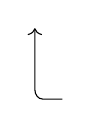
\begin{tikzpicture}[x=1cm,y=1cm]\draw[->] (0.35,0)--(0.1,0) to[out=180,in=270] (0,0.12)--(0,0.9);\end{tikzpicture}}}it is,  seems technically somewhat prohibitive,  at least in the present
set up (and with a distance of twenty years !).

\var{\over{35}{36}}{\hand{36}}{writing over}{ps_134-3_055-v0006}.  Now back to test categories,  and more specifically to her majesty
$\hand{\Delta}$ -  we still have to check it is a test category indeed !  The method \var{\inserted{suggested}}{\hand{suggested}}{insertion}{ps_134-3_055-v0007}
\margin{\diagram{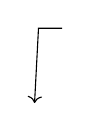
\begin{tikzpicture}[x=1cm,y=1cm]\draw[->] (0.35,0.95)--(0.05,0.95)--(0,0);\end{tikzpicture}}}last tuesday (p. 50) does work indeed,  without any reference to ``well-
known'' facts from the semi-simplicial theory.  To check  T H 1),  we take
of course $I = \hand{\Delta}_1$ and $e_o , e_1$ as usual,  we then have for every $n \hand{\in} \underline{N}$ to con-
struct a homotopy \var{\xout{\unsure{hx}}}{}{typewriter deletion}{ps_134-3_055-v0008}\var{\xout{\unsure{a}}}{}{typewriter deletion}{ps_134-3_055-v0009}
\[ h_n : \hand{\Delta}_n \, x \hand{\Delta}_1 \hand{\rightarrow} \hand{\Delta}_n \quad , \]
where the product and the arrow can be interpreted as one in (Cat) or even
in (Ord) of course  (of which $\hand{\Delta}$ is a full subcategory),  and there is a
unique such h if we take for $u_a$ the ``constant'' endomorphism of $\hand{\Delta}_n$ whose
\margin{*}value is the \uline{last} element of $\hand{\Delta}_n$ \hand{(41)}. There remains only (T H 2) - namely
\margin{ok if $\exists$ final object}to prove that the objects $\hand{\Delta}_n \, x \hand{\Delta}_1$ in $\hand{\Delta}^{\hand{\wedge}}$\var{\xout{xxx}}{}{typewriter deletion}{ps_134-3_055-v0010} are aspheric $(n \hand{\geq} 0)$.  F\var{\over{e}{o}}{\hand{o}}{writing over}{ps_134-3_055-v0011}r this
we cover \var{\inserted[typed]{$\hand{\Delta}'_n =$}}{$\hand{\Delta}'_n =$}{typed insertion}{ps_134-3_055-v0012} $\hand{\Delta}_n \, x \hand{\Delta}_1$ by maximal representable subobjects,  namely maximal flags
of the ordered product set\hand{(}  these are I guess what are called the ``shuff-
les'' in semi-simplicial algebra\hand{)}. It then turns out that $\hand{\Delta}'_n$ can be obtai-
ned by successive gluing of flags,  the intersection of each flag we add
with the sup or union of the preceding ones being just a subflag,  hence
representable and aspheric.  Thus we only have to make use of the \hand{``}Mayer-
Vietoris\hand{''} type easy lemma:
\uline{Lemma}  Let  U,V two subobjects of the final object \var{\inserted{e}}{\hand{e}}{insertion}{ps_134-3_055-v0013} of a topos \var{\inserted{[and covering e]}}{\hand{[and covering e]}}{insertion}{ps_134-3_055-v0014},  assume
U,V and U$\hand{\cap}$V aspheric,  then so is e\hand{,} i.e. so is the topos.

This finishes the proof of $\hand{\Delta}$ being a test category.  Of course,  one
cannot help thinking of the \var{\xout{acyclicity}}{}{typewriter deletion}{ps_134-3_055-v0015} \var{\inserted[typed]{apshericity}}{apshericity}{typed insertion}{ps_134-3_055-v0016} of \uline{all} the products $\hand{\Delta}_m \, x \hand{\Delta}_n$
as just meaning asphericity of the product ordered set (namely of the
corresponding category),  which follows for instance from the fact that it

%% END SOURCE ps_134-3_055
\ifnum\EditionMode=1
\psapparatusstart
\psentry{ps_134-3_055-v0001}{1}{typewriter overwriting}{\over[typed]{q}{a}}{a}{The superposed typed reading replaces the underlying reading.}
\psentry{ps_134-3_055-v0002}{2}{typewriter deletion}{\xout{s}}{}{The typewriter strikes out this material; it leaves the corrected running text.}
\psentry{ps_134-3_055-v0003}{3}{writing over}{\over{W}{W}}{\hand{W}}{The superposed handwritten reading replaces the underlying reading.}
\psentry{ps_134-3_055-v0004}{4}{writing over}{\over{n}{h}}{\hand{h}}{The superposed handwritten reading replaces the underlying reading.}
\psentry{ps_134-3_055-v0005}{5}{typed insertion}{\inserted[typed]{inverse}}{inverse}{The typed insertion is incorporated at its indicated position; insertion brackets leave the running text.}
\psentry{ps_134-3_055-v0006}{6}{writing over}{\over{35}{36}}{\hand{36}}{The superposed handwritten reading replaces the underlying reading.}
\psentry{ps_134-3_055-v0007}{7}{insertion}{\inserted{suggested}}{\hand{suggested}}{The handwritten insertion is incorporated at its indicated position; insertion brackets leave the running text.}
\psentry{ps_134-3_055-v0008}{8}{typewriter deletion}{\xout{\unsure{hx}}}{}{The typewriter strikes out this material; it leaves the corrected running text.}
\psentry{ps_134-3_055-v0009}{9}{typewriter deletion}{\xout{\unsure{a}}}{}{The typewriter strikes out this material; it leaves the corrected running text.}
\psentry{ps_134-3_055-v0010}{10}{typewriter deletion}{\xout{xxx}}{}{The typewriter strikes out this material; it leaves the corrected running text.}
\psentry{ps_134-3_055-v0011}{11}{writing over}{\over{e}{o}}{\hand{o}}{The superposed handwritten reading replaces the underlying reading.}
\psentry{ps_134-3_055-v0012}{12}{typed insertion}{\inserted[typed]{$\hand{\Delta}'_n =$}}{$\hand{\Delta}'_n =$}{The typed insertion is incorporated at its indicated position; insertion brackets leave the running text.}
\psentry{ps_134-3_055-v0013}{13}{insertion}{\inserted{e}}{\hand{e}}{The handwritten insertion is incorporated at its indicated position; insertion brackets leave the running text.}
\psentry{ps_134-3_055-v0014}{14}{insertion}{\inserted{[and covering e]}}{\hand{[and covering e]}}{The handwritten insertion is incorporated at its indicated position; insertion brackets leave the running text.}
\psentry{ps_134-3_055-v0015}{15}{typewriter deletion}{\xout{acyclicity}}{}{The typewriter strikes out this material; it leaves the corrected running text.}
\psentry{ps_134-3_055-v0016}{16}{typed insertion}{\inserted[typed]{apshericity}}{apshericity}{The typed insertion is incorporated at its indicated position; insertion brackets leave the running text.}
\psapparatusend
\fi
\pssource{ps_134-3_056}{134-3/56}{https://grothendieck.umontpellier.fr/web/viewer.html?file=../134-3.pdf\#page=57}
\psnumber{ps_134-3_056-v0001}{1}
\psnumber{ps_134-3_056-v0002}{2}
\psnumber{ps_134-3_056-v0003}{3}
\psnumber{ps_134-3_056-v0004}{4}
\psnumber{ps_134-3_056-v0005}{5}
\psnumber{ps_134-3_056-v0006}{6}
\psnumber{ps_134-3_056-v0007}{7}
\psnumber{ps_134-3_056-v0008}{8}
\psnumber{ps_134-3_056-v0009}{9}
\psnumber{ps_134-3_056-v0010}{10}
%% BEGIN SOURCE ps_134-3_056
% Pursuing Stacks (cotes 134-2 to 134-8): archive cote 134-3, site page 56 (PDF page 57), typescript page 56.
% typescript. Draft compared: ps2.tex:2830-2896.
% AI-transcribed by Claude Opus 5.5 (claude-opus-5-5, adaptive thinking, effort high), Message Batches API, batch ps1 (msgbatch_01Rv5hCaNTtUt4JHx1yqoHPL), 2026-11-12; image review recorded in records/CHECK_DECISIONS_134_3_4.tsv.
\scanpage{134-3/56}
\mspage{56}
has a final element.  But we should beware the vicious circle, as we
implicitly make the assumption that for an object C of (Cat)  (at least
an object C such as $\hand{\ensuremath{\Delta}}_{m}\mathrm{x}\hand{\ensuremath{\Delta}}_{n}$), if C is aspheric,  then so is the correspon-%
ding  \var{\xout{(C)x}}{}{typewriter deletion}{ps_134-3_056-v0001} element \hand{\ensuremath{\alpha}}(C) in $A^{\hand{\wedge}}$:
\[ \hand{\ensuremath{\alpha}}(C) : \var{\over{A}{\Delta}}{\hand{\Delta}}{writing over}{ps_134-3_056-v0002}_{n} \hand{\ensuremath{\longmapsto}} \mathrm{Hom}(\hand{\ensuremath{\Delta}}_{n},C) \quad , \]
namely the \uline{nerve} of C.  We expect of course something stronger to hold,
namely that for any C, \hand{\ensuremath{\alpha}}(C) has the same homotopy type as C  -  in fact
that we have a canonical isomorphism between the images of both in (Hot).
This relationship has still to be established,  as well as the similar
statement for \hand{\ensuremath{\beta}} : (Cat)\hand{\ensuremath{\to}}\var{\over{\unsure{\hand{\ensuremath{\widetilde{\Delta}}}}}{\ensuremath{\square}}}{\hand{\ensuremath{\square}}}{writing over}{ps_134-3_056-v0003}$^{\hand{\wedge}}$ , and accordingly with \hand{\ensuremath{\widetilde{\Delta}}} and \hand{\ensuremath{\widetilde{\square}}} .  For all
four categories (\var{\inserted{where}}{\hand{where}}{insertion}{ps_134-3_056-v0004} the simplicial cases are known to be test categories al-%
ready),  we have,  together with the category A (the would-be test category\hand{),}
a functor
\[ A \hand{\ensuremath{\longrightarrow}} (\mathrm{Cat}) \quad , \qquad \text{say} \quad a \hand{\ensuremath{\mapsto}} \hand{\ensuremath{\Delta}}_{a} \]
(notation inspired by the case A =\hand{\ensuremath{\Delta}}),  hence a functor
\[ (\mathrm{Cat}) \hand{\ensuremath{\xrightarrow{\ \alpha\ }}} A^{\hand{\wedge}} \quad , \quad \hand{\ensuremath{\alpha}}(C) = (a \hand{\ensuremath{\mapsto}} \mathrm{Hom}_{\mathrm{Cat}}(\hand{\ensuremath{\Delta}}_{a},C)) \quad , \]
and the question is to compare the homotopy types of C and \hand{\ensuremath{\alpha}}(C),  the lat-%
ter being defined of course as the homotopy type of $\var{\over[typed]{\unsure{A}}{A}}{A}{typewriter overwriting}{ps_134-3_056-v0005}_{/\hand{\ensuremath{\alpha}}(C)} \hand{\ensuremath{\simeq}} A_{/C}$ ,
the category of all pairs  (a,p) with a \hand{\ensuremath{\in}}Ob A and p: $\hand{\ensuremath{\Delta}}_{a}\hand{\ensuremath{\to}}$ C ,  arrows bet-%
ween pairs corresponding to \uline{strictly} commutative diagrams  in Cat
% Hand-drawn arrows are marked blue; typed objects remain plain.
\diagram{\begin{tikzcd}[row sep=small,column sep=small]
a' \ar[rr,color=blue,"\hand{\ensuremath{\Delta_u}}"] \ar[dr,color=blue,swap,"p'"] \& \& a \ar[dl,color=blue,"p"] \\
\& C \&
\end{tikzcd}}
.

\uline{Proposition}.  Let the data be as just said,  assume moreover that the cate-%
gories $\hand{\ensuremath{\Delta}}_{a}$ (a \hand{\ensuremath{\in}} Ob A) have final elements, \var{\inserted{that A is aspheric}}{\hand{that A is aspheric}}{insertion}{ps_134-3_056-v0006} and that \hand{\ensuremath{\alpha}}($\hand{\ensuremath{\Delta}}_{1}$) is aspheric
over the final element of $A^{\hand{\wedge}}$  (\var{\deleted{\unsure{which is}}}{}{deletion}{ps_134-3_056-v0007}\var{\inserted{the latter}}{\hand{the latter}}{insertion}{ps_134-3_056-v0008} automatic if A is a test category,
A\hand{\ensuremath{\longrightarrow}}(Cat) is fully faithful and $\hand{\ensuremath{\Delta}}_{1}$ belongs to it's essential image). Then
we can find for every C in (Cat) a \var{\xout{functor}}{}{typewriter deletion}{ps_134-3_056-v0009} "map" in (Cat) (i.e. a functor)
\margin{(*)} \[ \hand{\ensuremath{\varphi}} : A_{/C} \hand{\ensuremath{\to}} C \ , \]
functorial in C for variable C,  and this map being \var{\xout{a weak equivalencexxx}}{}{typewriter deletion}{ps_134-3_056-v0010}
aspheric,  and a fortiori a weak equivalence (hence induces an isomorphism
between the homotopy types).

This implies that the compositum  C\hand{\ensuremath{\mapsto}}$A_{/C}$  :
\[ (\mathrm{Cat}) \hand{\ensuremath{\xrightarrow{\ \alpha\ }}} A^{\hand{\wedge}} \hand{\ensuremath{\xrightarrow{\ \textcolor{black}{i}_{A}\ }}} (\mathrm{Cat}) \]
transforms weak equivalences into weak equivalences,  and that the functor
deduced from it by passage to the localized categories  $W^{-1}$(Cat) = (Hot)
is isomorphic to the identity functor of (Hot).

%% END SOURCE ps_134-3_056
\ifnum\EditionMode=1
\psapparatusstart
\psentry{ps_134-3_056-v0001}{1}{typewriter deletion}{\xout{(C)x}}{}{The typewriter strikes out this material; it leaves the corrected running text.}
\psentry{ps_134-3_056-v0002}{2}{writing over}{$\over{A}{\Delta}$}{$\hand{\Delta}$}{The superposed handwritten reading replaces the underlying reading.}
\psentry{ps_134-3_056-v0003}{3}{writing over}{\over{\unsure{\hand{\ensuremath{\widetilde{\Delta}}}}}{\ensuremath{\square}}}{\hand{\ensuremath{\square}}}{The superposed handwritten reading replaces the underlying reading.}
\psentry{ps_134-3_056-v0004}{4}{insertion}{\inserted{where}}{\hand{where}}{The handwritten insertion is incorporated at its indicated position; insertion brackets leave the running text.}
\psentry{ps_134-3_056-v0005}{5}{typewriter overwriting}{$\over[typed]{\unsure{A}}{A}$}{$A$}{The superposed typed reading replaces the underlying reading.}
\psentry{ps_134-3_056-v0006}{6}{insertion}{\inserted{that A is aspheric}}{\hand{that A is aspheric}}{The handwritten insertion is incorporated at its indicated position; insertion brackets leave the running text.}
\psentry{ps_134-3_056-v0007}{7}{deletion}{\deleted{\unsure{which is}}}{}{The author cancels this material by hand; it leaves the corrected running text.}
\psentry{ps_134-3_056-v0008}{8}{insertion}{\inserted{the latter}}{\hand{the latter}}{The handwritten insertion is incorporated at its indicated position; insertion brackets leave the running text.}
\psentry{ps_134-3_056-v0009}{9}{typewriter deletion}{\xout{functor}}{}{The typewriter strikes out this material; it leaves the corrected running text.}
\psentry{ps_134-3_056-v0010}{10}{typewriter deletion}{\xout{a weak equivalencexxx}}{}{The typewriter strikes out this material; it leaves the corrected running text.}
\psapparatusend
\fi
\pssource{ps_134-3_057}{134-3/57}{https://grothendieck.umontpellier.fr/web/viewer.html?file=../134-3.pdf\#page=58}
\psnumber{ps_134-3_057-v0001}{1}
\psnumber{ps_134-3_057-v0002}{2}
\psnumber{ps_134-3_057-v0003}{3}
\psnumber{ps_134-3_057-v0004}{4}
\psnumber{ps_134-3_057-v0005}{5}
\psnumber{ps_134-3_057-v0006}{6}
\psnumber{ps_134-3_057-v0007}{7}
\psnumber{ps_134-3_057-v0008}{8}
%% BEGIN SOURCE ps_134-3_057
% Pursuing Stacks (cotes 134-2 to 134-8): archive cote 134-3, site page 57 (PDF page 58), typescript page 57.
% typescript. Draft compared: ps2.tex:2879-2946.
% AI-transcribed by Claude Opus 5.5 (claude-opus-5-5, adaptive thinking, effort high), Message Batches API, batch ps1 (msgbatch_01Rv5hCaNTtUt4JHx1yqoHPL), 2026-11-12; image review recorded in records/CHECK_DECISIONS_134_3_4.tsv.
\scanpage{134-3/57}
\mspage{57}

To define a functor (*) , functorial in C for variable C, we only
have to choose a final element $e_a$ in each $\hand{\Delta}_a$ . For an element (a,p) of
$A_{/C}$ , we define
\[ \hand{\phi}(a,p) = p(e_a) \quad , \]
with evident extension to arrows of $A_{/C}$\hand{\unsure{,}}(NB here it is important that the
$e_a$ be \uline{final} elements of the $\hand{\Delta}_a$ , initial elements for a change would'nt
do at all !), thus we get the functor $\hand{\phi}$ , and functoriality with respect to
C is clear. Using the standart criterion of asphericity of a functor $\hand{\phi}$ ,
we have to check that the categories
\[ (A_{/C})_{/x} \]
for $x \hand{\in}$ Ob C are aspheric, but one checks at once that the category above
is canonically isomorphic to $A_{/C'}$ , where $C' = C_{/x}$ . Thus asphericity
of $\hand{\phi}$ for arbitrary C is equivalent to asphericity of $A_{/C}$ when C has a
final element, or equivalently, to asphericity of the element $\hand{\alpha}(C)$ \var{\over{o}{i}}{\hand{i}}{writing over}{ps_134-3_057-v0001}\var{\over{n}{n}}{\hand{n}}{writing over}{ps_134-3_057-v0002} $\hand{A}^{\hand{\wedge}}$
for such C. Now let $e_C$ be the final element of C, and consider the \var{\xout{stan}}{}{typewriter deletion}{ps_134-3_057-v0003}
unique homotopy
\[ h : \hand{\Delta}_1 x C \hand{\to} C \]
between $id_C$ and the constant functor from C to C with value $e_C$ . Applying
the functor $\hand{\alpha}$ we get a corresponding homotopy in $A^{\hand{\wedge}}$
\[ \var{\over{I}{I}}{\hand{I}}{writing over}{ps_134-3_057-v0004}\,\underset{\illegible{1}}{\var{\over{x}{x}}{\hand{x}}{writing over}{ps_134-3_057-v0005}}\,\hand{\alpha}(C) \hand{\to} \hand{\alpha}(C) \quad , \text{ where } I = \hand{\alpha}(\hand{\Delta}_1) \ , \]
between the identity map of $F = \hand{\alpha}(C)$ and a ``constant'' map $F \hand{\to} F$ . As we
assume that I is aspherical over the final element of $A^{\hand{\wedge}}$, hence $IxF \hand{\to} F$
is a weak equivalence, it follows that $F \hand{\to} e$ is a weak equivalence, hen-%
ce F is aspheric as e is supposed to be aspheric, which was to be proved.

If we apply this proposition to $A=\hand{\Delta}$ and $n \hand{\to} \hand{\Delta}_n$ , we are still
reduced to check just T H 2) (which we did above looking at shuffles),
whereas T H 1) appears superfluous now - we get asphericity of the
elements $\hand{\Delta}_m x \hand{\Delta}_n$ in $A^{\hand{\wedge}}$ as a consequence (but the homotopy argument used in \var{\inserted{the}}{\hand{the}}{insertion}{ps_134-3_057-v0006}
prop. is essentially the same as the one used for proving T H 1 ). This
proposition applies equally to the case when $A = \hand{\widetilde{\Delta}}$ (category of non ordered
simplices $\hand{\widetilde{\Delta}}_n$ ), here the natural functor
\[ \hand{i} : \hand{\widetilde{\Delta} \longrightarrow} \text{(Cat)} \quad , \hand{a \mapsto \mathfrak{P}^*}(a) \]
is obtained by associating to any finite set a the combinatorial simplex
it defines, embodied by the ordered set $\hand{\mathfrak{P}^*}(a)$ of it's facettes of all di-%
mensions, which can be identified \hand{with} the ordered set of all non-empty sub-%
sets of the finite set a. As we know already $\hand{\widetilde{\Delta}}$ is a test category, all
that remains to be done is to check in this case that $I = \hand{\alpha}(\hand{\Delta}_1)$ is asphe-%
ric (hence aspheric over the final object of $A^{\hand{\wedge}}$), Now this follows \var{\xout{from}}{}{typewriter deletion}{ps_134-3_057-v0007}
\var{\xout{the fact}}{}{typewriter deletion}{ps_134-3_057-v0008} again from a homotopy argument involving the unit segment substi-%

%% END SOURCE ps_134-3_057
\ifnum\EditionMode=1
\psapparatusstart
\psentry{ps_134-3_057-v0001}{1}{writing over}{\over{o}{i}}{\hand{i}}{The superposed handwritten reading replaces the underlying reading.}
\psentry{ps_134-3_057-v0002}{2}{writing over}{\over{n}{n}}{\hand{n}}{The superposed handwritten reading replaces the underlying reading.}
\psentry{ps_134-3_057-v0003}{3}{typewriter deletion}{\xout{stan}}{}{The typewriter strikes out this material; it leaves the corrected running text.}
\psentry{ps_134-3_057-v0004}{4}{writing over}{$\over{I}{I}$}{$\hand{I}$}{The superposed handwritten reading replaces the underlying reading.}
\psentry{ps_134-3_057-v0005}{5}{writing over}{$\over{x}{x}$}{$\hand{x}$}{The superposed handwritten reading replaces the underlying reading.}
\psentry{ps_134-3_057-v0006}{6}{insertion}{\inserted{the}}{\hand{the}}{The handwritten insertion is incorporated at its indicated position; insertion brackets leave the running text.}
\psentry{ps_134-3_057-v0007}{7}{typewriter deletion}{\xout{from}}{}{The typewriter strikes out this material; it leaves the corrected running text.}
\psentry{ps_134-3_057-v0008}{8}{typewriter deletion}{\xout{the fact}}{}{The typewriter strikes out this material; it leaves the corrected running text.}
\psapparatusend
\fi
\pssource{ps_134-3_058}{134-3/58}{https://grothendieck.umontpellier.fr/web/viewer.html?file=../134-3.pdf\#page=59}
\psnumber{ps_134-3_058-v0001}{1}
\psnumber{ps_134-3_058-v0002}{2}
\psnumber{ps_134-3_058-v0003}{3}
\psnumber{ps_134-3_058-v0004}{4}
\psnumber{ps_134-3_058-v0005}{5}
\psnumber{ps_134-3_058-v0006}{6}
\psnumber{ps_134-3_058-v0007}{7}
\psnumber{ps_134-3_058-v0008}{8}
\psnumber{ps_134-3_058-v0009}{9}
\psnumber{ps_134-3_058-v0010}{10}
\psnumber{ps_134-3_058-v0011}{11}
\psnumber{ps_134-3_058-v0012}{12}
\psnumber{ps_134-3_058-v0013}{13}
\psnumber{ps_134-3_058-v0014}{14}
\psnumber{ps_134-3_058-v0015}{15}
\psnumber{ps_134-3_058-v0016}{16}
\psnumber{ps_134-3_058-v0017}{17}
\psnumber{ps_134-3_058-v0018}{18}
\psnumber{ps_134-3_058-v0019}{19}
\psnumber{ps_134-3_058-v0020}{20}
\psnumber{ps_134-3_058-v0021}{21}
\psnumber{ps_134-3_058-v0022}{22}
\psnumber{ps_134-3_058-v0023}{23}
\psnumber{ps_134-3_058-v0024}{24}
\psnumber{ps_134-3_058-v0025}{25}
\psnumber{ps_134-3_058-v0026}{26}
\psnumber{ps_134-3_058-v0027}{27}
\psnumber{ps_134-3_058-v0028}{28}
%% BEGIN SOURCE ps_134-3_058
% Pursuing Stacks (cotes 134-2 to 134-8): archive cote 134-3, site page 58 (PDF page 59), typescript page 58.
% typescript. Draft compared: ps2.tex:2932-3005.
% AI-transcribed by Claude Opus 5.5 (claude-opus-5-5, adaptive thinking, effort high), Message Batches API, batch ps1 (msgbatch_01Rv5hCaNTtUt4JHx1yqoHPL), 2026-11-12; image review recorded in records/CHECK_DECISIONS_134_3_4.tsv.
\scanpage{134-3/58}
\mspage{58}

\margin{*} tute in $A^{\hand{\wedge}}$. We could formalize it as follows:\hand{..} \hand{(42).}

\margin{\unsure{cor. inst ci-dessous}} \var{\deleted{\uline{Corollary:} In the proposition above, the condition that $\hand{\alpha}(\hand{\Delta}_1)$ be aspheric}}{}{deletion}{ps_134-3_058-v0001}
\var{\deleted{over $e_{A^{\hand{\wedge}}}$ is a consequence of the following assumptions:}}{}{deletion}{ps_134-3_058-v0002}
\var{\deleted{a) The condition T 3 is valid in A , with the stronger assumption \xout{th}}}{}{deletion}{ps_134-3_058-v0003}
\var{\deleted{that I is aspheric over the final object e of $A^{\hand{\wedge}}$, and moreover :}}{}{deletion}{ps_134-3_058-v0004}
\var{\deleted{b) for every $a \hand{\in} \mathrm{Ob}\, A$ and $u : a \hand{\longrightarrow} I$, let $a_u = u^{-1}(e_o)$ (subobject}}{}{deletion}{ps_134-3_058-v0005}
\var{\deleted{of a in $A^{\hand{\wedge}}$), $\hand{\Delta}_{a_u} = \underset{b \text{ in } A_{/a_u}}{\underset{\hand{\longrightarrow}}{\mathrm{lim}}} \hand{\Delta}_b$ , and $\hand{\Delta}_{a,u} = \mathrm{Im}\,(\hand{\Delta}_{a_u} \hand{\to} \hand{\Delta}_a)$.}}{}{deletion}{ps_134-3_058-v0006}

\var{\deleted{We assume that Ob $\hand{\Delta}_{a,u}$ is a \uline{crible} in $\hand{\Delta}_a$ , say $C_u$ .}}{}{deletion}{ps_134-3_058-v0007}

\var{\deleted{Indeed, interpreting $\hand{\alpha}(\hand{\Delta}_1)$ as the functor $a \hand{\mapsto} \mathrm{Crib}\, \hand{\Delta}_a$ , we}}{}{deletion}{ps_134-3_058-v0008}
\var{\deleted{define a homotopy}}{}{deletion}{ps_134-3_058-v0009}
\var{\deleted{\[ h : I\mathrm{x}F\deleted{\unsure{(\hand{\alpha}(\hand{\Delta}_1))}} \hand{\to} F \deleted{\unsure{\hand{\alpha}(\hand{\Delta}_1)}} \quad \text{(where } F = \hand{\alpha}(\hand{\Delta}_1)\text{ )} \]}}{}{deletion}{ps_134-3_058-v0010}
\var{\deleted{from the identity $\mathrm{id}_F$ to the constant map $c : F \hand{\to} F$ associating to every}}{}{deletion}{ps_134-3_058-v0011}
\var{\deleted{crible in some $\hand{\Delta}_a$ the empty crible in the same, by taking for every a}}{}{deletion}{ps_134-3_058-v0012}
\var{\deleted{in A the map}}{}{deletion}{ps_134-3_058-v0013}
\var{\deleted{\[ (u, C_o) \hand{\longmapsto} C_u \hand{\cap} C_o \quad . \]}}{}{deletion}{ps_134-3_058-v0014}
\var{\deleted{It follows that $F \hand{\longmapsto} e$ is a weak equivalence, and the same argument in}}{}{deletion}{ps_134-3_058-v0015}
\var{\deleted{any induced category $A_{/a}$ shows that this is universally so i.e. $F \hand{\to} e$ is}}{}{deletion}{ps_134-3_058-v0016}
\var{\deleted{aspheric , O.K.}}{}{deletion}{ps_134-3_058-v0017}

\var{\deleted{In the case \inserted[typed]{above} $A = \hand{\tilde{\Delta}}$, we get indeed that for $u : a \hand{\to} I$, $a_u$ is \inserted{empty or} in A}}{}{deletion}{ps_134-3_058-v0018}
\var{\deleted{and $\hand{\Delta}_{a_u} \hand{\to} \hand{\Delta}_a$ is a full embedding, turning $\hand{\Delta}_{a_u}$ into a crible in $\hand{\Delta}_a$ ,}}{}{deletion}{ps_134-3_058-v0019}
\var{\deleted{thus \xout{a) and} b) is satisfied (with the usual choice $I = \hand{\tilde{\Delta}}_1$ of course).}}{}{deletion}{ps_134-3_058-v0020}

21.3.

37. By the end of the notes two days ago, there was the pretty strong
impression of repeating the same argument all over again, in very similar
situations. When I tried to pin down this feeling, first thing that oc-%
cured to me was that the \var{\inserted{homotopy}}{\hand{homotopy}}{insertion}{ps_134-3_058-v0021} equivalence I was after $A_{/C} \hand{\longrightarrow} C$ (in the propo-%
sition of \var{\over{p}{\S}}{\hand{\S}}{writing over}{ps_134-3_058-v0022}.\var{\over{5}{3}}{\hand{3}}{writing over}{ps_134-3_058-v0023}6), when concerned with a\var{\xout{n}}{}{typewriter deletion}{ps_134-3_058-v0024} general functor $A \hand{\longrightarrow} (\mathrm{Cat})$,
and the criterion obtained, was applicable to the situation I was concer-%
ned with at the very start when defining test categories, namely when
looking at the \uline{canonical} functor $A \hand{\longrightarrow} (\mathrm{Cat})$ given by $a \hand{\longmapsto} A_{/a}$ ; and \var{\inserted{that this}}{\hand{that this}}{insertion}{ps_134-3_058-v0025} gave
a criterion in this case for A to be a test-category in the wider sense,
which I had overlooked when peeling out the caracterisation of test cate-%
gories (cf. theorem of p. 46). Finally it bec\var{\over{o}{a}}{\hand{a}}{writing over}{ps_134-3_058-v0026}mes clear that it \var{\over{was}{is}}{\hand{is}}{writing over}{ps_134-3_058-v0027} about
% NOTE: the right edge of the next line is cut; the typed word ends "repet" at the edge
time to recast from scratch the asphericity story, and (by one more repet%
tition) tell it anew in a way stripped from it's repetitive features\var{\over{.}{!}}{\hand{!}}{writing over}{ps_134-3_058-v0028}

%% END SOURCE ps_134-3_058
\ifnum\EditionMode=1
\psapparatusstart
\psentry{ps_134-3_058-v0001}{1}{deletion}{\deleted{\uline{Corollary:} In the proposition above, the condition that $\hand{\alpha}(\hand{\Delta}_1)$ be aspheric}}{}{The author cancels this material by hand; it leaves the corrected running text.}
\psentry{ps_134-3_058-v0002}{2}{deletion}{\deleted{over $e_{A^{\hand{\wedge}}}$ is a consequence of the following assumptions:}}{}{The author cancels this material by hand; it leaves the corrected running text.}
\psentry{ps_134-3_058-v0003}{3}{deletion}{\deleted{a) The condition T 3 is valid in A , with the stronger assumption \xout{th}}}{}{The author cancels this material by hand; it leaves the corrected running text.}
\psentry{ps_134-3_058-v0004}{4}{deletion}{\deleted{that I is aspheric over the final object e of $A^{\hand{\wedge}}$, and moreover :}}{}{The author cancels this material by hand; it leaves the corrected running text.}
\psentry{ps_134-3_058-v0005}{5}{deletion}{\deleted{b) for every $a \hand{\in} \mathrm{Ob}\, A$ and $u : a \hand{\longrightarrow} I$, let $a_u = u^{-1}(e_o)$ (subobject}}{}{The author cancels this material by hand; it leaves the corrected running text.}
\psentry{ps_134-3_058-v0006}{6}{deletion}{\deleted{of a in $A^{\hand{\wedge}}$), $\hand{\Delta}_{a_u} = \underset{b \text{ in } A_{/a_u}}{\underset{\hand{\longrightarrow}}{\mathrm{lim}}} \hand{\Delta}_b$ , and $\hand{\Delta}_{a,u} = \mathrm{Im}\,(\hand{\Delta}_{a_u} \hand{\to} \hand{\Delta}_a)$.}}{}{The author cancels this material by hand; it leaves the corrected running text.}
\psentry{ps_134-3_058-v0007}{7}{deletion}{\deleted{We assume that Ob $\hand{\Delta}_{a,u}$ is a \uline{crible} in $\hand{\Delta}_a$ , say $C_u$ .}}{}{The author cancels this material by hand; it leaves the corrected running text.}
\psentry{ps_134-3_058-v0008}{8}{deletion}{\deleted{Indeed, interpreting $\hand{\alpha}(\hand{\Delta}_1)$ as the functor $a \hand{\mapsto} \mathrm{Crib}\, \hand{\Delta}_a$ , we}}{}{The author cancels this material by hand; it leaves the corrected running text.}
\psentry{ps_134-3_058-v0009}{9}{deletion}{\deleted{define a homotopy}}{}{The author cancels this material by hand; it leaves the corrected running text.}
\psentry{ps_134-3_058-v0010}{10}{deletion}{\deleted{\[ h : I\mathrm{x}F\deleted{\unsure{(\hand{\alpha}(\hand{\Delta}_1))}} \hand{\to} F \deleted{\unsure{\hand{\alpha}(\hand{\Delta}_1)}} \quad \text{(where } F = \hand{\alpha}(\hand{\Delta}_1)\text{ )} \]}}{}{The author cancels this material by hand; it leaves the corrected running text.}
\psentry{ps_134-3_058-v0011}{11}{deletion}{\deleted{from the identity $\mathrm{id}_F$ to the constant map $c : F \hand{\to} F$ associating to every}}{}{The author cancels this material by hand; it leaves the corrected running text.}
\psentry{ps_134-3_058-v0012}{12}{deletion}{\deleted{crible in some $\hand{\Delta}_a$ the empty crible in the same, by taking for every a}}{}{The author cancels this material by hand; it leaves the corrected running text.}
\psentry{ps_134-3_058-v0013}{13}{deletion}{\deleted{in A the map}}{}{The author cancels this material by hand; it leaves the corrected running text.}
\psentry{ps_134-3_058-v0014}{14}{deletion}{\deleted{\[ (u, C_o) \hand{\longmapsto} C_u \hand{\cap} C_o \quad . \]}}{}{The author cancels this material by hand; it leaves the corrected running text.}
\psentry{ps_134-3_058-v0015}{15}{deletion}{\deleted{It follows that $F \hand{\longmapsto} e$ is a weak equivalence, and the same argument in}}{}{The author cancels this material by hand; it leaves the corrected running text.}
\psentry{ps_134-3_058-v0016}{16}{deletion}{\deleted{any induced category $A_{/a}$ shows that this is universally so i.e. $F \hand{\to} e$ is}}{}{The author cancels this material by hand; it leaves the corrected running text.}
\psentry{ps_134-3_058-v0017}{17}{deletion}{\deleted{aspheric , O.K.}}{}{The author cancels this material by hand; it leaves the corrected running text.}
\psentry{ps_134-3_058-v0018}{18}{deletion}{\deleted{In the case \inserted[typed]{above} $A = \hand{\tilde{\Delta}}$, we get indeed that for $u : a \hand{\to} I$, $a_u$ is \inserted{empty or} in A}}{}{The author cancels this material by hand; it leaves the corrected running text.}
\psentry{ps_134-3_058-v0019}{19}{deletion}{\deleted{and $\hand{\Delta}_{a_u} \hand{\to} \hand{\Delta}_a$ is a full embedding, turning $\hand{\Delta}_{a_u}$ into a crible in $\hand{\Delta}_a$ ,}}{}{The author cancels this material by hand; it leaves the corrected running text.}
\psentry{ps_134-3_058-v0020}{20}{deletion}{\deleted{thus \xout{a) and} b) is satisfied (with the usual choice $I = \hand{\tilde{\Delta}}_1$ of course).}}{}{The author cancels this material by hand; it leaves the corrected running text.}
\psentry{ps_134-3_058-v0021}{21}{insertion}{\inserted{homotopy}}{\hand{homotopy}}{The handwritten insertion is incorporated at its indicated position; insertion brackets leave the running text.}
\psentry{ps_134-3_058-v0022}{22}{writing over}{\over{p}{\S}}{\hand{\S}}{The superposed handwritten reading replaces the underlying reading.}
\psentry{ps_134-3_058-v0023}{23}{writing over}{\over{5}{3}}{\hand{3}}{The superposed handwritten reading replaces the underlying reading.}
\psentry{ps_134-3_058-v0024}{24}{typewriter deletion}{\xout{n}}{}{The typewriter strikes out this material; it leaves the corrected running text.}
\psentry{ps_134-3_058-v0025}{25}{insertion}{\inserted{that this}}{\hand{that this}}{The handwritten insertion is incorporated at its indicated position; insertion brackets leave the running text.}
\psentry{ps_134-3_058-v0026}{26}{writing over}{\over{o}{a}}{\hand{a}}{The superposed handwritten reading replaces the underlying reading.}
\psentry{ps_134-3_058-v0027}{27}{writing over}{\over{was}{is}}{\hand{is}}{The superposed handwritten reading replaces the underlying reading.}
\psentry{ps_134-3_058-v0028}{28}{writing over}{\over{.}{!}}{\hand{!}}{The superposed handwritten reading replaces the underlying reading.}
\psapparatusend
\fi
\pssource{ps_134-3_059}{134-3/59}{https://grothendieck.umontpellier.fr/web/viewer.html?file=../134-3.pdf\#page=60}
\psnumber{ps_134-3_059-v0001}{1}
\psnumber{ps_134-3_059-v0002}{2}
\psnumber{ps_134-3_059-v0003}{3}
\psnumber{ps_134-3_059-v0004}{4}
\psnumber{ps_134-3_059-v0005}{5}
\psnumber{ps_134-3_059-v0006}{6}
\psnumber{ps_134-3_059-v0007}{7}
\psnumber{ps_134-3_059-v0008}{8}
\psnumber{ps_134-3_059-v0009}{9}
\psnumber{ps_134-3_059-v0010}{10}
\psnumber{ps_134-3_059-v0011}{11}
\psnumber{ps_134-3_059-v0012}{12}
\psnumber{ps_134-3_059-v0013}{13}
%% BEGIN SOURCE ps_134-3_059
% Pursuing Stacks (cotes 134-2 to 134-8): archive cote 134-3, site page 59 (PDF page 60), typescript page 59.
% typescript. Draft compared: ps2.tex:2991-3069.
% AI-transcribed by Claude Opus 5.5 (claude-opus-5-5, adaptive thinking, effort high), Message Batches API, batch ps1 (msgbatch_01Rv5hCaNTtUt4JHx1yqoHPL), 2026-11-12; image review recorded in records/CHECK_DECISIONS_134_3_4.tsv.
\scanpage{134-3/59}
\mspage{59}

On a more technical level,  I got aware too that the last corollary
\margin{\diagram{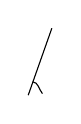
\begin{tikzpicture}[x=1cm,y=1cm]\draw (0.3,0.85)--(0,0);\draw (0.055,0.17) to[out=-5,in=130] (0.18,0.02);\end{tikzpicture}} $(^{42})$} stated was slightly uncorrect,  because it is by no means clear that the
crible \var{\inserted{$C_u$}}{\hand{$C_u$}}{insertion}{ps_134-3_059-v0001} constructed there is  functorial in u  i.e. corresponds to a map
I\hand{\ensuremath{\to\alpha}}(\hand{\ensuremath{\Delta}}$_1$) ,  this in fact has still to be assum\var{\xout{m}}{}{typewriter deletion}{ps_134-3_059-v0002}ed  (and turns out to be
\var{\xout{automatic}}{}{typewriter deletion}{ps_134-3_059-v0003} satisfied in all cases which turned up naturally so far and which
I looked up).  But let's now \hand{``}retell the story\hand{''}!

One key notion visibly in the homotopy technique used,  and which
needs a name in the long last,  is the notion of a \uline{homotopy} \uline{interval}\var{\xout{\unsure{,}}}{}{typewriter deletion}{ps_134-3_059-v0004}
( "segment homotopique" in French).  To be really outspoken about the very
formal nature of this notion and the way it will be used,  let's develop
it in any category \hand{\ensuremath{\mathcal{A}}} endowed with a subset  W \hand{\ensuremath{\subset}} Fl(\hand{\ensuremath{\mathcal{A}}}) of the set of
arrows of \hand{\ensuremath{\mathcal{A}}} , and satisfying the usual conditions :

a)  W contains all isomorphisms of \hand{\ensuremath{\mathcal{A}}} ,

b)  for two composable arrows u,v in \hand{\ensuremath{\mathcal{A}}},  if  two among u,v, vu are
in W,  so is the third,  and

c)  if  i: $F_o$ \hand{\ensuremath{\to}} F,and r: F \hand{\ensuremath{\to}} $F_o$ is a left inverse(i.e. a retraction ),
and if \var{\xout{ir}}{}{typewriter deletion}{ps_134-3_059-v0005} p = ir : F \hand{\ensuremath{\to}} F is in W,  so is r (and hence i too).

The condition c) \var{\inserted[typed]{here}}{here}{typed insertion}{ps_134-3_059-v0006} is the ingredient slightly stronger than what we used
to call "mild saturation property" of W,  meaning a) and b).

We'll call \uline{homotopy} \uline{\var{\over[typed]{seg}{int}}{int}{typewriter overwriting}{ps_134-3_059-v0007}erval} \uline{in} \hand{\ensuremath{\mathcal{A}}} (with respect to the notion of
"weak equivalence" W,  which will generally be implicit and specified by
context)  a triple (I,$e_o$,$e_1$) ,  where I is an object of \hand{\ensuremath{\mathcal{A}}} , $e_o$ and $e_1$
\margin{* provisional \uline{separating} W-homotopy interval} two subobjects,  such that the following conditions a) to c) hold \hand{\ensuremath{(^{43})}}

a)  $e_o$ and $e_1$ are \var{\xout{unit}}{}{typewriter deletion}{ps_134-3_059-v0008} final objects of \hand{\ensuremath{\mathcal{A}}} ,
which implies that \hand{\ensuremath{\mathcal{A}}} has a final object, unique up to unique isomorphism,
which we'll debote by e$_{\hand{\ensuremath{\mathcal{A}}}}$ or simply e , so that the data  $e_o$,$e_1$ in I are
equivalent to giving two sections
\[ \hand{\ensuremath{\delta}}_o , \hand{\ensuremath{\delta}}_1 :\ e \hand{\ensuremath{\to}} I \]
of I over e.  Note that  $e_o$\hand{\ensuremath{\cap}}$e_1$ \hand{\ensuremath{=}} Ker(\hand{\ensuremath{\delta}}$_o$,\hand{\ensuremath{\delta}}$_1$).

b)  $e_o$\hand{\ensuremath{\cap}}$e_1$ = \hand{\ensuremath{\emptyset_{\mathcal{A}}}} (a strict initial element of \hand{\ensuremath{\mathcal{A}}} ) ,

c)  I \hand{\ensuremath{\to}} e is "universally in W" or,  as we'll say, is W-\uline{aspheric} or
simply aspheric ,

which just means here that \var{\inserted{I $\to$ e is "squarable" and that}}{\hand{I $\to$ e is "squarable" and that}}{insertion}{ps_134-3_059-v0009} for any  F in Ob \hand{\ensuremath{\mathcal{A}}} ,  FxI \hand{\ensuremath{\to}} F is in W i.e.
is a "weak equivalence".

It is clear that if (I,$e_o$,$e_1$) is a homotopy \var{\xout{segment}}{}{typewriter deletion}{ps_134-3_059-v0010}\var{\inserted[typed]{interval}}{interval}{typed insertion}{ps_134-3_059-v0011} in \hand{\ensuremath{\mathcal{A}}}, then
for any F \hand{\ensuremath{\in}} Ob \hand{\ensuremath{\mathcal{A}}} ,  the"induced \var{\xout{segment}}{}{typewriter deletion}{ps_134-3_059-v0012}\var{\inserted[typed]{interval}}{interval}{typed insertion}{ps_134-3_059-v0013}"in \hand{\ensuremath{\mathcal{A}}}$_{/F}$ ,  namely (IxF,$e_o$xF,$e_1$xF)
is a homotopy interval in \hand{\ensuremath{\mathcal{A}}}$_{/F}$ .

%% END SOURCE ps_134-3_059
\ifnum\EditionMode=1
\psapparatusstart
\psentry{ps_134-3_059-v0001}{1}{insertion}{\inserted{$C_u$}}{\hand{$C_u$}}{The handwritten insertion is incorporated at its indicated position; insertion brackets leave the running text.}
\psentry{ps_134-3_059-v0002}{2}{typewriter deletion}{\xout{m}}{}{The typewriter strikes out this material; it leaves the corrected running text.}
\psentry{ps_134-3_059-v0003}{3}{typewriter deletion}{\xout{automatic}}{}{The typewriter strikes out this material; it leaves the corrected running text.}
\psentry{ps_134-3_059-v0004}{4}{typewriter deletion}{\xout{\unsure{,}}}{}{The typewriter strikes out this material; it leaves the corrected running text.}
\psentry{ps_134-3_059-v0005}{5}{typewriter deletion}{\xout{ir}}{}{The typewriter strikes out this material; it leaves the corrected running text.}
\psentry{ps_134-3_059-v0006}{6}{typed insertion}{\inserted[typed]{here}}{here}{The typed insertion is incorporated at its indicated position; insertion brackets leave the running text.}
\psentry{ps_134-3_059-v0007}{7}{typewriter overwriting}{\over[typed]{seg}{int}}{int}{The superposed typed reading replaces the underlying reading.}
\psentry{ps_134-3_059-v0008}{8}{typewriter deletion}{\xout{unit}}{}{The typewriter strikes out this material; it leaves the corrected running text.}
\psentry{ps_134-3_059-v0009}{9}{insertion}{\inserted{I $\to$ e is "squarable" and that}}{\hand{I $\to$ e is "squarable" and that}}{The handwritten insertion is incorporated at its indicated position; insertion brackets leave the running text.}
\psentry{ps_134-3_059-v0010}{10}{typewriter deletion}{\xout{segment}}{}{The typewriter strikes out this material; it leaves the corrected running text.}
\psentry{ps_134-3_059-v0011}{11}{typed insertion}{\inserted[typed]{interval}}{interval}{The typed insertion is incorporated at its indicated position; insertion brackets leave the running text.}
\psentry{ps_134-3_059-v0012}{12}{typewriter deletion}{\xout{segment}}{}{The typewriter strikes out this material; it leaves the corrected running text.}
\psentry{ps_134-3_059-v0013}{13}{typed insertion}{\inserted[typed]{interval}}{interval}{The typed insertion is incorporated at its indicated position; insertion brackets leave the running text.}
\psapparatusend
\fi
\pssource{ps_134-3_060}{134-3/60}{https://grothendieck.umontpellier.fr/web/viewer.html?file=../134-3.pdf\#page=61}
\psnumber{ps_134-3_060-v0001}{1}
\psnumber{ps_134-3_060-v0002}{2}
\psnumber{ps_134-3_060-v0003}{3}
\psnumber{ps_134-3_060-v0004}{4}
\psnumber{ps_134-3_060-v0005}{5}
\psnumber{ps_134-3_060-v0006}{6}
\psnumber{ps_134-3_060-v0007}{7}
\psnumber{ps_134-3_060-v0008}{8}
\psnumber{ps_134-3_060-v0009}{9}
\psnumber{ps_134-3_060-v0010}{10}
\psnumber{ps_134-3_060-v0011}{11}
\psnumber{ps_134-3_060-v0012}{12}
\psnumber{ps_134-3_060-v0013}{13}
\psnumber{ps_134-3_060-v0014}{14}
\psnumber{ps_134-3_060-v0015}{15}
\psnumber{ps_134-3_060-v0016}{16}
\psnumber{ps_134-3_060-v0017}{17}
\psnumber{ps_134-3_060-v0018}{18}
\psnumber{ps_134-3_060-v0019}{19}
\psnumber{ps_134-3_060-v0020}{20}
\psnumber{ps_134-3_060-v0021}{21}
\psnumber{ps_134-3_060-v0022}{22}
\psnumber{ps_134-3_060-v0023}{23}
\psnumber{ps_134-3_060-v0024}{24}
\psnumber{ps_134-3_060-v0025}{25}
\psnumber{ps_134-3_060-v0026}{26}
\psnumber{ps_134-3_060-v0027}{27}
\psnumber{ps_134-3_060-v0028}{28}
\psnumber{ps_134-3_060-v0029}{29}
%% BEGIN SOURCE ps_134-3_060
% Pursuing Stacks (cotes 134-2 to 134-8): archive cote 134-3, site page 60 (PDF page 61), typescript page 60.
% typescript. Draft compared: ps2.tex:3049-3123.
% AI-transcribed by Claude Opus 5.5 (claude-opus-5-5, adaptive thinking, effort high), Message Batches API, batch ps1 (msgbatch_01Rv5hCaNTtUt4JHx1yqoHPL), 2026-11-12; image review recorded in records/CHECK_DECISIONS_134_3_4.tsv.
\scanpage{134-3/60}
\mspage{\hand{60}}

We now get the (essentially trivial)
\uline{Homotopy lemma} \ Let \ $h\colon FxI \hand{\longrightarrow} F$ be a ``homotopy'' with respect to $(I,e_o,e_1)$
of $\mathrm{id}_F$ \ with a constant map \var{\xout{ix}}{}{typewriter deletion}{ps_134-3_060-v0001} $c = ir\colon F \hand{\to} F$ , \ where $r\colon F \hand{\longrightarrow} e$ and \var{\xout{i}}{}{typewriter deletion}{ps_134-3_060-v0002}
$i\colon e \hand{\to} F$ is a section of $F$ over $e$. \ Then $F \hand{\to} e$ is \ W-aspheric.

In the proof of this lemma, \ we make use of a)b)c) for W, \ but only
of a)c) for $(I,e_o,e_1)$ \ namely we don't even need \ $e_o \hand{\cap} e_1 = \hand{\emptyset}_{\hand{\mathcal{A}}}$ . \ This is
\var{\inserted[typed]{still the case for}}{still the case for}{typed insertion}{ps_134-3_060-v0003} \var{\xout{property however will be used in}}{}{typewriter deletion}{ps_134-3_060-v0004} the proof of the
\uline{Comparison lemma for homotopy intervals}: \ Let L be an object of \hand{\ensuremath{\mathcal{A}}} , squa-%
rable over e and endowed with a composition law \ $x\hand{\wedge}y$ ; \ let \ $\var{\over{e}{\delta}}{\hand{\delta}}{writing over}{ps_134-3_060-v0005}_i^L \colon e \hand{\to} L$
be two sections of L (i \hand{\ensuremath{\in\{}}0,1\hand{\ensuremath{\}}} ), \ which are respectively a left unit and a
zero element for the multiplication,namely the corresponding elements
$\hand{e}_o^{\var{\over[typed]{\illegible{1}}{a}}{a}{typewriter overwriting}{ps_134-3_060-v0006}},\hand{e}_1^{\var{\over[typed]{\illegible{1}}{a}}{a}{typewriter overwriting}{ps_134-3_060-v0007}}$ \ in any Hom(\var{\over[typed]{\illegible{1}}{a}}{a}{typewriter overwriting}{ps_134-3_060-v0008},L) satisfy
\[ \hand{e}_{\var{\over{\unsure{o}}{1}}{\hand{1}}{writing over}{ps_134-3_060-v0009}}^{\var{\over[typed]{\illegible{1}}{a}}{a}{typewriter overwriting}{ps_134-3_060-v0010}} \hand{\wedge} x = x \ , \ \hand{e}_{\var{\over{\unsure{1}}{0}}{\hand{0}}{writing over}{ps_134-3_060-v0011}}^{\var{\over[typed]{\illegible{1}}{a}}{a}{typewriter overwriting}{ps_134-3_060-v0012}} \hand{\wedge} x \ = \hand{e}_{\var{\over{\unsure{1}}{0}}{\hand{0}}{writing over}{ps_134-3_060-v0013}}^{\var{\over[typed]{\illegible{1}}{a}}{a}{typewriter overwriting}{ps_134-3_060-v0014}} \]
for any x in Hom(\var{\over[typed]{\illegible{1}}{a}}{a}{typewriter overwriting}{ps_134-3_060-v0015},L). \ Assume moreover we got a homotopy interval $(I,e_o,$
$e_1)$ and a \hand{``}map of intervals\hand{''}
\[ \hand{\phi}\colon I \hand{\longrightarrow} L \]
(in the sense: \ compatible with endpoints). \ Then \ $\mathrm{id}_L$ is homotopic(with
respect to $(I,e_o,e_1)$) to the constant map $c_{\hand{\unsure{0|a}}}\colon L \hand{\to} L$ defined by $\hand{\delta}^L_{\hand{\unsure{0|a}}}$ , \ and
hence by the previous homotopy lemma, \ $L \hand{\to} e$ is W-aspheric and therefore
\var{\xout{\illegible{1}}}{}{typewriter deletion}{ps_134-3_060-v0016} L endowed with \ $e_o^L ,e_1^L$ \ defined by $\hand{\delta}_o^L,\hand{\delta}_1^L$ \ is itself a homotopy inter-%
val in \hand{\ensuremath{\mathcal{A}}} (provided, \ at least, we know \ that \ $e_o^L \hand{\cap} e_1^L = \hand{\emptyset}$ ).

The homotopy h is simply given \ (for \ $u\colon \var{\over[typed]{\illegible{1}}{a}}{a}{typewriter overwriting}{ps_134-3_060-v0017} \hand{\to} \var{\over[typed]{\illegible{1}}{I}}{I}{typewriter overwriting}{ps_134-3_060-v0018}$, \ $x\colon \var{\over[typed]{\illegible{1}}{a}}{a}{typewriter overwriting}{ps_134-3_060-v0019} \hand{\to} L$) by
\[ h(\var{\over[typed]{\illegible{1}}{x}}{x}{typewriter overwriting}{ps_134-3_060-v0020},\var{\over[typed]{\illegible{1}}{u}}{u}{typewriter overwriting}{ps_134-3_060-v0021}) = \var{\xout{uxxxxx}}{}{typewriter deletion}{ps_134-3_060-v0022} \ \hand{\phi}(u) \hand{\wedge} x \ , \]
when a factors through $e_{\hand{1}}$ then $\hand{\phi}(u) = \hand{e}^a_{\hand{1}}$ \ and hence \ $h(x,u)=x$, \ if it
factors through $e_{\hand{0}}$ then $\hand{\phi}(u) = \hand{e}^a_{\hand{0}}$ \ and we get $h(x,u) = \hand{e}^a_{\hand{0}}$ , \ qed.
\uline{Corollary} \ Assume in \hand{\ensuremath{\mathcal{A}}} (endowed with W) finite inverse limits exist
(i.e. final object and fibered products exist), \ and moreover that the
\var{\deleted{functor}}{}{deletion}{ps_134-3_060-v0023}\var{\inserted{presheaf}}{\hand{presheaf}}{insertion}{ps_134-3_060-v0024} \hand{on $\mathcal{A}$}
\[ F \hand{\longmapsto} \text{set ob all subobjects of } F \]
is representable by an element L of \hand{\ensuremath{\mathcal{A}}} (the ``Lawvere element''). \ \var{\xout{Then}}{}{typewriter deletion}{ps_134-3_060-v0025}
Assume moreover \hand{\ensuremath{\mathcal{A}}} has a\var{\xout{n}}{}{typewriter deletion}{ps_134-3_060-v0026} strict initia\var{\over[typed]{\unsure{b}}{l}}{l}{typewriter overwriting}{ps_134-3_060-v0027} element $\hand{\emptyset}_{\hand{\mathcal{A}}}$, i.e. an initial
element and that \var{\deleted{\xout{for}}}{}{deletion}{ps_134-3_060-v0028} any \ map \ $\underset{\text{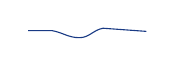
\begin{tikzpicture}[x=1cm,y=1cm,baseline]\draw[color=blue] (0,0.05)--(0.3,0.05) to[out=-10,in=180] (0.65,-0.04) to[out=0,in=190] (0.95,0.08)--(1.5,0.04);\end{tikzpicture}}}{a \hand{\to} \hand{\emptyset}_{\hand{\mathcal{A}}}}$ \ is an isomorphism. \ Consider the
two sections of L over e , $\hand{\delta}^L_{\hand{1}}$ \ and \ $\hand{\delta}^L_{\hand{0}}$ , \ corresponding to the full and
to the empty subobject of e, \ so that we get visibly \ $e_o^L \hand{\cap} e_1^L = \hand{\emptyset}$ \ .
\var{\over{t}{T}}{\hand{T}}{writing over}{ps_134-3_060-v0029}hen, \ for a homotopy interval to exist in \hand{\ensuremath{\mathcal{A}}} , it is necessay and suf-%
ficient that L be W-aspheric over e , \ i.e. that $(L,e_o^L ,e_1^L )$ \ be a homoto-%
py interval.

By the comparison lemma, \ it is enough to show that for any homotopy
\unsure{interval} \ $(I,e_o,e_1)$ \ in \hand{\ensuremath{\mathcal{A}}}, \ there exists a morphism of ``intervals''

%% END SOURCE ps_134-3_060
\ifnum\EditionMode=1
\psapparatusstart
\psentry{ps_134-3_060-v0001}{1}{typewriter deletion}{\xout{ix}}{}{The typewriter strikes out this material; it leaves the corrected running text.}
\psentry{ps_134-3_060-v0002}{2}{typewriter deletion}{\xout{i}}{}{The typewriter strikes out this material; it leaves the corrected running text.}
\psentry{ps_134-3_060-v0003}{3}{typed insertion}{\inserted[typed]{still the case for}}{still the case for}{The typed insertion is incorporated at its indicated position; insertion brackets leave the running text.}
\psentry{ps_134-3_060-v0004}{4}{typewriter deletion}{\xout{property however will be used in}}{}{The typewriter strikes out this material; it leaves the corrected running text.}
\psentry{ps_134-3_060-v0005}{5}{writing over}{$\over{e}{\delta}$}{$\hand{\delta}$}{The superposed handwritten reading replaces the underlying reading.}
\psentry{ps_134-3_060-v0006}{6}{typewriter overwriting}{$\over[typed]{\illegible{1}}{a}$}{$a$}{The superposed typed reading replaces the underlying reading.}
\psentry{ps_134-3_060-v0007}{7}{typewriter overwriting}{$\over[typed]{\illegible{1}}{a}$}{$a$}{The superposed typed reading replaces the underlying reading.}
\psentry{ps_134-3_060-v0008}{8}{typewriter overwriting}{\over[typed]{\illegible{1}}{a}}{a}{The superposed typed reading replaces the underlying reading.}
\psentry{ps_134-3_060-v0009}{9}{writing over}{$\over{\unsure{o}}{1}$}{$\hand{1}$}{The superposed handwritten reading replaces the underlying reading.}
\psentry{ps_134-3_060-v0010}{10}{typewriter overwriting}{$\over[typed]{\illegible{1}}{a}$}{$a$}{The superposed typed reading replaces the underlying reading.}
\psentry{ps_134-3_060-v0011}{11}{writing over}{$\over{\unsure{1}}{0}$}{$\hand{0}$}{The superposed handwritten reading replaces the underlying reading.}
\psentry{ps_134-3_060-v0012}{12}{typewriter overwriting}{$\over[typed]{\illegible{1}}{a}$}{$a$}{The superposed typed reading replaces the underlying reading.}
\psentry{ps_134-3_060-v0013}{13}{writing over}{$\over{\unsure{1}}{0}$}{$\hand{0}$}{The superposed handwritten reading replaces the underlying reading.}
\psentry{ps_134-3_060-v0014}{14}{typewriter overwriting}{$\over[typed]{\illegible{1}}{a}$}{$a$}{The superposed typed reading replaces the underlying reading.}
\psentry{ps_134-3_060-v0015}{15}{typewriter overwriting}{\over[typed]{\illegible{1}}{a}}{a}{The superposed typed reading replaces the underlying reading.}
\psentry{ps_134-3_060-v0016}{16}{typewriter deletion}{\xout{\illegible{1}}}{}{The typewriter strikes out this material; it leaves the corrected running text.}
\psentry{ps_134-3_060-v0017}{17}{typewriter overwriting}{$\over[typed]{\illegible{1}}{a}$}{$a$}{The superposed typed reading replaces the underlying reading.}
\psentry{ps_134-3_060-v0018}{18}{typewriter overwriting}{$\over[typed]{\illegible{1}}{I}$}{$I$}{The superposed typed reading replaces the underlying reading.}
\psentry{ps_134-3_060-v0019}{19}{typewriter overwriting}{$\over[typed]{\illegible{1}}{a}$}{$a$}{The superposed typed reading replaces the underlying reading.}
\psentry{ps_134-3_060-v0020}{20}{typewriter overwriting}{$\over[typed]{\illegible{1}}{x}$}{$x$}{The superposed typed reading replaces the underlying reading.}
\psentry{ps_134-3_060-v0021}{21}{typewriter overwriting}{$\over[typed]{\illegible{1}}{u}$}{$u$}{The superposed typed reading replaces the underlying reading.}
\psentry{ps_134-3_060-v0022}{22}{typewriter deletion}{$\xout{uxxxxx}$}{}{The typewriter strikes out this material; it leaves the corrected running text.}
\psentry{ps_134-3_060-v0023}{23}{deletion}{\deleted{functor}}{}{The author cancels this material by hand; it leaves the corrected running text.}
\psentry{ps_134-3_060-v0024}{24}{insertion}{\inserted{presheaf}}{\hand{presheaf}}{The handwritten insertion is incorporated at its indicated position; insertion brackets leave the running text.}
\psentry{ps_134-3_060-v0025}{25}{typewriter deletion}{\xout{Then}}{}{The typewriter strikes out this material; it leaves the corrected running text.}
\psentry{ps_134-3_060-v0026}{26}{typewriter deletion}{\xout{n}}{}{The typewriter strikes out this material; it leaves the corrected running text.}
\psentry{ps_134-3_060-v0027}{27}{typewriter overwriting}{\over[typed]{\unsure{b}}{l}}{l}{The superposed typed reading replaces the underlying reading.}
\psentry{ps_134-3_060-v0028}{28}{deletion}{\deleted{\xout{for}}}{}{The author cancels this material by hand; it leaves the corrected running text.}
\psentry{ps_134-3_060-v0029}{29}{writing over}{\over{t}{T}}{\hand{T}}{The superposed handwritten reading replaces the underlying reading.}
\psapparatusend
\fi
\pssource{ps_134-3_061}{134-3/61}{https://grothendieck.umontpellier.fr/web/viewer.html?file=../134-3.pdf\#page=62}
\psnumber{ps_134-3_061-v0001}{1}
\psnumber{ps_134-3_061-v0002}{2}
\psnumber{ps_134-3_061-v0003}{3}
\psnumber{ps_134-3_061-v0004}{4}
\psnumber{ps_134-3_061-v0005}{5}
\psnumber{ps_134-3_061-v0006}{6}
\psnumber{ps_134-3_061-v0007}{7}
\psnumber{ps_134-3_061-v0008}{8}
\psnumber{ps_134-3_061-v0009}{9}
\psnumber{ps_134-3_061-v0010}{10}
\psnumber{ps_134-3_061-v0011}{11}
\psnumber{ps_134-3_061-v0012}{12}
\psnumber{ps_134-3_061-v0013}{13}
\psnumber{ps_134-3_061-v0014}{14}
\psnumber{ps_134-3_061-v0015}{15}
\psnumber{ps_134-3_061-v0016}{16}
%% BEGIN SOURCE ps_134-3_061
% Pursuing Stacks (cotes 134-2 to 134-8): archive cote 134-3, site page 61 (PDF page 62), typescript page 61.
% typescript. Draft compared: ps2.tex:3109-3190.
% AI-transcribed by Claude Opus 5.5 (claude-opus-5-5, adaptive thinking, effort high), Message Batches API, batch ps1 (msgbatch_01Rv5hCaNTtUt4JHx1yqoHPL), 2026-11-12; image review recorded in records/CHECK_DECISIONS_134_3_4.tsv.
\scanpage{134-3/61}
\mspage{61}
from I into L ,  using the fact of course that the intersection law on L
\var{\xout{defines}}{}{typewriter deletion}{ps_134-3_061-v0001} is a composition law admitting $\hand{\delta}^{L}_{\hand{1}} ,\hand{\delta}^{L}_{\hand{0}}$ respectively as unit and
as zero element (still using the fact that the initial object is strict).
\margin{$e_1$} But the subobject $e_{\hand{1}}$ of I ,  by definition of L,  can be viewed as the
\margin{$e^L_1$} inverse image of $e^{L}_{\hand{1}}$ by a uniquely defined map $I \hand{\to} L$.  \var{\over{t}{T}}{\hand{T}}{writing over}{ps_134-3_061-v0002}he induced
\var{\xout{morphism}}{}{typewriter deletion}{ps_134-3_061-v0003} map $e_{\hand{0}} \hand{\to} L$ corresponds to the induced subobject $e_{o}\hand{\cap} e_{1}$ of $e_{1}$ ,
which by assumption is $\hand{\emptyset}_{\hand{\mathcal{A}}}$ ,  and hence $e_{\hand{0}} \hand{\to} L$ factors through $e^{L}_{\hand{0}}$ ,  qed.

Of course,  the case for the time being which mainly interests us is
the one when $\hand{\mathcal{A}}$ is a topos (more specifically \var{\inserted{even}}{\hand{even}}{insertion}{ps_134-3_061-v0004}, a topos e\var{\over[typed]{\unsure{q}}{q}}{q}{typewriter overwriting}{ps_134-3_061-v0005}uivalent to a
category $A^{\hand{\wedge}}$, wi th A a small category),  in which case it is tacitly under-%
stood that W is the set of weak equivalences in the usual sense .  We now
come to the key result :

\uline{Theorem}  Let A be a small category,  and
\[ i:\ A \hand{\longrightarrow} (\mathrm{Cat}) \]
a functor,  hence a functor
\[ \hand{*}\ i^{*} :\ (\mathrm{Cat}) \hand{\longrightarrow} \overset{\hand{*}}{A^{\hand{\wedge}}} \quad ,\qquad C \hand{\mapsto} (a \hand{\mapsto} \mathrm{Hom}(i(a),\ C)) \ . \]
Consider the canonical functor  $i_{A} : A^{\hand{\wedge}} \hand{\to} (\mathrm{Cat})$,  $F \hand{\mapsto} A_{/F}$ ,  and\hand{/}the
compositum
\[ (\mathrm{Cat}) \hand{\xrightarrow{\ \textcolor{black}{i^{*}}\ }} A^{\hand{\wedge}} \hand{\xrightarrow{\ \textcolor{black}{i_{A}}\ }} (\mathrm{Cat}) \quad ,\qquad C \hand{\mapsto} A_{/i^{\hand{*}}(C)} \overset{\mathrm{d}\overset{\hand{\scriptscriptstyle\prime}}{\mathrm{e}}\mathrm{f}}{=} A_{/C} \ . \]
As\hand{su}me that for any $a \hand{\in} \mathrm{Ob}\, A$,  $i(a) \hand{\in} \mathrm{Ob}\, (\mathrm{Cat})$ has a final element $e_{a}$ (but
we don't demand that for $u:\ a \hand{\to} b$,  $i(u):\ i(a) \hand{\to} i(b)$ transforms $e_{a}$ into
$e_{b}$ nor even into a final element of i(b)).  Consider the canonical
functor
\[ (*) \qquad A_{/C} \hand{\longrightarrow} C \quad , \quad (a,\ p{:}i(a) \hand{\to} C) \hand{\longmapsto} p(e_{a}) \quad , \]
which is functorial in C,  and hence defines a map between functors from
(Cat) to (Cat):
\[ (*\ *) \qquad i_{A}i^{*} \hand{\longrightarrow} \mathrm{id}_{(\mathrm{Cat})} \quad . \]
\var{\inserted{a)}}{\hand{a)}}{insertion}{ps_134-3_061-v0006} The following conditions  are equivalent:

(i)  For any C in (Cat),  (*) is aspheric.
(ii)  For any C in (Cat),  (*) is a weak equivalence,  i.e. \var{\inserted[typed]{$i_{A}i^{*}$}}{$i_{A}i^{*}$}{typed insertion}{ps_134-3_061-v0007}\unsure{i(**)} trans-%
forms weak equivalences  into weak equivalences,  and (**) induces
an isomorphism of the corresponding functor (Hot) $\hand{\to}$ (Hot) with the
identity functor.
(iii)  T\var{\over{h}{h}}{\hand{h}}{writing over}{ps_134-3_061-v0008}e functor $i_{A}i^{*}$  transforms weak equivalences into weak equivalen-%
ces,  and the induced functor (Hot) $\hand{\to}$ (Hot) transforms every object
into an isomorphic one,  i.e. \var{\inserted{for any C in (Cat)}}{\hand{for any C in (Cat)}}{insertion}{ps_134-3_061-v0009} $A_{/C}$ is isomorphic to C in (Hot).
(iv)  \var{\over{When}{For}}{\hand{For}}{writing over}{ps_134-3_061-v0010} \var{\inserted{any}}{\hand{any}}{insertion}{ps_134-3_061-v0011} C \var{\over{has}{with}}{\hand{with}}{writing over}{ps_134-3_061-v0012} a final element,  $A_{/C}$ is aspheric .

b)  T\var{\over[typed]{h}{h}}{h}{typewriter overwriting}{ps_134-3_061-v0013}e following conditions are equivalent\var{\over{\unsure{:}}{,}}{\hand{,}}{writing over}{ps_134-3_061-v0014} \uline{and they imply the conditi-%
ons \var{\deleted{from}}{}{deletion}{ps_134-3_061-v0015}\var{\inserted{in}}{\hand{in}}{insertion}{ps_134-3_061-v0016}} a)  \uline{provided A is aspheric} :

%% END SOURCE ps_134-3_061
\ifnum\EditionMode=1
\psapparatusstart
\psentry{ps_134-3_061-v0001}{1}{typewriter deletion}{\xout{defines}}{}{The typewriter strikes out this material; it leaves the corrected running text.}
\psentry{ps_134-3_061-v0002}{2}{writing over}{\over{t}{T}}{\hand{T}}{The superposed handwritten reading replaces the underlying reading.}
\psentry{ps_134-3_061-v0003}{3}{typewriter deletion}{\xout{morphism}}{}{The typewriter strikes out this material; it leaves the corrected running text.}
\psentry{ps_134-3_061-v0004}{4}{insertion}{\inserted{even}}{\hand{even}}{The handwritten insertion is incorporated at its indicated position; insertion brackets leave the running text.}
\psentry{ps_134-3_061-v0005}{5}{typewriter overwriting}{\over[typed]{\unsure{q}}{q}}{q}{The superposed typed reading replaces the underlying reading.}
\psentry{ps_134-3_061-v0006}{6}{insertion}{\inserted{a)}}{\hand{a)}}{The handwritten insertion is incorporated at its indicated position; insertion brackets leave the running text.}
\psentry{ps_134-3_061-v0007}{7}{typed insertion}{\inserted[typed]{$i_{A}i^{*}$}}{$i_{A}i^{*}$}{The typed insertion is incorporated at its indicated position; insertion brackets leave the running text.}
\psentry{ps_134-3_061-v0008}{8}{writing over}{\over{h}{h}}{\hand{h}}{The superposed handwritten reading replaces the underlying reading.}
\psentry{ps_134-3_061-v0009}{9}{insertion}{\inserted{for any C in (Cat)}}{\hand{for any C in (Cat)}}{The handwritten insertion is incorporated at its indicated position; insertion brackets leave the running text.}
\psentry{ps_134-3_061-v0010}{10}{writing over}{\over{When}{For}}{\hand{For}}{The superposed handwritten reading replaces the underlying reading.}
\psentry{ps_134-3_061-v0011}{11}{insertion}{\inserted{any}}{\hand{any}}{The handwritten insertion is incorporated at its indicated position; insertion brackets leave the running text.}
\psentry{ps_134-3_061-v0012}{12}{writing over}{\over{has}{with}}{\hand{with}}{The superposed handwritten reading replaces the underlying reading.}
\psentry{ps_134-3_061-v0013}{13}{typewriter overwriting}{\over[typed]{h}{h}}{h}{The superposed typed reading replaces the underlying reading.}
\psentry{ps_134-3_061-v0014}{14}{writing over}{\over{\unsure{:}}{,}}{\hand{,}}{The superposed handwritten reading replaces the underlying reading.}
\psentry{ps_134-3_061-v0015}{15}{deletion}{\deleted{from}}{}{The author cancels this material by hand; it leaves the corrected running text.}
\psentry{ps_134-3_061-v0016}{16}{insertion}{\inserted{in}}{\hand{in}}{The handwritten insertion is incorporated at its indicated position; insertion brackets leave the running text.}
\psapparatusend
\fi
\pssource{ps_134-3_062}{134-3/62}{https://grothendieck.umontpellier.fr/web/viewer.html?file=../134-3.pdf\#page=63}
\psnumber{ps_134-3_062-v0001}{1}
\psnumber{ps_134-3_062-v0002}{2}
\psnumber{ps_134-3_062-v0003}{3}
\psnumber{ps_134-3_062-v0004}{4}
\psnumber{ps_134-3_062-v0005}{5}
\psnumber{ps_134-3_062-v0006}{6}
\psnumber{ps_134-3_062-v0007}{7}
\psnumber{ps_134-3_062-v0008}{8}
\psnumber{ps_134-3_062-v0009}{9}
\psnumber{ps_134-3_062-v0010}{10}
\psnumber{ps_134-3_062-v0011}{11}
\psnumber{ps_134-3_062-v0012}{12}
\psnumber{ps_134-3_062-v0013}{13}
\psnumber{ps_134-3_062-v0014}{14}
\psnumber{ps_134-3_062-v0015}{15}
\psnumber{ps_134-3_062-v0016}{16}
\psnumber{ps_134-3_062-v0017}{17}
\psnumber{ps_134-3_062-v0018}{18}
\psnumber{ps_134-3_062-v0019}{19}
\psnumber{ps_134-3_062-v0020}{20}
\psnumber{ps_134-3_062-v0021}{21}
\psnumber{ps_134-3_062-v0022}{22}
\psnumber{ps_134-3_062-v0023}{23}
\psnumber{ps_134-3_062-v0024}{24}
\psnumber{ps_134-3_062-v0025}{25}
\psnumber{ps_134-3_062-v0026}{26}
\psnumber{ps_134-3_062-v0027}{27}
\psnumber{ps_134-3_062-v0028}{28}
\psnumber{ps_134-3_062-v0029}{29}
%% BEGIN SOURCE ps_134-3_062
% Pursuing Stacks (cotes 134-2 to 134-8): archive cote 134-3, site page 62 (PDF page 63), typescript page 62.
% typescript. Draft compared: ps2.tex:3169-3264.
% AI-transcribed by Claude Opus 5.5 (claude-opus-5-5, adaptive thinking, effort high), Message Batches API, batch ps1 (msgbatch_01Rv5hCaNTtUt4JHx1yqoHPL), 2026-11-12; image review recorded in records/CHECK_DECISIONS_134_3_4.tsv.
\scanpage{134-3/62}
\mspage{\hand{62}}

(i)   For any C in (Cat)  the functor
(* * *)   $A_{/C}$ \hand{\ensuremath{\longrightarrow}} AxC   deduced from (*)  and $A_{/C} \hand{\ensuremath{\xrightarrow{\textcolor{black}{\text{can}}}}} A$
\var{\xout{is}}{}{typewriter deletion}{ps_134-3_062-v0001}   is aspheric.
\var{\deleted{\xout{(ii)}}}{}{deletion}{ps_134-3_062-v0002}\var{\deleted{\xout{For any C in (Cat), the functor (x\allowbreak{}x\allowbreak{}x\allowbreak{}) is a weak equivalence}}}{}{deletion}{ps_134-3_062-v0003}
(ii\var{\deleted{i}}{}{deletion}{ps_134-3_062-v0004})  For any C in (Cat) with final element and any a in A,  $a\mathrm{x}i^{*}(C)$ is
an aspheric element in $A^{\hand{\wedge}}$, i.e. for any such C, $i^{\hand{*}}(C)$ is aspheric
over the final element e \var{\inserted{of $A^{\hand{\wedge}}$}}{\hand{of $A^{\hand{\wedge}}$}}{insertion}{ps_134-3_062-v0005}.
\margin{Look at sequel in vol.\ 2 pag \unsure{64--65}}
(i\var{\over{\unsure{v}}{ii}}{\hand{ii}}{writing over}{ps_134-3_062-v0006})   The element  $i^{\hand{*}}(\hand{\ensuremath{\Delta}}_1)$ of $A^{\hand{\wedge}}$ is aspheric over the final object e .

\var{\xout{We get at once the}}{}{typewriter deletion}{ps_134-3_062-v0007}
\hand{\uline{Remark 1.}}
Of course \var{\over[typed]{a)}{th}}{th}{typewriter overwriting}{ps_134-3_062-v0008}e conditions in a) imply that A is aspheric (take \var{\xout{in}}{}{typewriter deletion}{ps_134-3_062-v0009} C
the final category),  and hence  by an easy \var{\inserted[typed]{\deleted{homotopy lemma}}}{}{typed insertion}{ps_134-3_062-v0010}\var{\xout{variant of the homotopy lemma}}{}{typewriter deletion}{ps_134-3_062-v0011}\var{\inserted{lemma (cf.\ below \S\ Section (\S40))}}{\hand{lemma (cf.\ below \S\ Section (\S40))}}{insertion}{ps_134-3_062-v0012}
we get that \var{\inserted{for any C in (Cat),}}{\hand{for any C in (Cat),}}{insertion}{ps_134-3_062-v0013} AxC \hand{\ensuremath{\rightarrow}} C is a weak equivalence \var{\inserted[typed]{(and even aspheric)}}{(and even aspheric)}{typed insertion}{ps_134-3_062-v0014}, and hence $A_{/C}$ \hand{\ensuremath{\rightarrow}} AxC is
a weak equivalence (because its compositum with the weak equivalence
AxC \hand{\ensuremath{\rightarrow}} C is a weak equivalence by assumption).  It is \var{\xout{not}}{}{typewriter deletion}{ps_134-3_062-v0015} unlikely however
\margin{X}
that  a) \var{\xout{(asphericity of A}}{}{typewriter deletion}{ps_134-3_062-v0016}  impl\var{\over{y}{ies}}{\hand{ies}}{writing over}{ps_134-3_062-v0017} the conditions of  b) ,  namely asphe-%
ricity (not merely weak equivalence) of (***) in  b (i).   But the opposi-%
te implication,  namely  b (i)  +  asphericity of A   implies a (i) ,
is trivial,  b\var{\over{y}{e}}{\hand{e}}{writing over}{ps_134-3_062-v0018}cause AxC \hand{\ensuremath{\rightarrow}} C is aspheric.

\var{\inserted{Proof of Theorem:}}{\hand{Proof of Theorem:}}{insertion}{ps_134-3_062-v0019}
We stated a) and b) in a way to get a visibly decreasing cascade of
\var{\over{condi}{condi}}{\hand{condi}}{writing over}{ps_134-3_062-v0020}tions; \var{\inserted{and}}{\hand{and}}{insertion}{ps_134-3_062-v0021} moreover that the weakest in a) implies the strongest,  or
that b (ii) implies b (i) , is an immediate consequence of the standar\var{\over{t}{d}}{\hand{d}}{writing over}{ps_134-3_062-v0022}
asphericity criterion for a functor between categories \var{\inserted{\deleted{(p.38)}}}{\hand{}}{insertion}{ps_134-3_062-v0023}\var{\inserted{(section 30).}}{\hand{(section 30).}}{insertion}{ps_134-3_062-v0024} The only point
which is a little less formal is that  b (iii)  implies b (ii).  But
using the final object in C,  we get a \var{\inserted{(unique)}}{\hand{(unique)}}{insertion}{ps_134-3_062-v0025} homotopy  in (Cat) \var{\inserted{(relative to $\Delta_1$)}}{\hand{(relative to $\Delta_1$)}}{insertion}{ps_134-3_062-v0026}
\[ \hand{\ensuremath{\Delta}}_1 \mathrm{x}\, C \hand{\rightarrow} C , \]
between the identity map of C and the constant map with value $e_C$  - hence
by applying $i^{*}$\hand{,} a homotopy  relative to  $i^{\hand{*}}(\hand{\ensuremath{\Delta}}_1)$  (viewed as an ``interval''
by taking as ``endpoints'' the arrows deduced from $\hand{\ensuremath{\delta}}_o,\hand{\ensuremath{\delta}}_1 : e_{(Cat)} = \hand{\ensuremath{\Delta}}_o \hand{\ensuremath{\rightrightarrows}} \hand{\ensuremath{\Delta}}_1$
by applying $i^{*}$ ),  between the identity map of $i^{*}(C)$ and a constant map
of $i^{*}(C)$,  which by the  homotopy lemma implies that $i^{*}(C)$ itself is
aspheric over $e_{\hand{\ensuremath{A^{\hand{\wedge}}}}}$,  qed.
\var{\inserted[typed]{Remark}}{Remark}{typed insertion}{ps_134-3_062-v0027}\hand{2}:  \var{\xout{\uline{Corollary}}}{}{typewriter deletion}{ps_134-3_062-v0028}  the condition  b (iii) can be stated by saying that $i^{\hand{*}}(\hand{\ensuremath{\Delta}}_1)$
is a \uline{homotopy interval} in $A^{\hand{\wedge}}$.  All which needs to be checked for this, is
that  condition  b) for homotopy intervals  (p.59) namely $e_o \hand{\ensuremath{\cap}} e_1 = \hand{\emptyset}$  is
satisfied in $A^{\hand{\wedge}}$,  but this follows from the corresponding \var{\xout{condition}}{}{typewriter deletion}{ps_134-3_062-v0029} pro-%
perty for \hand{\ensuremath{\Delta}}$_1$ in Cat (as the functor $i^{*}$ is left exact) and from the fact
that $i^{*}$ transforms initial element $\hand{\emptyset}_{(Cat)}$ into initial element $\hand{\emptyset}_{A^{\hand{\wedge}}}$.  This
last fact is equivalent to $i(a) \hand{\neq} \hand{\emptyset}$ for any a in A , which is true as
i(a) has a final element.

%% END SOURCE ps_134-3_062
\ifnum\EditionMode=1
\psapparatusstart
\psentry{ps_134-3_062-v0001}{1}{typewriter deletion}{\xout{is}}{}{The typewriter strikes out this material; it leaves the corrected running text.}
\psentry{ps_134-3_062-v0002}{2}{deletion}{\deleted{\xout{(ii)}}}{}{The author cancels this material by hand; it leaves the corrected running text.}
\psentry{ps_134-3_062-v0003}{3}{deletion}{\deleted{\xout{For any C in (Cat), the functor (x\allowbreak{}x\allowbreak{}x\allowbreak{}) is a weak equivalence}}}{}{The author cancels this material by hand; it leaves the corrected running text.}
\psentry{ps_134-3_062-v0004}{4}{deletion}{\deleted{i}}{}{The author cancels this material by hand; it leaves the corrected running text.}
\psentry{ps_134-3_062-v0005}{5}{insertion}{\inserted{of $A^{\hand{\wedge}}$}}{\hand{of $A^{\hand{\wedge}}$}}{The handwritten insertion is incorporated at its indicated position; insertion brackets leave the running text.}
\psentry{ps_134-3_062-v0006}{6}{writing over}{\over{\unsure{v}}{ii}}{\hand{ii}}{The superposed handwritten reading replaces the underlying reading.}
\psentry{ps_134-3_062-v0007}{7}{typewriter deletion}{\xout{We get at once the}}{}{The typewriter strikes out this material; it leaves the corrected running text.}
\psentry{ps_134-3_062-v0008}{8}{typewriter overwriting}{\over[typed]{a)}{th}}{th}{The superposed typed reading replaces the underlying reading.}
\psentry{ps_134-3_062-v0009}{9}{typewriter deletion}{\xout{in}}{}{The typewriter strikes out this material; it leaves the corrected running text.}
\psentry{ps_134-3_062-v0010}{10}{typed insertion}{\inserted[typed]{\deleted{homotopy lemma}}}{}{The typed insertion is incorporated at its indicated position; insertion brackets leave the running text.}
\psentry{ps_134-3_062-v0011}{11}{typewriter deletion}{\xout{variant of the homotopy lemma}}{}{The typewriter strikes out this material; it leaves the corrected running text.}
\psentry{ps_134-3_062-v0012}{12}{insertion}{\inserted{lemma (cf.\ below \S\ Section (\S40))}}{\hand{lemma (cf.\ below \S\ Section (\S40))}}{The handwritten insertion is incorporated at its indicated position; insertion brackets leave the running text.}
\psentry{ps_134-3_062-v0013}{13}{insertion}{\inserted{for any C in (Cat),}}{\hand{for any C in (Cat),}}{The handwritten insertion is incorporated at its indicated position; insertion brackets leave the running text.}
\psentry{ps_134-3_062-v0014}{14}{typed insertion}{\inserted[typed]{(and even aspheric)}}{(and even aspheric)}{The typed insertion is incorporated at its indicated position; insertion brackets leave the running text.}
\psentry{ps_134-3_062-v0015}{15}{typewriter deletion}{\xout{not}}{}{The typewriter strikes out this material; it leaves the corrected running text.}
\psentry{ps_134-3_062-v0016}{16}{typewriter deletion}{\xout{(asphericity of A}}{}{The typewriter strikes out this material; it leaves the corrected running text.}
\psentry{ps_134-3_062-v0017}{17}{writing over}{\over{y}{ies}}{\hand{ies}}{The superposed handwritten reading replaces the underlying reading.}
\psentry{ps_134-3_062-v0018}{18}{writing over}{\over{y}{e}}{\hand{e}}{The superposed handwritten reading replaces the underlying reading.}
\psentry{ps_134-3_062-v0019}{19}{insertion}{\inserted{Proof of Theorem:}}{\hand{Proof of Theorem:}}{The handwritten insertion is incorporated at its indicated position; insertion brackets leave the running text.}
\psentry{ps_134-3_062-v0020}{20}{writing over}{\over{condi}{condi}}{\hand{condi}}{The superposed handwritten reading replaces the underlying reading.}
\psentry{ps_134-3_062-v0021}{21}{insertion}{\inserted{and}}{\hand{and}}{The handwritten insertion is incorporated at its indicated position; insertion brackets leave the running text.}
\psentry{ps_134-3_062-v0022}{22}{writing over}{\over{t}{d}}{\hand{d}}{The superposed handwritten reading replaces the underlying reading.}
\psentry{ps_134-3_062-v0023}{23}{insertion}{\inserted{\deleted{(p.38)}}}{\hand{}}{The handwritten insertion is incorporated at its indicated position; insertion brackets leave the running text.}
\psentry{ps_134-3_062-v0024}{24}{insertion}{\inserted{(section 30).}}{\hand{(section 30).}}{The handwritten insertion is incorporated at its indicated position; insertion brackets leave the running text.}
\psentry{ps_134-3_062-v0025}{25}{insertion}{\inserted{(unique)}}{\hand{(unique)}}{The handwritten insertion is incorporated at its indicated position; insertion brackets leave the running text.}
\psentry{ps_134-3_062-v0026}{26}{insertion}{\inserted{(relative to $\Delta_1$)}}{\hand{(relative to $\Delta_1$)}}{The handwritten insertion is incorporated at its indicated position; insertion brackets leave the running text.}
\psentry{ps_134-3_062-v0027}{27}{typed insertion}{\inserted[typed]{Remark}}{Remark}{The typed insertion is incorporated at its indicated position; insertion brackets leave the running text.}
\psentry{ps_134-3_062-v0028}{28}{typewriter deletion}{\xout{\uline{Corollary}}}{}{The typewriter strikes out this material; it leaves the corrected running text.}
\psentry{ps_134-3_062-v0029}{29}{typewriter deletion}{\xout{condition}}{}{The typewriter strikes out this material; it leaves the corrected running text.}
\psapparatusend
\fi
\pssource{ps_134-3_063}{134-3/63}{https://grothendieck.umontpellier.fr/web/viewer.html?file=../134-3.pdf\#page=64}
\psnumber{ps_134-3_063-v0001}{1}
\psnumber{ps_134-3_063-v0002}{2}
\psnumber{ps_134-3_063-v0003}{3}
\psnumber{ps_134-3_063-v0004}{4}
\psnumber{ps_134-3_063-v0005}{5}
\psnumber{ps_134-3_063-v0006}{6}
\psnumber{ps_134-3_063-v0007}{7}
\psnumber{ps_134-3_063-v0008}{8}
\psnumber{ps_134-3_063-v0009}{9}
\psnumber{ps_134-3_063-v0010}{10}
\psnumber{ps_134-3_063-v0011}{11}
\psnumber{ps_134-3_063-v0012}{12}
\psnumber{ps_134-3_063-v0013}{13}
%% BEGIN SOURCE ps_134-3_063
% Pursuing Stacks (cotes 134-2 to 134-8): archive cote 134-3, site page 63 (PDF page 64), typescript page 63.
% typescript. Draft compared: ps2.tex:3244-3313.
% AI-transcribed by Claude Opus 5.5 (claude-opus-5-5, adaptive thinking, effort high), Message Batches API, batch ps1 (msgbatch_01Rv5hCaNTtUt4JHx1yqoHPL), 2026-11-12; image review recorded in records/CHECK_DECISIONS_134_3_4.tsv.
\scanpage{134-3/63}
\mspage{\hand{63}}

22.3.

38. Lets \var{\inserted[typed]{get}}{get}{typed insertion}{ps_134-3_063-v0001} back to the ``asphericity story retold'' - I had \var{\over[typed]{s}{t}}{t}{typewriter overwriting}{ps_134-3_063-v0002}o stop yester-%
day just in the middle, as it was getting prohibitively late.

I want to comment a little about the ``key result'' just stated and
proved. T\var{\over[typed]{h}{h}}{h}{typewriter overwriting}{ps_134-3_063-v0003}e main point of this result, forgetting the game of giving
heaps of equivalent formulations of two kind of properties, is that the
extremely simple condition b (iii), namely that $i^{*}(\hand{\ensuremath{\Delta}}_1)$ is aspheric over
the unit element $e_{A^{\hand{\wedge}}}$ of $A^{\hand{\wedge}}$,\var{\inserted{plus asphericity of the latter,}}{\hand{plus asphericity of the latter,}}{insertion}{ps_134-3_063-v0004} ensure\var{\deleted{s}}{}{deletion}{ps_134-3_063-v0005} already the conditions in a), which
can be viewed (among others) as just stating that the compositum
\[ i_A i^{*} : \text{(Cat)} \hand{\ensuremath{\longrightarrow}} A^{\hand{\wedge}} \hand{\ensuremath{\longrightarrow}} \text{(Cat)} \]
\var{\xout{induces}}{}{typewriter deletion}{ps_134-3_063-v0006} from (Cat) to (Cat) induces an autoequivalence of the localised ca%
tegory (Hot), or (what amounts still to the same) a functor (Hot)\hand{\ensuremath{\to}}(Hot)
\var{\xout{equi}}{}{typewriter deletion}{ps_134-3_063-v0007} isomorphic to the identity functor. (NB that the two do indeed amount
to the same follows at once from the implication (iv)\hand{\ensuremath{\Rightarrow}}(ii) in a).) It
is interesting to note that both properties, the stronger one that
$i^{*}(\hand{\ensuremath{\Delta}}_1)$ is aspheric over $e_{A^{\hand{\wedge}}}$, and the weaker one in terms of properties
of the compositum $i_A i^{*}$ , \uline{make a sense without any reference to the extra}
\uline{assumption that the categories} i(a) \uline{have a final element each}, nor to the
corresponding map ($*$) $A_{/C}$ \hand{\ensuremath{\to}} C (functorial in C). This suggests that
there should exist a more general statement than in the theorem, without
making the assumption about final objects in the categories \var{\over{a}{i}}{\hand{i}}{writing over}{ps_134-3_063-v0008}(a), and
without the possibility of a \uline{direct} comparison of $A_{/C}$ and C through a
functor between them. Indeed I have an idea of a statement in this res-%
\margin{X} pect, however for the time being it seems that the theorem as stated is
sufficiently general for handling the situations I have in mind \hand{(44)}.
\margin{cf 65 E,F (after ``\unsure{promise}'' 47)}

Applying the theorem to the \uline{canonical} functor $i$
\[ i_o : a \hand{\ensuremath{\mapsto}} A_{/a} \ : \ A \hand{\ensuremath{\longrightarrow}} \text{(Cat)} , \]
whose canonical extension to $A^{\hand{\wedge}}$ (as a functor $A^{\hand{\wedge}}$\hand{\ensuremath{\to}}(Cat) commuting to
direct limits) is the functor \var{\deleted{\illegible{1}}}{}{deletion}{ps_134-3_063-v0009}
\[ i_A : F \hand{\ensuremath{\to}} A_{/F} \ \hand{;} \ A^{\hand{\wedge}} \hand{\ensuremath{\longrightarrow}} \text{(Cat)} , \]
giving rise to the right adjoint
\[ i_o^{*} = j_A : \var{\over{A}{(}}{\hand{(}}{writing over}{ps_134-3_063-v0010}\text{Cat)} \hand{\ensuremath{\longrightarrow}} A^{\hand{\wedge}} , \]
the condition (i) in a) is nothing but the familiar condition
\[ i_A j_A(C) \hand{\ensuremath{\to}} C \quad \text{\var{\inserted{a weak equivalence}}{\hand{a weak equivalence}}{insertion}{ps_134-3_063-v0011} \var{\deleted{aspheric}}{}{deletion}{ps_134-3_063-v0012} for any C in (Cat)} , \]
which we had used for our first (or rather, second already !) définition
of so-called``test categories''. Later on we considerably strengthened this
condition - we now call them ``test categories in the wide sense''. On \var{\xout{th}}{}{typewriter deletion}{ps_134-3_063-v0013}
the other hand, as we already noticed before, here $i_o^{*}(\hand{\ensuremath{\Delta}}_1) = j_A(\hand{\ensuremath{\Delta}}_1)$ \uline{is}
\uline{nothing but the Lawvere element} $L_A$ \uline{of} $A^{\hand{\wedge}}$. Thus the main content of the

%% END SOURCE ps_134-3_063
\ifnum\EditionMode=1
\psapparatusstart
\psentry{ps_134-3_063-v0001}{1}{typed insertion}{\inserted[typed]{get}}{get}{The typed insertion is incorporated at its indicated position; insertion brackets leave the running text.}
\psentry{ps_134-3_063-v0002}{2}{typewriter overwriting}{\over[typed]{s}{t}}{t}{The superposed typed reading replaces the underlying reading.}
\psentry{ps_134-3_063-v0003}{3}{typewriter overwriting}{\over[typed]{h}{h}}{h}{The superposed typed reading replaces the underlying reading.}
\psentry{ps_134-3_063-v0004}{4}{insertion}{\inserted{plus asphericity of the latter,}}{\hand{plus asphericity of the latter,}}{The handwritten insertion is incorporated at its indicated position; insertion brackets leave the running text.}
\psentry{ps_134-3_063-v0005}{5}{deletion}{\deleted{s}}{}{The author cancels this material by hand; it leaves the corrected running text.}
\psentry{ps_134-3_063-v0006}{6}{typewriter deletion}{\xout{induces}}{}{The typewriter strikes out this material; it leaves the corrected running text.}
\psentry{ps_134-3_063-v0007}{7}{typewriter deletion}{\xout{equi}}{}{The typewriter strikes out this material; it leaves the corrected running text.}
\psentry{ps_134-3_063-v0008}{8}{writing over}{\over{a}{i}}{\hand{i}}{The superposed handwritten reading replaces the underlying reading.}
\psentry{ps_134-3_063-v0009}{9}{deletion}{\deleted{\illegible{1}}}{}{The author cancels this material by hand; it leaves the corrected running text.}
\psentry{ps_134-3_063-v0010}{10}{writing over}{$\over{A}{(}$}{$\hand{(}$}{The superposed handwritten reading replaces the underlying reading.}
\psentry{ps_134-3_063-v0011}{11}{insertion}{\inserted{a weak equivalence}}{\hand{a weak equivalence}}{The handwritten insertion is incorporated at its indicated position; insertion brackets leave the running text.}
\psentry{ps_134-3_063-v0012}{12}{deletion}{\deleted{aspheric}}{}{The author cancels this material by hand; it leaves the corrected running text.}
\psentry{ps_134-3_063-v0013}{13}{typewriter deletion}{\xout{th}}{}{The typewriter strikes out this material; it leaves the corrected running text.}
\psapparatusend
\fi
\pssource{ps_134-3_064}{134-3/64}{https://grothendieck.umontpellier.fr/web/viewer.html?file=../134-3.pdf\#page=65}
\psnumber{ps_134-3_064-v0001}{1}
\psnumber{ps_134-3_064-v0002}{2}
\psnumber{ps_134-3_064-v0003}{3}
\psnumber{ps_134-3_064-v0004}{4}
\psnumber{ps_134-3_064-v0005}{5}
\psnumber{ps_134-3_064-v0006}{6}
\psnumber{ps_134-3_064-v0007}{7}
\psnumber{ps_134-3_064-v0008}{8}
\psnumber{ps_134-3_064-v0009}{9}
\psnumber{ps_134-3_064-v0010}{10}
\psnumber{ps_134-3_064-v0011}{11}
\psnumber{ps_134-3_064-v0012}{12}
\psnumber{ps_134-3_064-v0013}{13}
\psnumber{ps_134-3_064-v0014}{14}
\psnumber{ps_134-3_064-v0015}{15}
%% BEGIN SOURCE ps_134-3_064
% Pursuing Stacks (cotes 134-2 to 134-8): archive cote 134-3, site page 64 (PDF page 65), typescript page 64.
% typescript. Draft compared: ps2.tex:3299-3369.
% AI-transcribed by Claude Opus 5.5 (claude-opus-5-5, adaptive thinking, effort high), Message Batches API, batch ps1 (msgbatch_01Rv5hCaNTtUt4JHx1yqoHPL), 2026-11-12; image review recorded in records/CHECK_DECISIONS_134_3_4.tsv.
\scanpage{134-3/64}
\mspage{\hand{64}}

theorem in the present special case can be formulated thus:

\uline{Corollary} 1  Assume the Lawvere element $L_A$ in $A^{\hand{\wedge}}$ is aspheric over the fi\var{\xout{na}}{}{typewriter deletion}{ps_134-3_064-v0001}%
nal object $e_{A^{\hand{\wedge}}}$ of $A^{\hand{\wedge}}$,  and that moreover the latter b\uline{e} aspheric i.e. A
aspheric.  Then A is a test category in the wide sense\var{\deleted{\illegible{1}}}{}{deletion}{ps_134-3_064-v0002}\hand{,} namely for any
C in (Cat),  the canonical functor  $\hand{i}_A\hand{j}_A(C)\hand{\longrightarrow} C$  is a weak equivalence
(and even aspheric\var{\deleted{\xout{xx orxequivalently}}}{}{deletion}{ps_134-3_064-v0003} -  see prop. \hand{in} \var{\deleted{p.}}{}{deletion}{ps_134-3_064-v0004}\var{\inserted{section}}{\hand{section}}{insertion}{ps_134-3_064-v0005} 30, \hand{(}and also
\var{\deleted{\illegible{1}}}{}{deletion}{ps_134-3_064-v0006}\var{\inserted{section 29)}}{\hand{section 29)}}{insertion}{ps_134-3_064-v0007}, for equivalent formulations\var{\deleted{)}}{}{deletion}{ps_134-3_064-v0008}).

Thus we \uline{did} get after all a ``handy criterion'' sufficient to ensure
\margin{25.3. or rather, than the set of conditions T1 to T3}this basic test-property,  which looks a lot less strong \var{\deleted{than}}{}{deletion}{ps_134-3_064-v0009} a priori
than the condition (T 2) \var{\inserted{[plus T1, T3]}}{\hand{[plus T1, T3]}}{insertion}{ps_134-3_064-v0010} of total asphericity of $A^{\hand{\wedge}}$.

But let's now come back to the more general situation of the theorem,
with a functor
\[ i:\ A\hand{\longrightarrow}(\mathrm{Cat}) \]
subjected only to the mild condition that the categories $\hand{i}(\hand{a})$ (for a in
A) have final objects.  Assume condition b (iii) to be satisfied, namely
that $i^{\hand{*}}(\hand{\Delta}_1)$ is aspheric over $e_{A^{\hand{\wedge}}}$,  and therefore it is a homotopy inter\var{\xout{\unsure{va}}}{}{typewriter deletion}{ps_134-3_064-v0011}%
val in $A^{\hand{\wedge}}$.  \var{\over{W}{L}}{\hand{L}}{writing over}{ps_134-3_064-v0012}et again $L_A$ be the Lawvere element in $A^{\hand{\wedge}}$, we define (inde-%
pendently of any assumption on i ) a morphism of ``intervals'' in $A^{\hand{\wedge}}$,  com-%
patible even with the natural composition laws (by intersection) on both
members
\[ \hand{\phi} : J = i^{\hand{*}}(\hand{\Delta}_1)\hand{\longrightarrow} L_A \quad . \]
For this we remember that  for a in J , we get
\[ J(a)\hand{\simeq} \mathrm{Crib}\ i(a) \ \hand{\ensuremath{\hookrightarrow}}\ \text{set of all subobjects of } i(a) \text{ in } (\mathrm{Cat} \]
% NOTE: the end of this line ("(Cat") is cut at the right edge of the scan
(this bijection and the inclusion being functorial in a),  thus if C is
in J(a)  i.e. a crible in i(a),  we associate to this
\[ \hand{\phi}(C) = \text{ subobject of a in } A^{\hand{\wedge}}, \text{ corresponding to the crible in} \]
\[ \text{A/a of all b}\hand{/}\text{a such that } i(b)\hand{\to} i(a) \text{ factors through} \]
\[ \text{the crible } C\hand{\subset} i(a) \quad ; \]
it is immediate that the map  $\hand{\phi}_a : J(a)\hand{\longrightarrow} L(a)$  thus obtained is functo-%
rial in a for variable a,  hence a \var{\xout{morphism}}{}{typewriter deletion}{ps_134-3_064-v0013} map $\hand{\phi} : J\hand{\longrightarrow} L$ ,  and it is
immediately checked too that this is ``compatible with endpoints'' - namely
when C is full respectively empty,  then so is $\hand{\phi}(C)$  (for the ``empty''
case,  this comes from the fact that the categories i(a) are non empty).
Applying now the comparison lemma for homotopy intervals (p. 60),  we get
the following

\uline{Corollary} 2:  Under the general conditions of the theorem,  and assuming
moreover that $i^{\hand{*}}(\hand{\Delta}_1)$ is aspheric over $e_{A\overset{\hand{\wedge}}{u}}$ (condition b (iii)),  it fol\var{\xout{l}}{}{typewriter deletion}{ps_134-3_064-v0014}-%
lows that the Lawvere element $L_A$ of $A^{\hand{\wedge}}$is aspheric over $e_{A^{\hand{\wedge}}}$ .  Assume
moreover that $e_{A^{\hand{\wedge}}}$ is aspheric i.e. A aspheric.  T\var{\over{h}{\unsure{h}}}{\hand{\unsure{h}}}{writing over}{ps_134-3_064-v0015}en we get :

%% END SOURCE ps_134-3_064
\ifnum\EditionMode=1
\psapparatusstart
\psentry{ps_134-3_064-v0001}{1}{typewriter deletion}{\xout{na}}{}{The typewriter strikes out this material; it leaves the corrected running text.}
\psentry{ps_134-3_064-v0002}{2}{deletion}{\deleted{\illegible{1}}}{}{The author cancels this material by hand; it leaves the corrected running text.}
\psentry{ps_134-3_064-v0003}{3}{deletion}{\deleted{\xout{xx orxequivalently}}}{}{The author cancels this material by hand; it leaves the corrected running text.}
\psentry{ps_134-3_064-v0004}{4}{deletion}{\deleted{p.}}{}{The author cancels this material by hand; it leaves the corrected running text.}
\psentry{ps_134-3_064-v0005}{5}{insertion}{\inserted{section}}{\hand{section}}{The handwritten insertion is incorporated at its indicated position; insertion brackets leave the running text.}
\psentry{ps_134-3_064-v0006}{6}{deletion}{\deleted{\illegible{1}}}{}{The author cancels this material by hand; it leaves the corrected running text.}
\psentry{ps_134-3_064-v0007}{7}{insertion}{\inserted{section 29)}}{\hand{section 29)}}{The handwritten insertion is incorporated at its indicated position; insertion brackets leave the running text.}
\psentry{ps_134-3_064-v0008}{8}{deletion}{\deleted{)}}{}{The author cancels this material by hand; it leaves the corrected running text.}
\psentry{ps_134-3_064-v0009}{9}{deletion}{\deleted{than}}{}{The author cancels this material by hand; it leaves the corrected running text.}
\psentry{ps_134-3_064-v0010}{10}{insertion}{\inserted{[plus T1, T3]}}{\hand{[plus T1, T3]}}{The handwritten insertion is incorporated at its indicated position; insertion brackets leave the running text.}
\psentry{ps_134-3_064-v0011}{11}{typewriter deletion}{\xout{\unsure{va}}}{}{The typewriter strikes out this material; it leaves the corrected running text.}
\psentry{ps_134-3_064-v0012}{12}{writing over}{\over{W}{L}}{\hand{L}}{The superposed handwritten reading replaces the underlying reading.}
\psentry{ps_134-3_064-v0013}{13}{typewriter deletion}{\xout{morphism}}{}{The typewriter strikes out this material; it leaves the corrected running text.}
\psentry{ps_134-3_064-v0014}{14}{typewriter deletion}{\xout{l}}{}{The typewriter strikes out this material; it leaves the corrected running text.}
\psentry{ps_134-3_064-v0015}{15}{writing over}{\over{h}{\unsure{h}}}{\hand{\unsure{h}}}{The superposed handwritten reading replaces the underlying reading.}
\psapparatusend
\fi
\pssource{ps_134-3_065}{134-3/65}{https://grothendieck.umontpellier.fr/web/viewer.html?file=../134-3.pdf\#page=66}
\psnumber{ps_134-3_065-v0001}{1}
\psnumber{ps_134-3_065-v0002}{2}
\psnumber{ps_134-3_065-v0003}{3}
\psnumber{ps_134-3_065-v0004}{4}
\psnumber{ps_134-3_065-v0005}{5}
\psnumber{ps_134-3_065-v0006}{6}
\psnumber{ps_134-3_065-v0007}{7}
\psnumber{ps_134-3_065-v0008}{8}
\psnumber{ps_134-3_065-v0009}{9}
\psnumber{ps_134-3_065-v0010}{10}
\psnumber{ps_134-3_065-v0011}{11}
\psnumber{ps_134-3_065-v0012}{12}
\psnumber{ps_134-3_065-v0013}{13}
\psnumber{ps_134-3_065-v0014}{14}
\psnumber{ps_134-3_065-v0015}{15}
\psnumber{ps_134-3_065-v0016}{16}
\psnumber{ps_134-3_065-v0017}{17}
\psnumber{ps_134-3_065-v0018}{18}
\psnumber{ps_134-3_065-v0019}{19}
\psnumber{ps_134-3_065-v0020}{20}
\psnumber{ps_134-3_065-v0021}{21}
\psnumber{ps_134-3_065-v0022}{22}
\psnumber{ps_134-3_065-v0023}{23}
%% BEGIN SOURCE ps_134-3_065
% Pursuing Stacks (cotes 134-2 to 134-8): archive cote 134-3, site page 65 (PDF page 66), typescript page 65.
% typescript. Draft compared: ps2.tex:3353-3425.
% AI-transcribed by Claude Opus 5.5 (claude-opus-5-5, adaptive thinking, effort high), Message Batches API, batch ps1 (msgbatch_01Rv5hCaNTtUt4JHx1yqoHPL), 2026-11-12; image review recorded in records/CHECK_DECISIONS_134_3_4.tsv.
\scanpage{134-3/65}
\mspage{\hand{65}}

a)\quad T\var{\over[typed]{\unsure{h}}{h}}{h}{typewriter overwriting}{ps_134-3_065-v0001}e category A is a test category in the wide sense (cf cor.1)

b)\quad Both functors $i^*$ : (Cat)\hand{\ensuremath{\longrightarrow}} A$^{\hand{\wedge}}$ and $i_A$ : A$^{\hand{\wedge}}$\hand{\ensuremath{\longrightarrow}}(Cat) are "modeli-%
zing", namely the set of weak equivalences in the source category
is the inverse image of the corresponding set of arrows in the
target category, and the functor induced on the localizations
with respect to weak equivalences is an equivalence of categories.

c)\quad Let \var{\inserted[typed]{$W$ (resp.}}{$W$ (resp.}{typed insertion}{ps_134-3_065-v0002}\hand{(}$W_A$\hand{)}be the set of weak equivalences \var{\inserted[typed]{\over{in}{in}(Cat) (resp. \xout{in}}}{\hand{in}(Cat) (resp. }{typed insertion}{ps_134-3_065-v0003} in A$^{\hand{\wedge}}$). Then the functor
\[ (\mathrm{Hot}) \overset{\mathrm{def}}{=} W^{-1}(\mathrm{Cat}) \hand{\ensuremath{\longrightarrow}} W_A{}^{-1}A^{\hand{\wedge}} \]
induced by $i^*$ is canonically isomorphic to the quasi-inverse
of the functor in opposite direction induced by $i_A$ , or equivalent%
ly, \var{\xout{the}}{}{typewriter deletion}{ps_134-3_065-v0004}\var{\inserted[typed]{can.}}{can.}{typed insertion}{ps_134-3_065-v0005} isomorphic to the functor in the same direction in-%
duced by $i_o^* = j_A$ : (Cat)\hand{\ensuremath{\longrightarrow}} A$^{\hand{\wedge}}$(cf. again cor. 1 above for \var{\xout{notation}}{}{typewriter deletion}{ps_134-3_065-v0006}
the notations).

Of course a) follows from cor. 1, and implies that $i_A$ has the
properties stated in b). That the analoguous properties hold for $i^*$ t\var{\over{\unsure{t}}{o}}{\hand{o}}{writing over}{ps_134-3_065-v0007}o,
and the rest of the statement i.e. c), follows formally, using the fact
that the compositum $i_Ai^*$ is canonically isomorphic to the identity functor
once we pass to the localized category (Hot) (using the theorem,
b (iii) \hand{\ensuremath{\Rightarrow}} a)\hand{)}.

This corollary shows that, up to canonical isomorphism, the
functor
\[ \hand{(}\mathrm{Hot}) \hand{\ensuremath{\longrightarrow}} W_A{}^{-1}A^{\hand{\wedge}} \quad \text{induced by} \quad i^* : (\mathrm{Cat}) \hand{\ensuremath{\longrightarrow}} A^{\hand{\wedge}} \]
\uline{does not depend on the choice of the functor} i: A \hand{\ensuremath{\to}}(Cat), provided
only this functor satisfies the two conditions that \var{\xout{the}}{}{typewriter deletion}{ps_134-3_065-v0008} it takes it's
values in the \var{\inserted[typed]{full}}{full}{typed insertion}{ps_134-3_065-v0009} subcategory of \hand{(}Cat) of all categories with final object,
and that moreover $i^{\hand{*}}$(\hand{\ensuremath{\Delta}}$_1$) be aspheric over the final object of A$^{\hand{\wedge}}$ (plus
of course the condition of asphericity on A itself). There \uline{is} of course
always \var{\inserted[typed]{the}}{the}{typed insertion}{ps_134-3_065-v0010} \var{\deleted{a}}{}{deletion}{ps_134-3_065-v0011} \uline{canonical} choice of a functor i : A \hand{\ensuremath{\to}}(Cat), namely $i_A$: a\hand{\ensuremath{\mapsto}}A$_{/a}$\hand{,}
which (because \var{\inserted{of}}{\hand{of}}{insertion}{ps_134-3_065-v0012} it's canonicity) looks as the best choice theoretically -
and it was the first one indeed we investigated into. But in practical
terms, the categories A$_{/a}$ are \hand{(}in \var{\xout{most}}{}{typewriter deletion}{ps_134-3_065-v0013} the concrete cases one might
think of) comparatively big \var{\xout{and}}{}{typewriter deletion}{ps_134-3_065-v0014} (for instance, infinite) and the corres-%
ponding functor $j_A = i_A^*$ \var{\inserted[typed]{gives}}{gives}{typed insertion}{ps_134-3_065-v0015} comparatively clumsy "models" in A$^{\hand{\wedge}}$\hand{/}for describing
the homotopy types\var{\xout{xx}}{}{typewriter deletion}{ps_134-3_065-v0016} \var{\over{of}{of}}{\hand{of}}{writing over}{ps_134-3_065-v0017} given \var{\xout{categories}}{}{typewriter deletion}{ps_134-3_065-v0018}"models" in (Cat), whereas we
can get away with considerably neater models in A$^{\hand{\wedge}}$, using a functor
i giving rise to categories i(a) which are a lot easier to compute with,
(\var{\deleted{and}}{}{deletion}{ps_134-3_065-v0019} for instance\hand{,} finite categories of very specific type). T\unsure{\var{\over{h}{h}}{\hand{h}}{writing over}{ps_134-3_065-v0020}}e most co\var{\over{m}{m}}{\hand{m}}{writing over}{ps_134-3_065-v0021}\var{\xout{\unsure{m}}}{}{typewriter deletion}{ps_134-3_065-v0022}-%
monly used is of course the \uline{nerve functor} $i^*$ , corresponding to the stan-%
dar\var{\over{t}{d}}{\hand{d}}{writing over}{ps_134-3_065-v0023} imbedding of A =\hand{\ensuremath{\Delta}} into (Cat) - and in the general case of the
theorem above, complemented by cor.2, \uline{the functor} $i^*$ \uline{should be viewed as}
\uline{a generalized} \uline{nerve functor}.

%% END SOURCE ps_134-3_065
\ifnum\EditionMode=1
\psapparatusstart
\psentry{ps_134-3_065-v0001}{1}{typewriter overwriting}{\over[typed]{\unsure{h}}{h}}{h}{The superposed typed reading replaces the underlying reading.}
\psentry{ps_134-3_065-v0002}{2}{typed insertion}{\inserted[typed]{$W$ (resp.}}{$W$ (resp.}{The typed insertion is incorporated at its indicated position; insertion brackets leave the running text.}
\psentry{ps_134-3_065-v0003}{3}{typed insertion}{\inserted[typed]{\over{in}{in}(Cat) (resp. \xout{in}}}{\hand{in}(Cat) (resp. }{The typed insertion is incorporated at its indicated position; insertion brackets leave the running text.}
\psentry{ps_134-3_065-v0004}{4}{typewriter deletion}{\xout{the}}{}{The typewriter strikes out this material; it leaves the corrected running text.}
\psentry{ps_134-3_065-v0005}{5}{typed insertion}{\inserted[typed]{can.}}{can.}{The typed insertion is incorporated at its indicated position; insertion brackets leave the running text.}
\psentry{ps_134-3_065-v0006}{6}{typewriter deletion}{\xout{notation}}{}{The typewriter strikes out this material; it leaves the corrected running text.}
\psentry{ps_134-3_065-v0007}{7}{writing over}{\over{\unsure{t}}{o}}{\hand{o}}{The superposed handwritten reading replaces the underlying reading.}
\psentry{ps_134-3_065-v0008}{8}{typewriter deletion}{\xout{the}}{}{The typewriter strikes out this material; it leaves the corrected running text.}
\psentry{ps_134-3_065-v0009}{9}{typed insertion}{\inserted[typed]{full}}{full}{The typed insertion is incorporated at its indicated position; insertion brackets leave the running text.}
\psentry{ps_134-3_065-v0010}{10}{typed insertion}{\inserted[typed]{the}}{the}{The typed insertion is incorporated at its indicated position; insertion brackets leave the running text.}
\psentry{ps_134-3_065-v0011}{11}{deletion}{\deleted{a}}{}{The author cancels this material by hand; it leaves the corrected running text.}
\psentry{ps_134-3_065-v0012}{12}{insertion}{\inserted{of}}{\hand{of}}{The handwritten insertion is incorporated at its indicated position; insertion brackets leave the running text.}
\psentry{ps_134-3_065-v0013}{13}{typewriter deletion}{\xout{most}}{}{The typewriter strikes out this material; it leaves the corrected running text.}
\psentry{ps_134-3_065-v0014}{14}{typewriter deletion}{\xout{and}}{}{The typewriter strikes out this material; it leaves the corrected running text.}
\psentry{ps_134-3_065-v0015}{15}{typed insertion}{\inserted[typed]{gives}}{gives}{The typed insertion is incorporated at its indicated position; insertion brackets leave the running text.}
\psentry{ps_134-3_065-v0016}{16}{typewriter deletion}{\xout{xx}}{}{The typewriter strikes out this material; it leaves the corrected running text.}
\psentry{ps_134-3_065-v0017}{17}{writing over}{\over{of}{of}}{\hand{of}}{The superposed handwritten reading replaces the underlying reading.}
\psentry{ps_134-3_065-v0018}{18}{typewriter deletion}{\xout{categories}}{}{The typewriter strikes out this material; it leaves the corrected running text.}
\psentry{ps_134-3_065-v0019}{19}{deletion}{\deleted{and}}{}{The author cancels this material by hand; it leaves the corrected running text.}
\psentry{ps_134-3_065-v0020}{20}{writing over}{\over{h}{h}}{\hand{h}}{The superposed handwritten reading replaces the underlying reading.}
\psentry{ps_134-3_065-v0021}{21}{writing over}{\over{m}{m}}{\hand{m}}{The superposed handwritten reading replaces the underlying reading.}
\psentry{ps_134-3_065-v0022}{22}{typewriter deletion}{\xout{\unsure{m}}}{}{The typewriter strikes out this material; it leaves the corrected running text.}
\psentry{ps_134-3_065-v0023}{23}{writing over}{\over{t}{d}}{\hand{d}}{The superposed handwritten reading replaces the underlying reading.}
\psapparatusend
\fi
\pssource{ps_134-3_066}{134-3/66}{https://grothendieck.umontpellier.fr/web/viewer.html?file=../134-3.pdf\#page=67}
\psnumber{ps_134-3_066-v0001}{1}
\psnumber{ps_134-3_066-v0002}{2}
\psnumber{ps_134-3_066-v0003}{3}
\psnumber{ps_134-3_066-v0004}{4}
\psnumber{ps_134-3_066-v0005}{5}
\psnumber{ps_134-3_066-v0006}{6}
\psnumber{ps_134-3_066-v0007}{7}
\psnumber{ps_134-3_066-v0008}{8}
\psnumber{ps_134-3_066-v0009}{9}
\psnumber{ps_134-3_066-v0010}{10}
\psnumber{ps_134-3_066-v0011}{11}
\psnumber{ps_134-3_066-v0012}{12}
\psnumber{ps_134-3_066-v0013}{13}
\psnumber{ps_134-3_066-v0014}{14}
\psnumber{ps_134-3_066-v0015}{15}
\psnumber{ps_134-3_066-v0016}{16}
\psnumber{ps_134-3_066-v0017}{17}
\psnumber{ps_134-3_066-v0018}{18}
\psnumber{ps_134-3_066-v0019}{19}
\psnumber{ps_134-3_066-v0020}{20}
\psnumber{ps_134-3_066-v0021}{21}
\psnumber{ps_134-3_066-v0022}{22}
%% BEGIN SOURCE ps_134-3_066
% Pursuing Stacks (cotes 134-2 to 134-8): archive cote 134-3, site page 66 (PDF page 67), typescript page 66.
% typescript. Draft compared: ps2.tex:3410-3483.
% AI-transcribed by Claude Opus 5.5 (claude-opus-5-5, adaptive thinking, effort high), Message Batches API, batch ps1 (msgbatch_01Rv5hCaNTtUt4JHx1yqoHPL), 2026-11-12; image review recorded in records/CHECK_DECISIONS_134_3_4.tsv.
\scanpage{134-3/66}
\mspage{\hand{66}}

To be completely happy, we still need a down-to-earth \var{\xout{xrixe}}{}{typewriter deletion}{ps_134-3_066-v0001} sufficient
criterion to insure that $i^{\hand{*}}(\hand{\Delta}_1)$ is aspheric over $e_{A^{\hand{\wedge}}}$ , in the spirit \var{\over{of}{of}}{\hand{of}}{writing over}{ps_134-3_066-v0002}
the somewhat awkward \var{\xout{xxmdx}}{}{typewriter deletion}{ps_134-3_066-v0003}\var{\inserted{[deleted]}}{\hand{[deleted]}}{insertion}{ps_134-3_066-v0004} corollary of \var{\deleted{\unsure{p. 38.}}}{}{deletion}{ps_134-3_066-v0005}\var{\inserted{end of section 36.}}{\hand{end of section 36.}}{insertion}{ps_134-3_066-v0006} The following seems quite
adequate for all cases I have in mind at the present moment:

\uline{Corollary} 3. Under the general conditions of the theorem on A and \var{\xout{xxxAx(Ca}}{}{typewriter deletion}{ps_134-3_066-v0007}
$i\colon A\hand{\longrightarrow}$ (Cat), assume moreover we got a homotopy interval $(I,\hand{\delta}_0,\hand{\delta}_1)$ in
$A^{\hand{\wedge}}$ \hand{*}, that A has a final object e (which is therefore also a final object
of $A^{\hand{\wedge}}$ so we may view $\hand{\delta}_0,\hand{\delta}_1$ as maps $e\hand{\rightrightarrows} I$ \var{\deleted{\unsure{;}}}{}{deletion}{ps_134-3_066-v0008} i.e. elements in I(e)), and
let $i_{\hand{!}}\colon A^{\hand{\wedge}}\hand{\longrightarrow}$ (Cat) be the canonical extension of i to $A^{\hand{\wedge}}$(commuting with
direct limits). Assume moreover $i(e)=\hand{\Delta}_0$ (the final \var{\xout{category}}{}{typewriter deletion}{ps_134-3_066-v0009}\var{\inserted[typed]{object}}{object}{typed insertion}{ps_134-3_066-v0010} in (Cat)),
and that we can find a map in (Cat)
\margin{cf def. p. 59}
\[ i_{\hand{!}}(I)\hand{\to}\hand{\Delta}_1 \]
compatible with $\hand{\delta}_0,\hand{\delta}_1$ , i.e. whose compositae with $i_{\hand{!}}(\hand{\delta}_n)\colon\hand{\Delta}_0\hand{\to}\hand{\Delta}_1$
for $n\hand{\in\{}0,1\hand{\}}$ are the two standar\var{\over{t}{d}}{\hand{d}}{writing over}{ps_134-3_066-v0011} maps $\underline{\hand{\delta}}_0,\underline{\hand{\delta}}_1$ from $\hand{\Delta}_0$ to $\hand{\Delta}_1$ . Then the
condition b (iii) of the theorem holds, namely $i^{\hand{*}}(\hand{\Delta}_1)$ is aspheric over e

Indeed, to give a map $i_{\hand{!}}(I)\hand{\to}\hand{\Delta}_1$ \var{\inserted[typed]{in (Cat)}}{in (Cat)}{typed insertion}{ps_134-3_066-v0012} amounts to the same as giving
a map $I\hand{\to} i^{\hand{*}}(\hand{\Delta}_1)$ in $A^{\hand{\wedge}}$ (namely $i_{\hand{!}}$ and $i^{*}$ are adjoint), moreover the extra
condition involving $\hand{\delta}_0,\hand{\delta}_1$ just means that this map respects endpoints.
Using the composition law of intersection on $i^{\hand{*}}(\hand{\Delta}_1)=(a\hand{\mapsto}\mathrm{Crib}(i(a)))$,
the comparison \var{\xout{thxx}}{}{typewriter deletion}{ps_134-3_066-v0013} lemma for homotopy intervals \var{\deleted{(\unsure{p. 60}}}{}{deletion}{ps_134-3_066-v0014}\var{\inserted{(section 37)}}{\hand{(section 37)}}{insertion}{ps_134-3_066-v0015}) \var{\inserted{,}}{\hand{,}}{insertion}{ps_134-3_066-v0016} implies that
$i^{*}(\hand{\Delta}_1)$ is aspheric over e , qed.

In the cases I have in mind, I is even an element of A hence
$i_{\hand{!}}(I)=i(I)$, moreover $i(I)=\hand{\Delta}_1$ and the map $i_{\hand{!}}(I)\hand{\to}\hand{\Delta}_1$ above is the
\uline{identity}\var{\over{.}{!}}{\hand{!}}{writing over}{ps_134-3_066-v0017} The choice of the functor i is in every case ``the most natural
one'' (discarding however the clumsy $i_0=i_A$ , and trying to get away
with categories i(a) which \var{\deleted{are finite}}{}{deletion}{ps_134-3_066-v0018} give the simplest imaginable descrip-%
tion of objects and arrows of the would-be test category A), and the choi-%
ce of I itself is still more evident - it is \uline{the} object of A (or \uline{one} among
the objects, in c ases such as $A=\hand{\Delta}^n$ , giving rise to simplicial \uline{multi}com
plexes ...) which suggests most strongly the picture of an ``interval''. Thus
\margin{\diagram{\begin{tikzpicture}\draw[->] (.6,0)--(.2,0) .. controls (0,0) and (0,.2) .. (0,.4)--(0,1.2);\end{tikzpicture}}}the one key verification we are left with (all the rest being ``formal'' in
terms of what precedes) is the asphericity of I over e, i.e. that all
the products Ixa are aspher\var{\deleted{r}}{}{deletion}{ps_134-3_066-v0019}ic.

\margin{\diagram{\begin{tikzpicture}\draw[->] (.6,1.2)--(.2,1.2) .. controls (0,1.2) and (0,1) .. (0,.8)--(0,0);\end{tikzpicture}}}39. Maybe it is time now to come back to the property of total asphericity
of $A^{\hand{\wedge}}$, expressed by the condition T 2) on A , namely that the product in
$A^{\hand{\wedge}}$of any two elements in A is aspheric. As we saw, \var{\inserted{[if $A\neq\emptyset$],}}{\hand{[if $A\neq\emptyset$],}}{insertion}{ps_134-3_066-v0020} this implies already
asphericity of A i.e. of \var{\xout{thx}}{}{typewriter deletion}{ps_134-3_066-v0021} the to\var{\over{po}{po}}{\hand{po}}{writing over}{ps_134-3_066-v0022}s $A^{\hand{\wedge}}$ . In our present setting, total
asphericity is of special interest only when coupled with the property
T 3 , which amounts to saying that the Lawvere element $L_A$ in $A^{\hand{\wedge}}$ is

%% END SOURCE ps_134-3_066
\ifnum\EditionMode=1
\psapparatusstart
\psentry{ps_134-3_066-v0001}{1}{typewriter deletion}{\xout{xrixe}}{}{The typewriter strikes out this material; it leaves the corrected running text.}
\psentry{ps_134-3_066-v0002}{2}{writing over}{\over{of}{of}}{\hand{of}}{The superposed handwritten reading replaces the underlying reading.}
\psentry{ps_134-3_066-v0003}{3}{typewriter deletion}{\xout{xxmdx}}{}{The typewriter strikes out this material; it leaves the corrected running text.}
\psentry{ps_134-3_066-v0004}{4}{insertion}{\inserted{[deleted]}}{\hand{[deleted]}}{The handwritten insertion is incorporated at its indicated position; insertion brackets leave the running text.}
\psentry{ps_134-3_066-v0005}{5}{deletion}{\deleted{\unsure{p. 38.}}}{}{The author cancels this material by hand; it leaves the corrected running text.}
\psentry{ps_134-3_066-v0006}{6}{insertion}{\inserted{end of section 36.}}{\hand{end of section 36.}}{The handwritten insertion is incorporated at its indicated position; insertion brackets leave the running text.}
\psentry{ps_134-3_066-v0007}{7}{typewriter deletion}{\xout{xxxAx(Ca}}{}{The typewriter strikes out this material; it leaves the corrected running text.}
\psentry{ps_134-3_066-v0008}{8}{deletion}{\deleted{\unsure{;}}}{}{The author cancels this material by hand; it leaves the corrected running text.}
\psentry{ps_134-3_066-v0009}{9}{typewriter deletion}{\xout{category}}{}{The typewriter strikes out this material; it leaves the corrected running text.}
\psentry{ps_134-3_066-v0010}{10}{typed insertion}{\inserted[typed]{object}}{object}{The typed insertion is incorporated at its indicated position; insertion brackets leave the running text.}
\psentry{ps_134-3_066-v0011}{11}{writing over}{\over{t}{d}}{\hand{d}}{The superposed handwritten reading replaces the underlying reading.}
\psentry{ps_134-3_066-v0012}{12}{typed insertion}{\inserted[typed]{in (Cat)}}{in (Cat)}{The typed insertion is incorporated at its indicated position; insertion brackets leave the running text.}
\psentry{ps_134-3_066-v0013}{13}{typewriter deletion}{\xout{thxx}}{}{The typewriter strikes out this material; it leaves the corrected running text.}
\psentry{ps_134-3_066-v0014}{14}{deletion}{\deleted{(\unsure{p. 60}}}{}{The author cancels this material by hand; it leaves the corrected running text.}
\psentry{ps_134-3_066-v0015}{15}{insertion}{\inserted{(section 37)}}{\hand{(section 37)}}{The handwritten insertion is incorporated at its indicated position; insertion brackets leave the running text.}
\psentry{ps_134-3_066-v0016}{16}{insertion}{\inserted{,}}{\hand{,}}{The handwritten insertion is incorporated at its indicated position; insertion brackets leave the running text.}
\psentry{ps_134-3_066-v0017}{17}{writing over}{\over{.}{!}}{\hand{!}}{The superposed handwritten reading replaces the underlying reading.}
\psentry{ps_134-3_066-v0018}{18}{deletion}{\deleted{are finite}}{}{The author cancels this material by hand; it leaves the corrected running text.}
\psentry{ps_134-3_066-v0019}{19}{deletion}{\deleted{r}}{}{The author cancels this material by hand; it leaves the corrected running text.}
\psentry{ps_134-3_066-v0020}{20}{insertion}{\inserted{[if $A\neq\emptyset$],}}{\hand{[if $A\neq\emptyset$],}}{The handwritten insertion is incorporated at its indicated position; insertion brackets leave the running text.}
\psentry{ps_134-3_066-v0021}{21}{typewriter deletion}{\xout{thx}}{}{The typewriter strikes out this material; it leaves the corrected running text.}
\psentry{ps_134-3_066-v0022}{22}{writing over}{\over{po}{po}}{\hand{po}}{The superposed handwritten reading replaces the underlying reading.}
\psapparatusend
\fi
\pssource{ps_134-3_067}{134-3/67}{https://grothendieck.umontpellier.fr/web/viewer.html?file=../134-3.pdf\#page=68}
\psnumber{ps_134-3_067-v0001}{1}
\psnumber{ps_134-3_067-v0002}{2}
\psnumber{ps_134-3_067-v0003}{3}
\psnumber{ps_134-3_067-v0004}{4}
\psnumber{ps_134-3_067-v0005}{5}
\psnumber{ps_134-3_067-v0006}{6}
\psnumber{ps_134-3_067-v0007}{7}
\psnumber{ps_134-3_067-v0008}{8}
\psnumber{ps_134-3_067-v0009}{9}
\psnumber{ps_134-3_067-v0010}{10}
\psnumber{ps_134-3_067-v0011}{11}
\psnumber{ps_134-3_067-v0012}{12}
\psnumber{ps_134-3_067-v0013}{13}
\psnumber{ps_134-3_067-v0014}{14}
\psnumber{ps_134-3_067-v0015}{15}
\psnumber{ps_134-3_067-v0016}{16}
\psnumber{ps_134-3_067-v0017}{17}
%% BEGIN SOURCE ps_134-3_067
% Pursuing Stacks (cotes 134-2 to 134-8): archive cote 134-3, site page 67 (PDF page 68), typescript page 67.
% typescript. Draft compared: ps2.tex:3472-3530.
% AI-transcribed by Claude Opus 5.5 (claude-opus-5-5, adaptive thinking, effort high), Message Batches API, batch ps1 (msgbatch_01Rv5hCaNTtUt4JHx1yqoHPL), 2026-11-12; image review recorded in records/CHECK_DECISIONS_134_3_4.tsv.
\scanpage{134-3/67}
\mspage{\hand{67}}

aspheric over $e_{A^{\hand{\wedge}}}$ ,  or (what now amounts to the same) that $L_A$ is aspheric.
However,  when faced with the question to decide whether a given A does
indeed \var{\xout{give rise to}}{}{typewriter deletion}{ps_134-3_067-v0001} satisfy  T 2),  it will be convenient to use a \var{\xout{homotopy}}{}{typewriter deletion}{ps_134-3_067-v0002}
system \var{\xout{in $A^{\hand{\wedge}}$}}{}{typewriter deletion}{ps_134-3_067-v0003} $(I,e_0,e_1)$ in $A^{\hand{\wedge}}$ of which we know beforehand it is a homotopy
interval (the delicate part of this notion being the asphericity of all
products Ixa \var{\over{\unsure{f}}{f}}{\hand{f}}{writing over}{ps_134-3_067-v0004}or a in A).  \var{\xout{\unsure{The mat}}}{}{typewriter deletion}{ps_134-3_067-v0005} As part of the ``story retold'',  I recall
now the most natural geometric assumption which will ensure T 2)  i.e.
total \var{\xout{acycli}}{}{typewriter deletion}{ps_134-3_067-v0006} asphericity of $A^{\hand{\wedge}}$:
\uline{Proposition}   Let A be a small category,  $(I\var{\xout{x}}{}{typewriter deletion}{ps_134-3_067-v0007},e_0,e_1)$ a homotopy interval
in $A^{\hand{\wedge}}$.  Assume that for any a in A,  there exists a homotopy
\[ h_a : Ixa \hand{\longrightarrow} a \]
between  $id_a$ and a constant map  $c_a : a \hand{\longrightarrow} a$  (defined by a section of a
over the final element of $A^{\hand{\wedge}}$ i.e. by \var{\inserted{a}}{\hand{a}}{insertion}{ps_134-3_067-v0008} \var{\xout{an element arr}}{}{typewriter deletion}{ps_134-3_067-v0009} map $e \hand{\longrightarrow} a$).  Then $A^{\hand{\wedge}}$is
totally aspheric i.e. every $a \hand{\in} Ob\ A$ is aspheric over e  (or,  equivalently,
the product in $A^{\hand{\wedge}}$\hand{/}of any two elements a, b in A is aspheric).

This is a particular case of the ``homotopy lemma'' (\hand{\unsure{\S}}.\hand{3}\var{\over{\unsure{0}}{7}}{\hand{7}}{writing over}{ps_134-3_067-v0010}). \var{\xout{x}}{}{typewriter deletion}{ps_134-3_067-v0011} In fact
we don't even \var{\inserted[typed]{use}}{use}{typed insertion}{ps_134-3_067-v0012}\var{\xout{needx}}{}{typewriter deletion}{ps_134-3_067-v0013}the condition  $e_0 \hand{\cap} e_1 = \hand{\emptyset}_{A^{\hand{\wedge}}}$  on the``interval'' $(I,e_0,e_1)$,
but we easily see that this condition follows from the existence of the
homotopy and the sections of any a in A over e\hand{,} \var{\deleted{\xout{unless} except in the
\inserted[typed]{trivial} \xout{only} case when \xout{\unsure{$e_0=e_1$ i.e. I=$e_0$x\allowbreak{}I}x\allowbreak{}x\allowbreak{}x\allowbreak{}x\allowbreak{}x\allowbreak{},x\allowbreak{}x\allowbreak{}andx\allowbreak{}whenx\allowbreak{}moreoverx\allowbreak{}ex\allowbreak{}x\allowbreak{}x\allowbreak{}x\allowbreak{}} A is equivalent
to the final category i.e. $A^{\hand{\wedge}}$  equivalent to (Ens),  and  $I=e_0=e_1=e$ .
However this trivial case isn't interesting for us,  i.e. it is \uline{not} a test
category,  because the Lawvere element (which corresponds to the two-point
set  0,1  in (Ens)) is definitely not aspheric !  (Compare with the more
general corollary 2 on p.53).}}{}{deletion}{ps_134-3_067-v0014}

Before returning to the investigation of specific test categories,
I want to come back on some terminology.  The condition on $A^{\hand{\wedge}}$\hand{/}that the Law-%
vere element $L_A$ should be aspheric over e has taken lately considerable
geometric significance,  and merits a name.  I will say from now on that
A is a \uline{test} \uline{category} ,  and that $A^{\hand{\wedge}}$is an \uline{elementary} \uline{modelizer} ,  if this
condition is satisfied\hand{,}  and if moreover A is aspheric.  This condition
\margin{X} (which amounts to our former  T 1  + T 3 ) is weaker than what \var{\over{W}{w}}{\hand{w}}{writing over}{ps_134-3_067-v0015}e had
lately called a test category,  as we had overlooked so far the fact that
T 1 and T 3  alone already imply the basic requirement about  $i_Aj_A(C) \hand{\longrightarrow} C$
being a weak equivalence for any C , and hence $W_A^{-1}A^{\hand{\wedge}}$ being canonically
equivalent to (Hot).  Th\var{\over{is}{us}}{\hand{us}}{writing over}{ps_134-3_067-v0016} it seemed for a while that the only handy condi-%
tions we could get for insuring this requirement were T 1) T 2) T 3) ,
all together (in fact , it turned out later that T 2 \var{\xout{xxTx3}}{}{typewriter deletion}{ps_134-3_067-v0017} already implies
T 1).  When all three conditions T1 to T3 are satisfied,  I'll now say that

%% END SOURCE ps_134-3_067
\ifnum\EditionMode=1
\psapparatusstart
\psentry{ps_134-3_067-v0001}{1}{typewriter deletion}{\xout{give rise to}}{}{The typewriter strikes out this material; it leaves the corrected running text.}
\psentry{ps_134-3_067-v0002}{2}{typewriter deletion}{\xout{homotopy}}{}{The typewriter strikes out this material; it leaves the corrected running text.}
\psentry{ps_134-3_067-v0003}{3}{typewriter deletion}{\xout{in $A^{\hand{\wedge}}$}}{}{The typewriter strikes out this material; it leaves the corrected running text.}
\psentry{ps_134-3_067-v0004}{4}{writing over}{\over{\unsure{f}}{f}}{\hand{f}}{The superposed handwritten reading replaces the underlying reading.}
\psentry{ps_134-3_067-v0005}{5}{typewriter deletion}{\xout{\unsure{The mat}}}{}{The typewriter strikes out this material; it leaves the corrected running text.}
\psentry{ps_134-3_067-v0006}{6}{typewriter deletion}{\xout{acycli}}{}{The typewriter strikes out this material; it leaves the corrected running text.}
\psentry{ps_134-3_067-v0007}{7}{typewriter deletion}{$\xout{x}$}{}{The typewriter strikes out this material; it leaves the corrected running text.}
\psentry{ps_134-3_067-v0008}{8}{insertion}{\inserted{a}}{\hand{a}}{The handwritten insertion is incorporated at its indicated position; insertion brackets leave the running text.}
\psentry{ps_134-3_067-v0009}{9}{typewriter deletion}{\xout{an element arr}}{}{The typewriter strikes out this material; it leaves the corrected running text.}
\psentry{ps_134-3_067-v0010}{10}{writing over}{\over{\unsure{0}}{7}}{\hand{7}}{The superposed handwritten reading replaces the underlying reading.}
\psentry{ps_134-3_067-v0011}{11}{typewriter deletion}{\xout{x}}{}{The typewriter strikes out this material; it leaves the corrected running text.}
\psentry{ps_134-3_067-v0012}{12}{typed insertion}{\inserted[typed]{use}}{use}{The typed insertion is incorporated at its indicated position; insertion brackets leave the running text.}
\psentry{ps_134-3_067-v0013}{13}{typewriter deletion}{\xout{needx}}{}{The typewriter strikes out this material; it leaves the corrected running text.}
\psentry{ps_134-3_067-v0014}{14}{deletion}{\deleted{\xout{unless} except in the
\inserted[typed]{trivial} \xout{only} case when \xout{\unsure{$e_0=e_1$ i.e. I=$e_0$x\allowbreak{}I}x\allowbreak{}x\allowbreak{}x\allowbreak{}x\allowbreak{}x\allowbreak{},x\allowbreak{}x\allowbreak{}andx\allowbreak{}whenx\allowbreak{}moreoverx\allowbreak{}ex\allowbreak{}x\allowbreak{}x\allowbreak{}x\allowbreak{}} A is equivalent
to the final category i.e. $A^{\hand{\wedge}}$  equivalent to (Ens),  and  $I=e_0=e_1=e$ .
However this trivial case isn't interesting for us,  i.e. it is \uline{not} a test
category,  because the Lawvere element (which corresponds to the two-point
set  0,1  in (Ens)) is definitely not aspheric !  (Compare with the more
general corollary 2 on p.53).}}{}{The author cancels this material by hand; it leaves the corrected running text.}
\psentry{ps_134-3_067-v0015}{15}{writing over}{\over{W}{w}}{\hand{w}}{The superposed handwritten reading replaces the underlying reading.}
\psentry{ps_134-3_067-v0016}{16}{writing over}{\over{is}{us}}{\hand{us}}{The superposed handwritten reading replaces the underlying reading.}
\psentry{ps_134-3_067-v0017}{17}{typewriter deletion}{\xout{xxTx3}}{}{The typewriter strikes out this material; it leaves the corrected running text.}
\psapparatusend
\fi
\pssource{ps_134-3_068}{134-3/68}{https://grothendieck.umontpellier.fr/web/viewer.html?file=../134-3.pdf\#page=69}
\psnumber{ps_134-3_068-v0001}{1}
\psnumber{ps_134-3_068-v0002}{2}
\psnumber{ps_134-3_068-v0003}{3}
\psnumber{ps_134-3_068-v0004}{4}
\psnumber{ps_134-3_068-v0005}{5}
\psnumber{ps_134-3_068-v0006}{6}
\psnumber{ps_134-3_068-v0007}{7}
\psnumber{ps_134-3_068-v0008}{8}
\psnumber{ps_134-3_068-v0009}{9}
\psnumber{ps_134-3_068-v0010}{10}
\psnumber{ps_134-3_068-v0011}{11}
\psnumber{ps_134-3_068-v0012}{12}
%% BEGIN SOURCE ps_134-3_068
% Pursuing Stacks (cotes 134-2 to 134-8): archive cote 134-3, site page 68 (PDF page 69), typescript page 68.
% typescript. Draft compared: ps2.tex:3517-3576.
% AI-transcribed by Claude Opus 5.5 (claude-opus-5-5, adaptive thinking, effort high), Message Batches API, batch ps1 (msgbatch_01Rv5hCaNTtUt4JHx1yqoHPL), 2026-11-12; image review recorded in records/CHECK_DECISIONS_134_3_4.tsv.
\scanpage{134-3/68}
\mspage{\hand{68}}

A is a \uline{strict}  \uline{test category} ,  and that $A^{\hand{\wedge}}$is an \uline{elementary} \uline{strict} \uline{modeli\var{\xout{za}}{}{typewriter deletion}{ps_134-3_068-v0001}}%
\uline{zer}.  Here the notion of a ``\uline{strict modelizer}''  (not necessarily an elementa%
ry one)  makes sense independently,  it means a category M endowed with
a set  $W\hand{\subset} \mathrm{Fl}(M)$  satisfying conditions a)b)c) of p.59 ,  such that $W^{-1}M$
is equivalent to (Hot),  and such moreover that the localisation functor
$M\hand{\to} W^{-1}M$ \uline{commutes with} \var{\xout{f}}{}{typewriter deletion}{ps_134-3_068-v0002}\uline{finite  products} (perhaps we should also insist on
commutat\var{\xout{t}}{}{typewriter deletion}{ps_134-3_068-v0003}ion with finite sums,  and possibly include also infinite sums and
products in the condition  -  whether this is adequate is not quite clear
yet).  The mere condition  that $i_Aj_A(C)\hand{\to} C$ should be a weak equivalence
for any C in (Cat),  or equivalently that  $i_Aj_A(C)$ should be aspheric when
C has a final element,  will be referred to by saying that A is a \uline{test}
\margin{X} \uline{category in the wide sense} (presumably we will not have to work with this
\margin{w.t.c. good \unsure{notion} for \unsure{$\Delta^{+}$}} condition really)\hand{$(^{45})$}.It means little more than the fact that $(A^{\hand{\wedge}}\,, W_A)$ is a
modelizer.  Finally, if we merely assume that $A^{\hand{\wedge}}$admits a homotopy interval,
or equivalently,  that $L_A$ is aspheric over $e_{A^{\hand{\wedge}}}$ ,  we will say that A is
a \uline{local} \uline{test} \uline{category}  (because it just means that the induced categories
$A_{/a}$   for a in A  are test categories),  and accordingly $A^{\hand{\wedge}}$\hand{/}will be called
a \uline{local elementary modelizer}.  M\ensuremath{\overset{\hand{\scriptscriptstyle\smile}}{\mathrm{o}}}re generally,  we call a topos \var{\inserted{$\mathcal{A}$}}{\hand{$\mathcal{A}$}}{insertion}{ps_134-3_068-v0004} \hand{/} such that
the Lawvere element $L_{\hand{\mathcal{A}}}$  be aspheric over the final element a \uline{locally mode-}%
\uline{lizing topos} ,  and we call him a \uline{modelizing topos} if he is moreover asphe\var{\xout{r}}{}{typewriter deletion}{ps_134-3_068-v0005}%
ric.  When the topos is locally aspheric i.e. admits a generating family
made up with aspheric objects of \hand{\ensuremath{\mathcal{A}}},  then \hand{\ensuremath{\mathcal{A}}} is indeed \var{\inserted[typed]{a}}{a}{typed insertion}{ps_134-3_068-v0006} \hand{/} locally modelizing
topos iff the final object can be covered by elements $U_i$ ,  such that the
induced topoi $\hand{\mathcal{A}}_{/U_i}$  be modelizing topoi.  This terminology for topoi more
general\var{\xout{ly}}{}{typewriter deletion}{ps_134-3_068-v0007} than of the type $A^{\hand{\wedge}}$ is possibly somewhat hasty,  as the relation
with actual homot\var{\over{o}{o}}{\hand{o}}{writing over}{ps_134-3_068-v0008}py models,  namely with the question whether $(\hand{\mathcal{A}},W_{\hand{\mathcal{A}}})$ is
a modelizer,  has not been investigated yet.  Still I have the feeling
the relation should be a satisfactory one,  much along the same lines as
we got in the case of topoi of the type $A^{\hand{\wedge}}$.  We will not dwell upon this
now any longer.

For completing conceptual clarification,  we should still make sure
that a test category A need\var{\deleted{s}}{}{deletion}{ps_134-3_068-v0009} not be a strict test category,  i.e. need\var{\deleted{s}}{}{deletion}{ps_134-3_068-v0010}
not be totally aspheric.  As a candidate for a counterexample,  one would
think about a category A endowed with final element and an element I,  to-%
gether with $\hand{\delta}_o,\hand{\delta}_1 : e\hand{\to} I$ ,  \var{\xout{such that the I be s}}{}{typewriter deletion}{ps_134-3_068-v0011} satisfying Ker $\hand{\delta}_o,\hand{\delta}_1 = \hand{\emptyset}_{A^{\hand{\wedge}}}$
in $A^{\hand{\wedge}}$, I being squarrable in A namely the products Ixa ($a\hand{\in} \mathrm{Ob}\,A$) are in A
-  this alone will imply that I is aspheric over e in $A^{\hand{\wedge}}$\hand{,}hence A is a test
category,  but it is unlikely that this alone will imply equally total \var{\xout{asp}}{}{typewriter deletion}{ps_134-3_068-v0012}
asphericity of $A^{\hand{\wedge}}$.  We would think,  as the most ``economical'' example,
one where A is made up with elements of the type  $I^n$  ($n\hand{\in}\underline{N}$)  namely carte
% NOTE: the right edge of the scan cuts the last line after "carte"

%% END SOURCE ps_134-3_068
\ifnum\EditionMode=1
\psapparatusstart
\psentry{ps_134-3_068-v0001}{1}{typewriter deletion}{\xout{za}}{}{The typewriter strikes out this material; it leaves the corrected running text.}
\psentry{ps_134-3_068-v0002}{2}{typewriter deletion}{\xout{f}}{}{The typewriter strikes out this material; it leaves the corrected running text.}
\psentry{ps_134-3_068-v0003}{3}{typewriter deletion}{\xout{t}}{}{The typewriter strikes out this material; it leaves the corrected running text.}
\psentry{ps_134-3_068-v0004}{4}{insertion}{\inserted{$\mathcal{A}$}}{\hand{$\mathcal{A}$}}{The handwritten insertion is incorporated at its indicated position; insertion brackets leave the running text.}
\psentry{ps_134-3_068-v0005}{5}{typewriter deletion}{\xout{r}}{}{The typewriter strikes out this material; it leaves the corrected running text.}
\psentry{ps_134-3_068-v0006}{6}{typed insertion}{\inserted[typed]{a}}{a}{The typed insertion is incorporated at its indicated position; insertion brackets leave the running text.}
\psentry{ps_134-3_068-v0007}{7}{typewriter deletion}{\xout{ly}}{}{The typewriter strikes out this material; it leaves the corrected running text.}
\psentry{ps_134-3_068-v0008}{8}{writing over}{\over{o}{o}}{\hand{o}}{The superposed handwritten reading replaces the underlying reading.}
\psentry{ps_134-3_068-v0009}{9}{deletion}{\deleted{s}}{}{The author cancels this material by hand; it leaves the corrected running text.}
\psentry{ps_134-3_068-v0010}{10}{deletion}{\deleted{s}}{}{The author cancels this material by hand; it leaves the corrected running text.}
\psentry{ps_134-3_068-v0011}{11}{typewriter deletion}{\xout{such that the I be s}}{}{The typewriter strikes out this material; it leaves the corrected running text.}
\psentry{ps_134-3_068-v0012}{12}{typewriter deletion}{\xout{asp}}{}{The typewriter strikes out this material; it leaves the corrected running text.}
\psapparatusend
\fi
\pssource{ps_134-3_069}{134-3/69}{https://grothendieck.umontpellier.fr/web/viewer.html?file=../134-3.pdf\#page=70}
\psnumber{ps_134-3_069-v0001}{1}
\psnumber{ps_134-3_069-v0002}{2}
\psnumber{ps_134-3_069-v0003}{3}
\psnumber{ps_134-3_069-v0004}{4}
\psnumber{ps_134-3_069-v0005}{5}
\psnumber{ps_134-3_069-v0006}{6}
\psnumber{ps_134-3_069-v0007}{7}
\psnumber{ps_134-3_069-v0008}{8}
\psnumber{ps_134-3_069-v0009}{9}
\psnumber{ps_134-3_069-v0010}{10}
\psnumber{ps_134-3_069-v0011}{11}
\psnumber{ps_134-3_069-v0012}{12}
\psnumber{ps_134-3_069-v0013}{13}
\psnumber{ps_134-3_069-v0014}{14}
\psnumber{ps_134-3_069-v0015}{15}
\psnumber{ps_134-3_069-v0016}{16}
\psnumber{ps_134-3_069-v0017}{17}
\psnumber{ps_134-3_069-v0018}{18}
\psnumber{ps_134-3_069-v0019}{19}
%% BEGIN SOURCE ps_134-3_069
% Pursuing Stacks (cotes 134-2 to 134-8): archive cote 134-3, site page 69 (PDF page 70), typescript page 69.
% typescript. Draft compared: ps2.tex:3564-3633.
% AI-transcribed by Claude Opus 5.5 (claude-opus-5-5, adaptive thinking, effort high), Message Batches API, batch ps1 (msgbatch_01Rv5hCaNTtUt4JHx1yqoHPL), 2026-11-12; image review recorded in records/CHECK_DECISIONS_134_3_4.tsv.
\scanpage{134-3/69}
\mspage{\hand{69}}
sian powers of I, plus products $a_{o}xI^{n}$ $(n\hand{\in}\underline{N})$ \var{\over{a}{,}}{\hand{,}}{writing over}{ps_134-3_069-v0001} where $a_{o}$ is an extra element\hand{,}
and \var{\inserted{as}}{\hand{as}}{insertion}{ps_134-3_069-v0002} maps between these all those (and not more) which can be deduced from
$\hand{\delta}_{o},\hand{\delta}_{1}$ and the assumption that the elements $I^{n}$ and $axI^{n}$ are cartesian pro-%
ducts indeed. This is much in the spirit of the construction of a variant
of the category \hand{\ensuremath{\square}} of ``standar\var{\over{t}{d}}{\hand{d}}{writing over}{ps_134-3_069-v0003} cubes'', \var{\over[typed]{what}{which}}{which}{typewriter overwriting}{ps_134-3_069-v0004} naturally came to mind
a while ago (cf p. 48-49). I very much doubt A satisfies T 2), and would
rather bet that $a_{o}xa_{o}$ in $A^{\hand{\wedge}}$is \uline{not} aspheric.

Another type of example comes to my mind, starting with a perfectly
good \hand{(}namely \uline{strict}\hand{)} test category A, and taking an induced category
$A_{/a_{o}}$ , with $a_{o}$ in A. This is of course a \var{\over[typed]{t}{t}}{t}{typewriter overwriting}{ps_134-3_069-v0005}est category (it would have been
enough that A be just a local test category\hand{)}, however it is unlikely that
it will satisfy T\var{\over[typed]{a}{2}}{2}{typewriter overwriting}{ps_134-3_069-v0006} namely the induced topos be totally aspheric. This
w\var{\over{ill}{ould}}{\hand{ould}}{writing over}{ps_134-3_069-v0007} imply for instance that for any two \var{\xout{subob}}{}{typewriter deletion}{ps_134-3_069-v0008} non empty subobjects of
$a_{o}$ in $A^{\hand{\wedge}}$ (namely subobjects of the final element in $A^{\hand{\wedge}}_{/a_{o}}$ \hand{\ensuremath{\simeq}} $(A_{/a_{o}})^{\hand{\wedge}}$) h\var{\over[typed]{\unsure{q}}{a}}{a}{typewriter overwriting}{ps_134-3_069-v0009}\var{\over[typed]{t}{v}}{v}{typewriter overwriting}{ps_134-3_069-v0010}e a
non empty intersection. Now this is an exceedingly strong property of $a_{o}$ ,
which is practically never satisfied, except for the final object of A.
N\var{\over[typed]{e}{o}}{o}{typewriter overwriting}{ps_134-3_069-v0011}w here is a kind of ``universal'' coun\var{\over[typed]{t}{t}}{t}{typewriter overwriting}{ps_134-3_069-v0012}erexample. Take A any \var{\over[typed]{t}{t}}{t}{typewriter overwriting}{ps_134-3_069-v0013}est category
and I a homotopy interval in $A^{\hand{\wedge}}$, thus I is aspheric and hence $A_{/I}$ is
again a test category (namely locally test and aspheric), but it is \uline{never}
a strict test category, because the two standart subobjects $e_{o},e_{1}$ given
with the structure of I are non-empty, and however their intersection is
\margin{\diagram{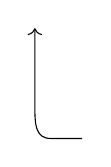
\begin{tikzpicture}\draw[->] (.6,0)--(.2,0) .. controls (0,0) and (0,.2) .. (0,.4)--(0,1.4);\end{tikzpicture}}}empty !

These reflections bring very near how much stronger the \var{\inserted{extra}}{\hand{extra}}{insertion}{ps_134-3_069-v0014} strictness
requi\var{\over[typed]{\unsure{t}}{r}}{r}{typewriter overwriting}{ps_134-3_069-v0015}ement T 2 for test categories, than merely the conditions T 1, T3
without T 2 .

40. Yesterday I incidentally made use of the fact that if A is an asphe-%
ric element in (Cat), th\var{\over[typed]{\unsure{a}}{e}}{e}{typewriter overwriting}{ps_134-3_069-v0016}n for any other object C, CxA \hand{\ensuremath{\longrightarrow}} C is aspheric
(and a fortiori a weak equivalence). The usual asphericity criterion for a
functor shows that it is enough to prove that for any C with final element,
\margin{\diagram{\begin{tikzpicture}\draw[->] (.6,1.4)--(.2,1.4) .. controls (0,1.4) and (0,1.2) .. (0,1)--(0,0);\end{tikzpicture}}}CxA is aspheric. \var{\xout{Thusxw}}{}{typewriter deletion}{ps_134-3_069-v0017} For this again it is enough to prove that the
projection CxA \hand{\ensuremath{\longrightarrow}} A is aspheric, which by localisation up\var{\over[typed]{n}{o}}{o}{typewriter overwriting}{ps_134-3_069-v0018}n A means that
the product categories \hand{.} Cx\hand{(}$A_{/a}$\hand{)} (with a in A) are aspheric. Finall\var{\over{\unsure{x}}{y}}{\hand{y}}{writing over}{ps_134-3_069-v0019} we
are reduced to checking that the product of two categories with final ele-%
ment is aspheric, which is trivial because such a category has itself a
final element.

The result just proved can be viewed as a particular case of the
following
\uline{Proposition} In (Cat), the cartesian product of two weak equivalences is
a weak equivalence.

%% END SOURCE ps_134-3_069
\ifnum\EditionMode=1
\psapparatusstart
\psentry{ps_134-3_069-v0001}{1}{writing over}{\over{a}{,}}{\hand{,}}{The superposed handwritten reading replaces the underlying reading.}
\psentry{ps_134-3_069-v0002}{2}{insertion}{\inserted{as}}{\hand{as}}{The handwritten insertion is incorporated at its indicated position; insertion brackets leave the running text.}
\psentry{ps_134-3_069-v0003}{3}{writing over}{\over{t}{d}}{\hand{d}}{The superposed handwritten reading replaces the underlying reading.}
\psentry{ps_134-3_069-v0004}{4}{typewriter overwriting}{\over[typed]{what}{which}}{which}{The superposed typed reading replaces the underlying reading.}
\psentry{ps_134-3_069-v0005}{5}{typewriter overwriting}{\over[typed]{t}{t}}{t}{The superposed typed reading replaces the underlying reading.}
\psentry{ps_134-3_069-v0006}{6}{typewriter overwriting}{\over[typed]{a}{2}}{2}{The superposed typed reading replaces the underlying reading.}
\psentry{ps_134-3_069-v0007}{7}{writing over}{\over{ill}{ould}}{\hand{ould}}{The superposed handwritten reading replaces the underlying reading.}
\psentry{ps_134-3_069-v0008}{8}{typewriter deletion}{\xout{subob}}{}{The typewriter strikes out this material; it leaves the corrected running text.}
\psentry{ps_134-3_069-v0009}{9}{typewriter overwriting}{\over[typed]{\unsure{q}}{a}}{a}{The superposed typed reading replaces the underlying reading.}
\psentry{ps_134-3_069-v0010}{10}{typewriter overwriting}{\over[typed]{t}{v}}{v}{The superposed typed reading replaces the underlying reading.}
\psentry{ps_134-3_069-v0011}{11}{typewriter overwriting}{\over[typed]{e}{o}}{o}{The superposed typed reading replaces the underlying reading.}
\psentry{ps_134-3_069-v0012}{12}{typewriter overwriting}{\over[typed]{t}{t}}{t}{The superposed typed reading replaces the underlying reading.}
\psentry{ps_134-3_069-v0013}{13}{typewriter overwriting}{\over[typed]{t}{t}}{t}{The superposed typed reading replaces the underlying reading.}
\psentry{ps_134-3_069-v0014}{14}{insertion}{\inserted{extra}}{\hand{extra}}{The handwritten insertion is incorporated at its indicated position; insertion brackets leave the running text.}
\psentry{ps_134-3_069-v0015}{15}{typewriter overwriting}{\over[typed]{\unsure{t}}{r}}{r}{The superposed typed reading replaces the underlying reading.}
\psentry{ps_134-3_069-v0016}{16}{typewriter overwriting}{\over[typed]{\unsure{a}}{e}}{e}{The superposed typed reading replaces the underlying reading.}
\psentry{ps_134-3_069-v0017}{17}{typewriter deletion}{\xout{Thusxw}}{}{The typewriter strikes out this material; it leaves the corrected running text.}
\psentry{ps_134-3_069-v0018}{18}{typewriter overwriting}{\over[typed]{n}{o}}{o}{The superposed typed reading replaces the underlying reading.}
\psentry{ps_134-3_069-v0019}{19}{writing over}{\over{\unsure{x}}{y}}{\hand{y}}{The superposed handwritten reading replaces the underlying reading.}
\psapparatusend
\fi
\pssource{ps_134-3_070}{134-3/70}{https://grothendieck.umontpellier.fr/web/viewer.html?file=../134-3.pdf\#page=71}
\psnumber{ps_134-3_070-v0001}{1}
\psnumber{ps_134-3_070-v0002}{2}
\psnumber{ps_134-3_070-v0003}{3}
\psnumber{ps_134-3_070-v0004}{4}
\psnumber{ps_134-3_070-v0005}{5}
\psnumber{ps_134-3_070-v0006}{6}
\psnumber{ps_134-3_070-v0007}{7}
\psnumber{ps_134-3_070-v0008}{8}
%% BEGIN SOURCE ps_134-3_070
% Pursuing Stacks (cotes 134-2 to 134-8): archive cote 134-3, site page 70 (PDF page 71), typescript page 70.
% typescript. Draft compared: ps2.tex:3616-3680.
% AI-transcribed by Claude Opus 5.5 (claude-opus-5-5, adaptive thinking, effort high), Message Batches API, batch ps1 (msgbatch_01Rv5hCaNTtUt4JHx1yqoHPL), 2026-11-12; image review recorded in records/CHECK_DECISIONS_134_3_4.tsv.
\scanpage{134-3/70}
\mspage{\hand{70}}

(We get the previous result by taking the weak equivalences $A\hand{\to} e_{(Cat)}$
and $id_C : C \hand{\to} C$.)  To prove the proposition,  we are immediately reduced
to the case when one of the two functors is \var{\xout{the}}{}{typewriter deletion}{ps_134-3_070-v0001} an identity functork  i.e.
proving the
\uline{Corollary 1}  If  $f$:  $A'\hand{\to} A$ is a weak equivalence in (Cat),  then for any
\var{\over{\unsure{E}}{C}}{\hand{C}}{writing over}{ps_134-3_070-v0002} in (Cat)  $f\hand{x}id_{\hand{C}}$ : $A'xC \hand{\to} AxC$  is a weak equivalence.

For proving this,  we view the functor $fxid_C$  as a morphism of catego-%
ries ``over C'',  which corresponds to a situation of a morphism of topo\var{\over[typed]{i}{i}}{i}{typewriter overwriting}{ps_134-3_070-v0003}
over a third one
% Hand-drawn arrows are marked blue; typed objects remain plain.
\diagram{\begin{tikzcd}[column sep=tiny]
X' \ar[color=blue,rr,"f"] \ar[color=blue,dr] \& \& X \ar[color=blue,dl] \\
\& Y \&
\end{tikzcd}}
\qquad ,

we will say that $f$ is a \uline{weak equivalence} \uline{relative to} $Y$ ,  if not only this
is a weak equivalence,  but remain\hand{s} so by any base change by a localization
functor
\[ Y_{/U} \hand{\to} U \]
giving rise to
\[ f_{/U} : X'_{/U} \hand{\to} X_{/U} \qquad . \]
As usual,  standar\var{\over{t}{d}}{\hand{d}}{writing over}{ps_134-3_070-v0004} arguments prove that it is enough to take $U$ in a set
of generators of the topos $Y$ .  In case $Y$ =  $C^{\hand{\overset{\wedge}{\wedge}}}$ ,  we may take $U$ in $C$ .
In case moreover  $X,X'$ are defined by sm\var{\over[typed]{\unsure{m}}{a}}{a}{typewriter overwriting}{ps_134-3_070-v0005}ll categories $P,P'$ and a functor
of categories over $C$
\diagram{\begin{tikzcd}[column sep=tiny]
P' \ar[color=blue,rr,"F"] \ar[color=blue,dr] \& \& P \ar[color=blue,dl] \\
\& C \&
\end{tikzcd}}
\qquad ,

this condition amounts to demanding that for any $c$ in $C$,  the induced func-%
tor
\[ F_{/c} : P'_{/c} \hand{\to} P_{/c} \]
be a weak equivalence.  In our case $P=AxC,P'=A'xC$, $F = fxid_C$ ,  the indu-%
ced functor can be identified with  $fx\,id_{C_{/c}}$  .  This reduces us,  for
proving the corollary, to the case when $C$ has a final element.  But consi-%
der now the commutative diagram
\diagram{\begin{tikzcd}
A'xC \ar[color=blue,r,"\hand{fxid_c}"] \ar[color=blue,d] \& A\var{\deleted{'}}{}{deletion}{ps_134-3_070-v0006}xC \ar[color=blue,d] \\
A' \ar[color=blue,r,"\hand{f}"] \& A
\end{tikzcd}}
\qquad ,
where the vertical arrows are the projections and hence,  by what was
proved before,  weak equivalences.  As $f$ is a weak equivalence,  it follows
that $fxid_C$ is a weak equivalence too,  qed.

T\var{\over[typed]{h}{h}}{h}{typewriter overwriting}{ps_134-3_070-v0007}e proposition above goes somewhat in the direction of looking at
``homotopy properties of (Cat)''  \var{\deleted{\illegible{1}}}{}{deletion}{ps_134-3_070-v0008} and ``how far (Cat) is from being a
closed model category in Quillen's sense''.  It is very suggestive \hand{for}

%% END SOURCE ps_134-3_070
\ifnum\EditionMode=1
\psapparatusstart
\psentry{ps_134-3_070-v0001}{1}{typewriter deletion}{\xout{the}}{}{The typewriter strikes out this material; it leaves the corrected running text.}
\psentry{ps_134-3_070-v0002}{2}{writing over}{\over{\unsure{E}}{C}}{\hand{C}}{The superposed handwritten reading replaces the underlying reading.}
\psentry{ps_134-3_070-v0003}{3}{typewriter overwriting}{\over[typed]{i}{i}}{i}{The superposed typed reading replaces the underlying reading.}
\psentry{ps_134-3_070-v0004}{4}{writing over}{\over{t}{d}}{\hand{d}}{The superposed handwritten reading replaces the underlying reading.}
\psentry{ps_134-3_070-v0005}{5}{typewriter overwriting}{\over[typed]{\unsure{m}}{a}}{a}{The superposed typed reading replaces the underlying reading.}
\psentry{ps_134-3_070-v0006}{6}{deletion}{$\deleted{'}$}{}{The author cancels this material by hand; it leaves the corrected running text.}
\psentry{ps_134-3_070-v0007}{7}{typewriter overwriting}{\over[typed]{h}{h}}{h}{The superposed typed reading replaces the underlying reading.}
\psentry{ps_134-3_070-v0008}{8}{deletion}{\deleted{\illegible{1}}}{}{The author cancels this material by hand; it leaves the corrected running text.}
\psapparatusend
\fi
\pssource{ps_134-3_071}{134-3/71}{https://grothendieck.umontpellier.fr/web/viewer.html?file=../134-3.pdf\#page=72}
\psnumber{ps_134-3_071-v0001}{1}
\psnumber{ps_134-3_071-v0002}{2}
\psnumber{ps_134-3_071-v0003}{3}
\psnumber{ps_134-3_071-v0004}{4}
\psnumber{ps_134-3_071-v0005}{5}
\psnumber{ps_134-3_071-v0006}{6}
\psnumber{ps_134-3_071-v0007}{7}
\psnumber{ps_134-3_071-v0008}{8}
\psnumber{ps_134-3_071-v0009}{9}
\psnumber{ps_134-3_071-v0010}{10}
\psnumber{ps_134-3_071-v0011}{11}
\psnumber{ps_134-3_071-v0012}{12}
\psnumber{ps_134-3_071-v0013}{13}
\psnumber{ps_134-3_071-v0014}{14}
\psnumber{ps_134-3_071-v0015}{15}
\psnumber{ps_134-3_071-v0016}{16}
\psnumber{ps_134-3_071-v0017}{17}
\psnumber{ps_134-3_071-v0018}{18}
\psnumber{ps_134-3_071-v0019}{19}
\psnumber{ps_134-3_071-v0020}{20}
\psnumber{ps_134-3_071-v0021}{21}
\psnumber{ps_134-3_071-v0022}{22}
\psnumber{ps_134-3_071-v0023}{23}
\psnumber{ps_134-3_071-v0024}{24}
%% BEGIN SOURCE ps_134-3_071
% Pursuing Stacks (cotes 134-2 to 134-8): archive cote 134-3, site page 71 (PDF page 72), typescript page 71.
% typescript. Draft compared: ps2.tex:3667-3729.
% AI-transcribed by Claude Opus 5.5 (claude-opus-5-5, adaptive thinking, effort high), Message Batches API, batch ps1 (msgbatch_01Rv5hCaNTtUt4JHx1yqoHPL), 2026-11-12; image review recorded in records/CHECK_DECISIONS_134_3_4.tsv.
\scanpage{134-3/71}
\mspage{71}
having a closer look at \var{\deleted{functors}}{}{deletion}{ps_134-3_071-v0001} \var{\inserted{maps}}{\hand{maps}}{insertion}{ps_134-3_071-v0002} f: $\var{\over{B}{B}}{\hand{B}}{writing over}{ps_134-3_071-v0003}^{\var{\deleted{\illegible{1}}}{}{deletion}{ps_134-3_071-v0004}}\hand{\to}$ A in (Cat) which are ``universal
\margin{X awkward}weak equivalences'' i.e. $W_{(\mathrm{Cat})}$ -aspheric\var{\inserted{(46)}}{\hand{(46)}}{insertion}{ps_134-3_071-v0005}, namely such that for \uline{any} map
in (Cat) $A'\hand{\to}A$ (not only a localization\var{\deleted{x}}{}{deletion}{ps_134-3_071-v0006} $A_{/a}\hand{\to}A$), the induced
functor $B'=B\mathrm{x}_A A'\hand{\to}A'$ is a weak equivalence. This property is a lot
stronger than just asphericity, and reminds of the ``trivial fibrations''
in Quillens theory. The usual criterion af asphericity for $B'\hand{\to}A'$ shows
that f is W-aspheric iff \var{\deleted{if}}{}{deletion}{ps_134-3_071-v0007} for any A' with final element, and any func-%
tor $A'\hand{\to}A$, the fiber product $B'=B\mathrm{x}_A A'$ is aspheric. T\var{\over[typed]{h}{h}}{h}{typewriter overwriting}{ps_134-3_071-v0008}e feeling here is
(suggested partly by Quillen's terminology) that this property is tied up
some way with the property for f to be a fibering(or cofibering ?) functor,
in the sense of fibered and cofibered categories, with aspheric fibers
moreover. Presumably fibered or cofibered categories \var{\inserted{[in the purely categorical sense]}}{\hand{[in the purely categorical sense]}}{insertion}{ps_134-3_071-v0009}, with``base change
functors'' which are weak equivalences, will play the part of Serre-Quil-%
len's fibrations - and it is still to be guessed what kind of \var{\deleted{categorical}}{}{deletion}{ps_134-3_071-v0010}
properties of a functor will play the part of \uline{co}fibrations. Apparently
they will have to be a lot more stringent than just monomorphisms in (Cat),
cf. \var{\deleted{p. 37.}}{}{deletion}{ps_134-3_071-v0011} \hand{Section 30 [and (9)]}.

\margin{\diagram{\begin{tikzpicture}\draw[->] (.6,0)--(.2,0) .. controls (0,0) and (0,.2) .. (0,.4)--(0,1.3);\end{tikzpicture}}}H\var{\over[typed]{e}{o}}{o}{typewriter overwriting}{ps_134-3_071-v0012}\var{\over[typed]{w}{w}}{w}{typewriter overwriting}{ps_134-3_071-v0013}ever I feel it is not time yet to dive into the homotopy theory
properties of the all-encompassing basic modelizer (Cat), but rather come
back to the study of general (and less gene\var{\over[typed]{f}{r}}{r}{typewriter overwriting}{ps_134-3_071-v0014}al) test categories.

\margin{\diagram{\begin{tikzpicture}\draw[->] (.6,1.3)--(.2,1.3) .. controls (0,1.3) and (0,1.1) .. (0,.9)--(0,0);\end{tikzpicture}}}41. One comment \var{\inserted{still,}}{\hand{still,}}{insertion}{ps_134-3_071-v0015} upon the role played in the theory I am developping of
the \hand{``}assumption\hand{''}\allowbreak{}(p.30) that the category of autoequivalences of (Hot) is
equivalent to the final category. This assumption has been a crucial
guide for putting the emphasis where it really belongs, namely upon
the set \var{\deleted{of}}{}{deletion}{ps_134-3_071-v0016} $W\hand{\subset}\mathrm{Fl}(M)$ of weak equivalences within a category M which one
would like to take in some sense as a category of models for homotopy
types - the functors $M\hand{\to}$(Hot) following along auto\var{\over[typed]{h}{m}}{m}{typewriter overwriting}{ps_134-3_071-v0017}atically. However,
in no statement whatever I proved so far, was this assumption ever used\var{\over{.}{!}}{\hand{!}}{writing over}{ps_134-3_071-v0018}
\var{\deleted{However,}}{}{deletion}{ps_134-3_071-v0019}\var{\inserted{On the other hand,}}{\hand{On the other hand,}}{insertion}{ps_134-3_071-v0020} the notion of a \uline{modelizer} introduced in the wake of the \hand{``}assumpti-%
on\hand{''} (cf. \hand{\S.28}) was tacitly changed during the reflection, by drapping al-%
together the condition a) of (strong) saturation of W, namely that W is
just the set of arrows\unsure{\hand{,}} made invertible by the localization functor $M\hand{\to}W^{-1}M$.
Instead of this, it turned out that the saturation condition we really had
at hands and which \var{\xout{were}}{}{typewriter deletion}{ps_134-3_071-v0021} was adequate for working, was the conditions
a) to c) I finally wrote \var{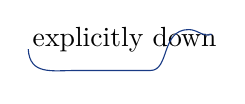
\begin{tikzpicture}[baseline=(t.base)]\node[anchor=base west,inner sep=0pt] (t) at (0,0) {explicitly down};\draw[color=blue] (-.05,-.03) .. controls (-.03,-.36) and (.25,-.30) .. (.55,-.30)--(1.50,-.30) .. controls (1.75,-.30) and (1.63,.22) .. (1.99,.22) .. controls (2.10,.22) and (2.17,.12) .. (2.28,.16);\end{tikzpicture}}{down explicitly}{authorial transposition}{ps_134-3_071-v0022} yesterday (\hand{\S.37}). As for the
strong saturation condition, for the time being (using nothing but what
has actually be\var{\inserted{en}}{\hand{en}}{insertion}{ps_134-3_071-v0023} proved\var{\deleted{\illegible{1}}}{}{deletion}{ps_134-3_071-v0024} so far, without reference to ``well known facts''
from homotopy theory)\hand{,} it is not even clear that the basic modelizer
(Cat) is one in the initial sense, namely that the set of weak equivalen-

%% END SOURCE ps_134-3_071
\ifnum\EditionMode=1
\psapparatusstart
\psentry{ps_134-3_071-v0001}{1}{deletion}{\deleted{functors}}{}{The author cancels this material by hand; it leaves the corrected running text.}
\psentry{ps_134-3_071-v0002}{2}{insertion}{\inserted{maps}}{\hand{maps}}{The handwritten insertion is incorporated at its indicated position; insertion brackets leave the running text.}
\psentry{ps_134-3_071-v0003}{3}{writing over}{$\over{B}{B}$}{$\hand{B}$}{The superposed handwritten reading replaces the underlying reading.}
\psentry{ps_134-3_071-v0004}{4}{deletion}{$\deleted{\illegible{1}}$}{}{The author cancels this material by hand; it leaves the corrected running text.}
\psentry{ps_134-3_071-v0005}{5}{insertion}{\inserted{(46)}}{\hand{(46)}}{The handwritten insertion is incorporated at its indicated position; insertion brackets leave the running text.}
\psentry{ps_134-3_071-v0006}{6}{deletion}{\deleted{x}}{}{The author cancels this material by hand; it leaves the corrected running text.}
\psentry{ps_134-3_071-v0007}{7}{deletion}{\deleted{if}}{}{The author cancels this material by hand; it leaves the corrected running text.}
\psentry{ps_134-3_071-v0008}{8}{typewriter overwriting}{\over[typed]{h}{h}}{h}{The superposed typed reading replaces the underlying reading.}
\psentry{ps_134-3_071-v0009}{9}{insertion}{\inserted{[in the purely categorical sense]}}{\hand{[in the purely categorical sense]}}{The handwritten insertion is incorporated at its indicated position; insertion brackets leave the running text.}
\psentry{ps_134-3_071-v0010}{10}{deletion}{\deleted{categorical}}{}{The author cancels this material by hand; it leaves the corrected running text.}
\psentry{ps_134-3_071-v0011}{11}{deletion}{\deleted{p. 37.}}{}{The author cancels this material by hand; it leaves the corrected running text.}
\psentry{ps_134-3_071-v0012}{12}{typewriter overwriting}{\over[typed]{e}{o}}{o}{The superposed typed reading replaces the underlying reading.}
\psentry{ps_134-3_071-v0013}{13}{typewriter overwriting}{\over[typed]{w}{w}}{w}{The superposed typed reading replaces the underlying reading.}
\psentry{ps_134-3_071-v0014}{14}{typewriter overwriting}{\over[typed]{f}{r}}{r}{The superposed typed reading replaces the underlying reading.}
\psentry{ps_134-3_071-v0015}{15}{insertion}{\inserted{still,}}{\hand{still,}}{The handwritten insertion is incorporated at its indicated position; insertion brackets leave the running text.}
\psentry{ps_134-3_071-v0016}{16}{deletion}{\deleted{of}}{}{The author cancels this material by hand; it leaves the corrected running text.}
\psentry{ps_134-3_071-v0017}{17}{typewriter overwriting}{\over[typed]{h}{m}}{m}{The superposed typed reading replaces the underlying reading.}
\psentry{ps_134-3_071-v0018}{18}{writing over}{\over{.}{!}}{\hand{!}}{The superposed handwritten reading replaces the underlying reading.}
\psentry{ps_134-3_071-v0019}{19}{deletion}{\deleted{However,}}{}{The author cancels this material by hand; it leaves the corrected running text.}
\psentry{ps_134-3_071-v0020}{20}{insertion}{\inserted{On the other hand,}}{\hand{On the other hand,}}{The handwritten insertion is incorporated at its indicated position; insertion brackets leave the running text.}
\psentry{ps_134-3_071-v0021}{21}{typewriter deletion}{\xout{were}}{}{The typewriter strikes out this material; it leaves the corrected running text.}
\psentry{ps_134-3_071-v0022}{22}{authorial transposition}{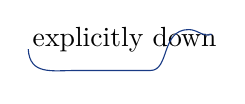
\begin{tikzpicture}[baseline=(t.base)]\node[anchor=base west,inner sep=0pt] (t) at (0,0) {explicitly down};\draw[color=blue] (-.05,-.03) .. controls (-.03,-.36) and (.25,-.30) .. (.55,-.30)--(1.50,-.30) .. controls (1.75,-.30) and (1.63,.22) .. (1.99,.22) .. controls (2.10,.22) and (2.17,.12) .. (2.28,.16);\end{tikzpicture}}{down explicitly}{The continuous pen curve under explicitly and over the beginning of down exchanges their typed order. Diplomatic retains the typed order and the graphic.}
\psentry{ps_134-3_071-v0023}{23}{insertion}{\inserted{en}}{\hand{en}}{The handwritten insertion is incorporated at its indicated position; insertion brackets leave the running text.}
\psentry{ps_134-3_071-v0024}{24}{deletion}{\deleted{\illegible{1}}}{}{The author cancels this material by hand; it leaves the corrected running text.}
\psapparatusend
\fi
\pssource{ps_134-3_072}{134-3/72}{https://grothendieck.umontpellier.fr/web/viewer.html?file=../134-3.pdf\#page=73}
\psnumber{ps_134-3_072-v0001}{1}
\psnumber{ps_134-3_072-v0002}{2}
\psnumber{ps_134-3_072-v0003}{3}
\psnumber{ps_134-3_072-v0004}{4}
\psnumber{ps_134-3_072-v0005}{5}
\psnumber{ps_134-3_072-v0006}{6}
\psnumber{ps_134-3_072-v0007}{7}
\psnumber{ps_134-3_072-v0008}{8}
\psnumber{ps_134-3_072-v0009}{9}
\psnumber{ps_134-3_072-v0010}{10}
\psnumber{ps_134-3_072-v0011}{11}
\psnumber{ps_134-3_072-v0012}{12}
\psnumber{ps_134-3_072-v0013}{13}
\psnumber{ps_134-3_072-v0014}{14}
\psnumber{ps_134-3_072-v0015}{15}
\psnumber{ps_134-3_072-v0016}{16}
\psnumber{ps_134-3_072-v0017}{17}
\psnumber{ps_134-3_072-v0018}{18}
\psnumber{ps_134-3_072-v0019}{19}
%% BEGIN SOURCE ps_134-3_072
% Pursuing Stacks (cotes 134-2 to 134-8): archive cote 134-3, site page 72 (PDF page 73), typescript page 72.
% typescript. Draft compared: ps2.tex:3717-3785.
% AI-transcribed by Claude Opus 5.5 (claude-opus-5-5, adaptive thinking, effort high), Message Batches API, batch ps1 (msgbatch_01Rv5hCaNTtUt4JHx1yqoHPL), 2026-11-12; image review recorded in records/CHECK_DECISIONS_134_3_4.tsv.
\scanpage{134-3/72}
\mspage{\hand{72}}

\margin{$\ast$ cf \unsure{th} p. \uline{VIII}}ces in (Cat) is strongly saturated\hand{(47)}\hand{.} However, from the known relation
between Cat and an elementary modelizer $A^{\hand{\wedge}}$, it follows that $W_{(\mathrm{Cat})}$ is
strongly saturated iff $W_A \hand{\subset} \mathrm{Fl}(A\var{\over{\unsure{?}}{{}^{\wedge}}}{\hand{{}^{\wedge}}}{writing over}{ps_134-3_072-v0001})$ is. This implies that it is enough to
prove strong saturation in \uline{one} elementary modelizer $A^{\hand{\wedge}}$, to deduce it in
all others, as well as in (Cat). However, in the case at least when
$A = \hand{\Delta}$, it is indeed "well-known" that \var{\inserted[typed]{the}}{the}{typed insertion}{ps_134-3_072-v0002} weak equivalences in $A^{\hand{\wedge}}$ satisfy the
strong saturation condition. In\var{\deleted{t}}{}{deletion}{ps_134-3_072-v0003} terms of Quillen's set-up, it follows
from the fact that $\hand{\Delta}^{\hand{\wedge}}$ is a "closed model category" , and prop.1 in I 5.5.
of Quillen's expos\'e. The only thing which is not quite understood, not by
me at any rate, is why $\hand{\Delta}^{\hand{\wedge}}$ \uline{is} indeed a closed model category - Quillen\hand{'}s
proof it seems relies strongly on typical simplicial techniques. I'll have
to look if the present set-up will suggest a more conceptual proof, valid
possibly for any test category (or at least, any strict test category).
I'll have to come back upon this later\hand{.} \var{\xout{after}}{}{typewriter deletion}{ps_134-3_072-v0004} For the time being, I feel
a greater urge still to understand about the relationship between different
test categories\hand{,} - also\hand{,} I did not really finish with my review of what
may be viewed as \var{\inserted{the}}{\hand{the}}{insertion}{ps_134-3_072-v0005} "standart\hand{"} test categories\var{\deleted{"}}{}{deletion}{ps_134-3_072-v0006} such as $\hand{\Delta}$, $\hand{\square}$ and their vari-%
ants.

25.3.

42. In the notes last time I made clear what finally has turned out for
me to correspond to the appelation of a "modelizer", as prompted by the
internal logics of the situations I was looking at, in terms of the infor-%
mation available to me. I should by then have added what a \uline{model-preser-}%
\uline{ving} \var{\inserted{(or \uline{modelizing})}}{\hand{(or \uline{modelizing})}}{insertion}{ps_134-3_072-v0007} \uline{functor} between modelizers (M,W) and (M',W') has turned out to mean,
which has undergone a corresponding change with respect \var{\xout{of}}{}{typewriter deletion}{ps_134-3_072-v0008} to what I first
contemplated calling by that name (\hand{\S.28}). Namely here it turned out that
I should be more stringent for this notion, replacing the condition
$f(W) \hand{\subset} W'$ by the stronger one
\[ W = f^{-1}(W') \quad , \]
and moreover, of course, still demanding that the corresponding functor
\[ W^{-1}M \hand{\to} W'^{-1}M' \]
should be an equivalence. It is by now established \var{\deleted{that}}{}{deletion}{ps_134-3_072-v0009}, with \var{\inserted[typed]{the}}{the}{typed insertion}{ps_134-3_072-v0010} \var{\xout{one}}{}{typewriter deletion}{ps_134-3_072-v0011} excep-%
tion of just \var{\inserted[typed]{the two}}{the two}{typed insertion}{ps_134-3_072-v0012} \var{\xout{one}}{}{typewriter deletion}{ps_134-3_072-v0013}, \var{\inserted[typed]{first,}}{first,}{typed insertion}{ps_134-3_072-v0014} \var{\inserted{that,}}{\hand{that,}}{insertion}{ps_134-3_072-v0015} all the functors occuring in the diagram on p.31 are
indeed model\var{\xout{izing}}{}{typewriter deletion}{ps_134-3_072-v0016} preserving, namely it is so for $\hand{\alpha}$, $\hand{\beta}$, $\hand{\xi}$, $\hand{\eta}$ - and also
the right adjoints to $\hand{\xi}$, $\hand{\eta}$, as expected by then. It should be more or \var{\xout{xx}}{}{typewriter deletion}{ps_134-3_072-v0017}
less trivial that the first of the functors in this diagram, namely
the canonical inclusion (Ord)$\hand{\longrightarrow}$(Preord), as well as the left adjoint
from (Preord) to (Ord), are model preserving - except for the fact that it
has not been yet established that these two categories are indeed modeli\var{\xout{xx}}{}{typewriter deletion}{ps_134-3_072-v0018}
zers (for the natural notion of weak equivalences, induce\var{\over[typed]{s}{d}}{d}{typewriter overwriting}{ps_134-3_072-v0019} from (Cat))\hand{,}

%% END SOURCE ps_134-3_072
\ifnum\EditionMode=1
\psapparatusstart
\psentry{ps_134-3_072-v0001}{1}{writing over}{$\over{\unsure{?}}{{}^{\wedge}}$}{$\hand{{}^{\wedge}}$}{The superposed handwritten reading replaces the underlying reading.}
\psentry{ps_134-3_072-v0002}{2}{typed insertion}{\inserted[typed]{the}}{the}{The typed insertion is incorporated at its indicated position; insertion brackets leave the running text.}
\psentry{ps_134-3_072-v0003}{3}{deletion}{\deleted{t}}{}{The author cancels this material by hand; it leaves the corrected running text.}
\psentry{ps_134-3_072-v0004}{4}{typewriter deletion}{\xout{after}}{}{The typewriter strikes out this material; it leaves the corrected running text.}
\psentry{ps_134-3_072-v0005}{5}{insertion}{\inserted{the}}{\hand{the}}{The handwritten insertion is incorporated at its indicated position; insertion brackets leave the running text.}
\psentry{ps_134-3_072-v0006}{6}{deletion}{\deleted{"}}{}{The author cancels this material by hand; it leaves the corrected running text.}
\psentry{ps_134-3_072-v0007}{7}{insertion}{\inserted{(or \uline{modelizing})}}{\hand{(or \uline{modelizing})}}{The handwritten insertion is incorporated at its indicated position; insertion brackets leave the running text.}
\psentry{ps_134-3_072-v0008}{8}{typewriter deletion}{\xout{of}}{}{The typewriter strikes out this material; it leaves the corrected running text.}
\psentry{ps_134-3_072-v0009}{9}{deletion}{\deleted{that}}{}{The author cancels this material by hand; it leaves the corrected running text.}
\psentry{ps_134-3_072-v0010}{10}{typed insertion}{\inserted[typed]{the}}{the}{The typed insertion is incorporated at its indicated position; insertion brackets leave the running text.}
\psentry{ps_134-3_072-v0011}{11}{typewriter deletion}{\xout{one}}{}{The typewriter strikes out this material; it leaves the corrected running text.}
\psentry{ps_134-3_072-v0012}{12}{typed insertion}{\inserted[typed]{the two}}{the two}{The typed insertion is incorporated at its indicated position; insertion brackets leave the running text.}
\psentry{ps_134-3_072-v0013}{13}{typewriter deletion}{\xout{one}}{}{The typewriter strikes out this material; it leaves the corrected running text.}
\psentry{ps_134-3_072-v0014}{14}{typed insertion}{\inserted[typed]{first,}}{first,}{The typed insertion is incorporated at its indicated position; insertion brackets leave the running text.}
\psentry{ps_134-3_072-v0015}{15}{insertion}{\inserted{that,}}{\hand{that,}}{The handwritten insertion is incorporated at its indicated position; insertion brackets leave the running text.}
\psentry{ps_134-3_072-v0016}{16}{typewriter deletion}{\xout{izing}}{}{The typewriter strikes out this material; it leaves the corrected running text.}
\psentry{ps_134-3_072-v0017}{17}{typewriter deletion}{\xout{xx}}{}{The typewriter strikes out this material; it leaves the corrected running text.}
\psentry{ps_134-3_072-v0018}{18}{typewriter deletion}{\xout{xx}}{}{The typewriter strikes out this material; it leaves the corrected running text.}
\psentry{ps_134-3_072-v0019}{19}{typewriter overwriting}{\over[typed]{s}{d}}{d}{The superposed typed reading replaces the underlying reading.}
\psapparatusend
\fi
\pssource{ps_134-3_073}{134-3/73}{https://grothendieck.umontpellier.fr/web/viewer.html?file=../134-3.pdf\#page=74}
\psnumber{ps_134-3_073-v0001}{1}
\psnumber{ps_134-3_073-v0002}{2}
\psnumber{ps_134-3_073-v0003}{3}
\psnumber{ps_134-3_073-v0004}{4}
\psnumber{ps_134-3_073-v0005}{5}
\psnumber{ps_134-3_073-v0006}{6}
\psnumber{ps_134-3_073-v0007}{7}
\psnumber{ps_134-3_073-v0008}{8}
\psnumber{ps_134-3_073-v0009}{9}
\psnumber{ps_134-3_073-v0010}{10}
\psnumber{ps_134-3_073-v0011}{11}
\psnumber{ps_134-3_073-v0012}{12}
\psnumber{ps_134-3_073-v0013}{13}
\psnumber{ps_134-3_073-v0014}{14}
\psnumber{ps_134-3_073-v0015}{15}
\psnumber{ps_134-3_073-v0016}{16}
\psnumber{ps_134-3_073-v0017}{17}
\psnumber{ps_134-3_073-v0018}{18}
\psnumber{ps_134-3_073-v0019}{19}
%% BEGIN SOURCE ps_134-3_073
% Pursuing Stacks (cotes 134-2 to 134-8): archive cote 134-3, site page 73 (PDF page 74), typescript page 73.
% typescript. Draft compared: ps2.tex:3773-3835.
% AI-transcribed by Claude Opus 5.5 (claude-opus-5-5, adaptive thinking, effort high), Message Batches API, batch ps1 (msgbatch_01Rv5hCaNTtUt4JHx1yqoHPL), 2026-11-12; image review recorded in records/CHECK_DECISIONS_134_3_4.tsv.
\scanpage{134-3/73}
\mspage{\hand{73}}

namely that the localized categories with respect to weak equivalences are
indeed equivalent to (Hot). T\var{\over[typed]{h}{h}}{h}{typewriter overwriting}{ps_134-3_073-v0001}e only natural way one might think of this
to be proved, is by proving that the inclusion functor from either into
(Cat) induces an equivalence between the localizations, which would imply
at the same time that th\var{\over[typed]{e}{i}}{i}{typewriter overwriting}{ps_134-3_073-v0002}s inclusion functor is indeed model-preserving,
and hence that all the functors in the diagram of p.31 are model preserving
functors between modelizers. I still do believe this should be so, and
want to give \var{\inserted[typed]{below}}{below}{typed insertion}{ps_134-3_073-v0003} a reflection which might lead to a proof of this.

Before, there is still one noteworthy circumstance I want to emphasize
% NOTE: the right edge of the scan cuts the ends of several typed lines (after "emphasize", "autoequi", "equi", "equivalenc")
Namely, it occured in a number of instances that we got in a rather natu-%
ral way several modelizing functors between \var{\inserted[typed]{two}}{two}{typed insertion}{ps_134-3_073-v0004} modelizers $(M,W)$ and $(M',W')$,
in one direction or the other - for instance from \var{\over{A}{(}}{\hand{(}}{writing over}{ps_134-3_073-v0005}Cat) to $A^{\hand{\wedge}}$ using
different functors $i: A \hand{\to} (Cat)$, or from $A^{\hand{\wedge}}$ to (Cat) using $a \hand{\mapsto} A_{/a}$ .
It turned out that the corresponding functors between $W^{-1}M$ and $W'^{-1}M'$ were
always canonically isomorphic \var{\deleted{if}}{}{deletion}{ps_134-3_073-v0006} \var{\inserted{when}}{\hand{when}}{insertion}{ps_134-3_073-v0007} in the same direction, \var{\over[typed]{\illegible{1}}{are}}{are}{typewriter overwriting}{ps_134-3_073-v0008} quasi-inverse
of each other \var{\deleted{if}}{}{deletion}{ps_134-3_073-v0009} \var{\inserted{when}}{\hand{when}}{insertion}{ps_134-3_073-v0010} in opposite directions. This is indeed very much in the
spirit of the``inspiring assumption'' of p.30, that the category of autoequi
valences of (Hot) is equivalent to the unit category, which implies indeed
that for two categories $H,H'$ equivalent to (Hot), \var{\xout{there exists a}}{}{typewriter deletion}{ps_134-3_073-v0011} for two equi
valences from $H$ to $H'$, there is a unique isomorphism between them. Quite
similarly, there have been a number of situations (more or less summed up
in the end in the ``key theorem'' of p.61) when \var{\inserted[typed]{by localization}}{by localization}{typed insertion}{ps_134-3_073-v0012} we got a natural functor $f$
from some $W^{-1}M$ to another $W'^{-1}M'$, and another \var{\inserted[typed]{$F$}}{$F$}{typed insertion}{ps_134-3_073-v0013} which is known already to be
an equivalence, and it turns out that $f$ is isomorphic to \var{\over[typed]{$f$}{$F$}}{$F$}{typewriter overwriting}{ps_134-3_073-v0014} (and in fact,
then, canonically so) iff f\unsure{\var{\over[typed]{ro}{or}}{or}{typewriter overwriting}{ps_134-3_073-v0015}} any object $x$ in the source category, $f(x)$
and $F(x)$ are isomorphic. This suggests that \uline{presumably}, \uline{every functor}
\uline{from} (Hot) \uline{into itself}, \uline{transforming every object into an isomorphic one},
\uline{is in fact isomorphic to the identity functor}.

I want now to make a comment, implying that there are many full sub-%
categories $M$ of (Cat), such that for the induced notion of weak equivalenc
$M$ becomes a modelizer, and the inclusion functor a modelizing functor -
or, what amount to the same, that the canonical functor
\[ {W_M}^{-1}M \hand{\longrightarrow} {W_{Cat}}^{-1}(Cat) = (Hot) \]
is an equivalence. To see this, let more generally $(M,W)$ be any catego-%
ry endowed with a subset $W \hand{\subset} Fl(M)$, and let $h: M \hand{\longrightarrow} M$ be a functor such
that $h(W) \hand{\subset} W$, and such that the induced functor $W^{-1}M \hand{\to} W^{-1}M$ is an equiva-%
lence. Let \var{\xout{on the other hand}}{}{typewriter deletion}{ps_134-3_073-v0016} \var{\inserted[typed]{now}}{now}{typed insertion}{ps_134-3_073-v0017} $M'$ be any full subcategory of $M$ such that
$h$ factors through $M'$ , let $h': M \hand{\to} M'$ be the corresponding \var{\inserted{induced}}{\hand{induced}}{insertion}{ps_134-3_073-v0018} functor, and
$W' = W \hand{\cap} Fl(M')$. Then it is formal that \var{\xout{h and h}}{}{typewriter deletion}{ps_134-3_073-v0019} the inclusion $g: M' \hand{\to} M$

%% END SOURCE ps_134-3_073
\ifnum\EditionMode=1
\psapparatusstart
\psentry{ps_134-3_073-v0001}{1}{typewriter overwriting}{\over[typed]{h}{h}}{h}{The superposed typed reading replaces the underlying reading.}
\psentry{ps_134-3_073-v0002}{2}{typewriter overwriting}{\over[typed]{e}{i}}{i}{The superposed typed reading replaces the underlying reading.}
\psentry{ps_134-3_073-v0003}{3}{typed insertion}{\inserted[typed]{below}}{below}{The typed insertion is incorporated at its indicated position; insertion brackets leave the running text.}
\psentry{ps_134-3_073-v0004}{4}{typed insertion}{\inserted[typed]{two}}{two}{The typed insertion is incorporated at its indicated position; insertion brackets leave the running text.}
\psentry{ps_134-3_073-v0005}{5}{writing over}{\over{A}{(}}{\hand{(}}{The superposed handwritten reading replaces the underlying reading.}
\psentry{ps_134-3_073-v0006}{6}{deletion}{\deleted{if}}{}{The author cancels this material by hand; it leaves the corrected running text.}
\psentry{ps_134-3_073-v0007}{7}{insertion}{\inserted{when}}{\hand{when}}{The handwritten insertion is incorporated at its indicated position; insertion brackets leave the running text.}
\psentry{ps_134-3_073-v0008}{8}{typewriter overwriting}{\over[typed]{\illegible{1}}{are}}{are}{The superposed typed reading replaces the underlying reading.}
\psentry{ps_134-3_073-v0009}{9}{deletion}{\deleted{if}}{}{The author cancels this material by hand; it leaves the corrected running text.}
\psentry{ps_134-3_073-v0010}{10}{insertion}{\inserted{when}}{\hand{when}}{The handwritten insertion is incorporated at its indicated position; insertion brackets leave the running text.}
\psentry{ps_134-3_073-v0011}{11}{typewriter deletion}{\xout{there exists a}}{}{The typewriter strikes out this material; it leaves the corrected running text.}
\psentry{ps_134-3_073-v0012}{12}{typed insertion}{\inserted[typed]{by localization}}{by localization}{The typed insertion is incorporated at its indicated position; insertion brackets leave the running text.}
\psentry{ps_134-3_073-v0013}{13}{typed insertion}{\inserted[typed]{$F$}}{$F$}{The typed insertion is incorporated at its indicated position; insertion brackets leave the running text.}
\psentry{ps_134-3_073-v0014}{14}{typewriter overwriting}{\over[typed]{$f$}{$F$}}{$F$}{The superposed typed reading replaces the underlying reading.}
\psentry{ps_134-3_073-v0015}{15}{typewriter overwriting}{\over[typed]{ro}{or}}{or}{The superposed typed reading replaces the underlying reading.}
\psentry{ps_134-3_073-v0016}{16}{typewriter deletion}{\xout{on the other hand}}{}{The typewriter strikes out this material; it leaves the corrected running text.}
\psentry{ps_134-3_073-v0017}{17}{typed insertion}{\inserted[typed]{now}}{now}{The typed insertion is incorporated at its indicated position; insertion brackets leave the running text.}
\psentry{ps_134-3_073-v0018}{18}{insertion}{\inserted{induced}}{\hand{induced}}{The handwritten insertion is incorporated at its indicated position; insertion brackets leave the running text.}
\psentry{ps_134-3_073-v0019}{19}{typewriter deletion}{\xout{h and h}}{}{The typewriter strikes out this material; it leaves the corrected running text.}
\psapparatusend
\fi
\pssource{ps_134-3_074}{134-3/74}{https://grothendieck.umontpellier.fr/web/viewer.html?file=../134-3.pdf\#page=75}
\psnumber{ps_134-3_074-v0001}{1}
\psnumber{ps_134-3_074-v0002}{2}
\psnumber{ps_134-3_074-v0003}{3}
\psnumber{ps_134-3_074-v0004}{4}
\psnumber{ps_134-3_074-v0005}{5}
\psnumber{ps_134-3_074-v0006}{6}
\psnumber{ps_134-3_074-v0007}{7}
\psnumber{ps_134-3_074-v0008}{8}
\psnumber{ps_134-3_074-v0009}{9}
\psnumber{ps_134-3_074-v0010}{10}
\psnumber{ps_134-3_074-v0011}{11}
\psnumber{ps_134-3_074-v0012}{12}
\psnumber{ps_134-3_074-v0013}{13}
\psnumber{ps_134-3_074-v0014}{14}
\psnumber{ps_134-3_074-v0015}{15}
\psnumber{ps_134-3_074-v0016}{16}
\psnumber{ps_134-3_074-v0017}{17}
\psnumber{ps_134-3_074-v0018}{18}
\psnumber{ps_134-3_074-v0019}{19}
\psnumber{ps_134-3_074-v0020}{20}
\psnumber{ps_134-3_074-v0021}{21}
\psnumber{ps_134-3_074-v0022}{22}
\psnumber{ps_134-3_074-v0023}{23}
\psnumber{ps_134-3_074-v0024}{24}
\psnumber{ps_134-3_074-v0025}{25}
\psnumber{ps_134-3_074-v0026}{26}
\psnumber{ps_134-3_074-v0027}{27}
%% BEGIN SOURCE ps_134-3_074
% Pursuing Stacks (cotes 134-2 to 134-8): archive cote 134-3, site page 74 (PDF page 75), typescript page 74.
% typescript. Draft compared: ps2.tex:3821-3890.
% AI-transcribed by Claude Opus 5.5 (claude-opus-5-5, adaptive thinking, effort high), Message Batches API, batch ps1 (msgbatch_01Rv5hCaNTtUt4JHx1yqoHPL), 2026-11-12; image review recorded in records/CHECK_DECISIONS_134_3_4.tsv.
\scanpage{134-3/74}
\mspage{\hand{74}}
and h'\var{\inserted{$:M\mathrel{\rule{.45cm}{.35pt}} M'$}}{\hand{$:M\mathrel{\rule{.45cm}{.35pt}} M'$}}{insertion}{ps_134-3_074-v0001} induce functors between $W'^{-1}M'$ and $W^{-1}M$, which are quasi-inverse
to each other - hence these two categories are equivalent. In case
(M,W) is a mode\unsure{\var{\over[typed]{h}{l}}{l}{typewriter overwriting}{ps_134-3_074-v0002}}izer, this implies that (M',W') is a modelizer too and the
\var{\inserted[typed]{inclusion}}{inclusion}{typed insertion}{ps_134-3_074-v0003} functor\var{\xout{s}}{}{typewriter deletion}{ps_134-3_074-v0004} g, as well as h', are model\var{\xout{s}}{}{typewriter deletion}{ps_134-3_074-v0005} preserving.

We can apply this remark to \var{\over[typed]{\unsure{M}}{t}}{t}{typewriter overwriting}{ps_134-3_074-v0006}he modelizer (Cat), and to the functor
\[ i_A\, i^{*} : (Cat) \hand{\longrightarrow} (Cat) \]
defined by any functor i: $A\hand{\longrightarrow}$ (Cat) satisfying the conditions of the
``key theorem'' (\hand{\S}. \var{\over{5}{3}}{\hand{3}}{writing over}{ps_134-3_074-v0007}\var{\over{7}{7}}{\hand{7}}{writing over}{ps_134-3_074-v0008}), for instance the functor $i_A\hand{|}A$ : $a\hand{\longmapsto} A_{/a}$
(where A is any test category). We get the following
\uline{Proposition} Let M be any full subcategory of (Cat), assume there exists
a test-category A such that for any F in $A^{\hand{\wedge}}$, the category $A_{/F}$ belongs to
M (i.e. the functor $i_A$ : $A^{\hand{\wedge}}\hand{\longrightarrow}$ (Cat) , $F\hand{\longmapsto} A_{/F}$ , factors through M). \var{\xout{Then}}{}{typewriter deletion}{ps_134-3_074-v0009}
Let $W_M$ be the set of weak equivalences in M . Then $(M,W_M)$ is a \var{\xout{test cate-}}{}{typewriter deletion}{ps_134-3_074-v0010}%
\var{\xout{gory}}{}{typewriter deletion}{ps_134-3_074-v0011} \var{\inserted[typed]{modelizer}}{modelizer}{typed insertion}{ps_134-3_074-v0012} and the inclusion functor $M\hand{\to}$ (Cat) is model preserving.

T\var{\over[typed]{h}{h}}{h}{typewriter overwriting}{ps_134-3_074-v0013}e same of course will be true for any full subcategory of (Cat) con-
taining M - which makes an impressive bunch of modelizers indeed ! When
\var{\inserted[typed]{the test category}}{the test category}{typed insertion}{ps_134-3_074-v0014} A is given, one natural choice for M is to take all categories \var{\inserted{C}}{\hand{C}}{insertion}{ps_134-3_074-v0015} which are
``locally isomorphic to A '' , namely such that for any x in C, the indu-
ced category $C_{/x}$ be isomorphic to a category of the type $A_{/a}$ , with a in
A .

It would be tempting to apply this result to the full subcategory
(Ord) of (Cat) - but for this to be feasible, would mean exactly that
there exists a test-category A defined by an ordered set \var{\inserted{\deleted{(or at least ``locally ordered'')}}}{\hand{}}{insertion}{ps_134-3_074-v0016}. To see whether
there exists indeed such an ordered set looks like a rather interesting
question - maybe it would give rise to \var{\inserted[typed]{algebraic}}{algebraic}{typed insertion}{ps_134-3_074-v0017} models for homotopy types, sim-
pler than those used so far, namely simplicial and cubical complexes and
multicomplexes. It is interesting to note that if such a test category
should exist, it will \uline{not} be in any case a strict test category. Indeed,
the topos $A^{\hand{\wedge}}$ associated to an ordered set A can be viewed also, as we saw
before (\hand{\S}.\var{\over{\unsure{1}}{2}}{\hand{2}}{writing over}{ps_134-3_074-v0018}\var{\over{2}{2}}{\hand{2}}{writing over}{ps_134-3_074-v0019}), as associated to \var{\inserted[typed]{a suitable}}{a suitable}{typed insertion}{ps_134-3_074-v0020} \var{\deleted{the}}{}{deletion}{ps_134-3_074-v0021} topological space (namely A endowed
with a suitable topology, the open sets being just the``cribles'' in A).
But we have seen that the topos associated to a topological space \uline{cannot}
be \uline{strictly} modelizing (\var{\inserted{prop.2,}}{\hand{prop.2,}}{insertion}{ps_134-3_074-v0022} cor.2 \var{\over{o}{i}}{\hand{i}}{writing over}{ps_134-3_074-v0023}n \var{\deleted{page 53}}{}{deletion}{ps_134-3_074-v0024} \var{\inserted{section 35}}{\hand{section 35}}{insertion}{ps_134-3_074-v0025}). \var{\begin{tikzpicture}[baseline=-.2ex]\draw[color=blue] (0,0)--(.25,0)--(.25,.4)--(.6,.4);\end{tikzpicture}}{

}{authorial paragraph break}{ps_134-3_074-v0026} This remark confirms the fee-
ling that it was worth while emphasizing the notion of a test category
\margin{X} (just T 1 + T 3 ) by a simple and striking name as I finally did, rather
than bury it behind the notion I now call a strict test category, which
is considerably more stringent and, moreover, more``rigid''. For instance,
it is not stable under localization $A_{/a}$ , whereas the notion of a test cate-
gory is - indeed, for any aspheric I in $A^{\hand{\wedge}}$, $A_{/I}$ is still a test categor\var{\over{y}{y}}{\hand{y}}{writing over}{ps_134-3_074-v0027}

%% END SOURCE ps_134-3_074
\ifnum\EditionMode=1
\psapparatusstart
\psentry{ps_134-3_074-v0001}{1}{insertion}{\inserted{$:M\mathrel{\rule{.45cm}{.35pt}} M'$}}{\hand{$:M\mathrel{\rule{.45cm}{.35pt}} M'$}}{The handwritten insertion is incorporated at its indicated position; insertion brackets leave the running text.}
\psentry{ps_134-3_074-v0002}{2}{typewriter overwriting}{\over[typed]{h}{l}}{l}{The superposed typed reading replaces the underlying reading.}
\psentry{ps_134-3_074-v0003}{3}{typed insertion}{\inserted[typed]{inclusion}}{inclusion}{The typed insertion is incorporated at its indicated position; insertion brackets leave the running text.}
\psentry{ps_134-3_074-v0004}{4}{typewriter deletion}{\xout{s}}{}{The typewriter strikes out this material; it leaves the corrected running text.}
\psentry{ps_134-3_074-v0005}{5}{typewriter deletion}{\xout{s}}{}{The typewriter strikes out this material; it leaves the corrected running text.}
\psentry{ps_134-3_074-v0006}{6}{typewriter overwriting}{\over[typed]{\unsure{M}}{t}}{t}{The superposed typed reading replaces the underlying reading.}
\psentry{ps_134-3_074-v0007}{7}{writing over}{\over{5}{3}}{\hand{3}}{The superposed handwritten reading replaces the underlying reading.}
\psentry{ps_134-3_074-v0008}{8}{writing over}{\over{7}{7}}{\hand{7}}{The superposed handwritten reading replaces the underlying reading.}
\psentry{ps_134-3_074-v0009}{9}{typewriter deletion}{\xout{Then}}{}{The typewriter strikes out this material; it leaves the corrected running text.}
\psentry{ps_134-3_074-v0010}{10}{typewriter deletion}{\xout{test cate-}}{}{The typewriter strikes out this material; it leaves the corrected running text.}
\psentry{ps_134-3_074-v0011}{11}{typewriter deletion}{\xout{gory}}{}{The typewriter strikes out this material; it leaves the corrected running text.}
\psentry{ps_134-3_074-v0012}{12}{typed insertion}{\inserted[typed]{modelizer}}{modelizer}{The typed insertion is incorporated at its indicated position; insertion brackets leave the running text.}
\psentry{ps_134-3_074-v0013}{13}{typewriter overwriting}{\over[typed]{h}{h}}{h}{The superposed typed reading replaces the underlying reading.}
\psentry{ps_134-3_074-v0014}{14}{typed insertion}{\inserted[typed]{the test category}}{the test category}{The typed insertion is incorporated at its indicated position; insertion brackets leave the running text.}
\psentry{ps_134-3_074-v0015}{15}{insertion}{\inserted{C}}{\hand{C}}{The handwritten insertion is incorporated at its indicated position; insertion brackets leave the running text.}
\psentry{ps_134-3_074-v0016}{16}{insertion}{\inserted{\deleted{(or at least ``locally ordered'')}}}{\hand{}}{The handwritten insertion is incorporated at its indicated position; insertion brackets leave the running text.}
\psentry{ps_134-3_074-v0017}{17}{typed insertion}{\inserted[typed]{algebraic}}{algebraic}{The typed insertion is incorporated at its indicated position; insertion brackets leave the running text.}
\psentry{ps_134-3_074-v0018}{18}{writing over}{\over{\unsure{1}}{2}}{\hand{2}}{The superposed handwritten reading replaces the underlying reading.}
\psentry{ps_134-3_074-v0019}{19}{writing over}{\over{2}{2}}{\hand{2}}{The superposed handwritten reading replaces the underlying reading.}
\psentry{ps_134-3_074-v0020}{20}{typed insertion}{\inserted[typed]{a suitable}}{a suitable}{The typed insertion is incorporated at its indicated position; insertion brackets leave the running text.}
\psentry{ps_134-3_074-v0021}{21}{deletion}{\deleted{the}}{}{The author cancels this material by hand; it leaves the corrected running text.}
\psentry{ps_134-3_074-v0022}{22}{insertion}{\inserted{prop.2,}}{\hand{prop.2,}}{The handwritten insertion is incorporated at its indicated position; insertion brackets leave the running text.}
\psentry{ps_134-3_074-v0023}{23}{writing over}{\over{o}{i}}{\hand{i}}{The superposed handwritten reading replaces the underlying reading.}
\psentry{ps_134-3_074-v0024}{24}{deletion}{\deleted{page 53}}{}{The author cancels this material by hand; it leaves the corrected running text.}
\psentry{ps_134-3_074-v0025}{25}{insertion}{\inserted{section 35}}{\hand{section 35}}{The handwritten insertion is incorporated at its indicated position; insertion brackets leave the running text.}
\psentry{ps_134-3_074-v0026}{26}{authorial paragraph break}{\begin{tikzpicture}[baseline=-.2ex]\draw[color=blue] (0,0)--(.25,0)--(.25,.4)--(.6,.4);\end{tikzpicture}}{

}{The stepped pen mark between the sentences calls for a paragraph break. Diplomatic retains the actual mark.}
\psentry{ps_134-3_074-v0027}{27}{writing over}{\over{y}{y}}{\hand{y}}{The superposed handwritten reading replaces the underlying reading.}
\psapparatusend
\fi
\pssource{ps_134-3_075}{134-3/75}{https://grothendieck.umontpellier.fr/web/viewer.html?file=../134-3.pdf\#page=76}
\psnumber{ps_134-3_075-v0001}{1}
\psnumber{ps_134-3_075-v0002}{2}
\psnumber{ps_134-3_075-v0003}{3}
\psnumber{ps_134-3_075-v0004}{4}
\psnumber{ps_134-3_075-v0005}{5}
\psnumber{ps_134-3_075-v0006}{6}
\psnumber{ps_134-3_075-v0007}{7}
\psnumber{ps_134-3_075-v0008}{8}
\psnumber{ps_134-3_075-v0009}{9}
\psnumber{ps_134-3_075-v0010}{10}
\psnumber{ps_134-3_075-v0011}{11}
\psnumber{ps_134-3_075-v0012}{12}
\psnumber{ps_134-3_075-v0013}{13}
\psnumber{ps_134-3_075-v0014}{14}
%% BEGIN SOURCE ps_134-3_075
% Pursuing Stacks (cotes 134-2 to 134-8): archive cote 134-3, site page 75 (PDF page 76), typescript page 75.
% typescript. Draft compared: ps2.tex:3875-3949.
% AI-transcribed by Claude Opus 5.5 (claude-opus-5-5, adaptive thinking, effort high), Message Batches API, batch ps1 (msgbatch_01Rv5hCaNTtUt4JHx1yqoHPL), 2026-11-12; image review recorded in records/CHECK_DECISIONS_134_3_4.tsv.
\scanpage{134-3/75}
\mspage{75}

43.   Now lets come back for \var{\over[typed]{a}{a}}{a}{typewriter overwriting}{ps_134-3_075-v0001} little while again to the so called ``standard
test categories'', and check how nicely the ``story retold'' applies to them.

N\hand{\ensuremath{\overset{\smile}{\textcolor{black}{o}}}}t speaking about multicomplexes, there are essentially two variants
for ``categories of simplices'' as test categories. The s\unsure{\var{\over[typed]{\illegible{2}}{ma}}{ma}{typewriter overwriting}{ps_134-3_075-v0002}}ller, more comm-%
monly used one, is the category $\hand{\Delta}$ of ``ordered simplices'', most convenient%
ly described as the full subcategory of (Cat) defined by the family of
simplices $\hand{\Delta}_n$ ($n \hand{\in} \underline{N}$). Here the most natural choice for i: $\hand{\Delta} \hand{\longrightarrow}$ (\var{\over[typed]{\unsure{U}}{C}}{C}{typewriter overwriting}{ps_134-3_075-v0003}at) is
of course the inclusion functor. \var{\deleted{The criterion for what might be called
``test-functors'' applies trivially here (cor. 3 of ``key theorem'', p.66),
\inserted[typed]{provided we check that}
thus \quad is indeed a test category and i a test-functor, \xout{moreover} \quad$_1$ to-%
gether with the usual \quad$_o$, \quad$_1$ is a homotopy interval in \quad. \xout{Also, the stan-}
\xout{dard criterion}}}{}{deletion}{ps_134-3_075-v0004} As i is fully faithful and $\hand{\Delta}_1$ is in the image, it follows
that $i^{\hand{*}}(\hand{\Delta}_1) = \hand{\Delta}_1$ , and we have only to check (for A to be a test-category
with ``test-functor'' i) that $\hand{\Delta}_1$ is \var{\xout{an}}{}{typewriter deletion}{ps_134-3_075-v0005} aspheric over $e=\hand{\Delta}_o$ , namely that
all products $\hand{\Delta}_1 \hand{\times} \hand{\Delta}_n$ are aspheric - which we did. The extra condition
of the``total asphericity criterion'' (proposition on \var{\over{\unsure{p. 67}}{\S. 39}}{\hand{\S. 39}}{writing over}{ps_134-3_075-v0006}), namely existen%
\hand{-}ce of a homotopy \var{\inserted{in $\Delta^{\wedge}$}}{\hand{in $\Delta^{\wedge}$}}{insertion}{ps_134-3_075-v0007} from the \var{\xout{constant}}{}{typewriter deletion}{ps_134-3_075-v0008} identity map to a constant map\hand{,} for any
$\hand{\Delta}_n$ , is indeed satisfied: \var{\xout{\illegible{1}}}{}{typewriter deletion}{ps_134-3_075-v0009}it \var{\xout{amounts to the same}}{}{typewriter deletion}{ps_134-3_075-v0010} \var{\inserted[typed]{is enough}}{is enough}{typed insertion}{ps_134-3_075-v0011} to define such homotopy
in (Cat), which is trivial using the final element of $\hand{\Delta}_n$ . Thus $\hand{\Delta}$ is
in fact a \uline{strict} test category.

As for $\hand{\widetilde{\Delta}}$ , the most elegant choice theoretically is to take the cate-%
gory of all non-empty finite sets, but this leads to set-theoretic diffi-%
culties, as \var{\over[typed]{A}{t}}{t}{typewriter overwriting}{ps_134-3_075-v0012}his category is not small - thus we take again the standard
non-ordered simplices
\[ \hand{\widetilde{\Delta}}_n = \underline{N} \hand{\cap} \hand{[}0,n\hand{]} \qquad (n \hand{\in} \underline{N}) \quad , \]
so as to get a ``reduced'' category with a countable set of objects. T\var{\over[typed]{h}{h}}{h}{typewriter overwriting}{ps_134-3_075-v0013}is
time, as $\hand{\widetilde{\Delta}}$ is stable under finite products, and contains the ``interval''
$(\hand{\widetilde{\Delta}}_1, \hand{\delta}_o, \hand{\delta}_1)$ (which is necessarily then a homotopy interval, as all ele-%
ments of $\hand{\widetilde{\Delta}}$ are aspheric over $e = \hand{\widetilde{\Delta}}_o$), the fact that $\hand{\Delta}$ is a strict test
category is trivial. As for a test functor, the neatest choice is the one
we said before, namely associating to every finite set the ordered set of
all non-empty subsets. We thus get
\[ \hand{\widetilde{\ }}i : \hand{\widetilde{\Delta}}\hand{\unsure{\ensuremath{{}^{\sim}}}} \hand{\longrightarrow} (Cat) \qquad \text{(factoring in fact through (Ord),} \]
\[ \text{as does } i: \hand{\Delta} \hand{\longrightarrow} \text{(Cat) above )} \]
To prove it is indeed a test functor, the corollary 3 to the ``key theorem''
(\var{\over{\unsure{p.66}}{\S.38}}{\hand{\S.38}}{writing over}{ps_134-3_075-v0014}) applies, taking of course I = $\hand{\widetilde{\Delta}}_1$ , hence
\[ \hand{\widetilde{\ }}i_{\hand{!}} (I) = i(\hand{\widetilde{\Delta}}_1 ) = \hand{\diagram{\begin{tikzcd}[row sep=small, column sep=small] \{1\} \ar[dr] \& \\ \& \{0,1\} \\ \{0\} \ar[ur] \& \end{tikzcd}}} \quad . \]

%% END SOURCE ps_134-3_075
\ifnum\EditionMode=1
\psapparatusstart
\psentry{ps_134-3_075-v0001}{1}{typewriter overwriting}{\over[typed]{a}{a}}{a}{The superposed typed reading replaces the underlying reading.}
\psentry{ps_134-3_075-v0002}{2}{typewriter overwriting}{\over[typed]{\illegible{2}}{ma}}{ma}{The superposed typed reading replaces the underlying reading.}
\psentry{ps_134-3_075-v0003}{3}{typewriter overwriting}{\over[typed]{\unsure{U}}{C}}{C}{The superposed typed reading replaces the underlying reading.}
\psentry{ps_134-3_075-v0004}{4}{deletion}{\deleted{The criterion for what might be called
``test-functors'' applies trivially here (cor. 3 of ``key theorem'', p.66),
\inserted[typed]{provided we check that}
thus \quad is indeed a test category and i a test-functor, \xout{moreover} \quad$_1$ to-%
gether with the usual \quad$_o$, \quad$_1$ is a homotopy interval in \quad. \xout{Also, the stan-}
\xout{dard criterion}}}{}{The author cancels this material by hand; it leaves the corrected running text.}
\psentry{ps_134-3_075-v0005}{5}{typewriter deletion}{\xout{an}}{}{The typewriter strikes out this material; it leaves the corrected running text.}
\psentry{ps_134-3_075-v0006}{6}{writing over}{\over{\unsure{p. 67}}{\S. 39}}{\hand{\S. 39}}{The superposed handwritten reading replaces the underlying reading.}
\psentry{ps_134-3_075-v0007}{7}{insertion}{\inserted{in $\Delta^{\wedge}$}}{\hand{in $\Delta^{\wedge}$}}{The handwritten insertion is incorporated at its indicated position; insertion brackets leave the running text.}
\psentry{ps_134-3_075-v0008}{8}{typewriter deletion}{\xout{constant}}{}{The typewriter strikes out this material; it leaves the corrected running text.}
\psentry{ps_134-3_075-v0009}{9}{typewriter deletion}{\xout{\illegible{1}}}{}{The typewriter strikes out this material; it leaves the corrected running text.}
\psentry{ps_134-3_075-v0010}{10}{typewriter deletion}{\xout{amounts to the same}}{}{The typewriter strikes out this material; it leaves the corrected running text.}
\psentry{ps_134-3_075-v0011}{11}{typed insertion}{\inserted[typed]{is enough}}{is enough}{The typed insertion is incorporated at its indicated position; insertion brackets leave the running text.}
\psentry{ps_134-3_075-v0012}{12}{typewriter overwriting}{\over[typed]{A}{t}}{t}{The superposed typed reading replaces the underlying reading.}
\psentry{ps_134-3_075-v0013}{13}{typewriter overwriting}{\over[typed]{h}{h}}{h}{The superposed typed reading replaces the underlying reading.}
\psentry{ps_134-3_075-v0014}{14}{writing over}{\over{\unsure{p.66}}{\S.38}}{\hand{\S.38}}{The superposed handwritten reading replaces the underlying reading.}
\psapparatusend
\fi
\pssource{ps_134-3_076}{134-3/76}{https://grothendieck.umontpellier.fr/web/viewer.html?file=../134-3.pdf\#page=77}
\psnumber{ps_134-3_076-v0001}{1}
\psnumber{ps_134-3_076-v0002}{2}
\psnumber{ps_134-3_076-v0003}{3}
\psnumber{ps_134-3_076-v0004}{4}
\psnumber{ps_134-3_076-v0005}{5}
\psnumber{ps_134-3_076-v0006}{6}
\psnumber{ps_134-3_076-v0007}{7}
\psnumber{ps_134-3_076-v0008}{8}
\psnumber{ps_134-3_076-v0009}{9}
\psnumber{ps_134-3_076-v0010}{10}
\psnumber{ps_134-3_076-v0011}{11}
\psnumber{ps_134-3_076-v0012}{12}
\psnumber{ps_134-3_076-v0013}{13}
\psnumber{ps_134-3_076-v0014}{14}
\psnumber{ps_134-3_076-v0015}{15}
\psnumber{ps_134-3_076-v0016}{16}
\psnumber{ps_134-3_076-v0017}{17}
\psnumber{ps_134-3_076-v0018}{18}
\psnumber{ps_134-3_076-v0019}{19}
\psnumber{ps_134-3_076-v0020}{20}
\psnumber{ps_134-3_076-v0021}{21}
\psnumber{ps_134-3_076-v0022}{22}
\psnumber{ps_134-3_076-v0023}{23}
\psnumber{ps_134-3_076-v0024}{24}
\psnumber{ps_134-3_076-v0025}{25}
\psnumber{ps_134-3_076-v0026}{26}
\psnumber{ps_134-3_076-v0027}{27}
\psnumber{ps_134-3_076-v0028}{28}
%% BEGIN SOURCE ps_134-3_076
% Pursuing Stacks (cotes 134-2 to 134-8): archive cote 134-3, site page 76 (PDF page 77), typescript page 76.
% typescript. Draft compared: ps2.tex:3932-4000.
% AI-transcribed by Claude Opus 5.5 (claude-opus-5-5, adaptive thinking, effort high), Message Batches API, batch ps1 (msgbatch_01Rv5hCaNTtUt4JHx1yqoHPL), 2026-11-12; image review recorded in records/CHECK_DECISIONS_134_3_4.tsv.
\scanpage{134-3/76}
\mspage{\hand{76}}

\var{\over{W}{W}}{\hand{W}}{writing over}{ps_134-3_076-v0001}e map this into the object $\hand{\Delta}_1$ of (Cat), by taking \hand{\{}0\hand{\}} into 0 ,
\hand{\{}1\hand{\}} and \hand{\{}0,1\hand{\}} into 1 , we do get indeed a morphism \unsure{\var{\over[typed]{oc}{co}}{co}{typewriter overwriting}{ps_134-3_076-v0002}}mpatible with end\var{\xout{poin}}{}{typewriter deletion}{ps_134-3_076-v0003}
points, which implies that $\hand{\tilde{\ }}i$ is a test functor \var{\inserted{[namely satisfies the conditions of the ``key theorem''].}}{\hand{[namely satisfies the conditions of the ``key theorem''].}}{insertion}{ps_134-3_076-v0004}

If we denote \var{\over[typed]{s}{s}}{s}{typewriter overwriting}{ps_134-3_076-v0005}till by $i,\hand{\tilde{\ }}i$ the functors from $\hand{\Delta}$, $\hand{\tilde{\Delta}}$ to the category
(Ord) of ordered sets factoring the previous two test functors, we get a
commutative diagram of functors
% Hand-drawn arrows are marked blue; typed objects remain plain.
\diagram{\begin{tikzcd}
\hand{\Delta} \ar[r,color=blue] \ar[d,swap,"\hand{i}",color=blue] \& \hand{\tilde{\Delta}} \ar[d,"\hand{\tilde{i}}",color=blue] \\
\text{(Ord)} \ar[r,"\text{bar}",color=blue] \& \text{(Ord)}
\end{tikzcd}}
,
where the \var{\inserted{first}}{\hand{first}}{insertion}{ps_134-3_076-v0006} horizontal arrow\var{\deleted{s}}{}{deletion}{ps_134-3_076-v0007} \var{\over{are}{is}}{\hand{is}}{writing over}{ps_134-3_076-v0008} the inclusion functor (bijective on objects\hand{,}
and injective but not bijective on arrows), and \var{\inserted{the second is}}{\hand{the second is}}{insertion}{ps_134-3_076-v0009} the ``barycentric subdivisi%
on'' functor, or ``flag''-functor, associating to every ordered set the set
of all ``flags'' namely non-empty subsets which are totally ordered for the
induced order (here, all subsets, as the simplices are totally ordered).

For a while I thought there \var{\over[typed]{\unsure{a}}{w}}{w}{typewriter overwriting}{ps_134-3_076-v0010}as an interesting third variant, namely
ordered simplices with \uline{strictly} increasing maps between them - which means,
ruling out degeneracy operators. This feeling was prompted of course by \var{\xout{th}}{}{typewriter deletion}{ps_134-3_076-v0011}
the fact that the face operators \var{\inserted[typed]{in a complex}}{in a complex}{typed insertion}{ps_134-3_076-v0012} are enough for computing homology and co-%
homology groups, which are felt to be \var{\inserted[typed]{among}}{among}{typed insertion}{ps_134-3_076-v0013} the most important invariants of a
complex. Equally, the fundamental groupoid of a semi-simplicial set\var{\xout{x}}{}{typewriter deletion}{ps_134-3_076-v0014} can
be described, using only the face operators. As a consequence, for a
map between semisimplicial complexes $K_{\hand{*}}\hand{\longrightarrow}K^{\hand{\prime}}_{\hand{*}}$ , to check whether this is
a weak equivalence, in terms of the Artin-Mazur cohomological criterion,
depends only on the underlying map between ``simplicial face complexes''
(namely, forgetting degeneracies). T\var{\over{h}{h}}{\hand{h}}{writing over}{ps_134-3_076-v0015}ese \uline{are} indeed striking facts,
which will induce us to put greater emphasis on the face operators than on
degeneracies, \var{\xout{despite the fact that we kept using}}{}{typewriter deletion}{ps_134-3_076-v0016} \var{\inserted[typed]{It seems though that the degeneracies}}{It seems though that the degeneracies}{typed insertion}{ps_134-3_076-v0017} play a stronger role
than I suspected, even though \var{\inserted[typed]{it is a}}{it is a}{typed insertion}{ps_134-3_076-v0018} somewhat hidden one. In any case, as soon
as trying to check (``par acquit de conscience'') that the category $\hand{\Delta^f}$
of simplices with strictly increasing maps is a \var{\inserted{strict}}{\hand{strict}}{insertion}{ps_134-3_076-v0019} test category, it turns
out that it is very far from it ! Thus, as there is no map from any
$\hand{\Delta}_n$ with $n \hand{>} 0$ into $\hand{\Delta_0}$, it follows that in $\hand{(\Delta^f)\hat{\ }}$, we get
\margin{x}
\[ \hand{\Delta^f}_{/\hand{\Delta}_0 \times \hand{\Delta}_n} = \text{\var{\over{\unsure{a}}{d}}{\hand{d}}{writing over}{ps_134-3_076-v0020}iscrete category with $n+1$ elements}\hand{,} \]
thus these products are by no means aspheric, \var{\xout{but empty}}{}{typewriter deletion}{ps_134-3_076-v0021} poor them ! Even
throwing out $\hand{\Delta}_0$ \var{\inserted{(a barbarous thing to do anyhow!)}}{\hand{(a barbarous thing to do anyhow!)}}{insertion}{ps_134-3_076-v0022} does'nt rule out the trouble, \var{\xout{xx}}{}{typewriter deletion}{ps_134-3_076-v0023} \var{\inserted[typed]{and}}{and}{typed insertion}{ps_134-3_076-v0024} restricting \var{\inserted{moreover}}{\hand{moreover}}{insertion}{ps_134-3_076-v0025} to products
$\hand{\Delta}_1 x \hand{\Delta}_n$ (to have at least a test category, if not a strict one). In any
case, $\hand{\Delta}_1$ would'nt be \var{\inserted{of}}{\hand{of}}{insertion}{ps_134-3_076-v0026} much use, \var{\xout{\unsure{any more at most}}}{}{typewriter deletion}{ps_134-3_076-v0027} because it has got no
``section'' any more (no\var{\over{t}{r}}{\hand{r}}{writing over}{ps_134-3_076-v0028} does any other element of $\hand{\Delta^f}$) - because this
would imply that \uline{any} element of $\hand{\Delta^f}$ maps into it - but for given $\hand{\Delta}_n$ ,

%% END SOURCE ps_134-3_076
\ifnum\EditionMode=1
\psapparatusstart
\psentry{ps_134-3_076-v0001}{1}{writing over}{\over{W}{W}}{\hand{W}}{The superposed handwritten reading replaces the underlying reading.}
\psentry{ps_134-3_076-v0002}{2}{typewriter overwriting}{\over[typed]{oc}{co}}{co}{The superposed typed reading replaces the underlying reading.}
\psentry{ps_134-3_076-v0003}{3}{typewriter deletion}{\xout{poin}}{}{The typewriter strikes out this material; it leaves the corrected running text.}
\psentry{ps_134-3_076-v0004}{4}{insertion}{\inserted{[namely satisfies the conditions of the ``key theorem''].}}{\hand{[namely satisfies the conditions of the ``key theorem''].}}{The handwritten insertion is incorporated at its indicated position; insertion brackets leave the running text.}
\psentry{ps_134-3_076-v0005}{5}{typewriter overwriting}{\over[typed]{s}{s}}{s}{The superposed typed reading replaces the underlying reading.}
\psentry{ps_134-3_076-v0006}{6}{insertion}{\inserted{first}}{\hand{first}}{The handwritten insertion is incorporated at its indicated position; insertion brackets leave the running text.}
\psentry{ps_134-3_076-v0007}{7}{deletion}{\deleted{s}}{}{The author cancels this material by hand; it leaves the corrected running text.}
\psentry{ps_134-3_076-v0008}{8}{writing over}{\over{are}{is}}{\hand{is}}{The superposed handwritten reading replaces the underlying reading.}
\psentry{ps_134-3_076-v0009}{9}{insertion}{\inserted{the second is}}{\hand{the second is}}{The handwritten insertion is incorporated at its indicated position; insertion brackets leave the running text.}
\psentry{ps_134-3_076-v0010}{10}{typewriter overwriting}{\over[typed]{\unsure{a}}{w}}{w}{The superposed typed reading replaces the underlying reading.}
\psentry{ps_134-3_076-v0011}{11}{typewriter deletion}{\xout{th}}{}{The typewriter strikes out this material; it leaves the corrected running text.}
\psentry{ps_134-3_076-v0012}{12}{typed insertion}{\inserted[typed]{in a complex}}{in a complex}{The typed insertion is incorporated at its indicated position; insertion brackets leave the running text.}
\psentry{ps_134-3_076-v0013}{13}{typed insertion}{\inserted[typed]{among}}{among}{The typed insertion is incorporated at its indicated position; insertion brackets leave the running text.}
\psentry{ps_134-3_076-v0014}{14}{typewriter deletion}{\xout{x}}{}{The typewriter strikes out this material; it leaves the corrected running text.}
\psentry{ps_134-3_076-v0015}{15}{writing over}{\over{h}{h}}{\hand{h}}{The superposed handwritten reading replaces the underlying reading.}
\psentry{ps_134-3_076-v0016}{16}{typewriter deletion}{\xout{despite the fact that we kept using}}{}{The typewriter strikes out this material; it leaves the corrected running text.}
\psentry{ps_134-3_076-v0017}{17}{typed insertion}{\inserted[typed]{It seems though that the degeneracies}}{It seems though that the degeneracies}{The typed insertion is incorporated at its indicated position; insertion brackets leave the running text.}
\psentry{ps_134-3_076-v0018}{18}{typed insertion}{\inserted[typed]{it is a}}{it is a}{The typed insertion is incorporated at its indicated position; insertion brackets leave the running text.}
\psentry{ps_134-3_076-v0019}{19}{insertion}{\inserted{strict}}{\hand{strict}}{The handwritten insertion is incorporated at its indicated position; insertion brackets leave the running text.}
\psentry{ps_134-3_076-v0020}{20}{writing over}{\over{\unsure{a}}{d}}{\hand{d}}{The superposed handwritten reading replaces the underlying reading.}
\psentry{ps_134-3_076-v0021}{21}{typewriter deletion}{\xout{but empty}}{}{The typewriter strikes out this material; it leaves the corrected running text.}
\psentry{ps_134-3_076-v0022}{22}{insertion}{\inserted{(a barbarous thing to do anyhow!)}}{\hand{(a barbarous thing to do anyhow!)}}{The handwritten insertion is incorporated at its indicated position; insertion brackets leave the running text.}
\psentry{ps_134-3_076-v0023}{23}{typewriter deletion}{\xout{xx}}{}{The typewriter strikes out this material; it leaves the corrected running text.}
\psentry{ps_134-3_076-v0024}{24}{typed insertion}{\inserted[typed]{and}}{and}{The typed insertion is incorporated at its indicated position; insertion brackets leave the running text.}
\psentry{ps_134-3_076-v0025}{25}{insertion}{\inserted{moreover}}{\hand{moreover}}{The handwritten insertion is incorporated at its indicated position; insertion brackets leave the running text.}
\psentry{ps_134-3_076-v0026}{26}{insertion}{\inserted{of}}{\hand{of}}{The handwritten insertion is incorporated at its indicated position; insertion brackets leave the running text.}
\psentry{ps_134-3_076-v0027}{27}{typewriter deletion}{\xout{\unsure{any more at most}}}{}{The typewriter strikes out this material; it leaves the corrected running text.}
\psentry{ps_134-3_076-v0028}{28}{writing over}{\over{t}{r}}{\hand{r}}{The superposed handwritten reading replaces the underlying reading.}
\psapparatusend
\fi
\pssource{ps_134-3_077}{134-3/77}{https://grothendieck.umontpellier.fr/web/viewer.html?file=../134-3.pdf\#page=78}
\psnumber{ps_134-3_077-v0001}{1}
\psnumber{ps_134-3_077-v0002}{2}
\psnumber{ps_134-3_077-v0003}{3}
\psnumber{ps_134-3_077-v0004}{4}
\psnumber{ps_134-3_077-v0005}{5}
\psnumber{ps_134-3_077-v0006}{6}
\psnumber{ps_134-3_077-v0007}{7}
\psnumber{ps_134-3_077-v0008}{8}
\psnumber{ps_134-3_077-v0009}{9}
\psnumber{ps_134-3_077-v0010}{10}
\psnumber{ps_134-3_077-v0011}{11}
\psnumber{ps_134-3_077-v0012}{12}
\psnumber{ps_134-3_077-v0013}{13}
\psnumber{ps_134-3_077-v0014}{14}
\psnumber{ps_134-3_077-v0015}{15}
\psnumber{ps_134-3_077-v0016}{16}
\psnumber{ps_134-3_077-v0017}{17}
\psnumber{ps_134-3_077-v0018}{18}
\psnumber{ps_134-3_077-v0019}{19}
\psnumber{ps_134-3_077-v0020}{20}
\psnumber{ps_134-3_077-v0021}{21}
\psnumber{ps_134-3_077-v0022}{22}
\psnumber{ps_134-3_077-v0023}{23}
\psnumber{ps_134-3_077-v0024}{24}
%% BEGIN SOURCE ps_134-3_077
% Pursuing Stacks (cotes 134-2 to 134-8): archive cote 134-3, site page 77 (PDF page 78), typescript page 77.
% typescript. Draft compared: ps2.tex:3986-4048.
% AI-transcribed by Claude Opus 5.5 (claude-opus-5-5, adaptive thinking, effort high), Message Batches API, batch ps1 (msgbatch_01Rv5hCaNTtUt4JHx1yqoHPL), 2026-11-12; image review recorded in records/CHECK_DECISIONS_134_3_4.tsv.
\scanpage{134-3/77}
\mspage{77}
only the $\hand{\Delta}_m$\hand{'}s with $m\hand{\leq} n$ map into it.

Maybe I am only being emprisoned still by the preconception of fin-%
ding a homotopy interval in $\hand{\Delta}^{\var{\over{f}{f}}{\hand{f}}{writing over}{ps_134-3_077-v0001}}$ itself, rather than in $(\hand{\Delta}^{\var{\over{f}{f}}{\hand{f}}{writing over}{ps_134-3_077-v0002}})^{\hand{\wedge}}$. After all,
just applying the definition of a test-category A with test-functor
i: A$\hand{\rightarrow}$ (Cat), all we have to care about is whether a) A is aspheric and
b) $i^*(\hand{\Delta}_1)$ is an aspheric element of $A^{\hand{\wedge}}$. We just got to apply this to the
case of the functor
\[ i^{f} : \hand{\Delta}^{f} \hand{\longrightarrow} (\mathrm{Cat}) \]
induced by $i : \hand{\Delta} \hand{\longrightarrow}$ (Cat) above, taking into account of course the
extra trouble that $i^{f}$ is no longer fully faithful.

I just stopped \var{\inserted[typed]{to look}}{to look}{typed insertion}{ps_134-3_077-v0003} with a big expectation that $\hand{\Delta}^{f}$ \uline{is} a test category
after all - but it turns out it definitely is'nt ! I\var{\over{n}{n}}{\hand{n}}{writing over}{ps_134-3_077-v0004}deed $A_{/\hand{\Delta}_{o}\times I}$
(where $I =(i^{f})^{*}(\hand{\Delta}_1)$ ) is \var{\inserted{again}}{\hand{again}}{insertion}{ps_134-3_077-v0005} a discrete two-point category, not aspheric. Ta-%
king the \var{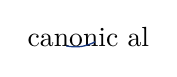
\begin{tikzpicture}[baseline=(word.base)]\node[inner sep=0pt] (word) {canonic al};\draw[color=blue,line width=.45pt] ([xshift=-.8em,yshift=.15ex]word.south) to[bend right=18] ([xshift=.25em,yshift=.5ex]word.south);\end{tikzpicture}}{canonical}{authorial word join}{ps_134-3_077-v0006} functor $a \hand{\mapsto} A_{/a}$ from $A= \hand{\Delta}^{f}$ to (Cat), which is the
ultimate choice for checking whether or not A is a test category, finally
gives the answer: it is not. Because with I now the Lawvere element, we
still have that $A_{/\hand{\Delta}_{o}\times I}$ is a two-point discrete category. Thus \var{\over[typed]{A}{t}}{t}{typewriter overwriting}{ps_134-3_077-v0007}he topos
$A^{\hand{\wedge}}= (\hand{\Delta}^{f})^{\hand{\wedge}}$ is'nt locally modelizing i.e. it has'nt got any homotopy \var{\xout{\unsure{seg}}}{}{typewriter deletion}{ps_134-3_077-v0008}\var{\inserted[typed]{in}}{in}{typed insertion}{ps_134-3_077-v0009}-%
\var{\xout{\unsure{ment}}}{}{typewriter deletion}{ps_134-3_077-v0010}\var{\inserted[typed]{terval}}{terval}{typed insertion}{ps_134-3_077-v0011}, which at any rate is a very big drawback I would think. The only
hope which still remains, to account for the positive features of face-%
complexes recalled above, is that $\hand{\Delta}^{f}$ is at the least a test category \uline{in}
\uline{the wide sense} \var{\inserted{[or \uline{weak} test category]}}{\hand{[or \uline{weak} test category]}}{insertion}{ps_134-3_077-v0012}, namely that for any category C with final element, the
category $i_A j_A(C) = A_{/j_A(C)}$( = category of all \var{\xout{objects}}{}{typewriter deletion}{ps_134-3_077-v0013} pairs (n,u)\var{\inserted{,}}{\hand{,}}{insertion}{ps_134-3_077-v0014} with
u a map of the (ordered\var{\over{)}{)}}{\hand{)}}{writing over}{ps_134-3_077-v0015} category $A_{/\tilde{\hand{\Delta}}_n}$ \var{\inserted{into C}}{\hand{into C}}{insertion}{ps_134-3_077-v0016}) is aspheric. The first case to
check is for C = final category $\hand{\Delta}_o$ , i.e. \var{\xout{asyclicity}}{}{typewriter deletion}{ps_134-3_077-v0017} asphericity of A ,
next step would be $C =\hand{\Delta}_1$ , i.e. asphericity of the Lawvere element $L_A$
(but of course \uline{not} asphericity over the final element $e_{A^{\hand{\wedge}}}$ \hand{!}).

The question certainly deserves to be settled. If the answer is
affirmative i.e. $\hand{\Delta}^{f}$ \uline{is} a test category in the wide sense, then\var{\xout{x}}{}{typewriter deletion}{ps_134-3_077-v0018} the proposi-%
\margin{-} tion stated earlier (\hand{\S}. \hand{42}), which clearly applies equally when A is a
test category in the wide sense, implies that if M is\var{\xout{x}}{}{typewriter deletion}{ps_134-3_077-v0019} any full subcatego-%
ry of (Cat) containing all those C which are ``locally isomorphic'' to $\hand{\Delta}^{f}$ ,
(i.e. such that for every $x \hand{\in} C$, $C_{/x}$ is isomorphic to the ordered category
of all subsimplices of some simplex), then for the induced notion $W_M$ of
weak equivalences, M is a modelizer and the inclusion functor from M into
(Cat) is modelizing. This does not yet apply to (Ord), however it reopens
the question whether the \var{\inserted{full sub}}{\hand{full sub}}{insertion}{ps_134-3_077-v0020}category of \var{\inserted{(Ord) made up by all}}{\hand{(Ord) made up by all}}{insertion}{ps_134-3_077-v0021} \var{\deleted{``simplicial maquettes'', which can be}}{}{deletion}{ps_134-3_077-v0022}
\var{\deleted{interpreted as}}{}{deletion}{ps_134-3_077-v0023} ordered sets J which are locally isomorphic to $\hand{\Delta}^{f}$ in the
sense above (namely for any $x \hand{\in} J$, the \var{\xout{subse}}{}{typewriter deletion}{ps_134-3_077-v0024} ordered subset $J_{\hand{\leq} x}$ is isomor-%

%% END SOURCE ps_134-3_077
\ifnum\EditionMode=1
\psapparatusstart
\psentry{ps_134-3_077-v0001}{1}{writing over}{$\over{f}{f}$}{$\hand{f}$}{The superposed handwritten reading replaces the underlying reading.}
\psentry{ps_134-3_077-v0002}{2}{writing over}{$\over{f}{f}$}{$\hand{f}$}{The superposed handwritten reading replaces the underlying reading.}
\psentry{ps_134-3_077-v0003}{3}{typed insertion}{\inserted[typed]{to look}}{to look}{The typed insertion is incorporated at its indicated position; insertion brackets leave the running text.}
\psentry{ps_134-3_077-v0004}{4}{writing over}{\over{n}{n}}{\hand{n}}{The superposed handwritten reading replaces the underlying reading.}
\psentry{ps_134-3_077-v0005}{5}{insertion}{\inserted{again}}{\hand{again}}{The handwritten insertion is incorporated at its indicated position; insertion brackets leave the running text.}
\psentry{ps_134-3_077-v0006}{6}{authorial word join}{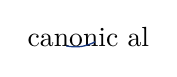
\begin{tikzpicture}[baseline=(word.base)]\node[inner sep=0pt] (word) {canonic al};\draw[color=blue,line width=.45pt] ([xshift=-.8em,yshift=.15ex]word.south) to[bend right=18] ([xshift=.25em,yshift=.5ex]word.south);\end{tikzpicture}}{canonical}{A pen joining curve closes the typed internal blank in canonic al.}
\psentry{ps_134-3_077-v0007}{7}{typewriter overwriting}{\over[typed]{A}{t}}{t}{The superposed typed reading replaces the underlying reading.}
\psentry{ps_134-3_077-v0008}{8}{typewriter deletion}{\xout{\unsure{seg}}}{}{The typewriter strikes out this material; it leaves the corrected running text.}
\psentry{ps_134-3_077-v0009}{9}{typed insertion}{\inserted[typed]{in}}{in}{The typed insertion is incorporated at its indicated position; insertion brackets leave the running text.}
\psentry{ps_134-3_077-v0010}{10}{typewriter deletion}{\xout{\unsure{ment}}}{}{The typewriter strikes out this material; it leaves the corrected running text.}
\psentry{ps_134-3_077-v0011}{11}{typed insertion}{\inserted[typed]{terval}}{terval}{The typed insertion is incorporated at its indicated position; insertion brackets leave the running text.}
\psentry{ps_134-3_077-v0012}{12}{insertion}{\inserted{[or \uline{weak} test category]}}{\hand{[or \uline{weak} test category]}}{The handwritten insertion is incorporated at its indicated position; insertion brackets leave the running text.}
\psentry{ps_134-3_077-v0013}{13}{typewriter deletion}{\xout{objects}}{}{The typewriter strikes out this material; it leaves the corrected running text.}
\psentry{ps_134-3_077-v0014}{14}{insertion}{\inserted{,}}{\hand{,}}{The handwritten insertion is incorporated at its indicated position; insertion brackets leave the running text.}
\psentry{ps_134-3_077-v0015}{15}{writing over}{\over{)}{)}}{\hand{)}}{The superposed handwritten reading replaces the underlying reading.}
\psentry{ps_134-3_077-v0016}{16}{insertion}{\inserted{into C}}{\hand{into C}}{The handwritten insertion is incorporated at its indicated position; insertion brackets leave the running text.}
\psentry{ps_134-3_077-v0017}{17}{typewriter deletion}{\xout{asyclicity}}{}{The typewriter strikes out this material; it leaves the corrected running text.}
\psentry{ps_134-3_077-v0018}{18}{typewriter deletion}{\xout{x}}{}{The typewriter strikes out this material; it leaves the corrected running text.}
\psentry{ps_134-3_077-v0019}{19}{typewriter deletion}{\xout{x}}{}{The typewriter strikes out this material; it leaves the corrected running text.}
\psentry{ps_134-3_077-v0020}{20}{insertion}{\inserted{full sub}}{\hand{full sub}}{The handwritten insertion is incorporated at its indicated position; insertion brackets leave the running text.}
\psentry{ps_134-3_077-v0021}{21}{insertion}{\inserted{(Ord) made up by all}}{\hand{(Ord) made up by all}}{The handwritten insertion is incorporated at its indicated position; insertion brackets leave the running text.}
\psentry{ps_134-3_077-v0022}{22}{deletion}{\deleted{``simplicial maquettes'', which can be}}{}{The author cancels this material by hand; it leaves the corrected running text.}
\psentry{ps_134-3_077-v0023}{23}{deletion}{\deleted{interpreted as}}{}{The author cancels this material by hand; it leaves the corrected running text.}
\psentry{ps_134-3_077-v0024}{24}{typewriter deletion}{\xout{subse}}{}{The typewriter strikes out this material; it leaves the corrected running text.}
\psapparatusend
\fi
\pssource{ps_134-3_078}{134-3/78}{https://grothendieck.umontpellier.fr/web/viewer.html?file=../134-3.pdf\#page=79}
\psnumber{ps_134-3_078-v0001}{1}
\psnumber{ps_134-3_078-v0002}{2}
\psnumber{ps_134-3_078-v0003}{3}
\psnumber{ps_134-3_078-v0004}{4}
\psnumber{ps_134-3_078-v0005}{5}
\psnumber{ps_134-3_078-v0006}{6}
\psnumber{ps_134-3_078-v0007}{7}
\psnumber{ps_134-3_078-v0008}{8}
\psnumber{ps_134-3_078-v0009}{9}
\psnumber{ps_134-3_078-v0010}{10}
\psnumber{ps_134-3_078-v0011}{11}
\psnumber{ps_134-3_078-v0012}{12}
\psnumber{ps_134-3_078-v0013}{13}
\psnumber{ps_134-3_078-v0014}{14}
\psnumber{ps_134-3_078-v0015}{15}
%% BEGIN SOURCE ps_134-3_078
% Pursuing Stacks (cotes 134-2 to 134-8): archive cote 134-3, site page 78 (PDF page 79), typescript page 78.
% typescript. Draft compared: ps2.tex:4036-4092.
% AI-transcribed by Claude Opus 5.5 (claude-opus-5-5, adaptive thinking, effort high), Message Batches API, batch ps1 (msgbatch_01Rv5hCaNTtUt4JHx1yqoHPL), 2026-11-12; image review recorded in records/CHECK_DECISIONS_134_3_4.tsv.
\scanpage{134-3/78}
\mspage{78}

phic to the ordered set of subsimplices of some simplex) is a modelizer.
To insure this,  it would be enough to find an ordered set J satisfying the
previous condition \var{\deleted{(namely a simplicial maquette)}}{}{deletion}{ps_134-3_078-v0001} \var{\inserted{(for instance one stemming from a ``simplicial maquette'')}}{\hand{(for instance one stemming from a ``simplicial maquette'')}}{insertion}{ps_134-3_078-v0002}, such that the correspon-%
ding category is a test category,  or at least a test category in the wide
sense.  The first candidate that comes to my mind,  is to take any \uline{infinite}
set S of vertices,  and take J to be the ordered set of all \uline{finite} \uline{non-emp\var{\over[typed]{t}{-}}{-}{typewriter overwriting}{ps_134-3_078-v0003}}%
\uline{ty} subsets (called the simplices  -  thus the elements of S can be inter-%
preted in terms of J as the minimal simplices).  By the way,  the category
associated to J,  in case S = $\underline{N}$ ,  can be interpreted in terms of \var{\inserted{$A=\Delta^f$}}{\hand{$A=\Delta^f$}}{insertion}{ps_134-3_078-v0004} as
the category  $A_{\hand{/\Delta}_{\mathrm{oo}}}$ ,  where \hand{\ensuremath{\Delta}}$_{\mathrm{oo}}$ is defined as the filtering direct limit
\var{\xout{of}}{}{typewriter deletion}{ps_134-3_078-v0005} in A\hand{\ensuremath{^{\wedge}}} of the \hand{\ensuremath{\Delta}}$_n$'s ,  arranged into a direct system in the obvious way:
\var{\xout{The As the category J admits binary products (namely intersection of simpli-}}{}{typewriter deletion}{ps_134-3_078-v0006}%
\var{\xout{ces}}{}{typewriter deletion}{ps_134-3_078-v0007}
\[ \hand{\ensuremath{\Delta}}_{\hand{\infty}} = \underset{n}{\underset{\hand{\ensuremath{\longrightarrow}}}{\mathrm{lim}}}\ \hand{\ensuremath{\Delta}}_n \quad \text{in} \quad (\hand{\ensuremath{\Delta}}^f)^{\hand{\wedge}}\ . \]
Asphericity of J looks intuitively evident,  and should be easy by a direct
limit argument,  as a matter of fact any filtering \var{\xout{\unsure{inex}}}{}{typewriter deletion}{ps_134-3_078-v0008} category (the next
best to having a final element) should be aspheric,  at least if it has a
countable cofinal family of objects.  T\var{\over[typed]{h}{h}}{h}{typewriter overwriting}{ps_134-3_078-v0009}e Lawvere element \var{\xout{in}}{}{typewriter deletion}{ps_134-3_078-v0010} L$_A$ in A\hand{\ensuremath{^{\wedge}}} is not
aspheric though over the final object,  because when inducing over a zero
simplex,  we get the same contradiction as before.  As a matter of fact,
I am getting aware I have been very silly and prejudiced not to see one
trivial common reason,  applicable to \hand{\ensuremath{\Delta}}$^f$ as to J , showing that they are
not test categories nor even local test categories:  namely the induced
categories A$_{/a}$ should be test categories too,  but among these there are
one-point categories (take a=\hand{\ensuremath{\Delta}}$_o$ ,  or a zero-simplex),  and such a catego-%
ry is \uline{not} a test category!

Still J may be a test category in the wide sense - the basic test here,
as we know already asphericity of \var{\over[typed]{I}{J}}{J}{typewriter overwriting}{ps_134-3_078-v0011} itself,  would be \var{\inserted[typed]{(absolute)}}{(absolute)}{typed insertion}{ps_134-3_078-v0012} asphericity of L$_J$ ,
or equivalently,  of the category J$_{/L_J}$ ,  an ordered set in fact, \var{\xout{of}}{}{typewriter deletion}{ps_134-3_078-v0013}
\var{\xout{all}}{}{typewriter deletion}{ps_134-3_078-v0014}(as is the case for any category A$_{/F}$ for A defined by an ordered set
and F in A\hand{\ensuremath{^{\wedge}}}).  This is now the ordered set of all pairs \var{\xout{(K)}}{}{typewriter deletion}{ps_134-3_078-v0015} (K\hand{\ensuremath{\subset}}T)  of
finite subsets of S,  with T in J namely T non empty,  with the rule
\[ (K',T') \hand{\ensuremath{\leqslant}} (K,T) \quad \text{iff} \quad T'\hand{\ensuremath{\subset}}T \ \text{and}\ K'=K\hand{\ensuremath{\cap}}T' \quad . \]

%% END SOURCE ps_134-3_078
\ifnum\EditionMode=1
\psapparatusstart
\psentry{ps_134-3_078-v0001}{1}{deletion}{\deleted{(namely a simplicial maquette)}}{}{The author cancels this material by hand; it leaves the corrected running text.}
\psentry{ps_134-3_078-v0002}{2}{insertion}{\inserted{(for instance one stemming from a ``simplicial maquette'')}}{\hand{(for instance one stemming from a ``simplicial maquette'')}}{The handwritten insertion is incorporated at its indicated position; insertion brackets leave the running text.}
\psentry{ps_134-3_078-v0003}{3}{typewriter overwriting}{\over[typed]{t}{-}}{-}{The superposed typed reading replaces the underlying reading.}
\psentry{ps_134-3_078-v0004}{4}{insertion}{\inserted{$A=\Delta^f$}}{\hand{$A=\Delta^f$}}{The handwritten insertion is incorporated at its indicated position; insertion brackets leave the running text.}
\psentry{ps_134-3_078-v0005}{5}{typewriter deletion}{\xout{of}}{}{The typewriter strikes out this material; it leaves the corrected running text.}
\psentry{ps_134-3_078-v0006}{6}{typewriter deletion}{\xout{The As the category J admits binary products (namely intersection of simpli-}}{}{The typewriter strikes out this material; it leaves the corrected running text.}
\psentry{ps_134-3_078-v0007}{7}{typewriter deletion}{\xout{ces}}{}{The typewriter strikes out this material; it leaves the corrected running text.}
\psentry{ps_134-3_078-v0008}{8}{typewriter deletion}{\xout{\unsure{inex}}}{}{The typewriter strikes out this material; it leaves the corrected running text.}
\psentry{ps_134-3_078-v0009}{9}{typewriter overwriting}{\over[typed]{h}{h}}{h}{The superposed typed reading replaces the underlying reading.}
\psentry{ps_134-3_078-v0010}{10}{typewriter deletion}{\xout{in}}{}{The typewriter strikes out this material; it leaves the corrected running text.}
\psentry{ps_134-3_078-v0011}{11}{typewriter overwriting}{\over[typed]{I}{J}}{J}{The superposed typed reading replaces the underlying reading.}
\psentry{ps_134-3_078-v0012}{12}{typed insertion}{\inserted[typed]{(absolute)}}{(absolute)}{The typed insertion is incorporated at its indicated position; insertion brackets leave the running text.}
\psentry{ps_134-3_078-v0013}{13}{typewriter deletion}{\xout{of}}{}{The typewriter strikes out this material; it leaves the corrected running text.}
\psentry{ps_134-3_078-v0014}{14}{typewriter deletion}{\xout{all}}{}{The typewriter strikes out this material; it leaves the corrected running text.}
\psentry{ps_134-3_078-v0015}{15}{typewriter deletion}{\xout{(K)}}{}{The typewriter strikes out this material; it leaves the corrected running text.}
\psapparatusend
\fi
\pssource{ps_134-3_079}{134-3/79}{https://grothendieck.umontpellier.fr/web/viewer.html?file=../134-3.pdf\#page=80}
\psnumber{ps_134-3_079-v0001}{1}
\psnumber{ps_134-3_079-v0002}{2}
\psnumber{ps_134-3_079-v0003}{3}
\psnumber{ps_134-3_079-v0004}{4}
\psnumber{ps_134-3_079-v0005}{5}
\psnumber{ps_134-3_079-v0006}{6}
\psnumber{ps_134-3_079-v0007}{7}
\psnumber{ps_134-3_079-v0008}{8}
\psnumber{ps_134-3_079-v0009}{9}
\psnumber{ps_134-3_079-v0010}{10}
\psnumber{ps_134-3_079-v0011}{11}
\psnumber{ps_134-3_079-v0012}{12}
\psnumber{ps_134-3_079-v0013}{13}
\psnumber{ps_134-3_079-v0014}{14}
\psnumber{ps_134-3_079-v0015}{15}
\psnumber{ps_134-3_079-v0016}{16}
\psnumber{ps_134-3_079-v0017}{17}
\psnumber{ps_134-3_079-v0018}{18}
\psnumber{ps_134-3_079-v0019}{19}
\psnumber{ps_134-3_079-v0020}{20}
\psnumber{ps_134-3_079-v0021}{21}
\psnumber{ps_134-3_079-v0022}{22}
\psnumber{ps_134-3_079-v0023}{23}
\psnumber{ps_134-3_079-v0024}{24}
\psnumber{ps_134-3_079-v0025}{25}
\psnumber{ps_134-3_079-v0026}{26}
\psnumber{ps_134-3_079-v0027}{27}
\psnumber{ps_134-3_079-v0028}{28}
%% BEGIN SOURCE ps_134-3_079
% Pursuing Stacks (cotes 134-2 to 134-8): archive cote 134-3, site page 79 (PDF page 80), typescript page 79.
% typescript. Draft compared: ps2.tex:4074-4163.
% AI-transcribed by Claude Opus 5.5 (claude-opus-5-5, adaptive thinking, effort high), Message Batches API, batch ps1 (msgbatch_01Rv5hCaNTtUt4JHx1yqoHPL), 2026-11-12; image review recorded in records/CHECK_DECISIONS_134_3_4.tsv.
\scanpage{134-3/79}
\mspage{79}

26.3.

44. I finally convinced myself that $\hand{\Delta}^{f}$ , the category of standar\var{\over{\unsure{t}}{d}}{\hand{d}}{writing over}{ps_134-3_079-v0001}
ordered simplices with face operations (and no degeneracies) \uline{is} a ``test
category in the wide sense'' after all - although definitely not a test
category, as was seen yesterday (\var{\deleted{as}}{}{deletion}{ps_134-3_079-v0002} \var{\inserted{turning out to be}}{\hand{turning out to be}}{insertion}{ps_134-3_079-v0003} a practically trivial observation).
This now does rehabilitate the notion of a test category in the wide sense\hand{,}
which I expected to be of little or no interest - \var{\inserted{much the \deleted{same} way}}{\hand{much the  way}}{insertion}{ps_134-3_079-v0004} as previously, the
notion I now call by the name ``test category'' was rehabilitated or rather,
discovered, after I expected that the only one proper notion for getting
modelizers of the f\var{\over{\unsure{ro}}{or}}{\hand{or}}{writing over}{ps_134-3_079-v0005}m $A^{\hand{\wedge}}$ was in terms of conditions T 1) to T 3) on $A$.
\hand{(}including the very strong condition T 2) of total a\var{\over{\unsure{cycli}}{spheri}}{\hand{spheri}}{writing over}{ps_134-3_079-v0006}city\hand{)}. This notion
I \var{\inserted{then}}{\hand{then}}{insertion}{ps_134-3_079-v0007} finally called by the name``\uline{strict} test category'', and I was fortunately
cautious enough to reserve a name too for the notion which appeared then
as rather weak and \var{\xout{and}}{}{typewriter deletion}{ps_134-3_079-v0008} unmanageable, of test categories in the wide sense
or, as I will say \var{\inserted{now}}{\hand{now}}{insertion}{ps_134-3_079-v0009} more shortly, \uline{weak} \uline{test} \uline{categories} (by which of cour-%
se I do not mean to exclude the possibility that \hand{\unsure{it}} \unsure{some} \var{\inserted{be}}{\hand{be}}{insertion}{ps_134-3_079-v0010} even \hand{a} test catego-%
r\var{\over{\unsure{ies}}{y}}{\hand{y}}{writing over}{ps_134-3_079-v0011}\hand{)}, thus getting the trilogy of \var{\inserted[typed]{notions with}}{notions with}{typed insertion}{ps_134-3_079-v0012} strict implications
\[ \text{weak test categor\var{\over[typed]{y}{i}}{i}{typewriter overwriting}{ps_134-3_079-v0013}es} \hand{\Leftarrow} \text{test categor\var{\over[typed]{\unsure{m}}{i}}{i}{typewriter overwriting}{ps_134-3_079-v0014}es} \hand{\Leftarrow} \text{strict test categories} \quad . \]
In order not to get confused, I will recall what exactly each of these
notions means,

a) \var{\inserted[typed]{\uline{Weak}}}{\uline{Weak}}{typed insertion}{ps_134-3_079-v0015} \uline{\var{\over{T}{t}}{\hand{t}}{writing over}{ps_134-3_079-v0016}est categories}. \var{\xout{The category A is a}}{}{typewriter deletion}{ps_134-3_079-v0017} For a given \var{\inserted[typed]{small}}{small}{typed insertion}{ps_134-3_079-v0018} category $A$,
we look at the functor
\[ (1) \qquad i_A\colon A^{\hand{\wedge}} \hand{\longrightarrow} (\mathrm{Cat}) , \qquad \var{\over{F}{F}}{\hand{F}}{writing over}{ps_134-3_079-v0019} \hand{\longmapsto} A_{/F} \hand{,} \]
which commutes with direct limits, and at the right adjoint functor
\[ (2) \qquad j_A = i_A^{\var{\over[typed]{*}{*}}{*}{typewriter overwriting}{ps_134-3_079-v0020}} : \ (\mathrm{Cat}) \hand{\longrightarrow} A^{\hand{\wedge}}, \qquad C \hand{\longmapsto} \var{\over{j}{j}}{\hand{j}}{writing over}{ps_134-3_079-v0021}_A(C) = (a \hand{\mapsto} \mathrm{Hom}(A_{/a},C)) \ . \]
We get an adjunction \var{\xout{functor}}{}{typewriter deletion}{ps_134-3_079-v0022} morphism
\[ (3) \qquad i_A j_A(C) \hand{\longrightarrow} C \qquad \text{in } (\mathrm{Cat}) , \]
and another
\[ (4) \qquad F \hand{\longrightarrow} j_A i_A F \qquad \text{in } A^{\hand{\wedge}} , \]
functorial in $C$ resp. in $F$. Pr\var{\over{\illegible{1}}{es}}{\hand{es}}{writing over}{ps_134-3_079-v0023}umably the following are equivalent
(I'll see in a minute how much I can prove about these equivalences):

(i) T\var{\over[typed]{h}{h}}{h}{typewriter overwriting}{ps_134-3_079-v0024}e functors (1) and (2) are compatible with weak equivalences,
and the two \var{\inserted{induced}}{\hand{induced}}{insertion}{ps_134-3_079-v0025} functors between the localized categories
\[ \hand{(5)} \qquad W_A^{\hand{-1}} A^{\hand{\wedge}} \hand{\rightleftarrows} W^{-1}(\mathrm{Cat}) \overset{\mathrm{def}}{=} (\mathrm{Hot}) \ . \]
are equivalences.

(ii) As in (i), and moreover the two equivalences are quasi-inverse of
each other, with adjunction morphism\var{\deleted{s}}{}{deletion}{ps_134-3_079-v0026} \var{\over[typed]{o}{i}}{i}{typewriter overwriting}{ps_134-3_079-v0027}n \var{\deleted{(Cat}}{}{deletion}{ps_134-3_079-v0028} $W^{-1}(\mathrm{Cat}) = (\mathrm{Hot})$
deduced from (3) by localization.

\margin{\textcolor{black}{\unsure{(i}}}

%% END SOURCE ps_134-3_079
\ifnum\EditionMode=1
\psapparatusstart
\psentry{ps_134-3_079-v0001}{1}{writing over}{\over{\unsure{t}}{d}}{\hand{d}}{The superposed handwritten reading replaces the underlying reading.}
\psentry{ps_134-3_079-v0002}{2}{deletion}{\deleted{as}}{}{The author cancels this material by hand; it leaves the corrected running text.}
\psentry{ps_134-3_079-v0003}{3}{insertion}{\inserted{turning out to be}}{\hand{turning out to be}}{The handwritten insertion is incorporated at its indicated position; insertion brackets leave the running text.}
\psentry{ps_134-3_079-v0004}{4}{insertion}{\inserted{much the \deleted{same} way}}{\hand{much the  way}}{The handwritten insertion is incorporated at its indicated position; insertion brackets leave the running text.}
\psentry{ps_134-3_079-v0005}{5}{writing over}{\over{\unsure{ro}}{or}}{\hand{or}}{The superposed handwritten reading replaces the underlying reading.}
\psentry{ps_134-3_079-v0006}{6}{writing over}{\over{\unsure{cycli}}{spheri}}{\hand{spheri}}{The superposed handwritten reading replaces the underlying reading.}
\psentry{ps_134-3_079-v0007}{7}{insertion}{\inserted{then}}{\hand{then}}{The handwritten insertion is incorporated at its indicated position; insertion brackets leave the running text.}
\psentry{ps_134-3_079-v0008}{8}{typewriter deletion}{\xout{and}}{}{The typewriter strikes out this material; it leaves the corrected running text.}
\psentry{ps_134-3_079-v0009}{9}{insertion}{\inserted{now}}{\hand{now}}{The handwritten insertion is incorporated at its indicated position; insertion brackets leave the running text.}
\psentry{ps_134-3_079-v0010}{10}{insertion}{\inserted{be}}{\hand{be}}{The handwritten insertion is incorporated at its indicated position; insertion brackets leave the running text.}
\psentry{ps_134-3_079-v0011}{11}{writing over}{\over{\unsure{ies}}{y}}{\hand{y}}{The superposed handwritten reading replaces the underlying reading.}
\psentry{ps_134-3_079-v0012}{12}{typed insertion}{\inserted[typed]{notions with}}{notions with}{The typed insertion is incorporated at its indicated position; insertion brackets leave the running text.}
\psentry{ps_134-3_079-v0013}{13}{typewriter overwriting}{\over[typed]{y}{i}}{i}{The superposed typed reading replaces the underlying reading.}
\psentry{ps_134-3_079-v0014}{14}{typewriter overwriting}{\over[typed]{\unsure{m}}{i}}{i}{The superposed typed reading replaces the underlying reading.}
\psentry{ps_134-3_079-v0015}{15}{typed insertion}{\inserted[typed]{\uline{Weak}}}{\uline{Weak}}{The typed insertion is incorporated at its indicated position; insertion brackets leave the running text.}
\psentry{ps_134-3_079-v0016}{16}{writing over}{\over{T}{t}}{\hand{t}}{The superposed handwritten reading replaces the underlying reading.}
\psentry{ps_134-3_079-v0017}{17}{typewriter deletion}{\xout{The category A is a}}{}{The typewriter strikes out this material; it leaves the corrected running text.}
\psentry{ps_134-3_079-v0018}{18}{typed insertion}{\inserted[typed]{small}}{small}{The typed insertion is incorporated at its indicated position; insertion brackets leave the running text.}
\psentry{ps_134-3_079-v0019}{19}{writing over}{$\over{F}{F}$}{$\hand{F}$}{The superposed handwritten reading replaces the underlying reading.}
\psentry{ps_134-3_079-v0020}{20}{typewriter overwriting}{$\over[typed]{*}{*}$}{$*$}{The superposed typed reading replaces the underlying reading.}
\psentry{ps_134-3_079-v0021}{21}{writing over}{$\over{j}{j}$}{$\hand{j}$}{The superposed handwritten reading replaces the underlying reading.}
\psentry{ps_134-3_079-v0022}{22}{typewriter deletion}{\xout{functor}}{}{The typewriter strikes out this material; it leaves the corrected running text.}
\psentry{ps_134-3_079-v0023}{23}{writing over}{\over{\illegible{1}}{es}}{\hand{es}}{The superposed handwritten reading replaces the underlying reading.}
\psentry{ps_134-3_079-v0024}{24}{typewriter overwriting}{\over[typed]{h}{h}}{h}{The superposed typed reading replaces the underlying reading.}
\psentry{ps_134-3_079-v0025}{25}{insertion}{\inserted{induced}}{\hand{induced}}{The handwritten insertion is incorporated at its indicated position; insertion brackets leave the running text.}
\psentry{ps_134-3_079-v0026}{26}{deletion}{\deleted{s}}{}{The author cancels this material by hand; it leaves the corrected running text.}
\psentry{ps_134-3_079-v0027}{27}{typewriter overwriting}{\over[typed]{o}{i}}{i}{The superposed typed reading replaces the underlying reading.}
\psentry{ps_134-3_079-v0028}{28}{deletion}{\deleted{(Cat}}{}{The author cancels this material by hand; it leaves the corrected running text.}
\psapparatusend
\fi
\pssource{ps_134-3_080}{134-3/80}{https://grothendieck.umontpellier.fr/web/viewer.html?file=../134-3.pdf\#page=81}
\psnumber{ps_134-3_080-v0001}{1}
\psnumber{ps_134-3_080-v0002}{2}
\psnumber{ps_134-3_080-v0003}{3}
\psnumber{ps_134-3_080-v0004}{4}
\psnumber{ps_134-3_080-v0005}{5}
\psnumber{ps_134-3_080-v0006}{6}
\psnumber{ps_134-3_080-v0007}{7}
\psnumber{ps_134-3_080-v0008}{8}
\psnumber{ps_134-3_080-v0009}{9}
\psnumber{ps_134-3_080-v0010}{10}
\psnumber{ps_134-3_080-v0011}{11}
\psnumber{ps_134-3_080-v0012}{12}
\psnumber{ps_134-3_080-v0013}{13}
\psnumber{ps_134-3_080-v0014}{14}
\psnumber{ps_134-3_080-v0015}{15}
\psnumber{ps_134-3_080-v0016}{16}
\psnumber{ps_134-3_080-v0017}{17}
\psnumber{ps_134-3_080-v0018}{18}
\psnumber{ps_134-3_080-v0019}{19}
\psnumber{ps_134-3_080-v0020}{20}
\psnumber{ps_134-3_080-v0021}{21}
\psnumber{ps_134-3_080-v0022}{22}
\psnumber{ps_134-3_080-v0023}{23}
\psnumber{ps_134-3_080-v0024}{24}
\psnumber{ps_134-3_080-v0025}{25}
\psnumber{ps_134-3_080-v0026}{26}
\psnumber{ps_134-3_080-v0027}{27}
\psnumber{ps_134-3_080-v0028}{28}
\psnumber{ps_134-3_080-v0029}{29}
\psnumber{ps_134-3_080-v0030}{30}
\psnumber{ps_134-3_080-v0031}{31}
%% BEGIN SOURCE ps_134-3_080
% Pursuing Stacks (cotes 134-2 to 134-8): archive cote 134-3, site page 80 (PDF page 81), typescript page 80.
% typescript. Draft compared: ps2.tex:4144-4223.
% AI-transcribed by Claude Opus 5.5 (claude-opus-5-5, adaptive thinking, effort high), Message Batches API, batch ps1 (msgbatch_01Rv5hCaNTtUt4JHx1yqoHPL), 2026-11-12; image review recorded in records/CHECK_DECISIONS_134_3_4.tsv.
\scanpage{134-3/80}
\mspage{(80)}

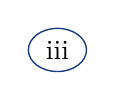
\begin{tikzpicture}[baseline=(n.base)]\node[inner sep=0pt] (n) {iii};\draw[color=blue,line width=.5pt] (n.center) ellipse [x radius=1.05em,y radius=.78em];\end{tikzpicture} As in (ii), but moreover the adjunction morphism in $W_A^{\hand{-1}}A^{\hand{\wedge}}$ for
the pair of quasi-inverse equivalences \var{\inserted[typed]{(5)}}{(5)}{typed insertion}{ps_134-3_080-v0001}, being \hand{likewise deduced from }\var{\inserted{(4).}}{\hand{(4).}}{insertion}{ps_134-3_080-v0002}
(iv) For any C in (Cat), (3) is a weak equivalence.
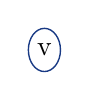
\begin{tikzpicture}[baseline=(n.base)]\node[inner sep=0pt] (n) {v};\draw[color=blue,line width=.5pt] (n.center) ellipse [x radius=.58em,y radius=.78em];\end{tikzpicture} Same as (iv), with C restricted to having a final element, i.e.
for any such C, $j_Ai_A(C) = A_{/j_A(C)}$ is a\var{\over{\unsure{s}}{s}}{\hand{s}}{writing over}{ps_134-3_080-v0003}pheric.
(vi) For any F in $A^{\hand{\wedge}}$, (4) is a weak equivalence, moreover
\[ W_{(Cat)} = j_A^{-1}(W_A) \qquad , \]
i.e. a \var{\xout{functor}}{}{typewriter deletion}{ps_134-3_080-v0004} map $f\colon C' \hand{\to} C$ in (Cat) is a \var{\xout{quasi}}{}{typewriter deletion}{ps_134-3_080-v0005} \var{\inserted[typed]{weak}}{weak}{typed insertion}{ps_134-3_080-v0006} equivalence,
iff $j_A(f)$ is a \var{\xout{quasi}}{}{typewriter deletion}{ps_134-3_080-v0007} \var{\inserted[typed]{weak}}{weak}{typed insertion}{ps_134-3_080-v0008} equivalence in $A^{\hand{\wedge}}$ - which means, by defi-%
n\var{\over[typed]{\illegible{1}}{i}}{i}{typewriter overwriting}{ps_134-3_080-v0009}tion (more or less) that $i_Aj_A(f)$ is a \var{\xout{quasi}}{}{typewriter deletion}{ps_134-3_080-v0010} \var{\inserted[typed]{weak}}{weak}{typed insertion}{ps_134-3_080-v0011} equivalence.
(vii) T\var{\over{h}{h}}{\hand{h}}{writing over}{ps_134-3_080-v0012}e functor
(6) \[ i_Aj_A \; : \; (Cat) \hand{\longrightarrow} (Cat) \quad , \quad C \hand{\mapsto} A_{/j_A(C)} \, , \]
transforms \var{\xout{quasi}}{}{typewriter deletion}{ps_134-3_080-v0013} \var{\inserted[typed]{weak}}{weak}{typed insertion}{ps_134-3_080-v0014} equivalences into \var{\xout{quasi}}{}{typewriter deletion}{ps_134-3_080-v0015} \var{\inserted[typed]{weak}}{weak}{typed insertion}{ps_134-3_080-v0016} equivalences , i.e.
gives rise to a functor (Hot)$\hand{\to}$(Hot), and moreover \var{\deleted{A is}}{}{deletion}{ps_134-3_080-v0017} \hand{the}
\var{\deleted{aspheric.}}{}{deletion}{ps_134-3_080-v0018} \hand{latter respects final object (i.e. A is aspheric).}
(viii) Same as (vii), but restricting to \var{\xout{quax}}{}{typewriter deletion}{ps_134-3_080-v0019} weak equivalences of the
type $C \hand{\to} \var{\over[typed]{e}{e}}{e}{typewriter overwriting}{ps_134-3_080-v0020}$, where C has a final element and e is the final
object in (Cat) (the one-point category)\hand{, plus asphericity of A.}

The trivial implications between all these conditions can be summari\var{\xout{z}}{}{typewriter deletion}{ps_134-3_080-v0021}
zed in the diagram
% Hand-drawn arrows are marked blue; typed objects remain plain.
\diagram{\begin{tikzcd}[row sep=small, arrows=Rightarrow]
(iii) \ar[r,Leftrightarrow,color=blue] \ar[d,color=blue] \& (vi) \ar[r,color=blue] \& (vii) \ar[r,color=blue] \& (viii) \ar[dl,color=blue] \\
(ii) \ar[r,color=blue] \ar[d,color=blue] \& (iv) \ar[r,color=blue] \& (v) \& \\
(i) \& , \& \&
\end{tikzcd}}
the only \var{\inserted[typed]{slightly}}{slightly}{typed insertion}{ps_134-3_080-v0022} less obvious implication here is (viii)\hand{$\Rightarrow$}(v), which is seen
by looking at the commutative square deduced from $C \hand{\to} e$ (C in (Cat) as in
(v)\var{\xout{\unsure{;}}}{}{typewriter deletion}{ps_134-3_080-v0023} namely with final element) by applying (3)
\diagram{\begin{tikzcd}
i_Aj_A(C) \ar[r,color=blue] \ar[d,color=blue] \& C \ar[d,color=blue] \\
A{=}i_Aj_A(e) \ar[r,color=blue] \& e
\end{tikzcd} \quad ,}
by assumption the vertical arrows are weak equivalences, and so is $A \hand{\to} e$
(because A is supposed to be aspheric), therefore the same holds for the
fourth arrow left. On the other hand an easy asphericity argument
showed us \var{\inserted{[\unsure{\S}.30]}}{\hand{[\unsure{\S}.30]}}{insertion}{ps_134-3_080-v0024} that (v) \hand{$\Longrightarrow$}(iii), hence all conditions (ii) to (viii) are
equivalent, and they are equivalent to the stronger form of (iv), \var{\xout{that}}{}{typewriter deletion}{ps_134-3_080-v0025}
say (iv'), \var{\over[typed]{d}{s}}{s}{typewriter overwriting}{ps_134-3_080-v0026}\var{\over[typed]{a}{a}}{a}{typewriter overwriting}{ps_134-3_080-v0027}ying that (3) is \uline{aspheric} for any C in (Cat). T\var{\over{h}{h}}{\hand{h}}{writing over}{ps_134-3_080-v0028}e only
equivalence which is not quite clear yet is that (i) implies the other
conditions\unsure{\var{\over{,}{.}}{\hand{.}}{writing over}{ps_134-3_080-v0029}} \var{\deleted{under the formally weakest form (v) let's say.}}{}{deletion}{ps_134-3_080-v0030} B\var{\over{u}{u}}{\hand{u}}{writing over}{ps_134-3_080-v0031}t it is so

%% END SOURCE ps_134-3_080
\ifnum\EditionMode=1
\psapparatusstart
\psentry{ps_134-3_080-v0001}{1}{typed insertion}{\inserted[typed]{(5)}}{(5)}{The typed insertion is incorporated at its indicated position; insertion brackets leave the running text.}
\psentry{ps_134-3_080-v0002}{2}{insertion}{\inserted{(4).}}{\hand{(4).}}{The handwritten insertion is incorporated at its indicated position; insertion brackets leave the running text.}
\psentry{ps_134-3_080-v0003}{3}{writing over}{\over{\unsure{s}}{s}}{\hand{s}}{The superposed handwritten reading replaces the underlying reading.}
\psentry{ps_134-3_080-v0004}{4}{typewriter deletion}{\xout{functor}}{}{The typewriter strikes out this material; it leaves the corrected running text.}
\psentry{ps_134-3_080-v0005}{5}{typewriter deletion}{\xout{quasi}}{}{The typewriter strikes out this material; it leaves the corrected running text.}
\psentry{ps_134-3_080-v0006}{6}{typed insertion}{\inserted[typed]{weak}}{weak}{The typed insertion is incorporated at its indicated position; insertion brackets leave the running text.}
\psentry{ps_134-3_080-v0007}{7}{typewriter deletion}{\xout{quasi}}{}{The typewriter strikes out this material; it leaves the corrected running text.}
\psentry{ps_134-3_080-v0008}{8}{typed insertion}{\inserted[typed]{weak}}{weak}{The typed insertion is incorporated at its indicated position; insertion brackets leave the running text.}
\psentry{ps_134-3_080-v0009}{9}{typewriter overwriting}{\over[typed]{\illegible{1}}{i}}{i}{The superposed typed reading replaces the underlying reading.}
\psentry{ps_134-3_080-v0010}{10}{typewriter deletion}{\xout{quasi}}{}{The typewriter strikes out this material; it leaves the corrected running text.}
\psentry{ps_134-3_080-v0011}{11}{typed insertion}{\inserted[typed]{weak}}{weak}{The typed insertion is incorporated at its indicated position; insertion brackets leave the running text.}
\psentry{ps_134-3_080-v0012}{12}{writing over}{\over{h}{h}}{\hand{h}}{The superposed handwritten reading replaces the underlying reading.}
\psentry{ps_134-3_080-v0013}{13}{typewriter deletion}{\xout{quasi}}{}{The typewriter strikes out this material; it leaves the corrected running text.}
\psentry{ps_134-3_080-v0014}{14}{typed insertion}{\inserted[typed]{weak}}{weak}{The typed insertion is incorporated at its indicated position; insertion brackets leave the running text.}
\psentry{ps_134-3_080-v0015}{15}{typewriter deletion}{\xout{quasi}}{}{The typewriter strikes out this material; it leaves the corrected running text.}
\psentry{ps_134-3_080-v0016}{16}{typed insertion}{\inserted[typed]{weak}}{weak}{The typed insertion is incorporated at its indicated position; insertion brackets leave the running text.}
\psentry{ps_134-3_080-v0017}{17}{deletion}{\deleted{A is}}{}{The author cancels this material by hand; it leaves the corrected running text.}
\psentry{ps_134-3_080-v0018}{18}{deletion}{\deleted{aspheric.}}{}{The author cancels this material by hand; it leaves the corrected running text.}
\psentry{ps_134-3_080-v0019}{19}{typewriter deletion}{\xout{quax}}{}{The typewriter strikes out this material; it leaves the corrected running text.}
\psentry{ps_134-3_080-v0020}{20}{typewriter overwriting}{$\over[typed]{e}{e}$}{$e$}{The superposed typed reading replaces the underlying reading.}
\psentry{ps_134-3_080-v0021}{21}{typewriter deletion}{\xout{z}}{}{The typewriter strikes out this material; it leaves the corrected running text.}
\psentry{ps_134-3_080-v0022}{22}{typed insertion}{\inserted[typed]{slightly}}{slightly}{The typed insertion is incorporated at its indicated position; insertion brackets leave the running text.}
\psentry{ps_134-3_080-v0023}{23}{typewriter deletion}{\xout{\unsure{;}}}{}{The typewriter strikes out this material; it leaves the corrected running text.}
\psentry{ps_134-3_080-v0024}{24}{insertion}{\inserted{[\unsure{\S}.30]}}{\hand{[\unsure{\S}.30]}}{The handwritten insertion is incorporated at its indicated position; insertion brackets leave the running text.}
\psentry{ps_134-3_080-v0025}{25}{typewriter deletion}{\xout{that}}{}{The typewriter strikes out this material; it leaves the corrected running text.}
\psentry{ps_134-3_080-v0026}{26}{typewriter overwriting}{\over[typed]{d}{s}}{s}{The superposed typed reading replaces the underlying reading.}
\psentry{ps_134-3_080-v0027}{27}{typewriter overwriting}{\over[typed]{a}{a}}{a}{The superposed typed reading replaces the underlying reading.}
\psentry{ps_134-3_080-v0028}{28}{writing over}{\over{h}{h}}{\hand{h}}{The superposed handwritten reading replaces the underlying reading.}
\psentry{ps_134-3_080-v0029}{29}{writing over}{\over{,}{.}}{\hand{.}}{The superposed handwritten reading replaces the underlying reading.}
\psentry{ps_134-3_080-v0030}{30}{deletion}{\deleted{under the formally weakest form (v) let's say.}}{}{The author cancels this material by hand; it leaves the corrected running text.}
\psentry{ps_134-3_080-v0031}{31}{writing over}{\over{u}{u}}{\hand{u}}{The superposed handwritten reading replaces the underlying reading.}
\psapparatusend
\fi
\pssource{ps_134-3_081}{134-3/81}{https://grothendieck.umontpellier.fr/web/viewer.html?file=../134-3.pdf\#page=82}
\psnumber{ps_134-3_081-v0001}{1}
\psnumber{ps_134-3_081-v0002}{2}
\psnumber{ps_134-3_081-v0003}{3}
\psnumber{ps_134-3_081-v0004}{4}
\psnumber{ps_134-3_081-v0005}{5}
\psnumber{ps_134-3_081-v0006}{6}
\psnumber{ps_134-3_081-v0007}{7}
\psnumber{ps_134-3_081-v0008}{8}
\psnumber{ps_134-3_081-v0009}{9}
\psnumber{ps_134-3_081-v0010}{10}
\psnumber{ps_134-3_081-v0011}{11}
\psnumber{ps_134-3_081-v0012}{12}
\psnumber{ps_134-3_081-v0013}{13}
\psnumber{ps_134-3_081-v0014}{14}
\psnumber{ps_134-3_081-v0015}{15}
\psnumber{ps_134-3_081-v0016}{16}
\psnumber{ps_134-3_081-v0017}{17}
\psnumber{ps_134-3_081-v0018}{18}
\psnumber{ps_134-3_081-v0019}{19}
\psnumber{ps_134-3_081-v0020}{20}
\psnumber{ps_134-3_081-v0021}{21}
\psnumber{ps_134-3_081-v0022}{22}
\psnumber{ps_134-3_081-v0023}{23}
\psnumber{ps_134-3_081-v0024}{24}
\psnumber{ps_134-3_081-v0025}{25}
\psnumber{ps_134-3_081-v0026}{26}
\psnumber{ps_134-3_081-v0027}{27}
\psnumber{ps_134-3_081-v0028}{28}
\psnumber{ps_134-3_081-v0029}{29}
\psnumber{ps_134-3_081-v0030}{30}
\psnumber{ps_134-3_081-v0031}{31}
\psnumber{ps_134-3_081-v0032}{32}
%% BEGIN SOURCE ps_134-3_081
% Pursuing Stacks (cotes 134-2 to 134-8): archive cote 134-3, site page 81 (PDF page 82), typescript page 81.
% typescript. Draft compared: ps2.tex:4210-4279.
% AI-transcribed by Claude Opus 5.5 (claude-opus-5-5, adaptive thinking, effort high), Message Batches API, batch pilot (msgbatch_0189Nhf1xB615YWnztubtLfc), 2026-11-12; image review recorded in records/CHECK_DECISIONS_134_3_4.tsv.
\scanpage{134-3/81}
\mspage{81}

if we grant the ``insp\var{\xout{\unsure{i}}}{}{typewriter deletion}{ps_134-3_081-v0001}iring assumption'',\var{\xout{th}}{}{typewriter deletion}{ps_134-3_081-v0002} implying that any autoequivalen\var{\xout{x}}{}{typewriter deletion}{ps_134-3_081-v0003}
ce of(Hot)  is isomorphic to the identity functor  -  in this case it is
clear that even the weaker form (i')  of (i),  demanding only that
$i_Aj_A$ \var{\inserted{induce}}{\hand{induce}}{insertion}{ps_134-3_081-v0004} \var{\deleted{be}}{}{deletion}{ps_134-3_081-v0005} an \var{\inserted{auto}}{\hand{auto}}{insertion}{ps_134-3_081-v0006}equivalence \var{\inserted{of (Hot)}}{\hand{of (Hot)}}{insertion}{ps_134-3_081-v0007} (and \var{\inserted[typed]{nothing on}}{nothing on}{typed insertion}{ps_134-3_081-v0008} \var{\xout{\unsure{nothing}}}{}{typewriter deletion}{ps_134-3_081-v0009} either factor $i_A$ , $j_A$ \var{\inserted[typed]{in (5)}}{in (5)}{typed insertion}{ps_134-3_081-v0010}),implies (v).
Also,  When we assume moreover A aspheric,\var{\xout{\illegible{7}}}{}{typewriter deletion}{ps_134-3_081-v0011} it is clear that (i)
(and even (i')) implies (vii) i.e. all other conditions.  Thus,  instead \var{\xout{x}}{}{typewriter deletion}{ps_134-3_081-v0012}
of the assumption  on (Hot),  it would be enough to know that the particu-%
lar autoequivalence \var{\xout{$i_Aj_A$}}{}{typewriter deletion}{ps_134-3_081-v0013} of (Hot) induced by $i_Aj_A$  transforms the final
element of (Hot)  (respresented by the element e of (Cat)) into an isomor-%
phic one,\var{\inserted{\over{\unsure{(*)}}{(48)}}}{\hand{\hand{(48)}}}{insertion}{ps_134-3_081-v0014} which looks like a very slight strenghtening of (i) indeed.
\margin{\unsure{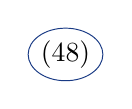
\begin{tikzpicture}[baseline=(n.base)]\node[inner sep=0pt] (n) {(48)};\draw[color=blue,line width=.35pt] (n.center) ellipse [x radius=1.35em,y radius=.95em];\end{tikzpicture} * 27.3. But this is true for any equivalence of categories -- I'm really being very dull!}}

In any case,  the conditions (ii) to (viii) are equivalent,  and
equivalent to  (i)  (or (i'))  \uline{plus} \var{\inserted{\over{\unsure{(**)}}{(49)}}}{\hand{\hand{(49)}}}{insertion}{ps_134-3_081-v0015} asphericity of A.  The formally
\margin{\unsure{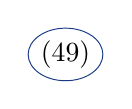
\begin{tikzpicture}[baseline=(n.base)]\node[inner sep=0pt] (n) {(49)};\draw[color=blue,line width=.35pt] (n.center) ellipse [x radius=1.35em,y radius=.95em];\end{tikzpicture} ** The ``plus'' is unnecessary visibly, see note above.}}
strongest form is (iii),  the formally weakest one (with the exception
of (i) or (i')\hand{)} \var{\deleted{plus \hand{(**)} asphericity of A)}}{}{deletion}{ps_134-3_081-v0016} is (v),  which is also the one
which looks the most concrete,  namely amenable to practical verification.
This was indeed what at the very beginning was attractive in this conditi-%
on,  in comparison to the first one that came to my mind when introducing
the notion of a modelizer and of model preserving functors  -  namely \var{\xout{that}}{}{typewriter deletion}{ps_134-3_081-v0017}
merely that  $i_A$  should induce an equivalence between the localized cate-%
gories,  or equivalently,  that $A^{\hand{\wedge}}$ should be a ``modelizer'' and $i_A$ should
be model-preserving.  That we should be more demanding and ask for $j_A$ to
be equally model preserving crept in first rather timidly  -  and I still
dont know (and didn\hand{'}t really stop to think)  if \var{\inserted{the first}}{\hand{the first}}{insertion}{ps_134-3_081-v0018} one implies the other\var{\deleted{(***)}}{}{deletion}{ps_134-3_081-v0019}\hand{(50)}.
\var{\margin{(***) In fact, it is the condition that $j_A = i_A^*$ \deleted{\illegible{1}}, \unsure{not $i_A$}, should be model preserving, which is ``the right'' condition on A, equivalent to A being a weak test category, \deleted{cf p.\unsure{88 remark 3.}} if A is assumed aspheric.}}{\margin{(***) In fact, it is the condition that $j_A = i_A^*$ , \unsure{not $i_A$}, should be model preserving, which is ``the right'' condition on A, equivalent to A being a weak test category,  if A is assumed aspheric.}}{marginal note revised}{ps_134-3_081-v0020}

In any case,  as far as checking a property goes,  I would consider
(v) to be \uline{the} handy definition of a weak test category,  whereas (iii)
is the best,  when it goes to making use of the fact that A i\var{\xout{s}}{}{typewriter deletion}{ps_134-3_081-v0021}s indeed a
weak test category.  As for (i),  \var{\deleted{(supplemented by asphericity to be safe)}}{}{deletion}{ps_134-3_081-v0022}
it corresponds to the main intuitive content of the notion,  which means
that homotopy types can be``modelled'' by elements of $A^{\hand{\wedge}}$ \var{\xout{using \unsure{$i_A$}}}{}{typewriter deletion}{ps_134-3_081-v0023} ,  using
$i_A$ for describing which homotopy type is describe\var{\xout{e}}{}{typewriter deletion}{ps_134-3_081-v0024}d by an element F of $A^{\hand{\wedge}}$,
and using $j_A$ for getting a model in $A^{\hand{\wedge}}$ for a given homotopy type, descri-%
be\var{\xout{e}}{}{typewriter deletion}{ps_134-3_081-v0025}d by an object C in (Cat).

b)  \var{\inserted{\deleted{\uline{Weak}}}}{\hand{}}{insertion}{ps_134-3_081-v0026} \uline{Test categories} \var{\inserted{and local test categories}}{\hand{and local test categories}}{insertion}{ps_134-3_081-v0027}.  Let A still be a small category.  T\var{\over[typed]{h}{h}}{h}{typewriter overwriting}{ps_134-3_081-v0028}en the follo-%
wing conditions are equivalent:

\var{\deleted{i)  A is a weak test category,  and so are all induced categories}}{}{deletion}{ps_134-3_081-v0029}
\var{\deleted{$A_{/a}$  with a in A.}}{}{deletion}{ps_134-3_081-v0030}
\var{\deleted{ii)  A is aspheric,  and for any aspheric element F in $A^{\hand{\wedge}}$, $A_{/F}$ is}}{}{deletion}{ps_134-3_081-v0031}
\var{\deleted{a weak test category.}}{}{deletion}{ps_134-3_081-v0032}

%% END SOURCE ps_134-3_081
\ifnum\EditionMode=1
\psapparatusstart
\psentry{ps_134-3_081-v0001}{1}{typewriter deletion}{\xout{\unsure{i}}}{}{The typewriter strikes out this material; it leaves the corrected running text.}
\psentry{ps_134-3_081-v0002}{2}{typewriter deletion}{\xout{th}}{}{The typewriter strikes out this material; it leaves the corrected running text.}
\psentry{ps_134-3_081-v0003}{3}{typewriter deletion}{\xout{x}}{}{The typewriter strikes out this material; it leaves the corrected running text.}
\psentry{ps_134-3_081-v0004}{4}{insertion}{\inserted{induce}}{\hand{induce}}{The handwritten insertion is incorporated at its indicated position; insertion brackets leave the running text.}
\psentry{ps_134-3_081-v0005}{5}{deletion}{\deleted{be}}{}{The author cancels this material by hand; it leaves the corrected running text.}
\psentry{ps_134-3_081-v0006}{6}{insertion}{\inserted{auto}}{\hand{auto}}{The handwritten insertion is incorporated at its indicated position; insertion brackets leave the running text.}
\psentry{ps_134-3_081-v0007}{7}{insertion}{\inserted{of (Hot)}}{\hand{of (Hot)}}{The handwritten insertion is incorporated at its indicated position; insertion brackets leave the running text.}
\psentry{ps_134-3_081-v0008}{8}{typed insertion}{\inserted[typed]{nothing on}}{nothing on}{The typed insertion is incorporated at its indicated position; insertion brackets leave the running text.}
\psentry{ps_134-3_081-v0009}{9}{typewriter deletion}{\xout{\unsure{nothing}}}{}{The typewriter strikes out this material; it leaves the corrected running text.}
\psentry{ps_134-3_081-v0010}{10}{typed insertion}{\inserted[typed]{in (5)}}{in (5)}{The typed insertion is incorporated at its indicated position; insertion brackets leave the running text.}
\psentry{ps_134-3_081-v0011}{11}{typewriter deletion}{\xout{\illegible{7}}}{}{The typewriter strikes out this material; it leaves the corrected running text.}
\psentry{ps_134-3_081-v0012}{12}{typewriter deletion}{\xout{x}}{}{The typewriter strikes out this material; it leaves the corrected running text.}
\psentry{ps_134-3_081-v0013}{13}{typewriter deletion}{\xout{$i_Aj_A$}}{}{The typewriter strikes out this material; it leaves the corrected running text.}
\psentry{ps_134-3_081-v0014}{14}{insertion}{\inserted{\over{\unsure{(*)}}{(48)}}}{\hand{\hand{(48)}}}{The handwritten insertion is incorporated at its indicated position; insertion brackets leave the running text.}
\psentry{ps_134-3_081-v0015}{15}{insertion}{\inserted{\over{\unsure{(**)}}{(49)}}}{\hand{\hand{(49)}}}{The handwritten insertion is incorporated at its indicated position; insertion brackets leave the running text.}
\psentry{ps_134-3_081-v0016}{16}{deletion}{\deleted{plus \hand{(**)} asphericity of A)}}{}{The author cancels this material by hand; it leaves the corrected running text.}
\psentry{ps_134-3_081-v0017}{17}{typewriter deletion}{\xout{that}}{}{The typewriter strikes out this material; it leaves the corrected running text.}
\psentry{ps_134-3_081-v0018}{18}{insertion}{\inserted{the first}}{\hand{the first}}{The handwritten insertion is incorporated at its indicated position; insertion brackets leave the running text.}
\psentry{ps_134-3_081-v0019}{19}{deletion}{\deleted{(***)}}{}{The author cancels this material by hand; it leaves the corrected running text.}
\psentry{ps_134-3_081-v0020}{20}{marginal note revised}{\margin{(***) In fact, it is the condition that $j_A = i_A^*$ \deleted{\illegible{1}}, \unsure{not $i_A$}, should be model preserving, which is ``the right'' condition on A, equivalent to A being a weak test category, \deleted{cf p.\unsure{88 remark 3.}} if A is assumed aspheric.}}{\margin{(***) In fact, it is the condition that $j_A = i_A^*$ , \unsure{not $i_A$}, should be model preserving, which is ``the right'' condition on A, equivalent to A being a weak test category,  if A is assumed aspheric.}}{The author's internal cancellations and replacements in this marginal note are applied at its source-line call.}
\psentry{ps_134-3_081-v0021}{21}{typewriter deletion}{\xout{s}}{}{The typewriter strikes out this material; it leaves the corrected running text.}
\psentry{ps_134-3_081-v0022}{22}{deletion}{\deleted{(supplemented by asphericity to be safe)}}{}{The author cancels this material by hand; it leaves the corrected running text.}
\psentry{ps_134-3_081-v0023}{23}{typewriter deletion}{\xout{using \unsure{$i_A$}}}{}{The typewriter strikes out this material; it leaves the corrected running text.}
\psentry{ps_134-3_081-v0024}{24}{typewriter deletion}{\xout{e}}{}{The typewriter strikes out this material; it leaves the corrected running text.}
\psentry{ps_134-3_081-v0025}{25}{typewriter deletion}{\xout{e}}{}{The typewriter strikes out this material; it leaves the corrected running text.}
\psentry{ps_134-3_081-v0026}{26}{insertion}{\inserted{\deleted{\uline{Weak}}}}{\hand{}}{The handwritten insertion is incorporated at its indicated position; insertion brackets leave the running text.}
\psentry{ps_134-3_081-v0027}{27}{insertion}{\inserted{and local test categories}}{\hand{and local test categories}}{The handwritten insertion is incorporated at its indicated position; insertion brackets leave the running text.}
\psentry{ps_134-3_081-v0028}{28}{typewriter overwriting}{\over[typed]{h}{h}}{h}{The superposed typed reading replaces the underlying reading.}
\psentry{ps_134-3_081-v0029}{29}{deletion}{\deleted{i)  A is a weak test category,  and so are all induced categories}}{}{The author cancels this material by hand; it leaves the corrected running text.}
\psentry{ps_134-3_081-v0030}{30}{deletion}{\deleted{$A_{/a}$  with a in A.}}{}{The author cancels this material by hand; it leaves the corrected running text.}
\psentry{ps_134-3_081-v0031}{31}{deletion}{\deleted{ii)  A is aspheric,  and for any aspheric element F in $A^{\hand{\wedge}}$, $A_{/F}$ is}}{}{The author cancels this material by hand; it leaves the corrected running text.}
\psentry{ps_134-3_081-v0032}{32}{deletion}{\deleted{a weak test category.}}{}{The author cancels this material by hand; it leaves the corrected running text.}
\psapparatusend
\fi
\pssource{ps_134-3_082}{134-3/82}{https://grothendieck.umontpellier.fr/web/viewer.html?file=../134-3.pdf\#page=83}
\psnumber{ps_134-3_082-v0001}{1}
\psnumber{ps_134-3_082-v0002}{2}
\psnumber{ps_134-3_082-v0003}{3}
\psnumber{ps_134-3_082-v0004}{4}
\psnumber{ps_134-3_082-v0005}{5}
\psnumber{ps_134-3_082-v0006}{6}
\psnumber{ps_134-3_082-v0007}{7}
\psnumber{ps_134-3_082-v0008}{8}
\psnumber{ps_134-3_082-v0009}{9}
\psnumber{ps_134-3_082-v0010}{10}
\psnumber{ps_134-3_082-v0011}{11}
\psnumber{ps_134-3_082-v0012}{12}
\psnumber{ps_134-3_082-v0013}{13}
\psnumber{ps_134-3_082-v0014}{14}
\psnumber{ps_134-3_082-v0015}{15}
\psnumber{ps_134-3_082-v0016}{16}
\psnumber{ps_134-3_082-v0017}{17}
\psnumber{ps_134-3_082-v0018}{18}
\psnumber{ps_134-3_082-v0019}{19}
\psnumber{ps_134-3_082-v0020}{20}
\psnumber{ps_134-3_082-v0021}{21}
\psnumber{ps_134-3_082-v0022}{22}
\psnumber{ps_134-3_082-v0023}{23}
\psnumber{ps_134-3_082-v0024}{24}
\psnumber{ps_134-3_082-v0025}{25}
\psnumber{ps_134-3_082-v0026}{26}
\psnumber{ps_134-3_082-v0027}{27}
\psnumber{ps_134-3_082-v0028}{28}
\psnumber{ps_134-3_082-v0029}{29}
\psnumber{ps_134-3_082-v0030}{30}
%% BEGIN SOURCE ps_134-3_082
% Pursuing Stacks (cotes 134-2 to 134-8): archive cote 134-3, site page 82 (PDF page 83), typescript page 82.
% typescript. Draft compared: ps2.tex:4260-4339.
% AI-transcribed by Claude Opus 5.5 (claude-opus-5-5, adaptive thinking, effort high), Message Batches API, batch ps1 (msgbatch_01Rv5hCaNTtUt4JHx1yqoHPL), 2026-11-12; image review recorded in records/CHECK_DECISIONS_134_3_4.tsv.
\scanpage{134-3/82}
\mspage{82}
% NOTE: faint marks "(82)" right of the page number and "(117)" (unsure) at the top right; they look like show-through or a stamp
(i)  All induced categories $A_{/a}$  (with a in A) are weak test categori\unsure{es}
(ii)  For any aspheric F in $A^{\hand{\wedge}}$, $A_{/F}$ is a weak test category.
(iii)  T\var{\over[typed]{H}{h}}{h}{typewriter overwriting}{ps_134-3_082-v0001}ere exists a  ``homotopy interval'' in $A^{\hand{\wedge}}$,  namely an element
\var{\xout{in}}{}{typewriter deletion}{ps_134-3_082-v0002} I in $A^{\hand{\wedge}}$, \uline{aspheric over the final element} $e_{A^{\hand{\wedge}}}$ (i.e. such that
all products Ixa (for a in A) are  aspheric),  endowed with
two sections $\hand{\delta}_o$ \var{\xout{\illegible{3}}}{}{typewriter deletion}{ps_134-3_082-v0003} , $\hand{\delta}_1$ over \var{\over{e}{e}}{\hand{e}}{writing over}{ps_134-3_082-v0004} = $e_{A^{\hand{\wedge}}}$ i.e. with two subobjects
$e_o,\var{\over[typed]{e}{e}}{e}{typewriter overwriting}{ps_134-3_082-v0005}_{\var{\over[typed]{1}{1}}{1}{typewriter overwriting}{ps_134-3_082-v0006}}$  \var{\xout{equivalent}}{}{typewriter deletion}{ps_134-3_082-v0007} isomorphic to e,  such that  Ker$(\hand{\delta}_o,\hand{\delta}_1) = \hand{\emptyset}_{A^{\hand{\wedge}}}$
i.e. $e_o\hand{\cap}e_1 = \hand{\emptyset}_{A^{\hand{\wedge}}}$.
(iv)  The Lawvere element $L_A$ or $L_{A^{\hand{\wedge}}}$ in $A^{\hand{\wedge}}$ (i.e. the \var{\xout{functor}}{}{typewriter deletion}{ps_134-3_082-v0008} presheaf
a $\hand{\mapsto}$ subobjects of a in $A^{\hand{\wedge}} \hand{\approx}$ cribles of $A_{/a}$ )  is aspheric over
the final element e  (\var{\over[typed]{o}{i}}{i}{typewriter overwriting}{ps_134-3_082-v0009}\var{\over[typed]{n}{n}}{n}{typewriter overwriting}{ps_134-3_082-v0010}\hand{\unsure{,}} other words, it is a \hand{``}homotopy inter-%
val\hand{''},  when endowed with the two sections $\hand{\delta}_o,\hand{\delta}_1$  corresponding
to the \var{\xout{empty}}{}{typewriter deletion}{ps_134-3_082-v0011} full and the empty crible in A).
(v)  For any \var{\xout{category}}{}{typewriter deletion}{ps_134-3_082-v0012} C in (Cat),  the canonical \var{\xout{functor}}{}{typewriter deletion}{ps_134-3_082-v0013} \var{\inserted[typed]{map in}}{map in}{typed insertion}{ps_134-3_082-v0014} (Cat)
\var{\xout{where the}}{}{typewriter deletion}{ps_134-3_082-v0015}
(7) \[ \var{\over{i}{i}}{\hand{i}}{writing over}{ps_134-3_082-v0016}_A j_A(C) = A_{/j_A(C)} \hand{\longrightarrow} AxC \]
(with second component (3))  is (not only a weak equivalence,
which definitely isn\hand{'}t enough,  but \var{\over{\unsure{even}}{even}}{\hand{even}}{writing over}{ps_134-3_082-v0017}\hand{)} \uline{aspheric} .

By the usual criterion of asphericity for a map in (Cat),  condition
(v)  is equivalent \var{\deleted{with}}{}{deletion}{ps_134-3_082-v0018} \var{\inserted{to}}{\hand{to}}{insertion}{ps_134-3_082-v0019} the condition  (v') :  For any a in A and any C
in (Cat) with final element,  $A_{/axj_A(C)}$  is aspheric i.e.  $axj_A(C)$  is an
aspheric element in $A^{\hand{\wedge}}$ ;  \var{\deleted{which}}{}{deletion}{ps_134-3_082-v0020} \var{\inserted{now this}}{\hand{now this}}{insertion}{ps_134-3_082-v0021} is clearly equivalent to (i)  (by the
checking-criterion (v) above for weak test categories,  applied to the
categories $A_{/a}$ ). Thus we get the purely formal implications
% Hand-drawn arrows are marked blue; typed objects remain plain.
\diagram{\begin{tikzcd}
(ii) \arrow[r, Rightarrow, "\hand{}",color=blue] \& (i) \arrow[r, Rightarrow,color=blue] \arrow[d, Leftrightarrow,color=blue] \& (iv) \arrow[r, Rightarrow,color=blue] \& (iii) \\
 \& (v) \& \&
\end{tikzcd}}
\var{\deleted{\unsure{,}}}{}{deletion}{ps_134-3_082-v0022} ,
% NOTE: the arrows of the diagram are drawn by hand

where (i)\hand{$\Rightarrow$}(iv) is obtained by applying the criterion (v') just recalled
to the case of  C = $\hand{\Delta}_1$ .  As the condition (iii) is clearly stable by
localizing to a category $A_{/F}$  (using  the equivalence  $(A_{/F})^{\hand{\wedge}} \hand{\simeq} A^{\hand{\wedge}}{}_{/F}$ ), to
see that (iii) implies (ii),  we are reduced \var{\inserted{(replacing A by A/F)}}{\hand{(replacing A by A/F)}}{insertion}{ps_134-3_082-v0023} to the case when F is the
final element in $A^{\hand{\wedge}}$,  and thus to proving that if A  has a final element,
then (iii) implies that A is a weak test category,  i.e. that the catego-%
ries  $A_{/j_A(C)}$ \hand{,} with C \var{\deleted{in (Cat)}}{}{deletion}{ps_134-3_082-v0024} having a final element\hand{,}  are aspheric.
This was done by a simple  homotopy argument  in \var{\xout{the "key result" of pag}}{}{typewriter deletion}{ps_134-3_082-v0025}
\var{\over{\unsure{o}}{t}}{\hand{t}}{writing over}{ps_134-3_082-v0026}\var{\over[typed]{w}{w}}{w}{typewriter overwriting}{ps_134-3_082-v0027}o steps.  O\var{\over[typed]{N}{n}}{n}{typewriter overwriting}{ps_134-3_082-v0028}e step  (\hand{``}the comparison lemma for homotopy intervals''
on \hand{\S.37})  shows that (iii)\hand{$\Rightarrow$}(iv)  i.e. existence of a homotopy interval
implies that the Lawvere interval is a homotopy interval ,  the other
step  (presented in a more general set-up in the ``key result'' \var{\deleted{on page 61}}{}{deletion}{ps_134-3_082-v0029} \var{\inserted{in same \S.31}}{\hand{in same \S.31}}{insertion}{ps_134-3_082-v0030})
proving that (iv)  implies asphericity of the elements $j_A($ C)  (C with

%% END SOURCE ps_134-3_082
\ifnum\EditionMode=1
\psapparatusstart
\psentry{ps_134-3_082-v0001}{1}{typewriter overwriting}{\over[typed]{H}{h}}{h}{The superposed typed reading replaces the underlying reading.}
\psentry{ps_134-3_082-v0002}{2}{typewriter deletion}{\xout{in}}{}{The typewriter strikes out this material; it leaves the corrected running text.}
\psentry{ps_134-3_082-v0003}{3}{typewriter deletion}{\xout{\illegible{3}}}{}{The typewriter strikes out this material; it leaves the corrected running text.}
\psentry{ps_134-3_082-v0004}{4}{writing over}{\over{e}{e}}{\hand{e}}{The superposed handwritten reading replaces the underlying reading.}
\psentry{ps_134-3_082-v0005}{5}{typewriter overwriting}{$\over[typed]{e}{e}$}{$e$}{The superposed typed reading replaces the underlying reading.}
\psentry{ps_134-3_082-v0006}{6}{typewriter overwriting}{$\over[typed]{1}{1}$}{$1$}{The superposed typed reading replaces the underlying reading.}
\psentry{ps_134-3_082-v0007}{7}{typewriter deletion}{\xout{equivalent}}{}{The typewriter strikes out this material; it leaves the corrected running text.}
\psentry{ps_134-3_082-v0008}{8}{typewriter deletion}{\xout{functor}}{}{The typewriter strikes out this material; it leaves the corrected running text.}
\psentry{ps_134-3_082-v0009}{9}{typewriter overwriting}{\over[typed]{o}{i}}{i}{The superposed typed reading replaces the underlying reading.}
\psentry{ps_134-3_082-v0010}{10}{typewriter overwriting}{\over[typed]{n}{n}}{n}{The superposed typed reading replaces the underlying reading.}
\psentry{ps_134-3_082-v0011}{11}{typewriter deletion}{\xout{empty}}{}{The typewriter strikes out this material; it leaves the corrected running text.}
\psentry{ps_134-3_082-v0012}{12}{typewriter deletion}{\xout{category}}{}{The typewriter strikes out this material; it leaves the corrected running text.}
\psentry{ps_134-3_082-v0013}{13}{typewriter deletion}{\xout{functor}}{}{The typewriter strikes out this material; it leaves the corrected running text.}
\psentry{ps_134-3_082-v0014}{14}{typed insertion}{\inserted[typed]{map in}}{map in}{The typed insertion is incorporated at its indicated position; insertion brackets leave the running text.}
\psentry{ps_134-3_082-v0015}{15}{typewriter deletion}{\xout{where the}}{}{The typewriter strikes out this material; it leaves the corrected running text.}
\psentry{ps_134-3_082-v0016}{16}{writing over}{$\over{i}{i}$}{$\hand{i}$}{The superposed handwritten reading replaces the underlying reading.}
\psentry{ps_134-3_082-v0017}{17}{writing over}{\over{\unsure{even}}{even}}{\hand{even}}{The superposed handwritten reading replaces the underlying reading.}
\psentry{ps_134-3_082-v0018}{18}{deletion}{\deleted{with}}{}{The author cancels this material by hand; it leaves the corrected running text.}
\psentry{ps_134-3_082-v0019}{19}{insertion}{\inserted{to}}{\hand{to}}{The handwritten insertion is incorporated at its indicated position; insertion brackets leave the running text.}
\psentry{ps_134-3_082-v0020}{20}{deletion}{\deleted{which}}{}{The author cancels this material by hand; it leaves the corrected running text.}
\psentry{ps_134-3_082-v0021}{21}{insertion}{\inserted{now this}}{\hand{now this}}{The handwritten insertion is incorporated at its indicated position; insertion brackets leave the running text.}
\psentry{ps_134-3_082-v0022}{22}{deletion}{\deleted{\unsure{,}}}{}{The author cancels this material by hand; it leaves the corrected running text.}
\psentry{ps_134-3_082-v0023}{23}{insertion}{\inserted{(replacing A by A/F)}}{\hand{(replacing A by A/F)}}{The handwritten insertion is incorporated at its indicated position; insertion brackets leave the running text.}
\psentry{ps_134-3_082-v0024}{24}{deletion}{\deleted{in (Cat)}}{}{The author cancels this material by hand; it leaves the corrected running text.}
\psentry{ps_134-3_082-v0025}{25}{typewriter deletion}{\xout{the "key result" of pag}}{}{The typewriter strikes out this material; it leaves the corrected running text.}
\psentry{ps_134-3_082-v0026}{26}{writing over}{\over{\unsure{o}}{t}}{\hand{t}}{The superposed handwritten reading replaces the underlying reading.}
\psentry{ps_134-3_082-v0027}{27}{typewriter overwriting}{\over[typed]{w}{w}}{w}{The superposed typed reading replaces the underlying reading.}
\psentry{ps_134-3_082-v0028}{28}{typewriter overwriting}{\over[typed]{N}{n}}{n}{The superposed typed reading replaces the underlying reading.}
\psentry{ps_134-3_082-v0029}{29}{deletion}{\deleted{on page 61}}{}{The author cancels this material by hand; it leaves the corrected running text.}
\psentry{ps_134-3_082-v0030}{30}{insertion}{\inserted{in same \S.31}}{\hand{in same \S.31}}{The handwritten insertion is incorporated at its indicated position; insertion brackets leave the running text.}
\psapparatusend
\fi
\pssource{ps_134-3_083}{134-3/83}{https://grothendieck.umontpellier.fr/web/viewer.html?file=../134-3.pdf\#page=84}
\psnumber{ps_134-3_083-v0001}{1}
\psnumber{ps_134-3_083-v0002}{2}
\psnumber{ps_134-3_083-v0003}{3}
\psnumber{ps_134-3_083-v0004}{4}
\psnumber{ps_134-3_083-v0005}{5}
\psnumber{ps_134-3_083-v0006}{6}
\psnumber{ps_134-3_083-v0007}{7}
\psnumber{ps_134-3_083-v0008}{8}
\psnumber{ps_134-3_083-v0009}{9}
\psnumber{ps_134-3_083-v0010}{10}
\psnumber{ps_134-3_083-v0011}{11}
\psnumber{ps_134-3_083-v0012}{12}
\psnumber{ps_134-3_083-v0013}{13}
\psnumber{ps_134-3_083-v0014}{14}
\psnumber{ps_134-3_083-v0015}{15}
\psnumber{ps_134-3_083-v0016}{16}
\psnumber{ps_134-3_083-v0017}{17}
\psnumber{ps_134-3_083-v0018}{18}
%% BEGIN SOURCE ps_134-3_083
% Pursuing Stacks (cotes 134-2 to 134-8): archive cote 134-3, site page 83 (PDF page 84), typescript page 83.
% typescript. Draft compared: ps2.tex:4326-4391.
% AI-transcribed by Claude Opus 5.5 (claude-opus-5-5, adaptive thinking, effort high), Message Batches API, batch ps1 (msgbatch_01Rv5hCaNTtUt4JHx1yqoHPL), 2026-11-12; image review recorded in records/CHECK_DECISIONS_134_3_4.tsv.
\scanpage{134-3/83}
\mspage{83}

final object)  over $e_A = e_{A^{\hand{\wedge}}}$ .

We express the conditions (i) to (v)  by saying that A is a \uline{local}
\uline{test} \uline{category} ,  or that A\hand{\ensuremath{^{\wedge}}}\hand{/} is a \uline{locally modelizing topos},  or (if we want
to recall that this topos is of the  type A\hand{\ensuremath{^{\wedge}}}) an \uline{elementary local modeliz\var{\xout{ze}}{}{typewriter deletion}{ps_134-3_083-v0001}}
\uline{zer}.  If A is moreover aspheric  (i.e. $e_{A^{\hand{\wedge}}}$ aspheric),  or what amounts to
the same,  if A is moreover a weak test category,  we\var{\deleted{\xout{'ll}}}{}{deletion}{ps_134-3_083-v0002} say that A is a
\uline{test} \uline{category} ,  or that A\hand{\ensuremath{^{\wedge}}} is a \uline{modelizing} \uline{topos}, or (to recall it is an
A\hand{\ensuremath{^{\wedge}}} and not just any topos) an \uline{elementary} \uline{modelizer}.  These are intrinsic
properties on the topos A\hand{\ensuremath{^{\wedge}}},  the first one of a local nature,  the second
not (as asphericity of A\hand{\ensuremath{^{\wedge}}} is a global notion).

Here the question arises whether the condition for A to be a weak \var{\xout{tes}}{}{typewriter deletion}{ps_134-3_083-v0003}
test category can be likewise expressed intrinsically as a property of the
topos A\hand{\ensuremath{^{\wedge}}} -  which we then would call a \uline{weakly modelizing topos} ,  or a
\uline{weak elementary modelizer}.  This does'nt look so clear,  as all conditions
stated in a)  make use of at least one among the two functors $i_A$ , $j_A$ ,
which do not seem to make much sense \var{\inserted{in the more general case}}{\hand{in the more general case}}{insertion}{ps_134-3_083-v0004}, except \var{\xout{when}}{}{typewriter deletion}{ps_134-3_083-v0005} possibly when using a
specified small generating subcategory A of the given topos   -  and
possibly checking that the condition\var{\xout{s}}{}{typewriter deletion}{ps_134-3_083-v0006} obtained (if something reasonable
comes out,  as I do expect) does not depend on the choice of the genera-%
ting site.  This should be part of a systematic reflection on modelizing
topoi,  \var{\xout{with}}{}{typewriter deletion}{ps_134-3_083-v0007} to make sure \var{\inserted[typed]{for instance}}{for instance}{typed insertion}{ps_134-3_083-v0008} they are \var{\xout{\unsure{inde}}}{}{typewriter deletion}{ps_134-3_083-v0009} modelizing indeed with respect to
weak equivalences  -  \var{\over{and}{but}}{\hand{but}}{writing over}{ps_134-3_083-v0010} I'll not \var{\xout{\unsure{dwell on}}}{}{typewriter deletion}{ps_134-3_083-v0011} enter into such reflection
for the time being.

c)   \uline{Strict test categories}.   The following conditions \var{\over[typed]{o}{o}}{o}{typewriter overwriting}{ps_134-3_083-v0012}\var{\over[typed]{n}{n}}{n}{typewriter overwriting}{ps_134-3_083-v0013} the small cate-%
gory A are equivalent:

(i)   A is a weak test category \var{\inserted[typed]{(cf.  a) (iii) above)}}{(cf.  a) (iii) above)}{typed insertion}{ps_134-3_083-v0014},  and thus induces a localization
functor
\[ \var{\deleted{\illegible{1}}}{}{deletion}{ps_134-3_083-v0015}\ A^{\hand{\wedge}} \hand{\xrightarrow{\var{\deleted{\illegible{1}}}{}{deletion}{ps_134-3_083-v0016}}} (\mathrm{Hot}) = W^{-1}(\mathrm{Cat}) \quad , \]
and this functor moreover \uline{commutes with binary products};  or equi-%
valently,  the canonical functor $A^{\hand{\wedge}} \hand{\to} W_A^{-1}A^{\hand{\wedge}}$\hand{/} commutes with binary
products.

(ii)  A is a test category (a local test category would be enough
ev\unsure{en}),  and moreover the topos A\hand{\ensuremath{^{\wedge}}} is totally aspheric \var{\inserted{[Section 35]}}{\hand{[Section 35]}}{insertion}{ps_134-3_083-v0017}, namely
(apart \var{\inserted{from}}{\hand{from}}{insertion}{ps_134-3_083-v0018} having a generating family of aspheric generators,  which
is clear anyhow)  the product of any two aspheric elements in A\hand{\ensuremath{^{\wedge}}}
is aspheric,  i.e. any aspheric element of A\hand{\ensuremath{^{\wedge}}}\hand{/} is aspheric over the
final object.

%% END SOURCE ps_134-3_083
\ifnum\EditionMode=1
\psapparatusstart
\psentry{ps_134-3_083-v0001}{1}{typewriter deletion}{\xout{ze}}{}{The typewriter strikes out this material; it leaves the corrected running text.}
\psentry{ps_134-3_083-v0002}{2}{deletion}{\deleted{\xout{'ll}}}{}{The author cancels this material by hand; it leaves the corrected running text.}
\psentry{ps_134-3_083-v0003}{3}{typewriter deletion}{\xout{tes}}{}{The typewriter strikes out this material; it leaves the corrected running text.}
\psentry{ps_134-3_083-v0004}{4}{insertion}{\inserted{in the more general case}}{\hand{in the more general case}}{The handwritten insertion is incorporated at its indicated position; insertion brackets leave the running text.}
\psentry{ps_134-3_083-v0005}{5}{typewriter deletion}{\xout{when}}{}{The typewriter strikes out this material; it leaves the corrected running text.}
\psentry{ps_134-3_083-v0006}{6}{typewriter deletion}{\xout{s}}{}{The typewriter strikes out this material; it leaves the corrected running text.}
\psentry{ps_134-3_083-v0007}{7}{typewriter deletion}{\xout{with}}{}{The typewriter strikes out this material; it leaves the corrected running text.}
\psentry{ps_134-3_083-v0008}{8}{typed insertion}{\inserted[typed]{for instance}}{for instance}{The typed insertion is incorporated at its indicated position; insertion brackets leave the running text.}
\psentry{ps_134-3_083-v0009}{9}{typewriter deletion}{\xout{\unsure{inde}}}{}{The typewriter strikes out this material; it leaves the corrected running text.}
\psentry{ps_134-3_083-v0010}{10}{writing over}{\over{and}{but}}{\hand{but}}{The superposed handwritten reading replaces the underlying reading.}
\psentry{ps_134-3_083-v0011}{11}{typewriter deletion}{\xout{\unsure{dwell on}}}{}{The typewriter strikes out this material; it leaves the corrected running text.}
\psentry{ps_134-3_083-v0012}{12}{typewriter overwriting}{\over[typed]{o}{o}}{o}{The superposed typed reading replaces the underlying reading.}
\psentry{ps_134-3_083-v0013}{13}{typewriter overwriting}{\over[typed]{n}{n}}{n}{The superposed typed reading replaces the underlying reading.}
\psentry{ps_134-3_083-v0014}{14}{typed insertion}{\inserted[typed]{(cf.  a) (iii) above)}}{(cf.  a) (iii) above)}{The typed insertion is incorporated at its indicated position; insertion brackets leave the running text.}
\psentry{ps_134-3_083-v0015}{15}{deletion}{$\deleted{\illegible{1}}$}{}{The author cancels this material by hand; it leaves the corrected running text.}
\psentry{ps_134-3_083-v0016}{16}{deletion}{$\deleted{\illegible{1}}$}{}{The author cancels this material by hand; it leaves the corrected running text.}
\psentry{ps_134-3_083-v0017}{17}{insertion}{\inserted{[Section 35]}}{\hand{[Section 35]}}{The handwritten insertion is incorporated at its indicated position; insertion brackets leave the running text.}
\psentry{ps_134-3_083-v0018}{18}{insertion}{\inserted{from}}{\hand{from}}{The handwritten insertion is incorporated at its indicated position; insertion brackets leave the running text.}
\psapparatusend
\fi
\pssource{ps_134-3_084}{134-3/84}{https://grothendieck.umontpellier.fr/web/viewer.html?file=../134-3.pdf\#page=85}
\psnumber{ps_134-3_084-v0001}{1}
\psnumber{ps_134-3_084-v0002}{2}
\psnumber{ps_134-3_084-v0003}{3}
\psnumber{ps_134-3_084-v0004}{4}
\psnumber{ps_134-3_084-v0005}{5}
\psnumber{ps_134-3_084-v0006}{6}
\psnumber{ps_134-3_084-v0007}{7}
\psnumber{ps_134-3_084-v0008}{8}
\psnumber{ps_134-3_084-v0009}{9}
\psnumber{ps_134-3_084-v0010}{10}
\psnumber{ps_134-3_084-v0011}{11}
\psnumber{ps_134-3_084-v0012}{12}
\psnumber{ps_134-3_084-v0013}{13}
\psnumber{ps_134-3_084-v0014}{14}
\psnumber{ps_134-3_084-v0015}{15}
\psnumber{ps_134-3_084-v0016}{16}
\psnumber{ps_134-3_084-v0017}{17}
\psnumber{ps_134-3_084-v0018}{18}
\psnumber{ps_134-3_084-v0019}{19}
\psnumber{ps_134-3_084-v0020}{20}
\psnumber{ps_134-3_084-v0021}{21}
\psnumber{ps_134-3_084-v0022}{22}
\psnumber{ps_134-3_084-v0023}{23}
\psnumber{ps_134-3_084-v0024}{24}
\psnumber{ps_134-3_084-v0025}{25}
\psnumber{ps_134-3_084-v0026}{26}
\psnumber{ps_134-3_084-v0027}{27}
\psnumber{ps_134-3_084-v0028}{28}
\psnumber{ps_134-3_084-v0029}{29}
%% BEGIN SOURCE ps_134-3_084
% Pursuing Stacks (cotes 134-2 to 134-8): archive cote 134-3, site page 84 (PDF page 85), typescript page 84.
% typescript. Draft compared: ps2.tex:4373-4445.
% AI-transcribed by Claude Opus 5.5 (claude-opus-5-5, adaptive thinking, effort high), Message Batches API, batch ps1 (msgbatch_01Rv5hCaNTtUt4JHx1yqoHPL), 2026-11-12; image review recorded in records/CHECK_DECISIONS_134_3_4.tsv.
\scanpage{134-3/84}
\mspage{84}

(iii) \var{\xout{A\hand{\ensuremath{^{\wedge}}} admit}}{}{typewriter deletion}{ps_134-3_084-v0001} A satisfies the two conditions \var{\inserted{[besides $A\neq\emptyset$]}}{\hand{[besides $A\neq\emptyset$]}}{insertion}{ps_134-3_084-v0002}:\var{\xout{T 2) and T 3)}}{}{typewriter deletion}{ps_134-3_084-v0003}
T 2) The product \var{\inserted[typed]{in A\hand{\ensuremath{^{\wedge}}}}}{in A\hand{\ensuremath{^{\wedge}}}}{typed insertion}{ps_134-3_084-v0004} of any two elements in A is aspheric.
T 3) A\hand{\ensuremath{^{\wedge}}} admits a homotopy interval (which is equivalent to
saying that A is a local test category).

\var{\inserted{Of course (ii)$\Longrightarrow$(iii).}}{\hand{Of course (ii)$\Longrightarrow$(iii).}}{insertion}{ps_134-3_084-v0005} The condition (iii) can be expressed in terms of the topos \hand{$\mathcal{A}$} = A\hand{\ensuremath{^{\wedge}}}
by saying that this is a totally aspheric and locally modelizing topos,
which implies already (as we saw by the \ensuremath{\overset{\hand{\vee}}{\mathrm{C}}}ech computation of cohomology)
that the topos is aspheric, and therefore modelizing,\var{\inserted{ i.e. A a test category,}}{\hand{ i.e. A a test category,}}{insertion}{ps_134-3_084-v0006} which is just (ii)\hand{.}
\var{\inserted{Thus (ii)$\Longleftrightarrow$(iii).}}{\hand{Thus (ii)$\Longleftrightarrow$(iii).}}{insertion}{ps_134-3_084-v0007} Total asphericity of \hand{$\mathcal{A}$} , and the \var{\xout{fact}}{}{typewriter deletion}{ps_134-3_084-v0008}\var{\inserted[typed]{property}}{property}{typed insertion}{ps_134-3_084-v0009} that \hand{$\mathcal{A}$} be a local modelizer, are
expressed respectively by the two neat conditions T 2) and T 3), neither
of which implies the other even for an A\hand{\ensuremath{^{\wedge}}}, with A a category with final
object\var{\deleted{\unsure{s}}}{}{deletion}{ps_134-3_084-v0010}. \var{\deleted{\unsure{In}}}{}{deletion}{ps_134-3_084-v0011}

For expressing in more explicit terms condition (i), and check equi-%
valence with the two equivalent conditions (ii),(iii), we need to \var{\xout{assume}}{}{typewriter deletion}{ps_134-3_084-v0012}
admit that the canonical functor from (Cat) to it\var{\over[typed]{'}{s}}{s}{typewriter overwriting}{ps_134-3_084-v0013} localization (Hot)
commutes with binary products\hand{$^{(36)}$.} \var{\over{t}{T}}{\hand{T}}{writing over}{ps_134-3_084-v0014}his being so\hand{,} the condition of commutation
of A\hand{\ensuremath{^{\wedge}}}\hand{\ensuremath{\to}}(Hot) with binary products can be expressed by the \var{\inserted[typed]{more concrete}}{more concrete}{typed insertion}{ps_134-3_084-v0015} condition that
for F,G in A\hand{\ensuremath{^{\wedge}}}\var{\xout{\unsure{n}}}{}{typewriter deletion}{ps_134-3_084-v0016}, the canonical map in (Cat)
\[ (8) \qquad i_A(FxG)\hand{\ensuremath{\to}} i_A(F)xi_A(G) \qquad \text{i.e.} \qquad A_{/FxG}\hand{\ensuremath{\to}} A_{/F}xA_{/G} \]
is a weak equivalence. In fact, the apparently stronger condition\var{\xout{s}}{}{typewriter deletion}{ps_134-3_084-v0017}
that the maps (8) are aspheric will follow , because the usual criterion
of asphericity for a map in (Cat) shows that it is enough \var{\inserted{for this}}{\hand{for this}}{insertion}{ps_134-3_084-v0018} to check that
(8) is a weak equivalence when F and G are representable by elements
a and b in A, which also means that $A_{/axb}$ is aspheric namely axb in A\hand{\ensuremath{^{\wedge}}}
aspheric - which is nothing but condition T 2) in (iii), \var{\xout{This shows}}{}{typewriter deletion}{ps_134-3_084-v0019}
i.e. total asphericity of A\hand{\ensuremath{^{\wedge}}}. On the other hand, the condition that A
be a weak test category means that the elements $j_A(C)$ in A\hand{\ensuremath{^{\wedge}}}\hand{,} for C in
(Cat) admitting a final object, are aspheric, or (what amounts to the
same when A\hand{\ensuremath{^{\wedge}}}\var{\xout{x}}{}{typewriter deletion}{ps_134-3_084-v0020} is totally aspheric) that \var{\xout{\unsure{that is in}}}{}{typewriter deletion}{ps_134-3_084-v0021} \var{\inserted[typed]{they are}}{they are}{typed insertion}{ps_134-3_084-v0022} aspheric over the final
object $e_{A^{\hand{\wedge}}}$ i.e. that the products $axj_A(C)$ are aspheric, which also \var{\xout{mean}}{}{typewriter deletion}{ps_134-3_084-v0023}
means A is a local test category. Thus (i) \var{\xout{impl}}{}{typewriter deletion}{ps_134-3_084-v0024} is equivalent to (ii).

The equivalent conditions (i) to (iii) are expressed by saying that
A is a \uline{strict test category} , or that \var{\xout{the}}{}{typewriter deletion}{ps_134-3_084-v0025}\hand{$\mathcal{A}=$} A\hand{\ensuremath{^{\wedge}}} is a \uline{strictly modelizing}
\uline{topos} , or also that it is an\var{\xout{strict}}{}{typewriter deletion}{ps_134-3_084-v0026} \uline{elementary} \uline{strict} \uline{modelizer} (when
emphasizing the topos \hand{$\mathcal{A}$} should be of the type A\hand{\ensuremath{^{\wedge}}}\hand{/} indeed). This presumably
will turn out to be the more important among the three notions\hand{,} of a \var{\xout{weak}}{}{typewriter deletion}{ps_134-3_084-v0027}
``test category'' and the weak and strict variant. The two less stringent
notions however seem interesting in their own right\var{\over{.}{,}}{\hand{,}}{writing over}{ps_134-3_084-v0028} \var{\over{T}{t}}{\hand{t}}{writing over}{ps_134-3_084-v0029}he notion of a weak
test category mainly (at present) because it turns out that the category

%% END SOURCE ps_134-3_084
\ifnum\EditionMode=1
\psapparatusstart
\psentry{ps_134-3_084-v0001}{1}{typewriter deletion}{\xout{A\hand{\ensuremath{^{\wedge}}} admit}}{}{The typewriter strikes out this material; it leaves the corrected running text.}
\psentry{ps_134-3_084-v0002}{2}{insertion}{\inserted{[besides $A\neq\emptyset$]}}{\hand{[besides $A\neq\emptyset$]}}{The handwritten insertion is incorporated at its indicated position; insertion brackets leave the running text.}
\psentry{ps_134-3_084-v0003}{3}{typewriter deletion}{\xout{T 2) and T 3)}}{}{The typewriter strikes out this material; it leaves the corrected running text.}
\psentry{ps_134-3_084-v0004}{4}{typed insertion}{\inserted[typed]{in A\hand{\ensuremath{^{\wedge}}}}}{in A\hand{\ensuremath{^{\wedge}}}}{The typed insertion is incorporated at its indicated position; insertion brackets leave the running text.}
\psentry{ps_134-3_084-v0005}{5}{insertion}{\inserted{Of course (ii)$\Longrightarrow$(iii).}}{\hand{Of course (ii)$\Longrightarrow$(iii).}}{The handwritten insertion is incorporated at its indicated position; insertion brackets leave the running text.}
\psentry{ps_134-3_084-v0006}{6}{insertion}{\inserted{ i.e. A a test category,}}{\hand{ i.e. A a test category,}}{The handwritten insertion is incorporated at its indicated position; insertion brackets leave the running text.}
\psentry{ps_134-3_084-v0007}{7}{insertion}{\inserted{Thus (ii)$\Longleftrightarrow$(iii).}}{\hand{Thus (ii)$\Longleftrightarrow$(iii).}}{The handwritten insertion is incorporated at its indicated position; insertion brackets leave the running text.}
\psentry{ps_134-3_084-v0008}{8}{typewriter deletion}{\xout{fact}}{}{The typewriter strikes out this material; it leaves the corrected running text.}
\psentry{ps_134-3_084-v0009}{9}{typed insertion}{\inserted[typed]{property}}{property}{The typed insertion is incorporated at its indicated position; insertion brackets leave the running text.}
\psentry{ps_134-3_084-v0010}{10}{deletion}{\deleted{\unsure{s}}}{}{The author cancels this material by hand; it leaves the corrected running text.}
\psentry{ps_134-3_084-v0011}{11}{deletion}{\deleted{\unsure{In}}}{}{The author cancels this material by hand; it leaves the corrected running text.}
\psentry{ps_134-3_084-v0012}{12}{typewriter deletion}{\xout{assume}}{}{The typewriter strikes out this material; it leaves the corrected running text.}
\psentry{ps_134-3_084-v0013}{13}{typewriter overwriting}{\over[typed]{'}{s}}{s}{The superposed typed reading replaces the underlying reading.}
\psentry{ps_134-3_084-v0014}{14}{writing over}{\over{t}{T}}{\hand{T}}{The superposed handwritten reading replaces the underlying reading.}
\psentry{ps_134-3_084-v0015}{15}{typed insertion}{\inserted[typed]{more concrete}}{more concrete}{The typed insertion is incorporated at its indicated position; insertion brackets leave the running text.}
\psentry{ps_134-3_084-v0016}{16}{typewriter deletion}{\xout{\unsure{n}}}{}{The typewriter strikes out this material; it leaves the corrected running text.}
\psentry{ps_134-3_084-v0017}{17}{typewriter deletion}{\xout{s}}{}{The typewriter strikes out this material; it leaves the corrected running text.}
\psentry{ps_134-3_084-v0018}{18}{insertion}{\inserted{for this}}{\hand{for this}}{The handwritten insertion is incorporated at its indicated position; insertion brackets leave the running text.}
\psentry{ps_134-3_084-v0019}{19}{typewriter deletion}{\xout{This shows}}{}{The typewriter strikes out this material; it leaves the corrected running text.}
\psentry{ps_134-3_084-v0020}{20}{typewriter deletion}{\xout{x}}{}{The typewriter strikes out this material; it leaves the corrected running text.}
\psentry{ps_134-3_084-v0021}{21}{typewriter deletion}{\xout{\unsure{that is in}}}{}{The typewriter strikes out this material; it leaves the corrected running text.}
\psentry{ps_134-3_084-v0022}{22}{typed insertion}{\inserted[typed]{they are}}{they are}{The typed insertion is incorporated at its indicated position; insertion brackets leave the running text.}
\psentry{ps_134-3_084-v0023}{23}{typewriter deletion}{\xout{mean}}{}{The typewriter strikes out this material; it leaves the corrected running text.}
\psentry{ps_134-3_084-v0024}{24}{typewriter deletion}{\xout{impl}}{}{The typewriter strikes out this material; it leaves the corrected running text.}
\psentry{ps_134-3_084-v0025}{25}{typewriter deletion}{\xout{the}}{}{The typewriter strikes out this material; it leaves the corrected running text.}
\psentry{ps_134-3_084-v0026}{26}{typewriter deletion}{\xout{strict}}{}{The typewriter strikes out this material; it leaves the corrected running text.}
\psentry{ps_134-3_084-v0027}{27}{typewriter deletion}{\xout{weak}}{}{The typewriter strikes out this material; it leaves the corrected running text.}
\psentry{ps_134-3_084-v0028}{28}{writing over}{\over{.}{,}}{\hand{,}}{The superposed handwritten reading replaces the underlying reading.}
\psentry{ps_134-3_084-v0029}{29}{writing over}{\over{T}{t}}{\hand{t}}{The superposed handwritten reading replaces the underlying reading.}
\psapparatusend
\fi
\pssource{ps_134-3_085}{134-3/85}{https://grothendieck.umontpellier.fr/web/viewer.html?file=../134-3.pdf\#page=86}
\psnumber{ps_134-3_085-v0001}{1}
\psnumber{ps_134-3_085-v0002}{2}
\psnumber{ps_134-3_085-v0003}{3}
\psnumber{ps_134-3_085-v0004}{4}
\psnumber{ps_134-3_085-v0005}{5}
\psnumber{ps_134-3_085-v0006}{6}
\psnumber{ps_134-3_085-v0007}{7}
\psnumber{ps_134-3_085-v0008}{8}
\psnumber{ps_134-3_085-v0009}{9}
\psnumber{ps_134-3_085-v0010}{10}
\psnumber{ps_134-3_085-v0011}{11}
\psnumber{ps_134-3_085-v0012}{12}
\psnumber{ps_134-3_085-v0013}{13}
\psnumber{ps_134-3_085-v0014}{14}
\psnumber{ps_134-3_085-v0015}{15}
\psnumber{ps_134-3_085-v0016}{16}
\psnumber{ps_134-3_085-v0017}{17}
\psnumber{ps_134-3_085-v0018}{18}
\psnumber{ps_134-3_085-v0019}{19}
\psnumber{ps_134-3_085-v0020}{20}
\psnumber{ps_134-3_085-v0021}{21}
\psnumber{ps_134-3_085-v0022}{22}
\psnumber{ps_134-3_085-v0023}{23}
\psnumber{ps_134-3_085-v0024}{24}
\psnumber{ps_134-3_085-v0025}{25}
\psnumber{ps_134-3_085-v0026}{26}
\psnumber{ps_134-3_085-v0027}{27}
\psnumber{ps_134-3_085-v0028}{28}
\psnumber{ps_134-3_085-v0029}{29}
%% BEGIN SOURCE ps_134-3_085
% Pursuing Stacks (cotes 134-2 to 134-8): archive cote 134-3, site page 85 (PDF page 86), typescript page 85.
% typescript. Draft compared: ps2.tex:4434-4498.
% AI-transcribed by Claude Opus 5.5 (claude-opus-5-5, adaptive thinking, effort high), Message Batches API, batch ps1 (msgbatch_01Rv5hCaNTtUt4JHx1yqoHPL), 2026-11-12; image review recorded in records/CHECK_DECISIONS_134_3_4.tsv.
\scanpage{134-3/85}
\mspage{85}
$\hand{\Delta}^{f}$ of standard ordered simplices with only ``face-like\unsure{''} maps between them\hand{,}
namely strictly increasing ones (that is, ruling out degeneracies) is
a weak test category, and not a test category. On the other hand, for
any test category A, we can construct lots of test categories which are
not strict, namely all categories $A_{/F}$ where F is any \var{\inserted[typed]{aspheric}}{aspheric}{typed insertion}{ps_134-3_085-v0001} object in $A^{\hand{\wedge}}$ which
admits two ``non-empty'' subobjects whose intersection is ``empty'' - take
for instance for F any homotopy interval. In the case of $A = \hand{\Delta}$ , we may
take for F any object $\hand{\Delta}_{n}$ $(n \mathrel{\underset{\hand{-}}{>}} 1)$ in A, except \var{\inserted{just}}{\hand{just}}{insertion}{ps_134-3_085-v0002} the final object $\hand{\Delta}_{o}$ .
\var{\deleted{\uline{Remark} Coming back to the notion of a weak test category, still another}}{}{deletion}{ps_134-3_085-v0003}
\var{\deleted{equivalent formulation occured to me while writing up these reflections,}}{}{deletion}{ps_134-3_085-v0004}
\var{\deleted{namely}}{}{deletion}{ps_134-3_085-v0005}

\var{\deleted{(i\unsure{x}) The functor $j_{A}$: (Cat) \quad $A^{\hand{\wedge}}$ transforms weak equivalences into}}{}{deletion}{ps_134-3_085-v0006}
\var{\deleted{weak equivalences.}}{}{deletion}{ps_134-3_085-v0007}

\var{\deleted{This condition is trivially implied by (i), let's prove it implies}}{}{deletion}{ps_134-3_085-v0008}
\var{\deleted{(v) namely that for C in (Cat), C with final element, $j_{A}(C)$ is aspheric.}}{}{deletion}{ps_134-3_085-v0009}
\var{\deleted{As C \quad e is a weak equivalence so is $j_{A}(C)$ \quad $j_{A}(e) = e_{A^{\hand{\wedge}}}$ by assumption}}{}{deletion}{ps_134-3_085-v0010}
\var{\deleted{thus all we have to check is that $e_{A^{\hand{\wedge}}}$ is aspheric.}}{}{deletion}{ps_134-3_085-v0011}

d) \uline{Test functors}. Let A be a weak test category, and let
\[ (9) \qquad i:\ A \hand{\longrightarrow} (\mathrm{Cat}) \]
be a functor, giving rise to a functor
\[ (10) \qquad i^{*} :\ (\mathrm{Cat}) \hand{\longrightarrow} A^{\hand{\wedge}} , \quad C \hand{\longmapsto} i^{*}(C) = (a \hand{\longmapsto} \mathrm{Hom}(i(a),C)\hand{)} \]
We'll say that i is a \var{\inserted{weak}}{\hand{weak}}{insertion}{ps_134-3_085-v0012} \uline{test functor} if $i^{*}$ is \var{\xout{not}}{}{typewriter deletion}{ps_134-3_085-v0013} a morphism of modelize\unsure{rs}
i.e. model-preserving, namely
\[ \hand{\Big\{}\begin{array}{l} W_{(\mathrm{Cat})} = (i^{*})^{-1}(W_{A^{\hand{\wedge}}}) \quad \text{and} \\ W_{(\mathrm{Cat})}\overset{-1}{\var{\xout{-1}}{}{typewriter deletion}{ps_134-3_085-v0014}}\,(\mathrm{Cat}) = (\mathrm{Hot}) \hand{\longrightarrow} W_{A^{\hand{\wedge}}}{}^{-1}\,A^{\hand{\wedge}} \text{ an equivalence} \quad . \end{array} \]
As by assumption we know already that (1)
\[ i_{A} :\ A^{\hand{\wedge}} \hand{\longrightarrow} (\mathrm{Cat}) \quad , \quad \var{\over{F}{F}}{\hand{F}}{writing over}{ps_134-3_085-v0015} \hand{\longmapsto} A_{/F} \]
is model-preserving, this implies that i is a \var{\inserted{weak}}{\hand{weak}}{insertion}{ps_134-3_085-v0016} test functor iff the
compositum
\[ (11) \qquad i_{A}i^{*} :\ (\mathrm{Cat}) \hand{\longrightarrow} (\mathrm{Cat}) \quad , \quad C \hand{\longmapsto} A_{/i^{\hand{*}}(C)} \overset{\mathrm{def}}{=} A_{/C} \]
is model-preserving, i.e. \var{\inserted{(essentially)}}{\hand{(essentially)}}{insertion}{ps_134-3_085-v0017} induces an \uline{autoequivalence} of (Hot).

T\var{\over[typed]{H}{h}}{h}{typewriter overwriting}{ps_134-3_085-v0018}e basic example is to take $i = i_{A}$ , hence $i^{*} = j_{A}$ (2) , the
\var{\xout{very}}{}{typewriter deletion}{ps_134-3_085-v0019} fact that A is a weak test category \var{\over[typed]{c}{c}}{c}{typewriter overwriting}{ps_134-3_085-v0020}an be just translated \var{\inserted{(p.80, (vii))}}{\hand{(p.80, (vii))}}{insertion}{ps_134-3_085-v0021} by saying
that this functor (11) = (6) \var{\inserted[typed]{transforms weak equivalences into weak}}{transforms weak equivalences into weak}{typed insertion}{ps_134-3_085-v0022} \var{\xout{is isomorphic to the identity functor,}}{}{typewriter deletion}{ps_134-3_085-v0023} \var{\xout{or}}{}{typewriter deletion}{ps_134-3_085-v0024}
equivalen\unsure{\var{\over{tes}{ces}}{\hand{ces}}{writing over}{ps_134-3_085-v0025}}, \var{\xout{transform}}{}{typewriter deletion}{ps_134-3_085-v0026} and the localized functor (Hot)$\hand{\longrightarrow}$(Hot) is an
equivalence (or, what is enough, transforms final object into final
object of (Hot)). But as we saw \var{\inserted{before}}{\hand{before}}{insertion}{ps_134-3_085-v0027}\hand{,} this \var{\inserted{weak}}{\hand{weak}}{insertion}{ps_134-3_085-v0028} test functor gives rise to
categories $i(a) = A_{/a}$ which are prohibitively large, and one generally
prefers working with \var{\inserted{weak}}{\hand{weak}}{insertion}{ps_134-3_085-v0029} test functors more appropriate for computations -

%% END SOURCE ps_134-3_085
\ifnum\EditionMode=1
\psapparatusstart
\psentry{ps_134-3_085-v0001}{1}{typed insertion}{\inserted[typed]{aspheric}}{aspheric}{The typed insertion is incorporated at its indicated position; insertion brackets leave the running text.}
\psentry{ps_134-3_085-v0002}{2}{insertion}{\inserted{just}}{\hand{just}}{The handwritten insertion is incorporated at its indicated position; insertion brackets leave the running text.}
\psentry{ps_134-3_085-v0003}{3}{deletion}{\deleted{\uline{Remark} Coming back to the notion of a weak test category, still another}}{}{The author cancels this material by hand; it leaves the corrected running text.}
\psentry{ps_134-3_085-v0004}{4}{deletion}{\deleted{equivalent formulation occured to me while writing up these reflections,}}{}{The author cancels this material by hand; it leaves the corrected running text.}
\psentry{ps_134-3_085-v0005}{5}{deletion}{\deleted{namely}}{}{The author cancels this material by hand; it leaves the corrected running text.}
\psentry{ps_134-3_085-v0006}{6}{deletion}{\deleted{(i\unsure{x}) The functor $j_{A}$: (Cat) \quad $A^{\hand{\wedge}}$ transforms weak equivalences into}}{}{The author cancels this material by hand; it leaves the corrected running text.}
\psentry{ps_134-3_085-v0007}{7}{deletion}{\deleted{weak equivalences.}}{}{The author cancels this material by hand; it leaves the corrected running text.}
\psentry{ps_134-3_085-v0008}{8}{deletion}{\deleted{This condition is trivially implied by (i), let's prove it implies}}{}{The author cancels this material by hand; it leaves the corrected running text.}
\psentry{ps_134-3_085-v0009}{9}{deletion}{\deleted{(v) namely that for C in (Cat), C with final element, $j_{A}(C)$ is aspheric.}}{}{The author cancels this material by hand; it leaves the corrected running text.}
\psentry{ps_134-3_085-v0010}{10}{deletion}{\deleted{As C \quad e is a weak equivalence so is $j_{A}(C)$ \quad $j_{A}(e) = e_{A^{\hand{\wedge}}}$ by assumption}}{}{The author cancels this material by hand; it leaves the corrected running text.}
\psentry{ps_134-3_085-v0011}{11}{deletion}{\deleted{thus all we have to check is that $e_{A^{\hand{\wedge}}}$ is aspheric.}}{}{The author cancels this material by hand; it leaves the corrected running text.}
\psentry{ps_134-3_085-v0012}{12}{insertion}{\inserted{weak}}{\hand{weak}}{The handwritten insertion is incorporated at its indicated position; insertion brackets leave the running text.}
\psentry{ps_134-3_085-v0013}{13}{typewriter deletion}{\xout{not}}{}{The typewriter strikes out this material; it leaves the corrected running text.}
\psentry{ps_134-3_085-v0014}{14}{typewriter deletion}{$\xout{-1}$}{}{The typewriter strikes out this material; it leaves the corrected running text.}
\psentry{ps_134-3_085-v0015}{15}{writing over}{$\over{F}{F}$}{$\hand{F}$}{The superposed handwritten reading replaces the underlying reading.}
\psentry{ps_134-3_085-v0016}{16}{insertion}{\inserted{weak}}{\hand{weak}}{The handwritten insertion is incorporated at its indicated position; insertion brackets leave the running text.}
\psentry{ps_134-3_085-v0017}{17}{insertion}{\inserted{(essentially)}}{\hand{(essentially)}}{The handwritten insertion is incorporated at its indicated position; insertion brackets leave the running text.}
\psentry{ps_134-3_085-v0018}{18}{typewriter overwriting}{\over[typed]{H}{h}}{h}{The superposed typed reading replaces the underlying reading.}
\psentry{ps_134-3_085-v0019}{19}{typewriter deletion}{\xout{very}}{}{The typewriter strikes out this material; it leaves the corrected running text.}
\psentry{ps_134-3_085-v0020}{20}{typewriter overwriting}{\over[typed]{c}{c}}{c}{The superposed typed reading replaces the underlying reading.}
\psentry{ps_134-3_085-v0021}{21}{insertion}{\inserted{(p.80, (vii))}}{\hand{(p.80, (vii))}}{The handwritten insertion is incorporated at its indicated position; insertion brackets leave the running text.}
\psentry{ps_134-3_085-v0022}{22}{typed insertion}{\inserted[typed]{transforms weak equivalences into weak}}{transforms weak equivalences into weak}{The typed insertion is incorporated at its indicated position; insertion brackets leave the running text.}
\psentry{ps_134-3_085-v0023}{23}{typewriter deletion}{\xout{is isomorphic to the identity functor,}}{}{The typewriter strikes out this material; it leaves the corrected running text.}
\psentry{ps_134-3_085-v0024}{24}{typewriter deletion}{\xout{or}}{}{The typewriter strikes out this material; it leaves the corrected running text.}
\psentry{ps_134-3_085-v0025}{25}{writing over}{\over{tes}{ces}}{\hand{ces}}{The superposed handwritten reading replaces the underlying reading.}
\psentry{ps_134-3_085-v0026}{26}{typewriter deletion}{\xout{transform}}{}{The typewriter strikes out this material; it leaves the corrected running text.}
\psentry{ps_134-3_085-v0027}{27}{insertion}{\inserted{before}}{\hand{before}}{The handwritten insertion is incorporated at its indicated position; insertion brackets leave the running text.}
\psentry{ps_134-3_085-v0028}{28}{insertion}{\inserted{weak}}{\hand{weak}}{The handwritten insertion is incorporated at its indicated position; insertion brackets leave the running text.}
\psentry{ps_134-3_085-v0029}{29}{insertion}{\inserted{weak}}{\hand{weak}}{The handwritten insertion is incorporated at its indicated position; insertion brackets leave the running text.}
\psapparatusend
\fi
\pssource{ps_134-3_086}{134-3/86}{https://grothendieck.umontpellier.fr/web/viewer.html?file=../134-3.pdf\#page=87}
\psnumber{ps_134-3_086-v0001}{1}
\psnumber{ps_134-3_086-v0002}{2}
\psnumber{ps_134-3_086-v0003}{3}
\psnumber{ps_134-3_086-v0004}{4}
\psnumber{ps_134-3_086-v0005}{5}
\psnumber{ps_134-3_086-v0006}{6}
\psnumber{ps_134-3_086-v0007}{7}
\psnumber{ps_134-3_086-v0008}{8}
\psnumber{ps_134-3_086-v0009}{9}
\psnumber{ps_134-3_086-v0010}{10}
\psnumber{ps_134-3_086-v0011}{11}
\psnumber{ps_134-3_086-v0012}{12}
\psnumber{ps_134-3_086-v0013}{13}
\psnumber{ps_134-3_086-v0014}{14}
\psnumber{ps_134-3_086-v0015}{15}
\psnumber{ps_134-3_086-v0016}{16}
%% BEGIN SOURCE ps_134-3_086
% Pursuing Stacks (cotes 134-2 to 134-8): archive cote 134-3, site page 86 (PDF page 87), typescript page 86.
% typescript. Draft compared: ps2.tex:4486-4562.
% AI-transcribed by Claude Opus 5.5 (claude-opus-5-5, adaptive thinking, effort high), Message Batches API, batch ps1 (msgbatch_01Rv5hCaNTtUt4JHx1yqoHPL), 2026-11-12; image review recorded in records/CHECK_DECISIONS_134_3_4.tsv.
\scanpage{134-3/86}
\mspage{86}
including the customary ones for categories of simplices or cubes,  such as
\hand{\ensuremath{\Delta}}$^{f}$,\hand{\ensuremath{\Delta}},\hand{\ensuremath{\widetilde{\Delta}}}  and the cubical analogons.  If we admit the ``inspiring assumption''
that any autoequivalence of (Hot) is uniquely isomorphic to the identity
functor,  it will follow that the autoequivalence  (Hot)\hand{\ensuremath{\longrightarrow}}(Hot)  induced
by (11)  (where again i is any \var{\inserted{weak}}{\hand{weak}}{insertion}{ps_134-3_086-v0001} test functor)  is canonically isomorphic to
the identity.  This we checked directly (as part of the ``key result'' p.61
and following)  when we make on i the extra assumption that each category
i(a) has a final object.  In practical terms,  \uline{the role of a \var{\inserted{weak}}{\hand{weak}}{insertion}{ps_134-3_086-v0002} test functor}
\uline{i is to furnish us with a quasi-inverse of}
\[ W_{A}^{-1}A^{\hand{\wedge}} \hand{\ensuremath{\to}} W_{(\mathrm{Cat})}^{-1}(\mathrm{Cat}) = (\mathrm{Hot}) \]
\uline{induced by} $i_{A}$ ,  \uline{more handy than the one deduced from} $j_{A}$ \uline{by localization},
\uline{namely takin\hand{g}} $i^{*}$  \uline{instead of} $j_{A} = i_{A}^{*}$ .  In other terms,  for every homotopy
type,  described by an object C in (Cat),  we get a ready model in A\hand{\ensuremath{^{\wedge}}},  just
taking  $i^{*}(C) = (a\hand{\ensuremath{\mapsto}}\mathrm{Hom}(i(a),C))$.

In the theorem on p.61  just referred to,  one point was that we did
not assume beforehand that A was a weak test category,  but we were examining
two sets (a) and (b) of mutually equivalent conditions,  where  (a)  just
boils down to \var{\inserted{$i_{A}i^{*}$}}{\hand{$i_{A}i^{*}$}}{insertion}{ps_134-3_086-v0003} (11)  inducing an autoequivalence of (Hot),  while (b)
would be expressed (in the present terminology) by stating that \var{\xout{moreover}}{}{typewriter deletion}{ps_134-3_086-v0004}
moreover A is a test category  (if we assume beforehand \unsure{\var{\over[typed]{A}{i}}{i}{typewriter overwriting}{ps_134-3_086-v0005}}n  (b) that A is
aspheric)\hand{,} \var{\inserted{plus a little more still on i.}}{\hand{plus a little more still on i.}}{insertion}{ps_134-3_086-v0006} It was not quite clear by then,  as it is now,  that this is
actually strictly stronger.  The somewhat bulky statement essentially redu-%
ces,  with the present background,  to the following
\uline{Proposition}   Let A be a small category,  i: A\hand{\ensuremath{\to}}(Cat)  a functor,  such
that for any  a in A,  i(a)  has a final object.  \var{\deleted{Then}}{}{deletion}{ps_134-3_086-v0007} \var{\inserted{Consider}}{\hand{Consider}}{insertion}{ps_134-3_086-v0008} the following condi-%
tions\hand{:}\var{\deleted{are equivalent}}{}{deletion}{ps_134-3_086-v0009}:

(i)  A is a test category\hand{(}NB\var{\xout{not}}{}{typewriter deletion}{ps_134-3_086-v0010} not only a weak one),  and i is a \var{\inserted[typed]{weak}}{weak}{typed insertion}{ps_134-3_086-v0011} test
functor.

(ii)  T\var{\over[typed]{H}{h}}{h}{typewriter overwriting}{ps_134-3_086-v0012}e element $i^{\hand{\ensuremath{*}}}(\hand{\ensuremath{\Delta}}_{1}\ )$ in A\hand{\ensuremath{^{\wedge}}} (namely  $a\hand{\ensuremath{\mapsto}}\mathrm{Crib}(i(a))$ is aspheric
over $e_{A^{\hand{\wedge}}}$  i.e. all products  $i^{*}(\hand{\ensuremath{\Delta}}_{1})\mathrm{x}a$  ($a$ \hand{\ensuremath{\in}} Ob A) are aspheric;
moreover $e_{A^{\hand{\wedge}}}$  is aspheric i.e.  \var{\over{A}{A}}{\hand{A}}{writing over}{ps_134-3_086-v0013}  itself is aspheric.

(\var{\over[typed]{i}{i}}{i}{typewriter overwriting}{ps_134-3_086-v0014}ii\var{\over[typed]{)}{)}}{)}{typewriter overwriting}{ps_134-3_086-v0015}  There exists a homotopy interval  $(I,\hand{\ensuremath{\delta}}_{0},\hand{\ensuremath{\delta}}_{1})$ in A\hand{\ensuremath{^{\wedge}}}, and a map
in (Cat)  compatible with $\hand{\ensuremath{\delta}}_{0},\hand{\ensuremath{\delta}}_{1}$
\margin{(12)} \[ i_{\hand{!}}(I)\hand{\to}\hand{\ensuremath{\Delta}}_{1}\hand{,} \]
where $i_{\hand{!}}$ : A\hand{\ensuremath{^{\wedge}}}$\hand{\to}$(Cat)  is the canonical extension of i: A\hand{\ensuremath{\to}}(Cat)\hand{;}
\var{\inserted{Moreover, A is aspheric.}}{\hand{Moreover, A is aspheric.}}{insertion}{ps_134-3_086-v0016}
\margin{\diagram{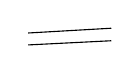
\begin{tikzpicture}[x=1em,y=1ex]\draw (0,0)--(3,.35);\draw (0,1)--(3,1.4);\end{tikzpicture}}}
The conditions  (ii)  and (iii) are equivalent and imply (i).

That (ii) implies (iii) is trivial by taking $I = i^{*}(\hand{\ensuremath{\Delta}}_{1})$ ;  the conver-%
se\hand{,} as we saw\hand{,} is a corollary of the comparison lemma for homotopy inter-%
vals  (p.60),  applied to  $I\hand{\ensuremath{\to}}i^{*}(\hand{\ensuremath{\Delta}}_{1}\ )$  corresponding to (12),  which is

%% END SOURCE ps_134-3_086
\ifnum\EditionMode=1
\psapparatusstart
\psentry{ps_134-3_086-v0001}{1}{insertion}{\inserted{weak}}{\hand{weak}}{The handwritten insertion is incorporated at its indicated position; insertion brackets leave the running text.}
\psentry{ps_134-3_086-v0002}{2}{insertion}{\inserted{weak}}{\hand{weak}}{The handwritten insertion is incorporated at its indicated position; insertion brackets leave the running text.}
\psentry{ps_134-3_086-v0003}{3}{insertion}{\inserted{$i_{A}i^{*}$}}{\hand{$i_{A}i^{*}$}}{The handwritten insertion is incorporated at its indicated position; insertion brackets leave the running text.}
\psentry{ps_134-3_086-v0004}{4}{typewriter deletion}{\xout{moreover}}{}{The typewriter strikes out this material; it leaves the corrected running text.}
\psentry{ps_134-3_086-v0005}{5}{typewriter overwriting}{\over[typed]{A}{i}}{i}{The superposed typed reading replaces the underlying reading.}
\psentry{ps_134-3_086-v0006}{6}{insertion}{\inserted{plus a little more still on i.}}{\hand{plus a little more still on i.}}{The handwritten insertion is incorporated at its indicated position; insertion brackets leave the running text.}
\psentry{ps_134-3_086-v0007}{7}{deletion}{\deleted{Then}}{}{The author cancels this material by hand; it leaves the corrected running text.}
\psentry{ps_134-3_086-v0008}{8}{insertion}{\inserted{Consider}}{\hand{Consider}}{The handwritten insertion is incorporated at its indicated position; insertion brackets leave the running text.}
\psentry{ps_134-3_086-v0009}{9}{deletion}{\deleted{are equivalent}}{}{The author cancels this material by hand; it leaves the corrected running text.}
\psentry{ps_134-3_086-v0010}{10}{typewriter deletion}{\xout{not}}{}{The typewriter strikes out this material; it leaves the corrected running text.}
\psentry{ps_134-3_086-v0011}{11}{typed insertion}{\inserted[typed]{weak}}{weak}{The typed insertion is incorporated at its indicated position; insertion brackets leave the running text.}
\psentry{ps_134-3_086-v0012}{12}{typewriter overwriting}{\over[typed]{H}{h}}{h}{The superposed typed reading replaces the underlying reading.}
\psentry{ps_134-3_086-v0013}{13}{writing over}{\over{A}{A}}{\hand{A}}{The superposed handwritten reading replaces the underlying reading.}
\psentry{ps_134-3_086-v0014}{14}{typewriter overwriting}{\over[typed]{i}{i}}{i}{The superposed typed reading replaces the underlying reading.}
\psentry{ps_134-3_086-v0015}{15}{typewriter overwriting}{\over[typed]{)}{)}}{)}{The superposed typed reading replaces the underlying reading.}
\psentry{ps_134-3_086-v0016}{16}{insertion}{\inserted{Moreover, A is aspheric.}}{\hand{Moreover, A is aspheric.}}{The handwritten insertion is incorporated at its indicated position; insertion brackets leave the running text.}
\psapparatusend
\fi
\pssource{ps_134-3_087}{134-3/87}{https://grothendieck.umontpellier.fr/web/viewer.html?file=../134-3.pdf\#page=88}
\psnumber{ps_134-3_087-v0001}{1}
\psnumber{ps_134-3_087-v0002}{2}
\psnumber{ps_134-3_087-v0003}{3}
\psnumber{ps_134-3_087-v0004}{4}
\psnumber{ps_134-3_087-v0005}{5}
\psnumber{ps_134-3_087-v0006}{6}
\psnumber{ps_134-3_087-v0007}{7}
\psnumber{ps_134-3_087-v0008}{8}
\psnumber{ps_134-3_087-v0009}{9}
\psnumber{ps_134-3_087-v0010}{10}
\psnumber{ps_134-3_087-v0011}{11}
\psnumber{ps_134-3_087-v0012}{12}
\psnumber{ps_134-3_087-v0013}{13}
\psnumber{ps_134-3_087-v0014}{14}
\psnumber{ps_134-3_087-v0015}{15}
%% BEGIN SOURCE ps_134-3_087
% Pursuing Stacks (cotes 134-2 to 134-8): archive cote 134-3, site page 87 (PDF page 88), typescript page 87.
% typescript. Draft compared: ps2.tex:4548-4619.
% AI-transcribed by Claude Opus 5.5 (claude-opus-5-5, adaptive thinking, effort high), Message Batches API, batch ps1 (msgbatch_01Rv5hCaNTtUt4JHx1yqoHPL), 2026-11-12; image review recorded in records/CHECK_DECISIONS_134_3_4.tsv.
\scanpage{134-3/87}
\mspage{\hand{87}}

a morphism of intervals\hand{,} namely compatible with endpoints. (However in prac\unsure{-}%
% NOTE: right edge of the scan cuts the end of this line after "prac"
tical terms (12) is the more ready-to-use criterion,  because in most
cases I will be in A and therefore  $i_{\hand{!}}(I) = i(I)$,  and (12) will be more
or less trivial,  for instance because I will be chosen so that $i(I)$ is
either $\hand{\Delta}_1 = \hand{\{0\}\to\{1\}}$  or it's barycentric subdivision \diagram{\begin{tikzcd}[row sep=-10pt,column sep=small] \{0\} \ar[dr] \& \\ \& \{0,1\} \\ \{1\} \ar[ur] \& \end{tikzcd}}.)  The
same argument shows that (iii) implies that A is a test category\hand{,} namely
the Lawvere element $L_A$ in $A^{\hand{\wedge}}$ is a homotopy interval in $A^{\hand{\wedge}}$\hand{,} namely is asphe-%
ric over $e_{A^{\hand{\wedge}}}$ .  This being so,  we \var{\xout{deduce that $i_A$ induces an}}{}{typewriter deletion}{ps_134-3_087-v0001} only got to
prove (under the assumption (iii))  that \var{\inserted{$i_Ai^*$}}{\hand{$i_Ai^*$}}{insertion}{ps_134-3_087-v0002} (11) induces an autoequivalence
of (Hot),  and more specifically a functor isomorphic to \var{the identify
functor}{the identity
functor}{slip corrected}{ps_134-3_087-v0003}\hand{.} \var{\inserted{This we achieved}}{\hand{This we achieved}}{insertion}{ps_134-3_087-v0004} by comparing directly $A_{\hand{/}C}$ to C  by the functor  $(a,p)\hand{\mapsto} p(e_a)$
(13) \qquad $A_{\hand{/}C} \hand{\longrightarrow} C$ ,
where  $e_a$ is the final element in $i(a)$.  It is enough to check this is a
weak equivalence for any C,  a fortiori that it is aspheric,  and the usu\var{\xout{\unsure{a}}}{}{typewriter deletion}{ps_134-3_087-v0005}%
al asphericity criterion reduces us to showing it is a weak equivalence
when C has a final object,  namely that in this case  $A_{\hand{/}C} = A_{\hand{/}i^{\hand{*}}(C)}$  is
aspheric,  i.e. $i^*(\unsure{\var{\over[typed]{A}{C}}{C}{typewriter overwriting}{ps_134-3_087-v0006}})$ is aspheric in $A^{\hand{\wedge}}$.  This was achieved by an extreme-%
ly simple homotopy argument,  using a homotopy  in (Cat)
\[ \hand{\Delta}_1 \mathrm{x} C \hand{\to} C \]
between the identity functor in C and the constant functor with value $e_C$ ;
(cf p. 62).

I feel like reserving the appe\hand{\unsure{ll}}ation of a \uline{test functor}  A $\hand{\longrightarrow}$ (Cat)
(in contrast to a \uline{weak} test functor)  to functors satisfying the equiva-%
lent conditions (ii) and (iii),  implying that A is a test category (not
merely a weak one ! ),  and which seem stronger a priori than assuming
\var{\deleted{moreover}}{}{deletion}{ps_134-3_087-v0007} \var{\inserted{(besides A being a \deleted{weak} test category)}}{\hand{(besides A being a  test category)}}{insertion}{ps_134-3_087-v0008} that i is a weak test functor  (condition (i)).  I confess I did
not make up my mind if \var{\xout{this}}{}{typewriter deletion}{ps_134-3_087-v0009} for a test category A , there may be weak
test functors,  with all i(a) having final objects,  which are not test
functors in the present sense,  namely whether it may be true that \var{\xout{all}}{}{typewriter deletion}{ps_134-3_087-v0010} for
\var{\xout{categories}}{}{typewriter deletion}{ps_134-3_087-v0011} \var{\inserted[typed]{any C in (Cat)}}{any C in (Cat)}{typed insertion}{ps_134-3_087-v0012}  with final object,  $i^*(C)$ is aspheric,  and \var{\xout{however}}{}{typewriter deletion}{ps_134-3_087-v0013} there-%
fore $i^*(\hand{\Delta}_1)$ aspheric,  without the \var{\over{m}{l}}{\hand{l}}{writing over}{ps_134-3_087-v0014}atter being aspheric over $e_{A^{\hand{\wedge}}}$ i.e.
all products $i^*(\hand{\Delta}_1) \mathrm{x} a$  ($a \hand{\in}$ Ob A) being aspheric \var{\inserted{(which would be automatic though \inserted{if A is even a \uline{strict} test category})}}{\hand{(which would be automatic though \hand{if A is even a \uline{strict} test category})}}{insertion}{ps_134-3_087-v0015}.  The difficulty here
is that it looks hard to check the condition for arbitrary C with final
object,  except through the homotopy argument using relative asphericity
of $i^*(\hand{\Delta}_1)$ .  Of course the distinction between weak test functors and test
functors is meaningful only as long as it is expected that the two are
actually distinct,  when applied to test categories.  Besides this,  the
restriction to categories i(a) with final objects looks theoretically a
little awkward,  and it should'nt be too hard I believe to get rid of it,
if need be.  But for the time being the only would-be test functors or

%% END SOURCE ps_134-3_087
\ifnum\EditionMode=1
\psapparatusstart
\psentry{ps_134-3_087-v0001}{1}{typewriter deletion}{\xout{deduce that $i_A$ induces an}}{}{The typewriter strikes out this material; it leaves the corrected running text.}
\psentry{ps_134-3_087-v0002}{2}{insertion}{\inserted{$i_Ai^*$}}{\hand{$i_Ai^*$}}{The handwritten insertion is incorporated at its indicated position; insertion brackets leave the running text.}
\psentry{ps_134-3_087-v0003}{3}{slip corrected}{the identify
functor}{the identity
functor}{The wrong f for t is settled by the same phrase identity functor later on this page.}
\psentry{ps_134-3_087-v0004}{4}{insertion}{\inserted{This we achieved}}{\hand{This we achieved}}{The handwritten insertion is incorporated at its indicated position; insertion brackets leave the running text.}
\psentry{ps_134-3_087-v0005}{5}{typewriter deletion}{\xout{\unsure{a}}}{}{The typewriter strikes out this material; it leaves the corrected running text.}
\psentry{ps_134-3_087-v0006}{6}{typewriter overwriting}{$\over[typed]{A}{C}$}{$C$}{The superposed typed reading replaces the underlying reading.}
\psentry{ps_134-3_087-v0007}{7}{deletion}{\deleted{moreover}}{}{The author cancels this material by hand; it leaves the corrected running text.}
\psentry{ps_134-3_087-v0008}{8}{insertion}{\inserted{(besides A being a \deleted{weak} test category)}}{\hand{(besides A being a  test category)}}{The handwritten insertion is incorporated at its indicated position; insertion brackets leave the running text.}
\psentry{ps_134-3_087-v0009}{9}{typewriter deletion}{\xout{this}}{}{The typewriter strikes out this material; it leaves the corrected running text.}
\psentry{ps_134-3_087-v0010}{10}{typewriter deletion}{\xout{all}}{}{The typewriter strikes out this material; it leaves the corrected running text.}
\psentry{ps_134-3_087-v0011}{11}{typewriter deletion}{\xout{categories}}{}{The typewriter strikes out this material; it leaves the corrected running text.}
\psentry{ps_134-3_087-v0012}{12}{typed insertion}{\inserted[typed]{any C in (Cat)}}{any C in (Cat)}{The typed insertion is incorporated at its indicated position; insertion brackets leave the running text.}
\psentry{ps_134-3_087-v0013}{13}{typewriter deletion}{\xout{however}}{}{The typewriter strikes out this material; it leaves the corrected running text.}
\psentry{ps_134-3_087-v0014}{14}{writing over}{\over{m}{l}}{\hand{l}}{The superposed handwritten reading replaces the underlying reading.}
\psentry{ps_134-3_087-v0015}{15}{insertion}{\inserted{(which would be automatic though \inserted{if A is even a \uline{strict} test category})}}{\hand{(which would be automatic though \hand{if A is even a \uline{strict} test category})}}{The handwritten insertion is incorporated at its indicated position; insertion brackets leave the running text.}
\psapparatusend
\fi
\pssource{ps_134-3_088}{134-3/88}{https://grothendieck.umontpellier.fr/web/viewer.html?file=../134-3.pdf\#page=89}
\psnumber{ps_134-3_088-v0001}{1}
\psnumber{ps_134-3_088-v0002}{2}
\psnumber{ps_134-3_088-v0003}{3}
\psnumber{ps_134-3_088-v0004}{4}
\psnumber{ps_134-3_088-v0005}{5}
\psnumber{ps_134-3_088-v0006}{6}
\psnumber{ps_134-3_088-v0007}{7}
\psnumber{ps_134-3_088-v0008}{8}
\psnumber{ps_134-3_088-v0009}{9}
\psnumber{ps_134-3_088-v0010}{10}
\psnumber{ps_134-3_088-v0011}{11}
\psnumber{ps_134-3_088-v0012}{12}
\psnumber{ps_134-3_088-v0013}{13}
\psnumber{ps_134-3_088-v0014}{14}
\psnumber{ps_134-3_088-v0015}{15}
\psnumber{ps_134-3_088-v0016}{16}
\psnumber{ps_134-3_088-v0017}{17}
\psnumber{ps_134-3_088-v0018}{18}
\psnumber{ps_134-3_088-v0019}{19}
\psnumber{ps_134-3_088-v0020}{20}
\psnumber{ps_134-3_088-v0021}{21}
\psnumber{ps_134-3_088-v0022}{22}
\psnumber{ps_134-3_088-v0023}{23}
\psnumber{ps_134-3_088-v0024}{24}
\psnumber{ps_134-3_088-v0025}{25}
\psnumber{ps_134-3_088-v0026}{26}
\psnumber{ps_134-3_088-v0027}{27}
\psnumber{ps_134-3_088-v0028}{28}
\psnumber{ps_134-3_088-v0029}{29}
\psnumber{ps_134-3_088-v0030}{30}
\psnumber{ps_134-3_088-v0031}{31}
\psnumber{ps_134-3_088-v0032}{32}
\psnumber{ps_134-3_088-v0033}{33}
\psnumber{ps_134-3_088-v0034}{34}
\psnumber{ps_134-3_088-v0035}{35}
\psnumber{ps_134-3_088-v0036}{36}
\psnumber{ps_134-3_088-v0037}{37}
\psnumber{ps_134-3_088-v0038}{38}
\psnumber{ps_134-3_088-v0039}{39}
\psnumber{ps_134-3_088-v0040}{40}
\psnumber{ps_134-3_088-v0041}{41}
\psnumber{ps_134-3_088-v0042}{42}
\psnumber{ps_134-3_088-v0043}{43}
\psnumber{ps_134-3_088-v0044}{44}
%% BEGIN SOURCE ps_134-3_088
% Pursuing Stacks (cotes 134-2 to 134-8): archive cote 134-3, site page 88 (PDF page 89), typescript page 88.
% typescript. Draft compared: ps2.tex:4603-4664.
% AI-transcribed by Claude Opus 5.5 (claude-opus-5-5, adaptive thinking, effort high), Message Batches API, batch ps1 (msgbatch_01Rv5hCaNTtUt4JHx1yqoHPL), 2026-11-12; image review recorded in records/CHECK_DECISIONS_134_3_4.tsv.
\scanpage{134-3/88}
\mspage{88}
weak test functors which have turned up,  do satisfy this condition,  \var{\xout{\unsure{then}}}{}{typewriter deletion}{ps_134-3_088-v0001}
therefore it \unsure{does'nt|does(nt} seem urgent to clean up the notion in this respect.
\var{\inserted{\uline{Remarks.}}}{\hand{\uline{Remarks.}}}{insertion}{ps_134-3_088-v0002}
\hand{1.} I regret I was slightly floppy when translating the condition  that
\var{\xout{(xxx)}}{}{typewriter deletion}{ps_134-3_088-v0003}\var{\inserted{$\phi =$}}{\hand{$\phi =$}}{insertion}{ps_134-3_088-v0004} $i_A i^*$  (11)  be model-preserving,  by the (a priori less precise)
co\var{\over[typed]{j}{n}}{n}{typewriter overwriting}{ps_134-3_088-v0005}d\unsure{it}ion that it induce an autoequivalence of the localized category
(Hot)\unsure{\var{\over{,}{;}}{\hand{;}}{writing over}{ps_134-3_088-v0006}}\hand{(}which is of course meant to imply that it transforms weak equiva-%
lences into weak equivalences,  and thus does induce a functor from (Hot)
into itself\hand{)}. \var{\deleted{But}}{}{deletion}{ps_134-3_088-v0007} \var{\over{i}{I}}{\hand{I}}{writing over}{ps_134-3_088-v0008}t is'nt clear that if this functor is an equivalence,
then  $W = \phi^{-1}(W)$,  except if we admit that W is strongly saturated  i.e.
an arrow in (Cat) which becomes an isomorphism in (Hot),  is indeed a
quasi-equivalence.  This,\var{\xout{as}}{}{typewriter deletion}{ps_134-3_088-v0009} as we saw,  follows from the fact that there
are \var{\inserted[typed]{weak}}{weak}{typed insertion}{ps_134-3_088-v0010} test categories (such as \hand{\ensuremath{\Delta}} , which is even a strict one)\hand{,} such that
A\hand{\ensuremath{^{\wedge}}}  be a ``closed model category'' in Quillen's sense  -  but I did'nt check
yet in the present set-up that \hand{\ensuremath{\Delta}}\hand{\ensuremath{^{\wedge}}} does indeed satisfy Quillen's condition.
\uline{Which} elementary modelizers are ``closed model categories'' remains one of
the intriguing questions in this homotopy model story,  which I'll have to
look into pretty soon now.

\var{\deleted{\hand{Remarks}}}{}{deletion}{ps_134-3_088-v0011}
\hand{2.} It should be noted that \var{\xout{if}}{}{typewriter deletion}{ps_134-3_088-v0012}\var{\deleted{\hand{even}}}{}{deletion}{ps_134-3_088-v0013} if i: A\hand{\ensuremath{\to}}(Cat) is a test functor, \hand{even}
with a strict test category \hand{A}\hand{(}such as \hand{\ensuremath{\Delta}} ,  with the standart embedding
i of \hand{\ensuremath{\Delta}}  into (Cat) \var{\inserted{say}}{\hand{say}}{insertion}{ps_134-3_088-v0014}\hand{)},  whereas  $i^*$ : (Cat)\hand{\ensuremath{\to}} A\hand{\ensuremath{^{\wedge}}} is model preserving by \var{\xout{the}}{}{typewriter deletion}{ps_134-3_088-v0015}
definition,  it is by no means always true that the \var{\inserted[typed]{left}}{left}{typed insertion}{ps_134-3_088-v0016} adjoint functor
\[ i_{\hand{!}} \ : \ A^{\hand{\wedge}}\hand{\ensuremath{\to}} (Cat) \]
(which can be equally defined as the canonical extension of i to A\hand{\ensuremath{^{\wedge}}},  commu-%
ting with direct limits)  is equally model preserving.  This seems to be
in fact an extremely special property of \var{\inserted{just}}{\hand{just}}{insertion}{ps_134-3_088-v0017} the ``canonical'' test functor $i_A$\hand{\ensuremath{|A}}.
\hand{3.} On the other hand,  I do not know if for any small category \var{\inserted{A,}}{\hand{A,}}{insertion}{ps_134-3_088-v0018} such that
(A\hand{\ensuremath{^{\wedge}}}\var{\xout{\unsure{x}}}{}{typewriter deletion}{ps_134-3_088-v0019} , $W_A = W_{A^{\hand{\wedge}}}$)  is a modelizer and $i_A$: A\hand{\ensuremath{^{\wedge}}} \hand{\ensuremath{\to}}(Cat)  is model preserving, A
\var{\xout{(or $j_A$ (Cat) A\hand{\ensuremath{^{\wedge}}} is model preserving) if}}{}{typewriter deletion}{ps_134-3_088-v0020} is a weak test category\var{\over{,}{.}}{\hand{.}}{writing over}{ps_134-3_088-v0021}
\var{\deleted{\xout{Also, even assuming that A is a weak test category. However, if we}}}{}{deletion}{ps_134-3_088-v0022} \var{\inserted{However, if we}}{\hand{However, if we}}{insertion}{ps_134-3_088-v0023}
\var{\deleted{and moreover A aspheric}}{}{deletion}{ps_134-3_088-v0024} \var{\deleted{\hand{and A aspheric}}}{}{deletion}{ps_134-3_088-v0025}
assume that $j_A$\var{\inserted{$=i_A^*$}}{\hand{$=i_A^*$}}{insertion}{ps_134-3_088-v0026}: (Cat)\hand{\ensuremath{\to}} A\hand{\ensuremath{^{\wedge}}} is model preserving \var{\inserted{(and moreover A aspheric)}}{\hand{(and moreover A aspheric)}}{insertion}{ps_134-3_088-v0027},  then A is a weak test
category,  because $j_A$  transforms weak equivalences into weak equivalences
\var{\deleted{\hand{and final object of (Hot) into a final object,}}}{}{deletion}{ps_134-3_088-v0028}
\hand{(}and we apply criterion (vii) (p. 80).) \var{\xout{We still have to check that A is}}{}{typewriter deletion}{ps_134-3_088-v0029}
\var{\xout{aspheric i.e. that the induced functor}}{}{typewriter deletion}{ps_134-3_088-v0030} M$\overset{\hand{\smile}}{\mathrm{o}}$re generally ,  if we have a
functor  i:  A\var{\deleted{\hand{\ensuremath{^{\wedge}}}}}{}{deletion}{ps_134-3_088-v0031}\hand{\ensuremath{\to}}(Cat)  such that $i^*$ : (Cat)\hand{\ensuremath{\to}} A\hand{\ensuremath{^{\wedge}}} is model preserving
(assuming already (A\hand{\ensuremath{^{\wedge}}};$W_A$) to be a \hand{``}modelizer\hand{''}),  \var{\inserted{I wonder}}{\hand{I wonder}}{insertion}{ps_134-3_088-v0032} whether this implies that
A is already a weak test category\hand{,}\var{\deleted{\hand{?}}}{}{deletion}{ps_134-3_088-v0033}  as it does when i is the canonical
functor $i_A$ and hence $i^* = j_A$ \hand{.} \var{\deleted{(at least if we assume A to be aspheric,}}{}{deletion}{ps_134-3_088-v0034} \var{\inserted{The answer is'nt clear to me even when}}{\hand{The answer is'nt clear to me even when}}{insertion}{ps_134-3_088-v0035}
\var{\inserted{assuming}}{\hand{assuming}}{insertion}{ps_134-3_088-v0036} \var{\deleted{which I am quite willing to add anyhow,}}{}{deletion}{ps_134-3_088-v0037} \var{\deleted{\hand{and even that}}}{}{deletion}{ps_134-3_088-v0038} \var{\deleted{\illegible{1}}}{}{deletion}{ps_134-3_088-v0039} \hand{$i_A$, or equivalently}
\hand{$\varphi = i_A i^*$, is model-preserving too.} \var{\deleted{\hand{\illegible{1}}}}{}{deletion}{ps_134-3_088-v0040}
\var{\deleted{\hand{4.}}}{}{deletion}{ps_134-3_088-v0041} \var{\deleted{It occured to me \deleted{too} that  condition (i) on p.79,  and even the wea-}}{}{deletion}{ps_134-3_088-v0042}%
\var{\deleted{ker form (i') (p.81)  does indeed imply the others, namely asphericity of}}{}{deletion}{ps_134-3_088-v0043}
\var{\deleted{A,  because an autoequivalence of (Hot) respects final objects !}}{}{deletion}{ps_134-3_088-v0044}

%% END SOURCE ps_134-3_088
\ifnum\EditionMode=1
\psapparatusstart
\psentry{ps_134-3_088-v0001}{1}{typewriter deletion}{\xout{\unsure{then}}}{}{The typewriter strikes out this material; it leaves the corrected running text.}
\psentry{ps_134-3_088-v0002}{2}{insertion}{\inserted{\uline{Remarks.}}}{\hand{\uline{Remarks.}}}{The handwritten insertion is incorporated at its indicated position; insertion brackets leave the running text.}
\psentry{ps_134-3_088-v0003}{3}{typewriter deletion}{\xout{(xxx)}}{}{The typewriter strikes out this material; it leaves the corrected running text.}
\psentry{ps_134-3_088-v0004}{4}{insertion}{\inserted{$\phi =$}}{\hand{$\phi =$}}{The handwritten insertion is incorporated at its indicated position; insertion brackets leave the running text.}
\psentry{ps_134-3_088-v0005}{5}{typewriter overwriting}{\over[typed]{j}{n}}{n}{The superposed typed reading replaces the underlying reading.}
\psentry{ps_134-3_088-v0006}{6}{writing over}{\over{,}{;}}{\hand{;}}{The superposed handwritten reading replaces the underlying reading.}
\psentry{ps_134-3_088-v0007}{7}{deletion}{\deleted{But}}{}{The author cancels this material by hand; it leaves the corrected running text.}
\psentry{ps_134-3_088-v0008}{8}{writing over}{\over{i}{I}}{\hand{I}}{The superposed handwritten reading replaces the underlying reading.}
\psentry{ps_134-3_088-v0009}{9}{typewriter deletion}{\xout{as}}{}{The typewriter strikes out this material; it leaves the corrected running text.}
\psentry{ps_134-3_088-v0010}{10}{typed insertion}{\inserted[typed]{weak}}{weak}{The typed insertion is incorporated at its indicated position; insertion brackets leave the running text.}
\psentry{ps_134-3_088-v0011}{11}{deletion}{\deleted{\hand{Remarks}}}{}{The author cancels this material by hand; it leaves the corrected running text.}
\psentry{ps_134-3_088-v0012}{12}{typewriter deletion}{\xout{if}}{}{The typewriter strikes out this material; it leaves the corrected running text.}
\psentry{ps_134-3_088-v0013}{13}{deletion}{\deleted{\hand{even}}}{}{The author cancels this material by hand; it leaves the corrected running text.}
\psentry{ps_134-3_088-v0014}{14}{insertion}{\inserted{say}}{\hand{say}}{The handwritten insertion is incorporated at its indicated position; insertion brackets leave the running text.}
\psentry{ps_134-3_088-v0015}{15}{typewriter deletion}{\xout{the}}{}{The typewriter strikes out this material; it leaves the corrected running text.}
\psentry{ps_134-3_088-v0016}{16}{typed insertion}{\inserted[typed]{left}}{left}{The typed insertion is incorporated at its indicated position; insertion brackets leave the running text.}
\psentry{ps_134-3_088-v0017}{17}{insertion}{\inserted{just}}{\hand{just}}{The handwritten insertion is incorporated at its indicated position; insertion brackets leave the running text.}
\psentry{ps_134-3_088-v0018}{18}{insertion}{\inserted{A,}}{\hand{A,}}{The handwritten insertion is incorporated at its indicated position; insertion brackets leave the running text.}
\psentry{ps_134-3_088-v0019}{19}{typewriter deletion}{\xout{\unsure{x}}}{}{The typewriter strikes out this material; it leaves the corrected running text.}
\psentry{ps_134-3_088-v0020}{20}{typewriter deletion}{\xout{(or $j_A$ (Cat) A\hand{\ensuremath{^{\wedge}}} is model preserving) if}}{}{The typewriter strikes out this material; it leaves the corrected running text.}
\psentry{ps_134-3_088-v0021}{21}{writing over}{\over{,}{.}}{\hand{.}}{The superposed handwritten reading replaces the underlying reading.}
\psentry{ps_134-3_088-v0022}{22}{deletion}{\deleted{\xout{Also, even assuming that A is a weak test category. However, if we}}}{}{The author cancels this material by hand; it leaves the corrected running text.}
\psentry{ps_134-3_088-v0023}{23}{insertion}{\inserted{However, if we}}{\hand{However, if we}}{The handwritten insertion is incorporated at its indicated position; insertion brackets leave the running text.}
\psentry{ps_134-3_088-v0024}{24}{deletion}{\deleted{and moreover A aspheric}}{}{The author cancels this material by hand; it leaves the corrected running text.}
\psentry{ps_134-3_088-v0025}{25}{deletion}{\deleted{\hand{and A aspheric}}}{}{The author cancels this material by hand; it leaves the corrected running text.}
\psentry{ps_134-3_088-v0026}{26}{insertion}{\inserted{$=i_A^*$}}{\hand{$=i_A^*$}}{The handwritten insertion is incorporated at its indicated position; insertion brackets leave the running text.}
\psentry{ps_134-3_088-v0027}{27}{insertion}{\inserted{(and moreover A aspheric)}}{\hand{(and moreover A aspheric)}}{The handwritten insertion is incorporated at its indicated position; insertion brackets leave the running text.}
\psentry{ps_134-3_088-v0028}{28}{deletion}{\deleted{\hand{and final object of (Hot) into a final object,}}}{}{The author cancels this material by hand; it leaves the corrected running text.}
\psentry{ps_134-3_088-v0029}{29}{typewriter deletion}{\xout{We still have to check that A is}}{}{The typewriter strikes out this material; it leaves the corrected running text.}
\psentry{ps_134-3_088-v0030}{30}{typewriter deletion}{\xout{aspheric i.e. that the induced functor}}{}{The typewriter strikes out this material; it leaves the corrected running text.}
\psentry{ps_134-3_088-v0031}{31}{deletion}{\deleted{\hand{\ensuremath{^{\wedge}}}}}{}{The author cancels this material by hand; it leaves the corrected running text.}
\psentry{ps_134-3_088-v0032}{32}{insertion}{\inserted{I wonder}}{\hand{I wonder}}{The handwritten insertion is incorporated at its indicated position; insertion brackets leave the running text.}
\psentry{ps_134-3_088-v0033}{33}{deletion}{\deleted{\hand{?}}}{}{The author cancels this material by hand; it leaves the corrected running text.}
\psentry{ps_134-3_088-v0034}{34}{deletion}{\deleted{(at least if we assume A to be aspheric,}}{}{The author cancels this material by hand; it leaves the corrected running text.}
\psentry{ps_134-3_088-v0035}{35}{insertion}{\inserted{The answer is'nt clear to me even when}}{\hand{The answer is'nt clear to me even when}}{The handwritten insertion is incorporated at its indicated position; insertion brackets leave the running text.}
\psentry{ps_134-3_088-v0036}{36}{insertion}{\inserted{assuming}}{\hand{assuming}}{The handwritten insertion is incorporated at its indicated position; insertion brackets leave the running text.}
\psentry{ps_134-3_088-v0037}{37}{deletion}{\deleted{which I am quite willing to add anyhow,}}{}{The author cancels this material by hand; it leaves the corrected running text.}
\psentry{ps_134-3_088-v0038}{38}{deletion}{\deleted{\hand{and even that}}}{}{The author cancels this material by hand; it leaves the corrected running text.}
\psentry{ps_134-3_088-v0039}{39}{deletion}{\deleted{\illegible{1}}}{}{The author cancels this material by hand; it leaves the corrected running text.}
\psentry{ps_134-3_088-v0040}{40}{deletion}{\deleted{\hand{\illegible{1}}}}{}{The author cancels this material by hand; it leaves the corrected running text.}
\psentry{ps_134-3_088-v0041}{41}{deletion}{\deleted{\hand{4.}}}{}{The author cancels this material by hand; it leaves the corrected running text.}
\psentry{ps_134-3_088-v0042}{42}{deletion}{\deleted{It occured to me \deleted{too} that  condition (i) on p.79,  and even the wea-}}{}{The author cancels this material by hand; it leaves the corrected running text.}
\psentry{ps_134-3_088-v0043}{43}{deletion}{\deleted{ker form (i') (p.81)  does indeed imply the others, namely asphericity of}}{}{The author cancels this material by hand; it leaves the corrected running text.}
\psentry{ps_134-3_088-v0044}{44}{deletion}{\deleted{A,  because an autoequivalence of (Hot) respects final objects !}}{}{The author cancels this material by hand; it leaves the corrected running text.}
\psapparatusend
\fi
\pssource{ps_134-3_089}{134-3/89}{https://grothendieck.umontpellier.fr/web/viewer.html?file=../134-3.pdf\#page=90}
\psnumber{ps_134-3_089-v0001}{1}
\psnumber{ps_134-3_089-v0002}{2}
\psnumber{ps_134-3_089-v0003}{3}
\psnumber{ps_134-3_089-v0004}{4}
\psnumber{ps_134-3_089-v0005}{5}
\psnumber{ps_134-3_089-v0006}{6}
\psnumber{ps_134-3_089-v0007}{7}
\psnumber{ps_134-3_089-v0008}{8}
\psnumber{ps_134-3_089-v0009}{9}
\psnumber{ps_134-3_089-v0010}{10}
\psnumber{ps_134-3_089-v0011}{11}
\psnumber{ps_134-3_089-v0012}{12}
\psnumber{ps_134-3_089-v0013}{13}
%% BEGIN SOURCE ps_134-3_089
% Pursuing Stacks (cotes 134-2 to 134-8): archive cote 134-3, site page 89 (PDF page 90).
% notes for ch. II. Draft compared: ps2.tex:98-116 ; ps2.tex:125-138 ; ps2.tex:144-175.
% AI-transcribed by Claude Opus 5.5 (claude-opus-5-5, adaptive thinking, effort high), Message Batches API, batch ps1 (msgbatch_01Rv5hCaNTtUt4JHx1yqoHPL), 2026-11-12; image review recorded in records/CHECK_DECISIONS_134_3_4.tsv.
\scanpage{134-3/89}
\mspage{\hand{I}I (i)}

\uline{Notes for Chapter} I\hand{I}

(\textsuperscript{1}) For another way of viewing the role of the Hauptvermutung, namely
``rehab\var{\over[typed]{\unsure{o}}{i}}{i}{typewriter overwriting}{ps_134-3_089-v0001}litating'' it as being essentially valid, see note (\textsuperscript{6}) at the end
of Esquisse d'un Programme (in RM 1 ).

(\textsuperscript{2}) As a matter of fact, it is pretty obvious today how to get the
Leray spectral sequence directly in the semisimplicial set-up\hand{,}without
using cubes,

(\textsuperscript{3}) Ronnie Brown pointed out to me that ``Dold-Puppe'' is an inaccurate
\var{\xout{desi}}{}{typewriter deletion}{ps_134-3_089-v0002} name here, as this theorem has been found \var{\over{u}{i}}{\hand{i}}{writing over}{ps_134-3_089-v0003}ndependently by Dold and
Kan. I have corrected this unaccuracy in later occurences in my type-%
script, writing ``Dold-Kan'' instead.

(\textsuperscript{4}) \var{\deleted{(Added 3.5.1984.)}}{}{deletion}{ps_134-3_089-v0004} This statement is mistaken - it appeared soon
after that the cohomology of a stack can be expressed in terms of the
``prim\var{\over[typed]{a}{i}}{i}{typewriter overwriting}{ps_134-3_089-v0005}\var{\over{t}{t}}{\hand{t}}{writing over}{ps_134-3_089-v0006}\var{\over{\unsure{j}}{i}}{\hand{i}}{writing over}{ps_134-3_089-v0007}\var{\inserted[typed]{ve}}{ve}{typed insertion}{ps_134-3_089-v0008} structure'' (just face operations) much in the same way as for
simplicial or cubical complexes - it is even simpler, because in each
dimension there are only two face operators (whose formal difference will
be the boundary operator). It is at this point that the idea of ``\uline{hemis-}%
\uline{pherical complexes}'' (or \hand{``}h.''sets'') comes in very naturally, as the kind
of objects that remain, when a ``stack'' is stripped from all it's structu-%
re except the primitive structure, namely a family of objects $(F_i)$ toge-%
ther with the ``face operations'' $(s_i,t_i)$ $(i \hand{\ensuremath{\geq}} 1)$, namely the ``source'' and
``target'' maps - plus, preferably, also the degeneracies $k_i$ $(i \hand{\ensuremath{\geq}} 0)$, one
in each dimension. These may be viewed too as the objects in \hand{\ensuremath{\mathord{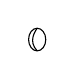
\begin{tikzpicture}[x=1ex,y=1ex,baseline=-.5ex]\draw (0,0) ellipse (.72 and .95);\draw (0,-.95) .. controls (-.75,-.15) and (-.2,.65) .. (0,.95);\end{tikzpicture}}}}\hand{\ensuremath{^{\wedge}}}, where
\hand{\ensuremath{\mathord{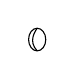
\begin{tikzpicture}[x=1ex,y=1ex,baseline=-.5ex]\draw (0,0) ellipse (.72 and .95);\draw (0,-.95) .. controls (-.75,-.15) and (-.2,.65) .. (0,.95);\end{tikzpicture}}}} is the category of ``\uline{standard he\var{\over{mi}{mi}}{\hand{mi}}{writing over}{ps_134-3_089-v0009}spheres}'', very similar to the catego-%
ries \hand{\ensuremath{\Delta}} and \hand{\ensuremath{\square}} of standard simplices resp. cubes, and even simpler than
these (being based on bigons, rather than \var{\inserted{on}}{\hand{on}}{insertion}{ps_134-3_089-v0010} triangles or squares). In the
sequel, we often refer to this category \hand{\ensuremath{\mathord{\begin{tikzpicture}[x=1ex,y=1ex,baseline=-.5ex]\draw (0,0) ellipse (.72 and .95);\draw (0,-.95) .. controls (-.75,-.15) and (-.2,.65) .. (0,.95);\end{tikzpicture}}}}, and to the ``trinity'' of the
three most beautiful ``test categories'' (in fact, they are even ``contrac-%
tors'')\hand{\ensuremath{\mathord{\begin{tikzpicture}[x=1ex,y=1ex,baseline=-.5ex]\draw (0,0) ellipse (.72 and .95);\draw (0,-.95) .. controls (-.75,-.15) and (-.2,.65) .. (0,.95);\end{tikzpicture}}}} ,\hand{\ensuremath{\Delta}} ,\hand{\ensuremath{\square}}, without having introduced formally \hand{\ensuremath{\mathord{\begin{tikzpicture}[x=1ex,y=1ex,baseline=-.5ex]\draw (0,0) ellipse (.72 and .95);\draw (0,-.95) .. controls (-.75,-.15) and (-.2,.65) .. (0,.95);\end{tikzpicture}}}} anywhere in the
notes. \var{\xout{As a matt}}{}{typewriter deletion}{ps_134-3_089-v0011} This category \hand{\ensuremath{\mathord{\begin{tikzpicture}[x=1ex,y=1ex,baseline=-.5ex]\draw (0,0) ellipse (.72 and .95);\draw (0,-.95) .. controls (-.75,-.15) and (-.2,.65) .. (0,.95);\end{tikzpicture}}}} has been first introduced in the the-%
sis of \uline{David} W. \uline{Jones} (a student of Ronnie Brown) ``\uline{Poly T-Complexes}'' ,
\var{\xout{under the name of}}{}{typewriter deletion}{ps_134-3_089-v0012} and he calls the corresponding notion of complexes
``\uline{globular} complexes'' (instead of ``hemispherical''). That these do modeli-%
ze homotopy types, more accurately that \hand{\ensuremath{\mathord{\begin{tikzpicture}[x=1ex,y=1ex,baseline=-.5ex]\draw (0,0) ellipse (.72 and .95);\draw (0,-.95) .. controls (-.75,-.15) and (-.2,.65) .. (0,.95);\end{tikzpicture}}}} is a (stric\var{\over{\unsure{t}}{t}}{\hand{t}}{writing over}{ps_134-3_089-v0013}) test category,
will follow from the general criterion of section 31, much in the same
way as for\hand{\ensuremath{\Delta}} and \hand{\ensuremath{\square}}(see section 34 for these). It is clear that for the
study of stacks, hemispherical complexes will be better suited than
semisimplicial or cubical ones. It should'nt be hard anyhow to describe
functors going from one type of complexes to the other, in such a way \margin{\diagram{\begin{tikzpicture}[x=.8em,y=.7ex]\draw (.6,3)--(0,2.6) .. controls (-.3,1.4) and (.9,1.7) .. (.55,.8)--(0,.2)--(.2,-.5);\draw (.05,2.2)--(.65,2.4);\end{tikzpicture}}}

\mspage{\hand{89}}

%% END SOURCE ps_134-3_089
\ifnum\EditionMode=1
\psapparatusstart
\psentry{ps_134-3_089-v0001}{1}{typewriter overwriting}{\over[typed]{\unsure{o}}{i}}{i}{The superposed typed reading replaces the underlying reading.}
\psentry{ps_134-3_089-v0002}{2}{typewriter deletion}{\xout{desi}}{}{The typewriter strikes out this material; it leaves the corrected running text.}
\psentry{ps_134-3_089-v0003}{3}{writing over}{\over{u}{i}}{\hand{i}}{The superposed handwritten reading replaces the underlying reading.}
\psentry{ps_134-3_089-v0004}{4}{deletion}{\deleted{(Added 3.5.1984.)}}{}{The author cancels this material by hand; it leaves the corrected running text.}
\psentry{ps_134-3_089-v0005}{5}{typewriter overwriting}{\over[typed]{a}{i}}{i}{The superposed typed reading replaces the underlying reading.}
\psentry{ps_134-3_089-v0006}{6}{writing over}{\over{t}{t}}{\hand{t}}{The superposed handwritten reading replaces the underlying reading.}
\psentry{ps_134-3_089-v0007}{7}{writing over}{\over{\unsure{j}}{i}}{\hand{i}}{The superposed handwritten reading replaces the underlying reading.}
\psentry{ps_134-3_089-v0008}{8}{typed insertion}{\inserted[typed]{ve}}{ve}{The typed insertion is incorporated at its indicated position; insertion brackets leave the running text.}
\psentry{ps_134-3_089-v0009}{9}{writing over}{\over{mi}{mi}}{\hand{mi}}{The superposed handwritten reading replaces the underlying reading.}
\psentry{ps_134-3_089-v0010}{10}{insertion}{\inserted{on}}{\hand{on}}{The handwritten insertion is incorporated at its indicated position; insertion brackets leave the running text.}
\psentry{ps_134-3_089-v0011}{11}{typewriter deletion}{\xout{As a matt}}{}{The typewriter strikes out this material; it leaves the corrected running text.}
\psentry{ps_134-3_089-v0012}{12}{typewriter deletion}{\xout{under the name of}}{}{The typewriter strikes out this material; it leaves the corrected running text.}
\psentry{ps_134-3_089-v0013}{13}{writing over}{\over{\unsure{t}}{t}}{\hand{t}}{The superposed handwritten reading replaces the underlying reading.}
\psapparatusend
\fi
\pssource{ps_134-3_090}{134-3/90}{https://grothendieck.umontpellier.fr/web/viewer.html?file=../134-3.pdf\#page=91}
\psnumber{ps_134-3_090-v0001}{1}
\psnumber{ps_134-3_090-v0002}{2}
\psnumber{ps_134-3_090-v0003}{3}
\psnumber{ps_134-3_090-v0004}{4}
\psnumber{ps_134-3_090-v0005}{5}
\psnumber{ps_134-3_090-v0006}{6}
\psnumber{ps_134-3_090-v0007}{7}
\psnumber{ps_134-3_090-v0008}{8}
\psnumber{ps_134-3_090-v0009}{9}
\psnumber{ps_134-3_090-v0010}{10}
\psnumber{ps_134-3_090-v0011}{11}
\psnumber{ps_134-3_090-v0012}{12}
\psnumber{ps_134-3_090-v0013}{13}
\psnumber{ps_134-3_090-v0014}{14}
%% BEGIN SOURCE ps_134-3_090
% Pursuing Stacks (cotes 134-2 to 134-8): archive cote 134-3, site page 90 (PDF page 91).
% notes for ch. II. Draft compared: ps2.tex:175-184 ; ps2.tex:301-310 ; ps2.tex:328-349 ; ps2.tex:506-516.
% AI-transcribed by Claude Opus 5.5 (claude-opus-5-5, adaptive thinking, effort high), Message Batches API, batch ps1 (msgbatch_01Rv5hCaNTtUt4JHx1yqoHPL), 2026-11-12; image review recorded in records/CHECK_DECISIONS_134_3_4.tsv.
\scanpage{134-3/90}
II ii

that the homotopy types modelled by two complexes which correspond should
be canonically isomorphic. In terms of the theory of \hand{``}test-functors\hand{''} which
is to follow,  this amounts essentially to the question of finding an
explicit test functor \hand{\ensuremath{\Delta \to \widehat{\mathord{\begin{tikzpicture}[x=1ex,y=1ex,baseline=-.5ex]\draw (0,0) ellipse (.72 and .95);\draw (0,-.95) .. controls (-.75,-.15) and (-.2,.65) .. (0,.95);\end{tikzpicture}}}}} (and\hand{/}similarly in the five other cases).
This reminds me of the problem of giving handy existence and unicity
theorems for test functors,\var{\deleted{\unsure{f}}}{}{deletion}{ps_134-3_090-v0001} dwelled upon somewhat in section 90, but by
no means settled yet ...

($^5$)   Compare with my letter to Breen ( I App.7).

($^6$)   Compare with (I App.2).

($^7$)   The definition of the nerve functor,  realizing a full embedding
of (Cat) into \hand{\ensuremath{\Delta}}\hand{\ensuremath{^{\wedge}}}, is given for the first time \var{\inserted[typed]{(I believe)}}{(I believe)}{typed insertion}{ps_134-3_090-v0002} in a Bourbaki talk of mine
\margin{X} (\hspace{5em}),  which at that time was'nt concerned at all with the topo-%
logical interpretation of small categories,  but with \var{\xout{\unsure{that}}}{}{typewriter deletion}{ps_134-3_090-v0003} some rather
formal prerequisites for the operation of "passage to quotient" of an ob-%
je\var{\over[typed]{d}{c}}{c}{typewriter overwriting}{ps_134-3_090-v0004}t by a "pre-equivalence relation",  in any category (with a view of
applying it \var{\xout{to the}}{}{typewriter deletion}{ps_134-3_090-v0005} in the category of schemes ...).

(\hand{\unsure{!}}$^8$)   This is well known to be false,  and the mistake is corrected
later (section 24).  The next statement,  about (Cat) modelizing the homo-%
topy category,  is true however and has been fairly well known  (due to
Fri\var{\over[typed]{j}{t}}{t}{typewriter overwriting}{ps_134-3_090-v0006}sch and Latch, Ronnie Brown tells me).  In these notes,  it is going
to come out in section 34,  under the form "\hand{\ensuremath{\Delta}} is a test category",
using the general criterion for test categories obtained in section 31.

($^9$)   As seen a little later,  this \var{\inserted[typed]{tentative}}{tentative}{typed insertion}{ps_134-3_090-v0007} description of a suitable class of
cofibrations is unadequate (see  beginning of section 30).  An adequate
description of a closed model structure in (Cat) was found by \uline{Thomason}
(see comments on this in section 87).

($^{10}$)   Dispite th\var{\over[typed]{i}{i}}{i}{typewriter overwriting}{ps_134-3_090-v0008}s "feeling",  it turns out that the whole first volume
of "Pursuing Stacks" is spent on pursuing this general question o\var{\over{r}{f}}{\hand{f}}{writing over}{ps_134-3_090-v0009}
understanding homotopy models in general,  \var{\xout{rather than}}{}{typewriter deletion}{ps_134-3_090-v0010} while the stacks
are being forg\var{\over[typed]{t}{o}}{o}{typewriter overwriting}{ps_134-3_090-v0011}tten  for a thousand pages or so ...

($^{11}$)   Finally,  it turns out more suitable still to replace this cate-%
gory by the \var{\xout{still}}{}{typewriter deletion}{ps_134-3_090-v0012} smaller one of standard hemispheres \hand{\ensuremath{\mathord{\begin{tikzpicture}[x=1ex,y=1ex,baseline=-.5ex]\draw (0,0) ellipse (.72 and .95);\draw (0,-.95) .. controls (-.75,-.15) and (-.2,.65) .. (0,.95);\end{tikzpicture}}}},  compare ($^4$).

($^{12}$)   From a letter of Benabou which I got later,  I understand that he
got discouraged from pursuing his topological approach to n-categories,
because of the complete lack of interest of anybody else in this approach.
I was glad to hear from him last year that my present work has stimulated
him into starting a seminar on th\var{\over[typed]{e}{i}}{i}{typewriter overwriting}{ps_134-3_090-v0013}\var{\over[typed]{s}{s}}{s}{typewriter overwriting}{ps_134-3_090-v0014} topic of stacks,  using my notes as a
leading thread.

\mspage{\hand{90}}

%% END SOURCE ps_134-3_090
\ifnum\EditionMode=1
\psapparatusstart
\psentry{ps_134-3_090-v0001}{1}{deletion}{\deleted{\unsure{f}}}{}{The author cancels this material by hand; it leaves the corrected running text.}
\psentry{ps_134-3_090-v0002}{2}{typed insertion}{\inserted[typed]{(I believe)}}{(I believe)}{The typed insertion is incorporated at its indicated position; insertion brackets leave the running text.}
\psentry{ps_134-3_090-v0003}{3}{typewriter deletion}{\xout{\unsure{that}}}{}{The typewriter strikes out this material; it leaves the corrected running text.}
\psentry{ps_134-3_090-v0004}{4}{typewriter overwriting}{\over[typed]{d}{c}}{c}{The superposed typed reading replaces the underlying reading.}
\psentry{ps_134-3_090-v0005}{5}{typewriter deletion}{\xout{to the}}{}{The typewriter strikes out this material; it leaves the corrected running text.}
\psentry{ps_134-3_090-v0006}{6}{typewriter overwriting}{\over[typed]{j}{t}}{t}{The superposed typed reading replaces the underlying reading.}
\psentry{ps_134-3_090-v0007}{7}{typed insertion}{\inserted[typed]{tentative}}{tentative}{The typed insertion is incorporated at its indicated position; insertion brackets leave the running text.}
\psentry{ps_134-3_090-v0008}{8}{typewriter overwriting}{\over[typed]{i}{i}}{i}{The superposed typed reading replaces the underlying reading.}
\psentry{ps_134-3_090-v0009}{9}{writing over}{\over{r}{f}}{\hand{f}}{The superposed handwritten reading replaces the underlying reading.}
\psentry{ps_134-3_090-v0010}{10}{typewriter deletion}{\xout{rather than}}{}{The typewriter strikes out this material; it leaves the corrected running text.}
\psentry{ps_134-3_090-v0011}{11}{typewriter overwriting}{\over[typed]{t}{o}}{o}{The superposed typed reading replaces the underlying reading.}
\psentry{ps_134-3_090-v0012}{12}{typewriter deletion}{\xout{still}}{}{The typewriter strikes out this material; it leaves the corrected running text.}
\psentry{ps_134-3_090-v0013}{13}{typewriter overwriting}{\over[typed]{e}{i}}{i}{The superposed typed reading replaces the underlying reading.}
\psentry{ps_134-3_090-v0014}{14}{typewriter overwriting}{\over[typed]{s}{s}}{s}{The superposed typed reading replaces the underlying reading.}
\psapparatusend
\fi
\pssource{ps_134-3_091}{134-3/91}{https://grothendieck.umontpellier.fr/web/viewer.html?file=../134-3.pdf\#page=92}
\psnumber{ps_134-3_091-v0001}{1}
\psnumber{ps_134-3_091-v0002}{2}
\psnumber{ps_134-3_091-v0003}{3}
\psnumber{ps_134-3_091-v0004}{4}
\psnumber{ps_134-3_091-v0005}{5}
\psnumber{ps_134-3_091-v0006}{6}
\psnumber{ps_134-3_091-v0007}{7}
\psnumber{ps_134-3_091-v0008}{8}
\psnumber{ps_134-3_091-v0009}{9}
\psnumber{ps_134-3_091-v0010}{10}
\psnumber{ps_134-3_091-v0011}{11}
\psnumber{ps_134-3_091-v0012}{12}
\psnumber{ps_134-3_091-v0013}{13}
\psnumber{ps_134-3_091-v0014}{14}
\psnumber{ps_134-3_091-v0015}{15}
\psnumber{ps_134-3_091-v0016}{16}
\psnumber{ps_134-3_091-v0017}{17}
\psnumber{ps_134-3_091-v0018}{18}
\psnumber{ps_134-3_091-v0019}{19}
\psnumber{ps_134-3_091-v0020}{20}
\psnumber{ps_134-3_091-v0021}{21}
\psnumber{ps_134-3_091-v0022}{22}
\psnumber{ps_134-3_091-v0023}{23}
\psnumber{ps_134-3_091-v0024}{24}
\psnumber{ps_134-3_091-v0025}{25}
\psnumber{ps_134-3_091-v0026}{26}
\psnumber{ps_134-3_091-v0027}{27}
\psnumber{ps_134-3_091-v0028}{28}
\psnumber{ps_134-3_091-v0029}{29}
\psnumber{ps_134-3_091-v0030}{30}
\psnumber{ps_134-3_091-v0031}{31}
\psnumber{ps_134-3_091-v0032}{32}
\psnumber{ps_134-3_091-v0033}{33}
\psnumber{ps_134-3_091-v0034}{34}
\psnumber{ps_134-3_091-v0035}{35}
%% BEGIN SOURCE ps_134-3_091
% Pursuing Stacks (cotes 134-2 to 134-8): archive cote 134-3, site page 91 (PDF page 92).
% notes for ch. II. Draft compared: ps2.tex:595-606 ; ps2.tex:708-724 ; ps2.tex:761-773 ; ps2.tex:960-974.
% AI-transcribed by Claude Opus 5.5 (claude-opus-5-5, adaptive thinking, effort high), Message Batches API, batch ps1 (msgbatch_01Rv5hCaNTtUt4JHx1yqoHPL), 2026-11-12; image review recorded in records/CHECK_DECISIONS_134_3_4.tsv.
\scanpage{134-3/91}
II iii

($^{13}$) I am relying here on Quillen's set-up as the \var{\deleted{new}}{}{deletion}{ps_134-3_091-v0001} only axiomatic
set-up for axiomatic homotopy theory which was known to me at t\var{\over{h}{h}}{\hand{h}}{writing over}{ps_134-3_091-v0002}\var{\over{\unsure{a}}{a}}{\hand{a}}{writing over}{ps_134-3_091-v0003}t moment\unsure{.}
In the cour\var{\over[typed]{s}{s}}{s}{typewriter overwriting}{ps_134-3_091-v0004}e of my re\var{\over{fl}{fl}}{\hand{fl}}{writing over}{ps_134-3_091-v0005}ection, \var{\deleted{a}}{}{deletion}{ps_134-3_091-v0006} different set-ups \var{\over{\unsure{a}}{a}}{\hand{a}}{writing over}{ps_134-3_091-v0007}re peeling out,
which seem more directly suited for finding "modelizers" for the specific
category (Hot) (notably, the so-called \uline{asphericity structures} and, still
more importantly, the \uline{contractibility structures}). Thus, the notion
of a model category in Quillen's sense is somewhat fading into the back-%
ground after section 2\var{\over{\unsure{5}}{3}}{\hand{3}}{writing over}{ps_134-3_091-v0008}, where one \var{\over[typed]{a}{m}}{m}{typewriter overwriting}{ps_134-3_091-v0009}ain new idea \var{\xout{appears}}{}{typewriter deletion}{ps_134-3_091-v0010} \var{\inserted[typed]{gets emphasized}}{gets emphasized}{typed insertion}{ps_134-3_091-v0011}\hand{,} namely the
description of a canonical functor
\[ M \hand{\longrightarrow} (\mathrm{Hot}) \]
for any category M endowed with a structure of a (locally contractible)
"site"...

($^{14}$) Cf. Jean Giraud, Méthode de la Descente, Bull. Soc. Math.
Mémoire n\textsuperscript{o}2 (dec. 1964).

($^{15}$) It turns out that the \var{\inserted[typed]{relevant}}{relevant}{typed insertion}{ps_134-3_091-v0012} topology is \var{\xout{rarely}}{}{typewriter deletion}{ps_134-3_091-v0013} \var{\inserted[typed]{not always}}{not always}{typed insertion}{ps_134-3_091-v0014} the canonical one -
however the intuition which appears here is going to be basic in the
whole "Modelizing Story"; \var{\deleted{\unsure{a}}}{}{deletion}{ps_134-3_091-v0015} compare note ($^{13}$) above.

($^{16}$) It will turn out later that these kinds of complexes, as we\var{\over[typed]{e}{l}}{l}{typewriter overwriting}{ps_134-3_091-v0016}l
as the multicomplexes envisioned below (eve\var{\over[typed]{j}{n}}{n}{typewriter overwriting}{ps_134-3_091-v0017} the "mixed" ones, namely
semisim\var{\deleted{m}}{}{deletion}{ps_134-3_091-v0018}plicial or simplicial for some indices, and cubical (\var{\over{\unsure{W}}{w}}{\hand{w}}{writing over}{ps_134-3_091-v0019}\var{\over{i}{i}}{\hand{i}}{writing over}{ps_134-3_091-v0020}th or
without symmetries)\hand{,} or even hemispherical\hand{,} \var{\xout{in}}{}{typewriter deletion}{ps_134-3_091-v0021} \var{\inserted[typed]{for}}{for}{typed insertion}{ps_134-3_091-v0022} some others,..\var{\over{\unsure{a}}{)}}{\hand{)}}{writing over}{ps_134-3_091-v0023} do indeed
model homotopy types. This is a consequence of the criterion for test
categories (section 31), and of the fact that a product of test catego-%
ries is again a test category (cf. section 74).

($^{1\var{\over{\unsure{6}}{7}}{\hand{7}}{writing over}{ps_134-3_091-v0024}}$) The notes are a little floppy here - the "cells" are going to be
compact \var{\over[typed]{\unsure{o}}{o}}{o}{typewriter overwriting}{ps_134-3_091-v0025}nly under suitable restriction on the ordered set K, for instan-%
ce if K is finite - however, it is clear I want also to consider arbitra-%
ry ord\var{\over[typed]{\unsure{re}}{er}}{er}{typewriter overwriting}{ps_134-3_091-v0026}ed sets.

($^{1\var{\over{7}{8}}{\hand{8}}{writing over}{ps_134-3_091-v0027}}$) It does make a sense however to ask \var{\over[typed]{wh}{wh}}{wh}{typewriter overwriting}{ps_134-3_091-v0028}ether this categor\var{\over{\unsure{y}}{y}}{\hand{y}}{writing over}{ps_134-3_091-v0029} is a
"modelizer" (in the preci\var{\over[typed]{\unsure{s}}{z}}{z}{typewriter overwriting}{ps_134-3_091-v0030}e sense of section 28) - I believe it is, but
did'nt check it yet.

($^{1\var{\over{8}{9}}{\hand{9}}{writing over}{ps_134-3_091-v0031}}$) As we'll see, in the all-important case $\underline{B}$ = (Cat), the canonical
topolog\var{\over{j}{y}}{\hand{y}}{writing over}{ps_134-3_091-v0032} is definitely \uline{not} the right one !

($^{\var{\over{19}{20}}{\hand{20}}{writing over}{ps_134-3_091-v0033}}$) The consideration of homotopy types "of finite presentation" turns
out to be irrelevant at this stage o\var{\over{f}{f}}{\hand{f}}{writing over}{ps_134-3_091-v0034} the reflection, leading up mainly
to the notion of "test categories" and "test functors", which are inde-%
pendant of "finite type" kind of conditions.

($^{2\var{\over{0}{1}}{\hand{1}}{writing over}{ps_134-3_091-v0035}}$) For the time being, these considerations of cellular structures

\mspage{\hand{91}}

%% END SOURCE ps_134-3_091
\ifnum\EditionMode=1
\psapparatusstart
\psentry{ps_134-3_091-v0001}{1}{deletion}{\deleted{new}}{}{The author cancels this material by hand; it leaves the corrected running text.}
\psentry{ps_134-3_091-v0002}{2}{writing over}{\over{h}{h}}{\hand{h}}{The superposed handwritten reading replaces the underlying reading.}
\psentry{ps_134-3_091-v0003}{3}{writing over}{\over{\unsure{a}}{a}}{\hand{a}}{The superposed handwritten reading replaces the underlying reading.}
\psentry{ps_134-3_091-v0004}{4}{typewriter overwriting}{\over[typed]{s}{s}}{s}{The superposed typed reading replaces the underlying reading.}
\psentry{ps_134-3_091-v0005}{5}{writing over}{\over{fl}{fl}}{\hand{fl}}{The superposed handwritten reading replaces the underlying reading.}
\psentry{ps_134-3_091-v0006}{6}{deletion}{\deleted{a}}{}{The author cancels this material by hand; it leaves the corrected running text.}
\psentry{ps_134-3_091-v0007}{7}{writing over}{\over{\unsure{a}}{a}}{\hand{a}}{The superposed handwritten reading replaces the underlying reading.}
\psentry{ps_134-3_091-v0008}{8}{writing over}{\over{\unsure{5}}{3}}{\hand{3}}{The superposed handwritten reading replaces the underlying reading.}
\psentry{ps_134-3_091-v0009}{9}{typewriter overwriting}{\over[typed]{a}{m}}{m}{The superposed typed reading replaces the underlying reading.}
\psentry{ps_134-3_091-v0010}{10}{typewriter deletion}{\xout{appears}}{}{The typewriter strikes out this material; it leaves the corrected running text.}
\psentry{ps_134-3_091-v0011}{11}{typed insertion}{\inserted[typed]{gets emphasized}}{gets emphasized}{The typed insertion is incorporated at its indicated position; insertion brackets leave the running text.}
\psentry{ps_134-3_091-v0012}{12}{typed insertion}{\inserted[typed]{relevant}}{relevant}{The typed insertion is incorporated at its indicated position; insertion brackets leave the running text.}
\psentry{ps_134-3_091-v0013}{13}{typewriter deletion}{\xout{rarely}}{}{The typewriter strikes out this material; it leaves the corrected running text.}
\psentry{ps_134-3_091-v0014}{14}{typed insertion}{\inserted[typed]{not always}}{not always}{The typed insertion is incorporated at its indicated position; insertion brackets leave the running text.}
\psentry{ps_134-3_091-v0015}{15}{deletion}{\deleted{\unsure{a}}}{}{The author cancels this material by hand; it leaves the corrected running text.}
\psentry{ps_134-3_091-v0016}{16}{typewriter overwriting}{\over[typed]{e}{l}}{l}{The superposed typed reading replaces the underlying reading.}
\psentry{ps_134-3_091-v0017}{17}{typewriter overwriting}{\over[typed]{j}{n}}{n}{The superposed typed reading replaces the underlying reading.}
\psentry{ps_134-3_091-v0018}{18}{deletion}{\deleted{m}}{}{The author cancels this material by hand; it leaves the corrected running text.}
\psentry{ps_134-3_091-v0019}{19}{writing over}{\over{\unsure{W}}{w}}{\hand{w}}{The superposed handwritten reading replaces the underlying reading.}
\psentry{ps_134-3_091-v0020}{20}{writing over}{\over{i}{i}}{\hand{i}}{The superposed handwritten reading replaces the underlying reading.}
\psentry{ps_134-3_091-v0021}{21}{typewriter deletion}{\xout{in}}{}{The typewriter strikes out this material; it leaves the corrected running text.}
\psentry{ps_134-3_091-v0022}{22}{typed insertion}{\inserted[typed]{for}}{for}{The typed insertion is incorporated at its indicated position; insertion brackets leave the running text.}
\psentry{ps_134-3_091-v0023}{23}{writing over}{\over{\unsure{a}}{)}}{\hand{)}}{The superposed handwritten reading replaces the underlying reading.}
\psentry{ps_134-3_091-v0024}{24}{writing over}{$\over{\unsure{6}}{7}$}{$\hand{7}$}{The superposed handwritten reading replaces the underlying reading.}
\psentry{ps_134-3_091-v0025}{25}{typewriter overwriting}{\over[typed]{\unsure{o}}{o}}{o}{The superposed typed reading replaces the underlying reading.}
\psentry{ps_134-3_091-v0026}{26}{typewriter overwriting}{\over[typed]{\unsure{re}}{er}}{er}{The superposed typed reading replaces the underlying reading.}
\psentry{ps_134-3_091-v0027}{27}{writing over}{$\over{7}{8}$}{$\hand{8}$}{The superposed handwritten reading replaces the underlying reading.}
\psentry{ps_134-3_091-v0028}{28}{typewriter overwriting}{\over[typed]{wh}{wh}}{wh}{The superposed typed reading replaces the underlying reading.}
\psentry{ps_134-3_091-v0029}{29}{writing over}{\over{\unsure{y}}{y}}{\hand{y}}{The superposed handwritten reading replaces the underlying reading.}
\psentry{ps_134-3_091-v0030}{30}{typewriter overwriting}{\over[typed]{\unsure{s}}{z}}{z}{The superposed typed reading replaces the underlying reading.}
\psentry{ps_134-3_091-v0031}{31}{writing over}{$\over{8}{9}$}{$\hand{9}$}{The superposed handwritten reading replaces the underlying reading.}
\psentry{ps_134-3_091-v0032}{32}{writing over}{\over{j}{y}}{\hand{y}}{The superposed handwritten reading replaces the underlying reading.}
\psentry{ps_134-3_091-v0033}{33}{writing over}{$\over{19}{20}$}{$\hand{20}$}{The superposed handwritten reading replaces the underlying reading.}
\psentry{ps_134-3_091-v0034}{34}{writing over}{\over{f}{f}}{\hand{f}}{The superposed handwritten reading replaces the underlying reading.}
\psentry{ps_134-3_091-v0035}{35}{writing over}{$\over{0}{1}$}{$\hand{1}$}{The superposed handwritten reading replaces the underlying reading.}
\psapparatusend
\fi
\pssource{ps_134-3_092}{134-3/92}{https://grothendieck.umontpellier.fr/web/viewer.html?file=../134-3.pdf\#page=93}
\psnumber{ps_134-3_092-v0001}{1}
\psnumber{ps_134-3_092-v0002}{2}
\psnumber{ps_134-3_092-v0003}{3}
\psnumber{ps_134-3_092-v0004}{4}
\psnumber{ps_134-3_092-v0005}{5}
\psnumber{ps_134-3_092-v0006}{6}
\psnumber{ps_134-3_092-v0007}{7}
\psnumber{ps_134-3_092-v0008}{8}
\psnumber{ps_134-3_092-v0009}{9}
\psnumber{ps_134-3_092-v0010}{10}
\psnumber{ps_134-3_092-v0011}{11}
\psnumber{ps_134-3_092-v0012}{12}
\psnumber{ps_134-3_092-v0013}{13}
\psnumber{ps_134-3_092-v0014}{14}
\psnumber{ps_134-3_092-v0015}{15}
\psnumber{ps_134-3_092-v0016}{16}
\psnumber{ps_134-3_092-v0017}{17}
%% BEGIN SOURCE ps_134-3_092
% Pursuing Stacks (cotes 134-2 to 134-8): archive cote 134-3, site page 92 (PDF page 93).
% notes for ch. II. Draft compared: ps2.tex:984-1005 ; ps2.tex:1187-1203 ; ps2.tex:1260-1274 ; ps2.tex:1287-1302 ; ps2.tex:1557-1572.
% AI-transcribed by Claude Opus 5.5 (claude-opus-5-5, adaptive thinking, effort high), Message Batches API, batch ps1 (msgbatch_01Rv5hCaNTtUt4JHx1yqoHPL), 2026-11-12; image review recorded in records/CHECK_DECISIONS_134_3_4.tsv.
\scanpage{134-3/92}
\mspage{II iv}

turn out to be irrele\var{\over{\unsure{u}}{v}}{\hand{v}}{writing over}{ps_134-3_092-v0001}ant - compare the comme nts in section 26. The re-%
flection on such cellular structures is taken up in section 91, 8$^{\underline{\mathrm{o}}}$ ,
but later again it is kind of superseded by the formalism of ``integrators''
and ``cointegrators''  (in part V of the notes,  on abelianization of homo-%
topy types) which makes a sense in A\hand{\ensuremath{^{\wedge}}}\hand{/} for an arbitrary small category A.

(\hand{!} $^{2\var{\over{\illegible{1}}{2}}{\hand{2}}{writing over}{ps_134-3_092-v0002}}$) \var{\xout{Here I am confusing}}{}{typewriter deletion}{ps_134-3_092-v0003} For a \uline{proper} map of paracompact spaces, thi\var{\over{\illegible{1}}{s}}{\hand{s}}{writing over}{ps_134-3_092-v0004}
condition is equivalent \var{\deleted{wi}}{}{deletion}{ps_134-3_092-v0005}\var{\over{th}{to}}{\hand{to}}{writing over}{ps_134-3_092-v0006} the fibers being ``aspheric'' (i.e. weakly con-%
tractible).

($^{22'}$) This point of view of ``Hot-equivalence classes'' of topologies
is going to lead to the notion\hand{s} of test categories and test functors,
which have proved so hand\var{\over{\unsure{y}}{y}}{\hand{y}}{writing over}{ps_134-3_092-v0007} that I did'nt feel later a need to come back
to the former point of view\hand{,} in terms of the understanding  we got with
the test notions.

($^{23}$) We use here the canonical equivalence $B^{\hand{\wedge}}{}_{/a} \hand{\ensuremath{\approxeq}} (B_{/a})^{\hand{\wedge}}$.

($^{24}$) A little later we will say ``test functor'' ins\var{\over[typed]{o}{t}}{t}{typewriter overwriting}{ps_134-3_092-v0008}ead of ``\var{\over{a}{e}}{\hand{e}}{writing over}{ps_134-3_092-v0009}\var{\over{l}{l}}{\hand{l}}{writing over}{ps_134-3_092-v0010}igible
functor'' , and call B a ``test category'' (in a provisional sense, which
\margin{\diagram{\begin{tikzpicture}[baseline=(n.base)]\node[inner sep=1pt] (n) {39 or};\draw (n.center) ellipse [x radius=1.8em,y radius=1.1em];\end{tikzpicture}}} will be still strengthened somewhat later\var{\over{)}{,}}{\hand{,}}{writing over}{ps_134-3_092-v0011} \hand{cf. section} \var{\inserted{39 or}}{\hand{39 or}}{insertion}{ps_134-3_092-v0012} \hand{44).}

($^{25}$) This is now fairly well understood with the notion of an \uline{aspheri-}%
\uline{city structure} (see notably section 77),  and of a ``\uline{canonical modelizer}''
(the idea of which first occurs in section 50).

($^{26}$) See digression in se\var{\over{\unsure{c}}{c}}{\hand{c}}{writing over}{ps_134-3_092-v0013}tion 90 on strictly generating families.

($^{27}$) And even without using this topology,  via the obvious functor
$M \hand{\to} B^{\hand{\wedge}}$ \hand{!}

($^{28}$) This reflection on geometric realization is going to stop short,
and the use of the category of topological spaces \var{\inserted{is}}{\hand{is}}{insertion}{ps_134-3_092-v0014} fad\var{\over{es}{ing}}{\hand{ing}}{writing over}{ps_134-3_092-v0015} out altogether.
\hand{(28') This condition will eventually be weakened (\var{\over{\unsure{c}}{c}}{\hand{c}}{writing over}{ps_134-3_092-v0016}f. section 41).}

($^{29}$) I did'nt prove yet that (Ord) and (Preord) are modelizers !  I sup-%
pose they are ...

($^{30}$) That these are test categories indeed follows from section 74,
and it is equally true that the natural functors from these into (Cat)\hand{\begin{tikzpicture}[x=.8em,y=.8ex,baseline=-.3ex]\draw (.6,.65)--(0,.35)--(.42,.05);\draw (.56,-.05)--(.18,-.25) .. controls (-.03,-.48) and (.25,-.76) .. (.33,-.56);\end{tikzpicture}}
\hand{(}used below in order to describe the functors $\hand{\ensuremath{\alpha}}_{p,q}$\hand{)} are test functors
(cf. remark after the proof of prop.2 in section 82),  and therefore
$\hand{\ensuremath{\alpha}}_{p,q}$ is indeed modelizing.

($^{31}$) However \hand{\ensuremath{\mathord{\begin{tikzpicture}[x=1ex,y=1ex,baseline=-.5ex]\draw (0,0) ellipse (.72 and .95);\draw (0,-.95) .. controls (-.75,-.15) and (-.2,.65) .. (0,.95);\end{tikzpicture}}}} (compare note ($^4$)) is more economical still !

($^{32}$) I am not sure that the passage through semisimplicial formalism,
for describing a $\overset{\hand{\vee}}{\mathrm{C}}$ech-Cartier-Verdier \var{\over{formalism}{functor}}{\hand{functor}}{writing over}{ps_134-3_092-v0017}\hand{,} is the most efficient way\hand{,}

\mspage{\hand{92}}

%% END SOURCE ps_134-3_092
\ifnum\EditionMode=1
\psapparatusstart
\psentry{ps_134-3_092-v0001}{1}{writing over}{\over{\unsure{u}}{v}}{\hand{v}}{The superposed handwritten reading replaces the underlying reading.}
\psentry{ps_134-3_092-v0002}{2}{writing over}{$\over{\illegible{1}}{2}$}{$\hand{2}$}{The superposed handwritten reading replaces the underlying reading.}
\psentry{ps_134-3_092-v0003}{3}{typewriter deletion}{\xout{Here I am confusing}}{}{The typewriter strikes out this material; it leaves the corrected running text.}
\psentry{ps_134-3_092-v0004}{4}{writing over}{\over{\illegible{1}}{s}}{\hand{s}}{The superposed handwritten reading replaces the underlying reading.}
\psentry{ps_134-3_092-v0005}{5}{deletion}{\deleted{wi}}{}{The author cancels this material by hand; it leaves the corrected running text.}
\psentry{ps_134-3_092-v0006}{6}{writing over}{\over{th}{to}}{\hand{to}}{The superposed handwritten reading replaces the underlying reading.}
\psentry{ps_134-3_092-v0007}{7}{writing over}{\over{\unsure{y}}{y}}{\hand{y}}{The superposed handwritten reading replaces the underlying reading.}
\psentry{ps_134-3_092-v0008}{8}{typewriter overwriting}{\over[typed]{o}{t}}{t}{The superposed typed reading replaces the underlying reading.}
\psentry{ps_134-3_092-v0009}{9}{writing over}{\over{a}{e}}{\hand{e}}{The superposed handwritten reading replaces the underlying reading.}
\psentry{ps_134-3_092-v0010}{10}{writing over}{\over{l}{l}}{\hand{l}}{The superposed handwritten reading replaces the underlying reading.}
\psentry{ps_134-3_092-v0011}{11}{writing over}{\over{)}{,}}{\hand{,}}{The superposed handwritten reading replaces the underlying reading.}
\psentry{ps_134-3_092-v0012}{12}{insertion}{\inserted{39 or}}{\hand{39 or}}{The handwritten insertion is incorporated at its indicated position; insertion brackets leave the running text.}
\psentry{ps_134-3_092-v0013}{13}{writing over}{\over{\unsure{c}}{c}}{\hand{c}}{The superposed handwritten reading replaces the underlying reading.}
\psentry{ps_134-3_092-v0014}{14}{insertion}{\inserted{is}}{\hand{is}}{The handwritten insertion is incorporated at its indicated position; insertion brackets leave the running text.}
\psentry{ps_134-3_092-v0015}{15}{writing over}{\over{es}{ing}}{\hand{ing}}{The superposed handwritten reading replaces the underlying reading.}
\psentry{ps_134-3_092-v0016}{16}{writing over}{\over{\unsure{c}}{c}}{\hand{c}}{The superposed handwritten reading replaces the underlying reading.}
\psentry{ps_134-3_092-v0017}{17}{writing over}{\over{formalism}{functor}}{\hand{functor}}{The superposed handwritten reading replaces the underlying reading.}
\psapparatusend
\fi
\pssource{ps_134-3_093}{134-3/93}{https://grothendieck.umontpellier.fr/web/viewer.html?file=../134-3.pdf\#page=94}
\psnumber{ps_134-3_093-v0001}{1}
\psnumber{ps_134-3_093-v0002}{2}
\psnumber{ps_134-3_093-v0003}{3}
\psnumber{ps_134-3_093-v0004}{4}
\psnumber{ps_134-3_093-v0005}{5}
\psnumber{ps_134-3_093-v0006}{6}
\psnumber{ps_134-3_093-v0007}{7}
\psnumber{ps_134-3_093-v0008}{8}
\psnumber{ps_134-3_093-v0009}{9}
\psnumber{ps_134-3_093-v0010}{10}
\psnumber{ps_134-3_093-v0011}{11}
\psnumber{ps_134-3_093-v0012}{12}
\psnumber{ps_134-3_093-v0013}{13}
\psnumber{ps_134-3_093-v0014}{14}
\psnumber{ps_134-3_093-v0015}{15}
\psnumber{ps_134-3_093-v0016}{16}
\psnumber{ps_134-3_093-v0017}{17}
\psnumber{ps_134-3_093-v0018}{18}
\psnumber{ps_134-3_093-v0019}{19}
\psnumber{ps_134-3_093-v0020}{20}
\psnumber{ps_134-3_093-v0021}{21}
%% BEGIN SOURCE ps_134-3_093
% Pursuing Stacks (cotes 134-2 to 134-8): archive cote 134-3, site page 93 (PDF page 94).
% notes for ch. II. Draft compared: ps2.tex:2190-2205 ; ps2.tex:2240-2257 ; ps2.tex:2290-2306 ; ps2.tex:2330-2347 ; ps2.tex:4400-4415.
% AI-transcribed by Claude Opus 5.5 (claude-opus-5-5, adaptive thinking, effort high), Message Batches API, batch ps1 (msgbatch_01Rv5hCaNTtUt4JHx1yqoHPL), 2026-11-12; image review recorded in records/CHECK_DECISIONS_134_3_4.tsv.
\scanpage{134-3/93}
II v

I am going to come back upon this in a later chapter in volume 2 of
Pursuing \var{\over{S}{S}}{\hand{S}}{writing over}{ps_134-3_093-v0001}tacks (presumably chapter X : Back to topoï) - compare remarks
in section 35.

($^{33}$) We'll see later it \uline{is} stronger.

($^{34}$) It will become clear later \var{\inserted{\deleted{(section 38, cor. 1)}}}{\hand{}}{insertion}{ps_134-3_093-v0002} that it is'nt necessary indeed, \var{\inserted{(Cf. end of section 39.}}{\hand{(Cf. end of section 39.}}{insertion}{ps_134-3_093-v0003} \var{\deleted{For}}{}{deletion}{ps_134-3_093-v0004}
\var{\deleted{instance, if A is any test category (for instance $\hand{\Delta}$) then so is $A_{/a}$}}{}{deletion}{ps_134-3_093-v0005}
\var{\deleted{for any object in a , while obviously T 2 will no\over{\unsure{t}}{t} longer be true most}}{}{deletion}{ps_134-3_093-v0006}
\var{\deleted{times (for instance if $A=\hand{\Delta}$, it is'nt except if $a = \hand{\Delta}_o$ , otherwise we}}{}{deletion}{ps_134-3_093-v0007}
\var{\deleted{may find two subobjects of a, isomorphic to the final object $e=\hand{\Delta}_o$ , and}}{}{deletion}{ps_134-3_093-v0008}
\var{\deleted{whose intersection (i.e. product in $(\hand{\Delta}_{/a})^{\hand{\wedge}}\,\hand{\approx}\hand{\Delta}^{\hand{\wedge}}_{/a}$) is the empty object ...}}{}{deletion}{ps_134-3_093-v0009}

(\hand{!}$^{35}$) This of course is \var{\xout{false}}{}{typewriter deletion}{ps_134-3_093-v0010} coarsely false - the only types of \var{\xout{\unsure{fini}}}{}{typewriter deletion}{ps_134-3_093-v0011}
limits (in the usual technical sense) which exist in (H\var{\over[typed]{o}{o}}{o}{typewriter overwriting}{ps_134-3_093-v0012}t), as is well
known, are finite products and arbitrary sums. I was confusing with the
more sophisticated notion of ``homotopy limits'', which are altogether a
different story\hand{!}

($^{36}$) This is indeed easily checked, and will be done in part \var{\over[typed]{\unsure{V}}{X}}{X}{typewriter overwriting}{ps_134-3_093-v0013}III
(volume 2 of Pursuing Stacks).

($^{37}$) (Added 9.4.1983) Presumably, this condition (i) is too weak as
stated, we'll have to add that $j_A=i_A^{*}$ is equally modelizing, cf. remark
3 \var{\over{o}{i}}{\hand{i}}{writing over}{ps_134-3_093-v0014}\var{\over{n}{n}}{\hand{n}}{writing over}{ps_134-3_093-v0015} \var{\xout{page \unsure{1}}}{}{typewriter deletion}{ps_134-3_093-v0016} section 65 , D).

($^{38}$) Finally, it turns out later \var{\inserted{(section 39)}}{\hand{(section 39)}}{insertion}{ps_134-3_093-v0017} that it \var{\xout{was}}{}{typewriter deletion}{ps_134-3_093-v0018} \var{\inserted[typed]{is}}{is}{typed insertion}{ps_134-3_093-v0019} better to keep the notion
of a ``strict test category'' as we had it before (implying T 2), whereas
the notion of a``test category'' will be \var{\deleted{however}}{}{deletion}{ps_134-3_093-v0020} slightly stronger than
before. For a\hand{n} \var{\inserted{overall}}{\hand{overall}}{insertion}{ps_134-3_093-v0021} review of the test notions (using the usual notion of weak
equivalence in the basic modelizer (Cat)\hand{),} see section 44 .

\mspage{\hand{93}}

%% END SOURCE ps_134-3_093
\ifnum\EditionMode=1
\psapparatusstart
\psentry{ps_134-3_093-v0001}{1}{writing over}{\over{S}{S}}{\hand{S}}{The superposed handwritten reading replaces the underlying reading.}
\psentry{ps_134-3_093-v0002}{2}{insertion}{\inserted{\deleted{(section 38, cor. 1)}}}{\hand{}}{The handwritten insertion is incorporated at its indicated position; insertion brackets leave the running text.}
\psentry{ps_134-3_093-v0003}{3}{insertion}{\inserted{(Cf. end of section 39.}}{\hand{(Cf. end of section 39.}}{The handwritten insertion is incorporated at its indicated position; insertion brackets leave the running text.}
\psentry{ps_134-3_093-v0004}{4}{deletion}{\deleted{For}}{}{The author cancels this material by hand; it leaves the corrected running text.}
\psentry{ps_134-3_093-v0005}{5}{deletion}{\deleted{instance, if A is any test category (for instance $\hand{\Delta}$) then so is $A_{/a}$}}{}{The author cancels this material by hand; it leaves the corrected running text.}
\psentry{ps_134-3_093-v0006}{6}{deletion}{\deleted{for any object in a , while obviously T 2 will no\over{\unsure{t}}{t} longer be true most}}{}{The author cancels this material by hand; it leaves the corrected running text.}
\psentry{ps_134-3_093-v0007}{7}{deletion}{\deleted{times (for instance if $A=\hand{\Delta}$, it is'nt except if $a = \hand{\Delta}_o$ , otherwise we}}{}{The author cancels this material by hand; it leaves the corrected running text.}
\psentry{ps_134-3_093-v0008}{8}{deletion}{\deleted{may find two subobjects of a, isomorphic to the final object $e=\hand{\Delta}_o$ , and}}{}{The author cancels this material by hand; it leaves the corrected running text.}
\psentry{ps_134-3_093-v0009}{9}{deletion}{\deleted{whose intersection (i.e. product in $(\hand{\Delta}_{/a})^{\hand{\wedge}}\,\hand{\approx}\hand{\Delta}^{\hand{\wedge}}_{/a}$) is the empty object ...}}{}{The author cancels this material by hand; it leaves the corrected running text.}
\psentry{ps_134-3_093-v0010}{10}{typewriter deletion}{\xout{false}}{}{The typewriter strikes out this material; it leaves the corrected running text.}
\psentry{ps_134-3_093-v0011}{11}{typewriter deletion}{\xout{\unsure{fini}}}{}{The typewriter strikes out this material; it leaves the corrected running text.}
\psentry{ps_134-3_093-v0012}{12}{typewriter overwriting}{\over[typed]{o}{o}}{o}{The superposed typed reading replaces the underlying reading.}
\psentry{ps_134-3_093-v0013}{13}{typewriter overwriting}{\over[typed]{\unsure{V}}{X}}{X}{The superposed typed reading replaces the underlying reading.}
\psentry{ps_134-3_093-v0014}{14}{writing over}{\over{o}{i}}{\hand{i}}{The superposed handwritten reading replaces the underlying reading.}
\psentry{ps_134-3_093-v0015}{15}{writing over}{\over{n}{n}}{\hand{n}}{The superposed handwritten reading replaces the underlying reading.}
\psentry{ps_134-3_093-v0016}{16}{typewriter deletion}{\xout{page \unsure{1}}}{}{The typewriter strikes out this material; it leaves the corrected running text.}
\psentry{ps_134-3_093-v0017}{17}{insertion}{\inserted{(section 39)}}{\hand{(section 39)}}{The handwritten insertion is incorporated at its indicated position; insertion brackets leave the running text.}
\psentry{ps_134-3_093-v0018}{18}{typewriter deletion}{\xout{was}}{}{The typewriter strikes out this material; it leaves the corrected running text.}
\psentry{ps_134-3_093-v0019}{19}{typed insertion}{\inserted[typed]{is}}{is}{The typed insertion is incorporated at its indicated position; insertion brackets leave the running text.}
\psentry{ps_134-3_093-v0020}{20}{deletion}{\deleted{however}}{}{The author cancels this material by hand; it leaves the corrected running text.}
\psentry{ps_134-3_093-v0021}{21}{insertion}{\inserted{overall}}{\hand{overall}}{The handwritten insertion is incorporated at its indicated position; insertion brackets leave the running text.}
\psapparatusend
\fi

\end{document}
